The REB233SMAD-kits fulfill the first two requirements set for the ranging sensors.
However, the quality of the data is the most important factor for the usefulness of the ranging nodes in the FINken project\footnote{see \autoref{req3}}.

The evaluation of the sensors is made difficult by the fact, that there are many interdependend variables that influence each other in unclear ways.
The ranging process itself can only be treated as a black box until the range value is returned by the ranging API of the Atmel RTB firmware.
Especially the effects of RF-noise and multipath propagation are environmental influences that are not controllable and hard to measure.
Nevertheless, they still have great influence on ranging quality.

\section{Robustness of Implementation}

Not only the quality of the measurements is relevant for use in the FINken robots. 
The sensor also needs to be well integrated into the autopilot framework.

With the current hardware this integration cannot be done completely, because the current hardware plattform is simply to big to fly.
However, the software is already stable enough to be used in a real life scenario.


\subsection{Bus hangup}
I2C is an easy to implement and use bus protocol.
One of the drawbacks of I2C is that misbehaving clients are able to block the whole bus.
As a consequence, a malfunctioning sensor might render all others sensors useless, in the worst case the copter crashes.

At the moment the ranging sensors cause bus hangups if range readings are requested too often.
However, if this query rate was not exceeded, the sensor bus has been working for many days without errors.

\subsection{Missing Sensor Values}
Another problem that may occur is that I2C data packets can get lost.
As a consequence, the autopilot has to rely on expired data.
This breaks any kind of derivate computed from the range value.

If there is unplanned latency in the sensor values, the control algorithms implemented may not be able to stabilise the system any more.

Those errors did not happen in the test setup as long as no error condition was provoked (i.e. by wrong wiring or exceeding the query rate).

\begin{figure}[h]
	\centering
	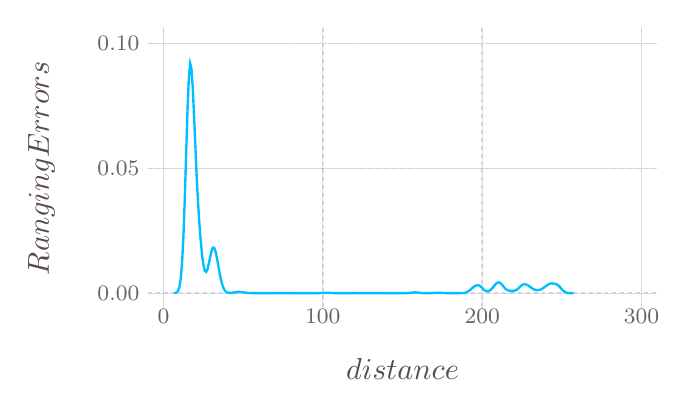
\begin{tikzpicture}[x=1mm,y=-1mm]
\definecolor{mycolor000000}{rgb}{0,0,0}
\definecolor{mycolorD0D0E0}{rgb}{0.82,0.82,0.88}
\definecolor{mycolor564A55}{rgb}{0.34,0.29,0.33}
\definecolor{mycolor6C606B}{rgb}{0.42,0.38,0.42}
\definecolor{mycolor00BFFF}{rgb}{0,0.75,1}
\definecolor{mycolor000000}{rgb}{0,0,0}
\begin{scope}
\begin{scope}
\draw (52.65,48.39) node [text=mycolor564A55,draw=mycolor000000,draw opacity=0,rotate around={-0: (0,1.81)},inner sep=0.0]{\fontsize{3.88mm}{4.66mm}\selectfont $\text{distance}$};
\end{scope}
\begin{scope}
\draw (22.31,41.72) node [text=mycolor6C606B,rotate around={-0: (30.35,1.34)},inner sep=0.0]{\fontsize{2.82mm}{3.39mm}\selectfont $\text{0}$};
\draw (42.54,41.72) node [text=mycolor6C606B,rotate around={-0: (10.12,1.34)},inner sep=0.0]{\fontsize{2.82mm}{3.39mm}\selectfont $\text{100}$};
\draw (62.77,41.72) node [text=mycolor6C606B,rotate around={-0: (-10.12,1.34)},inner sep=0.0]{\fontsize{2.82mm}{3.39mm}\selectfont $\text{200}$};
\draw (83,41.72) node [text=mycolor6C606B,rotate around={-0: (-30.35,1.34)},inner sep=0.0]{\fontsize{2.82mm}{3.39mm}\selectfont $\text{300}$};
\end{scope}
\begin{scope}
\clip  (20.31,5) -- (85,5) -- (85,40.72) -- (20.31,40.72);
\begin{scope}
\clip  (20.31,5) -- (85,5) -- (85,40.72) -- (20.31,40.72);
\path [fill=mycolor000000,fill opacity=0,draw=mycolor000000,draw opacity=0] (20.31,5) rectangle +(64.69,35.72);
\end{scope}
\begin{scope}
[dash pattern=on 0.5mm off 0.5mm,line width=0.2mm]
\path [fill=mycolor000000,draw=mycolorD0D0E0]  (20.31,38.72) -- (85,38.72);
\path [fill=mycolor000000,draw=mycolorD0D0E0]  (20.31,22.86) -- (85,22.86);
\path [fill=mycolor000000,draw=mycolorD0D0E0]  (20.31,7) -- (85,7);
\end{scope}
\begin{scope}
[dash pattern=on 0.5mm off 0.5mm,line width=0.2mm]
\path [fill=mycolor000000,draw=mycolorD0D0E0]  (22.31,5) -- (22.31,40.72);
\path [fill=mycolor000000,draw=mycolorD0D0E0]  (42.54,5) -- (42.54,40.72);
\path [fill=mycolor000000,draw=mycolorD0D0E0]  (62.77,5) -- (62.77,40.72);
\path [fill=mycolor000000,draw=mycolorD0D0E0]  (83,5) -- (83,40.72);
\end{scope}
\begin{scope}
\begin{scope}
[line width=0.3mm]
\path [fill=mycolor000000,fill opacity=0,draw=mycolor00BFFF]  (23.65,38.71) -- (23.82,38.69) -- (23.99,38.61) -- (24.16,38.41) -- (24.33,37.9) -- (24.5,36.79) -- (24.67,34.7) -- (24.84,31.29) -- (25.01,26.53) -- (25.18,20.92) -- (25.35,15.46) -- (25.52,11.38) -- (25.69,9.58) -- (25.86,10.26) -- (26.03,12.91) -- (26.2,16.63) -- (26.37,20.58) -- (26.53,24.24) -- (26.7,27.39) -- (26.87,30.04) -- (27.04,32.22) -- (27.21,33.94) -- (27.38,35.17) -- (27.55,35.87) -- (27.72,36.02) -- (27.89,35.66) -- (28.06,34.95) -- (28.23,34.1) -- (28.4,33.35) -- (28.57,32.93) -- (28.74,32.95) -- (28.91,33.41) -- (29.08,34.2) -- (29.25,35.16) -- (29.42,36.13) -- (29.59,36.97) -- (29.76,37.63) -- (29.93,38.1) -- (30.1,38.39) -- (30.27,38.56) -- (30.44,38.64) -- (30.61,38.68) -- (30.78,38.68) -- (30.95,38.67) -- (31.11,38.65) -- (31.28,38.62) -- (31.45,38.59) -- (31.62,38.56) -- (31.79,38.55) -- (31.96,38.55) -- (32.13,38.57) -- (32.3,38.59) -- (32.47,38.61) -- (32.64,38.64) -- (32.81,38.66) -- (32.98,38.68) -- (33.15,38.7) -- (33.32,38.7) -- (33.49,38.71) -- (33.66,38.71) -- (33.83,38.71) -- (34,38.71) -- (34.17,38.71) -- (34.34,38.71) -- (34.51,38.71) -- (34.68,38.71) -- (34.85,38.71) -- (35.02,38.71) -- (35.19,38.71) -- (35.36,38.71) -- (35.53,38.71) -- (35.69,38.71) -- (35.86,38.71) -- (36.03,38.71) -- (36.2,38.72) -- (36.37,38.72) -- (36.54,38.72) -- (36.71,38.72) -- (36.88,38.72) -- (37.05,38.72) -- (37.22,38.72) -- (37.39,38.72) -- (37.56,38.72) -- (37.73,38.72) -- (37.9,38.72) -- (38.07,38.72) -- (38.24,38.72) -- (38.41,38.72) -- (38.58,38.72) -- (38.75,38.72) -- (38.92,38.72) -- (39.09,38.72) -- (39.26,38.71) -- (39.43,38.71) -- (39.6,38.71) -- (39.77,38.71) -- (39.94,38.71) -- (40.11,38.71) -- (40.27,38.71) -- (40.44,38.71) -- (40.61,38.71) -- (40.78,38.71) -- (40.95,38.71) -- (41.12,38.71) -- (41.29,38.71) -- (41.46,38.71) -- (41.63,38.71) -- (41.8,38.71) -- (41.97,38.71) -- (42.14,38.7) -- (42.31,38.69) -- (42.48,38.68) -- (42.65,38.67) -- (42.82,38.67) -- (42.99,38.66) -- (43.16,38.67) -- (43.33,38.68) -- (43.5,38.69) -- (43.67,38.7) -- (43.84,38.71) -- (44.01,38.71) -- (44.18,38.71) -- (44.35,38.71) -- (44.52,38.71) -- (44.69,38.71) -- (44.85,38.71) -- (45.02,38.71) -- (45.19,38.71) -- (45.36,38.71) -- (45.53,38.71) -- (45.7,38.71) -- (45.87,38.71) -- (46.04,38.71) -- (46.21,38.71) -- (46.38,38.71) -- (46.55,38.71) -- (46.72,38.72) -- (46.89,38.72) -- (47.06,38.72) -- (47.23,38.72) -- (47.4,38.72) -- (47.57,38.72) -- (47.74,38.72) -- (47.91,38.72) -- (48.08,38.72) -- (48.25,38.72) -- (48.42,38.72) -- (48.59,38.72) -- (48.76,38.72) -- (48.93,38.72) -- (49.1,38.72) -- (49.27,38.72) -- (49.43,38.72) -- (49.6,38.72) -- (49.77,38.72) -- (49.94,38.72) -- (50.11,38.72) -- (50.28,38.72) -- (50.45,38.72) -- (50.62,38.71) -- (50.79,38.71) -- (50.96,38.71) -- (51.13,38.71) -- (51.3,38.71) -- (51.47,38.71) -- (51.64,38.71) -- (51.81,38.71) -- (51.98,38.71) -- (52.15,38.71) -- (52.32,38.71) -- (52.49,38.71) -- (52.66,38.71) -- (52.83,38.71) -- (53,38.71) -- (53.17,38.71) -- (53.34,38.7) -- (53.51,38.69) -- (53.68,38.67) -- (53.85,38.65) -- (54.01,38.63) -- (54.18,38.62) -- (54.35,38.62) -- (54.52,38.63) -- (54.69,38.65) -- (54.86,38.67) -- (55.03,38.69) -- (55.2,38.7) -- (55.37,38.71) -- (55.54,38.71) -- (55.71,38.71) -- (55.88,38.71) -- (56.05,38.71) -- (56.22,38.71) -- (56.39,38.7) -- (56.56,38.69) -- (56.73,38.68) -- (56.9,38.67) -- (57.07,38.66) -- (57.24,38.67) -- (57.41,38.67) -- (57.58,38.68) -- (57.75,38.69) -- (57.92,38.7) -- (58.09,38.71) -- (58.26,38.71) -- (58.43,38.71) -- (58.59,38.71) -- (58.76,38.71) -- (58.93,38.71) -- (59.1,38.71) -- (59.27,38.71) -- (59.44,38.71) -- (59.61,38.71) -- (59.78,38.71) -- (59.95,38.71) -- (60.12,38.71) -- (60.29,38.7) -- (60.46,38.69) -- (60.63,38.65) -- (60.8,38.6) -- (60.97,38.51) -- (61.14,38.39) -- (61.31,38.25) -- (61.48,38.1) -- (61.65,37.95) -- (61.82,37.83) -- (61.99,37.74) -- (62.16,37.7) -- (62.33,37.72) -- (62.5,37.81) -- (62.67,37.96) -- (62.84,38.13) -- (63.01,38.29) -- (63.17,38.41) -- (63.34,38.48) -- (63.51,38.48) -- (63.68,38.42) -- (63.85,38.3) -- (64.02,38.13) -- (64.19,37.92) -- (64.36,37.71) -- (64.53,37.52) -- (64.7,37.39) -- (64.87,37.35) -- (65.04,37.4) -- (65.21,37.55) -- (65.38,37.75) -- (65.55,37.97) -- (65.72,38.16) -- (65.89,38.29) -- (66.06,38.37) -- (66.23,38.4) -- (66.4,38.42) -- (66.57,38.43) -- (66.74,38.43) -- (66.91,38.4) -- (67.08,38.32) -- (67.25,38.21) -- (67.42,38.06) -- (67.59,37.89) -- (67.76,37.74) -- (67.92,37.64) -- (68.09,37.58) -- (68.26,37.59) -- (68.43,37.65) -- (68.6,37.74) -- (68.77,37.86) -- (68.94,37.98) -- (69.11,38.1) -- (69.28,38.2) -- (69.45,38.27) -- (69.62,38.32) -- (69.79,38.34) -- (69.96,38.32) -- (70.13,38.28) -- (70.3,38.21) -- (70.47,38.11) -- (70.64,37.99) -- (70.81,37.86) -- (70.98,37.73) -- (71.15,37.62) -- (71.32,37.53) -- (71.49,37.49) -- (71.66,37.48) -- (71.83,37.5) -- (72,37.52) -- (72.17,37.57) -- (72.34,37.66) -- (72.5,37.8) -- (72.67,37.97) -- (72.84,38.17) -- (73.01,38.35) -- (73.18,38.5) -- (73.35,38.6) -- (73.52,38.66) -- (73.69,38.69) -- (73.86,38.71) -- (74.03,38.71) -- (74.2,38.71) -- (74.37,38.71);
\end{scope}
\end{scope}
\end{scope}
\begin{scope}
\draw (19.3,38.72) node [text=mycolor6C606B,rotate around={-0: (-2.85,-15.86)},left,inner sep=0.0]{\fontsize{2.82mm}{3.39mm}\selectfont $\text{0.00}$};
\draw (19.3,22.86) node [text=mycolor6C606B,rotate around={-0: (-2.85,-0)},left,inner sep=0.0]{\fontsize{2.82mm}{3.39mm}\selectfont $\text{0.05}$};
\draw (19.3,7) node [text=mycolor6C606B,rotate around={-0: (-2.85,15.86)},left,inner sep=0.0]{\fontsize{2.82mm}{3.39mm}\selectfont $\text{0.10}$};
\end{scope}
\begin{scope}
\draw (8.81,20.86) node [text=mycolor564A55,draw=mycolor000000,draw opacity=0,rotate around={90: (0,2)},inner sep=0.0]{\fontsize{3.88mm}{4.66mm}\selectfont $\text{Ranging Errors}$};
\end{scope}
\end{scope}
\end{tikzpicture}

	\caption[ Missing Values vs. Real Distance ]{ Missing Values vs. Distance (cm).}
	\label{missingdistance}
\end{figure}

However, the ranging algorithm itself can provide range measurements with a DQF value of zero.
This means the measured range value should not be used.

These errors are very rare as long as only small amounts of RF interference are present.
In the nightshift-dataset less than \SI{5}{\percent} of the values where rejected because the measured value was impossibly high($> 5m$) or the DQF value was zero.

In \autoref{missingdistance} it can be seen that those errors mostly happen when the two nodes are very close to each other.
As the quadcopters cause a lot of turbulence a much bigger safety margin will be needed to avoid collisions.
Hence the distance where most measurements fail will be uncommon in real life application.


\section{Ranging Accuracy}

The most important question for the FINken project is: \enquote{Can the ranging values be used by the FINken robots?}.
To answer this question some understanding of the magnitude and distribution of the ranging error is needed.

Finding out how accurate the range values actually are proves rather difficult, as there are lots of interdependend variables that influence ranging accuracy.

Noticable disruptive effects are:
\begin{itemize}
	\item multipath effects
	\item supplied voltage
	\item RF-noise
	\item	antenna characteristics
	\item chosen frequency
\end{itemize}

To get meaningful and reproducable measurement results these effects need to be minimised or be constant over the course of the measurements.
The same antennas where used throughout all measurements and the frequency range was selected prior to the measurements used in this evaluation.

\subsection{Frequency Selection}
\label{freqencyselection}
\todo{move to implementation?}
The frequencies used by the ranging can be chosen by the user,
however frequency selection greatly influences the quality of the measurements.
This is especially true, as normal \SI{2.4}{\giga\hertz} wifi and serveral other technologies are using the same frequencies as the ranging modules the selection of a well working one is crucial to ranging performance.
In \autoref{spectrum2437} there is an analysis on the frequency utilization on wifi channel 6.
A download was started and then ended which is noticable in the waterfall plot.

Comparing the utilisation on this channel with the frequency range shown in \autoref{spectrum2483} which is right next to the first frequency used by the ranging modules several aspects can be noticed.
The noise in the frequency range for ranging is much lower then on frequencies with used for wifi—about \SI{15}{dB} in average and \SI{20}{dB} in peak.
You can also see the peak generated by the ranging modules.
The line at the center frequency \SI{2.4831}{\giga\hertz} is an artifact created by the SDR that was used, but the line at \SI{2.483}{\giga\hertz} is created by the ranging modules (which is exactly why the center frequency was chosen right next to the actual frequency).

Because of the lower utilisation of those frequencies a range of \SI{2.480}{\giga\hertz} to \SI{2.500}{\giga\hertz} has been chosen.
All the frequencies in this range look quite similar to the sample taken at \autoref{spectrum2483}.
This values have to be taken with a grain of salt.
It is really hard to reproduce what kind of RF-noise interfering with the nodes is currently generated in the swarmlab.

There are other factors impacting measurement quality that cannot be quantified easily.
At least the performance of the antennas at different frequencies cannot be directly measured in our lab.
The number of available channels in the frequency range and channel spacing are other variables that might influence ranging quality\footnote{The sourcecode and algorithms used by the modules is closed source, so we are not able to infere the effect of channel spacing and number of channels from that.}. 

In the end this means finding the right parameters for ranging frequency settings is a really hard problem, especially because measuring the ranging error for many frequencies takes a lot of labtime.
It is not viable to measure all available combinations for those parameters.


\begin{figure}[H]
	\centering
\includegraphics[width=0.9\textwidth]{figures/ch6.png}
\label{spectrum2437}
\caption{RF-Spectrum on \SI{2.437}{\giga\hertz}}
\end{figure}

\begin{figure}[H]
	\centering
\includegraphics[width=0.9\textwidth]{figures/ranging_0.png}
\label{spectrum2483}
\caption{RF-Spectrum on \SI{2.483}{\giga\hertz}}
\end{figure}


Even with the selected frequencies the measurement is only really working when the lab is empty, as basically every person in the faculty uses devices that use the \SI{2.4}{GHz} frequency range.
To create a useful evaluation all the following measurements have been made with an empty lab.
Therefore, the measurements were made at night.
However, this problem must be addressed before the sensors can be used in a real world application.
This is especially true, as the remote control is causing the worst interference with the ranging nodes observed so far and the quadcopters will not work without the remote control.

There are two possible solutions to the general problem: Either the noise in the environment needs to be reduced or the ranging nodes need to use different frequencies.


\subsection{Measurement Setup}

All the following evaluation is done by analysing the data gathered by the ranging nodes.
However, the measurements are done in a very specific manner to improve the quality of the measured data.
\begin{itemize}
	\item the nodes are lifted from the table to minimise multipath effects
	\item a stable 3.3V input voltage is provided by different voltage regulators, the battery slots are not used
	\item antennas are always used in the same orientation
	\item measurements are not taken in the working hours of the faculty (mostly deep at night) when the least ammount of RF interference by \SI{2.4}{GHz} devices can be expected
\end{itemize}

\begin{figure}[H]
	\centering
	\includegraphics[width=0.9\textwidth]{figures/messaufbau.png}
	\caption[ Measurement Setup ]{ Measurement Setup. RaspberryPi microcomputer is connected to the ranging node via I2C. }
	\label{aufbau}
\end{figure}

\subsection{Data Sets}

The evaluation of the ranging nodes relies on three datasets that have been recorded.
Before those datasets were recorded many other measurements where made.
These measurements are not directly used in the evaluation, but for finding disrupting influences that would compromise the evaluation data.

To avoid confusion the measured range in the dataset is called \enquote{range} and the reference measurement for the distance is called \enquote{distance}.
The same nomenclature can be found in this thesis.
All the distance and range values used in the datasets are in \emph{cm}.

\subsubsection*{\enquote{Nightshift}}
RF-noise greatly influences the ranging measurements and almost everyone in the faculty uses \SI{2.4}{GHz} devices.
As a consequence, data recorded at night is less noisy than data recorded during daytime.
Because of this fact all the data was recorded at nighttime.

The \enquote{Nightshift}-dataset consists of range values measured for distances between \SI{16}{cm} and \SI{250}{cm} in \SI{2}{cm} intervals.
For each of the distances 200 range values have been measured.

\subsubsection*{Angle Dataset}
To determine the influence of rotation another dataset has been recorded at \SI{50}{cm}, \SI{100}{cm} and \SI{150}{cm}.
At each distance one of the sensors was rotated in \SI{30}{\degree}-steps.

\subsubsection*{Symmetry}
To check if the range measurements are symmetrical the remote measurement capabilities of the ranging nodes where utilized.
Three nodes where used to generate more data, while still beeing able to automatically measure at nighttime.
It was intended to also evaluate the triangle equation with this data, however this has proven to be impractical.

\begin{table}[h]
	\centering	
	\begin{tabular}{l | r | r}
	           & RMSE (cm) & Samples \\ \hline
	Nightshift & 23.75     & 23600   \\ 
	Angle      & 42.74     & 9597    \\
	Symmetry   & 32.58     & 17999   \\
	
	\end{tabular}

	\caption{Dataset comparison}
	\label{datasets}
	
\end{table}

\subsection{Relationship between Distance and Measured Range}

It is important to know how the ranging nodes behave at different distances.
For this analysis the \enquote{nightshift}-dataset is used.

In \autoref{corridor} for each possible range value an interval is showed in which the real distance is located with a confidence of \SI{90}{\percent}.
The average size of this interval is \SI{50}{cm} for all range values smaller than \SI{2}{m}.
It is also notable that the intervals get bigger for greater distances, which may not be suprising.
For ranges below \SI{1}{m} the interval is only \SI{38}{cm} big, for ranges between \SI{1}{m} and \SI{2}{m} the average interval-size is \SI{60}{cm}.

Another notable fact is that the ideal value (showed as blue line) is always within the intervals.

\begin{figure}[h]
	\centering
	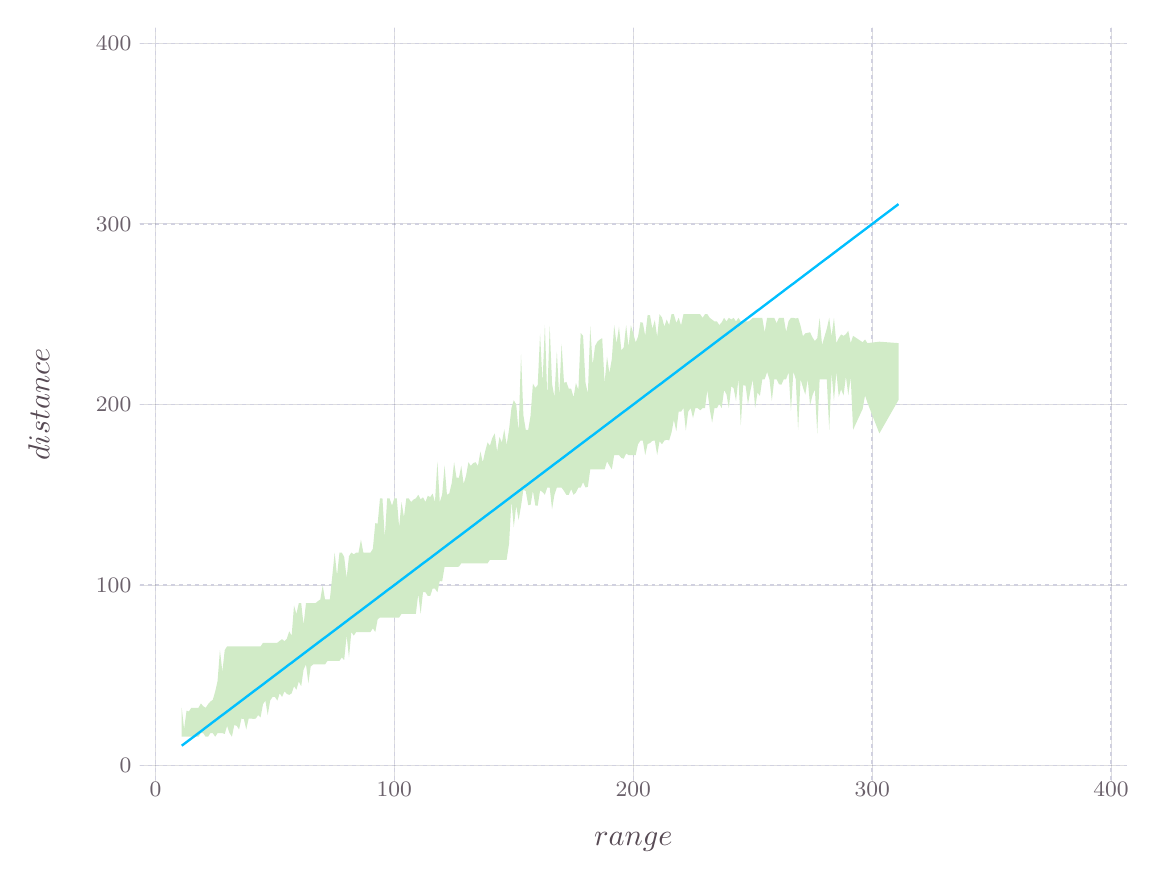
\begin{tikzpicture}[x=1mm,y=-1mm]
\definecolor{mycolor00BFFF}{rgb}{0,0.75,1}
\definecolor{mycolor000000}{rgb}{0,0,0}
\definecolor{mycolorD0D0E0}{rgb}{0.82,0.82,0.88}
\definecolor{mycolor564A55}{rgb}{0.34,0.29,0.33}
\definecolor{mycolorD1EAC7}{rgb}{0.82,0.92,0.78}
\definecolor{mycolor6C606B}{rgb}{0.42,0.38,0.42}
\definecolor{mycolor000000}{rgb}{0,0,0}
\begin{scope}
\begin{scope}
\draw (82.32,108.39) node [text=mycolor564A55,draw=mycolor000000,draw opacity=0,rotate around={-0: (0,1.81)},inner sep=0.0]{\fontsize{3.88mm}{4.66mm}\selectfont $\text{range}$};
\end{scope}
\begin{scope}
\draw (21.63,101.72) node [text=mycolor6C606B,rotate around={-0: (60.68,1.34)},inner sep=0.0]{\fontsize{2.82mm}{3.39mm}\selectfont $\text{0}$};
\draw (51.97,101.72) node [text=mycolor6C606B,rotate around={-0: (30.34,1.34)},inner sep=0.0]{\fontsize{2.82mm}{3.39mm}\selectfont $\text{100}$};
\draw (82.32,101.72) node [text=mycolor6C606B,rotate around={-0: (0,1.34)},inner sep=0.0]{\fontsize{2.82mm}{3.39mm}\selectfont $\text{200}$};
\draw (112.66,101.72) node [text=mycolor6C606B,rotate around={-0: (-30.34,1.34)},inner sep=0.0]{\fontsize{2.82mm}{3.39mm}\selectfont $\text{300}$};
\draw (143,101.72) node [text=mycolor6C606B,rotate around={-0: (-60.68,1.34)},inner sep=0.0]{\fontsize{2.82mm}{3.39mm}\selectfont $\text{400}$};
\end{scope}
\begin{scope}
\clip  (19.63,5) -- (145,5) -- (145,100.72) -- (19.63,100.72);
\begin{scope}
\clip  (19.63,5) -- (145,5) -- (145,100.72) -- (19.63,100.72);
\path [fill=mycolor000000,fill opacity=0,draw=mycolor000000,draw opacity=0] (19.63,5) rectangle +(125.37,95.72);
\end{scope}
\begin{scope}
[dash pattern=on 0.5mm off 0.5mm,line width=0.2mm]
\path [fill=mycolor000000,draw=mycolorD0D0E0]  (19.63,98.71) -- (145,98.71);
\path [fill=mycolor000000,draw=mycolorD0D0E0]  (19.63,75.79) -- (145,75.79);
\path [fill=mycolor000000,draw=mycolorD0D0E0]  (19.63,52.86) -- (145,52.86);
\path [fill=mycolor000000,draw=mycolorD0D0E0]  (19.63,29.93) -- (145,29.93);
\path [fill=mycolor000000,draw=mycolorD0D0E0]  (19.63,7) -- (145,7);
\end{scope}
\begin{scope}
[dash pattern=on 0.5mm off 0.5mm,line width=0.2mm]
\path [fill=mycolor000000,draw=mycolorD0D0E0]  (21.63,5) -- (21.63,100.72);
\path [fill=mycolor000000,draw=mycolorD0D0E0]  (51.97,5) -- (51.97,100.72);
\path [fill=mycolor000000,draw=mycolorD0D0E0]  (82.32,5) -- (82.32,100.72);
\path [fill=mycolor000000,draw=mycolorD0D0E0]  (112.66,5) -- (112.66,100.72);
\path [fill=mycolor000000,draw=mycolorD0D0E0]  (143,5) -- (143,100.72);
\end{scope}
\begin{scope}
\begin{scope}
[line width=0.3mm]
\path [fill=mycolorD1EAC7,draw=mycolor000000,draw opacity=0]  (116,52.28) -- (113.57,56.53) -- (112.05,52.63) -- (111.75,51.71) -- (111.44,53.43) -- (110.23,56.07) -- (109.93,49.4) -- (109.62,51.67) -- (109.32,49.3) -- (109.02,51.71) -- (108.71,50.93) -- (108.41,51.85) -- (108.11,48.73) -- (107.8,52.4) -- (107.5,48.87) -- (107.2,56.09) -- (106.89,49.65) -- (106.29,49.65) -- (105.98,49.65) -- (105.68,56.53) -- (105.38,50.93) -- (105.07,51.71) -- (104.77,52.97) -- (104.47,49.65) -- (104.16,51.6) -- (103.86,50.68) -- (103.56,49.65) -- (103.25,56.07) -- (102.95,49.65) -- (102.65,48.66) -- (102.34,53.66) -- (102.04,48.73) -- (101.73,49.65) -- (101.43,49.65) -- (101.13,50.34) -- (100.82,50.29) -- (100.52,49.65) -- (100.22,49.65) -- (99.91,52.4) -- (99.61,49.65) -- (99.31,48.73) -- (99,49.65) -- (98.7,49.65) -- (98.4,51.76) -- (98.09,51.34) -- (97.79,53.32) -- (97.49,49.65) -- (97.18,51.18) -- (96.88,52.81) -- (96.58,50.47) -- (96.27,50.4) -- (95.97,55.52) -- (95.67,49.65) -- (95.36,52.4) -- (95.06,50.79) -- (94.76,50.56) -- (94.45,53.32) -- (94.15,51.57) -- (93.85,51.02) -- (93.54,53.32) -- (93.24,52.72) -- (92.94,53.32) -- (92.63,53.32) -- (92.33,55.15) -- (92.03,53.48) -- (91.72,51.02) -- (91.42,53.32) -- (91.12,53.32) -- (90.81,53.59) -- (90.51,53.32) -- (90.2,53.32) -- (89.9,54.58) -- (89.6,53.32) -- (89.29,53.77) -- (88.99,56.18) -- (88.69,53.32) -- (88.38,53.77) -- (88.08,53.77) -- (87.78,56.25) -- (87.47,54.81) -- (87.17,56.43) -- (86.87,57.42) -- (86.56,57.33) -- (86.26,57.44) -- (85.96,57.9) -- (85.65,57.53) -- (85.35,59.28) -- (85.05,57.44) -- (84.74,57.47) -- (84.44,57.76) -- (84.14,57.86) -- (83.83,59.28) -- (83.53,57.44) -- (83.23,57.44) -- (82.92,57.9) -- (82.62,59.28) -- (82.32,59.28) -- (82.01,59.28) -- (81.71,59.28) -- (81.41,59.07) -- (81.1,59.74) -- (80.8,59.64) -- (80.5,59.28) -- (80.19,59.28) -- (79.89,59.28) -- (79.59,61.11) -- (79.28,60.61) -- (78.98,60.08) -- (78.67,61.11) -- (78.37,61.11) -- (78.07,61.11) -- (77.76,61.11) -- (77.46,61.11) -- (77.16,61.11) -- (76.85,61.11) -- (76.55,63.31) -- (76.25,63.4) -- (75.94,62.72) -- (75.64,63.4) -- (75.34,63.4) -- (75.03,64.05) -- (74.73,64.32) -- (74.43,63.61) -- (74.12,64.32) -- (73.82,64.32) -- (73.52,63.86) -- (73.21,63.4) -- (72.91,63.4) -- (72.61,63.4) -- (72.3,64.32) -- (72,66.16) -- (71.7,63.4) -- (71.39,63.4) -- (71.09,64.32) -- (70.79,63.98) -- (70.48,63.77) -- (70.18,65.7) -- (69.88,65.7) -- (69.57,63.82) -- (69.27,65.61) -- (68.97,65.63) -- (68.66,63.86) -- (68.36,63.68) -- (68.06,65.74) -- (67.75,67.53) -- (67.45,65.7) -- (67.14,68.45) -- (66.84,65.12) -- (66.54,70.51) -- (66.23,72.58) -- (65.93,72.58) -- (65.63,72.58) -- (65.32,72.58) -- (65.02,72.58) -- (64.72,72.58) -- (64.41,72.58) -- (64.11,72.58) -- (63.81,73.03) -- (63.5,73.03) -- (63.2,73.03) -- (62.9,73.03) -- (62.59,73.03) -- (62.29,73.03) -- (61.99,73.03) -- (61.68,73.03) -- (61.38,73.03) -- (61.08,73.03) -- (60.77,73.03) -- (60.47,73.03) -- (60.17,73.45) -- (59.86,73.49) -- (59.56,73.49) -- (59.26,73.49) -- (58.95,73.49) -- (58.65,73.49) -- (58.35,73.49) -- (58.04,75.33) -- (57.74,75.26) -- (57.44,76.7) -- (57.13,76.24) -- (56.83,76.24) -- (56.53,77.16) -- (56.22,77.16) -- (55.92,76.7) -- (55.61,76.7) -- (55.31,79.45) -- (55.01,76.93) -- (54.7,79.45) -- (54.4,79.45) -- (54.1,79.45) -- (53.79,79.45) -- (53.49,79.45) -- (53.19,79.45) -- (52.88,79.45) -- (52.58,79.91) -- (52.28,79.91) -- (51.97,79.91) -- (51.67,79.91) -- (51.37,79.91) -- (51.06,79.91) -- (50.76,79.91) -- (50.46,79.91) -- (50.15,79.91) -- (49.85,80.14) -- (49.55,81.75) -- (49.24,81.29) -- (48.94,81.75) -- (48.64,81.75) -- (48.33,81.75) -- (48.03,81.75) -- (47.73,81.75) -- (47.42,81.75) -- (47.12,81.75) -- (46.82,82.21) -- (46.51,81.75) -- (46.21,84.96) -- (45.91,82.21) -- (45.6,85.32) -- (45.3,84.98) -- (45,85.42) -- (44.69,85.42) -- (44.39,85.42) -- (44.08,85.42) -- (43.78,85.42) -- (43.48,85.42) -- (43.17,85.87) -- (42.87,85.87) -- (42.57,85.87) -- (42.26,85.87) -- (41.96,85.87) -- (41.66,85.87) -- (41.35,86.13) -- (41.05,88.26) -- (40.75,85.87) -- (40.44,86.54) -- (40.14,88.63) -- (39.84,88.03) -- (39.53,89.08) -- (39.23,88.63) -- (38.93,89.54) -- (38.62,89.73) -- (38.32,89.61) -- (38.02,89.29) -- (37.71,90) -- (37.41,89.54) -- (37.11,90.46) -- (36.8,90) -- (36.5,90) -- (36.2,90.46) -- (35.89,92.29) -- (35.59,90.46) -- (35.29,90.92) -- (34.98,92.59) -- (34.68,92.29) -- (34.38,92.75) -- (34.07,92.78) -- (33.77,92.75) -- (33.47,92.75) -- (33.16,94.13) -- (32.86,92.8) -- (32.55,92.75) -- (32.25,94.13) -- (31.95,93.67) -- (31.64,93.56) -- (31.34,95.05) -- (31.04,94.59) -- (30.73,93.67) -- (30.43,94.7) -- (30.13,94.59) -- (29.82,94.59) -- (29.52,94.59) -- (29.22,95.05) -- (28.91,94.59) -- (28.61,94.59) -- (28.31,95.05) -- (28,95.05) -- (27.7,94.59) -- (27.4,94.59) -- (27.09,95.05) -- (26.79,95.05) -- (26.49,95.05) -- (26.18,95.05) -- (25.88,95.05) -- (25.58,95.05) -- (25.27,95.05) -- (24.97,95.05) -- (24.97,91.38) -- (25.27,94.06) -- (25.58,91.74) -- (25.88,91.84) -- (26.18,91.38) -- (26.49,91.38) -- (26.79,91.38) -- (27.09,91.38) -- (27.4,90.83) -- (27.7,91.17) -- (28,91.38) -- (28.31,90.92) -- (28.61,90.58) -- (28.91,90.37) -- (29.22,89.31) -- (29.52,87.98) -- (29.82,84.04) -- (30.13,86.79) -- (30.43,84.04) -- (30.73,83.58) -- (31.04,83.58) -- (31.34,83.58) -- (31.64,83.58) -- (31.95,83.58) -- (32.25,83.58) -- (32.55,83.58) -- (32.86,83.58) -- (33.16,83.58) -- (33.47,83.58) -- (33.77,83.58) -- (34.07,83.58) -- (34.38,83.58) -- (34.68,83.58) -- (34.98,83.58) -- (35.29,83.12) -- (35.59,83.12) -- (35.89,83.12) -- (36.2,83.12) -- (36.5,83.12) -- (36.8,83.12) -- (37.11,83.12) -- (37.41,82.87) -- (37.71,82.66) -- (38.02,82.92) -- (38.32,82.6) -- (38.62,81.66) -- (38.93,82.21) -- (39.23,78.38) -- (39.53,79.45) -- (39.84,78.08) -- (40.14,78.08) -- (40.44,80.83) -- (40.75,78.08) -- (41.05,78.08) -- (41.35,78.08) -- (41.66,78.08) -- (41.96,78.08) -- (42.26,77.83) -- (42.57,77.62) -- (42.87,75.83) -- (43.17,77.62) -- (43.48,77.62) -- (43.78,77.62) -- (44.08,74.73) -- (44.39,71.66) -- (44.69,74.55) -- (45,71.66) -- (45.3,71.66) -- (45.6,72.21) -- (45.91,74.87) -- (46.21,72.12) -- (46.51,71.66) -- (46.82,71.89) -- (47.12,71.66) -- (47.42,71.66) -- (47.73,70.01) -- (48.03,71.66) -- (48.33,71.66) -- (48.64,71.66) -- (48.94,71.66) -- (49.24,71.2) -- (49.55,67.92) -- (49.85,67.99) -- (50.15,64.78) -- (50.46,64.78) -- (50.76,69.73) -- (51.06,64.78) -- (51.37,64.78) -- (51.67,65.7) -- (51.97,64.78) -- (52.28,64.78) -- (52.58,68.45) -- (52.88,65.24) -- (53.19,67.17) -- (53.49,64.78) -- (53.79,64.78) -- (54.1,65.24) -- (54.4,64.94) -- (54.7,64.78) -- (55.01,64.32) -- (55.31,64.9) -- (55.61,64.64) -- (55.92,65.24) -- (56.22,64.44) -- (56.53,64.62) -- (56.83,64.16) -- (57.13,65.24) -- (57.44,60.1) -- (57.74,65.24) -- (58.04,64.32) -- (58.35,60.58) -- (58.65,64.32) -- (58.95,64.14) -- (59.26,62.83) -- (59.56,60.19) -- (59.86,62.14) -- (60.17,62.17) -- (60.47,60.65) -- (60.77,62.95) -- (61.08,61.89) -- (61.38,60.19) -- (61.68,60.65) -- (61.99,60.29) -- (62.29,60.19) -- (62.59,60.65) -- (62.9,58.82) -- (63.2,60.19) -- (63.5,58.82) -- (63.81,57.67) -- (64.11,58.09) -- (64.41,57.1) -- (64.72,56.53) -- (65.02,58.82) -- (65.32,56.98) -- (65.63,57.67) -- (65.93,56.02) -- (66.23,57.99) -- (66.54,56.02) -- (66.84,53.32) -- (67.14,52.31) -- (67.45,52.86) -- (67.75,56.3) -- (68.06,46.48) -- (68.36,54.23) -- (68.66,56.07) -- (68.97,56.07) -- (69.27,54.28) -- (69.57,50.2) -- (69.88,50.75) -- (70.18,50.38) -- (70.48,43.87) -- (70.79,50.11) -- (71.09,42.75) -- (71.39,51.94) -- (71.7,42.86) -- (72,50.24) -- (72.3,51.89) -- (72.61,46.14) -- (72.91,51.78) -- (73.21,45.15) -- (73.52,50.11) -- (73.82,49.99) -- (74.12,50.84) -- (74.43,50.86) -- (74.73,51.94) -- (75.03,50.11) -- (75.34,51.02) -- (75.64,43.78) -- (75.94,44.14) -- (76.25,50.11) -- (76.55,51.48) -- (76.85,42.98) -- (77.16,47.81) -- (77.46,45.43) -- (77.76,44.88) -- (78.07,44.6) -- (78.37,44.44) -- (78.67,50.11) -- (78.98,46.78) -- (79.28,48.87) -- (79.59,47.08) -- (79.89,42.77) -- (80.19,45.11) -- (80.5,42.98) -- (80.8,45.98) -- (81.1,45.61) -- (81.41,42.77) -- (81.71,45.52) -- (82.01,42.77) -- (82.32,43.87) -- (82.62,44.97) -- (82.92,44.24) -- (83.23,42.4) -- (83.53,42.47) -- (83.83,44.14) -- (84.14,41.48) -- (84.44,41.53) -- (84.74,43.23) -- (85.05,42.15) -- (85.35,44.26) -- (85.65,41.39) -- (85.96,41.81) -- (86.26,42.95) -- (86.56,42.08) -- (86.87,42.77) -- (87.17,41.39) -- (87.47,41.39) -- (87.78,42.49) -- (88.08,41.85) -- (88.38,42.81) -- (88.69,41.39) -- (88.99,41.39) -- (89.29,41.39) -- (89.6,41.39) -- (89.9,41.39) -- (90.2,41.39) -- (90.51,41.39) -- (90.81,41.39) -- (91.12,41.85) -- (91.42,41.39) -- (91.72,41.39) -- (92.03,41.85) -- (92.33,42.08) -- (92.63,42.31) -- (92.94,42.31) -- (93.24,42.77) -- (93.54,42.42) -- (93.85,41.85) -- (94.15,42.31) -- (94.45,41.85) -- (94.76,42.06) -- (95.06,41.85) -- (95.36,42.31) -- (95.67,41.85) -- (95.97,42.31) -- (96.27,42.31) -- (96.58,42.31) -- (96.88,42.31) -- (97.18,42.15) -- (97.49,41.85) -- (97.79,41.85) -- (98.09,41.85) -- (98.4,41.85) -- (98.7,41.85) -- (99,43.69) -- (99.31,41.85) -- (99.61,41.85) -- (99.91,41.85) -- (100.22,41.85) -- (100.52,42.52) -- (100.82,41.85) -- (101.13,41.85) -- (101.43,41.85) -- (101.73,43.64) -- (102.04,42.26) -- (102.34,41.85) -- (102.65,41.85) -- (102.95,41.94) -- (103.25,41.85) -- (103.56,42.86) -- (103.86,44.19) -- (104.16,43.82) -- (104.47,43.75) -- (104.77,43.69) -- (105.07,44.33) -- (105.38,44.79) -- (105.68,44.42) -- (105.98,41.85) -- (106.29,45.29) -- (106.89,43.23) -- (107.2,41.85) -- (107.5,44.19) -- (107.8,41.85) -- (108.11,45.06) -- (108.41,44.42) -- (108.71,43.96) -- (109.02,44.14) -- (109.32,43.92) -- (109.62,43.5) -- (109.93,45.06) -- (110.23,44.14) -- (111.44,44.95) -- (111.75,44.6) -- (112.05,45.06) -- (113.57,44.88) -- (116,45.06) -- cycle;
\end{scope}
\begin{scope}
[line width=0.3mm]
\path [fill=mycolor000000,fill opacity=0,draw=mycolor00BFFF]  (24.97,96.19) -- (25.27,95.96) -- (25.58,95.73) -- (25.88,95.5) -- (26.18,95.28) -- (26.49,95.05) -- (26.79,94.82) -- (27.09,94.59) -- (27.4,94.36) -- (27.7,94.13) -- (28,93.9) -- (28.31,93.67) -- (28.61,93.44) -- (28.91,93.21) -- (29.22,92.98) -- (29.52,92.75) -- (29.82,92.52) -- (30.13,92.29) -- (30.43,92.07) -- (30.73,91.84) -- (31.04,91.61) -- (31.34,91.38) -- (31.64,91.15) -- (31.95,90.92) -- (32.25,90.69) -- (32.55,90.46) -- (32.86,90.23) -- (33.16,90) -- (33.47,89.77) -- (33.77,89.54) -- (34.07,89.31) -- (34.38,89.08) -- (34.68,88.86) -- (34.98,88.63) -- (35.29,88.4) -- (35.59,88.17) -- (35.89,87.94) -- (36.2,87.71) -- (36.5,87.48) -- (36.8,87.25) -- (37.11,87.02) -- (37.41,86.79) -- (37.71,86.56) -- (38.02,86.33) -- (38.32,86.1) -- (38.62,85.87) -- (38.93,85.65) -- (39.23,85.42) -- (39.53,85.19) -- (39.84,84.96) -- (40.14,84.73) -- (40.44,84.5) -- (40.75,84.27) -- (41.05,84.04) -- (41.35,83.81) -- (41.66,83.58) -- (41.96,83.35) -- (42.26,83.12) -- (42.57,82.89) -- (42.87,82.66) -- (43.17,82.44) -- (43.48,82.21) -- (43.78,81.98) -- (44.08,81.75) -- (44.39,81.52) -- (44.69,81.29) -- (45,81.06) -- (45.3,80.83) -- (45.6,80.6) -- (45.91,80.37) -- (46.21,80.14) -- (46.51,79.91) -- (46.82,79.68) -- (47.12,79.45) -- (47.42,79.23) -- (47.73,79) -- (48.03,78.77) -- (48.33,78.54) -- (48.64,78.31) -- (48.94,78.08) -- (49.24,77.85) -- (49.55,77.62) -- (49.85,77.39) -- (50.15,77.16) -- (50.46,76.93) -- (50.76,76.7) -- (51.06,76.47) -- (51.37,76.24) -- (51.67,76.02) -- (51.97,75.79) -- (52.28,75.56) -- (52.58,75.33) -- (52.88,75.1) -- (53.19,74.87) -- (53.49,74.64) -- (53.79,74.41) -- (54.1,74.18) -- (54.4,73.95) -- (54.7,73.72) -- (55.01,73.49) -- (55.31,73.26) -- (55.61,73.03) -- (55.92,72.81) -- (56.22,72.58) -- (56.53,72.35) -- (56.83,72.12) -- (57.13,71.89) -- (57.44,71.66) -- (57.74,71.43) -- (58.04,71.2) -- (58.35,70.97) -- (58.65,70.74) -- (58.95,70.51) -- (59.26,70.28) -- (59.56,70.05) -- (59.86,69.82) -- (60.17,69.6) -- (60.47,69.37) -- (60.77,69.14) -- (61.08,68.91) -- (61.38,68.68) -- (61.68,68.45) -- (61.99,68.22) -- (62.29,67.99) -- (62.59,67.76) -- (62.9,67.53) -- (63.2,67.3) -- (63.5,67.07) -- (63.81,66.84) -- (64.11,66.61) -- (64.41,66.39) -- (64.72,66.16) -- (65.02,65.93) -- (65.32,65.7) -- (65.63,65.47) -- (65.93,65.24) -- (66.23,65.01) -- (66.54,64.78) -- (66.84,64.55) -- (67.14,64.32) -- (67.45,64.09) -- (67.75,63.86) -- (68.06,63.63) -- (68.36,63.4) -- (68.66,63.18) -- (68.97,62.95) -- (69.27,62.72) -- (69.57,62.49) -- (69.88,62.26) -- (70.18,62.03) -- (70.48,61.8) -- (70.79,61.57) -- (71.09,61.34) -- (71.39,61.11) -- (71.7,60.88) -- (72,60.65) -- (72.3,60.42) -- (72.61,60.19) -- (72.91,59.97) -- (73.21,59.74) -- (73.52,59.51) -- (73.82,59.28) -- (74.12,59.05) -- (74.43,58.82) -- (74.73,58.59) -- (75.03,58.36) -- (75.34,58.13) -- (75.64,57.9) -- (75.94,57.67) -- (76.25,57.44) -- (76.55,57.21) -- (76.85,56.98) -- (77.16,56.76) -- (77.46,56.53) -- (77.76,56.3) -- (78.07,56.07) -- (78.37,55.84) -- (78.67,55.61) -- (78.98,55.38) -- (79.28,55.15) -- (79.59,54.92) -- (79.89,54.69) -- (80.19,54.46) -- (80.5,54.23) -- (80.8,54) -- (81.1,53.77) -- (81.41,53.55) -- (81.71,53.32) -- (82.01,53.09) -- (82.32,52.86) -- (82.62,52.63) -- (82.92,52.4) -- (83.23,52.17) -- (83.53,51.94) -- (83.83,51.71) -- (84.14,51.48) -- (84.44,51.25) -- (84.74,51.02) -- (85.05,50.79) -- (85.35,50.56) -- (85.65,50.34) -- (85.96,50.11) -- (86.26,49.88) -- (86.56,49.65) -- (86.87,49.42) -- (87.17,49.19) -- (87.47,48.96) -- (87.78,48.73) -- (88.08,48.5) -- (88.38,48.27) -- (88.69,48.04) -- (88.99,47.81) -- (89.29,47.58) -- (89.6,47.35) -- (89.9,47.13) -- (90.2,46.9) -- (90.51,46.67) -- (90.81,46.44) -- (91.12,46.21) -- (91.42,45.98) -- (91.72,45.75) -- (92.03,45.52) -- (92.33,45.29) -- (92.63,45.06) -- (92.94,44.83) -- (93.24,44.6) -- (93.54,44.37) -- (93.85,44.14) -- (94.15,43.92) -- (94.45,43.69) -- (94.76,43.46) -- (95.06,43.23) -- (95.36,43) -- (95.67,42.77) -- (95.97,42.54) -- (96.27,42.31) -- (96.58,42.08) -- (96.88,41.85) -- (97.18,41.62) -- (97.49,41.39) -- (97.79,41.16) -- (98.09,40.93) -- (98.4,40.71) -- (98.7,40.48) -- (99,40.25) -- (99.31,40.02) -- (99.61,39.79) -- (99.91,39.56) -- (100.22,39.33) -- (100.52,39.1) -- (100.82,38.87) -- (101.13,38.64) -- (101.43,38.41) -- (101.73,38.18) -- (102.04,37.95) -- (102.34,37.72) -- (102.65,37.5) -- (102.95,37.27) -- (103.25,37.04) -- (103.56,36.81) -- (103.86,36.58) -- (104.16,36.35) -- (104.47,36.12) -- (104.77,35.89) -- (105.07,35.66) -- (105.38,35.43) -- (105.68,35.2) -- (105.98,34.97) -- (106.29,34.74) -- (106.89,34.29) -- (107.2,34.06) -- (107.5,33.83) -- (107.8,33.6) -- (108.11,33.37) -- (108.41,33.14) -- (108.71,32.91) -- (109.02,32.68) -- (109.32,32.45) -- (109.62,32.22) -- (109.93,31.99) -- (110.23,31.76) -- (111.44,30.85) -- (111.75,30.62) -- (112.05,30.39) -- (113.57,29.24) -- (116,27.41);
\end{scope}
\end{scope}
\end{scope}
\begin{scope}
\draw (18.63,98.71) node [text=mycolor6C606B,rotate around={-0: (-2.51,-45.86)},left,inner sep=0.0]{\fontsize{2.82mm}{3.39mm}\selectfont $\text{0}$};
\draw (18.63,75.79) node [text=mycolor6C606B,rotate around={-0: (-2.51,-22.93)},left,inner sep=0.0]{\fontsize{2.82mm}{3.39mm}\selectfont $\text{100}$};
\draw (18.63,52.86) node [text=mycolor6C606B,rotate around={-0: (-2.51,0)},left,inner sep=0.0]{\fontsize{2.82mm}{3.39mm}\selectfont $\text{200}$};
\draw (18.63,29.93) node [text=mycolor6C606B,rotate around={-0: (-2.51,22.93)},left,inner sep=0.0]{\fontsize{2.82mm}{3.39mm}\selectfont $\text{300}$};
\draw (18.63,7) node [text=mycolor6C606B,rotate around={-0: (-2.51,45.86)},left,inner sep=0.0]{\fontsize{2.82mm}{3.39mm}\selectfont $\text{400}$};
\end{scope}
\begin{scope}
\draw (8.81,50.86) node [text=mycolor564A55,draw=mycolor000000,draw opacity=0,rotate around={90: (0,2)},inner sep=0.0]{\fontsize{3.88mm}{4.66mm}\selectfont $\text{distance}$};
\end{scope}
\end{scope}
\end{tikzpicture}

	\caption[ Measured range vs. Real Distance ]{Measured range (cm) vs. Real Distance (cm). In this diagram for each possible range value the 0.9-quantile of the real distances are plottet as green area. The blue line shows the ideal value.}
	\label{corridor}
\end{figure}

\begin{figure}[h]
	\centering
	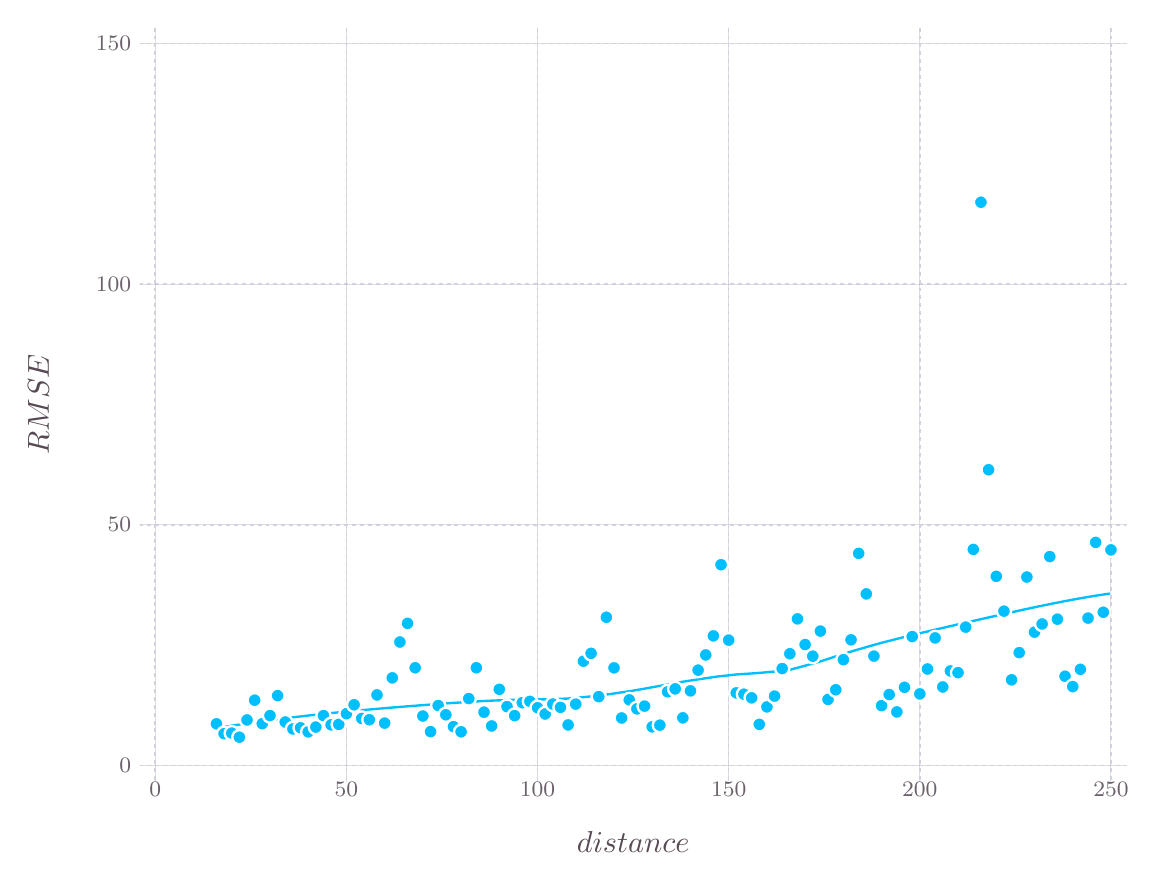
\begin{tikzpicture}[x=1mm,y=-1mm]
\definecolor{mycolor000000}{rgb}{0,0,0}
\definecolor{mycolorD0D0E0}{rgb}{0.82,0.82,0.88}
\definecolor{mycolor564A55}{rgb}{0.34,0.29,0.33}
\definecolor{mycolor6C606B}{rgb}{0.42,0.38,0.42}
\definecolor{mycolor00BFFF}{rgb}{0,0.75,1}
\definecolor{mycolor000000}{rgb}{0,0,0}
\definecolor{mycolorFFFFFF}{rgb}{1,1,1}
\begin{scope}
\begin{scope}
\draw (82.32,108.39) node [text=mycolor564A55,draw=mycolor000000,draw opacity=0,rotate around={-0: (0,1.81)},inner sep=0.0]{\fontsize{3.88mm}{4.66mm}\selectfont $\text{distance}$};
\end{scope}
\begin{scope}
\draw (21.63,101.72) node [text=mycolor6C606B,rotate around={-0: (60.68,1.34)},inner sep=0.0]{\fontsize{2.82mm}{3.39mm}\selectfont $\text{0}$};
\draw (45.91,101.72) node [text=mycolor6C606B,rotate around={-0: (36.41,1.34)},inner sep=0.0]{\fontsize{2.82mm}{3.39mm}\selectfont $\text{50}$};
\draw (70.18,101.72) node [text=mycolor6C606B,rotate around={-0: (12.14,1.34)},inner sep=0.0]{\fontsize{2.82mm}{3.39mm}\selectfont $\text{100}$};
\draw (94.45,101.72) node [text=mycolor6C606B,rotate around={-0: (-12.14,1.34)},inner sep=0.0]{\fontsize{2.82mm}{3.39mm}\selectfont $\text{150}$};
\draw (118.73,101.72) node [text=mycolor6C606B,rotate around={-0: (-36.41,1.34)},inner sep=0.0]{\fontsize{2.82mm}{3.39mm}\selectfont $\text{200}$};
\draw (143,101.72) node [text=mycolor6C606B,rotate around={-0: (-60.68,1.34)},inner sep=0.0]{\fontsize{2.82mm}{3.39mm}\selectfont $\text{250}$};
\end{scope}
\begin{scope}
\clip  (19.63,5) -- (145,5) -- (145,100.72) -- (19.63,100.72);
\begin{scope}
\clip  (19.63,5) -- (145,5) -- (145,100.72) -- (19.63,100.72);
\path [fill=mycolor000000,fill opacity=0,draw=mycolor000000,draw opacity=0] (19.63,5) rectangle +(125.37,95.72);
\end{scope}
\begin{scope}
[dash pattern=on 0.5mm off 0.5mm,line width=0.2mm]
\path [fill=mycolor000000,draw=mycolorD0D0E0]  (19.63,98.71) -- (145,98.71);
\path [fill=mycolor000000,draw=mycolorD0D0E0]  (19.63,68.14) -- (145,68.14);
\path [fill=mycolor000000,draw=mycolorD0D0E0]  (19.63,37.57) -- (145,37.57);
\path [fill=mycolor000000,draw=mycolorD0D0E0]  (19.63,7) -- (145,7);
\end{scope}
\begin{scope}
[dash pattern=on 0.5mm off 0.5mm,line width=0.2mm]
\path [fill=mycolor000000,draw=mycolorD0D0E0]  (21.63,5) -- (21.63,100.72);
\path [fill=mycolor000000,draw=mycolorD0D0E0]  (45.91,5) -- (45.91,100.72);
\path [fill=mycolor000000,draw=mycolorD0D0E0]  (70.18,5) -- (70.18,100.72);
\path [fill=mycolor000000,draw=mycolorD0D0E0]  (94.45,5) -- (94.45,100.72);
\path [fill=mycolor000000,draw=mycolorD0D0E0]  (118.73,5) -- (118.73,100.72);
\path [fill=mycolor000000,draw=mycolorD0D0E0]  (143,5) -- (143,100.72);
\end{scope}
\begin{scope}
\begin{scope}
[line width=0.3mm]
\path [fill=mycolor000000,fill opacity=0,draw=mycolor00BFFF]  (29.4,93.96) -- (29.55,93.93) -- (29.7,93.91) -- (29.85,93.88) -- (30.01,93.86) -- (30.16,93.83) -- (30.31,93.81) -- (30.46,93.78) -- (30.61,93.76) -- (30.76,93.74) -- (30.92,93.71) -- (31.07,93.69) -- (31.22,93.67) -- (31.37,93.64) -- (31.52,93.62) -- (31.67,93.6) -- (31.82,93.57) -- (31.98,93.55) -- (32.13,93.53) -- (32.28,93.5) -- (32.43,93.48) -- (32.58,93.46) -- (32.73,93.44) -- (32.88,93.41) -- (33.04,93.39) -- (33.19,93.37) -- (33.34,93.35) -- (33.49,93.33) -- (33.64,93.3) -- (33.79,93.28) -- (33.94,93.26) -- (34.1,93.24) -- (34.25,93.22) -- (34.4,93.2) -- (34.55,93.18) -- (34.7,93.15) -- (34.85,93.13) -- (35,93.11) -- (35.16,93.09) -- (35.31,93.07) -- (35.46,93.05) -- (35.61,93.03) -- (35.76,93.01) -- (35.91,92.99) -- (36.06,92.97) -- (36.22,92.95) -- (36.37,92.93) -- (36.52,92.91) -- (36.67,92.89) -- (36.82,92.87) -- (36.97,92.85) -- (37.13,92.83) -- (37.28,92.81) -- (37.43,92.79) -- (37.58,92.77) -- (37.73,92.75) -- (37.88,92.74) -- (38.03,92.72) -- (38.19,92.7) -- (38.34,92.68) -- (38.49,92.66) -- (38.64,92.64) -- (38.79,92.62) -- (38.94,92.6) -- (39.09,92.59) -- (39.25,92.57) -- (39.4,92.55) -- (39.55,92.53) -- (39.7,92.51) -- (39.85,92.5) -- (40,92.48) -- (40.15,92.46) -- (40.31,92.44) -- (40.46,92.43) -- (40.61,92.41) -- (40.76,92.39) -- (40.91,92.37) -- (41.06,92.36) -- (41.21,92.34) -- (41.37,92.32) -- (41.52,92.31) -- (41.67,92.29) -- (41.82,92.27) -- (41.97,92.26) -- (42.12,92.24) -- (42.28,92.22) -- (42.43,92.21) -- (42.58,92.19) -- (42.73,92.18) -- (42.88,92.16) -- (43.03,92.14) -- (43.18,92.13) -- (43.34,92.11) -- (43.49,92.1) -- (43.64,92.08) -- (43.79,92.06) -- (43.94,92.05) -- (44.09,92.03) -- (44.24,92.02) -- (44.4,92) -- (44.55,91.99) -- (44.7,91.97) -- (44.85,91.96) -- (45,91.94) -- (45.15,91.93) -- (45.3,91.91) -- (45.46,91.9) -- (45.61,91.88) -- (45.76,91.87) -- (45.91,91.85) -- (46.06,91.84) -- (46.21,91.83) -- (46.36,91.81) -- (46.52,91.8) -- (46.67,91.78) -- (46.82,91.77) -- (46.97,91.76) -- (47.12,91.74) -- (47.27,91.73) -- (47.43,91.71) -- (47.58,91.7) -- (47.73,91.69) -- (47.88,91.67) -- (48.03,91.66) -- (48.18,91.65) -- (48.33,91.63) -- (48.49,91.62) -- (48.64,91.61) -- (48.79,91.59) -- (48.94,91.58) -- (49.09,91.57) -- (49.24,91.55) -- (49.39,91.54) -- (49.55,91.53) -- (49.7,91.51) -- (49.85,91.5) -- (50,91.49) -- (50.15,91.47) -- (50.3,91.46) -- (50.45,91.45) -- (50.61,91.44) -- (50.76,91.42) -- (50.91,91.41) -- (51.06,91.4) -- (51.21,91.38) -- (51.36,91.37) -- (51.51,91.36) -- (51.67,91.35) -- (51.82,91.34) -- (51.97,91.32) -- (52.12,91.31) -- (52.27,91.3) -- (52.42,91.29) -- (52.57,91.27) -- (52.73,91.26) -- (52.88,91.25) -- (53.03,91.24) -- (53.18,91.23) -- (53.33,91.21) -- (53.48,91.2) -- (53.64,91.19) -- (53.79,91.18) -- (53.94,91.17) -- (54.09,91.15) -- (54.24,91.14) -- (54.39,91.13) -- (54.54,91.12) -- (54.7,91.11) -- (54.85,91.1) -- (55,91.08) -- (55.15,91.07) -- (55.3,91.06) -- (55.45,91.05) -- (55.6,91.04) -- (55.76,91.03) -- (55.91,91.01) -- (56.06,91) -- (56.21,90.99) -- (56.36,90.98) -- (56.51,90.97) -- (56.66,90.96) -- (56.82,90.95) -- (56.97,90.93) -- (57.12,90.92) -- (57.27,90.91) -- (57.42,90.9) -- (57.57,90.89) -- (57.72,90.88) -- (57.88,90.87) -- (58.03,90.86) -- (58.18,90.85) -- (58.33,90.84) -- (58.48,90.82) -- (58.63,90.81) -- (58.79,90.8) -- (58.94,90.79) -- (59.09,90.78) -- (59.24,90.77) -- (59.39,90.76) -- (59.54,90.75) -- (59.69,90.74) -- (59.85,90.73) -- (60,90.72) -- (60.15,90.71) -- (60.3,90.7) -- (60.45,90.69) -- (60.6,90.68) -- (60.75,90.67) -- (60.91,90.66) -- (61.06,90.65) -- (61.21,90.64) -- (61.36,90.63) -- (61.51,90.62) -- (61.66,90.61) -- (61.81,90.6) -- (61.97,90.6) -- (62.12,90.59) -- (62.27,90.58) -- (62.42,90.57) -- (62.57,90.56) -- (62.72,90.55) -- (62.87,90.54) -- (63.03,90.53) -- (63.18,90.52) -- (63.33,90.51) -- (63.48,90.51) -- (63.63,90.5) -- (63.78,90.49) -- (63.94,90.49) -- (64.09,90.48) -- (64.24,90.47) -- (64.39,90.47) -- (64.54,90.46) -- (64.69,90.45) -- (64.84,90.45) -- (65,90.44) -- (65.15,90.43) -- (65.3,90.43) -- (65.45,90.42) -- (65.6,90.42) -- (65.75,90.41) -- (65.9,90.41) -- (66.06,90.4) -- (66.21,90.39) -- (66.36,90.39) -- (66.51,90.38) -- (66.66,90.38) -- (66.81,90.37) -- (66.96,90.37) -- (67.12,90.36) -- (67.27,90.36) -- (67.42,90.35) -- (67.57,90.35) -- (67.72,90.34) -- (67.87,90.34) -- (68.02,90.34) -- (68.18,90.33) -- (68.33,90.33) -- (68.48,90.33) -- (68.63,90.33) -- (68.78,90.33) -- (68.93,90.32) -- (69.08,90.32) -- (69.24,90.32) -- (69.39,90.32) -- (69.54,90.32) -- (69.69,90.32) -- (69.84,90.32) -- (69.99,90.32) -- (70.15,90.31) -- (70.3,90.31) -- (70.45,90.31) -- (70.6,90.31) -- (70.75,90.31) -- (70.9,90.31) -- (71.05,90.31) -- (71.21,90.31) -- (71.36,90.31) -- (71.51,90.31) -- (71.66,90.3) -- (71.81,90.3) -- (71.96,90.29) -- (72.11,90.28) -- (72.27,90.28) -- (72.42,90.27) -- (72.57,90.26) -- (72.72,90.26) -- (72.87,90.25) -- (73.02,90.24) -- (73.17,90.24) -- (73.33,90.23) -- (73.48,90.22) -- (73.63,90.21) -- (73.78,90.21) -- (73.93,90.2) -- (74.08,90.19) -- (74.23,90.18) -- (74.39,90.17) -- (74.54,90.15) -- (74.69,90.14) -- (74.84,90.13) -- (74.99,90.11) -- (75.14,90.1) -- (75.3,90.08) -- (75.45,90.07) -- (75.6,90.06) -- (75.75,90.04) -- (75.9,90.03) -- (76.05,90.01) -- (76.2,90) -- (76.36,89.99) -- (76.51,89.97) -- (76.66,89.96) -- (76.81,89.94) -- (76.96,89.93) -- (77.11,89.91) -- (77.26,89.9) -- (77.42,89.88) -- (77.57,89.87) -- (77.72,89.85) -- (77.87,89.83) -- (78.02,89.82) -- (78.17,89.8) -- (78.32,89.78) -- (78.48,89.76) -- (78.63,89.74) -- (78.78,89.71) -- (78.93,89.69) -- (79.08,89.67) -- (79.23,89.65) -- (79.38,89.63) -- (79.54,89.61) -- (79.69,89.59) -- (79.84,89.57) -- (79.99,89.54) -- (80.14,89.52) -- (80.29,89.5) -- (80.44,89.48) -- (80.6,89.45) -- (80.75,89.43) -- (80.9,89.41) -- (81.05,89.39) -- (81.2,89.36) -- (81.35,89.34) -- (81.51,89.32) -- (81.66,89.3) -- (81.81,89.27) -- (81.96,89.25) -- (82.11,89.23) -- (82.26,89.2) -- (82.41,89.18) -- (82.57,89.15) -- (82.72,89.12) -- (82.87,89.1) -- (83.02,89.07) -- (83.17,89.05) -- (83.32,89.02) -- (83.47,88.99) -- (83.63,88.97) -- (83.78,88.94) -- (83.93,88.91) -- (84.08,88.88) -- (84.23,88.86) -- (84.38,88.83) -- (84.53,88.8) -- (84.69,88.78) -- (84.84,88.75) -- (84.99,88.72) -- (85.14,88.69) -- (85.29,88.67) -- (85.44,88.64) -- (85.59,88.61) -- (85.75,88.58) -- (85.9,88.55) -- (86.05,88.53) -- (86.2,88.5) -- (86.35,88.47) -- (86.5,88.45) -- (86.66,88.42) -- (86.81,88.39) -- (86.96,88.36) -- (87.11,88.34) -- (87.26,88.31) -- (87.41,88.28) -- (87.56,88.25) -- (87.72,88.23) -- (87.87,88.2) -- (88.02,88.17) -- (88.17,88.14) -- (88.32,88.12) -- (88.47,88.09) -- (88.62,88.06) -- (88.78,88.04) -- (88.93,88.02) -- (89.08,87.99) -- (89.23,87.97) -- (89.38,87.95) -- (89.53,87.92) -- (89.68,87.9) -- (89.84,87.88) -- (89.99,87.86) -- (90.14,87.83) -- (90.29,87.81) -- (90.44,87.79) -- (90.59,87.76) -- (90.74,87.74) -- (90.9,87.72) -- (91.05,87.7) -- (91.2,87.67) -- (91.35,87.65) -- (91.5,87.63) -- (91.65,87.61) -- (91.81,87.58) -- (91.96,87.56) -- (92.11,87.54) -- (92.26,87.51) -- (92.41,87.49) -- (92.56,87.47) -- (92.71,87.45) -- (92.87,87.42) -- (93.02,87.4) -- (93.17,87.39) -- (93.32,87.37) -- (93.47,87.35) -- (93.62,87.34) -- (93.77,87.32) -- (93.93,87.31) -- (94.08,87.29) -- (94.23,87.27) -- (94.38,87.26) -- (94.53,87.24) -- (94.68,87.22) -- (94.83,87.21) -- (94.99,87.19) -- (95.14,87.17) -- (95.29,87.16) -- (95.44,87.14) -- (95.59,87.13) -- (95.74,87.12) -- (95.89,87.11) -- (96.05,87.1) -- (96.2,87.09) -- (96.35,87.08) -- (96.5,87.07) -- (96.65,87.06) -- (96.8,87.05) -- (96.95,87.04) -- (97.11,87.03) -- (97.26,87.02) -- (97.41,87.01) -- (97.56,87) -- (97.71,86.99) -- (97.86,86.98) -- (98.02,86.97) -- (98.17,86.96) -- (98.32,86.94) -- (98.47,86.93) -- (98.62,86.92) -- (98.77,86.91) -- (98.92,86.89) -- (99.08,86.88) -- (99.23,86.86) -- (99.38,86.85) -- (99.53,86.84) -- (99.68,86.82) -- (99.83,86.81) -- (99.98,86.8) -- (100.14,86.78) -- (100.29,86.77) -- (100.44,86.75) -- (100.59,86.74) -- (100.74,86.72) -- (100.89,86.71) -- (101.04,86.69) -- (101.2,86.67) -- (101.35,86.66) -- (101.5,86.64) -- (101.65,86.62) -- (101.8,86.6) -- (101.95,86.58) -- (102.1,86.56) -- (102.26,86.54) -- (102.41,86.5) -- (102.56,86.46) -- (102.71,86.42) -- (102.86,86.38) -- (103.01,86.34) -- (103.17,86.3) -- (103.32,86.26) -- (103.47,86.22) -- (103.62,86.17) -- (103.77,86.13) -- (103.92,86.09) -- (104.07,86.05) -- (104.23,86.01) -- (104.38,85.97) -- (104.53,85.92) -- (104.68,85.88) -- (104.83,85.84) -- (104.98,85.8) -- (105.13,85.75) -- (105.29,85.71) -- (105.44,85.67) -- (105.59,85.63) -- (105.74,85.58) -- (105.89,85.54) -- (106.04,85.5) -- (106.19,85.45) -- (106.35,85.4) -- (106.5,85.35) -- (106.65,85.3) -- (106.8,85.25) -- (106.95,85.21) -- (107.1,85.16) -- (107.25,85.11) -- (107.41,85.06) -- (107.56,85.01) -- (107.71,84.96) -- (107.86,84.91) -- (108.01,84.86) -- (108.16,84.82) -- (108.32,84.77) -- (108.47,84.72) -- (108.62,84.67) -- (108.77,84.62) -- (108.92,84.57) -- (109.07,84.53) -- (109.22,84.48) -- (109.38,84.43) -- (109.53,84.38) -- (109.68,84.33) -- (109.83,84.29) -- (109.98,84.24) -- (110.13,84.19) -- (110.28,84.14) -- (110.44,84.1) -- (110.59,84.05) -- (110.74,84.01) -- (110.89,83.97) -- (111.04,83.92) -- (111.19,83.88) -- (111.34,83.84) -- (111.5,83.79) -- (111.65,83.75) -- (111.8,83.71) -- (111.95,83.66) -- (112.1,83.62) -- (112.25,83.58) -- (112.4,83.53) -- (112.56,83.49) -- (112.71,83.45) -- (112.86,83.41) -- (113.01,83.36) -- (113.16,83.32) -- (113.31,83.28) -- (113.46,83.24) -- (113.62,83.19) -- (113.77,83.15) -- (113.92,83.11) -- (114.07,83.07) -- (114.22,83.03) -- (114.37,82.99) -- (114.53,82.95) -- (114.68,82.92) -- (114.83,82.88) -- (114.98,82.84) -- (115.13,82.8) -- (115.28,82.76) -- (115.43,82.72) -- (115.59,82.68) -- (115.74,82.64) -- (115.89,82.6) -- (116.04,82.57) -- (116.19,82.53) -- (116.34,82.49) -- (116.49,82.45) -- (116.65,82.41) -- (116.8,82.38) -- (116.95,82.34) -- (117.1,82.3) -- (117.25,82.27) -- (117.4,82.23) -- (117.55,82.19) -- (117.71,82.16) -- (117.86,82.12) -- (118.01,82.08) -- (118.16,82.05) -- (118.31,82.01) -- (118.46,81.97) -- (118.61,81.94) -- (118.77,81.9) -- (118.92,81.86) -- (119.07,81.83) -- (119.22,81.79) -- (119.37,81.76) -- (119.52,81.72) -- (119.68,81.69) -- (119.83,81.65) -- (119.98,81.61) -- (120.13,81.58) -- (120.28,81.54) -- (120.43,81.51) -- (120.58,81.47) -- (120.74,81.44) -- (120.89,81.4) -- (121.04,81.37) -- (121.19,81.33) -- (121.34,81.3) -- (121.49,81.26) -- (121.64,81.23) -- (121.8,81.19) -- (121.95,81.16) -- (122.1,81.12) -- (122.25,81.09) -- (122.4,81.05) -- (122.55,81.02) -- (122.7,80.98) -- (122.86,80.95) -- (123.01,80.91) -- (123.16,80.88) -- (123.31,80.84) -- (123.46,80.81) -- (123.61,80.77) -- (123.76,80.74) -- (123.92,80.71) -- (124.07,80.67) -- (124.22,80.64) -- (124.37,80.6) -- (124.52,80.57) -- (124.67,80.53) -- (124.83,80.5) -- (124.98,80.47) -- (125.13,80.43) -- (125.28,80.4) -- (125.43,80.36) -- (125.58,80.33) -- (125.73,80.29) -- (125.89,80.26) -- (126.04,80.22) -- (126.19,80.19) -- (126.34,80.15) -- (126.49,80.12) -- (126.64,80.08) -- (126.79,80.05) -- (126.95,80.02) -- (127.1,79.98) -- (127.25,79.95) -- (127.4,79.91) -- (127.55,79.88) -- (127.7,79.84) -- (127.85,79.81) -- (128.01,79.78) -- (128.16,79.74) -- (128.31,79.71) -- (128.46,79.67) -- (128.61,79.64) -- (128.76,79.61) -- (128.91,79.57) -- (129.07,79.54) -- (129.22,79.51) -- (129.37,79.47) -- (129.52,79.44) -- (129.67,79.4) -- (129.82,79.37) -- (129.97,79.33) -- (130.13,79.3) -- (130.28,79.27) -- (130.43,79.23) -- (130.58,79.2) -- (130.73,79.17) -- (130.88,79.13) -- (131.04,79.1) -- (131.19,79.07) -- (131.34,79.03) -- (131.49,79) -- (131.64,78.97) -- (131.79,78.93) -- (131.94,78.9) -- (132.1,78.87) -- (132.25,78.83) -- (132.4,78.8) -- (132.55,78.77) -- (132.7,78.74) -- (132.85,78.7) -- (133,78.67) -- (133.16,78.64) -- (133.31,78.61) -- (133.46,78.57) -- (133.61,78.54) -- (133.76,78.51) -- (133.91,78.48) -- (134.06,78.45) -- (134.22,78.42) -- (134.37,78.38) -- (134.52,78.35) -- (134.67,78.32) -- (134.82,78.29) -- (134.97,78.26) -- (135.12,78.23) -- (135.28,78.2) -- (135.43,78.17) -- (135.58,78.14) -- (135.73,78.11) -- (135.88,78.08) -- (136.03,78.05) -- (136.19,78.02) -- (136.34,77.99) -- (136.49,77.96) -- (136.64,77.93) -- (136.79,77.9) -- (136.94,77.87) -- (137.09,77.84) -- (137.25,77.81) -- (137.4,77.78) -- (137.55,77.75) -- (137.7,77.73) -- (137.85,77.7) -- (138,77.67) -- (138.15,77.64) -- (138.31,77.61) -- (138.46,77.59) -- (138.61,77.56) -- (138.76,77.53) -- (138.91,77.5) -- (139.06,77.48) -- (139.21,77.45) -- (139.37,77.42) -- (139.52,77.4) -- (139.67,77.37) -- (139.82,77.34) -- (139.97,77.32) -- (140.12,77.29) -- (140.27,77.27) -- (140.43,77.24) -- (140.58,77.22) -- (140.73,77.19) -- (140.88,77.17) -- (141.03,77.14) -- (141.18,77.12) -- (141.33,77.1) -- (141.49,77.07) -- (141.64,77.05) -- (141.79,77.03) -- (141.94,77) -- (142.09,76.98) -- (142.24,76.96) -- (142.4,76.93) -- (142.55,76.91) -- (142.7,76.89) -- (142.85,76.87);
\end{scope}
\begin{scope}
\begin{scope}
[line width=0.3mm]
\path [fill=mycolor00BFFF,draw=mycolorFFFFFF] (29.4,93.41) circle [radius=0.9];
\path [fill=mycolor00BFFF,draw=mycolorFFFFFF] (30.37,94.66) circle [radius=0.9];
\path [fill=mycolor00BFFF,draw=mycolorFFFFFF] (31.34,94.59) circle [radius=0.9];
\path [fill=mycolor00BFFF,draw=mycolorFFFFFF] (32.31,95.11) circle [radius=0.9];
\path [fill=mycolor00BFFF,draw=mycolorFFFFFF] (33.28,92.92) circle [radius=0.9];
\path [fill=mycolor00BFFF,draw=mycolorFFFFFF] (34.25,90.41) circle [radius=0.9];
\path [fill=mycolor00BFFF,draw=mycolorFFFFFF] (35.22,93.39) circle [radius=0.9];
\path [fill=mycolor00BFFF,draw=mycolorFFFFFF] (36.2,92.36) circle [radius=0.9];
\path [fill=mycolor00BFFF,draw=mycolorFFFFFF] (37.17,89.83) circle [radius=0.9];
\path [fill=mycolor00BFFF,draw=mycolorFFFFFF] (38.14,93.18) circle [radius=0.9];
\path [fill=mycolor00BFFF,draw=mycolorFFFFFF] (39.11,94.06) circle [radius=0.9];
\path [fill=mycolor00BFFF,draw=mycolorFFFFFF] (40.08,93.91) circle [radius=0.9];
\path [fill=mycolor00BFFF,draw=mycolorFFFFFF] (41.05,94.43) circle [radius=0.9];
\path [fill=mycolor00BFFF,draw=mycolorFFFFFF] (42.02,93.82) circle [radius=0.9];
\path [fill=mycolor00BFFF,draw=mycolorFFFFFF] (42.99,92.36) circle [radius=0.9];
\path [fill=mycolor00BFFF,draw=mycolorFFFFFF] (43.96,93.54) circle [radius=0.9];
\path [fill=mycolor00BFFF,draw=mycolorFFFFFF] (44.93,93.48) circle [radius=0.9];
\path [fill=mycolor00BFFF,draw=mycolorFFFFFF] (45.91,92.12) circle [radius=0.9];
\path [fill=mycolor00BFFF,draw=mycolorFFFFFF] (46.88,90.99) circle [radius=0.9];
\path [fill=mycolor00BFFF,draw=mycolorFFFFFF] (47.85,92.73) circle [radius=0.9];
\path [fill=mycolor00BFFF,draw=mycolorFFFFFF] (48.82,92.89) circle [radius=0.9];
\path [fill=mycolor00BFFF,draw=mycolorFFFFFF] (49.79,89.74) circle [radius=0.9];
\path [fill=mycolor00BFFF,draw=mycolorFFFFFF] (50.76,93.32) circle [radius=0.9];
\path [fill=mycolor00BFFF,draw=mycolorFFFFFF] (51.73,87.57) circle [radius=0.9];
\path [fill=mycolor00BFFF,draw=mycolorFFFFFF] (52.7,83.02) circle [radius=0.9];
\path [fill=mycolor00BFFF,draw=mycolorFFFFFF] (53.67,80.65) circle [radius=0.9];
\path [fill=mycolor00BFFF,draw=mycolorFFFFFF] (54.64,86.29) circle [radius=0.9];
\path [fill=mycolor00BFFF,draw=mycolorFFFFFF] (55.61,92.42) circle [radius=0.9];
\path [fill=mycolor00BFFF,draw=mycolorFFFFFF] (56.59,94.4) circle [radius=0.9];
\path [fill=mycolor00BFFF,draw=mycolorFFFFFF] (57.56,91.09) circle [radius=0.9];
\path [fill=mycolor00BFFF,draw=mycolorFFFFFF] (58.53,92.26) circle [radius=0.9];
\path [fill=mycolor00BFFF,draw=mycolorFFFFFF] (59.5,93.77) circle [radius=0.9];
\path [fill=mycolor00BFFF,draw=mycolorFFFFFF] (60.47,94.42) circle [radius=0.9];
\path [fill=mycolor00BFFF,draw=mycolorFFFFFF] (61.44,90.2) circle [radius=0.9];
\path [fill=mycolor00BFFF,draw=mycolorFFFFFF] (62.41,86.29) circle [radius=0.9];
\path [fill=mycolor00BFFF,draw=mycolorFFFFFF] (63.38,91.93) circle [radius=0.9];
\path [fill=mycolor00BFFF,draw=mycolorFFFFFF] (64.35,93.68) circle [radius=0.9];
\path [fill=mycolor00BFFF,draw=mycolorFFFFFF] (65.32,89.03) circle [radius=0.9];
\path [fill=mycolor00BFFF,draw=mycolorFFFFFF] (66.3,91.23) circle [radius=0.9];
\path [fill=mycolor00BFFF,draw=mycolorFFFFFF] (67.27,92.37) circle [radius=0.9];
\path [fill=mycolor00BFFF,draw=mycolorFFFFFF] (68.24,90.73) circle [radius=0.9];
\path [fill=mycolor00BFFF,draw=mycolorFFFFFF] (69.21,90.56) circle [radius=0.9];
\path [fill=mycolor00BFFF,draw=mycolorFFFFFF] (70.18,91.37) circle [radius=0.9];
\path [fill=mycolor00BFFF,draw=mycolorFFFFFF] (71.15,92.16) circle [radius=0.9];
\path [fill=mycolor00BFFF,draw=mycolorFFFFFF] (72.12,90.9) circle [radius=0.9];
\path [fill=mycolor00BFFF,draw=mycolorFFFFFF] (73.09,91.32) circle [radius=0.9];
\path [fill=mycolor00BFFF,draw=mycolorFFFFFF] (74.06,93.55) circle [radius=0.9];
\path [fill=mycolor00BFFF,draw=mycolorFFFFFF] (75.03,90.91) circle [radius=0.9];
\path [fill=mycolor00BFFF,draw=mycolorFFFFFF] (76,85.46) circle [radius=0.9];
\path [fill=mycolor00BFFF,draw=mycolorFFFFFF] (76.98,84.46) circle [radius=0.9];
\path [fill=mycolor00BFFF,draw=mycolorFFFFFF] (77.95,89.96) circle [radius=0.9];
\path [fill=mycolor00BFFF,draw=mycolorFFFFFF] (78.92,79.88) circle [radius=0.9];
\path [fill=mycolor00BFFF,draw=mycolorFFFFFF] (79.89,86.3) circle [radius=0.9];
\path [fill=mycolor00BFFF,draw=mycolorFFFFFF] (80.86,92.67) circle [radius=0.9];
\path [fill=mycolor00BFFF,draw=mycolorFFFFFF] (81.83,90.37) circle [radius=0.9];
\path [fill=mycolor00BFFF,draw=mycolorFFFFFF] (82.8,91.51) circle [radius=0.9];
\path [fill=mycolor00BFFF,draw=mycolorFFFFFF] (83.77,91.16) circle [radius=0.9];
\path [fill=mycolor00BFFF,draw=mycolorFFFFFF] (84.74,93.79) circle [radius=0.9];
\path [fill=mycolor00BFFF,draw=mycolorFFFFFF] (85.71,93.58) circle [radius=0.9];
\path [fill=mycolor00BFFF,draw=mycolorFFFFFF] (86.69,89.34) circle [radius=0.9];
\path [fill=mycolor00BFFF,draw=mycolorFFFFFF] (87.66,88.97) circle [radius=0.9];
\path [fill=mycolor00BFFF,draw=mycolorFFFFFF] (88.63,92.65) circle [radius=0.9];
\path [fill=mycolor00BFFF,draw=mycolorFFFFFF] (89.6,89.22) circle [radius=0.9];
\path [fill=mycolor00BFFF,draw=mycolorFFFFFF] (90.57,86.59) circle [radius=0.9];
\path [fill=mycolor00BFFF,draw=mycolorFFFFFF] (91.54,84.66) circle [radius=0.9];
\path [fill=mycolor00BFFF,draw=mycolorFFFFFF] (92.51,82.24) circle [radius=0.9];
\path [fill=mycolor00BFFF,draw=mycolorFFFFFF] (93.48,73.2) circle [radius=0.9];
\path [fill=mycolor00BFFF,draw=mycolorFFFFFF] (94.45,82.78) circle [radius=0.9];
\path [fill=mycolor00BFFF,draw=mycolorFFFFFF] (95.42,89.48) circle [radius=0.9];
\path [fill=mycolor00BFFF,draw=mycolorFFFFFF] (96.39,89.65) circle [radius=0.9];
\path [fill=mycolor00BFFF,draw=mycolorFFFFFF] (97.37,90.11) circle [radius=0.9];
\path [fill=mycolor00BFFF,draw=mycolorFFFFFF] (98.34,93.48) circle [radius=0.9];
\path [fill=mycolor00BFFF,draw=mycolorFFFFFF] (99.31,91.26) circle [radius=0.9];
\path [fill=mycolor00BFFF,draw=mycolorFFFFFF] (100.28,89.89) circle [radius=0.9];
\path [fill=mycolor00BFFF,draw=mycolorFFFFFF] (101.25,86.39) circle [radius=0.9];
\path [fill=mycolor00BFFF,draw=mycolorFFFFFF] (102.22,84.51) circle [radius=0.9];
\path [fill=mycolor00BFFF,draw=mycolorFFFFFF] (103.19,80.08) circle [radius=0.9];
\path [fill=mycolor00BFFF,draw=mycolorFFFFFF] (104.16,83.34) circle [radius=0.9];
\path [fill=mycolor00BFFF,draw=mycolorFFFFFF] (105.13,84.82) circle [radius=0.9];
\path [fill=mycolor00BFFF,draw=mycolorFFFFFF] (106.1,81.63) circle [radius=0.9];
\path [fill=mycolor00BFFF,draw=mycolorFFFFFF] (107.07,90.31) circle [radius=0.9];
\path [fill=mycolor00BFFF,draw=mycolorFFFFFF] (108.05,89.08) circle [radius=0.9];
\path [fill=mycolor00BFFF,draw=mycolorFFFFFF] (109.02,85.26) circle [radius=0.9];
\path [fill=mycolor00BFFF,draw=mycolorFFFFFF] (109.99,82.74) circle [radius=0.9];
\path [fill=mycolor00BFFF,draw=mycolorFFFFFF] (110.96,71.76) circle [radius=0.9];
\path [fill=mycolor00BFFF,draw=mycolorFFFFFF] (111.93,76.91) circle [radius=0.9];
\path [fill=mycolor00BFFF,draw=mycolorFFFFFF] (112.9,84.81) circle [radius=0.9];
\path [fill=mycolor00BFFF,draw=mycolorFFFFFF] (113.87,91.1) circle [radius=0.9];
\path [fill=mycolor00BFFF,draw=mycolorFFFFFF] (114.84,89.69) circle [radius=0.9];
\path [fill=mycolor00BFFF,draw=mycolorFFFFFF] (115.81,91.9) circle [radius=0.9];
\path [fill=mycolor00BFFF,draw=mycolorFFFFFF] (116.78,88.77) circle [radius=0.9];
\path [fill=mycolor00BFFF,draw=mycolorFFFFFF] (117.76,82.33) circle [radius=0.9];
\path [fill=mycolor00BFFF,draw=mycolorFFFFFF] (118.73,89.61) circle [radius=0.9];
\path [fill=mycolor00BFFF,draw=mycolorFFFFFF] (119.7,86.45) circle [radius=0.9];
\path [fill=mycolor00BFFF,draw=mycolorFFFFFF] (120.67,82.5) circle [radius=0.9];
\path [fill=mycolor00BFFF,draw=mycolorFFFFFF] (121.64,88.73) circle [radius=0.9];
\path [fill=mycolor00BFFF,draw=mycolorFFFFFF] (122.61,86.7) circle [radius=0.9];
\path [fill=mycolor00BFFF,draw=mycolorFFFFFF] (123.58,86.91) circle [radius=0.9];
\path [fill=mycolor00BFFF,draw=mycolorFFFFFF] (124.55,81.13) circle [radius=0.9];
\path [fill=mycolor00BFFF,draw=mycolorFFFFFF] (125.52,71.26) circle [radius=0.9];
\path [fill=mycolor00BFFF,draw=mycolorFFFFFF] (126.49,27.17) circle [radius=0.9];
\path [fill=mycolor00BFFF,draw=mycolorFFFFFF] (127.46,61.14) circle [radius=0.9];
\path [fill=mycolor00BFFF,draw=mycolorFFFFFF] (128.44,74.68) circle [radius=0.9];
\path [fill=mycolor00BFFF,draw=mycolorFFFFFF] (129.41,79.1) circle [radius=0.9];
\path [fill=mycolor00BFFF,draw=mycolorFFFFFF] (130.38,87.82) circle [radius=0.9];
\path [fill=mycolor00BFFF,draw=mycolorFFFFFF] (131.35,84.37) circle [radius=0.9];
\path [fill=mycolor00BFFF,draw=mycolorFFFFFF] (132.32,74.77) circle [radius=0.9];
\path [fill=mycolor00BFFF,draw=mycolorFFFFFF] (133.29,81.77) circle [radius=0.9];
\path [fill=mycolor00BFFF,draw=mycolorFFFFFF] (134.26,80.73) circle [radius=0.9];
\path [fill=mycolor00BFFF,draw=mycolorFFFFFF] (135.23,72.17) circle [radius=0.9];
\path [fill=mycolor00BFFF,draw=mycolorFFFFFF] (136.2,80.12) circle [radius=0.9];
\path [fill=mycolor00BFFF,draw=mycolorFFFFFF] (137.17,87.37) circle [radius=0.9];
\path [fill=mycolor00BFFF,draw=mycolorFFFFFF] (138.15,88.68) circle [radius=0.9];
\path [fill=mycolor00BFFF,draw=mycolorFFFFFF] (139.12,86.49) circle [radius=0.9];
\path [fill=mycolor00BFFF,draw=mycolorFFFFFF] (140.09,79.98) circle [radius=0.9];
\path [fill=mycolor00BFFF,draw=mycolorFFFFFF] (141.06,70.37) circle [radius=0.9];
\path [fill=mycolor00BFFF,draw=mycolorFFFFFF] (142.03,79.24) circle [radius=0.9];
\path [fill=mycolor00BFFF,draw=mycolorFFFFFF] (143,71.32) circle [radius=0.9];
\end{scope}
\end{scope}
\end{scope}
\end{scope}
\begin{scope}
\draw (18.63,98.71) node [text=mycolor6C606B,rotate around={-0: (-2.51,-45.86)},left,inner sep=0.0]{\fontsize{2.82mm}{3.39mm}\selectfont $\text{0}$};
\draw (18.63,68.14) node [text=mycolor6C606B,rotate around={-0: (-2.51,-15.29)},left,inner sep=0.0]{\fontsize{2.82mm}{3.39mm}\selectfont $\text{50}$};
\draw (18.63,37.57) node [text=mycolor6C606B,rotate around={-0: (-2.51,15.29)},left,inner sep=0.0]{\fontsize{2.82mm}{3.39mm}\selectfont $\text{100}$};
\draw (18.63,7) node [text=mycolor6C606B,rotate around={-0: (-2.51,45.86)},left,inner sep=0.0]{\fontsize{2.82mm}{3.39mm}\selectfont $\text{150}$};
\end{scope}
\begin{scope}
\draw (8.81,50.86) node [text=mycolor564A55,draw=mycolor000000,draw opacity=0,rotate around={90: (0,2)},inner sep=0.0]{\fontsize{3.88mm}{4.66mm}\selectfont $\text{RMSE}$};
\end{scope}
\end{scope}
\end{tikzpicture}

	\caption[ RMSE over distance ]{RMSE value (cm) for each distance (cm).}
	\label{corridor}
\end{figure}



%\todo{prettify}
%\begin{landscape}
%	\begin{figure}[h]
%		\centering
%		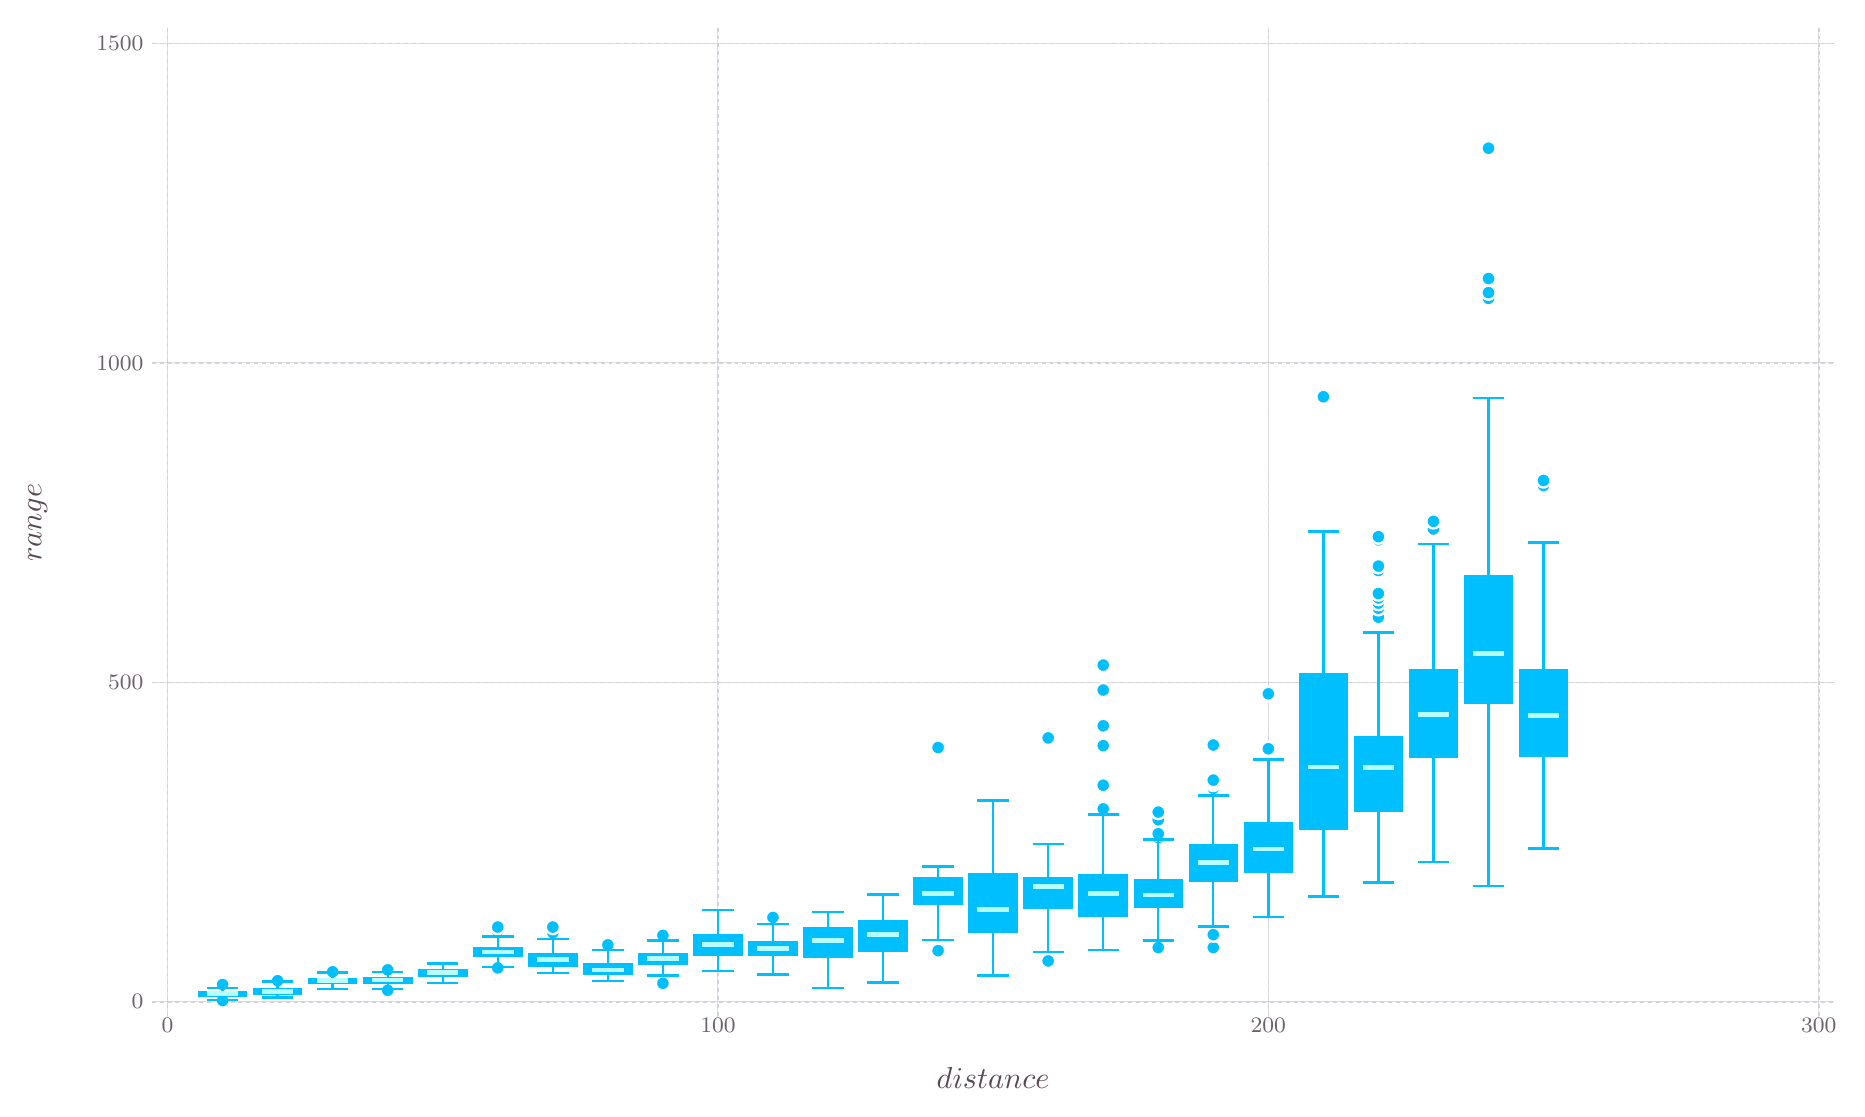
\begin{tikzpicture}[x=1mm,y=-1mm]
\definecolor{mycolorD0D0E0}{rgb}{0.82,0.82,0.88}
\definecolor{mycolor000000}{rgb}{0,0,0}
\definecolor{mycolorB5FFFF}{rgb}{0.71,1,1}
\definecolor{mycolor564A55}{rgb}{0.34,0.29,0.33}
\definecolor{mycolor00BFFF}{rgb}{0,0.75,1}
\definecolor{mycolor000000}{rgb}{0,0,0}
\definecolor{mycolor6C606B}{rgb}{0.42,0.38,0.42}
\definecolor{mycolorFFFFFF}{rgb}{1,1,1}
\begin{scope}
\begin{scope}
\draw (128.15,138.39) node [text=mycolor564A55,draw=mycolor000000,draw opacity=0,rotate around={-0: (0,1.81)},inner sep=0.0]{\fontsize{3.88mm}{4.66mm}\selectfont $\text{distance}$};
\end{scope}
\begin{scope}
\draw (23.31,131.72) node [text=mycolor6C606B,rotate around={-0: (104.85,1.34)},inner sep=0.0]{\fontsize{2.82mm}{3.39mm}\selectfont $\text{0}$};
\draw (93.2,131.72) node [text=mycolor6C606B,rotate around={-0: (34.95,1.34)},inner sep=0.0]{\fontsize{2.82mm}{3.39mm}\selectfont $\text{100}$};
\draw (163.1,131.72) node [text=mycolor6C606B,rotate around={-0: (-34.95,1.34)},inner sep=0.0]{\fontsize{2.82mm}{3.39mm}\selectfont $\text{200}$};
\draw (233,131.72) node [text=mycolor6C606B,rotate around={-0: (-104.85,1.34)},inner sep=0.0]{\fontsize{2.82mm}{3.39mm}\selectfont $\text{300}$};
\end{scope}
\begin{scope}
\clip  (21.31,5) -- (235,5) -- (235,130.72) -- (21.31,130.72);
\begin{scope}
\clip  (21.31,5) -- (235,5) -- (235,130.72) -- (21.31,130.72);
\path [fill=mycolor000000,fill opacity=0,draw=mycolor000000,draw opacity=0] (21.31,5) rectangle +(213.7,125.72);
\end{scope}
\begin{scope}
[dash pattern=on 0.5mm off 0.5mm,line width=0.2mm]
\path [fill=mycolor000000,draw=mycolorD0D0E0]  (21.31,128.71) -- (235,128.71);
\path [fill=mycolor000000,draw=mycolorD0D0E0]  (21.31,88.14) -- (235,88.14);
\path [fill=mycolor000000,draw=mycolorD0D0E0]  (21.31,47.57) -- (235,47.57);
\path [fill=mycolor000000,draw=mycolorD0D0E0]  (21.31,7) -- (235,7);
\end{scope}
\begin{scope}
[dash pattern=on 0.5mm off 0.5mm,line width=0.2mm]
\path [fill=mycolor000000,draw=mycolorD0D0E0]  (23.31,5) -- (23.31,130.72);
\path [fill=mycolor000000,draw=mycolorD0D0E0]  (93.2,5) -- (93.2,130.72);
\path [fill=mycolor000000,draw=mycolorD0D0E0]  (163.1,5) -- (163.1,130.72);
\path [fill=mycolor000000,draw=mycolorD0D0E0]  (233,5) -- (233,130.72);
\end{scope}
\begin{scope}
\begin{scope}
[line width=0.3mm]
\path [fill=mycolor00BFFF,draw=mycolorFFFFFF] (30.29,128.55) circle [radius=0.9];
\path [fill=mycolor00BFFF,draw=mycolorFFFFFF] (30.29,126.85) circle [radius=0.9];
\path [fill=mycolor00BFFF,draw=mycolorFFFFFF] (30.29,126.52) circle [radius=0.9];
\path [fill=mycolor00BFFF,draw=mycolorFFFFFF] (37.28,126.04) circle [radius=0.9];
\path [fill=mycolor00BFFF,draw=mycolorFFFFFF] (44.27,124.9) circle [radius=0.9];
\path [fill=mycolor00BFFF,draw=mycolorFFFFFF] (51.26,127.25) circle [radius=0.9];
\path [fill=mycolor00BFFF,draw=mycolorFFFFFF] (51.26,124.66) circle [radius=0.9];
\path [fill=mycolor00BFFF,draw=mycolorFFFFFF] (51.26,124.66) circle [radius=0.9];
\path [fill=mycolor00BFFF,draw=mycolorFFFFFF] (65.24,125.55) circle [radius=0.9];
\path [fill=mycolor00BFFF,draw=mycolorFFFFFF] (65.24,125.47) circle [radius=0.9];
\path [fill=mycolor00BFFF,draw=mycolorFFFFFF] (65.24,125.39) circle [radius=0.9];
\path [fill=mycolor00BFFF,draw=mycolorFFFFFF] (65.24,125.23) circle [radius=0.9];
\path [fill=mycolor00BFFF,draw=mycolorFFFFFF] (65.24,125.23) circle [radius=0.9];
\path [fill=mycolor00BFFF,draw=mycolorFFFFFF] (65.24,124.9) circle [radius=0.9];
\path [fill=mycolor00BFFF,draw=mycolorFFFFFF] (65.24,124.82) circle [radius=0.9];
\path [fill=mycolor00BFFF,draw=mycolorFFFFFF] (65.24,124.82) circle [radius=0.9];
\path [fill=mycolor00BFFF,draw=mycolorFFFFFF] (65.24,124.82) circle [radius=0.9];
\path [fill=mycolor00BFFF,draw=mycolorFFFFFF] (65.24,124.82) circle [radius=0.9];
\path [fill=mycolor00BFFF,draw=mycolorFFFFFF] (65.24,124.66) circle [radius=0.9];
\path [fill=mycolor00BFFF,draw=mycolorFFFFFF] (65.24,124.66) circle [radius=0.9];
\path [fill=mycolor00BFFF,draw=mycolorFFFFFF] (65.24,124.66) circle [radius=0.9];
\path [fill=mycolor00BFFF,draw=mycolorFFFFFF] (65.24,124.66) circle [radius=0.9];
\path [fill=mycolor00BFFF,draw=mycolorFFFFFF] (65.24,124.66) circle [radius=0.9];
\path [fill=mycolor00BFFF,draw=mycolorFFFFFF] (65.24,124.58) circle [radius=0.9];
\path [fill=mycolor00BFFF,draw=mycolorFFFFFF] (65.24,124.58) circle [radius=0.9];
\path [fill=mycolor00BFFF,draw=mycolorFFFFFF] (65.24,124.41) circle [radius=0.9];
\path [fill=mycolor00BFFF,draw=mycolorFFFFFF] (65.24,120.03) circle [radius=0.9];
\path [fill=mycolor00BFFF,draw=mycolorFFFFFF] (65.24,119.95) circle [radius=0.9];
\path [fill=mycolor00BFFF,draw=mycolorFFFFFF] (65.24,119.71) circle [radius=0.9];
\path [fill=mycolor00BFFF,draw=mycolorFFFFFF] (65.24,119.22) circle [radius=0.9];
\path [fill=mycolor00BFFF,draw=mycolorFFFFFF] (72.23,119.95) circle [radius=0.9];
\path [fill=mycolor00BFFF,draw=mycolorFFFFFF] (72.23,119.22) circle [radius=0.9];
\path [fill=mycolor00BFFF,draw=mycolorFFFFFF] (79.22,121.49) circle [radius=0.9];
\path [fill=mycolor00BFFF,draw=mycolorFFFFFF] (86.21,126.36) circle [radius=0.9];
\path [fill=mycolor00BFFF,draw=mycolorFFFFFF] (86.21,120.52) circle [radius=0.9];
\path [fill=mycolor00BFFF,draw=mycolorFFFFFF] (86.21,120.28) circle [radius=0.9];
\path [fill=mycolor00BFFF,draw=mycolorFFFFFF] (100.19,118.09) circle [radius=0.9];
\path [fill=mycolor00BFFF,draw=mycolorFFFFFF] (100.19,118) circle [radius=0.9];
\path [fill=mycolor00BFFF,draw=mycolorFFFFFF] (121.16,122.22) circle [radius=0.9];
\path [fill=mycolor00BFFF,draw=mycolorFFFFFF] (121.16,96.42) circle [radius=0.9];
\path [fill=mycolor00BFFF,draw=mycolorFFFFFF] (135.14,123.52) circle [radius=0.9];
\path [fill=mycolor00BFFF,draw=mycolorFFFFFF] (135.14,95.2) circle [radius=0.9];
\path [fill=mycolor00BFFF,draw=mycolorFFFFFF] (142.13,104.37) circle [radius=0.9];
\path [fill=mycolor00BFFF,draw=mycolorFFFFFF] (142.13,104.21) circle [radius=0.9];
\path [fill=mycolor00BFFF,draw=mycolorFFFFFF] (142.13,101.21) circle [radius=0.9];
\path [fill=mycolor00BFFF,draw=mycolorFFFFFF] (142.13,96.18) circle [radius=0.9];
\path [fill=mycolor00BFFF,draw=mycolorFFFFFF] (142.13,93.66) circle [radius=0.9];
\path [fill=mycolor00BFFF,draw=mycolorFFFFFF] (142.13,89.12) circle [radius=0.9];
\path [fill=mycolor00BFFF,draw=mycolorFFFFFF] (142.13,85.95) circle [radius=0.9];
\path [fill=mycolor00BFFF,draw=mycolorFFFFFF] (149.12,121.82) circle [radius=0.9];
\path [fill=mycolor00BFFF,draw=mycolorFFFFFF] (149.12,107.86) circle [radius=0.9];
\path [fill=mycolor00BFFF,draw=mycolorFFFFFF] (149.12,107.37) circle [radius=0.9];
\path [fill=mycolor00BFFF,draw=mycolorFFFFFF] (149.12,105.59) circle [radius=0.9];
\path [fill=mycolor00BFFF,draw=mycolorFFFFFF] (149.12,104.62) circle [radius=0.9];
\path [fill=mycolor00BFFF,draw=mycolorFFFFFF] (156.11,121.82) circle [radius=0.9];
\path [fill=mycolor00BFFF,draw=mycolorFFFFFF] (156.11,120.19) circle [radius=0.9];
\path [fill=mycolor00BFFF,draw=mycolorFFFFFF] (156.11,101.86) circle [radius=0.9];
\path [fill=mycolor00BFFF,draw=mycolorFFFFFF] (156.11,101.61) circle [radius=0.9];
\path [fill=mycolor00BFFF,draw=mycolorFFFFFF] (156.11,101.05) circle [radius=0.9];
\path [fill=mycolor00BFFF,draw=mycolorFFFFFF] (156.11,100.88) circle [radius=0.9];
\path [fill=mycolor00BFFF,draw=mycolorFFFFFF] (156.11,100.8) circle [radius=0.9];
\path [fill=mycolor00BFFF,draw=mycolorFFFFFF] (156.11,100.56) circle [radius=0.9];
\path [fill=mycolor00BFFF,draw=mycolorFFFFFF] (156.11,96.1) circle [radius=0.9];
\path [fill=mycolor00BFFF,draw=mycolorFFFFFF] (163.1,96.58) circle [radius=0.9];
\path [fill=mycolor00BFFF,draw=mycolorFFFFFF] (163.1,89.6) circle [radius=0.9];
\path [fill=mycolor00BFFF,draw=mycolorFFFFFF] (170.09,51.87) circle [radius=0.9];
\path [fill=mycolor00BFFF,draw=mycolorFFFFFF] (177.08,79.87) circle [radius=0.9];
\path [fill=mycolor00BFFF,draw=mycolorFFFFFF] (177.08,78.73) circle [radius=0.9];
\path [fill=mycolor00BFFF,draw=mycolorFFFFFF] (177.08,78.08) circle [radius=0.9];
\path [fill=mycolor00BFFF,draw=mycolorFFFFFF] (177.08,77.43) circle [radius=0.9];
\path [fill=mycolor00BFFF,draw=mycolorFFFFFF] (177.08,76.86) circle [radius=0.9];
\path [fill=mycolor00BFFF,draw=mycolorFFFFFF] (177.08,73.94) circle [radius=0.9];
\path [fill=mycolor00BFFF,draw=mycolorFFFFFF] (177.08,73.38) circle [radius=0.9];
\path [fill=mycolor00BFFF,draw=mycolorFFFFFF] (177.08,73.38) circle [radius=0.9];
\path [fill=mycolor00BFFF,draw=mycolorFFFFFF] (177.08,70.05) circle [radius=0.9];
\path [fill=mycolor00BFFF,draw=mycolorFFFFFF] (177.08,69.64) circle [radius=0.9];
\path [fill=mycolor00BFFF,draw=mycolorFFFFFF] (184.07,68.83) circle [radius=0.9];
\path [fill=mycolor00BFFF,draw=mycolorFFFFFF] (184.07,68.67) circle [radius=0.9];
\path [fill=mycolor00BFFF,draw=mycolorFFFFFF] (184.07,67.7) circle [radius=0.9];
\path [fill=mycolor00BFFF,draw=mycolorFFFFFF] (191.06,39.38) circle [radius=0.9];
\path [fill=mycolor00BFFF,draw=mycolorFFFFFF] (191.06,38.65) circle [radius=0.9];
\path [fill=mycolor00BFFF,draw=mycolorFFFFFF] (191.06,36.86) circle [radius=0.9];
\path [fill=mycolor00BFFF,draw=mycolorFFFFFF] (191.06,20.31) circle [radius=0.9];
\path [fill=mycolor00BFFF,draw=mycolorFFFFFF] (198.05,63.15) circle [radius=0.9];
\path [fill=mycolor00BFFF,draw=mycolorFFFFFF] (198.05,62.5) circle [radius=0.9];
\path [fill=mycolor00BFFF,draw=mycolor00BFFF] (27.3,127.5) rectangle +(5.99,0.41);
\path [fill=mycolor00BFFF,draw=mycolor00BFFF] (34.29,127.09) rectangle +(5.99,0.65);
\path [fill=mycolor00BFFF,draw=mycolor00BFFF] (41.28,125.79) rectangle +(5.99,0.57);
\path [fill=mycolor00BFFF,draw=mycolor00BFFF] (48.27,125.71) rectangle +(5.99,0.57);
\path [fill=mycolor00BFFF,draw=mycolor00BFFF] (55.26,124.66) rectangle +(5.99,0.73);
\path [fill=mycolor00BFFF,draw=mycolor00BFFF] (62.25,121.88) rectangle +(5.99,0.99);
\path [fill=mycolor00BFFF,draw=mycolor00BFFF] (69.24,122.71) rectangle +(5.99,1.38);
\path [fill=mycolor00BFFF,draw=mycolor00BFFF] (76.23,123.93) rectangle +(5.99,1.22);
\path [fill=mycolor00BFFF,draw=mycolor00BFFF] (83.22,122.63) rectangle +(5.99,1.3);
\path [fill=mycolor00BFFF,draw=mycolor00BFFF] (90.21,120.19) rectangle +(5.99,2.54);
\path [fill=mycolor00BFFF,draw=mycolor00BFFF] (97.2,121.17) rectangle +(5.99,1.62);
\path [fill=mycolor00BFFF,draw=mycolor00BFFF] (104.19,119.38) rectangle +(5.99,3.57);
\path [fill=mycolor00BFFF,draw=mycolor00BFFF] (111.18,118.49) rectangle +(5.99,3.75);
\path [fill=mycolor00BFFF,draw=mycolor00BFFF] (118.17,113.05) rectangle +(5.99,3.21);
\path [fill=mycolor00BFFF,draw=mycolor00BFFF] (125.16,112.45) rectangle +(5.99,7.34);
\path [fill=mycolor00BFFF,draw=mycolor00BFFF] (132.15,112.97) rectangle +(5.99,3.77);
\path [fill=mycolor00BFFF,draw=mycolor00BFFF] (139.14,112.63) rectangle +(5.99,5.13);
\path [fill=mycolor00BFFF,draw=mycolor00BFFF] (146.13,113.22) rectangle +(5.99,3.41);
\path [fill=mycolor00BFFF,draw=mycolor00BFFF] (153.12,108.88) rectangle +(5.99,4.5);
\path [fill=mycolor00BFFF,draw=mycolor00BFFF] (160.11,106.06) rectangle +(5.99,6.19);
\path [fill=mycolor00BFFF,draw=mycolor00BFFF] (167.1,87.11) rectangle +(5.99,19.62);
\path [fill=mycolor00BFFF,draw=mycolor00BFFF] (174.09,95.08) rectangle +(5.99,9.39);
\path [fill=mycolor00BFFF,draw=mycolor00BFFF] (181.08,86.64) rectangle +(5.99,10.95);
\path [fill=mycolor00BFFF,draw=mycolor00BFFF] (188.07,74.61) rectangle +(5.99,16.15);
\path [fill=mycolor00BFFF,draw=mycolor00BFFF] (195.06,86.6) rectangle +(5.99,10.87);
\path [fill=mycolor00BFFF,draw=mycolor00BFFF]  (28.3,126.93) -- (32.29,126.93);
\path [fill=mycolor00BFFF,draw=mycolor00BFFF]  (35.29,126.12) -- (39.28,126.12);
\path [fill=mycolor00BFFF,draw=mycolor00BFFF]  (42.28,124.98) -- (46.27,124.98);
\path [fill=mycolor00BFFF,draw=mycolor00BFFF]  (49.27,124.9) -- (53.26,124.9);
\path [fill=mycolor00BFFF,draw=mycolor00BFFF]  (56.26,123.85) -- (60.25,123.85);
\path [fill=mycolor00BFFF,draw=mycolor00BFFF]  (63.25,120.44) -- (67.24,120.44);
\path [fill=mycolor00BFFF,draw=mycolor00BFFF]  (70.24,120.76) -- (74.23,120.76);
\path [fill=mycolor00BFFF,draw=mycolor00BFFF]  (77.23,122.14) -- (81.22,122.14);
\path [fill=mycolor00BFFF,draw=mycolor00BFFF]  (84.22,120.93) -- (88.21,120.93);
\path [fill=mycolor00BFFF,draw=mycolor00BFFF]  (91.21,117.03) -- (95.2,117.03);
\path [fill=mycolor00BFFF,draw=mycolor00BFFF]  (98.2,118.82) -- (102.19,118.82);
\path [fill=mycolor00BFFF,draw=mycolor00BFFF]  (105.19,117.27) -- (109.18,117.27);
\path [fill=mycolor00BFFF,draw=mycolor00BFFF]  (112.18,115.08) -- (116.17,115.08);
\path [fill=mycolor00BFFF,draw=mycolor00BFFF]  (119.17,111.51) -- (123.16,111.51);
\path [fill=mycolor00BFFF,draw=mycolor00BFFF]  (126.16,103.15) -- (130.15,103.15);
\path [fill=mycolor00BFFF,draw=mycolor00BFFF]  (133.15,108.67) -- (137.14,108.67);
\path [fill=mycolor00BFFF,draw=mycolor00BFFF]  (140.14,104.94) -- (144.13,104.94);
\path [fill=mycolor00BFFF,draw=mycolor00BFFF]  (147.13,108.1) -- (151.12,108.1);
\path [fill=mycolor00BFFF,draw=mycolor00BFFF]  (154.12,102.51) -- (158.11,102.51);
\path [fill=mycolor00BFFF,draw=mycolor00BFFF]  (161.11,97.96) -- (165.1,97.96);
\path [fill=mycolor00BFFF,draw=mycolor00BFFF]  (168.09,68.99) -- (172.09,68.99);
\path [fill=mycolor00BFFF,draw=mycolor00BFFF]  (175.08,81.81) -- (179.08,81.81);
\path [fill=mycolor00BFFF,draw=mycolor00BFFF]  (182.07,70.54) -- (186.07,70.54);
\path [fill=mycolor00BFFF,draw=mycolor00BFFF]  (189.06,52.03) -- (193.06,52.03);
\path [fill=mycolor00BFFF,draw=mycolor00BFFF]  (196.05,70.37) -- (200.05,70.37);
\path [fill=mycolor00BFFF,draw=mycolor00BFFF]  (28.3,128.47) -- (32.29,128.47);
\path [fill=mycolor00BFFF,draw=mycolor00BFFF]  (35.29,128.15) -- (39.28,128.15);
\path [fill=mycolor00BFFF,draw=mycolor00BFFF]  (42.28,127.09) -- (46.27,127.09);
\path [fill=mycolor00BFFF,draw=mycolor00BFFF]  (49.27,127.09) -- (53.26,127.09);
\path [fill=mycolor00BFFF,draw=mycolor00BFFF]  (56.26,126.36) -- (60.25,126.36);
\path [fill=mycolor00BFFF,draw=mycolor00BFFF]  (63.25,124.33) -- (67.24,124.33);
\path [fill=mycolor00BFFF,draw=mycolor00BFFF]  (70.24,125.06) -- (74.23,125.06);
\path [fill=mycolor00BFFF,draw=mycolor00BFFF]  (77.23,126.04) -- (81.22,126.04);
\path [fill=mycolor00BFFF,draw=mycolor00BFFF]  (84.22,125.39) -- (88.21,125.39);
\path [fill=mycolor00BFFF,draw=mycolor00BFFF]  (91.21,124.82) -- (95.2,124.82);
\path [fill=mycolor00BFFF,draw=mycolor00BFFF]  (98.2,125.23) -- (102.19,125.23);
\path [fill=mycolor00BFFF,draw=mycolor00BFFF]  (105.19,126.93) -- (109.18,126.93);
\path [fill=mycolor00BFFF,draw=mycolor00BFFF]  (112.18,126.28) -- (116.17,126.28);
\path [fill=mycolor00BFFF,draw=mycolor00BFFF]  (119.17,120.84) -- (123.16,120.84);
\path [fill=mycolor00BFFF,draw=mycolor00BFFF]  (126.16,125.39) -- (130.15,125.39);
\path [fill=mycolor00BFFF,draw=mycolor00BFFF]  (133.15,122.39) -- (137.14,122.39);
\path [fill=mycolor00BFFF,draw=mycolor00BFFF]  (140.14,122.14) -- (144.13,122.14);
\path [fill=mycolor00BFFF,draw=mycolor00BFFF]  (147.13,120.93) -- (151.12,120.93);
\path [fill=mycolor00BFFF,draw=mycolor00BFFF]  (154.12,119.14) -- (158.11,119.14);
\path [fill=mycolor00BFFF,draw=mycolor00BFFF]  (161.11,117.92) -- (165.1,117.92);
\path [fill=mycolor00BFFF,draw=mycolor00BFFF]  (168.09,115.33) -- (172.09,115.33);
\path [fill=mycolor00BFFF,draw=mycolor00BFFF]  (175.08,113.54) -- (179.08,113.54);
\path [fill=mycolor00BFFF,draw=mycolor00BFFF]  (182.07,110.94) -- (186.07,110.94);
\path [fill=mycolor00BFFF,draw=mycolor00BFFF]  (189.06,114.03) -- (193.06,114.03);
\path [fill=mycolor00BFFF,draw=mycolor00BFFF]  (196.05,109.24) -- (200.05,109.24);
\path [fill=mycolor00BFFF,draw=mycolor00BFFF]  (30.29,127.5) -- (30.29,126.93);
\path [fill=mycolor00BFFF,draw=mycolor00BFFF]  (37.28,127.09) -- (37.28,126.12);
\path [fill=mycolor00BFFF,draw=mycolor00BFFF]  (44.27,125.79) -- (44.27,124.98);
\path [fill=mycolor00BFFF,draw=mycolor00BFFF]  (51.26,125.71) -- (51.26,124.9);
\path [fill=mycolor00BFFF,draw=mycolor00BFFF]  (58.25,124.66) -- (58.25,123.85);
\path [fill=mycolor00BFFF,draw=mycolor00BFFF]  (65.24,121.88) -- (65.24,120.44);
\path [fill=mycolor00BFFF,draw=mycolor00BFFF]  (72.23,122.71) -- (72.23,120.76);
\path [fill=mycolor00BFFF,draw=mycolor00BFFF]  (79.22,123.93) -- (79.22,122.14);
\path [fill=mycolor00BFFF,draw=mycolor00BFFF]  (86.21,122.63) -- (86.21,120.93);
\path [fill=mycolor00BFFF,draw=mycolor00BFFF]  (93.2,120.19) -- (93.2,117.03);
\path [fill=mycolor00BFFF,draw=mycolor00BFFF]  (100.19,121.17) -- (100.19,118.82);
\path [fill=mycolor00BFFF,draw=mycolor00BFFF]  (107.18,119.38) -- (107.18,117.27);
\path [fill=mycolor00BFFF,draw=mycolor00BFFF]  (114.17,118.49) -- (114.17,115.08);
\path [fill=mycolor00BFFF,draw=mycolor00BFFF]  (121.16,113.05) -- (121.16,111.51);
\path [fill=mycolor00BFFF,draw=mycolor00BFFF]  (128.15,112.45) -- (128.15,103.15);
\path [fill=mycolor00BFFF,draw=mycolor00BFFF]  (135.14,112.97) -- (135.14,108.67);
\path [fill=mycolor00BFFF,draw=mycolor00BFFF]  (142.13,112.63) -- (142.13,104.94);
\path [fill=mycolor00BFFF,draw=mycolor00BFFF]  (149.12,113.22) -- (149.12,108.1);
\path [fill=mycolor00BFFF,draw=mycolor00BFFF]  (156.11,108.88) -- (156.11,102.51);
\path [fill=mycolor00BFFF,draw=mycolor00BFFF]  (163.1,106.06) -- (163.1,97.96);
\path [fill=mycolor00BFFF,draw=mycolor00BFFF]  (170.09,87.11) -- (170.09,68.99);
\path [fill=mycolor00BFFF,draw=mycolor00BFFF]  (177.08,95.08) -- (177.08,81.81);
\path [fill=mycolor00BFFF,draw=mycolor00BFFF]  (184.07,86.64) -- (184.07,70.54);
\path [fill=mycolor00BFFF,draw=mycolor00BFFF]  (191.06,74.61) -- (191.06,52.03);
\path [fill=mycolor00BFFF,draw=mycolor00BFFF]  (198.05,86.6) -- (198.05,70.37);
\path [fill=mycolor00BFFF,draw=mycolor00BFFF]  (30.29,127.9) -- (30.29,128.47);
\path [fill=mycolor00BFFF,draw=mycolor00BFFF]  (37.28,127.74) -- (37.28,128.15);
\path [fill=mycolor00BFFF,draw=mycolor00BFFF]  (44.27,126.36) -- (44.27,127.09);
\path [fill=mycolor00BFFF,draw=mycolor00BFFF]  (51.26,126.28) -- (51.26,127.09);
\path [fill=mycolor00BFFF,draw=mycolor00BFFF]  (58.25,125.39) -- (58.25,126.36);
\path [fill=mycolor00BFFF,draw=mycolor00BFFF]  (65.24,122.87) -- (65.24,124.33);
\path [fill=mycolor00BFFF,draw=mycolor00BFFF]  (72.23,124.09) -- (72.23,125.06);
\path [fill=mycolor00BFFF,draw=mycolor00BFFF]  (79.22,125.14) -- (79.22,126.04);
\path [fill=mycolor00BFFF,draw=mycolor00BFFF]  (86.21,123.93) -- (86.21,125.39);
\path [fill=mycolor00BFFF,draw=mycolor00BFFF]  (93.2,122.73) -- (93.2,124.82);
\path [fill=mycolor00BFFF,draw=mycolor00BFFF]  (100.19,122.79) -- (100.19,125.23);
\path [fill=mycolor00BFFF,draw=mycolor00BFFF]  (107.18,122.95) -- (107.18,126.93);
\path [fill=mycolor00BFFF,draw=mycolor00BFFF]  (114.17,122.24) -- (114.17,126.28);
\path [fill=mycolor00BFFF,draw=mycolor00BFFF]  (121.16,116.26) -- (121.16,120.84);
\path [fill=mycolor00BFFF,draw=mycolor00BFFF]  (128.15,119.79) -- (128.15,125.39);
\path [fill=mycolor00BFFF,draw=mycolor00BFFF]  (135.14,116.75) -- (135.14,122.39);
\path [fill=mycolor00BFFF,draw=mycolor00BFFF]  (142.13,117.76) -- (142.13,122.14);
\path [fill=mycolor00BFFF,draw=mycolor00BFFF]  (149.12,116.62) -- (149.12,120.93);
\path [fill=mycolor00BFFF,draw=mycolor00BFFF]  (156.11,113.38) -- (156.11,119.14);
\path [fill=mycolor00BFFF,draw=mycolor00BFFF]  (163.1,112.24) -- (163.1,117.92);
\path [fill=mycolor00BFFF,draw=mycolor00BFFF]  (170.09,106.73) -- (170.09,115.33);
\path [fill=mycolor00BFFF,draw=mycolor00BFFF]  (177.08,104.47) -- (177.08,113.54);
\path [fill=mycolor00BFFF,draw=mycolor00BFFF]  (184.07,97.6) -- (184.07,110.94);
\path [fill=mycolor00BFFF,draw=mycolor00BFFF]  (191.06,90.76) -- (191.06,114.03);
\path [fill=mycolor00BFFF,draw=mycolor00BFFF]  (198.05,97.47) -- (198.05,109.24);
\begin{scope}
[line width=0.6mm]
\path [fill=mycolor00BFFF,draw=mycolorB5FFFF]  (28.3,127.7) -- (32.29,127.7);
\path [fill=mycolor00BFFF,draw=mycolorB5FFFF]  (35.29,127.42) -- (39.28,127.42);
\path [fill=mycolor00BFFF,draw=mycolorB5FFFF]  (42.28,126.04) -- (46.27,126.04);
\path [fill=mycolor00BFFF,draw=mycolorB5FFFF]  (49.27,125.96) -- (53.26,125.96);
\path [fill=mycolor00BFFF,draw=mycolorB5FFFF]  (56.26,124.98) -- (60.25,124.98);
\path [fill=mycolor00BFFF,draw=mycolorB5FFFF]  (63.25,122.39) -- (67.24,122.39);
\path [fill=mycolor00BFFF,draw=mycolorB5FFFF]  (70.24,123.36) -- (74.23,123.36);
\path [fill=mycolor00BFFF,draw=mycolorB5FFFF]  (77.23,124.66) -- (81.22,124.66);
\path [fill=mycolor00BFFF,draw=mycolorB5FFFF]  (84.22,123.2) -- (88.21,123.2);
\path [fill=mycolor00BFFF,draw=mycolorB5FFFF]  (91.21,121.41) -- (95.2,121.41);
\path [fill=mycolor00BFFF,draw=mycolorB5FFFF]  (98.2,121.98) -- (102.19,121.98);
\path [fill=mycolor00BFFF,draw=mycolorB5FFFF]  (105.19,120.93) -- (109.18,120.93);
\path [fill=mycolor00BFFF,draw=mycolorB5FFFF]  (112.18,120.19) -- (116.17,120.19);
\path [fill=mycolor00BFFF,draw=mycolorB5FFFF]  (119.17,114.92) -- (123.16,114.92);
\path [fill=mycolor00BFFF,draw=mycolorB5FFFF]  (126.16,116.99) -- (130.15,116.99);
\path [fill=mycolor00BFFF,draw=mycolorB5FFFF]  (133.15,114.11) -- (137.14,114.11);
\path [fill=mycolor00BFFF,draw=mycolorB5FFFF]  (140.14,115) -- (144.13,115);
\path [fill=mycolor00BFFF,draw=mycolorB5FFFF]  (147.13,115.16) -- (151.12,115.16);
\path [fill=mycolor00BFFF,draw=mycolorB5FFFF]  (154.12,111.03) -- (158.11,111.03);
\path [fill=mycolor00BFFF,draw=mycolorB5FFFF]  (161.11,109.32) -- (165.1,109.32);
\path [fill=mycolor00BFFF,draw=mycolorB5FFFF]  (168.09,98.89) -- (172.09,98.89);
\path [fill=mycolor00BFFF,draw=mycolorB5FFFF]  (175.08,98.94) -- (179.08,98.94);
\path [fill=mycolor00BFFF,draw=mycolorB5FFFF]  (182.07,92.2) -- (186.07,92.2);
\path [fill=mycolor00BFFF,draw=mycolorB5FFFF]  (189.06,84.45) -- (193.06,84.45);
\path [fill=mycolor00BFFF,draw=mycolorB5FFFF]  (196.05,92.32) -- (200.05,92.32);
\end{scope}
\end{scope}
\end{scope}
\end{scope}
\begin{scope}
\draw (20.31,128.71) node [text=mycolor6C606B,rotate around={-0: (-3.35,-60.86)},left,inner sep=0.0]{\fontsize{2.82mm}{3.39mm}\selectfont $\text{0}$};
\draw (20.31,88.14) node [text=mycolor6C606B,rotate around={-0: (-3.35,-20.29)},left,inner sep=0.0]{\fontsize{2.82mm}{3.39mm}\selectfont $\text{500}$};
\draw (20.31,47.57) node [text=mycolor6C606B,rotate around={-0: (-3.35,20.29)},left,inner sep=0.0]{\fontsize{2.82mm}{3.39mm}\selectfont $\text{1000}$};
\draw (20.31,7) node [text=mycolor6C606B,rotate around={-0: (-3.35,60.86)},left,inner sep=0.0]{\fontsize{2.82mm}{3.39mm}\selectfont $\text{1500}$};
\end{scope}
\begin{scope}
\draw (8.81,65.86) node [text=mycolor564A55,draw=mycolor000000,draw opacity=0,rotate around={90: (0,2)},inner sep=0.0]{\fontsize{3.88mm}{4.66mm}\selectfont $\text{range}$};
\end{scope}
\end{scope}
\end{tikzpicture}

%		\caption{range values and real distance}
%		\label{boxplot}
%	\end{figure}
%
%	\begin{figure}[h]
%		\centering
%		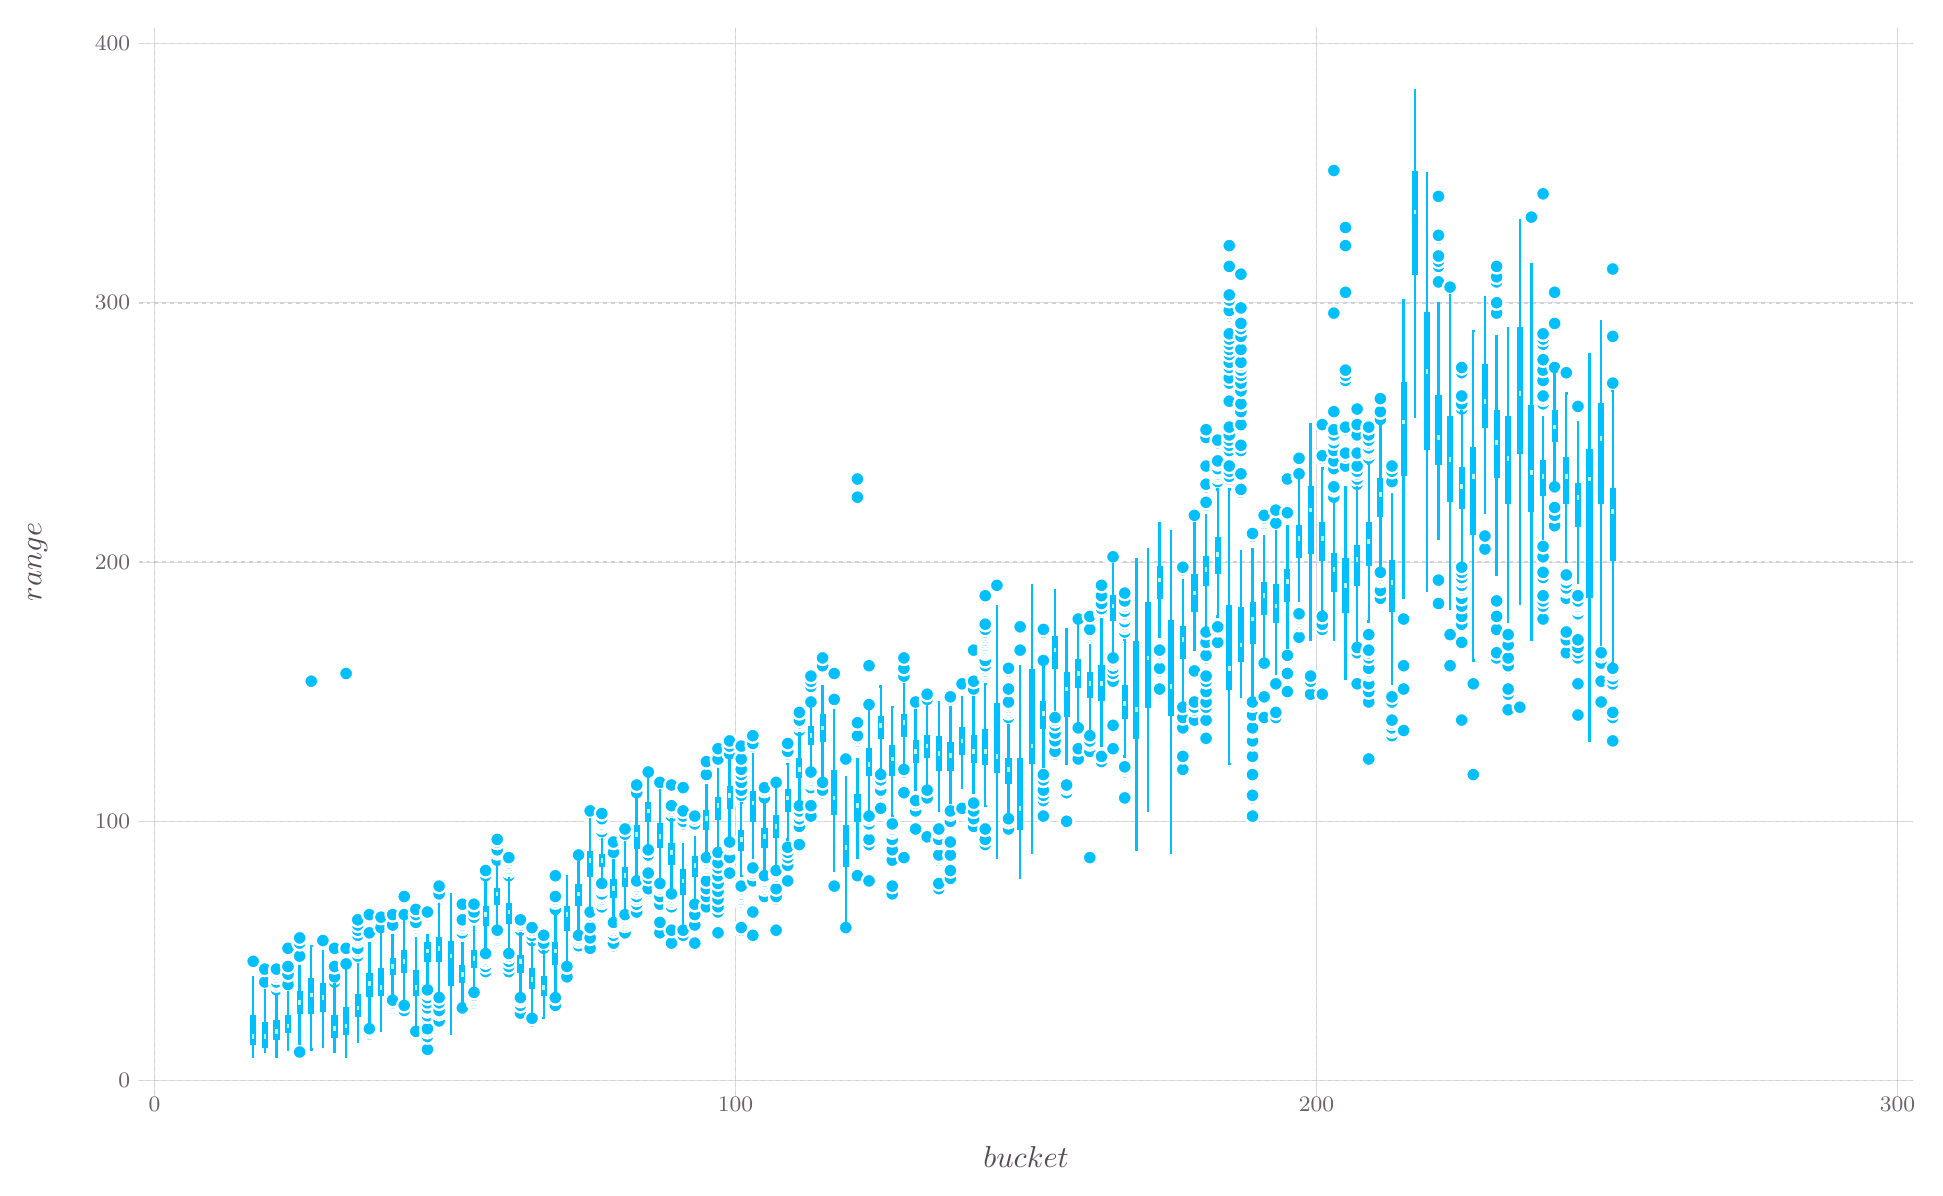
\begin{tikzpicture}[x=1mm,y=-1mm]
\definecolor{mycolorD0D0E0}{rgb}{0.82,0.82,0.88}
\definecolor{mycolorFFFFFF}{rgb}{1,1,1}
\definecolor{mycolor000000}{rgb}{0,0,0}
\definecolor{mycolor000000}{rgb}{0,0,0}
\definecolor{mycolor00BFFF}{rgb}{0,0.75,1}
\definecolor{mycolor564A55}{rgb}{0.34,0.29,0.33}
\definecolor{mycolor6C606B}{rgb}{0.42,0.38,0.42}
\definecolor{mycolorB5FFFF}{rgb}{0.71,1,1}
\begin{scope}
\begin{scope}
\draw (132.32,148.39) node [text=mycolor564A55,draw=mycolor000000,draw opacity=0,rotate around={-0: (0,1.81)},inner sep=0.0]{\fontsize{3.88mm}{4.66mm}\selectfont $\text{bucket}$};
\end{scope}
\begin{scope}
\draw (21.63,141.72) node [text=mycolor6C606B,rotate around={-0: (110.68,1.34)},inner sep=0.0]{\fontsize{2.82mm}{3.39mm}\selectfont $\text{0}$};
\draw (95.42,141.72) node [text=mycolor6C606B,rotate around={-0: (36.89,1.34)},inner sep=0.0]{\fontsize{2.82mm}{3.39mm}\selectfont $\text{100}$};
\draw (169.21,141.72) node [text=mycolor6C606B,rotate around={-0: (-36.89,1.34)},inner sep=0.0]{\fontsize{2.82mm}{3.39mm}\selectfont $\text{200}$};
\draw (243,141.72) node [text=mycolor6C606B,rotate around={-0: (-110.68,1.34)},inner sep=0.0]{\fontsize{2.82mm}{3.39mm}\selectfont $\text{300}$};
\end{scope}
\begin{scope}
\clip  (19.63,5) -- (245,5) -- (245,140.72) -- (19.63,140.72);
\begin{scope}
\clip  (19.63,5) -- (245,5) -- (245,140.72) -- (19.63,140.72);
\path [fill=mycolor000000,fill opacity=0,draw=mycolor000000,draw opacity=0] (19.63,5) rectangle +(225.37,135.72);
\end{scope}
\begin{scope}
[dash pattern=on 0.5mm off 0.5mm,line width=0.2mm]
\path [fill=mycolor000000,draw=mycolorD0D0E0]  (19.63,138.72) -- (245,138.72);
\path [fill=mycolor000000,draw=mycolorD0D0E0]  (19.63,105.79) -- (245,105.79);
\path [fill=mycolor000000,draw=mycolorD0D0E0]  (19.63,72.86) -- (245,72.86);
\path [fill=mycolor000000,draw=mycolorD0D0E0]  (19.63,39.93) -- (245,39.93);
\path [fill=mycolor000000,draw=mycolorD0D0E0]  (19.63,7) -- (245,7);
\end{scope}
\begin{scope}
[dash pattern=on 0.5mm off 0.5mm,line width=0.2mm]
\path [fill=mycolor000000,draw=mycolorD0D0E0]  (21.63,5) -- (21.63,140.72);
\path [fill=mycolor000000,draw=mycolorD0D0E0]  (95.42,5) -- (95.42,140.72);
\path [fill=mycolor000000,draw=mycolorD0D0E0]  (169.21,5) -- (169.21,140.72);
\path [fill=mycolor000000,draw=mycolorD0D0E0]  (243,5) -- (243,140.72);
\end{scope}
\begin{scope}
\begin{scope}
[line width=0.3mm]
\path [fill=mycolor00BFFF,draw=mycolorFFFFFF] (34.18,123.57) circle [radius=0.9];
\path [fill=mycolor00BFFF,draw=mycolorFFFFFF] (35.65,126.2) circle [radius=0.9];
\path [fill=mycolor00BFFF,draw=mycolorFFFFFF] (35.65,126.2) circle [radius=0.9];
\path [fill=mycolor00BFFF,draw=mycolorFFFFFF] (35.65,126.2) circle [radius=0.9];
\path [fill=mycolor00BFFF,draw=mycolorFFFFFF] (35.65,124.56) circle [radius=0.9];
\path [fill=mycolor00BFFF,draw=mycolorFFFFFF] (37.13,127.52) circle [radius=0.9];
\path [fill=mycolor00BFFF,draw=mycolorFFFFFF] (37.13,127.52) circle [radius=0.9];
\path [fill=mycolor00BFFF,draw=mycolorFFFFFF] (37.13,127.19) circle [radius=0.9];
\path [fill=mycolor00BFFF,draw=mycolorFFFFFF] (37.13,127.19) circle [radius=0.9];
\path [fill=mycolor00BFFF,draw=mycolorFFFFFF] (37.13,127.19) circle [radius=0.9];
\path [fill=mycolor00BFFF,draw=mycolorFFFFFF] (37.13,127.19) circle [radius=0.9];
\path [fill=mycolor00BFFF,draw=mycolorFFFFFF] (37.13,126.53) circle [radius=0.9];
\path [fill=mycolor00BFFF,draw=mycolorFFFFFF] (37.13,126.2) circle [radius=0.9];
\path [fill=mycolor00BFFF,draw=mycolorFFFFFF] (37.13,126.2) circle [radius=0.9];
\path [fill=mycolor00BFFF,draw=mycolorFFFFFF] (37.13,126.2) circle [radius=0.9];
\path [fill=mycolor00BFFF,draw=mycolorFFFFFF] (37.13,125.54) circle [radius=0.9];
\path [fill=mycolor00BFFF,draw=mycolorFFFFFF] (37.13,125.54) circle [radius=0.9];
\path [fill=mycolor00BFFF,draw=mycolorFFFFFF] (37.13,125.21) circle [radius=0.9];
\path [fill=mycolor00BFFF,draw=mycolorFFFFFF] (37.13,125.21) circle [radius=0.9];
\path [fill=mycolor00BFFF,draw=mycolorFFFFFF] (37.13,124.88) circle [radius=0.9];
\path [fill=mycolor00BFFF,draw=mycolorFFFFFF] (37.13,124.56) circle [radius=0.9];
\path [fill=mycolor00BFFF,draw=mycolorFFFFFF] (38.6,127.19) circle [radius=0.9];
\path [fill=mycolor00BFFF,draw=mycolorFFFFFF] (38.6,126.86) circle [radius=0.9];
\path [fill=mycolor00BFFF,draw=mycolorFFFFFF] (38.6,126.53) circle [radius=0.9];
\path [fill=mycolor00BFFF,draw=mycolorFFFFFF] (38.6,126.53) circle [radius=0.9];
\path [fill=mycolor00BFFF,draw=mycolorFFFFFF] (38.6,125.21) circle [radius=0.9];
\path [fill=mycolor00BFFF,draw=mycolorFFFFFF] (38.6,125.21) circle [radius=0.9];
\path [fill=mycolor00BFFF,draw=mycolorFFFFFF] (38.6,124.23) circle [radius=0.9];
\path [fill=mycolor00BFFF,draw=mycolorFFFFFF] (38.6,121.92) circle [radius=0.9];
\path [fill=mycolor00BFFF,draw=mycolorFFFFFF] (40.08,135.09) circle [radius=0.9];
\path [fill=mycolor00BFFF,draw=mycolorFFFFFF] (40.08,123.24) circle [radius=0.9];
\path [fill=mycolor00BFFF,draw=mycolorFFFFFF] (40.08,123.24) circle [radius=0.9];
\path [fill=mycolor00BFFF,draw=mycolorFFFFFF] (40.08,122.91) circle [radius=0.9];
\path [fill=mycolor00BFFF,draw=mycolorFFFFFF] (40.08,122.91) circle [radius=0.9];
\path [fill=mycolor00BFFF,draw=mycolorFFFFFF] (40.08,121.26) circle [radius=0.9];
\path [fill=mycolor00BFFF,draw=mycolorFFFFFF] (40.08,121.26) circle [radius=0.9];
\path [fill=mycolor00BFFF,draw=mycolorFFFFFF] (40.08,121.26) circle [radius=0.9];
\path [fill=mycolor00BFFF,draw=mycolorFFFFFF] (40.08,120.6) circle [radius=0.9];
\path [fill=mycolor00BFFF,draw=mycolorFFFFFF] (41.55,88) circle [radius=0.9];
\path [fill=mycolor00BFFF,draw=mycolorFFFFFF] (43.03,120.93) circle [radius=0.9];
\path [fill=mycolor00BFFF,draw=mycolorFFFFFF] (44.51,126.2) circle [radius=0.9];
\path [fill=mycolor00BFFF,draw=mycolorFFFFFF] (44.51,125.54) circle [radius=0.9];
\path [fill=mycolor00BFFF,draw=mycolorFFFFFF] (44.51,124.23) circle [radius=0.9];
\path [fill=mycolor00BFFF,draw=mycolorFFFFFF] (44.51,121.92) circle [radius=0.9];
\path [fill=mycolor00BFFF,draw=mycolorFFFFFF] (45.98,124.23) circle [radius=0.9];
\path [fill=mycolor00BFFF,draw=mycolorFFFFFF] (45.98,124.23) circle [radius=0.9];
\path [fill=mycolor00BFFF,draw=mycolorFFFFFF] (45.98,123.9) circle [radius=0.9];
\path [fill=mycolor00BFFF,draw=mycolorFFFFFF] (45.98,123.9) circle [radius=0.9];
\path [fill=mycolor00BFFF,draw=mycolorFFFFFF] (45.98,121.92) circle [radius=0.9];
\path [fill=mycolor00BFFF,draw=mycolorFFFFFF] (45.98,87.02) circle [radius=0.9];
\path [fill=mycolor00BFFF,draw=mycolorFFFFFF] (47.46,122.91) circle [radius=0.9];
\path [fill=mycolor00BFFF,draw=mycolorFFFFFF] (47.46,122.25) circle [radius=0.9];
\path [fill=mycolor00BFFF,draw=mycolorFFFFFF] (47.46,121.92) circle [radius=0.9];
\path [fill=mycolor00BFFF,draw=mycolorFFFFFF] (47.46,120.93) circle [radius=0.9];
\path [fill=mycolor00BFFF,draw=mycolorFFFFFF] (47.46,120.6) circle [radius=0.9];
\path [fill=mycolor00BFFF,draw=mycolorFFFFFF] (47.46,120.27) circle [radius=0.9];
\path [fill=mycolor00BFFF,draw=mycolorFFFFFF] (47.46,120.27) circle [radius=0.9];
\path [fill=mycolor00BFFF,draw=mycolorFFFFFF] (47.46,120.27) circle [radius=0.9];
\path [fill=mycolor00BFFF,draw=mycolorFFFFFF] (47.46,119.62) circle [radius=0.9];
\path [fill=mycolor00BFFF,draw=mycolorFFFFFF] (47.46,118.96) circle [radius=0.9];
\path [fill=mycolor00BFFF,draw=mycolorFFFFFF] (47.46,118.3) circle [radius=0.9];
\path [fill=mycolor00BFFF,draw=mycolorFFFFFF] (48.93,132.79) circle [radius=0.9];
\path [fill=mycolor00BFFF,draw=mycolorFFFFFF] (48.93,132.46) circle [radius=0.9];
\path [fill=mycolor00BFFF,draw=mycolorFFFFFF] (48.93,132.13) circle [radius=0.9];
\path [fill=mycolor00BFFF,draw=mycolorFFFFFF] (48.93,132.13) circle [radius=0.9];
\path [fill=mycolor00BFFF,draw=mycolorFFFFFF] (48.93,132.13) circle [radius=0.9];
\path [fill=mycolor00BFFF,draw=mycolorFFFFFF] (48.93,119.95) circle [radius=0.9];
\path [fill=mycolor00BFFF,draw=mycolorFFFFFF] (48.93,117.64) circle [radius=0.9];
\path [fill=mycolor00BFFF,draw=mycolorFFFFFF] (50.41,119.29) circle [radius=0.9];
\path [fill=mycolor00BFFF,draw=mycolorFFFFFF] (50.41,117.97) circle [radius=0.9];
\path [fill=mycolor00BFFF,draw=mycolorFFFFFF] (51.89,129.49) circle [radius=0.9];
\path [fill=mycolor00BFFF,draw=mycolorFFFFFF] (51.89,129.17) circle [radius=0.9];
\path [fill=mycolor00BFFF,draw=mycolorFFFFFF] (51.89,129.17) circle [radius=0.9];
\path [fill=mycolor00BFFF,draw=mycolorFFFFFF] (51.89,128.84) circle [radius=0.9];
\path [fill=mycolor00BFFF,draw=mycolorFFFFFF] (51.89,128.84) circle [radius=0.9];
\path [fill=mycolor00BFFF,draw=mycolorFFFFFF] (51.89,128.51) circle [radius=0.9];
\path [fill=mycolor00BFFF,draw=mycolorFFFFFF] (51.89,128.51) circle [radius=0.9];
\path [fill=mycolor00BFFF,draw=mycolorFFFFFF] (51.89,119.95) circle [radius=0.9];
\path [fill=mycolor00BFFF,draw=mycolorFFFFFF] (51.89,119.62) circle [radius=0.9];
\path [fill=mycolor00BFFF,draw=mycolorFFFFFF] (51.89,119.29) circle [radius=0.9];
\path [fill=mycolor00BFFF,draw=mycolorFFFFFF] (51.89,118.96) circle [radius=0.9];
\path [fill=mycolor00BFFF,draw=mycolorFFFFFF] (51.89,117.64) circle [radius=0.9];
\path [fill=mycolor00BFFF,draw=mycolorFFFFFF] (53.36,129.82) circle [radius=0.9];
\path [fill=mycolor00BFFF,draw=mycolorFFFFFF] (53.36,129.17) circle [radius=0.9];
\path [fill=mycolor00BFFF,draw=mycolorFFFFFF] (53.36,117.97) circle [radius=0.9];
\path [fill=mycolor00BFFF,draw=mycolorFFFFFF] (53.36,117.64) circle [radius=0.9];
\path [fill=mycolor00BFFF,draw=mycolorFFFFFF] (53.36,115.34) circle [radius=0.9];
\path [fill=mycolor00BFFF,draw=mycolorFFFFFF] (54.84,132.46) circle [radius=0.9];
\path [fill=mycolor00BFFF,draw=mycolorFFFFFF] (54.84,132.46) circle [radius=0.9];
\path [fill=mycolor00BFFF,draw=mycolorFFFFFF] (54.84,120.27) circle [radius=0.9];
\path [fill=mycolor00BFFF,draw=mycolorFFFFFF] (54.84,120.27) circle [radius=0.9];
\path [fill=mycolor00BFFF,draw=mycolorFFFFFF] (54.84,120.27) circle [radius=0.9];
\path [fill=mycolor00BFFF,draw=mycolorFFFFFF] (54.84,119.95) circle [radius=0.9];
\path [fill=mycolor00BFFF,draw=mycolorFFFFFF] (54.84,119.95) circle [radius=0.9];
\path [fill=mycolor00BFFF,draw=mycolorFFFFFF] (54.84,119.62) circle [radius=0.9];
\path [fill=mycolor00BFFF,draw=mycolorFFFFFF] (54.84,119.62) circle [radius=0.9];
\path [fill=mycolor00BFFF,draw=mycolorFFFFFF] (54.84,119.62) circle [radius=0.9];
\path [fill=mycolor00BFFF,draw=mycolorFFFFFF] (54.84,119.62) circle [radius=0.9];
\path [fill=mycolor00BFFF,draw=mycolorFFFFFF] (54.84,119.29) circle [radius=0.9];
\path [fill=mycolor00BFFF,draw=mycolorFFFFFF] (54.84,119.29) circle [radius=0.9];
\path [fill=mycolor00BFFF,draw=mycolorFFFFFF] (54.84,118.96) circle [radius=0.9];
\path [fill=mycolor00BFFF,draw=mycolorFFFFFF] (54.84,118.63) circle [radius=0.9];
\path [fill=mycolor00BFFF,draw=mycolorFFFFFF] (54.84,118.63) circle [radius=0.9];
\path [fill=mycolor00BFFF,draw=mycolorFFFFFF] (54.84,117.64) circle [radius=0.9];
\path [fill=mycolor00BFFF,draw=mycolorFFFFFF] (54.84,116.98) circle [radius=0.9];
\path [fill=mycolor00BFFF,draw=mycolorFFFFFF] (56.31,134.76) circle [radius=0.9];
\path [fill=mycolor00BFFF,draw=mycolorFFFFFF] (56.31,133.12) circle [radius=0.9];
\path [fill=mycolor00BFFF,draw=mycolorFFFFFF] (56.31,133.12) circle [radius=0.9];
\path [fill=mycolor00BFFF,draw=mycolorFFFFFF] (56.31,132.46) circle [radius=0.9];
\path [fill=mycolor00BFFF,draw=mycolorFFFFFF] (56.31,132.13) circle [radius=0.9];
\path [fill=mycolor00BFFF,draw=mycolorFFFFFF] (56.31,130.48) circle [radius=0.9];
\path [fill=mycolor00BFFF,draw=mycolorFFFFFF] (56.31,129.82) circle [radius=0.9];
\path [fill=mycolor00BFFF,draw=mycolorFFFFFF] (56.31,129.49) circle [radius=0.9];
\path [fill=mycolor00BFFF,draw=mycolorFFFFFF] (56.31,128.84) circle [radius=0.9];
\path [fill=mycolor00BFFF,draw=mycolorFFFFFF] (56.31,128.18) circle [radius=0.9];
\path [fill=mycolor00BFFF,draw=mycolorFFFFFF] (56.31,127.52) circle [radius=0.9];
\path [fill=mycolor00BFFF,draw=mycolorFFFFFF] (56.31,127.52) circle [radius=0.9];
\path [fill=mycolor00BFFF,draw=mycolorFFFFFF] (56.31,127.52) circle [radius=0.9];
\path [fill=mycolor00BFFF,draw=mycolorFFFFFF] (56.31,127.19) circle [radius=0.9];
\path [fill=mycolor00BFFF,draw=mycolorFFFFFF] (56.31,127.19) circle [radius=0.9];
\path [fill=mycolor00BFFF,draw=mycolorFFFFFF] (56.31,127.19) circle [radius=0.9];
\path [fill=mycolor00BFFF,draw=mycolorFFFFFF] (56.31,117.64) circle [radius=0.9];
\path [fill=mycolor00BFFF,draw=mycolorFFFFFF] (56.31,117.64) circle [radius=0.9];
\path [fill=mycolor00BFFF,draw=mycolorFFFFFF] (56.31,117.31) circle [radius=0.9];
\path [fill=mycolor00BFFF,draw=mycolorFFFFFF] (56.31,117.31) circle [radius=0.9];
\path [fill=mycolor00BFFF,draw=mycolorFFFFFF] (57.79,131.14) circle [radius=0.9];
\path [fill=mycolor00BFFF,draw=mycolorFFFFFF] (57.79,130.15) circle [radius=0.9];
\path [fill=mycolor00BFFF,draw=mycolorFFFFFF] (57.79,130.15) circle [radius=0.9];
\path [fill=mycolor00BFFF,draw=mycolorFFFFFF] (57.79,129.82) circle [radius=0.9];
\path [fill=mycolor00BFFF,draw=mycolorFFFFFF] (57.79,129.82) circle [radius=0.9];
\path [fill=mycolor00BFFF,draw=mycolorFFFFFF] (57.79,128.84) circle [radius=0.9];
\path [fill=mycolor00BFFF,draw=mycolorFFFFFF] (57.79,128.18) circle [radius=0.9];
\path [fill=mycolor00BFFF,draw=mycolorFFFFFF] (57.79,115.66) circle [radius=0.9];
\path [fill=mycolor00BFFF,draw=mycolorFFFFFF] (57.79,115.34) circle [radius=0.9];
\path [fill=mycolor00BFFF,draw=mycolorFFFFFF] (57.79,115.01) circle [radius=0.9];
\path [fill=mycolor00BFFF,draw=mycolorFFFFFF] (57.79,114.02) circle [radius=0.9];
\path [fill=mycolor00BFFF,draw=mycolorFFFFFF] (60.74,129.82) circle [radius=0.9];
\path [fill=mycolor00BFFF,draw=mycolorFFFFFF] (60.74,129.82) circle [radius=0.9];
\path [fill=mycolor00BFFF,draw=mycolorFFFFFF] (60.74,129.82) circle [radius=0.9];
\path [fill=mycolor00BFFF,draw=mycolorFFFFFF] (60.74,129.82) circle [radius=0.9];
\path [fill=mycolor00BFFF,draw=mycolorFFFFFF] (60.74,129.82) circle [radius=0.9];
\path [fill=mycolor00BFFF,draw=mycolorFFFFFF] (60.74,129.49) circle [radius=0.9];
\path [fill=mycolor00BFFF,draw=mycolorFFFFFF] (60.74,129.49) circle [radius=0.9];
\path [fill=mycolor00BFFF,draw=mycolorFFFFFF] (60.74,129.49) circle [radius=0.9];
\path [fill=mycolor00BFFF,draw=mycolorFFFFFF] (60.74,120.6) circle [radius=0.9];
\path [fill=mycolor00BFFF,draw=mycolorFFFFFF] (60.74,120.6) circle [radius=0.9];
\path [fill=mycolor00BFFF,draw=mycolorFFFFFF] (60.74,120.6) circle [radius=0.9];
\path [fill=mycolor00BFFF,draw=mycolorFFFFFF] (60.74,120.6) circle [radius=0.9];
\path [fill=mycolor00BFFF,draw=mycolorFFFFFF] (60.74,120.27) circle [radius=0.9];
\path [fill=mycolor00BFFF,draw=mycolorFFFFFF] (60.74,119.95) circle [radius=0.9];
\path [fill=mycolor00BFFF,draw=mycolorFFFFFF] (60.74,119.29) circle [radius=0.9];
\path [fill=mycolor00BFFF,draw=mycolorFFFFFF] (60.74,119.29) circle [radius=0.9];
\path [fill=mycolor00BFFF,draw=mycolorFFFFFF] (60.74,118.96) circle [radius=0.9];
\path [fill=mycolor00BFFF,draw=mycolorFFFFFF] (60.74,118.63) circle [radius=0.9];
\path [fill=mycolor00BFFF,draw=mycolorFFFFFF] (60.74,118.3) circle [radius=0.9];
\path [fill=mycolor00BFFF,draw=mycolorFFFFFF] (60.74,116.32) circle [radius=0.9];
\path [fill=mycolor00BFFF,draw=mycolorFFFFFF] (62.22,128.84) circle [radius=0.9];
\path [fill=mycolor00BFFF,draw=mycolorFFFFFF] (62.22,128.84) circle [radius=0.9];
\path [fill=mycolor00BFFF,draw=mycolorFFFFFF] (62.22,128.51) circle [radius=0.9];
\path [fill=mycolor00BFFF,draw=mycolorFFFFFF] (62.22,128.51) circle [radius=0.9];
\path [fill=mycolor00BFFF,draw=mycolorFFFFFF] (62.22,128.51) circle [radius=0.9];
\path [fill=mycolor00BFFF,draw=mycolorFFFFFF] (62.22,128.18) circle [radius=0.9];
\path [fill=mycolor00BFFF,draw=mycolorFFFFFF] (62.22,127.85) circle [radius=0.9];
\path [fill=mycolor00BFFF,draw=mycolorFFFFFF] (62.22,127.85) circle [radius=0.9];
\path [fill=mycolor00BFFF,draw=mycolorFFFFFF] (62.22,127.52) circle [radius=0.9];
\path [fill=mycolor00BFFF,draw=mycolorFFFFFF] (62.22,118.96) circle [radius=0.9];
\path [fill=mycolor00BFFF,draw=mycolorFFFFFF] (62.22,118.96) circle [radius=0.9];
\path [fill=mycolor00BFFF,draw=mycolorFFFFFF] (62.22,118.96) circle [radius=0.9];
\path [fill=mycolor00BFFF,draw=mycolorFFFFFF] (62.22,118.63) circle [radius=0.9];
\path [fill=mycolor00BFFF,draw=mycolorFFFFFF] (62.22,118.3) circle [radius=0.9];
\path [fill=mycolor00BFFF,draw=mycolorFFFFFF] (62.22,117.97) circle [radius=0.9];
\path [fill=mycolor00BFFF,draw=mycolorFFFFFF] (62.22,117.31) circle [radius=0.9];
\path [fill=mycolor00BFFF,draw=mycolorFFFFFF] (62.22,116.32) circle [radius=0.9];
\path [fill=mycolor00BFFF,draw=mycolorFFFFFF] (63.69,124.88) circle [radius=0.9];
\path [fill=mycolor00BFFF,draw=mycolorFFFFFF] (63.69,124.23) circle [radius=0.9];
\path [fill=mycolor00BFFF,draw=mycolorFFFFFF] (63.69,123.57) circle [radius=0.9];
\path [fill=mycolor00BFFF,draw=mycolorFFFFFF] (63.69,123.57) circle [radius=0.9];
\path [fill=mycolor00BFFF,draw=mycolorFFFFFF] (63.69,123.57) circle [radius=0.9];
\path [fill=mycolor00BFFF,draw=mycolorFFFFFF] (63.69,123.24) circle [radius=0.9];
\path [fill=mycolor00BFFF,draw=mycolorFFFFFF] (63.69,122.91) circle [radius=0.9];
\path [fill=mycolor00BFFF,draw=mycolorFFFFFF] (63.69,122.91) circle [radius=0.9];
\path [fill=mycolor00BFFF,draw=mycolorFFFFFF] (63.69,122.58) circle [radius=0.9];
\path [fill=mycolor00BFFF,draw=mycolorFFFFFF] (63.69,122.58) circle [radius=0.9];
\path [fill=mycolor00BFFF,draw=mycolorFFFFFF] (63.69,122.58) circle [radius=0.9];
\path [fill=mycolor00BFFF,draw=mycolorFFFFFF] (63.69,122.58) circle [radius=0.9];
\path [fill=mycolor00BFFF,draw=mycolorFFFFFF] (63.69,113.03) circle [radius=0.9];
\path [fill=mycolor00BFFF,draw=mycolorFFFFFF] (63.69,112.7) circle [radius=0.9];
\path [fill=mycolor00BFFF,draw=mycolorFFFFFF] (63.69,112.04) circle [radius=0.9];
\path [fill=mycolor00BFFF,draw=mycolorFFFFFF] (65.17,120.93) circle [radius=0.9];
\path [fill=mycolor00BFFF,draw=mycolorFFFFFF] (65.17,120.6) circle [radius=0.9];
\path [fill=mycolor00BFFF,draw=mycolorFFFFFF] (65.17,120.27) circle [radius=0.9];
\path [fill=mycolor00BFFF,draw=mycolorFFFFFF] (65.17,120.27) circle [radius=0.9];
\path [fill=mycolor00BFFF,draw=mycolorFFFFFF] (65.17,119.95) circle [radius=0.9];
\path [fill=mycolor00BFFF,draw=mycolorFFFFFF] (65.17,119.95) circle [radius=0.9];
\path [fill=mycolor00BFFF,draw=mycolorFFFFFF] (65.17,119.95) circle [radius=0.9];
\path [fill=mycolor00BFFF,draw=mycolorFFFFFF] (65.17,119.95) circle [radius=0.9];
\path [fill=mycolor00BFFF,draw=mycolorFFFFFF] (65.17,119.95) circle [radius=0.9];
\path [fill=mycolor00BFFF,draw=mycolorFFFFFF] (65.17,119.95) circle [radius=0.9];
\path [fill=mycolor00BFFF,draw=mycolorFFFFFF] (65.17,119.95) circle [radius=0.9];
\path [fill=mycolor00BFFF,draw=mycolorFFFFFF] (65.17,119.62) circle [radius=0.9];
\path [fill=mycolor00BFFF,draw=mycolorFFFFFF] (65.17,119.62) circle [radius=0.9];
\path [fill=mycolor00BFFF,draw=mycolorFFFFFF] (65.17,119.62) circle [radius=0.9];
\path [fill=mycolor00BFFF,draw=mycolorFFFFFF] (65.17,111.05) circle [radius=0.9];
\path [fill=mycolor00BFFF,draw=mycolorFFFFFF] (65.17,110.73) circle [radius=0.9];
\path [fill=mycolor00BFFF,draw=mycolorFFFFFF] (65.17,110.73) circle [radius=0.9];
\path [fill=mycolor00BFFF,draw=mycolorFFFFFF] (65.17,109.74) circle [radius=0.9];
\path [fill=mycolor00BFFF,draw=mycolorFFFFFF] (65.17,109.41) circle [radius=0.9];
\path [fill=mycolor00BFFF,draw=mycolorFFFFFF] (65.17,109.41) circle [radius=0.9];
\path [fill=mycolor00BFFF,draw=mycolorFFFFFF] (65.17,108.42) circle [radius=0.9];
\path [fill=mycolor00BFFF,draw=mycolorFFFFFF] (65.17,108.42) circle [radius=0.9];
\path [fill=mycolor00BFFF,draw=mycolorFFFFFF] (65.17,108.09) circle [radius=0.9];
\path [fill=mycolor00BFFF,draw=mycolorFFFFFF] (66.64,124.88) circle [radius=0.9];
\path [fill=mycolor00BFFF,draw=mycolorFFFFFF] (66.64,124.23) circle [radius=0.9];
\path [fill=mycolor00BFFF,draw=mycolorFFFFFF] (66.64,123.57) circle [radius=0.9];
\path [fill=mycolor00BFFF,draw=mycolorFFFFFF] (66.64,122.91) circle [radius=0.9];
\path [fill=mycolor00BFFF,draw=mycolorFFFFFF] (66.64,122.91) circle [radius=0.9];
\path [fill=mycolor00BFFF,draw=mycolorFFFFFF] (66.64,122.58) circle [radius=0.9];
\path [fill=mycolor00BFFF,draw=mycolorFFFFFF] (66.64,112.7) circle [radius=0.9];
\path [fill=mycolor00BFFF,draw=mycolorFFFFFF] (66.64,112.7) circle [radius=0.9];
\path [fill=mycolor00BFFF,draw=mycolorFFFFFF] (66.64,112.7) circle [radius=0.9];
\path [fill=mycolor00BFFF,draw=mycolorFFFFFF] (66.64,112.04) circle [radius=0.9];
\path [fill=mycolor00BFFF,draw=mycolorFFFFFF] (66.64,112.04) circle [radius=0.9];
\path [fill=mycolor00BFFF,draw=mycolorFFFFFF] (66.64,112.04) circle [radius=0.9];
\path [fill=mycolor00BFFF,draw=mycolorFFFFFF] (66.64,111.71) circle [radius=0.9];
\path [fill=mycolor00BFFF,draw=mycolorFFFFFF] (66.64,111.38) circle [radius=0.9];
\path [fill=mycolor00BFFF,draw=mycolorFFFFFF] (66.64,111.05) circle [radius=0.9];
\path [fill=mycolor00BFFF,draw=mycolorFFFFFF] (66.64,110.73) circle [radius=0.9];
\path [fill=mycolor00BFFF,draw=mycolorFFFFFF] (66.64,110.4) circle [radius=0.9];
\path [fill=mycolor00BFFF,draw=mycolorFFFFFF] (68.12,130.15) circle [radius=0.9];
\path [fill=mycolor00BFFF,draw=mycolorFFFFFF] (68.12,129.17) circle [radius=0.9];
\path [fill=mycolor00BFFF,draw=mycolorFFFFFF] (68.12,128.51) circle [radius=0.9];
\path [fill=mycolor00BFFF,draw=mycolorFFFFFF] (68.12,128.18) circle [radius=0.9];
\path [fill=mycolor00BFFF,draw=mycolorFFFFFF] (68.12,128.18) circle [radius=0.9];
\path [fill=mycolor00BFFF,draw=mycolorFFFFFF] (68.12,128.18) circle [radius=0.9];
\path [fill=mycolor00BFFF,draw=mycolorFFFFFF] (68.12,119.62) circle [radius=0.9];
\path [fill=mycolor00BFFF,draw=mycolorFFFFFF] (68.12,118.96) circle [radius=0.9];
\path [fill=mycolor00BFFF,draw=mycolorFFFFFF] (68.12,118.96) circle [radius=0.9];
\path [fill=mycolor00BFFF,draw=mycolorFFFFFF] (68.12,118.63) circle [radius=0.9];
\path [fill=mycolor00BFFF,draw=mycolorFFFFFF] (68.12,118.3) circle [radius=0.9];
\path [fill=mycolor00BFFF,draw=mycolorFFFFFF] (69.59,131.14) circle [radius=0.9];
\path [fill=mycolor00BFFF,draw=mycolorFFFFFF] (69.59,130.81) circle [radius=0.9];
\path [fill=mycolor00BFFF,draw=mycolorFFFFFF] (69.59,120.93) circle [radius=0.9];
\path [fill=mycolor00BFFF,draw=mycolorFFFFFF] (69.59,120.27) circle [radius=0.9];
\path [fill=mycolor00BFFF,draw=mycolorFFFFFF] (69.59,119.62) circle [radius=0.9];
\path [fill=mycolor00BFFF,draw=mycolorFFFFFF] (69.59,119.62) circle [radius=0.9];
\path [fill=mycolor00BFFF,draw=mycolorFFFFFF] (69.59,119.29) circle [radius=0.9];
\path [fill=mycolor00BFFF,draw=mycolorFFFFFF] (71.07,121.92) circle [radius=0.9];
\path [fill=mycolor00BFFF,draw=mycolorFFFFFF] (71.07,121.92) circle [radius=0.9];
\path [fill=mycolor00BFFF,draw=mycolorFFFFFF] (71.07,121.26) circle [radius=0.9];
\path [fill=mycolor00BFFF,draw=mycolorFFFFFF] (71.07,120.27) circle [radius=0.9];
\path [fill=mycolor00BFFF,draw=mycolorFFFFFF] (71.07,120.27) circle [radius=0.9];
\path [fill=mycolor00BFFF,draw=mycolorFFFFFF] (72.55,129.17) circle [radius=0.9];
\path [fill=mycolor00BFFF,draw=mycolorFFFFFF] (72.55,128.18) circle [radius=0.9];
\path [fill=mycolor00BFFF,draw=mycolorFFFFFF] (72.55,128.18) circle [radius=0.9];
\path [fill=mycolor00BFFF,draw=mycolorFFFFFF] (72.55,128.18) circle [radius=0.9];
\path [fill=mycolor00BFFF,draw=mycolorFFFFFF] (72.55,116.98) circle [radius=0.9];
\path [fill=mycolor00BFFF,draw=mycolorFFFFFF] (72.55,115.99) circle [radius=0.9];
\path [fill=mycolor00BFFF,draw=mycolorFFFFFF] (72.55,115.66) circle [radius=0.9];
\path [fill=mycolor00BFFF,draw=mycolorFFFFFF] (72.55,115.34) circle [radius=0.9];
\path [fill=mycolor00BFFF,draw=mycolorFFFFFF] (72.55,112.7) circle [radius=0.9];
\path [fill=mycolor00BFFF,draw=mycolorFFFFFF] (74.02,125.54) circle [radius=0.9];
\path [fill=mycolor00BFFF,draw=mycolorFFFFFF] (74.02,124.23) circle [radius=0.9];
\path [fill=mycolor00BFFF,draw=mycolorFFFFFF] (74.02,124.23) circle [radius=0.9];
\path [fill=mycolor00BFFF,draw=mycolorFFFFFF] (75.5,121.92) circle [radius=0.9];
\path [fill=mycolor00BFFF,draw=mycolorFFFFFF] (75.5,121.59) circle [radius=0.9];
\path [fill=mycolor00BFFF,draw=mycolorFFFFFF] (75.5,120.93) circle [radius=0.9];
\path [fill=mycolor00BFFF,draw=mycolorFFFFFF] (75.5,120.93) circle [radius=0.9];
\path [fill=mycolor00BFFF,draw=mycolorFFFFFF] (75.5,120.6) circle [radius=0.9];
\path [fill=mycolor00BFFF,draw=mycolorFFFFFF] (75.5,120.6) circle [radius=0.9];
\path [fill=mycolor00BFFF,draw=mycolorFFFFFF] (75.5,120.6) circle [radius=0.9];
\path [fill=mycolor00BFFF,draw=mycolorFFFFFF] (75.5,120.27) circle [radius=0.9];
\path [fill=mycolor00BFFF,draw=mycolorFFFFFF] (75.5,120.27) circle [radius=0.9];
\path [fill=mycolor00BFFF,draw=mycolorFFFFFF] (75.5,110.07) circle [radius=0.9];
\path [fill=mycolor00BFFF,draw=mycolorFFFFFF] (76.97,121.92) circle [radius=0.9];
\path [fill=mycolor00BFFF,draw=mycolorFFFFFF] (76.97,120.6) circle [radius=0.9];
\path [fill=mycolor00BFFF,draw=mycolorFFFFFF] (76.97,119.29) circle [radius=0.9];
\path [fill=mycolor00BFFF,draw=mycolorFFFFFF] (76.97,117.64) circle [radius=0.9];
\path [fill=mycolor00BFFF,draw=mycolorFFFFFF] (76.97,117.31) circle [radius=0.9];
\path [fill=mycolor00BFFF,draw=mycolorFFFFFF] (76.97,105.13) circle [radius=0.9];
\path [fill=mycolor00BFFF,draw=mycolorFFFFFF] (76.97,104.8) circle [radius=0.9];
\path [fill=mycolor00BFFF,draw=mycolorFFFFFF] (76.97,104.8) circle [radius=0.9];
\path [fill=mycolor00BFFF,draw=mycolorFFFFFF] (76.97,104.47) circle [radius=0.9];
\path [fill=mycolor00BFFF,draw=mycolorFFFFFF] (78.45,116.98) circle [radius=0.9];
\path [fill=mycolor00BFFF,draw=mycolorFFFFFF] (78.45,116.65) circle [radius=0.9];
\path [fill=mycolor00BFFF,draw=mycolorFFFFFF] (78.45,116.65) circle [radius=0.9];
\path [fill=mycolor00BFFF,draw=mycolorFFFFFF] (78.45,115.99) circle [radius=0.9];
\path [fill=mycolor00BFFF,draw=mycolorFFFFFF] (78.45,115.99) circle [radius=0.9];
\path [fill=mycolor00BFFF,draw=mycolorFFFFFF] (78.45,115.99) circle [radius=0.9];
\path [fill=mycolor00BFFF,draw=mycolorFFFFFF] (78.45,115.99) circle [radius=0.9];
\path [fill=mycolor00BFFF,draw=mycolorFFFFFF] (78.45,115.66) circle [radius=0.9];
\path [fill=mycolor00BFFF,draw=mycolorFFFFFF] (78.45,115.66) circle [radius=0.9];
\path [fill=mycolor00BFFF,draw=mycolorFFFFFF] (78.45,115.34) circle [radius=0.9];
\path [fill=mycolor00BFFF,draw=mycolorFFFFFF] (78.45,115.01) circle [radius=0.9];
\path [fill=mycolor00BFFF,draw=mycolorFFFFFF] (78.45,114.35) circle [radius=0.9];
\path [fill=mycolor00BFFF,draw=mycolorFFFFFF] (78.45,114.35) circle [radius=0.9];
\path [fill=mycolor00BFFF,draw=mycolorFFFFFF] (78.45,114.02) circle [radius=0.9];
\path [fill=mycolor00BFFF,draw=mycolorFFFFFF] (78.45,114.02) circle [radius=0.9];
\path [fill=mycolor00BFFF,draw=mycolorFFFFFF] (78.45,114.02) circle [radius=0.9];
\path [fill=mycolor00BFFF,draw=mycolorFFFFFF] (78.45,114.02) circle [radius=0.9];
\path [fill=mycolor00BFFF,draw=mycolorFFFFFF] (78.45,114.02) circle [radius=0.9];
\path [fill=mycolor00BFFF,draw=mycolorFFFFFF] (78.45,113.69) circle [radius=0.9];
\path [fill=mycolor00BFFF,draw=mycolorFFFFFF] (78.45,113.69) circle [radius=0.9];
\path [fill=mycolor00BFFF,draw=mycolorFFFFFF] (78.45,107.43) circle [radius=0.9];
\path [fill=mycolor00BFFF,draw=mycolorFFFFFF] (78.45,107.1) circle [radius=0.9];
\path [fill=mycolor00BFFF,draw=mycolorFFFFFF] (78.45,106.44) circle [radius=0.9];
\path [fill=mycolor00BFFF,draw=mycolorFFFFFF] (78.45,106.44) circle [radius=0.9];
\path [fill=mycolor00BFFF,draw=mycolorFFFFFF] (78.45,106.12) circle [radius=0.9];
\path [fill=mycolor00BFFF,draw=mycolorFFFFFF] (78.45,106.12) circle [radius=0.9];
\path [fill=mycolor00BFFF,draw=mycolorFFFFFF] (78.45,106.12) circle [radius=0.9];
\path [fill=mycolor00BFFF,draw=mycolorFFFFFF] (78.45,105.79) circle [radius=0.9];
\path [fill=mycolor00BFFF,draw=mycolorFFFFFF] (78.45,105.46) circle [radius=0.9];
\path [fill=mycolor00BFFF,draw=mycolorFFFFFF] (78.45,105.46) circle [radius=0.9];
\path [fill=mycolor00BFFF,draw=mycolorFFFFFF] (78.45,104.8) circle [radius=0.9];
\path [fill=mycolor00BFFF,draw=mycolorFFFFFF] (79.93,121.59) circle [radius=0.9];
\path [fill=mycolor00BFFF,draw=mycolorFFFFFF] (79.93,121.26) circle [radius=0.9];
\path [fill=mycolor00BFFF,draw=mycolorFFFFFF] (79.93,120.27) circle [radius=0.9];
\path [fill=mycolor00BFFF,draw=mycolorFFFFFF] (79.93,120.27) circle [radius=0.9];
\path [fill=mycolor00BFFF,draw=mycolorFFFFFF] (79.93,119.62) circle [radius=0.9];
\path [fill=mycolor00BFFF,draw=mycolorFFFFFF] (79.93,119.62) circle [radius=0.9];
\path [fill=mycolor00BFFF,draw=mycolorFFFFFF] (79.93,119.62) circle [radius=0.9];
\path [fill=mycolor00BFFF,draw=mycolorFFFFFF] (79.93,119.29) circle [radius=0.9];
\path [fill=mycolor00BFFF,draw=mycolorFFFFFF] (79.93,118.96) circle [radius=0.9];
\path [fill=mycolor00BFFF,draw=mycolorFFFFFF] (79.93,118.96) circle [radius=0.9];
\path [fill=mycolor00BFFF,draw=mycolorFFFFFF] (79.93,118.63) circle [radius=0.9];
\path [fill=mycolor00BFFF,draw=mycolorFFFFFF] (79.93,118.63) circle [radius=0.9];
\path [fill=mycolor00BFFF,draw=mycolorFFFFFF] (79.93,118.63) circle [radius=0.9];
\path [fill=mycolor00BFFF,draw=mycolorFFFFFF] (79.93,110.07) circle [radius=0.9];
\path [fill=mycolor00BFFF,draw=mycolorFFFFFF] (79.93,109.74) circle [radius=0.9];
\path [fill=mycolor00BFFF,draw=mycolorFFFFFF] (79.93,108.42) circle [radius=0.9];
\path [fill=mycolor00BFFF,draw=mycolorFFFFFF] (81.4,119.95) circle [radius=0.9];
\path [fill=mycolor00BFFF,draw=mycolorFFFFFF] (81.4,118.96) circle [radius=0.9];
\path [fill=mycolor00BFFF,draw=mycolorFFFFFF] (81.4,118.63) circle [radius=0.9];
\path [fill=mycolor00BFFF,draw=mycolorFFFFFF] (81.4,118.63) circle [radius=0.9];
\path [fill=mycolor00BFFF,draw=mycolorFFFFFF] (81.4,118.3) circle [radius=0.9];
\path [fill=mycolor00BFFF,draw=mycolorFFFFFF] (81.4,117.97) circle [radius=0.9];
\path [fill=mycolor00BFFF,draw=mycolorFFFFFF] (81.4,117.97) circle [radius=0.9];
\path [fill=mycolor00BFFF,draw=mycolorFFFFFF] (81.4,117.97) circle [radius=0.9];
\path [fill=mycolor00BFFF,draw=mycolorFFFFFF] (81.4,117.64) circle [radius=0.9];
\path [fill=mycolor00BFFF,draw=mycolorFFFFFF] (81.4,117.64) circle [radius=0.9];
\path [fill=mycolor00BFFF,draw=mycolorFFFFFF] (81.4,117.64) circle [radius=0.9];
\path [fill=mycolor00BFFF,draw=mycolorFFFFFF] (81.4,108.09) circle [radius=0.9];
\path [fill=mycolor00BFFF,draw=mycolorFFFFFF] (81.4,108.09) circle [radius=0.9];
\path [fill=mycolor00BFFF,draw=mycolorFFFFFF] (81.4,108.09) circle [radius=0.9];
\path [fill=mycolor00BFFF,draw=mycolorFFFFFF] (81.4,108.09) circle [radius=0.9];
\path [fill=mycolor00BFFF,draw=mycolorFFFFFF] (81.4,107.76) circle [radius=0.9];
\path [fill=mycolor00BFFF,draw=mycolorFFFFFF] (81.4,107.43) circle [radius=0.9];
\path [fill=mycolor00BFFF,draw=mycolorFFFFFF] (81.4,106.77) circle [radius=0.9];
\path [fill=mycolor00BFFF,draw=mycolorFFFFFF] (82.88,117.31) circle [radius=0.9];
\path [fill=mycolor00BFFF,draw=mycolorFFFFFF] (82.88,116.32) circle [radius=0.9];
\path [fill=mycolor00BFFF,draw=mycolorFFFFFF] (82.88,116.32) circle [radius=0.9];
\path [fill=mycolor00BFFF,draw=mycolorFFFFFF] (82.88,115.66) circle [radius=0.9];
\path [fill=mycolor00BFFF,draw=mycolorFFFFFF] (82.88,115.34) circle [radius=0.9];
\path [fill=mycolor00BFFF,draw=mycolorFFFFFF] (82.88,114.68) circle [radius=0.9];
\path [fill=mycolor00BFFF,draw=mycolorFFFFFF] (82.88,114.68) circle [radius=0.9];
\path [fill=mycolor00BFFF,draw=mycolorFFFFFF] (82.88,114.35) circle [radius=0.9];
\path [fill=mycolor00BFFF,draw=mycolorFFFFFF] (82.88,114.02) circle [radius=0.9];
\path [fill=mycolor00BFFF,draw=mycolorFFFFFF] (82.88,113.69) circle [radius=0.9];
\path [fill=mycolor00BFFF,draw=mycolorFFFFFF] (82.88,113.36) circle [radius=0.9];
\path [fill=mycolor00BFFF,draw=mycolorFFFFFF] (82.88,113.36) circle [radius=0.9];
\path [fill=mycolor00BFFF,draw=mycolorFFFFFF] (82.88,102.16) circle [radius=0.9];
\path [fill=mycolor00BFFF,draw=mycolorFFFFFF] (82.88,101.18) circle [radius=0.9];
\path [fill=mycolor00BFFF,draw=mycolorFFFFFF] (84.35,114.68) circle [radius=0.9];
\path [fill=mycolor00BFFF,draw=mycolorFFFFFF] (84.35,114.35) circle [radius=0.9];
\path [fill=mycolor00BFFF,draw=mycolorFFFFFF] (84.35,113.03) circle [radius=0.9];
\path [fill=mycolor00BFFF,draw=mycolorFFFFFF] (84.35,112.37) circle [radius=0.9];
\path [fill=mycolor00BFFF,draw=mycolorFFFFFF] (84.35,110.07) circle [radius=0.9];
\path [fill=mycolor00BFFF,draw=mycolorFFFFFF] (84.35,109.41) circle [radius=0.9];
\path [fill=mycolor00BFFF,draw=mycolorFFFFFF] (84.35,109.41) circle [radius=0.9];
\path [fill=mycolor00BFFF,draw=mycolorFFFFFF] (84.35,109.41) circle [radius=0.9];
\path [fill=mycolor00BFFF,draw=mycolorFFFFFF] (84.35,99.86) circle [radius=0.9];
\path [fill=mycolor00BFFF,draw=mycolorFFFFFF] (84.35,99.86) circle [radius=0.9];
\path [fill=mycolor00BFFF,draw=mycolorFFFFFF] (84.35,99.53) circle [radius=0.9];
\path [fill=mycolor00BFFF,draw=mycolorFFFFFF] (84.35,99.53) circle [radius=0.9];
\path [fill=mycolor00BFFF,draw=mycolorFFFFFF] (85.83,119.95) circle [radius=0.9];
\path [fill=mycolor00BFFF,draw=mycolorFFFFFF] (85.83,118.63) circle [radius=0.9];
\path [fill=mycolor00BFFF,draw=mycolorFFFFFF] (85.83,116.32) circle [radius=0.9];
\path [fill=mycolor00BFFF,draw=mycolorFFFFFF] (85.83,115.34) circle [radius=0.9];
\path [fill=mycolor00BFFF,draw=mycolorFFFFFF] (85.83,114.35) circle [radius=0.9];
\path [fill=mycolor00BFFF,draw=mycolorFFFFFF] (85.83,114.02) circle [radius=0.9];
\path [fill=mycolor00BFFF,draw=mycolorFFFFFF] (85.83,113.69) circle [radius=0.9];
\path [fill=mycolor00BFFF,draw=mycolorFFFFFF] (85.83,113.69) circle [radius=0.9];
\path [fill=mycolor00BFFF,draw=mycolorFFFFFF] (85.83,113.69) circle [radius=0.9];
\path [fill=mycolor00BFFF,draw=mycolorFFFFFF] (85.83,101.18) circle [radius=0.9];
\path [fill=mycolor00BFFF,draw=mycolorFFFFFF] (85.83,100.85) circle [radius=0.9];
\path [fill=mycolor00BFFF,draw=mycolorFFFFFF] (87.3,121.26) circle [radius=0.9];
\path [fill=mycolor00BFFF,draw=mycolorFFFFFF] (87.3,119.62) circle [radius=0.9];
\path [fill=mycolor00BFFF,draw=mycolorFFFFFF] (87.3,116.98) circle [radius=0.9];
\path [fill=mycolor00BFFF,draw=mycolorFFFFFF] (87.3,116.65) circle [radius=0.9];
\path [fill=mycolor00BFFF,draw=mycolorFFFFFF] (87.3,116.65) circle [radius=0.9];
\path [fill=mycolor00BFFF,draw=mycolorFFFFFF] (87.3,115.99) circle [radius=0.9];
\path [fill=mycolor00BFFF,draw=mycolorFFFFFF] (87.3,115.99) circle [radius=0.9];
\path [fill=mycolor00BFFF,draw=mycolorFFFFFF] (87.3,115.66) circle [radius=0.9];
\path [fill=mycolor00BFFF,draw=mycolorFFFFFF] (87.3,115.34) circle [radius=0.9];
\path [fill=mycolor00BFFF,draw=mycolorFFFFFF] (87.3,115.34) circle [radius=0.9];
\path [fill=mycolor00BFFF,draw=mycolorFFFFFF] (87.3,115.01) circle [radius=0.9];
\path [fill=mycolor00BFFF,draw=mycolorFFFFFF] (87.3,115.01) circle [radius=0.9];
\path [fill=mycolor00BFFF,draw=mycolorFFFFFF] (87.3,105.13) circle [radius=0.9];
\path [fill=mycolor00BFFF,draw=mycolorFFFFFF] (87.3,105.13) circle [radius=0.9];
\path [fill=mycolor00BFFF,draw=mycolorFFFFFF] (87.3,104.47) circle [radius=0.9];
\path [fill=mycolor00BFFF,draw=mycolorFFFFFF] (87.3,104.14) circle [radius=0.9];
\path [fill=mycolor00BFFF,draw=mycolorFFFFFF] (87.3,103.81) circle [radius=0.9];
\path [fill=mycolor00BFFF,draw=mycolorFFFFFF] (87.3,101.18) circle [radius=0.9];
\path [fill=mycolor00BFFF,draw=mycolorFFFFFF] (88.78,120.27) circle [radius=0.9];
\path [fill=mycolor00BFFF,draw=mycolorFFFFFF] (88.78,119.62) circle [radius=0.9];
\path [fill=mycolor00BFFF,draw=mycolorFFFFFF] (88.78,106.44) circle [radius=0.9];
\path [fill=mycolor00BFFF,draw=mycolorFFFFFF] (88.78,106.12) circle [radius=0.9];
\path [fill=mycolor00BFFF,draw=mycolorFFFFFF] (88.78,105.79) circle [radius=0.9];
\path [fill=mycolor00BFFF,draw=mycolorFFFFFF] (88.78,105.13) circle [radius=0.9];
\path [fill=mycolor00BFFF,draw=mycolorFFFFFF] (88.78,104.47) circle [radius=0.9];
\path [fill=mycolor00BFFF,draw=mycolorFFFFFF] (88.78,101.51) circle [radius=0.9];
\path [fill=mycolor00BFFF,draw=mycolorFFFFFF] (90.26,121.26) circle [radius=0.9];
\path [fill=mycolor00BFFF,draw=mycolorFFFFFF] (90.26,118.96) circle [radius=0.9];
\path [fill=mycolor00BFFF,draw=mycolorFFFFFF] (90.26,117.64) circle [radius=0.9];
\path [fill=mycolor00BFFF,draw=mycolorFFFFFF] (90.26,117.64) circle [radius=0.9];
\path [fill=mycolor00BFFF,draw=mycolorFFFFFF] (90.26,116.32) circle [radius=0.9];
\path [fill=mycolor00BFFF,draw=mycolorFFFFFF] (90.26,116.32) circle [radius=0.9];
\path [fill=mycolor00BFFF,draw=mycolorFFFFFF] (90.26,116.32) circle [radius=0.9];
\path [fill=mycolor00BFFF,draw=mycolorFFFFFF] (90.26,106.44) circle [radius=0.9];
\path [fill=mycolor00BFFF,draw=mycolorFFFFFF] (90.26,106.12) circle [radius=0.9];
\path [fill=mycolor00BFFF,draw=mycolorFFFFFF] (90.26,106.12) circle [radius=0.9];
\path [fill=mycolor00BFFF,draw=mycolorFFFFFF] (90.26,105.46) circle [radius=0.9];
\path [fill=mycolor00BFFF,draw=mycolorFFFFFF] (90.26,105.13) circle [radius=0.9];
\path [fill=mycolor00BFFF,draw=mycolorFFFFFF] (91.73,116.65) circle [radius=0.9];
\path [fill=mycolor00BFFF,draw=mycolorFFFFFF] (91.73,116.65) circle [radius=0.9];
\path [fill=mycolor00BFFF,draw=mycolorFFFFFF] (91.73,115.34) circle [radius=0.9];
\path [fill=mycolor00BFFF,draw=mycolorFFFFFF] (91.73,114.35) circle [radius=0.9];
\path [fill=mycolor00BFFF,draw=mycolorFFFFFF] (91.73,113.36) circle [radius=0.9];
\path [fill=mycolor00BFFF,draw=mycolorFFFFFF] (91.73,111.71) circle [radius=0.9];
\path [fill=mycolor00BFFF,draw=mycolorFFFFFF] (91.73,111.38) circle [radius=0.9];
\path [fill=mycolor00BFFF,draw=mycolorFFFFFF] (91.73,111.38) circle [radius=0.9];
\path [fill=mycolor00BFFF,draw=mycolorFFFFFF] (91.73,111.05) circle [radius=0.9];
\path [fill=mycolor00BFFF,draw=mycolorFFFFFF] (91.73,111.05) circle [radius=0.9];
\path [fill=mycolor00BFFF,draw=mycolorFFFFFF] (91.73,110.73) circle [radius=0.9];
\path [fill=mycolor00BFFF,draw=mycolorFFFFFF] (91.73,110.4) circle [radius=0.9];
\path [fill=mycolor00BFFF,draw=mycolorFFFFFF] (91.73,100.85) circle [radius=0.9];
\path [fill=mycolor00BFFF,draw=mycolorFFFFFF] (91.73,100.85) circle [radius=0.9];
\path [fill=mycolor00BFFF,draw=mycolorFFFFFF] (91.73,100.52) circle [radius=0.9];
\path [fill=mycolor00BFFF,draw=mycolorFFFFFF] (91.73,100.19) circle [radius=0.9];
\path [fill=mycolor00BFFF,draw=mycolorFFFFFF] (91.73,100.19) circle [radius=0.9];
\path [fill=mycolor00BFFF,draw=mycolorFFFFFF] (91.73,99.86) circle [radius=0.9];
\path [fill=mycolor00BFFF,draw=mycolorFFFFFF] (91.73,99.86) circle [radius=0.9];
\path [fill=mycolor00BFFF,draw=mycolorFFFFFF] (91.73,98.21) circle [radius=0.9];
\path [fill=mycolor00BFFF,draw=mycolorFFFFFF] (93.21,119.95) circle [radius=0.9];
\path [fill=mycolor00BFFF,draw=mycolorFFFFFF] (93.21,117.31) circle [radius=0.9];
\path [fill=mycolor00BFFF,draw=mycolorFFFFFF] (93.21,116.65) circle [radius=0.9];
\path [fill=mycolor00BFFF,draw=mycolorFFFFFF] (93.21,115.66) circle [radius=0.9];
\path [fill=mycolor00BFFF,draw=mycolorFFFFFF] (93.21,115.66) circle [radius=0.9];
\path [fill=mycolor00BFFF,draw=mycolorFFFFFF] (93.21,114.68) circle [radius=0.9];
\path [fill=mycolor00BFFF,draw=mycolorFFFFFF] (93.21,113.69) circle [radius=0.9];
\path [fill=mycolor00BFFF,draw=mycolorFFFFFF] (93.21,112.7) circle [radius=0.9];
\path [fill=mycolor00BFFF,draw=mycolorFFFFFF] (93.21,111.71) circle [radius=0.9];
\path [fill=mycolor00BFFF,draw=mycolorFFFFFF] (93.21,111.05) circle [radius=0.9];
\path [fill=mycolor00BFFF,draw=mycolorFFFFFF] (93.21,109.74) circle [radius=0.9];
\path [fill=mycolor00BFFF,draw=mycolorFFFFFF] (93.21,98.21) circle [radius=0.9];
\path [fill=mycolor00BFFF,draw=mycolorFFFFFF] (93.21,97.88) circle [radius=0.9];
\path [fill=mycolor00BFFF,draw=mycolorFFFFFF] (93.21,97.88) circle [radius=0.9];
\path [fill=mycolor00BFFF,draw=mycolorFFFFFF] (93.21,96.57) circle [radius=0.9];
\path [fill=mycolor00BFFF,draw=mycolorFFFFFF] (94.68,112.37) circle [radius=0.9];
\path [fill=mycolor00BFFF,draw=mycolorFFFFFF] (94.68,110.4) circle [radius=0.9];
\path [fill=mycolor00BFFF,draw=mycolorFFFFFF] (94.68,109.08) circle [radius=0.9];
\path [fill=mycolor00BFFF,draw=mycolorFFFFFF] (94.68,108.75) circle [radius=0.9];
\path [fill=mycolor00BFFF,draw=mycolorFFFFFF] (94.68,108.75) circle [radius=0.9];
\path [fill=mycolor00BFFF,draw=mycolorFFFFFF] (94.68,108.42) circle [radius=0.9];
\path [fill=mycolor00BFFF,draw=mycolorFFFFFF] (94.68,97.22) circle [radius=0.9];
\path [fill=mycolor00BFFF,draw=mycolorFFFFFF] (94.68,96.24) circle [radius=0.9];
\path [fill=mycolor00BFFF,draw=mycolorFFFFFF] (94.68,95.58) circle [radius=0.9];
\path [fill=mycolor00BFFF,draw=mycolorFFFFFF] (96.16,119.62) circle [radius=0.9];
\path [fill=mycolor00BFFF,draw=mycolorFFFFFF] (96.16,119.29) circle [radius=0.9];
\path [fill=mycolor00BFFF,draw=mycolorFFFFFF] (96.16,115.99) circle [radius=0.9];
\path [fill=mycolor00BFFF,draw=mycolorFFFFFF] (96.16,115.66) circle [radius=0.9];
\path [fill=mycolor00BFFF,draw=mycolorFFFFFF] (96.16,115.34) circle [radius=0.9];
\path [fill=mycolor00BFFF,draw=mycolorFFFFFF] (96.16,115.01) circle [radius=0.9];
\path [fill=mycolor00BFFF,draw=mycolorFFFFFF] (96.16,114.68) circle [radius=0.9];
\path [fill=mycolor00BFFF,draw=mycolorFFFFFF] (96.16,114.35) circle [radius=0.9];
\path [fill=mycolor00BFFF,draw=mycolorFFFFFF] (96.16,114.35) circle [radius=0.9];
\path [fill=mycolor00BFFF,draw=mycolorFFFFFF] (96.16,114.02) circle [radius=0.9];
\path [fill=mycolor00BFFF,draw=mycolorFFFFFF] (96.16,114.02) circle [radius=0.9];
\path [fill=mycolor00BFFF,draw=mycolorFFFFFF] (96.16,103.15) circle [radius=0.9];
\path [fill=mycolor00BFFF,draw=mycolorFFFFFF] (96.16,102.82) circle [radius=0.9];
\path [fill=mycolor00BFFF,draw=mycolorFFFFFF] (96.16,102.49) circle [radius=0.9];
\path [fill=mycolor00BFFF,draw=mycolorFFFFFF] (96.16,102.49) circle [radius=0.9];
\path [fill=mycolor00BFFF,draw=mycolorFFFFFF] (96.16,101.83) circle [radius=0.9];
\path [fill=mycolor00BFFF,draw=mycolorFFFFFF] (96.16,100.85) circle [radius=0.9];
\path [fill=mycolor00BFFF,draw=mycolorFFFFFF] (96.16,99.86) circle [radius=0.9];
\path [fill=mycolor00BFFF,draw=mycolorFFFFFF] (96.16,99.2) circle [radius=0.9];
\path [fill=mycolor00BFFF,draw=mycolorFFFFFF] (96.16,97.88) circle [radius=0.9];
\path [fill=mycolor00BFFF,draw=mycolorFFFFFF] (96.16,96.24) circle [radius=0.9];
\path [fill=mycolor00BFFF,draw=mycolorFFFFFF] (97.63,120.27) circle [radius=0.9];
\path [fill=mycolor00BFFF,draw=mycolorFFFFFF] (97.63,117.31) circle [radius=0.9];
\path [fill=mycolor00BFFF,draw=mycolorFFFFFF] (97.63,113.36) circle [radius=0.9];
\path [fill=mycolor00BFFF,draw=mycolorFFFFFF] (97.63,112.37) circle [radius=0.9];
\path [fill=mycolor00BFFF,draw=mycolorFFFFFF] (97.63,112.04) circle [radius=0.9];
\path [fill=mycolor00BFFF,draw=mycolorFFFFFF] (97.63,111.71) circle [radius=0.9];
\path [fill=mycolor00BFFF,draw=mycolorFFFFFF] (97.63,96.24) circle [radius=0.9];
\path [fill=mycolor00BFFF,draw=mycolorFFFFFF] (97.63,95.91) circle [radius=0.9];
\path [fill=mycolor00BFFF,draw=mycolorFFFFFF] (97.63,94.92) circle [radius=0.9];
\path [fill=mycolor00BFFF,draw=mycolorFFFFFF] (99.11,115.34) circle [radius=0.9];
\path [fill=mycolor00BFFF,draw=mycolorFFFFFF] (99.11,114.35) circle [radius=0.9];
\path [fill=mycolor00BFFF,draw=mycolorFFFFFF] (99.11,114.02) circle [radius=0.9];
\path [fill=mycolor00BFFF,draw=mycolorFFFFFF] (99.11,114.02) circle [radius=0.9];
\path [fill=mycolor00BFFF,draw=mycolorFFFFFF] (99.11,113.69) circle [radius=0.9];
\path [fill=mycolor00BFFF,draw=mycolorFFFFFF] (99.11,113.69) circle [radius=0.9];
\path [fill=mycolor00BFFF,draw=mycolorFFFFFF] (99.11,113.36) circle [radius=0.9];
\path [fill=mycolor00BFFF,draw=mycolorFFFFFF] (99.11,113.03) circle [radius=0.9];
\path [fill=mycolor00BFFF,draw=mycolorFFFFFF] (99.11,112.7) circle [radius=0.9];
\path [fill=mycolor00BFFF,draw=mycolorFFFFFF] (99.11,112.7) circle [radius=0.9];
\path [fill=mycolor00BFFF,draw=mycolorFFFFFF] (99.11,112.7) circle [radius=0.9];
\path [fill=mycolor00BFFF,draw=mycolorFFFFFF] (99.11,103.15) circle [radius=0.9];
\path [fill=mycolor00BFFF,draw=mycolorFFFFFF] (99.11,102.82) circle [radius=0.9];
\path [fill=mycolor00BFFF,draw=mycolorFFFFFF] (99.11,101.83) circle [radius=0.9];
\path [fill=mycolor00BFFF,draw=mycolorFFFFFF] (99.11,101.51) circle [radius=0.9];
\path [fill=mycolor00BFFF,draw=mycolorFFFFFF] (100.59,119.62) circle [radius=0.9];
\path [fill=mycolor00BFFF,draw=mycolorFFFFFF] (100.59,115.66) circle [radius=0.9];
\path [fill=mycolor00BFFF,draw=mycolorFFFFFF] (100.59,115.34) circle [radius=0.9];
\path [fill=mycolor00BFFF,draw=mycolorFFFFFF] (100.59,114.35) circle [radius=0.9];
\path [fill=mycolor00BFFF,draw=mycolorFFFFFF] (100.59,112.7) circle [radius=0.9];
\path [fill=mycolor00BFFF,draw=mycolorFFFFFF] (100.59,112.37) circle [radius=0.9];
\path [fill=mycolor00BFFF,draw=mycolorFFFFFF] (100.59,112.04) circle [radius=0.9];
\path [fill=mycolor00BFFF,draw=mycolorFFFFFF] (100.59,112.04) circle [radius=0.9];
\path [fill=mycolor00BFFF,draw=mycolorFFFFFF] (100.59,100.85) circle [radius=0.9];
\path [fill=mycolor00BFFF,draw=mycolorFFFFFF] (102.06,113.36) circle [radius=0.9];
\path [fill=mycolor00BFFF,draw=mycolorFFFFFF] (102.06,111.38) circle [radius=0.9];
\path [fill=mycolor00BFFF,draw=mycolorFFFFFF] (102.06,110.4) circle [radius=0.9];
\path [fill=mycolor00BFFF,draw=mycolorFFFFFF] (102.06,109.74) circle [radius=0.9];
\path [fill=mycolor00BFFF,draw=mycolorFFFFFF] (102.06,109.74) circle [radius=0.9];
\path [fill=mycolor00BFFF,draw=mycolorFFFFFF] (102.06,109.08) circle [radius=0.9];
\path [fill=mycolor00BFFF,draw=mycolorFFFFFF] (102.06,109.08) circle [radius=0.9];
\path [fill=mycolor00BFFF,draw=mycolorFFFFFF] (102.06,109.08) circle [radius=0.9];
\path [fill=mycolor00BFFF,draw=mycolorFFFFFF] (102.06,97.55) circle [radius=0.9];
\path [fill=mycolor00BFFF,draw=mycolorFFFFFF] (102.06,97.22) circle [radius=0.9];
\path [fill=mycolor00BFFF,draw=mycolorFFFFFF] (102.06,97.22) circle [radius=0.9];
\path [fill=mycolor00BFFF,draw=mycolorFFFFFF] (102.06,96.9) circle [radius=0.9];
\path [fill=mycolor00BFFF,draw=mycolorFFFFFF] (102.06,95.91) circle [radius=0.9];
\path [fill=mycolor00BFFF,draw=mycolorFFFFFF] (102.06,95.91) circle [radius=0.9];
\path [fill=mycolor00BFFF,draw=mycolorFFFFFF] (103.54,108.75) circle [radius=0.9];
\path [fill=mycolor00BFFF,draw=mycolorFFFFFF] (103.54,106.44) circle [radius=0.9];
\path [fill=mycolor00BFFF,draw=mycolorFFFFFF] (103.54,105.46) circle [radius=0.9];
\path [fill=mycolor00BFFF,draw=mycolorFFFFFF] (103.54,105.46) circle [radius=0.9];
\path [fill=mycolor00BFFF,draw=mycolorFFFFFF] (103.54,104.8) circle [radius=0.9];
\path [fill=mycolor00BFFF,draw=mycolorFFFFFF] (103.54,104.47) circle [radius=0.9];
\path [fill=mycolor00BFFF,draw=mycolorFFFFFF] (103.54,104.47) circle [radius=0.9];
\path [fill=mycolor00BFFF,draw=mycolorFFFFFF] (103.54,103.81) circle [radius=0.9];
\path [fill=mycolor00BFFF,draw=mycolorFFFFFF] (103.54,103.81) circle [radius=0.9];
\path [fill=mycolor00BFFF,draw=mycolorFFFFFF] (103.54,94.26) circle [radius=0.9];
\path [fill=mycolor00BFFF,draw=mycolorFFFFFF] (103.54,93.6) circle [radius=0.9];
\path [fill=mycolor00BFFF,draw=mycolorFFFFFF] (103.54,93.27) circle [radius=0.9];
\path [fill=mycolor00BFFF,draw=mycolorFFFFFF] (103.54,92.94) circle [radius=0.9];
\path [fill=mycolor00BFFF,draw=mycolorFFFFFF] (103.54,91.96) circle [radius=0.9];
\path [fill=mycolor00BFFF,draw=mycolorFFFFFF] (105.01,105.13) circle [radius=0.9];
\path [fill=mycolor00BFFF,draw=mycolorFFFFFF] (105.01,105.13) circle [radius=0.9];
\path [fill=mycolor00BFFF,draw=mycolorFFFFFF] (105.01,103.81) circle [radius=0.9];
\path [fill=mycolor00BFFF,draw=mycolorFFFFFF] (105.01,101.83) circle [radius=0.9];
\path [fill=mycolor00BFFF,draw=mycolorFFFFFF] (105.01,101.51) circle [radius=0.9];
\path [fill=mycolor00BFFF,draw=mycolorFFFFFF] (105.01,101.51) circle [radius=0.9];
\path [fill=mycolor00BFFF,draw=mycolorFFFFFF] (105.01,100.85) circle [radius=0.9];
\path [fill=mycolor00BFFF,draw=mycolorFFFFFF] (105.01,100.85) circle [radius=0.9];
\path [fill=mycolor00BFFF,draw=mycolorFFFFFF] (105.01,100.52) circle [radius=0.9];
\path [fill=mycolor00BFFF,draw=mycolorFFFFFF] (105.01,100.52) circle [radius=0.9];
\path [fill=mycolor00BFFF,draw=mycolorFFFFFF] (105.01,100.19) circle [radius=0.9];
\path [fill=mycolor00BFFF,draw=mycolorFFFFFF] (105.01,100.19) circle [radius=0.9];
\path [fill=mycolor00BFFF,draw=mycolorFFFFFF] (105.01,99.86) circle [radius=0.9];
\path [fill=mycolor00BFFF,draw=mycolorFFFFFF] (105.01,99.53) circle [radius=0.9];
\path [fill=mycolor00BFFF,draw=mycolorFFFFFF] (105.01,99.53) circle [radius=0.9];
\path [fill=mycolor00BFFF,draw=mycolorFFFFFF] (105.01,99.53) circle [radius=0.9];
\path [fill=mycolor00BFFF,draw=mycolorFFFFFF] (105.01,90.64) circle [radius=0.9];
\path [fill=mycolor00BFFF,draw=mycolorFFFFFF] (105.01,90.64) circle [radius=0.9];
\path [fill=mycolor00BFFF,draw=mycolorFFFFFF] (105.01,90.64) circle [radius=0.9];
\path [fill=mycolor00BFFF,draw=mycolorFFFFFF] (105.01,90.64) circle [radius=0.9];
\path [fill=mycolor00BFFF,draw=mycolorFFFFFF] (105.01,88.66) circle [radius=0.9];
\path [fill=mycolor00BFFF,draw=mycolorFFFFFF] (105.01,88) circle [radius=0.9];
\path [fill=mycolor00BFFF,draw=mycolorFFFFFF] (105.01,87.35) circle [radius=0.9];
\path [fill=mycolor00BFFF,draw=mycolorFFFFFF] (106.49,102.16) circle [radius=0.9];
\path [fill=mycolor00BFFF,draw=mycolorFFFFFF] (106.49,101.83) circle [radius=0.9];
\path [fill=mycolor00BFFF,draw=mycolorFFFFFF] (106.49,100.85) circle [radius=0.9];
\path [fill=mycolor00BFFF,draw=mycolorFFFFFF] (106.49,86.03) circle [radius=0.9];
\path [fill=mycolor00BFFF,draw=mycolorFFFFFF] (106.49,85.04) circle [radius=0.9];
\path [fill=mycolor00BFFF,draw=mycolorFFFFFF] (107.97,114.02) circle [radius=0.9];
\path [fill=mycolor00BFFF,draw=mycolorFFFFFF] (107.97,90.31) circle [radius=0.9];
\path [fill=mycolor00BFFF,draw=mycolorFFFFFF] (107.97,87.02) circle [radius=0.9];
\path [fill=mycolor00BFFF,draw=mycolorFFFFFF] (109.44,119.29) circle [radius=0.9];
\path [fill=mycolor00BFFF,draw=mycolorFFFFFF] (109.44,97.88) circle [radius=0.9];
\path [fill=mycolor00BFFF,draw=mycolorFFFFFF] (110.92,113.03) circle [radius=0.9];
\path [fill=mycolor00BFFF,draw=mycolorFFFFFF] (110.92,112.7) circle [radius=0.9];
\path [fill=mycolor00BFFF,draw=mycolorFFFFFF] (110.92,112.7) circle [radius=0.9];
\path [fill=mycolor00BFFF,draw=mycolorFFFFFF] (110.92,95.91) circle [radius=0.9];
\path [fill=mycolor00BFFF,draw=mycolorFFFFFF] (110.92,95.58) circle [radius=0.9];
\path [fill=mycolor00BFFF,draw=mycolorFFFFFF] (110.92,95.25) circle [radius=0.9];
\path [fill=mycolor00BFFF,draw=mycolorFFFFFF] (110.92,94.92) circle [radius=0.9];
\path [fill=mycolor00BFFF,draw=mycolorFFFFFF] (110.92,93.27) circle [radius=0.9];
\path [fill=mycolor00BFFF,draw=mycolorFFFFFF] (110.92,64.63) circle [radius=0.9];
\path [fill=mycolor00BFFF,draw=mycolorFFFFFF] (110.92,62.32) circle [radius=0.9];
\path [fill=mycolor00BFFF,draw=mycolorFFFFFF] (112.39,113.36) circle [radius=0.9];
\path [fill=mycolor00BFFF,draw=mycolorFFFFFF] (112.39,108.75) circle [radius=0.9];
\path [fill=mycolor00BFFF,draw=mycolorFFFFFF] (112.39,108.09) circle [radius=0.9];
\path [fill=mycolor00BFFF,draw=mycolorFFFFFF] (112.39,106.44) circle [radius=0.9];
\path [fill=mycolor00BFFF,draw=mycolorFFFFFF] (112.39,106.12) circle [radius=0.9];
\path [fill=mycolor00BFFF,draw=mycolorFFFFFF] (112.39,105.46) circle [radius=0.9];
\path [fill=mycolor00BFFF,draw=mycolorFFFFFF] (112.39,105.13) circle [radius=0.9];
\path [fill=mycolor00BFFF,draw=mycolorFFFFFF] (112.39,90.97) circle [radius=0.9];
\path [fill=mycolor00BFFF,draw=mycolorFFFFFF] (112.39,86.03) circle [radius=0.9];
\path [fill=mycolor00BFFF,draw=mycolorFFFFFF] (113.87,104.14) circle [radius=0.9];
\path [fill=mycolor00BFFF,draw=mycolorFFFFFF] (113.87,102.16) circle [radius=0.9];
\path [fill=mycolor00BFFF,draw=mycolorFFFFFF] (113.87,101.83) circle [radius=0.9];
\path [fill=mycolor00BFFF,draw=mycolorFFFFFF] (113.87,100.85) circle [radius=0.9];
\path [fill=mycolor00BFFF,draw=mycolorFFFFFF] (113.87,100.52) circle [radius=0.9];
\path [fill=mycolor00BFFF,draw=mycolorFFFFFF] (113.87,99.86) circle [radius=0.9];
\path [fill=mycolor00BFFF,draw=mycolorFFFFFF] (115.34,115.01) circle [radius=0.9];
\path [fill=mycolor00BFFF,draw=mycolorFFFFFF] (115.34,114.02) circle [radius=0.9];
\path [fill=mycolor00BFFF,draw=mycolorFFFFFF] (115.34,110.73) circle [radius=0.9];
\path [fill=mycolor00BFFF,draw=mycolorFFFFFF] (115.34,109.41) circle [radius=0.9];
\path [fill=mycolor00BFFF,draw=mycolorFFFFFF] (115.34,108.09) circle [radius=0.9];
\path [fill=mycolor00BFFF,draw=mycolorFFFFFF] (115.34,107.1) circle [radius=0.9];
\path [fill=mycolor00BFFF,draw=mycolorFFFFFF] (115.34,106.77) circle [radius=0.9];
\path [fill=mycolor00BFFF,draw=mycolorFFFFFF] (115.34,106.44) circle [radius=0.9];
\path [fill=mycolor00BFFF,draw=mycolorFFFFFF] (115.34,106.12) circle [radius=0.9];
\path [fill=mycolor00BFFF,draw=mycolorFFFFFF] (116.82,110.4) circle [radius=0.9];
\path [fill=mycolor00BFFF,draw=mycolorFFFFFF] (116.82,102.16) circle [radius=0.9];
\path [fill=mycolor00BFFF,draw=mycolorFFFFFF] (116.82,99.53) circle [radius=0.9];
\path [fill=mycolor00BFFF,draw=mycolorFFFFFF] (116.82,99.53) circle [radius=0.9];
\path [fill=mycolor00BFFF,draw=mycolorFFFFFF] (116.82,99.2) circle [radius=0.9];
\path [fill=mycolor00BFFF,draw=mycolorFFFFFF] (116.82,87.68) circle [radius=0.9];
\path [fill=mycolor00BFFF,draw=mycolorFFFFFF] (116.82,87.35) circle [radius=0.9];
\path [fill=mycolor00BFFF,draw=mycolorFFFFFF] (116.82,87.35) circle [radius=0.9];
\path [fill=mycolor00BFFF,draw=mycolorFFFFFF] (116.82,86.36) circle [radius=0.9];
\path [fill=mycolor00BFFF,draw=mycolorFFFFFF] (116.82,85.04) circle [radius=0.9];
\path [fill=mycolor00BFFF,draw=mycolorFFFFFF] (118.3,106.77) circle [radius=0.9];
\path [fill=mycolor00BFFF,draw=mycolorFFFFFF] (118.3,104.47) circle [radius=0.9];
\path [fill=mycolor00BFFF,draw=mycolorFFFFFF] (118.3,103.48) circle [radius=0.9];
\path [fill=mycolor00BFFF,draw=mycolorFFFFFF] (118.3,103.15) circle [radius=0.9];
\path [fill=mycolor00BFFF,draw=mycolorFFFFFF] (118.3,90.64) circle [radius=0.9];
\path [fill=mycolor00BFFF,draw=mycolorFFFFFF] (118.3,90.64) circle [radius=0.9];
\path [fill=mycolor00BFFF,draw=mycolorFFFFFF] (118.3,90.64) circle [radius=0.9];
\path [fill=mycolor00BFFF,draw=mycolorFFFFFF] (119.77,107.76) circle [radius=0.9];
\path [fill=mycolor00BFFF,draw=mycolorFFFFFF] (119.77,103.15) circle [radius=0.9];
\path [fill=mycolor00BFFF,draw=mycolorFFFFFF] (119.77,102.82) circle [radius=0.9];
\path [fill=mycolor00BFFF,draw=mycolorFFFFFF] (119.77,101.83) circle [radius=0.9];
\path [fill=mycolor00BFFF,draw=mycolorFFFFFF] (119.77,101.83) circle [radius=0.9];
\path [fill=mycolor00BFFF,draw=mycolorFFFFFF] (119.77,90.64) circle [radius=0.9];
\path [fill=mycolor00BFFF,draw=mycolorFFFFFF] (119.77,90.64) circle [radius=0.9];
\path [fill=mycolor00BFFF,draw=mycolorFFFFFF] (119.77,90.64) circle [radius=0.9];
\path [fill=mycolor00BFFF,draw=mycolorFFFFFF] (119.77,90.31) circle [radius=0.9];
\path [fill=mycolor00BFFF,draw=mycolorFFFFFF] (119.77,90.31) circle [radius=0.9];
\path [fill=mycolor00BFFF,draw=mycolorFFFFFF] (119.77,89.65) circle [radius=0.9];
\path [fill=mycolor00BFFF,draw=mycolorFFFFFF] (121.25,114.35) circle [radius=0.9];
\path [fill=mycolor00BFFF,draw=mycolorFFFFFF] (121.25,113.69) circle [radius=0.9];
\path [fill=mycolor00BFFF,draw=mycolorFFFFFF] (121.25,110.73) circle [radius=0.9];
\path [fill=mycolor00BFFF,draw=mycolorFFFFFF] (121.25,110.4) circle [radius=0.9];
\path [fill=mycolor00BFFF,draw=mycolorFFFFFF] (121.25,110.07) circle [radius=0.9];
\path [fill=mycolor00BFFF,draw=mycolorFFFFFF] (121.25,108.42) circle [radius=0.9];
\path [fill=mycolor00BFFF,draw=mycolorFFFFFF] (121.25,108.09) circle [radius=0.9];
\path [fill=mycolor00BFFF,draw=mycolorFFFFFF] (121.25,108.09) circle [radius=0.9];
\path [fill=mycolor00BFFF,draw=mycolorFFFFFF] (121.25,107.1) circle [radius=0.9];
\path [fill=mycolor00BFFF,draw=mycolorFFFFFF] (121.25,106.77) circle [radius=0.9];
\path [fill=mycolor00BFFF,draw=mycolorFFFFFF] (121.25,106.77) circle [radius=0.9];
\path [fill=mycolor00BFFF,draw=mycolorFFFFFF] (122.72,113.03) circle [radius=0.9];
\path [fill=mycolor00BFFF,draw=mycolorFFFFFF] (122.72,112.04) circle [radius=0.9];
\path [fill=mycolor00BFFF,draw=mycolorFFFFFF] (122.72,110.07) circle [radius=0.9];
\path [fill=mycolor00BFFF,draw=mycolorFFFFFF] (122.72,108.42) circle [radius=0.9];
\path [fill=mycolor00BFFF,draw=mycolorFFFFFF] (122.72,105.79) circle [radius=0.9];
\path [fill=mycolor00BFFF,draw=mycolorFFFFFF] (122.72,105.79) circle [radius=0.9];
\path [fill=mycolor00BFFF,draw=mycolorFFFFFF] (122.72,104.8) circle [radius=0.9];
\path [fill=mycolor00BFFF,draw=mycolorFFFFFF] (122.72,104.47) circle [radius=0.9];
\path [fill=mycolor00BFFF,draw=mycolorFFFFFF] (122.72,90.64) circle [radius=0.9];
\path [fill=mycolor00BFFF,draw=mycolorFFFFFF] (122.72,90.31) circle [radius=0.9];
\path [fill=mycolor00BFFF,draw=mycolorFFFFFF] (122.72,90.31) circle [radius=0.9];
\path [fill=mycolor00BFFF,draw=mycolorFFFFFF] (122.72,89.98) circle [radius=0.9];
\path [fill=mycolor00BFFF,draw=mycolorFFFFFF] (124.2,104.14) circle [radius=0.9];
\path [fill=mycolor00BFFF,draw=mycolorFFFFFF] (124.2,88.33) circle [radius=0.9];
\path [fill=mycolor00BFFF,draw=mycolorFFFFFF] (125.67,106.44) circle [radius=0.9];
\path [fill=mycolor00BFFF,draw=mycolorFFFFFF] (125.67,105.46) circle [radius=0.9];
\path [fill=mycolor00BFFF,draw=mycolorFFFFFF] (125.67,104.47) circle [radius=0.9];
\path [fill=mycolor00BFFF,draw=mycolorFFFFFF] (125.67,103.48) circle [radius=0.9];
\path [fill=mycolor00BFFF,draw=mycolorFFFFFF] (125.67,103.48) circle [radius=0.9];
\path [fill=mycolor00BFFF,draw=mycolorFFFFFF] (125.67,88.99) circle [radius=0.9];
\path [fill=mycolor00BFFF,draw=mycolorFFFFFF] (125.67,88) circle [radius=0.9];
\path [fill=mycolor00BFFF,draw=mycolorFFFFFF] (125.67,84.05) circle [radius=0.9];
\path [fill=mycolor00BFFF,draw=mycolorFFFFFF] (127.15,108.75) circle [radius=0.9];
\path [fill=mycolor00BFFF,draw=mycolorFFFFFF] (127.15,108.09) circle [radius=0.9];
\path [fill=mycolor00BFFF,draw=mycolorFFFFFF] (127.15,106.77) circle [radius=0.9];
\path [fill=mycolor00BFFF,draw=mycolorFFFFFF] (127.15,87.35) circle [radius=0.9];
\path [fill=mycolor00BFFF,draw=mycolorFFFFFF] (127.15,87.02) circle [radius=0.9];
\path [fill=mycolor00BFFF,draw=mycolorFFFFFF] (127.15,87.02) circle [radius=0.9];
\path [fill=mycolor00BFFF,draw=mycolorFFFFFF] (127.15,86.69) circle [radius=0.9];
\path [fill=mycolor00BFFF,draw=mycolorFFFFFF] (127.15,86.36) circle [radius=0.9];
\path [fill=mycolor00BFFF,draw=mycolorFFFFFF] (127.15,86.03) circle [radius=0.9];
\path [fill=mycolor00BFFF,draw=mycolorFFFFFF] (127.15,85.37) circle [radius=0.9];
\path [fill=mycolor00BFFF,draw=mycolorFFFFFF] (127.15,84.38) circle [radius=0.9];
\path [fill=mycolor00BFFF,draw=mycolorFFFFFF] (127.15,84.05) circle [radius=0.9];
\path [fill=mycolor00BFFF,draw=mycolorFFFFFF] (127.15,84.05) circle [radius=0.9];
\path [fill=mycolor00BFFF,draw=mycolorFFFFFF] (127.15,84.05) circle [radius=0.9];
\path [fill=mycolor00BFFF,draw=mycolorFFFFFF] (127.15,84.05) circle [radius=0.9];
\path [fill=mycolor00BFFF,draw=mycolorFFFFFF] (127.15,83.72) circle [radius=0.9];
\path [fill=mycolor00BFFF,draw=mycolorFFFFFF] (127.15,83.72) circle [radius=0.9];
\path [fill=mycolor00BFFF,draw=mycolorFFFFFF] (127.15,83.39) circle [radius=0.9];
\path [fill=mycolor00BFFF,draw=mycolorFFFFFF] (127.15,83.07) circle [radius=0.9];
\path [fill=mycolor00BFFF,draw=mycolorFFFFFF] (127.15,82.74) circle [radius=0.9];
\path [fill=mycolor00BFFF,draw=mycolorFFFFFF] (127.15,82.41) circle [radius=0.9];
\path [fill=mycolor00BFFF,draw=mycolorFFFFFF] (127.15,82.08) circle [radius=0.9];
\path [fill=mycolor00BFFF,draw=mycolorFFFFFF] (127.15,81.75) circle [radius=0.9];
\path [fill=mycolor00BFFF,draw=mycolorFFFFFF] (127.15,81.42) circle [radius=0.9];
\path [fill=mycolor00BFFF,draw=mycolorFFFFFF] (127.15,80.76) circle [radius=0.9];
\path [fill=mycolor00BFFF,draw=mycolorFFFFFF] (127.15,77.47) circle [radius=0.9];
\path [fill=mycolor00BFFF,draw=mycolorFFFFFF] (127.15,77.14) circle [radius=0.9];
\path [fill=mycolor00BFFF,draw=mycolorFFFFFF] (128.63,75.82) circle [radius=0.9];
\path [fill=mycolor00BFFF,draw=mycolorFFFFFF] (130.1,106.77) circle [radius=0.9];
\path [fill=mycolor00BFFF,draw=mycolorFFFFFF] (130.1,105.79) circle [radius=0.9];
\path [fill=mycolor00BFFF,draw=mycolorFFFFFF] (130.1,105.46) circle [radius=0.9];
\path [fill=mycolor00BFFF,draw=mycolorFFFFFF] (130.1,93.27) circle [radius=0.9];
\path [fill=mycolor00BFFF,draw=mycolorFFFFFF] (130.1,93.27) circle [radius=0.9];
\path [fill=mycolor00BFFF,draw=mycolorFFFFFF] (130.1,92.94) circle [radius=0.9];
\path [fill=mycolor00BFFF,draw=mycolorFFFFFF] (130.1,92.61) circle [radius=0.9];
\path [fill=mycolor00BFFF,draw=mycolorFFFFFF] (130.1,92.61) circle [radius=0.9];
\path [fill=mycolor00BFFF,draw=mycolorFFFFFF] (130.1,91.96) circle [radius=0.9];
\path [fill=mycolor00BFFF,draw=mycolorFFFFFF] (130.1,91.63) circle [radius=0.9];
\path [fill=mycolor00BFFF,draw=mycolorFFFFFF] (130.1,91.3) circle [radius=0.9];
\path [fill=mycolor00BFFF,draw=mycolorFFFFFF] (130.1,91.3) circle [radius=0.9];
\path [fill=mycolor00BFFF,draw=mycolorFFFFFF] (130.1,91.3) circle [radius=0.9];
\path [fill=mycolor00BFFF,draw=mycolorFFFFFF] (130.1,90.97) circle [radius=0.9];
\path [fill=mycolor00BFFF,draw=mycolorFFFFFF] (130.1,90.64) circle [radius=0.9];
\path [fill=mycolor00BFFF,draw=mycolorFFFFFF] (130.1,90.64) circle [radius=0.9];
\path [fill=mycolor00BFFF,draw=mycolorFFFFFF] (130.1,90.64) circle [radius=0.9];
\path [fill=mycolor00BFFF,draw=mycolorFFFFFF] (130.1,88.99) circle [radius=0.9];
\path [fill=mycolor00BFFF,draw=mycolorFFFFFF] (130.1,86.69) circle [radius=0.9];
\path [fill=mycolor00BFFF,draw=mycolorFFFFFF] (130.1,86.36) circle [radius=0.9];
\path [fill=mycolor00BFFF,draw=mycolorFFFFFF] (131.58,84.05) circle [radius=0.9];
\path [fill=mycolor00BFFF,draw=mycolorFFFFFF] (131.58,81.09) circle [radius=0.9];
\path [fill=mycolor00BFFF,draw=mycolorFFFFFF] (134.53,105.13) circle [radius=0.9];
\path [fill=mycolor00BFFF,draw=mycolorFFFFFF] (134.53,103.15) circle [radius=0.9];
\path [fill=mycolor00BFFF,draw=mycolorFFFFFF] (134.53,102.49) circle [radius=0.9];
\path [fill=mycolor00BFFF,draw=mycolorFFFFFF] (134.53,101.83) circle [radius=0.9];
\path [fill=mycolor00BFFF,draw=mycolorFFFFFF] (134.53,100.52) circle [radius=0.9];
\path [fill=mycolor00BFFF,draw=mycolorFFFFFF] (134.53,100.52) circle [radius=0.9];
\path [fill=mycolor00BFFF,draw=mycolorFFFFFF] (134.53,99.86) circle [radius=0.9];
\path [fill=mycolor00BFFF,draw=mycolorFFFFFF] (134.53,85.37) circle [radius=0.9];
\path [fill=mycolor00BFFF,draw=mycolorFFFFFF] (134.53,81.75) circle [radius=0.9];
\path [fill=mycolor00BFFF,draw=mycolorFFFFFF] (134.53,81.42) circle [radius=0.9];
\path [fill=mycolor00BFFF,draw=mycolorFFFFFF] (136.01,97.22) circle [radius=0.9];
\path [fill=mycolor00BFFF,draw=mycolorFFFFFF] (136.01,96.9) circle [radius=0.9];
\path [fill=mycolor00BFFF,draw=mycolorFFFFFF] (136.01,95.58) circle [radius=0.9];
\path [fill=mycolor00BFFF,draw=mycolorFFFFFF] (136.01,94.59) circle [radius=0.9];
\path [fill=mycolor00BFFF,draw=mycolorFFFFFF] (136.01,93.6) circle [radius=0.9];
\path [fill=mycolor00BFFF,draw=mycolorFFFFFF] (136.01,92.94) circle [radius=0.9];
\path [fill=mycolor00BFFF,draw=mycolorFFFFFF] (136.01,92.94) circle [radius=0.9];
\path [fill=mycolor00BFFF,draw=mycolorFFFFFF] (136.01,92.61) circle [radius=0.9];
\path [fill=mycolor00BFFF,draw=mycolorFFFFFF] (137.48,105.79) circle [radius=0.9];
\path [fill=mycolor00BFFF,draw=mycolorFFFFFF] (137.48,102.16) circle [radius=0.9];
\path [fill=mycolor00BFFF,draw=mycolorFFFFFF] (137.48,101.51) circle [radius=0.9];
\path [fill=mycolor00BFFF,draw=mycolorFFFFFF] (137.48,101.18) circle [radius=0.9];
\path [fill=mycolor00BFFF,draw=mycolorFFFFFF] (138.96,97.88) circle [radius=0.9];
\path [fill=mycolor00BFFF,draw=mycolorFFFFFF] (138.96,97.88) circle [radius=0.9];
\path [fill=mycolor00BFFF,draw=mycolorFFFFFF] (138.96,96.57) circle [radius=0.9];
\path [fill=mycolor00BFFF,draw=mycolorFFFFFF] (138.96,93.93) circle [radius=0.9];
\path [fill=mycolor00BFFF,draw=mycolorFFFFFF] (138.96,80.1) circle [radius=0.9];
\path [fill=mycolor00BFFF,draw=mycolorFFFFFF] (140.43,110.4) circle [radius=0.9];
\path [fill=mycolor00BFFF,draw=mycolorFFFFFF] (140.43,96.9) circle [radius=0.9];
\path [fill=mycolor00BFFF,draw=mycolorFFFFFF] (140.43,95.91) circle [radius=0.9];
\path [fill=mycolor00BFFF,draw=mycolorFFFFFF] (140.43,95.58) circle [radius=0.9];
\path [fill=mycolor00BFFF,draw=mycolorFFFFFF] (140.43,94.92) circle [radius=0.9];
\path [fill=mycolor00BFFF,draw=mycolorFFFFFF] (140.43,82.41) circle [radius=0.9];
\path [fill=mycolor00BFFF,draw=mycolorFFFFFF] (140.43,82.08) circle [radius=0.9];
\path [fill=mycolor00BFFF,draw=mycolorFFFFFF] (140.43,81.75) circle [radius=0.9];
\path [fill=mycolor00BFFF,draw=mycolorFFFFFF] (140.43,81.42) circle [radius=0.9];
\path [fill=mycolor00BFFF,draw=mycolorFFFFFF] (140.43,81.42) circle [radius=0.9];
\path [fill=mycolor00BFFF,draw=mycolorFFFFFF] (140.43,79.77) circle [radius=0.9];
\path [fill=mycolor00BFFF,draw=mycolorFFFFFF] (141.91,98.21) circle [radius=0.9];
\path [fill=mycolor00BFFF,draw=mycolorFFFFFF] (141.91,98.21) circle [radius=0.9];
\path [fill=mycolor00BFFF,draw=mycolorFFFFFF] (141.91,97.55) circle [radius=0.9];
\path [fill=mycolor00BFFF,draw=mycolorFFFFFF] (141.91,79.44) circle [radius=0.9];
\path [fill=mycolor00BFFF,draw=mycolorFFFFFF] (141.91,79.11) circle [radius=0.9];
\path [fill=mycolor00BFFF,draw=mycolorFFFFFF] (141.91,78.78) circle [radius=0.9];
\path [fill=mycolor00BFFF,draw=mycolorFFFFFF] (141.91,78.13) circle [radius=0.9];
\path [fill=mycolor00BFFF,draw=mycolorFFFFFF] (141.91,78.13) circle [radius=0.9];
\path [fill=mycolor00BFFF,draw=mycolorFFFFFF] (141.91,77.14) circle [radius=0.9];
\path [fill=mycolor00BFFF,draw=mycolorFFFFFF] (141.91,75.82) circle [radius=0.9];
\path [fill=mycolor00BFFF,draw=mycolorFFFFFF] (143.38,96.57) circle [radius=0.9];
\path [fill=mycolor00BFFF,draw=mycolorFFFFFF] (143.38,93.6) circle [radius=0.9];
\path [fill=mycolor00BFFF,draw=mycolorFFFFFF] (143.38,88) circle [radius=0.9];
\path [fill=mycolor00BFFF,draw=mycolorFFFFFF] (143.38,88) circle [radius=0.9];
\path [fill=mycolor00BFFF,draw=mycolorFFFFFF] (143.38,87.02) circle [radius=0.9];
\path [fill=mycolor00BFFF,draw=mycolorFFFFFF] (143.38,87.02) circle [radius=0.9];
\path [fill=mycolor00BFFF,draw=mycolorFFFFFF] (143.38,86.36) circle [radius=0.9];
\path [fill=mycolor00BFFF,draw=mycolorFFFFFF] (143.38,85.7) circle [radius=0.9];
\path [fill=mycolor00BFFF,draw=mycolorFFFFFF] (143.38,85.7) circle [radius=0.9];
\path [fill=mycolor00BFFF,draw=mycolorFFFFFF] (143.38,85.37) circle [radius=0.9];
\path [fill=mycolor00BFFF,draw=mycolorFFFFFF] (143.38,85.37) circle [radius=0.9];
\path [fill=mycolor00BFFF,draw=mycolorFFFFFF] (143.38,85.37) circle [radius=0.9];
\path [fill=mycolor00BFFF,draw=mycolorFFFFFF] (143.38,85.04) circle [radius=0.9];
\path [fill=mycolor00BFFF,draw=mycolorFFFFFF] (143.38,72.53) circle [radius=0.9];
\path [fill=mycolor00BFFF,draw=mycolorFFFFFF] (143.38,72.2) circle [radius=0.9];
\path [fill=mycolor00BFFF,draw=mycolorFFFFFF] (144.86,102.82) circle [radius=0.9];
\path [fill=mycolor00BFFF,draw=mycolorFFFFFF] (144.86,99.86) circle [radius=0.9];
\path [fill=mycolor00BFFF,draw=mycolorFFFFFF] (144.86,99.53) circle [radius=0.9];
\path [fill=mycolor00BFFF,draw=mycolorFFFFFF] (144.86,99.2) circle [radius=0.9];
\path [fill=mycolor00BFFF,draw=mycolorFFFFFF] (144.86,98.87) circle [radius=0.9];
\path [fill=mycolor00BFFF,draw=mycolorFFFFFF] (144.86,82.41) circle [radius=0.9];
\path [fill=mycolor00BFFF,draw=mycolorFFFFFF] (144.86,82.41) circle [radius=0.9];
\path [fill=mycolor00BFFF,draw=mycolorFFFFFF] (144.86,82.08) circle [radius=0.9];
\path [fill=mycolor00BFFF,draw=mycolorFFFFFF] (144.86,81.75) circle [radius=0.9];
\path [fill=mycolor00BFFF,draw=mycolorFFFFFF] (144.86,81.75) circle [radius=0.9];
\path [fill=mycolor00BFFF,draw=mycolorFFFFFF] (144.86,81.09) circle [radius=0.9];
\path [fill=mycolor00BFFF,draw=mycolorFFFFFF] (144.86,80.76) circle [radius=0.9];
\path [fill=mycolor00BFFF,draw=mycolorFFFFFF] (144.86,80.76) circle [radius=0.9];
\path [fill=mycolor00BFFF,draw=mycolorFFFFFF] (144.86,80.43) circle [radius=0.9];
\path [fill=mycolor00BFFF,draw=mycolorFFFFFF] (144.86,79.77) circle [radius=0.9];
\path [fill=mycolor00BFFF,draw=mycolorFFFFFF] (144.86,79.44) circle [radius=0.9];
\path [fill=mycolor00BFFF,draw=mycolorFFFFFF] (144.86,79.44) circle [radius=0.9];
\path [fill=mycolor00BFFF,draw=mycolorFFFFFF] (144.86,79.11) circle [radius=0.9];
\path [fill=mycolor00BFFF,draw=mycolorFFFFFF] (144.86,78.46) circle [radius=0.9];
\path [fill=mycolor00BFFF,draw=mycolorFFFFFF] (144.86,78.13) circle [radius=0.9];
\path [fill=mycolor00BFFF,draw=mycolorFFFFFF] (144.86,77.8) circle [radius=0.9];
\path [fill=mycolor00BFFF,draw=mycolorFFFFFF] (144.86,76.81) circle [radius=0.9];
\path [fill=mycolor00BFFF,draw=mycolorFFFFFF] (149.29,89.32) circle [radius=0.9];
\path [fill=mycolor00BFFF,draw=mycolorFFFFFF] (149.29,88.99) circle [radius=0.9];
\path [fill=mycolor00BFFF,draw=mycolorFFFFFF] (149.29,86.69) circle [radius=0.9];
\path [fill=mycolor00BFFF,draw=mycolorFFFFFF] (149.29,86.36) circle [radius=0.9];
\path [fill=mycolor00BFFF,draw=mycolorFFFFFF] (149.29,84.71) circle [radius=0.9];
\path [fill=mycolor00BFFF,draw=mycolorFFFFFF] (149.29,84.38) circle [radius=0.9];
\path [fill=mycolor00BFFF,draw=mycolorFFFFFF] (149.29,84.05) circle [radius=0.9];
\path [fill=mycolor00BFFF,draw=mycolorFFFFFF] (152.24,99.2) circle [radius=0.9];
\path [fill=mycolor00BFFF,draw=mycolorFFFFFF] (152.24,97.55) circle [radius=0.9];
\path [fill=mycolor00BFFF,draw=mycolorFFFFFF] (152.24,93.93) circle [radius=0.9];
\path [fill=mycolor00BFFF,draw=mycolorFFFFFF] (152.24,92.61) circle [radius=0.9];
\path [fill=mycolor00BFFF,draw=mycolorFFFFFF] (152.24,91.3) circle [radius=0.9];
\path [fill=mycolor00BFFF,draw=mycolorFFFFFF] (152.24,73.85) circle [radius=0.9];
\path [fill=mycolor00BFFF,draw=mycolorFFFFFF] (152.24,73.85) circle [radius=0.9];
\path [fill=mycolor00BFFF,draw=mycolorFFFFFF] (152.24,73.52) circle [radius=0.9];
\path [fill=mycolor00BFFF,draw=mycolorFFFFFF] (153.71,92.94) circle [radius=0.9];
\path [fill=mycolor00BFFF,draw=mycolorFFFFFF] (153.71,91.63) circle [radius=0.9];
\path [fill=mycolor00BFFF,draw=mycolorFFFFFF] (153.71,91.3) circle [radius=0.9];
\path [fill=mycolor00BFFF,draw=mycolorFFFFFF] (153.71,90.64) circle [radius=0.9];
\path [fill=mycolor00BFFF,draw=mycolorFFFFFF] (153.71,86.69) circle [radius=0.9];
\path [fill=mycolor00BFFF,draw=mycolorFFFFFF] (153.71,67.26) circle [radius=0.9];
\path [fill=mycolor00BFFF,draw=mycolorFFFFFF] (153.71,66.93) circle [radius=0.9];
\path [fill=mycolor00BFFF,draw=mycolorFFFFFF] (155.19,95.25) circle [radius=0.9];
\path [fill=mycolor00BFFF,draw=mycolorFFFFFF] (155.19,92.94) circle [radius=0.9];
\path [fill=mycolor00BFFF,draw=mycolorFFFFFF] (155.19,91.3) circle [radius=0.9];
\path [fill=mycolor00BFFF,draw=mycolorFFFFFF] (155.19,90.64) circle [radius=0.9];
\path [fill=mycolor00BFFF,draw=mycolorFFFFFF] (155.19,89.32) circle [radius=0.9];
\path [fill=mycolor00BFFF,draw=mycolorFFFFFF] (155.19,88) circle [radius=0.9];
\path [fill=mycolor00BFFF,draw=mycolorFFFFFF] (155.19,88) circle [radius=0.9];
\path [fill=mycolor00BFFF,draw=mycolorFFFFFF] (155.19,87.35) circle [radius=0.9];
\path [fill=mycolor00BFFF,draw=mycolorFFFFFF] (155.19,85.04) circle [radius=0.9];
\path [fill=mycolor00BFFF,draw=mycolorFFFFFF] (155.19,84.71) circle [radius=0.9];
\path [fill=mycolor00BFFF,draw=mycolorFFFFFF] (155.19,83.07) circle [radius=0.9];
\path [fill=mycolor00BFFF,draw=mycolorFFFFFF] (155.19,81.75) circle [radius=0.9];
\path [fill=mycolor00BFFF,draw=mycolorFFFFFF] (155.19,81.75) circle [radius=0.9];
\path [fill=mycolor00BFFF,draw=mycolorFFFFFF] (155.19,65.61) circle [radius=0.9];
\path [fill=mycolor00BFFF,draw=mycolorFFFFFF] (155.19,65.28) circle [radius=0.9];
\path [fill=mycolor00BFFF,draw=mycolorFFFFFF] (155.19,63.31) circle [radius=0.9];
\path [fill=mycolor00BFFF,draw=mycolorFFFFFF] (155.19,62.98) circle [radius=0.9];
\path [fill=mycolor00BFFF,draw=mycolorFFFFFF] (155.19,60.67) circle [radius=0.9];
\path [fill=mycolor00BFFF,draw=mycolorFFFFFF] (155.19,57.05) circle [radius=0.9];
\path [fill=mycolor00BFFF,draw=mycolorFFFFFF] (155.19,56.06) circle [radius=0.9];
\path [fill=mycolor00BFFF,draw=mycolorFFFFFF] (156.67,83.07) circle [radius=0.9];
\path [fill=mycolor00BFFF,draw=mycolorFFFFFF] (156.67,81.42) circle [radius=0.9];
\path [fill=mycolor00BFFF,draw=mycolorFFFFFF] (156.67,81.09) circle [radius=0.9];
\path [fill=mycolor00BFFF,draw=mycolorFFFFFF] (156.67,62.98) circle [radius=0.9];
\path [fill=mycolor00BFFF,draw=mycolorFFFFFF] (156.67,62.65) circle [radius=0.9];
\path [fill=mycolor00BFFF,draw=mycolorFFFFFF] (156.67,61.99) circle [radius=0.9];
\path [fill=mycolor00BFFF,draw=mycolorFFFFFF] (156.67,61.99) circle [radius=0.9];
\path [fill=mycolor00BFFF,draw=mycolorFFFFFF] (156.67,61.99) circle [radius=0.9];
\path [fill=mycolor00BFFF,draw=mycolorFFFFFF] (156.67,61.66) circle [radius=0.9];
\path [fill=mycolor00BFFF,draw=mycolorFFFFFF] (156.67,61.33) circle [radius=0.9];
\path [fill=mycolor00BFFF,draw=mycolorFFFFFF] (156.67,61) circle [radius=0.9];
\path [fill=mycolor00BFFF,draw=mycolorFFFFFF] (156.67,61) circle [radius=0.9];
\path [fill=mycolor00BFFF,draw=mycolorFFFFFF] (156.67,60.34) circle [radius=0.9];
\path [fill=mycolor00BFFF,draw=mycolorFFFFFF] (156.67,60.02) circle [radius=0.9];
\path [fill=mycolor00BFFF,draw=mycolorFFFFFF] (156.67,57.71) circle [radius=0.9];
\path [fill=mycolor00BFFF,draw=mycolorFFFFFF] (156.67,57.38) circle [radius=0.9];
\path [fill=mycolor00BFFF,draw=mycolorFFFFFF] (158.14,62.32) circle [radius=0.9];
\path [fill=mycolor00BFFF,draw=mycolorFFFFFF] (158.14,61.99) circle [radius=0.9];
\path [fill=mycolor00BFFF,draw=mycolorFFFFFF] (158.14,61.33) circle [radius=0.9];
\path [fill=mycolor00BFFF,draw=mycolorFFFFFF] (158.14,60.67) circle [radius=0.9];
\path [fill=mycolor00BFFF,draw=mycolorFFFFFF] (158.14,58.7) circle [radius=0.9];
\path [fill=mycolor00BFFF,draw=mycolorFFFFFF] (158.14,58.04) circle [radius=0.9];
\path [fill=mycolor00BFFF,draw=mycolorFFFFFF] (158.14,57.38) circle [radius=0.9];
\path [fill=mycolor00BFFF,draw=mycolorFFFFFF] (158.14,56.72) circle [radius=0.9];
\path [fill=mycolor00BFFF,draw=mycolorFFFFFF] (158.14,55.73) circle [radius=0.9];
\path [fill=mycolor00BFFF,draw=mycolorFFFFFF] (158.14,52.44) circle [radius=0.9];
\path [fill=mycolor00BFFF,draw=mycolorFFFFFF] (158.14,52.44) circle [radius=0.9];
\path [fill=mycolor00BFFF,draw=mycolorFFFFFF] (158.14,50.14) circle [radius=0.9];
\path [fill=mycolor00BFFF,draw=mycolorFFFFFF] (158.14,49.48) circle [radius=0.9];
\path [fill=mycolor00BFFF,draw=mycolorFFFFFF] (158.14,48.16) circle [radius=0.9];
\path [fill=mycolor00BFFF,draw=mycolorFFFFFF] (158.14,47.5) circle [radius=0.9];
\path [fill=mycolor00BFFF,draw=mycolorFFFFFF] (158.14,47.5) circle [radius=0.9];
\path [fill=mycolor00BFFF,draw=mycolorFFFFFF] (158.14,46.51) circle [radius=0.9];
\path [fill=mycolor00BFFF,draw=mycolorFFFFFF] (158.14,45.86) circle [radius=0.9];
\path [fill=mycolor00BFFF,draw=mycolorFFFFFF] (158.14,45.2) circle [radius=0.9];
\path [fill=mycolor00BFFF,draw=mycolorFFFFFF] (158.14,44.54) circle [radius=0.9];
\path [fill=mycolor00BFFF,draw=mycolorFFFFFF] (158.14,43.88) circle [radius=0.9];
\path [fill=mycolor00BFFF,draw=mycolorFFFFFF] (158.14,41.58) circle [radius=0.9];
\path [fill=mycolor00BFFF,draw=mycolorFFFFFF] (158.14,41.25) circle [radius=0.9];
\path [fill=mycolor00BFFF,draw=mycolorFFFFFF] (158.14,40.92) circle [radius=0.9];
\path [fill=mycolor00BFFF,draw=mycolorFFFFFF] (158.14,39.6) circle [radius=0.9];
\path [fill=mycolor00BFFF,draw=mycolorFFFFFF] (158.14,38.94) circle [radius=0.9];
\path [fill=mycolor00BFFF,draw=mycolorFFFFFF] (158.14,38.94) circle [radius=0.9];
\path [fill=mycolor00BFFF,draw=mycolorFFFFFF] (158.14,35.32) circle [radius=0.9];
\path [fill=mycolor00BFFF,draw=mycolorFFFFFF] (158.14,32.68) circle [radius=0.9];
\path [fill=mycolor00BFFF,draw=mycolorFFFFFF] (159.62,63.97) circle [radius=0.9];
\path [fill=mycolor00BFFF,draw=mycolorFFFFFF] (159.62,63.64) circle [radius=0.9];
\path [fill=mycolor00BFFF,draw=mycolorFFFFFF] (159.62,61.66) circle [radius=0.9];
\path [fill=mycolor00BFFF,draw=mycolorFFFFFF] (159.62,58.7) circle [radius=0.9];
\path [fill=mycolor00BFFF,draw=mycolorFFFFFF] (159.62,58.04) circle [radius=0.9];
\path [fill=mycolor00BFFF,draw=mycolorFFFFFF] (159.62,58.04) circle [radius=0.9];
\path [fill=mycolor00BFFF,draw=mycolorFFFFFF] (159.62,55.41) circle [radius=0.9];
\path [fill=mycolor00BFFF,draw=mycolorFFFFFF] (159.62,53.76) circle [radius=0.9];
\path [fill=mycolor00BFFF,draw=mycolorFFFFFF] (159.62,53.76) circle [radius=0.9];
\path [fill=mycolor00BFFF,draw=mycolorFFFFFF] (159.62,52.77) circle [radius=0.9];
\path [fill=mycolor00BFFF,draw=mycolorFFFFFF] (159.62,52.77) circle [radius=0.9];
\path [fill=mycolor00BFFF,draw=mycolorFFFFFF] (159.62,51.12) circle [radius=0.9];
\path [fill=mycolor00BFFF,draw=mycolorFFFFFF] (159.62,51.12) circle [radius=0.9];
\path [fill=mycolor00BFFF,draw=mycolorFFFFFF] (159.62,50.14) circle [radius=0.9];
\path [fill=mycolor00BFFF,draw=mycolorFFFFFF] (159.62,50.14) circle [radius=0.9];
\path [fill=mycolor00BFFF,draw=mycolorFFFFFF] (159.62,49.15) circle [radius=0.9];
\path [fill=mycolor00BFFF,draw=mycolorFFFFFF] (159.62,48.49) circle [radius=0.9];
\path [fill=mycolor00BFFF,draw=mycolorFFFFFF] (159.62,47.83) circle [radius=0.9];
\path [fill=mycolor00BFFF,draw=mycolorFFFFFF] (159.62,47.5) circle [radius=0.9];
\path [fill=mycolor00BFFF,draw=mycolorFFFFFF] (159.62,45.86) circle [radius=0.9];
\path [fill=mycolor00BFFF,draw=mycolorFFFFFF] (159.62,44.21) circle [radius=0.9];
\path [fill=mycolor00BFFF,draw=mycolorFFFFFF] (159.62,43.22) circle [radius=0.9];
\path [fill=mycolor00BFFF,draw=mycolorFFFFFF] (159.62,42.56) circle [radius=0.9];
\path [fill=mycolor00BFFF,draw=mycolorFFFFFF] (159.62,42.56) circle [radius=0.9];
\path [fill=mycolor00BFFF,draw=mycolorFFFFFF] (159.62,40.59) circle [radius=0.9];
\path [fill=mycolor00BFFF,draw=mycolorFFFFFF] (159.62,36.31) circle [radius=0.9];
\path [fill=mycolor00BFFF,draw=mycolorFFFFFF] (161.09,105.13) circle [radius=0.9];
\path [fill=mycolor00BFFF,draw=mycolorFFFFFF] (161.09,102.82) circle [radius=0.9];
\path [fill=mycolor00BFFF,draw=mycolorFFFFFF] (161.09,102.49) circle [radius=0.9];
\path [fill=mycolor00BFFF,draw=mycolorFFFFFF] (161.09,99.86) circle [radius=0.9];
\path [fill=mycolor00BFFF,draw=mycolorFFFFFF] (161.09,97.88) circle [radius=0.9];
\path [fill=mycolor00BFFF,draw=mycolorFFFFFF] (161.09,97.55) circle [radius=0.9];
\path [fill=mycolor00BFFF,draw=mycolorFFFFFF] (161.09,97.55) circle [radius=0.9];
\path [fill=mycolor00BFFF,draw=mycolorFFFFFF] (161.09,97.55) circle [radius=0.9];
\path [fill=mycolor00BFFF,draw=mycolorFFFFFF] (161.09,95.91) circle [radius=0.9];
\path [fill=mycolor00BFFF,draw=mycolorFFFFFF] (161.09,95.58) circle [radius=0.9];
\path [fill=mycolor00BFFF,draw=mycolorFFFFFF] (161.09,94.26) circle [radius=0.9];
\path [fill=mycolor00BFFF,draw=mycolorFFFFFF] (161.09,93.93) circle [radius=0.9];
\path [fill=mycolor00BFFF,draw=mycolorFFFFFF] (161.09,93.93) circle [radius=0.9];
\path [fill=mycolor00BFFF,draw=mycolorFFFFFF] (161.09,92.29) circle [radius=0.9];
\path [fill=mycolor00BFFF,draw=mycolorFFFFFF] (161.09,90.97) circle [radius=0.9];
\path [fill=mycolor00BFFF,draw=mycolorFFFFFF] (161.09,90.97) circle [radius=0.9];
\path [fill=mycolor00BFFF,draw=mycolorFFFFFF] (161.09,90.64) circle [radius=0.9];
\path [fill=mycolor00BFFF,draw=mycolorFFFFFF] (161.09,69.56) circle [radius=0.9];
\path [fill=mycolor00BFFF,draw=mycolorFFFFFF] (161.09,69.24) circle [radius=0.9];
\path [fill=mycolor00BFFF,draw=mycolorFFFFFF] (162.57,92.61) circle [radius=0.9];
\path [fill=mycolor00BFFF,draw=mycolorFFFFFF] (162.57,89.98) circle [radius=0.9];
\path [fill=mycolor00BFFF,draw=mycolorFFFFFF] (162.57,89.98) circle [radius=0.9];
\path [fill=mycolor00BFFF,draw=mycolorFFFFFF] (162.57,85.7) circle [radius=0.9];
\path [fill=mycolor00BFFF,draw=mycolorFFFFFF] (162.57,67.92) circle [radius=0.9];
\path [fill=mycolor00BFFF,draw=mycolorFFFFFF] (162.57,67.59) circle [radius=0.9];
\path [fill=mycolor00BFFF,draw=mycolorFFFFFF] (162.57,67.26) circle [radius=0.9];
\path [fill=mycolor00BFFF,draw=mycolorFFFFFF] (162.57,66.93) circle [radius=0.9];
\path [fill=mycolor00BFFF,draw=mycolorFFFFFF] (164.05,92.61) circle [radius=0.9];
\path [fill=mycolor00BFFF,draw=mycolorFFFFFF] (164.05,91.96) circle [radius=0.9];
\path [fill=mycolor00BFFF,draw=mycolorFFFFFF] (164.05,88.33) circle [radius=0.9];
\path [fill=mycolor00BFFF,draw=mycolorFFFFFF] (164.05,67.92) circle [radius=0.9];
\path [fill=mycolor00BFFF,draw=mycolorFFFFFF] (164.05,66.27) circle [radius=0.9];
\path [fill=mycolor00BFFF,draw=mycolorFFFFFF] (165.52,89.65) circle [radius=0.9];
\path [fill=mycolor00BFFF,draw=mycolorFFFFFF] (165.52,89.32) circle [radius=0.9];
\path [fill=mycolor00BFFF,draw=mycolorFFFFFF] (165.52,87.02) circle [radius=0.9];
\path [fill=mycolor00BFFF,draw=mycolorFFFFFF] (165.52,84.71) circle [radius=0.9];
\path [fill=mycolor00BFFF,draw=mycolorFFFFFF] (165.52,66.6) circle [radius=0.9];
\path [fill=mycolor00BFFF,draw=mycolorFFFFFF] (165.52,62.32) circle [radius=0.9];
\path [fill=mycolor00BFFF,draw=mycolorFFFFFF] (167,82.41) circle [radius=0.9];
\path [fill=mycolor00BFFF,draw=mycolorFFFFFF] (167,80.76) circle [radius=0.9];
\path [fill=mycolor00BFFF,draw=mycolorFFFFFF] (167,80.43) circle [radius=0.9];
\path [fill=mycolor00BFFF,draw=mycolorFFFFFF] (167,80.1) circle [radius=0.9];
\path [fill=mycolor00BFFF,draw=mycolorFFFFFF] (167,80.1) circle [radius=0.9];
\path [fill=mycolor00BFFF,draw=mycolorFFFFFF] (167,80.1) circle [radius=0.9];
\path [fill=mycolor00BFFF,draw=mycolorFFFFFF] (167,79.77) circle [radius=0.9];
\path [fill=mycolor00BFFF,draw=mycolorFFFFFF] (167,79.77) circle [radius=0.9];
\path [fill=mycolor00BFFF,draw=mycolorFFFFFF] (167,79.44) circle [radius=0.9];
\path [fill=mycolor00BFFF,draw=mycolorFFFFFF] (167,61.99) circle [radius=0.9];
\path [fill=mycolor00BFFF,draw=mycolorFFFFFF] (167,61.99) circle [radius=0.9];
\path [fill=mycolor00BFFF,draw=mycolorFFFFFF] (167,61.66) circle [radius=0.9];
\path [fill=mycolor00BFFF,draw=mycolorFFFFFF] (167,59.69) circle [radius=0.9];
\path [fill=mycolor00BFFF,draw=mycolorFFFFFF] (168.47,89.65) circle [radius=0.9];
\path [fill=mycolor00BFFF,draw=mycolorFFFFFF] (168.47,89.65) circle [radius=0.9];
\path [fill=mycolor00BFFF,draw=mycolorFFFFFF] (168.47,88) circle [radius=0.9];
\path [fill=mycolor00BFFF,draw=mycolorFFFFFF] (168.47,87.35) circle [radius=0.9];
\path [fill=mycolor00BFFF,draw=mycolorFFFFFF] (169.95,89.65) circle [radius=0.9];
\path [fill=mycolor00BFFF,draw=mycolorFFFFFF] (169.95,81.42) circle [radius=0.9];
\path [fill=mycolor00BFFF,draw=mycolorFFFFFF] (169.95,80.76) circle [radius=0.9];
\path [fill=mycolor00BFFF,draw=mycolorFFFFFF] (169.95,79.77) circle [radius=0.9];
\path [fill=mycolor00BFFF,draw=mycolorFFFFFF] (169.95,59.69) circle [radius=0.9];
\path [fill=mycolor00BFFF,draw=mycolorFFFFFF] (169.95,59.36) circle [radius=0.9];
\path [fill=mycolor00BFFF,draw=mycolorFFFFFF] (169.95,55.41) circle [radius=0.9];
\path [fill=mycolor00BFFF,draw=mycolorFFFFFF] (171.42,64.63) circle [radius=0.9];
\path [fill=mycolor00BFFF,draw=mycolorFFFFFF] (171.42,64.63) circle [radius=0.9];
\path [fill=mycolor00BFFF,draw=mycolorFFFFFF] (171.42,63.64) circle [radius=0.9];
\path [fill=mycolor00BFFF,draw=mycolorFFFFFF] (171.42,63.31) circle [radius=0.9];
\path [fill=mycolor00BFFF,draw=mycolorFFFFFF] (171.42,61) circle [radius=0.9];
\path [fill=mycolor00BFFF,draw=mycolorFFFFFF] (171.42,60.02) circle [radius=0.9];
\path [fill=mycolor00BFFF,draw=mycolorFFFFFF] (171.42,58.7) circle [radius=0.9];
\path [fill=mycolor00BFFF,draw=mycolorFFFFFF] (171.42,57.71) circle [radius=0.9];
\path [fill=mycolor00BFFF,draw=mycolorFFFFFF] (171.42,57.05) circle [radius=0.9];
\path [fill=mycolor00BFFF,draw=mycolorFFFFFF] (171.42,56.72) circle [radius=0.9];
\path [fill=mycolor00BFFF,draw=mycolorFFFFFF] (171.42,56.06) circle [radius=0.9];
\path [fill=mycolor00BFFF,draw=mycolorFFFFFF] (171.42,53.76) circle [radius=0.9];
\path [fill=mycolor00BFFF,draw=mycolorFFFFFF] (171.42,53.76) circle [radius=0.9];
\path [fill=mycolor00BFFF,draw=mycolorFFFFFF] (171.42,41.25) circle [radius=0.9];
\path [fill=mycolor00BFFF,draw=mycolorFFFFFF] (171.42,23.14) circle [radius=0.9];
\path [fill=mycolor00BFFF,draw=mycolorFFFFFF] (172.9,60.67) circle [radius=0.9];
\path [fill=mycolor00BFFF,draw=mycolorFFFFFF] (172.9,59.36) circle [radius=0.9];
\path [fill=mycolor00BFFF,draw=mycolorFFFFFF] (172.9,59.03) circle [radius=0.9];
\path [fill=mycolor00BFFF,draw=mycolorFFFFFF] (172.9,56.06) circle [radius=0.9];
\path [fill=mycolor00BFFF,draw=mycolorFFFFFF] (172.9,55.73) circle [radius=0.9];
\path [fill=mycolor00BFFF,draw=mycolorFFFFFF] (172.9,49.81) circle [radius=0.9];
\path [fill=mycolor00BFFF,draw=mycolorFFFFFF] (172.9,49.15) circle [radius=0.9];
\path [fill=mycolor00BFFF,draw=mycolorFFFFFF] (172.9,48.49) circle [radius=0.9];
\path [fill=mycolor00BFFF,draw=mycolorFFFFFF] (172.9,38.61) circle [radius=0.9];
\path [fill=mycolor00BFFF,draw=mycolorFFFFFF] (172.9,32.68) circle [radius=0.9];
\path [fill=mycolor00BFFF,draw=mycolorFFFFFF] (172.9,30.38) circle [radius=0.9];
\path [fill=mycolor00BFFF,draw=mycolorFFFFFF] (174.38,88.33) circle [radius=0.9];
\path [fill=mycolor00BFFF,draw=mycolorFFFFFF] (174.38,84.38) circle [radius=0.9];
\path [fill=mycolor00BFFF,draw=mycolorFFFFFF] (174.38,83.72) circle [radius=0.9];
\path [fill=mycolor00BFFF,draw=mycolorFFFFFF] (174.38,62.98) circle [radius=0.9];
\path [fill=mycolor00BFFF,draw=mycolorFFFFFF] (174.38,62.32) circle [radius=0.9];
\path [fill=mycolor00BFFF,draw=mycolorFFFFFF] (174.38,62.32) circle [radius=0.9];
\path [fill=mycolor00BFFF,draw=mycolorFFFFFF] (174.38,61.66) circle [radius=0.9];
\path [fill=mycolor00BFFF,draw=mycolorFFFFFF] (174.38,61.33) circle [radius=0.9];
\path [fill=mycolor00BFFF,draw=mycolorFFFFFF] (174.38,60.67) circle [radius=0.9];
\path [fill=mycolor00BFFF,draw=mycolorFFFFFF] (174.38,59.03) circle [radius=0.9];
\path [fill=mycolor00BFFF,draw=mycolorFFFFFF] (174.38,57.05) circle [radius=0.9];
\path [fill=mycolor00BFFF,draw=mycolorFFFFFF] (174.38,56.72) circle [radius=0.9];
\path [fill=mycolor00BFFF,draw=mycolorFFFFFF] (174.38,55.41) circle [radius=0.9];
\path [fill=mycolor00BFFF,draw=mycolorFFFFFF] (174.38,53.43) circle [radius=0.9];
\path [fill=mycolor00BFFF,draw=mycolorFFFFFF] (175.85,97.88) circle [radius=0.9];
\path [fill=mycolor00BFFF,draw=mycolorFFFFFF] (175.85,90.64) circle [radius=0.9];
\path [fill=mycolor00BFFF,draw=mycolorFFFFFF] (175.85,89.32) circle [radius=0.9];
\path [fill=mycolor00BFFF,draw=mycolorFFFFFF] (175.85,88.33) circle [radius=0.9];
\path [fill=mycolor00BFFF,draw=mycolorFFFFFF] (175.85,87.02) circle [radius=0.9];
\path [fill=mycolor00BFFF,draw=mycolorFFFFFF] (175.85,87.02) circle [radius=0.9];
\path [fill=mycolor00BFFF,draw=mycolorFFFFFF] (175.85,86.69) circle [radius=0.9];
\path [fill=mycolor00BFFF,draw=mycolorFFFFFF] (175.85,86.36) circle [radius=0.9];
\path [fill=mycolor00BFFF,draw=mycolorFFFFFF] (175.85,85.04) circle [radius=0.9];
\path [fill=mycolor00BFFF,draw=mycolorFFFFFF] (175.85,84.38) circle [radius=0.9];
\path [fill=mycolor00BFFF,draw=mycolorFFFFFF] (175.85,84.38) circle [radius=0.9];
\path [fill=mycolor00BFFF,draw=mycolorFFFFFF] (175.85,84.05) circle [radius=0.9];
\path [fill=mycolor00BFFF,draw=mycolorFFFFFF] (175.85,82.08) circle [radius=0.9];
\path [fill=mycolor00BFFF,draw=mycolorFFFFFF] (175.85,59.69) circle [radius=0.9];
\path [fill=mycolor00BFFF,draw=mycolorFFFFFF] (175.85,59.03) circle [radius=0.9];
\path [fill=mycolor00BFFF,draw=mycolorFFFFFF] (175.85,58.7) circle [radius=0.9];
\path [fill=mycolor00BFFF,draw=mycolorFFFFFF] (175.85,58.37) circle [radius=0.9];
\path [fill=mycolor00BFFF,draw=mycolorFFFFFF] (175.85,57.71) circle [radius=0.9];
\path [fill=mycolor00BFFF,draw=mycolorFFFFFF] (175.85,57.38) circle [radius=0.9];
\path [fill=mycolor00BFFF,draw=mycolorFFFFFF] (175.85,56.72) circle [radius=0.9];
\path [fill=mycolor00BFFF,draw=mycolorFFFFFF] (175.85,55.73) circle [radius=0.9];
\path [fill=mycolor00BFFF,draw=mycolorFFFFFF] (175.85,55.73) circle [radius=0.9];
\path [fill=mycolor00BFFF,draw=mycolorFFFFFF] (177.33,77.47) circle [radius=0.9];
\path [fill=mycolor00BFFF,draw=mycolorFFFFFF] (177.33,76.48) circle [radius=0.9];
\path [fill=mycolor00BFFF,draw=mycolorFFFFFF] (177.33,75.16) circle [radius=0.9];
\path [fill=mycolor00BFFF,draw=mycolorFFFFFF] (177.33,74.83) circle [radius=0.9];
\path [fill=mycolor00BFFF,draw=mycolorFFFFFF] (177.33,74.83) circle [radius=0.9];
\path [fill=mycolor00BFFF,draw=mycolorFFFFFF] (177.33,74.83) circle [radius=0.9];
\path [fill=mycolor00BFFF,draw=mycolorFFFFFF] (177.33,74.5) circle [radius=0.9];
\path [fill=mycolor00BFFF,draw=mycolorFFFFFF] (177.33,74.17) circle [radius=0.9];
\path [fill=mycolor00BFFF,draw=mycolorFFFFFF] (177.33,74.17) circle [radius=0.9];
\path [fill=mycolor00BFFF,draw=mycolorFFFFFF] (177.33,54.75) circle [radius=0.9];
\path [fill=mycolor00BFFF,draw=mycolorFFFFFF] (177.33,53.76) circle [radius=0.9];
\path [fill=mycolor00BFFF,draw=mycolorFFFFFF] (177.33,52.11) circle [radius=0.9];
\path [fill=mycolor00BFFF,draw=mycolorFFFFFF] (178.8,94.92) circle [radius=0.9];
\path [fill=mycolor00BFFF,draw=mycolorFFFFFF] (178.8,94.26) circle [radius=0.9];
\path [fill=mycolor00BFFF,draw=mycolorFFFFFF] (178.8,93.93) circle [radius=0.9];
\path [fill=mycolor00BFFF,draw=mycolorFFFFFF] (178.8,93.27) circle [radius=0.9];
\path [fill=mycolor00BFFF,draw=mycolorFFFFFF] (178.8,93.27) circle [radius=0.9];
\path [fill=mycolor00BFFF,draw=mycolorFFFFFF] (178.8,92.94) circle [radius=0.9];
\path [fill=mycolor00BFFF,draw=mycolorFFFFFF] (178.8,90.64) circle [radius=0.9];
\path [fill=mycolor00BFFF,draw=mycolorFFFFFF] (178.8,90.64) circle [radius=0.9];
\path [fill=mycolor00BFFF,draw=mycolorFFFFFF] (178.8,89.98) circle [radius=0.9];
\path [fill=mycolor00BFFF,draw=mycolorFFFFFF] (178.8,62.65) circle [radius=0.9];
\path [fill=mycolor00BFFF,draw=mycolorFFFFFF] (178.8,61.33) circle [radius=0.9];
\path [fill=mycolor00BFFF,draw=mycolorFFFFFF] (178.8,60.67) circle [radius=0.9];
\path [fill=mycolor00BFFF,draw=mycolorFFFFFF] (180.28,94.26) circle [radius=0.9];
\path [fill=mycolor00BFFF,draw=mycolorFFFFFF] (180.28,88.99) circle [radius=0.9];
\path [fill=mycolor00BFFF,draw=mycolorFFFFFF] (180.28,86.03) circle [radius=0.9];
\path [fill=mycolor00BFFF,draw=mycolorFFFFFF] (180.28,80.1) circle [radius=0.9];
\path [fill=mycolor00BFFF,draw=mycolorFFFFFF] (184.71,78.13) circle [radius=0.9];
\path [fill=mycolor00BFFF,draw=mycolorFFFFFF] (184.71,75.16) circle [radius=0.9];
\path [fill=mycolor00BFFF,draw=mycolorFFFFFF] (184.71,37.29) circle [radius=0.9];
\path [fill=mycolor00BFFF,draw=mycolorFFFFFF] (184.71,35.32) circle [radius=0.9];
\path [fill=mycolor00BFFF,draw=mycolorFFFFFF] (184.71,34.66) circle [radius=0.9];
\path [fill=mycolor00BFFF,draw=mycolorFFFFFF] (184.71,34) circle [radius=0.9];
\path [fill=mycolor00BFFF,draw=mycolorFFFFFF] (184.71,31.7) circle [radius=0.9];
\path [fill=mycolor00BFFF,draw=mycolorFFFFFF] (184.71,31.37) circle [radius=0.9];
\path [fill=mycolor00BFFF,draw=mycolorFFFFFF] (184.71,26.43) circle [radius=0.9];
\path [fill=mycolor00BFFF,draw=mycolorFFFFFF] (186.18,86.03) circle [radius=0.9];
\path [fill=mycolor00BFFF,draw=mycolorFFFFFF] (186.18,82.08) circle [radius=0.9];
\path [fill=mycolor00BFFF,draw=mycolorFFFFFF] (186.18,38.28) circle [radius=0.9];
\path [fill=mycolor00BFFF,draw=mycolorFFFFFF] (186.18,38.28) circle [radius=0.9];
\path [fill=mycolor00BFFF,draw=mycolorFFFFFF] (186.18,38.28) circle [radius=0.9];
\path [fill=mycolor00BFFF,draw=mycolorFFFFFF] (186.18,37.95) circle [radius=0.9];
\path [fill=mycolor00BFFF,draw=mycolorFFFFFF] (187.66,92.94) circle [radius=0.9];
\path [fill=mycolor00BFFF,draw=mycolorFFFFFF] (187.66,83.07) circle [radius=0.9];
\path [fill=mycolor00BFFF,draw=mycolorFFFFFF] (187.66,80.76) circle [radius=0.9];
\path [fill=mycolor00BFFF,draw=mycolorFFFFFF] (187.66,79.77) circle [radius=0.9];
\path [fill=mycolor00BFFF,draw=mycolorFFFFFF] (187.66,78.46) circle [radius=0.9];
\path [fill=mycolor00BFFF,draw=mycolorFFFFFF] (187.66,77.47) circle [radius=0.9];
\path [fill=mycolor00BFFF,draw=mycolorFFFFFF] (187.66,76.48) circle [radius=0.9];
\path [fill=mycolor00BFFF,draw=mycolorFFFFFF] (187.66,76.15) circle [radius=0.9];
\path [fill=mycolor00BFFF,draw=mycolorFFFFFF] (187.66,76.15) circle [radius=0.9];
\path [fill=mycolor00BFFF,draw=mycolorFFFFFF] (187.66,75.82) circle [radius=0.9];
\path [fill=mycolor00BFFF,draw=mycolorFFFFFF] (187.66,75.16) circle [radius=0.9];
\path [fill=mycolor00BFFF,draw=mycolorFFFFFF] (187.66,74.83) circle [radius=0.9];
\path [fill=mycolor00BFFF,draw=mycolorFFFFFF] (187.66,74.17) circle [radius=0.9];
\path [fill=mycolor00BFFF,draw=mycolorFFFFFF] (187.66,73.52) circle [radius=0.9];
\path [fill=mycolor00BFFF,draw=mycolorFFFFFF] (187.66,53.43) circle [radius=0.9];
\path [fill=mycolor00BFFF,draw=mycolorFFFFFF] (187.66,52.77) circle [radius=0.9];
\path [fill=mycolor00BFFF,draw=mycolorFFFFFF] (187.66,51.78) circle [radius=0.9];
\path [fill=mycolor00BFFF,draw=mycolorFFFFFF] (187.66,48.82) circle [radius=0.9];
\path [fill=mycolor00BFFF,draw=mycolorFFFFFF] (187.66,48.82) circle [radius=0.9];
\path [fill=mycolor00BFFF,draw=mycolorFFFFFF] (187.66,48.16) circle [radius=0.9];
\path [fill=mycolor00BFFF,draw=mycolorFFFFFF] (189.13,99.86) circle [radius=0.9];
\path [fill=mycolor00BFFF,draw=mycolorFFFFFF] (189.13,88.33) circle [radius=0.9];
\path [fill=mycolor00BFFF,draw=mycolorFFFFFF] (190.61,71.21) circle [radius=0.9];
\path [fill=mycolor00BFFF,draw=mycolorFFFFFF] (190.61,69.56) circle [radius=0.9];
\path [fill=mycolor00BFFF,draw=mycolorFFFFFF] (192.09,85.04) circle [radius=0.9];
\path [fill=mycolor00BFFF,draw=mycolorFFFFFF] (192.09,84.38) circle [radius=0.9];
\path [fill=mycolor00BFFF,draw=mycolorFFFFFF] (192.09,81.42) circle [radius=0.9];
\path [fill=mycolor00BFFF,draw=mycolorFFFFFF] (192.09,79.77) circle [radius=0.9];
\path [fill=mycolor00BFFF,draw=mycolorFFFFFF] (192.09,77.8) circle [radius=0.9];
\path [fill=mycolor00BFFF,draw=mycolorFFFFFF] (192.09,41.25) circle [radius=0.9];
\path [fill=mycolor00BFFF,draw=mycolorFFFFFF] (192.09,39.93) circle [radius=0.9];
\path [fill=mycolor00BFFF,draw=mycolorFFFFFF] (192.09,37.29) circle [radius=0.9];
\path [fill=mycolor00BFFF,draw=mycolorFFFFFF] (192.09,36.64) circle [radius=0.9];
\path [fill=mycolor00BFFF,draw=mycolorFFFFFF] (192.09,35.32) circle [radius=0.9];
\path [fill=mycolor00BFFF,draw=mycolorFFFFFF] (193.56,91.63) circle [radius=0.9];
\path [fill=mycolor00BFFF,draw=mycolorFFFFFF] (193.56,89.65) circle [radius=0.9];
\path [fill=mycolor00BFFF,draw=mycolorFFFFFF] (193.56,88.99) circle [radius=0.9];
\path [fill=mycolor00BFFF,draw=mycolorFFFFFF] (193.56,86.36) circle [radius=0.9];
\path [fill=mycolor00BFFF,draw=mycolorFFFFFF] (193.56,86.03) circle [radius=0.9];
\path [fill=mycolor00BFFF,draw=mycolorFFFFFF] (193.56,85.04) circle [radius=0.9];
\path [fill=mycolor00BFFF,draw=mycolorFFFFFF] (193.56,83.39) circle [radius=0.9];
\path [fill=mycolor00BFFF,draw=mycolorFFFFFF] (193.56,82.08) circle [radius=0.9];
\path [fill=mycolor00BFFF,draw=mycolorFFFFFF] (195.04,91.3) circle [radius=0.9];
\path [fill=mycolor00BFFF,draw=mycolorFFFFFF] (196.51,29.06) circle [radius=0.9];
\path [fill=mycolor00BFFF,draw=mycolorFFFFFF] (197.99,80.1) circle [radius=0.9];
\path [fill=mycolor00BFFF,draw=mycolorFFFFFF] (197.99,78.46) circle [radius=0.9];
\path [fill=mycolor00BFFF,draw=mycolorFFFFFF] (197.99,77.8) circle [radius=0.9];
\path [fill=mycolor00BFFF,draw=mycolorFFFFFF] (197.99,77.14) circle [radius=0.9];
\path [fill=mycolor00BFFF,draw=mycolorFFFFFF] (197.99,74.83) circle [radius=0.9];
\path [fill=mycolor00BFFF,draw=mycolorFFFFFF] (197.99,74.83) circle [radius=0.9];
\path [fill=mycolor00BFFF,draw=mycolorFFFFFF] (197.99,74.17) circle [radius=0.9];
\path [fill=mycolor00BFFF,draw=mycolorFFFFFF] (197.99,74.17) circle [radius=0.9];
\path [fill=mycolor00BFFF,draw=mycolorFFFFFF] (197.99,72.2) circle [radius=0.9];
\path [fill=mycolor00BFFF,draw=mycolorFFFFFF] (197.99,70.88) circle [radius=0.9];
\path [fill=mycolor00BFFF,draw=mycolorFFFFFF] (197.99,52.77) circle [radius=0.9];
\path [fill=mycolor00BFFF,draw=mycolorFFFFFF] (197.99,52.11) circle [radius=0.9];
\path [fill=mycolor00BFFF,draw=mycolorFFFFFF] (197.99,52.11) circle [radius=0.9];
\path [fill=mycolor00BFFF,draw=mycolorFFFFFF] (197.99,51.78) circle [radius=0.9];
\path [fill=mycolor00BFFF,draw=mycolorFFFFFF] (197.99,49.81) circle [radius=0.9];
\path [fill=mycolor00BFFF,draw=mycolorFFFFFF] (197.99,48.49) circle [radius=0.9];
\path [fill=mycolor00BFFF,draw=mycolorFFFFFF] (197.99,47.17) circle [radius=0.9];
\path [fill=mycolor00BFFF,draw=mycolorFFFFFF] (197.99,45.2) circle [radius=0.9];
\path [fill=mycolor00BFFF,draw=mycolorFFFFFF] (197.99,44.54) circle [radius=0.9];
\path [fill=mycolor00BFFF,draw=mycolorFFFFFF] (197.99,43.88) circle [radius=0.9];
\path [fill=mycolor00BFFF,draw=mycolorFFFFFF] (197.99,43.88) circle [radius=0.9];
\path [fill=mycolor00BFFF,draw=mycolorFFFFFF] (197.99,26.1) circle [radius=0.9];
\path [fill=mycolor00BFFF,draw=mycolorFFFFFF] (199.46,68.25) circle [radius=0.9];
\path [fill=mycolor00BFFF,draw=mycolorFFFFFF] (199.46,66.93) circle [radius=0.9];
\path [fill=mycolor00BFFF,draw=mycolorFFFFFF] (199.46,66.93) circle [radius=0.9];
\path [fill=mycolor00BFFF,draw=mycolorFFFFFF] (199.46,65.94) circle [radius=0.9];
\path [fill=mycolor00BFFF,draw=mycolorFFFFFF] (199.46,63.64) circle [radius=0.9];
\path [fill=mycolor00BFFF,draw=mycolorFFFFFF] (199.46,63.31) circle [radius=0.9];
\path [fill=mycolor00BFFF,draw=mycolorFFFFFF] (199.46,63.31) circle [radius=0.9];
\path [fill=mycolor00BFFF,draw=mycolorFFFFFF] (199.46,48.16) circle [radius=0.9];
\path [fill=mycolor00BFFF,draw=mycolorFFFFFF] (199.46,42.56) circle [radius=0.9];
\path [fill=mycolor00BFFF,draw=mycolorFFFFFF] (199.46,38.61) circle [radius=0.9];
\path [fill=mycolor00BFFF,draw=mycolorFFFFFF] (200.94,84.38) circle [radius=0.9];
\path [fill=mycolor00BFFF,draw=mycolorFFFFFF] (200.94,82.74) circle [radius=0.9];
\path [fill=mycolor00BFFF,draw=mycolorFFFFFF] (200.94,81.75) circle [radius=0.9];
\path [fill=mycolor00BFFF,draw=mycolorFFFFFF] (200.94,77.47) circle [radius=0.9];
\path [fill=mycolor00BFFF,draw=mycolorFFFFFF] (200.94,76.48) circle [radius=0.9];
\path [fill=mycolor00BFFF,draw=mycolorFFFFFF] (200.94,76.15) circle [radius=0.9];
\path [fill=mycolor00BFFF,draw=mycolorFFFFFF] (200.94,75.49) circle [radius=0.9];
\path [fill=mycolor00BFFF,draw=mycolorFFFFFF] (200.94,74.83) circle [radius=0.9];
\path [fill=mycolor00BFFF,draw=mycolorFFFFFF] (200.94,74.5) circle [radius=0.9];
\path [fill=mycolor00BFFF,draw=mycolorFFFFFF] (200.94,48.82) circle [radius=0.9];
\path [fill=mycolor00BFFF,draw=mycolorFFFFFF] (202.42,92.29) circle [radius=0.9];
\path [fill=mycolor00BFFF,draw=mycolorFFFFFF] (202.42,88.33) circle [radius=0.9];
\path [fill=mycolor00BFFF,draw=mycolorFFFFFF] (202.42,85.04) circle [radius=0.9];
\path [fill=mycolor00BFFF,draw=mycolorFFFFFF] (202.42,84.38) circle [radius=0.9];
\path [fill=mycolor00BFFF,draw=mycolorFFFFFF] (202.42,84.38) circle [radius=0.9];
\path [fill=mycolor00BFFF,draw=mycolorFFFFFF] (202.42,83.72) circle [radius=0.9];
\path [fill=mycolor00BFFF,draw=mycolorFFFFFF] (202.42,83.72) circle [radius=0.9];
\path [fill=mycolor00BFFF,draw=mycolorFFFFFF] (202.42,82.74) circle [radius=0.9];
\path [fill=mycolor00BFFF,draw=mycolorFFFFFF] (202.42,79.77) circle [radius=0.9];
\path [fill=mycolor00BFFF,draw=mycolorFFFFFF] (202.42,79.44) circle [radius=0.9];
\path [fill=mycolor00BFFF,draw=mycolorFFFFFF] (202.42,78.78) circle [radius=0.9];
\path [fill=mycolor00BFFF,draw=mycolorFFFFFF] (202.42,78.78) circle [radius=0.9];
\path [fill=mycolor00BFFF,draw=mycolorFFFFFF] (202.42,78.46) circle [radius=0.9];
\path [fill=mycolor00BFFF,draw=mycolorFFFFFF] (202.42,78.13) circle [radius=0.9];
\path [fill=mycolor00BFFF,draw=mycolorFFFFFF] (202.42,77.8) circle [radius=0.9];
\path [fill=mycolor00BFFF,draw=mycolorFFFFFF] (202.42,77.14) circle [radius=0.9];
\path [fill=mycolor00BFFF,draw=mycolorFFFFFF] (202.42,53.1) circle [radius=0.9];
\path [fill=mycolor00BFFF,draw=mycolorFFFFFF] (205.37,90.64) circle [radius=0.9];
\path [fill=mycolor00BFFF,draw=mycolorFFFFFF] (205.37,88) circle [radius=0.9];
\path [fill=mycolor00BFFF,draw=mycolorFFFFFF] (205.37,85.7) circle [radius=0.9];
\path [fill=mycolor00BFFF,draw=mycolorFFFFFF] (205.37,85.7) circle [radius=0.9];
\path [fill=mycolor00BFFF,draw=mycolorFFFFFF] (205.37,84.71) circle [radius=0.9];
\path [fill=mycolor00BFFF,draw=mycolorFFFFFF] (205.37,84.38) circle [radius=0.9];
\path [fill=mycolor00BFFF,draw=mycolorFFFFFF] (206.84,95.58) circle [radius=0.9];
\path [fill=mycolor00BFFF,draw=mycolorFFFFFF] (206.84,92.61) circle [radius=0.9];
\path [fill=mycolor00BFFF,draw=mycolorFFFFFF] (206.84,91.96) circle [radius=0.9];
\path [fill=mycolor00BFFF,draw=mycolorFFFFFF] (206.84,88.33) circle [radius=0.9];
\path [fill=mycolor00BFFF,draw=mycolorFFFFFF] (206.84,88.33) circle [radius=0.9];
\path [fill=mycolor00BFFF,draw=mycolorFFFFFF] (206.84,87.68) circle [radius=0.9];
\path [fill=mycolor00BFFF,draw=mycolorFFFFFF] (206.84,87.02) circle [radius=0.9];
\path [fill=mycolor00BFFF,draw=mycolorFFFFFF] (206.84,86.69) circle [radius=0.9];
\path [fill=mycolor00BFFF,draw=mycolorFFFFFF] (206.84,86.69) circle [radius=0.9];
\path [fill=mycolor00BFFF,draw=mycolorFFFFFF] (206.84,86.36) circle [radius=0.9];
\path [fill=mycolor00BFFF,draw=mycolorFFFFFF] (206.84,86.36) circle [radius=0.9];
\path [fill=mycolor00BFFF,draw=mycolorFFFFFF] (206.84,50.14) circle [radius=0.9];
\path [fill=mycolor00BFFF,draw=mycolorFFFFFF] (206.84,44.21) circle [radius=0.9];
\path [fill=mycolor00BFFF,draw=mycolorFFFFFF] (206.84,35.65) circle [radius=0.9];
\path [fill=mycolor00BFFF,draw=mycolor00BFFF] (33.94,130.48) rectangle +(0.48,3.62);
\path [fill=mycolor00BFFF,draw=mycolor00BFFF] (35.41,131.47) rectangle +(0.48,2.96);
\path [fill=mycolor00BFFF,draw=mycolor00BFFF] (36.89,131.14) rectangle +(0.48,2.31);
\path [fill=mycolor00BFFF,draw=mycolor00BFFF] (38.37,130.48) rectangle +(0.48,2.06);
\path [fill=mycolor00BFFF,draw=mycolor00BFFF] (39.84,127.52) rectangle +(0.48,2.63);
\path [fill=mycolor00BFFF,draw=mycolor00BFFF] (41.32,125.87) rectangle +(0.48,4.28);
\path [fill=mycolor00BFFF,draw=mycolor00BFFF] (42.79,126.53) rectangle +(0.48,3.29);
\path [fill=mycolor00BFFF,draw=mycolor00BFFF] (44.27,130.48) rectangle +(0.48,2.63);
\path [fill=mycolor00BFFF,draw=mycolor00BFFF] (45.74,129.49) rectangle +(0.48,3.29);
\path [fill=mycolor00BFFF,draw=mycolor00BFFF] (47.22,127.85) rectangle +(0.48,2.63);
\path [fill=mycolor00BFFF,draw=mycolor00BFFF] (48.7,125.21) rectangle +(0.48,2.72);
\path [fill=mycolor00BFFF,draw=mycolor00BFFF] (50.17,124.56) rectangle +(0.48,3.29);
\path [fill=mycolor00BFFF,draw=mycolor00BFFF] (51.65,123.24) rectangle +(0.48,1.98);
\path [fill=mycolor00BFFF,draw=mycolor00BFFF] (53.12,122.25) rectangle +(0.48,2.63);
\path [fill=mycolor00BFFF,draw=mycolor00BFFF] (54.6,124.88) rectangle +(0.48,2.96);
\path [fill=mycolor00BFFF,draw=mycolor00BFFF] (56.07,121.26) rectangle +(0.48,2.31);
\path [fill=mycolor00BFFF,draw=mycolor00BFFF] (57.55,120.6) rectangle +(0.48,2.96);
\path [fill=mycolor00BFFF,draw=mycolor00BFFF] (59.03,121.18) rectangle +(0.48,5.35);
\path [fill=mycolor00BFFF,draw=mycolor00BFFF] (60.5,124.23) rectangle +(0.48,1.98);
\path [fill=mycolor00BFFF,draw=mycolor00BFFF] (61.98,122.25) rectangle +(0.48,1.98);
\path [fill=mycolor00BFFF,draw=mycolor00BFFF] (63.45,116.65) rectangle +(0.48,2.31);
\path [fill=mycolor00BFFF,draw=mycolor00BFFF] (64.93,114.35) rectangle +(0.48,1.98);
\path [fill=mycolor00BFFF,draw=mycolor00BFFF] (66.41,116.32) rectangle +(0.48,2.31);
\path [fill=mycolor00BFFF,draw=mycolor00BFFF] (67.88,122.91) rectangle +(0.48,1.98);
\path [fill=mycolor00BFFF,draw=mycolor00BFFF] (69.36,124.56) rectangle +(0.48,2.39);
\path [fill=mycolor00BFFF,draw=mycolor00BFFF] (70.83,125.54) rectangle +(0.48,2.31);
\path [fill=mycolor00BFFF,draw=mycolor00BFFF] (72.31,121.26) rectangle +(0.48,2.63);
\path [fill=mycolor00BFFF,draw=mycolor00BFFF] (73.78,116.65) rectangle +(0.48,2.96);
\path [fill=mycolor00BFFF,draw=mycolor00BFFF] (75.26,113.94) rectangle +(0.48,2.47);
\path [fill=mycolor00BFFF,draw=mycolor00BFFF] (76.74,109.74) rectangle +(0.48,2.96);
\path [fill=mycolor00BFFF,draw=mycolor00BFFF] (78.21,110.07) rectangle +(0.48,1.4);
\path [fill=mycolor00BFFF,draw=mycolor00BFFF] (79.69,113.28) rectangle +(0.48,2.06);
\path [fill=mycolor00BFFF,draw=mycolor00BFFF] (81.16,111.71) rectangle +(0.48,2.31);
\path [fill=mycolor00BFFF,draw=mycolor00BFFF] (82.64,106.44) rectangle +(0.48,2.72);
\path [fill=mycolor00BFFF,draw=mycolor00BFFF] (84.11,103.48) rectangle +(0.48,2.31);
\path [fill=mycolor00BFFF,draw=mycolor00BFFF] (85.59,106.12) rectangle +(0.48,2.96);
\path [fill=mycolor00BFFF,draw=mycolor00BFFF] (87.07,108.75) rectangle +(0.48,2.39);
\path [fill=mycolor00BFFF,draw=mycolor00BFFF] (88.54,112.04) rectangle +(0.48,2.96);
\path [fill=mycolor00BFFF,draw=mycolor00BFFF] (90.02,110.4) rectangle +(0.48,2.31);
\path [fill=mycolor00BFFF,draw=mycolor00BFFF] (91.49,104.47) rectangle +(0.48,2.31);
\path [fill=mycolor00BFFF,draw=mycolor00BFFF] (92.97,102.82) rectangle +(0.48,2.63);
\path [fill=mycolor00BFFF,draw=mycolor00BFFF] (94.45,101.51) rectangle +(0.48,2.63);
\path [fill=mycolor00BFFF,draw=mycolor00BFFF] (95.92,107.02) rectangle +(0.48,2.39);
\path [fill=mycolor00BFFF,draw=mycolor00BFFF] (97.4,102.08) rectangle +(0.48,3.7);
\path [fill=mycolor00BFFF,draw=mycolor00BFFF] (98.87,106.77) rectangle +(0.48,2.31);
\path [fill=mycolor00BFFF,draw=mycolor00BFFF] (100.35,105.13) rectangle +(0.48,2.63);
\path [fill=mycolor00BFFF,draw=mycolor00BFFF] (101.82,101.83) rectangle +(0.48,2.63);
\path [fill=mycolor00BFFF,draw=mycolor00BFFF] (103.3,97.88) rectangle +(0.48,2.31);
\path [fill=mycolor00BFFF,draw=mycolor00BFFF] (104.78,93.85) rectangle +(0.48,2.06);
\path [fill=mycolor00BFFF,draw=mycolor00BFFF] (106.25,92.29) rectangle +(0.48,3.29);
\path [fill=mycolor00BFFF,draw=mycolor00BFFF] (107.73,99.45) rectangle +(0.48,5.35);
\path [fill=mycolor00BFFF,draw=mycolor00BFFF] (109.2,106.44) rectangle +(0.48,5.02);
\path [fill=mycolor00BFFF,draw=mycolor00BFFF] (110.68,102.49) rectangle +(0.48,3.29);
\path [fill=mycolor00BFFF,draw=mycolor00BFFF] (112.15,96.57) rectangle +(0.48,3.29);
\path [fill=mycolor00BFFF,draw=mycolor00BFFF] (113.63,92.61) rectangle +(0.48,2.63);
\path [fill=mycolor00BFFF,draw=mycolor00BFFF] (115.11,96.24) rectangle +(0.48,3.62);
\path [fill=mycolor00BFFF,draw=mycolor00BFFF] (116.58,92.29) rectangle +(0.48,2.63);
\path [fill=mycolor00BFFF,draw=mycolor00BFFF] (118.06,95.58) rectangle +(0.48,2.63);
\path [fill=mycolor00BFFF,draw=mycolor00BFFF] (119.53,94.92) rectangle +(0.48,2.72);
\path [fill=mycolor00BFFF,draw=mycolor00BFFF] (121.01,95.17) rectangle +(0.48,4.03);
\path [fill=mycolor00BFFF,draw=mycolor00BFFF] (122.49,95.83) rectangle +(0.48,3.38);
\path [fill=mycolor00BFFF,draw=mycolor00BFFF] (123.96,93.93) rectangle +(0.48,3.29);
\path [fill=mycolor00BFFF,draw=mycolor00BFFF] (125.44,94.92) rectangle +(0.48,3.29);
\path [fill=mycolor00BFFF,draw=mycolor00BFFF] (126.91,94.26) rectangle +(0.48,4.28);
\path [fill=mycolor00BFFF,draw=mycolor00BFFF] (128.39,90.97) rectangle +(0.48,8.56);
\path [fill=mycolor00BFFF,draw=mycolor00BFFF] (129.86,97.88) rectangle +(0.48,2.96);
\path [fill=mycolor00BFFF,draw=mycolor00BFFF] (131.34,97.88) rectangle +(0.48,8.89);
\path [fill=mycolor00BFFF,draw=mycolor00BFFF] (132.82,86.61) rectangle +(0.48,11.69);
\path [fill=mycolor00BFFF,draw=mycolor00BFFF] (134.29,90.64) rectangle +(0.48,3.29);
\path [fill=mycolor00BFFF,draw=mycolor00BFFF] (135.77,82.41) rectangle +(0.48,3.95);
\path [fill=mycolor00BFFF,draw=mycolor00BFFF] (137.24,87.02) rectangle +(0.48,5.35);
\path [fill=mycolor00BFFF,draw=mycolor00BFFF] (138.72,85.37) rectangle +(0.48,3.29);
\path [fill=mycolor00BFFF,draw=mycolor00BFFF] (140.19,87.02) rectangle +(0.48,2.96);
\path [fill=mycolor00BFFF,draw=mycolor00BFFF] (141.67,86.03) rectangle +(0.48,4.28);
\path [fill=mycolor00BFFF,draw=mycolor00BFFF] (143.15,77.14) rectangle +(0.48,3.05);
\path [fill=mycolor00BFFF,draw=mycolor00BFFF] (144.62,88.66) rectangle +(0.48,3.95);
\path [fill=mycolor00BFFF,draw=mycolor00BFFF] (146.1,83.07) rectangle +(0.48,12.18);
\path [fill=mycolor00BFFF,draw=mycolor00BFFF] (147.57,78.13) rectangle +(0.48,13.17);
\path [fill=mycolor00BFFF,draw=mycolor00BFFF] (149.05,73.52) rectangle +(0.48,3.95);
\path [fill=mycolor00BFFF,draw=mycolor00BFFF] (150.53,80.43) rectangle +(0.48,11.85);
\path [fill=mycolor00BFFF,draw=mycolor00BFFF] (152,81.09) rectangle +(0.48,3.95);
\path [fill=mycolor00BFFF,draw=mycolor00BFFF] (153.48,74.5) rectangle +(0.48,4.61);
\path [fill=mycolor00BFFF,draw=mycolor00BFFF] (154.95,72.2) rectangle +(0.48,3.62);
\path [fill=mycolor00BFFF,draw=mycolor00BFFF] (156.43,69.89) rectangle +(0.48,4.28);
\path [fill=mycolor00BFFF,draw=mycolor00BFFF] (157.9,78.46) rectangle +(0.48,10.54);
\path [fill=mycolor00BFFF,draw=mycolor00BFFF] (159.38,78.78) rectangle +(0.48,6.59);
\path [fill=mycolor00BFFF,draw=mycolor00BFFF] (160.86,78.13) rectangle +(0.48,4.94);
\path [fill=mycolor00BFFF,draw=mycolor00BFFF] (162.33,75.49) rectangle +(0.48,3.95);
\path [fill=mycolor00BFFF,draw=mycolor00BFFF] (163.81,75.82) rectangle +(0.48,4.61);
\path [fill=mycolor00BFFF,draw=mycolor00BFFF] (165.28,73.85) rectangle +(0.48,3.95);
\path [fill=mycolor00BFFF,draw=mycolor00BFFF] (166.76,68.25) rectangle +(0.48,3.95);
\path [fill=mycolor00BFFF,draw=mycolor00BFFF] (168.23,63.31) rectangle +(0.48,8.4);
\path [fill=mycolor00BFFF,draw=mycolor00BFFF] (169.71,67.92) rectangle +(0.48,4.61);
\path [fill=mycolor00BFFF,draw=mycolor00BFFF] (171.19,71.87) rectangle +(0.48,4.61);
\path [fill=mycolor00BFFF,draw=mycolor00BFFF] (172.66,72.53) rectangle +(0.48,6.67);
\path [fill=mycolor00BFFF,draw=mycolor00BFFF] (174.14,70.8) rectangle +(0.48,5.02);
\path [fill=mycolor00BFFF,draw=mycolor00BFFF] (175.61,67.92) rectangle +(0.48,5.35);
\path [fill=mycolor00BFFF,draw=mycolor00BFFF] (177.09,62.32) rectangle +(0.48,4.69);
\path [fill=mycolor00BFFF,draw=mycolor00BFFF] (178.57,72.78) rectangle +(0.48,6.34);
\path [fill=mycolor00BFFF,draw=mycolor00BFFF] (180.04,50.14) rectangle +(0.48,11.69);
\path [fill=mycolor00BFFF,draw=mycolor00BFFF] (181.52,23.38) rectangle +(0.48,12.92);
\path [fill=mycolor00BFFF,draw=mycolor00BFFF] (182.99,41.25) rectangle +(0.48,17.21);
\path [fill=mycolor00BFFF,draw=mycolor00BFFF] (184.47,51.78) rectangle +(0.48,8.56);
\path [fill=mycolor00BFFF,draw=mycolor00BFFF] (185.94,54.42) rectangle +(0.48,10.62);
\path [fill=mycolor00BFFF,draw=mycolor00BFFF] (187.42,61) rectangle +(0.48,4.94);
\path [fill=mycolor00BFFF,draw=mycolor00BFFF] (188.9,58.37) rectangle +(0.48,10.87);
\path [fill=mycolor00BFFF,draw=mycolor00BFFF] (190.37,47.83) rectangle +(0.48,7.9);
\path [fill=mycolor00BFFF,draw=mycolor00BFFF] (191.85,53.76) rectangle +(0.48,8.31);
\path [fill=mycolor00BFFF,draw=mycolor00BFFF] (193.32,54.42) rectangle +(0.48,10.87);
\path [fill=mycolor00BFFF,draw=mycolor00BFFF] (194.8,43.22) rectangle +(0.48,15.81);
\path [fill=mycolor00BFFF,draw=mycolor00BFFF] (196.27,53.1) rectangle +(0.48,13.25);
\path [fill=mycolor00BFFF,draw=mycolor00BFFF] (197.75,60.02) rectangle +(0.48,4.28);
\path [fill=mycolor00BFFF,draw=mycolor00BFFF] (199.23,53.76) rectangle +(0.48,3.7);
\path [fill=mycolor00BFFF,draw=mycolor00BFFF] (200.7,59.69) rectangle +(0.48,5.6);
\path [fill=mycolor00BFFF,draw=mycolor00BFFF] (202.18,62.98) rectangle +(0.48,5.27);
\path [fill=mycolor00BFFF,draw=mycolor00BFFF] (203.65,58.7) rectangle +(0.48,18.52);
\path [fill=mycolor00BFFF,draw=mycolor00BFFF] (205.13,52.77) rectangle +(0.48,12.51);
\path [fill=mycolor00BFFF,draw=mycolor00BFFF] (206.61,63.64) rectangle +(0.48,8.97);
\path [fill=mycolor00BFFF,draw=mycolor00BFFF]  (34.02,125.54) -- (34.33,125.54);
\path [fill=mycolor00BFFF,draw=mycolor00BFFF]  (35.49,127.19) -- (35.81,127.19);
\path [fill=mycolor00BFFF,draw=mycolor00BFFF]  (36.97,127.85) -- (37.29,127.85);
\path [fill=mycolor00BFFF,draw=mycolor00BFFF]  (38.44,127.52) -- (38.76,127.52);
\path [fill=mycolor00BFFF,draw=mycolor00BFFF]  (39.92,124.23) -- (40.24,124.23);
\path [fill=mycolor00BFFF,draw=mycolor00BFFF]  (41.4,121.59) -- (41.71,121.59);
\path [fill=mycolor00BFFF,draw=mycolor00BFFF]  (42.87,122.25) -- (43.19,122.25);
\path [fill=mycolor00BFFF,draw=mycolor00BFFF]  (44.35,126.53) -- (44.66,126.53);
\path [fill=mycolor00BFFF,draw=mycolor00BFFF]  (45.82,124.56) -- (46.14,124.56);
\path [fill=mycolor00BFFF,draw=mycolor00BFFF]  (47.3,123.9) -- (47.62,123.9);
\path [fill=mycolor00BFFF,draw=mycolor00BFFF]  (48.78,121.26) -- (49.09,121.26);
\path [fill=mycolor00BFFF,draw=mycolor00BFFF]  (50.25,119.95) -- (50.57,119.95);
\path [fill=mycolor00BFFF,draw=mycolor00BFFF]  (51.73,120.27) -- (52.04,120.27);
\path [fill=mycolor00BFFF,draw=mycolor00BFFF]  (53.2,118.3) -- (53.52,118.3);
\path [fill=mycolor00BFFF,draw=mycolor00BFFF]  (54.68,120.6) -- (55,120.6);
\path [fill=mycolor00BFFF,draw=mycolor00BFFF]  (56.15,120.27) -- (56.47,120.27);
\path [fill=mycolor00BFFF,draw=mycolor00BFFF]  (57.63,116.32) -- (57.95,116.32);
\path [fill=mycolor00BFFF,draw=mycolor00BFFF]  (59.11,115.01) -- (59.42,115.01);
\path [fill=mycolor00BFFF,draw=mycolor00BFFF]  (60.58,121.26) -- (60.9,121.26);
\path [fill=mycolor00BFFF,draw=mycolor00BFFF]  (62.06,119.29) -- (62.37,119.29);
\path [fill=mycolor00BFFF,draw=mycolor00BFFF]  (63.53,113.36) -- (63.85,113.36);
\path [fill=mycolor00BFFF,draw=mycolor00BFFF]  (65.01,111.38) -- (65.33,111.38);
\path [fill=mycolor00BFFF,draw=mycolor00BFFF]  (66.48,113.03) -- (66.8,113.03);
\path [fill=mycolor00BFFF,draw=mycolor00BFFF]  (67.96,119.95) -- (68.28,119.95);
\path [fill=mycolor00BFFF,draw=mycolor00BFFF]  (69.44,121.26) -- (69.75,121.26);
\path [fill=mycolor00BFFF,draw=mycolor00BFFF]  (70.91,122.25) -- (71.23,122.25);
\path [fill=mycolor00BFFF,draw=mycolor00BFFF]  (72.39,117.64) -- (72.7,117.64);
\path [fill=mycolor00BFFF,draw=mycolor00BFFF]  (73.86,112.7) -- (74.18,112.7);
\path [fill=mycolor00BFFF,draw=mycolor00BFFF]  (75.34,110.73) -- (75.66,110.73);
\path [fill=mycolor00BFFF,draw=mycolor00BFFF]  (76.82,105.46) -- (77.13,105.46);
\path [fill=mycolor00BFFF,draw=mycolor00BFFF]  (78.29,108.09) -- (78.61,108.09);
\path [fill=mycolor00BFFF,draw=mycolor00BFFF]  (79.77,110.73) -- (80.08,110.73);
\path [fill=mycolor00BFFF,draw=mycolor00BFFF]  (81.24,108.42) -- (81.56,108.42);
\path [fill=mycolor00BFFF,draw=mycolor00BFFF]  (82.72,102.49) -- (83.04,102.49);
\path [fill=mycolor00BFFF,draw=mycolor00BFFF]  (84.19,100.19) -- (84.51,100.19);
\path [fill=mycolor00BFFF,draw=mycolor00BFFF]  (85.67,101.83) -- (85.99,101.83);
\path [fill=mycolor00BFFF,draw=mycolor00BFFF]  (87.15,105.46) -- (87.46,105.46);
\path [fill=mycolor00BFFF,draw=mycolor00BFFF]  (88.62,108.75) -- (88.94,108.75);
\path [fill=mycolor00BFFF,draw=mycolor00BFFF]  (90.1,107.76) -- (90.41,107.76);
\path [fill=mycolor00BFFF,draw=mycolor00BFFF]  (91.57,101.18) -- (91.89,101.18);
\path [fill=mycolor00BFFF,draw=mycolor00BFFF]  (93.05,99.2) -- (93.37,99.2);
\path [fill=mycolor00BFFF,draw=mycolor00BFFF]  (94.52,97.55) -- (94.84,97.55);
\path [fill=mycolor00BFFF,draw=mycolor00BFFF]  (96,103.48) -- (96.32,103.48);
\path [fill=mycolor00BFFF,draw=mycolor00BFFF]  (97.48,97.22) -- (97.79,97.22);
\path [fill=mycolor00BFFF,draw=mycolor00BFFF]  (98.95,103.48) -- (99.27,103.48);
\path [fill=mycolor00BFFF,draw=mycolor00BFFF]  (100.43,101.18) -- (100.74,101.18);
\path [fill=mycolor00BFFF,draw=mycolor00BFFF]  (101.9,98.54) -- (102.22,98.54);
\path [fill=mycolor00BFFF,draw=mycolor00BFFF]  (103.38,94.59) -- (103.7,94.59);
\path [fill=mycolor00BFFF,draw=mycolor00BFFF]  (104.86,90.97) -- (105.17,90.97);
\path [fill=mycolor00BFFF,draw=mycolor00BFFF]  (106.33,88.66) -- (106.65,88.66);
\path [fill=mycolor00BFFF,draw=mycolor00BFFF]  (107.81,91.63) -- (108.12,91.63);
\path [fill=mycolor00BFFF,draw=mycolor00BFFF]  (109.28,100.19) -- (109.6,100.19);
\path [fill=mycolor00BFFF,draw=mycolor00BFFF]  (110.76,97.88) -- (111.08,97.88);
\path [fill=mycolor00BFFF,draw=mycolor00BFFF]  (112.23,91.63) -- (112.55,91.63);
\path [fill=mycolor00BFFF,draw=mycolor00BFFF]  (113.71,88.66) -- (114.03,88.66);
\path [fill=mycolor00BFFF,draw=mycolor00BFFF]  (115.19,91.3) -- (115.5,91.3);
\path [fill=mycolor00BFFF,draw=mycolor00BFFF]  (116.66,88.33) -- (116.98,88.33);
\path [fill=mycolor00BFFF,draw=mycolor00BFFF]  (118.14,91.63) -- (118.45,91.63);
\path [fill=mycolor00BFFF,draw=mycolor00BFFF]  (119.61,90.97) -- (119.93,90.97);
\path [fill=mycolor00BFFF,draw=mycolor00BFFF]  (121.09,90.64) -- (121.41,90.64);
\path [fill=mycolor00BFFF,draw=mycolor00BFFF]  (122.56,91.3) -- (122.88,91.3);
\path [fill=mycolor00BFFF,draw=mycolor00BFFF]  (124.04,89.98) -- (124.36,89.98);
\path [fill=mycolor00BFFF,draw=mycolor00BFFF]  (125.52,89.98) -- (125.83,89.98);
\path [fill=mycolor00BFFF,draw=mycolor00BFFF]  (126.99,88.33) -- (127.31,88.33);
\path [fill=mycolor00BFFF,draw=mycolor00BFFF]  (128.47,78.46) -- (128.78,78.46);
\path [fill=mycolor00BFFF,draw=mycolor00BFFF]  (129.94,93.6) -- (130.26,93.6);
\path [fill=mycolor00BFFF,draw=mycolor00BFFF]  (131.42,86.03) -- (131.74,86.03);
\path [fill=mycolor00BFFF,draw=mycolor00BFFF]  (132.9,75.82) -- (133.21,75.82);
\path [fill=mycolor00BFFF,draw=mycolor00BFFF]  (134.37,85.7) -- (134.69,85.7);
\path [fill=mycolor00BFFF,draw=mycolor00BFFF]  (135.85,76.48) -- (136.16,76.48);
\path [fill=mycolor00BFFF,draw=mycolor00BFFF]  (137.32,81.42) -- (137.64,81.42);
\path [fill=mycolor00BFFF,draw=mycolor00BFFF]  (138.8,80.43) -- (139.12,80.43);
\path [fill=mycolor00BFFF,draw=mycolor00BFFF]  (140.27,83.39) -- (140.59,83.39);
\path [fill=mycolor00BFFF,draw=mycolor00BFFF]  (141.75,80.1) -- (142.07,80.1);
\path [fill=mycolor00BFFF,draw=mycolor00BFFF]  (143.23,73.19) -- (143.54,73.19);
\path [fill=mycolor00BFFF,draw=mycolor00BFFF]  (144.7,82.74) -- (145.02,82.74);
\path [fill=mycolor00BFFF,draw=mycolor00BFFF]  (146.18,72.53) -- (146.49,72.53);
\path [fill=mycolor00BFFF,draw=mycolor00BFFF]  (147.65,71.21) -- (147.97,71.21);
\path [fill=mycolor00BFFF,draw=mycolor00BFFF]  (149.13,67.92) -- (149.45,67.92);
\path [fill=mycolor00BFFF,draw=mycolor00BFFF]  (150.6,68.91) -- (150.92,68.91);
\path [fill=mycolor00BFFF,draw=mycolor00BFFF]  (152.08,75.16) -- (152.4,75.16);
\path [fill=mycolor00BFFF,draw=mycolor00BFFF]  (153.56,67.92) -- (153.87,67.92);
\path [fill=mycolor00BFFF,draw=mycolor00BFFF]  (155.03,66.93) -- (155.35,66.93);
\path [fill=mycolor00BFFF,draw=mycolor00BFFF]  (156.51,63.64) -- (156.82,63.64);
\path [fill=mycolor00BFFF,draw=mycolor00BFFF]  (157.98,63.64) -- (158.3,63.64);
\path [fill=mycolor00BFFF,draw=mycolor00BFFF]  (159.46,71.54) -- (159.78,71.54);
\path [fill=mycolor00BFFF,draw=mycolor00BFFF]  (160.94,71.21) -- (161.25,71.21);
\path [fill=mycolor00BFFF,draw=mycolor00BFFF]  (162.41,69.56) -- (162.73,69.56);
\path [fill=mycolor00BFFF,draw=mycolor00BFFF]  (163.89,68.91) -- (164.2,68.91);
\path [fill=mycolor00BFFF,draw=mycolor00BFFF]  (165.36,68.25) -- (165.68,68.25);
\path [fill=mycolor00BFFF,draw=mycolor00BFFF]  (166.84,62.32) -- (167.16,62.32);
\path [fill=mycolor00BFFF,draw=mycolor00BFFF]  (168.31,55.41) -- (168.63,55.41);
\path [fill=mycolor00BFFF,draw=mycolor00BFFF]  (169.79,61) -- (170.11,61);
\path [fill=mycolor00BFFF,draw=mycolor00BFFF]  (171.27,65.28) -- (171.58,65.28);
\path [fill=mycolor00BFFF,draw=mycolor00BFFF]  (172.74,63.31) -- (173.06,63.31);
\path [fill=mycolor00BFFF,draw=mycolor00BFFF]  (174.22,63.31) -- (174.53,63.31);
\path [fill=mycolor00BFFF,draw=mycolor00BFFF]  (175.69,60.34) -- (176.01,60.34);
\path [fill=mycolor00BFFF,draw=mycolor00BFFF]  (177.17,55.41) -- (177.49,55.41);
\path [fill=mycolor00BFFF,draw=mycolor00BFFF]  (178.64,64.3) -- (178.96,64.3);
\path [fill=mycolor00BFFF,draw=mycolor00BFFF]  (180.12,39.6) -- (180.44,39.6);
\path [fill=mycolor00BFFF,draw=mycolor00BFFF]  (181.6,12.93) -- (181.91,12.93);
\path [fill=mycolor00BFFF,draw=mycolor00BFFF]  (183.07,23.46) -- (183.39,23.46);
\path [fill=mycolor00BFFF,draw=mycolor00BFFF]  (184.55,39.93) -- (184.86,39.93);
\path [fill=mycolor00BFFF,draw=mycolor00BFFF]  (186.02,38.94) -- (186.34,38.94);
\path [fill=mycolor00BFFF,draw=mycolor00BFFF]  (187.5,53.76) -- (187.82,53.76);
\path [fill=mycolor00BFFF,draw=mycolor00BFFF]  (188.98,43.55) -- (189.29,43.55);
\path [fill=mycolor00BFFF,draw=mycolor00BFFF]  (190.45,39.27) -- (190.77,39.27);
\path [fill=mycolor00BFFF,draw=mycolor00BFFF]  (191.93,44.21) -- (192.24,44.21);
\path [fill=mycolor00BFFF,draw=mycolor00BFFF]  (193.4,43.22) -- (193.72,43.22);
\path [fill=mycolor00BFFF,draw=mycolor00BFFF]  (194.88,29.39) -- (195.2,29.39);
\path [fill=mycolor00BFFF,draw=mycolor00BFFF]  (196.35,34.99) -- (196.67,34.99);
\path [fill=mycolor00BFFF,draw=mycolor00BFFF]  (197.83,54.42) -- (198.15,54.42);
\path [fill=mycolor00BFFF,draw=mycolor00BFFF]  (199.31,48.49) -- (199.62,48.49);
\path [fill=mycolor00BFFF,draw=mycolor00BFFF]  (200.78,51.45) -- (201.1,51.45);
\path [fill=mycolor00BFFF,draw=mycolor00BFFF]  (202.26,55.08) -- (202.57,55.08);
\path [fill=mycolor00BFFF,draw=mycolor00BFFF]  (203.73,46.51) -- (204.05,46.51);
\path [fill=mycolor00BFFF,draw=mycolor00BFFF]  (205.21,42.23) -- (205.53,42.23);
\path [fill=mycolor00BFFF,draw=mycolor00BFFF]  (206.68,51.12) -- (207,51.12);
\path [fill=mycolor00BFFF,draw=mycolor00BFFF]  (34.02,135.75) -- (34.33,135.75);
\path [fill=mycolor00BFFF,draw=mycolor00BFFF]  (35.49,135.09) -- (35.81,135.09);
\path [fill=mycolor00BFFF,draw=mycolor00BFFF]  (36.97,135.75) -- (37.29,135.75);
\path [fill=mycolor00BFFF,draw=mycolor00BFFF]  (38.44,134.76) -- (38.76,134.76);
\path [fill=mycolor00BFFF,draw=mycolor00BFFF]  (39.92,134.1) -- (40.24,134.1);
\path [fill=mycolor00BFFF,draw=mycolor00BFFF]  (41.4,134.76) -- (41.71,134.76);
\path [fill=mycolor00BFFF,draw=mycolor00BFFF]  (42.87,134.43) -- (43.19,134.43);
\path [fill=mycolor00BFFF,draw=mycolor00BFFF]  (44.35,135.09) -- (44.66,135.09);
\path [fill=mycolor00BFFF,draw=mycolor00BFFF]  (45.82,135.75) -- (46.14,135.75);
\path [fill=mycolor00BFFF,draw=mycolor00BFFF]  (47.3,133.78) -- (47.62,133.78);
\path [fill=mycolor00BFFF,draw=mycolor00BFFF]  (48.78,131.8) -- (49.09,131.8);
\path [fill=mycolor00BFFF,draw=mycolor00BFFF]  (50.25,132.46) -- (50.57,132.46);
\path [fill=mycolor00BFFF,draw=mycolor00BFFF]  (51.73,128.18) -- (52.04,128.18);
\path [fill=mycolor00BFFF,draw=mycolor00BFFF]  (53.2,128.51) -- (53.52,128.51);
\path [fill=mycolor00BFFF,draw=mycolor00BFFF]  (54.68,132.13) -- (55,132.13);
\path [fill=mycolor00BFFF,draw=mycolor00BFFF]  (56.15,126.86) -- (56.47,126.86);
\path [fill=mycolor00BFFF,draw=mycolor00BFFF]  (57.63,127.85) -- (57.95,127.85);
\path [fill=mycolor00BFFF,draw=mycolor00BFFF]  (59.11,132.79) -- (59.42,132.79);
\path [fill=mycolor00BFFF,draw=mycolor00BFFF]  (60.58,129.17) -- (60.9,129.17);
\path [fill=mycolor00BFFF,draw=mycolor00BFFF]  (62.06,127.19) -- (62.37,127.19);
\path [fill=mycolor00BFFF,draw=mycolor00BFFF]  (63.53,122.25) -- (63.85,122.25);
\path [fill=mycolor00BFFF,draw=mycolor00BFFF]  (65.01,119.29) -- (65.33,119.29);
\path [fill=mycolor00BFFF,draw=mycolor00BFFF]  (66.48,121.92) -- (66.8,121.92);
\path [fill=mycolor00BFFF,draw=mycolor00BFFF]  (67.96,127.85) -- (68.28,127.85);
\path [fill=mycolor00BFFF,draw=mycolor00BFFF]  (69.44,130.48) -- (69.75,130.48);
\path [fill=mycolor00BFFF,draw=mycolor00BFFF]  (70.91,130.81) -- (71.23,130.81);
\path [fill=mycolor00BFFF,draw=mycolor00BFFF]  (72.39,127.85) -- (72.7,127.85);
\path [fill=mycolor00BFFF,draw=mycolor00BFFF]  (73.86,123.9) -- (74.18,123.9);
\path [fill=mycolor00BFFF,draw=mycolor00BFFF]  (75.34,119.95) -- (75.66,119.95);
\path [fill=mycolor00BFFF,draw=mycolor00BFFF]  (76.82,116.98) -- (77.13,116.98);
\path [fill=mycolor00BFFF,draw=mycolor00BFFF]  (78.29,113.36) -- (78.61,113.36);
\path [fill=mycolor00BFFF,draw=mycolor00BFFF]  (79.77,118.3) -- (80.08,118.3);
\path [fill=mycolor00BFFF,draw=mycolor00BFFF]  (81.24,117.31) -- (81.56,117.31);
\path [fill=mycolor00BFFF,draw=mycolor00BFFF]  (82.72,113.03) -- (83.04,113.03);
\path [fill=mycolor00BFFF,draw=mycolor00BFFF]  (84.19,109.08) -- (84.51,109.08);
\path [fill=mycolor00BFFF,draw=mycolor00BFFF]  (85.67,113.36) -- (85.99,113.36);
\path [fill=mycolor00BFFF,draw=mycolor00BFFF]  (87.15,114.68) -- (87.46,114.68);
\path [fill=mycolor00BFFF,draw=mycolor00BFFF]  (88.62,119.29) -- (88.94,119.29);
\path [fill=mycolor00BFFF,draw=mycolor00BFFF]  (90.1,115.99) -- (90.41,115.99);
\path [fill=mycolor00BFFF,draw=mycolor00BFFF]  (91.57,110.07) -- (91.89,110.07);
\path [fill=mycolor00BFFF,draw=mycolor00BFFF]  (93.05,109.41) -- (93.37,109.41);
\path [fill=mycolor00BFFF,draw=mycolor00BFFF]  (94.52,108.09) -- (94.84,108.09);
\path [fill=mycolor00BFFF,draw=mycolor00BFFF]  (96,112.7) -- (96.32,112.7);
\path [fill=mycolor00BFFF,draw=mycolor00BFFF]  (97.48,110.4) -- (97.79,110.4);
\path [fill=mycolor00BFFF,draw=mycolor00BFFF]  (98.95,112.37) -- (99.27,112.37);
\path [fill=mycolor00BFFF,draw=mycolor00BFFF]  (100.43,111.38) -- (100.74,111.38);
\path [fill=mycolor00BFFF,draw=mycolor00BFFF]  (101.9,108.09) -- (102.22,108.09);
\path [fill=mycolor00BFFF,draw=mycolor00BFFF]  (103.38,103.48) -- (103.7,103.48);
\path [fill=mycolor00BFFF,draw=mycolor00BFFF]  (104.86,98.87) -- (105.17,98.87);
\path [fill=mycolor00BFFF,draw=mycolor00BFFF]  (106.33,100.19) -- (106.65,100.19);
\path [fill=mycolor00BFFF,draw=mycolor00BFFF]  (107.81,112.04) -- (108.12,112.04);
\path [fill=mycolor00BFFF,draw=mycolor00BFFF]  (109.28,118.96) -- (109.6,118.96);
\path [fill=mycolor00BFFF,draw=mycolor00BFFF]  (110.76,110.4) -- (111.08,110.4);
\path [fill=mycolor00BFFF,draw=mycolor00BFFF]  (112.23,104.47) -- (112.55,104.47);
\path [fill=mycolor00BFFF,draw=mycolor00BFFF]  (113.71,99.2) -- (114.03,99.2);
\path [fill=mycolor00BFFF,draw=mycolor00BFFF]  (115.19,105.13) -- (115.5,105.13);
\path [fill=mycolor00BFFF,draw=mycolor00BFFF]  (116.66,98.87) -- (116.98,98.87);
\path [fill=mycolor00BFFF,draw=mycolor00BFFF]  (118.14,101.83) -- (118.45,101.83);
\path [fill=mycolor00BFFF,draw=mycolor00BFFF]  (119.61,101.51) -- (119.93,101.51);
\path [fill=mycolor00BFFF,draw=mycolor00BFFF]  (121.09,104.47) -- (121.41,104.47);
\path [fill=mycolor00BFFF,draw=mycolor00BFFF]  (122.56,103.48) -- (122.88,103.48);
\path [fill=mycolor00BFFF,draw=mycolor00BFFF]  (124.04,101.51) -- (124.36,101.51);
\path [fill=mycolor00BFFF,draw=mycolor00BFFF]  (125.52,102.16) -- (125.83,102.16);
\path [fill=mycolor00BFFF,draw=mycolor00BFFF]  (126.99,103.81) -- (127.31,103.81);
\path [fill=mycolor00BFFF,draw=mycolor00BFFF]  (128.47,110.4) -- (128.78,110.4);
\path [fill=mycolor00BFFF,draw=mycolor00BFFF]  (129.94,105.13) -- (130.26,105.13);
\path [fill=mycolor00BFFF,draw=mycolor00BFFF]  (131.42,113.03) -- (131.74,113.03);
\path [fill=mycolor00BFFF,draw=mycolor00BFFF]  (132.9,109.74) -- (133.21,109.74);
\path [fill=mycolor00BFFF,draw=mycolor00BFFF]  (134.37,98.87) -- (134.69,98.87);
\path [fill=mycolor00BFFF,draw=mycolor00BFFF]  (135.85,91.63) -- (136.16,91.63);
\path [fill=mycolor00BFFF,draw=mycolor00BFFF]  (137.32,98.54) -- (137.64,98.54);
\path [fill=mycolor00BFFF,draw=mycolor00BFFF]  (138.8,93.27) -- (139.12,93.27);
\path [fill=mycolor00BFFF,draw=mycolor00BFFF]  (140.27,94.26) -- (140.59,94.26);
\path [fill=mycolor00BFFF,draw=mycolor00BFFF]  (141.75,96.24) -- (142.07,96.24);
\path [fill=mycolor00BFFF,draw=mycolor00BFFF]  (143.23,84.38) -- (143.54,84.38);
\path [fill=mycolor00BFFF,draw=mycolor00BFFF]  (144.7,97.55) -- (145.02,97.55);
\path [fill=mycolor00BFFF,draw=mycolor00BFFF]  (146.18,109.41) -- (146.49,109.41);
\path [fill=mycolor00BFFF,draw=mycolor00BFFF]  (147.65,104.47) -- (147.97,104.47);
\path [fill=mycolor00BFFF,draw=mycolor00BFFF]  (149.13,82.41) -- (149.45,82.41);
\path [fill=mycolor00BFFF,draw=mycolor00BFFF]  (150.6,109.74) -- (150.92,109.74);
\path [fill=mycolor00BFFF,draw=mycolor00BFFF]  (152.08,90.64) -- (152.4,90.64);
\path [fill=mycolor00BFFF,draw=mycolor00BFFF]  (153.56,84.05) -- (153.87,84.05);
\path [fill=mycolor00BFFF,draw=mycolor00BFFF]  (155.03,81.09) -- (155.35,81.09);
\path [fill=mycolor00BFFF,draw=mycolor00BFFF]  (156.51,79.77) -- (156.82,79.77);
\path [fill=mycolor00BFFF,draw=mycolor00BFFF]  (157.98,98.54) -- (158.3,98.54);
\path [fill=mycolor00BFFF,draw=mycolor00BFFF]  (159.46,89.98) -- (159.78,89.98);
\path [fill=mycolor00BFFF,draw=mycolor00BFFF]  (160.94,89.98) -- (161.25,89.98);
\path [fill=mycolor00BFFF,draw=mycolor00BFFF]  (162.41,85.37) -- (162.73,85.37);
\path [fill=mycolor00BFFF,draw=mycolor00BFFF]  (163.89,87.02) -- (164.2,87.02);
\path [fill=mycolor00BFFF,draw=mycolor00BFFF]  (165.36,83.72) -- (165.68,83.72);
\path [fill=mycolor00BFFF,draw=mycolor00BFFF]  (166.84,77.8) -- (167.16,77.8);
\path [fill=mycolor00BFFF,draw=mycolor00BFFF]  (168.31,82.74) -- (168.63,82.74);
\path [fill=mycolor00BFFF,draw=mycolor00BFFF]  (169.79,79.11) -- (170.11,79.11);
\path [fill=mycolor00BFFF,draw=mycolor00BFFF]  (171.27,82.74) -- (171.58,82.74);
\path [fill=mycolor00BFFF,draw=mycolor00BFFF]  (172.74,87.68) -- (173.06,87.68);
\path [fill=mycolor00BFFF,draw=mycolor00BFFF]  (174.22,83.07) -- (174.53,83.07);
\path [fill=mycolor00BFFF,draw=mycolor00BFFF]  (175.69,80.43) -- (176.01,80.43);
\path [fill=mycolor00BFFF,draw=mycolor00BFFF]  (177.17,73.52) -- (177.49,73.52);
\path [fill=mycolor00BFFF,draw=mycolor00BFFF]  (178.64,88.33) -- (178.96,88.33);
\path [fill=mycolor00BFFF,draw=mycolor00BFFF]  (180.12,77.47) -- (180.44,77.47);
\path [fill=mycolor00BFFF,draw=mycolor00BFFF]  (181.6,54.42) -- (181.91,54.42);
\path [fill=mycolor00BFFF,draw=mycolor00BFFF]  (183.07,76.48) -- (183.39,76.48);
\path [fill=mycolor00BFFF,draw=mycolor00BFFF]  (184.55,69.89) -- (184.86,69.89);
\path [fill=mycolor00BFFF,draw=mycolor00BFFF]  (186.02,78.78) -- (186.34,78.78);
\path [fill=mycolor00BFFF,draw=mycolor00BFFF]  (187.5,73.19) -- (187.82,73.19);
\path [fill=mycolor00BFFF,draw=mycolor00BFFF]  (188.98,85.37) -- (189.29,85.37);
\path [fill=mycolor00BFFF,draw=mycolor00BFFF]  (190.45,66.6) -- (190.77,66.6);
\path [fill=mycolor00BFFF,draw=mycolor00BFFF]  (191.93,74.5) -- (192.24,74.5);
\path [fill=mycolor00BFFF,draw=mycolor00BFFF]  (193.4,80.43) -- (193.72,80.43);
\path [fill=mycolor00BFFF,draw=mycolor00BFFF]  (194.88,78.13) -- (195.2,78.13);
\path [fill=mycolor00BFFF,draw=mycolor00BFFF]  (196.35,82.74) -- (196.67,82.74);
\path [fill=mycolor00BFFF,draw=mycolor00BFFF]  (197.83,69.89) -- (198.15,69.89);
\path [fill=mycolor00BFFF,draw=mycolor00BFFF]  (199.31,62.98) -- (199.62,62.98);
\path [fill=mycolor00BFFF,draw=mycolor00BFFF]  (200.78,72.86) -- (201.1,72.86);
\path [fill=mycolor00BFFF,draw=mycolor00BFFF]  (202.26,75.49) -- (202.57,75.49);
\path [fill=mycolor00BFFF,draw=mycolor00BFFF]  (203.73,95.58) -- (204.05,95.58);
\path [fill=mycolor00BFFF,draw=mycolor00BFFF]  (205.21,83.39) -- (205.53,83.39);
\path [fill=mycolor00BFFF,draw=mycolor00BFFF]  (206.68,85.7) -- (207,85.7);
\path [fill=mycolor00BFFF,draw=mycolor00BFFF]  (34.18,130.48) -- (34.18,125.54);
\path [fill=mycolor00BFFF,draw=mycolor00BFFF]  (35.65,131.47) -- (35.65,127.19);
\path [fill=mycolor00BFFF,draw=mycolor00BFFF]  (37.13,131.14) -- (37.13,127.85);
\path [fill=mycolor00BFFF,draw=mycolor00BFFF]  (38.6,130.48) -- (38.6,127.52);
\path [fill=mycolor00BFFF,draw=mycolor00BFFF]  (40.08,127.52) -- (40.08,124.23);
\path [fill=mycolor00BFFF,draw=mycolor00BFFF]  (41.55,125.87) -- (41.55,121.59);
\path [fill=mycolor00BFFF,draw=mycolor00BFFF]  (43.03,126.53) -- (43.03,122.25);
\path [fill=mycolor00BFFF,draw=mycolor00BFFF]  (44.51,130.48) -- (44.51,126.53);
\path [fill=mycolor00BFFF,draw=mycolor00BFFF]  (45.98,129.49) -- (45.98,124.56);
\path [fill=mycolor00BFFF,draw=mycolor00BFFF]  (47.46,127.85) -- (47.46,123.9);
\path [fill=mycolor00BFFF,draw=mycolor00BFFF]  (48.93,125.21) -- (48.93,121.26);
\path [fill=mycolor00BFFF,draw=mycolor00BFFF]  (50.41,124.56) -- (50.41,119.95);
\path [fill=mycolor00BFFF,draw=mycolor00BFFF]  (51.89,123.24) -- (51.89,120.27);
\path [fill=mycolor00BFFF,draw=mycolor00BFFF]  (53.36,122.25) -- (53.36,118.3);
\path [fill=mycolor00BFFF,draw=mycolor00BFFF]  (54.84,124.88) -- (54.84,120.6);
\path [fill=mycolor00BFFF,draw=mycolor00BFFF]  (56.31,121.26) -- (56.31,120.27);
\path [fill=mycolor00BFFF,draw=mycolor00BFFF]  (57.79,120.6) -- (57.79,116.32);
\path [fill=mycolor00BFFF,draw=mycolor00BFFF]  (59.26,121.18) -- (59.26,115.01);
\path [fill=mycolor00BFFF,draw=mycolor00BFFF]  (60.74,124.23) -- (60.74,121.26);
\path [fill=mycolor00BFFF,draw=mycolor00BFFF]  (62.22,122.25) -- (62.22,119.29);
\path [fill=mycolor00BFFF,draw=mycolor00BFFF]  (63.69,116.65) -- (63.69,113.36);
\path [fill=mycolor00BFFF,draw=mycolor00BFFF]  (65.17,114.35) -- (65.17,111.38);
\path [fill=mycolor00BFFF,draw=mycolor00BFFF]  (66.64,116.32) -- (66.64,113.03);
\path [fill=mycolor00BFFF,draw=mycolor00BFFF]  (68.12,122.91) -- (68.12,119.95);
\path [fill=mycolor00BFFF,draw=mycolor00BFFF]  (69.59,124.56) -- (69.59,121.26);
\path [fill=mycolor00BFFF,draw=mycolor00BFFF]  (71.07,125.54) -- (71.07,122.25);
\path [fill=mycolor00BFFF,draw=mycolor00BFFF]  (72.55,121.26) -- (72.55,117.64);
\path [fill=mycolor00BFFF,draw=mycolor00BFFF]  (74.02,116.65) -- (74.02,112.7);
\path [fill=mycolor00BFFF,draw=mycolor00BFFF]  (75.5,113.94) -- (75.5,110.73);
\path [fill=mycolor00BFFF,draw=mycolor00BFFF]  (76.97,109.74) -- (76.97,105.46);
\path [fill=mycolor00BFFF,draw=mycolor00BFFF]  (78.45,110.07) -- (78.45,108.09);
\path [fill=mycolor00BFFF,draw=mycolor00BFFF]  (79.93,113.28) -- (79.93,110.73);
\path [fill=mycolor00BFFF,draw=mycolor00BFFF]  (81.4,111.71) -- (81.4,108.42);
\path [fill=mycolor00BFFF,draw=mycolor00BFFF]  (82.88,106.44) -- (82.88,102.49);
\path [fill=mycolor00BFFF,draw=mycolor00BFFF]  (84.35,103.48) -- (84.35,100.19);
\path [fill=mycolor00BFFF,draw=mycolor00BFFF]  (85.83,106.12) -- (85.83,101.83);
\path [fill=mycolor00BFFF,draw=mycolor00BFFF]  (87.3,108.75) -- (87.3,105.46);
\path [fill=mycolor00BFFF,draw=mycolor00BFFF]  (88.78,112.04) -- (88.78,108.75);
\path [fill=mycolor00BFFF,draw=mycolor00BFFF]  (90.26,110.4) -- (90.26,107.76);
\path [fill=mycolor00BFFF,draw=mycolor00BFFF]  (91.73,104.47) -- (91.73,101.18);
\path [fill=mycolor00BFFF,draw=mycolor00BFFF]  (93.21,102.82) -- (93.21,99.2);
\path [fill=mycolor00BFFF,draw=mycolor00BFFF]  (94.68,101.51) -- (94.68,97.55);
\path [fill=mycolor00BFFF,draw=mycolor00BFFF]  (96.16,107.02) -- (96.16,103.48);
\path [fill=mycolor00BFFF,draw=mycolor00BFFF]  (97.63,102.08) -- (97.63,97.22);
\path [fill=mycolor00BFFF,draw=mycolor00BFFF]  (99.11,106.77) -- (99.11,103.48);
\path [fill=mycolor00BFFF,draw=mycolor00BFFF]  (100.59,105.13) -- (100.59,101.18);
\path [fill=mycolor00BFFF,draw=mycolor00BFFF]  (102.06,101.83) -- (102.06,98.54);
\path [fill=mycolor00BFFF,draw=mycolor00BFFF]  (103.54,97.88) -- (103.54,94.59);
\path [fill=mycolor00BFFF,draw=mycolor00BFFF]  (105.01,93.85) -- (105.01,90.97);
\path [fill=mycolor00BFFF,draw=mycolor00BFFF]  (106.49,92.29) -- (106.49,88.66);
\path [fill=mycolor00BFFF,draw=mycolor00BFFF]  (107.97,99.45) -- (107.97,91.63);
\path [fill=mycolor00BFFF,draw=mycolor00BFFF]  (109.44,106.44) -- (109.44,100.19);
\path [fill=mycolor00BFFF,draw=mycolor00BFFF]  (110.92,102.49) -- (110.92,97.88);
\path [fill=mycolor00BFFF,draw=mycolor00BFFF]  (112.39,96.57) -- (112.39,91.63);
\path [fill=mycolor00BFFF,draw=mycolor00BFFF]  (113.87,92.61) -- (113.87,88.66);
\path [fill=mycolor00BFFF,draw=mycolor00BFFF]  (115.34,96.24) -- (115.34,91.3);
\path [fill=mycolor00BFFF,draw=mycolor00BFFF]  (116.82,92.29) -- (116.82,88.33);
\path [fill=mycolor00BFFF,draw=mycolor00BFFF]  (118.3,95.58) -- (118.3,91.63);
\path [fill=mycolor00BFFF,draw=mycolor00BFFF]  (119.77,94.92) -- (119.77,90.97);
\path [fill=mycolor00BFFF,draw=mycolor00BFFF]  (121.25,95.17) -- (121.25,90.64);
\path [fill=mycolor00BFFF,draw=mycolor00BFFF]  (122.72,95.83) -- (122.72,91.3);
\path [fill=mycolor00BFFF,draw=mycolor00BFFF]  (124.2,93.93) -- (124.2,89.98);
\path [fill=mycolor00BFFF,draw=mycolor00BFFF]  (125.67,94.92) -- (125.67,89.98);
\path [fill=mycolor00BFFF,draw=mycolor00BFFF]  (127.15,94.26) -- (127.15,88.33);
\path [fill=mycolor00BFFF,draw=mycolor00BFFF]  (128.63,90.97) -- (128.63,78.46);
\path [fill=mycolor00BFFF,draw=mycolor00BFFF]  (130.1,97.88) -- (130.1,93.6);
\path [fill=mycolor00BFFF,draw=mycolor00BFFF]  (131.58,97.88) -- (131.58,86.03);
\path [fill=mycolor00BFFF,draw=mycolor00BFFF]  (133.05,86.61) -- (133.05,75.82);
\path [fill=mycolor00BFFF,draw=mycolor00BFFF]  (134.53,90.64) -- (134.53,85.7);
\path [fill=mycolor00BFFF,draw=mycolor00BFFF]  (136.01,82.41) -- (136.01,76.48);
\path [fill=mycolor00BFFF,draw=mycolor00BFFF]  (137.48,87.02) -- (137.48,81.42);
\path [fill=mycolor00BFFF,draw=mycolor00BFFF]  (138.96,85.37) -- (138.96,80.43);
\path [fill=mycolor00BFFF,draw=mycolor00BFFF]  (140.43,87.02) -- (140.43,83.39);
\path [fill=mycolor00BFFF,draw=mycolor00BFFF]  (141.91,86.03) -- (141.91,80.1);
\path [fill=mycolor00BFFF,draw=mycolor00BFFF]  (143.38,77.14) -- (143.38,73.19);
\path [fill=mycolor00BFFF,draw=mycolor00BFFF]  (144.86,88.66) -- (144.86,82.74);
\path [fill=mycolor00BFFF,draw=mycolor00BFFF]  (146.34,83.07) -- (146.34,72.53);
\path [fill=mycolor00BFFF,draw=mycolor00BFFF]  (147.81,78.13) -- (147.81,71.21);
\path [fill=mycolor00BFFF,draw=mycolor00BFFF]  (149.29,73.52) -- (149.29,67.92);
\path [fill=mycolor00BFFF,draw=mycolor00BFFF]  (150.76,80.43) -- (150.76,68.91);
\path [fill=mycolor00BFFF,draw=mycolor00BFFF]  (152.24,81.09) -- (152.24,75.16);
\path [fill=mycolor00BFFF,draw=mycolor00BFFF]  (153.71,74.5) -- (153.71,67.92);
\path [fill=mycolor00BFFF,draw=mycolor00BFFF]  (155.19,72.2) -- (155.19,66.93);
\path [fill=mycolor00BFFF,draw=mycolor00BFFF]  (156.67,69.89) -- (156.67,63.64);
\path [fill=mycolor00BFFF,draw=mycolor00BFFF]  (158.14,78.46) -- (158.14,63.64);
\path [fill=mycolor00BFFF,draw=mycolor00BFFF]  (159.62,78.78) -- (159.62,71.54);
\path [fill=mycolor00BFFF,draw=mycolor00BFFF]  (161.09,78.13) -- (161.09,71.21);
\path [fill=mycolor00BFFF,draw=mycolor00BFFF]  (162.57,75.49) -- (162.57,69.56);
\path [fill=mycolor00BFFF,draw=mycolor00BFFF]  (164.05,75.82) -- (164.05,68.91);
\path [fill=mycolor00BFFF,draw=mycolor00BFFF]  (165.52,73.85) -- (165.52,68.25);
\path [fill=mycolor00BFFF,draw=mycolor00BFFF]  (167,68.25) -- (167,62.32);
\path [fill=mycolor00BFFF,draw=mycolor00BFFF]  (168.47,63.31) -- (168.47,55.41);
\path [fill=mycolor00BFFF,draw=mycolor00BFFF]  (169.95,67.92) -- (169.95,61);
\path [fill=mycolor00BFFF,draw=mycolor00BFFF]  (171.42,71.87) -- (171.42,65.28);
\path [fill=mycolor00BFFF,draw=mycolor00BFFF]  (172.9,72.53) -- (172.9,63.31);
\path [fill=mycolor00BFFF,draw=mycolor00BFFF]  (174.38,70.8) -- (174.38,63.31);
\path [fill=mycolor00BFFF,draw=mycolor00BFFF]  (175.85,67.92) -- (175.85,60.34);
\path [fill=mycolor00BFFF,draw=mycolor00BFFF]  (177.33,62.32) -- (177.33,55.41);
\path [fill=mycolor00BFFF,draw=mycolor00BFFF]  (178.8,72.78) -- (178.8,64.3);
\path [fill=mycolor00BFFF,draw=mycolor00BFFF]  (180.28,50.14) -- (180.28,39.6);
\path [fill=mycolor00BFFF,draw=mycolor00BFFF]  (181.75,23.38) -- (181.75,12.93);
\path [fill=mycolor00BFFF,draw=mycolor00BFFF]  (183.23,41.25) -- (183.23,23.46);
\path [fill=mycolor00BFFF,draw=mycolor00BFFF]  (184.71,51.78) -- (184.71,39.93);
\path [fill=mycolor00BFFF,draw=mycolor00BFFF]  (186.18,54.42) -- (186.18,38.94);
\path [fill=mycolor00BFFF,draw=mycolor00BFFF]  (187.66,61) -- (187.66,53.76);
\path [fill=mycolor00BFFF,draw=mycolor00BFFF]  (189.13,58.37) -- (189.13,43.55);
\path [fill=mycolor00BFFF,draw=mycolor00BFFF]  (190.61,47.83) -- (190.61,39.27);
\path [fill=mycolor00BFFF,draw=mycolor00BFFF]  (192.09,53.76) -- (192.09,44.21);
\path [fill=mycolor00BFFF,draw=mycolor00BFFF]  (193.56,54.42) -- (193.56,43.22);
\path [fill=mycolor00BFFF,draw=mycolor00BFFF]  (195.04,43.22) -- (195.04,29.39);
\path [fill=mycolor00BFFF,draw=mycolor00BFFF]  (196.51,53.1) -- (196.51,34.99);
\path [fill=mycolor00BFFF,draw=mycolor00BFFF]  (197.99,60.02) -- (197.99,54.42);
\path [fill=mycolor00BFFF,draw=mycolor00BFFF]  (199.46,53.76) -- (199.46,48.49);
\path [fill=mycolor00BFFF,draw=mycolor00BFFF]  (200.94,59.69) -- (200.94,51.45);
\path [fill=mycolor00BFFF,draw=mycolor00BFFF]  (202.42,62.98) -- (202.42,55.08);
\path [fill=mycolor00BFFF,draw=mycolor00BFFF]  (203.89,58.7) -- (203.89,46.51);
\path [fill=mycolor00BFFF,draw=mycolor00BFFF]  (205.37,52.77) -- (205.37,42.23);
\path [fill=mycolor00BFFF,draw=mycolor00BFFF]  (206.84,63.64) -- (206.84,51.12);
\path [fill=mycolor00BFFF,draw=mycolor00BFFF]  (34.18,134.1) -- (34.18,135.75);
\path [fill=mycolor00BFFF,draw=mycolor00BFFF]  (35.65,134.43) -- (35.65,135.09);
\path [fill=mycolor00BFFF,draw=mycolor00BFFF]  (37.13,133.45) -- (37.13,135.75);
\path [fill=mycolor00BFFF,draw=mycolor00BFFF]  (38.6,132.54) -- (38.6,134.76);
\path [fill=mycolor00BFFF,draw=mycolor00BFFF]  (40.08,130.15) -- (40.08,134.1);
\path [fill=mycolor00BFFF,draw=mycolor00BFFF]  (41.55,130.15) -- (41.55,134.76);
\path [fill=mycolor00BFFF,draw=mycolor00BFFF]  (43.03,129.82) -- (43.03,134.43);
\path [fill=mycolor00BFFF,draw=mycolor00BFFF]  (44.51,133.12) -- (44.51,135.09);
\path [fill=mycolor00BFFF,draw=mycolor00BFFF]  (45.98,132.79) -- (45.98,135.75);
\path [fill=mycolor00BFFF,draw=mycolor00BFFF]  (47.46,130.48) -- (47.46,133.78);
\path [fill=mycolor00BFFF,draw=mycolor00BFFF]  (48.93,127.93) -- (48.93,131.8);
\path [fill=mycolor00BFFF,draw=mycolor00BFFF]  (50.41,127.85) -- (50.41,132.46);
\path [fill=mycolor00BFFF,draw=mycolor00BFFF]  (51.89,125.21) -- (51.89,128.18);
\path [fill=mycolor00BFFF,draw=mycolor00BFFF]  (53.36,124.88) -- (53.36,128.51);
\path [fill=mycolor00BFFF,draw=mycolor00BFFF]  (54.84,127.85) -- (54.84,132.13);
\path [fill=mycolor00BFFF,draw=mycolor00BFFF]  (56.31,123.57) -- (56.31,126.86);
\path [fill=mycolor00BFFF,draw=mycolor00BFFF]  (57.79,123.57) -- (57.79,127.85);
\path [fill=mycolor00BFFF,draw=mycolor00BFFF]  (59.26,126.53) -- (59.26,132.79);
\path [fill=mycolor00BFFF,draw=mycolor00BFFF]  (60.74,126.2) -- (60.74,129.17);
\path [fill=mycolor00BFFF,draw=mycolor00BFFF]  (62.22,124.23) -- (62.22,127.19);
\path [fill=mycolor00BFFF,draw=mycolor00BFFF]  (63.69,118.96) -- (63.69,122.25);
\path [fill=mycolor00BFFF,draw=mycolor00BFFF]  (65.17,116.32) -- (65.17,119.29);
\path [fill=mycolor00BFFF,draw=mycolor00BFFF]  (66.64,118.63) -- (66.64,121.92);
\path [fill=mycolor00BFFF,draw=mycolor00BFFF]  (68.12,124.88) -- (68.12,127.85);
\path [fill=mycolor00BFFF,draw=mycolor00BFFF]  (69.59,126.94) -- (69.59,130.48);
\path [fill=mycolor00BFFF,draw=mycolor00BFFF]  (71.07,127.85) -- (71.07,130.81);
\path [fill=mycolor00BFFF,draw=mycolor00BFFF]  (72.55,123.9) -- (72.55,127.85);
\path [fill=mycolor00BFFF,draw=mycolor00BFFF]  (74.02,119.62) -- (74.02,123.9);
\path [fill=mycolor00BFFF,draw=mycolor00BFFF]  (75.5,116.41) -- (75.5,119.95);
\path [fill=mycolor00BFFF,draw=mycolor00BFFF]  (76.97,112.7) -- (76.97,116.98);
\path [fill=mycolor00BFFF,draw=mycolor00BFFF]  (78.45,111.47) -- (78.45,113.36);
\path [fill=mycolor00BFFF,draw=mycolor00BFFF]  (79.93,115.34) -- (79.93,118.3);
\path [fill=mycolor00BFFF,draw=mycolor00BFFF]  (81.4,114.02) -- (81.4,117.31);
\path [fill=mycolor00BFFF,draw=mycolor00BFFF]  (82.88,109.16) -- (82.88,113.03);
\path [fill=mycolor00BFFF,draw=mycolor00BFFF]  (84.35,105.79) -- (84.35,109.08);
\path [fill=mycolor00BFFF,draw=mycolor00BFFF]  (85.83,109.08) -- (85.83,113.36);
\path [fill=mycolor00BFFF,draw=mycolor00BFFF]  (87.3,111.14) -- (87.3,114.68);
\path [fill=mycolor00BFFF,draw=mycolor00BFFF]  (88.78,115.01) -- (88.78,119.29);
\path [fill=mycolor00BFFF,draw=mycolor00BFFF]  (90.26,112.7) -- (90.26,115.99);
\path [fill=mycolor00BFFF,draw=mycolor00BFFF]  (91.73,106.77) -- (91.73,110.07);
\path [fill=mycolor00BFFF,draw=mycolor00BFFF]  (93.21,105.46) -- (93.21,109.41);
\path [fill=mycolor00BFFF,draw=mycolor00BFFF]  (94.68,104.14) -- (94.68,108.09);
\path [fill=mycolor00BFFF,draw=mycolor00BFFF]  (96.16,109.41) -- (96.16,112.7);
\path [fill=mycolor00BFFF,draw=mycolor00BFFF]  (97.63,105.79) -- (97.63,110.4);
\path [fill=mycolor00BFFF,draw=mycolor00BFFF]  (99.11,109.08) -- (99.11,112.37);
\path [fill=mycolor00BFFF,draw=mycolor00BFFF]  (100.59,107.76) -- (100.59,111.38);
\path [fill=mycolor00BFFF,draw=mycolor00BFFF]  (102.06,104.47) -- (102.06,108.09);
\path [fill=mycolor00BFFF,draw=mycolor00BFFF]  (103.54,100.19) -- (103.54,103.48);
\path [fill=mycolor00BFFF,draw=mycolor00BFFF]  (105.01,95.91) -- (105.01,98.87);
\path [fill=mycolor00BFFF,draw=mycolor00BFFF]  (106.49,95.58) -- (106.49,100.19);
\path [fill=mycolor00BFFF,draw=mycolor00BFFF]  (107.97,104.8) -- (107.97,112.04);
\path [fill=mycolor00BFFF,draw=mycolor00BFFF]  (109.44,111.47) -- (109.44,118.96);
\path [fill=mycolor00BFFF,draw=mycolor00BFFF]  (110.92,105.79) -- (110.92,110.4);
\path [fill=mycolor00BFFF,draw=mycolor00BFFF]  (112.39,99.86) -- (112.39,104.47);
\path [fill=mycolor00BFFF,draw=mycolor00BFFF]  (113.87,95.25) -- (113.87,99.2);
\path [fill=mycolor00BFFF,draw=mycolor00BFFF]  (115.34,99.86) -- (115.34,105.13);
\path [fill=mycolor00BFFF,draw=mycolor00BFFF]  (116.82,94.92) -- (116.82,98.87);
\path [fill=mycolor00BFFF,draw=mycolor00BFFF]  (118.3,98.21) -- (118.3,101.83);
\path [fill=mycolor00BFFF,draw=mycolor00BFFF]  (119.77,97.64) -- (119.77,101.51);
\path [fill=mycolor00BFFF,draw=mycolor00BFFF]  (121.25,99.2) -- (121.25,104.47);
\path [fill=mycolor00BFFF,draw=mycolor00BFFF]  (122.72,99.2) -- (122.72,103.48);
\path [fill=mycolor00BFFF,draw=mycolor00BFFF]  (124.2,97.22) -- (124.2,101.51);
\path [fill=mycolor00BFFF,draw=mycolor00BFFF]  (125.67,98.21) -- (125.67,102.16);
\path [fill=mycolor00BFFF,draw=mycolor00BFFF]  (127.15,98.54) -- (127.15,103.81);
\path [fill=mycolor00BFFF,draw=mycolor00BFFF]  (128.63,99.53) -- (128.63,110.4);
\path [fill=mycolor00BFFF,draw=mycolor00BFFF]  (130.1,100.85) -- (130.1,105.13);
\path [fill=mycolor00BFFF,draw=mycolor00BFFF]  (131.58,106.77) -- (131.58,113.03);
\path [fill=mycolor00BFFF,draw=mycolor00BFFF]  (133.05,98.29) -- (133.05,109.74);
\path [fill=mycolor00BFFF,draw=mycolor00BFFF]  (134.53,93.93) -- (134.53,98.87);
\path [fill=mycolor00BFFF,draw=mycolor00BFFF]  (136.01,86.36) -- (136.01,91.63);
\path [fill=mycolor00BFFF,draw=mycolor00BFFF]  (137.48,92.37) -- (137.48,98.54);
\path [fill=mycolor00BFFF,draw=mycolor00BFFF]  (138.96,88.66) -- (138.96,93.27);
\path [fill=mycolor00BFFF,draw=mycolor00BFFF]  (140.43,89.98) -- (140.43,94.26);
\path [fill=mycolor00BFFF,draw=mycolor00BFFF]  (141.91,90.31) -- (141.91,96.24);
\path [fill=mycolor00BFFF,draw=mycolor00BFFF]  (143.38,80.18) -- (143.38,84.38);
\path [fill=mycolor00BFFF,draw=mycolor00BFFF]  (144.86,92.61) -- (144.86,97.55);
\path [fill=mycolor00BFFF,draw=mycolor00BFFF]  (146.34,95.25) -- (146.34,109.41);
\path [fill=mycolor00BFFF,draw=mycolor00BFFF]  (147.81,91.3) -- (147.81,104.47);
\path [fill=mycolor00BFFF,draw=mycolor00BFFF]  (149.29,77.47) -- (149.29,82.41);
\path [fill=mycolor00BFFF,draw=mycolor00BFFF]  (150.76,92.29) -- (150.76,109.74);
\path [fill=mycolor00BFFF,draw=mycolor00BFFF]  (152.24,85.04) -- (152.24,90.64);
\path [fill=mycolor00BFFF,draw=mycolor00BFFF]  (153.71,79.11) -- (153.71,84.05);
\path [fill=mycolor00BFFF,draw=mycolor00BFFF]  (155.19,75.82) -- (155.19,81.09);
\path [fill=mycolor00BFFF,draw=mycolor00BFFF]  (156.67,74.17) -- (156.67,79.77);
\path [fill=mycolor00BFFF,draw=mycolor00BFFF]  (158.14,88.99) -- (158.14,98.54);
\path [fill=mycolor00BFFF,draw=mycolor00BFFF]  (159.62,85.37) -- (159.62,89.98);
\path [fill=mycolor00BFFF,draw=mycolor00BFFF]  (161.09,83.07) -- (161.09,89.98);
\path [fill=mycolor00BFFF,draw=mycolor00BFFF]  (162.57,79.44) -- (162.57,85.37);
\path [fill=mycolor00BFFF,draw=mycolor00BFFF]  (164.05,80.43) -- (164.05,87.02);
\path [fill=mycolor00BFFF,draw=mycolor00BFFF]  (165.52,77.8) -- (165.52,83.72);
\path [fill=mycolor00BFFF,draw=mycolor00BFFF]  (167,72.2) -- (167,77.8);
\path [fill=mycolor00BFFF,draw=mycolor00BFFF]  (168.47,71.7) -- (168.47,82.74);
\path [fill=mycolor00BFFF,draw=mycolor00BFFF]  (169.95,72.53) -- (169.95,79.11);
\path [fill=mycolor00BFFF,draw=mycolor00BFFF]  (171.42,76.48) -- (171.42,82.74);
\path [fill=mycolor00BFFF,draw=mycolor00BFFF]  (172.9,79.2) -- (172.9,87.68);
\path [fill=mycolor00BFFF,draw=mycolor00BFFF]  (174.38,75.82) -- (174.38,83.07);
\path [fill=mycolor00BFFF,draw=mycolor00BFFF]  (175.85,73.27) -- (175.85,80.43);
\path [fill=mycolor00BFFF,draw=mycolor00BFFF]  (177.33,67.01) -- (177.33,73.52);
\path [fill=mycolor00BFFF,draw=mycolor00BFFF]  (178.8,79.11) -- (178.8,88.33);
\path [fill=mycolor00BFFF,draw=mycolor00BFFF]  (180.28,61.83) -- (180.28,77.47);
\path [fill=mycolor00BFFF,draw=mycolor00BFFF]  (181.75,36.31) -- (181.75,54.42);
\path [fill=mycolor00BFFF,draw=mycolor00BFFF]  (183.23,58.45) -- (183.23,76.48);
\path [fill=mycolor00BFFF,draw=mycolor00BFFF]  (184.71,60.34) -- (184.71,69.89);
\path [fill=mycolor00BFFF,draw=mycolor00BFFF]  (186.18,65.04) -- (186.18,78.78);
\path [fill=mycolor00BFFF,draw=mycolor00BFFF]  (187.66,65.94) -- (187.66,73.19);
\path [fill=mycolor00BFFF,draw=mycolor00BFFF]  (189.13,69.24) -- (189.13,85.37);
\path [fill=mycolor00BFFF,draw=mycolor00BFFF]  (190.61,55.73) -- (190.61,66.6);
\path [fill=mycolor00BFFF,draw=mycolor00BFFF]  (192.09,62.07) -- (192.09,74.5);
\path [fill=mycolor00BFFF,draw=mycolor00BFFF]  (193.56,65.28) -- (193.56,80.43);
\path [fill=mycolor00BFFF,draw=mycolor00BFFF]  (195.04,59.03) -- (195.04,78.13);
\path [fill=mycolor00BFFF,draw=mycolor00BFFF]  (196.51,66.35) -- (196.51,82.74);
\path [fill=mycolor00BFFF,draw=mycolor00BFFF]  (197.99,64.3) -- (197.99,69.89);
\path [fill=mycolor00BFFF,draw=mycolor00BFFF]  (199.46,57.46) -- (199.46,62.98);
\path [fill=mycolor00BFFF,draw=mycolor00BFFF]  (200.94,65.28) -- (200.94,72.86);
\path [fill=mycolor00BFFF,draw=mycolor00BFFF]  (202.42,68.25) -- (202.42,75.49);
\path [fill=mycolor00BFFF,draw=mycolor00BFFF]  (203.89,77.22) -- (203.89,95.58);
\path [fill=mycolor00BFFF,draw=mycolor00BFFF]  (205.37,65.28) -- (205.37,83.39);
\path [fill=mycolor00BFFF,draw=mycolor00BFFF]  (206.84,72.61) -- (206.84,85.7);
\begin{scope}
[line width=0.6mm]
\path [fill=mycolor00BFFF,draw=mycolorB5FFFF]  (34.02,133.12) -- (34.33,133.12);
\path [fill=mycolor00BFFF,draw=mycolorB5FFFF]  (35.49,133.12) -- (35.81,133.12);
\path [fill=mycolor00BFFF,draw=mycolorB5FFFF]  (36.97,132.46) -- (37.29,132.46);
\path [fill=mycolor00BFFF,draw=mycolorB5FFFF]  (38.44,131.8) -- (38.76,131.8);
\path [fill=mycolor00BFFF,draw=mycolorB5FFFF]  (39.92,128.84) -- (40.24,128.84);
\path [fill=mycolor00BFFF,draw=mycolorB5FFFF]  (41.4,127.85) -- (41.71,127.85);
\path [fill=mycolor00BFFF,draw=mycolorB5FFFF]  (42.87,128.18) -- (43.19,128.18);
\path [fill=mycolor00BFFF,draw=mycolorB5FFFF]  (44.35,132.13) -- (44.66,132.13);
\path [fill=mycolor00BFFF,draw=mycolorB5FFFF]  (45.82,131.8) -- (46.14,131.8);
\path [fill=mycolor00BFFF,draw=mycolorB5FFFF]  (47.3,129.49) -- (47.62,129.49);
\path [fill=mycolor00BFFF,draw=mycolorB5FFFF]  (48.78,126.37) -- (49.09,126.37);
\path [fill=mycolor00BFFF,draw=mycolorB5FFFF]  (50.25,126.86) -- (50.57,126.86);
\path [fill=mycolor00BFFF,draw=mycolorB5FFFF]  (51.73,124.23) -- (52.04,124.23);
\path [fill=mycolor00BFFF,draw=mycolorB5FFFF]  (53.2,123.57) -- (53.52,123.57);
\path [fill=mycolor00BFFF,draw=mycolorB5FFFF]  (54.68,126.86) -- (55,126.86);
\path [fill=mycolor00BFFF,draw=mycolorB5FFFF]  (56.15,122.25) -- (56.47,122.25);
\path [fill=mycolor00BFFF,draw=mycolorB5FFFF]  (57.63,121.92) -- (57.95,121.92);
\path [fill=mycolor00BFFF,draw=mycolorB5FFFF]  (59.11,122.91) -- (59.42,122.91);
\path [fill=mycolor00BFFF,draw=mycolorB5FFFF]  (60.58,125.21) -- (60.9,125.21);
\path [fill=mycolor00BFFF,draw=mycolorB5FFFF]  (62.06,123.24) -- (62.37,123.24);
\path [fill=mycolor00BFFF,draw=mycolorB5FFFF]  (63.53,117.64) -- (63.85,117.64);
\path [fill=mycolor00BFFF,draw=mycolorB5FFFF]  (65.01,115.01) -- (65.33,115.01);
\path [fill=mycolor00BFFF,draw=mycolorB5FFFF]  (66.48,117.31) -- (66.8,117.31);
\path [fill=mycolor00BFFF,draw=mycolorB5FFFF]  (67.96,123.57) -- (68.28,123.57);
\path [fill=mycolor00BFFF,draw=mycolorB5FFFF]  (69.44,125.87) -- (69.75,125.87);
\path [fill=mycolor00BFFF,draw=mycolorB5FFFF]  (70.91,126.86) -- (71.23,126.86);
\path [fill=mycolor00BFFF,draw=mycolorB5FFFF]  (72.39,122.25) -- (72.7,122.25);
\path [fill=mycolor00BFFF,draw=mycolorB5FFFF]  (73.86,117.64) -- (74.18,117.64);
\path [fill=mycolor00BFFF,draw=mycolorB5FFFF]  (75.34,115.01) -- (75.66,115.01);
\path [fill=mycolor00BFFF,draw=mycolorB5FFFF]  (76.82,110.73) -- (77.13,110.73);
\path [fill=mycolor00BFFF,draw=mycolorB5FFFF]  (78.29,110.73) -- (78.61,110.73);
\path [fill=mycolor00BFFF,draw=mycolorB5FFFF]  (79.77,114.35) -- (80.08,114.35);
\path [fill=mycolor00BFFF,draw=mycolorB5FFFF]  (81.24,112.7) -- (81.56,112.7);
\path [fill=mycolor00BFFF,draw=mycolorB5FFFF]  (82.72,107.43) -- (83.04,107.43);
\path [fill=mycolor00BFFF,draw=mycolorB5FFFF]  (84.19,104.47) -- (84.51,104.47);
\path [fill=mycolor00BFFF,draw=mycolorB5FFFF]  (85.67,107.76) -- (85.99,107.76);
\path [fill=mycolor00BFFF,draw=mycolorB5FFFF]  (87.15,109.74) -- (87.46,109.74);
\path [fill=mycolor00BFFF,draw=mycolorB5FFFF]  (88.62,113.36) -- (88.94,113.36);
\path [fill=mycolor00BFFF,draw=mycolorB5FFFF]  (90.1,111.38) -- (90.41,111.38);
\path [fill=mycolor00BFFF,draw=mycolorB5FFFF]  (91.57,105.46) -- (91.89,105.46);
\path [fill=mycolor00BFFF,draw=mycolorB5FFFF]  (93.05,103.81) -- (93.37,103.81);
\path [fill=mycolor00BFFF,draw=mycolorB5FFFF]  (94.52,102.49) -- (94.84,102.49);
\path [fill=mycolor00BFFF,draw=mycolorB5FFFF]  (96,108.09) -- (96.32,108.09);
\path [fill=mycolor00BFFF,draw=mycolorB5FFFF]  (97.48,103.48) -- (97.79,103.48);
\path [fill=mycolor00BFFF,draw=mycolorB5FFFF]  (98.95,107.76) -- (99.27,107.76);
\path [fill=mycolor00BFFF,draw=mycolorB5FFFF]  (100.43,106.44) -- (100.74,106.44);
\path [fill=mycolor00BFFF,draw=mycolorB5FFFF]  (101.9,102.82) -- (102.22,102.82);
\path [fill=mycolor00BFFF,draw=mycolorB5FFFF]  (103.38,99.2) -- (103.7,99.2);
\path [fill=mycolor00BFFF,draw=mycolorB5FFFF]  (104.86,94.92) -- (105.17,94.92);
\path [fill=mycolor00BFFF,draw=mycolorB5FFFF]  (106.33,93.93) -- (106.65,93.93);
\path [fill=mycolor00BFFF,draw=mycolorB5FFFF]  (107.81,102.82) -- (108.12,102.82);
\path [fill=mycolor00BFFF,draw=mycolorB5FFFF]  (109.28,109.08) -- (109.6,109.08);
\path [fill=mycolor00BFFF,draw=mycolorB5FFFF]  (110.76,103.81) -- (111.08,103.81);
\path [fill=mycolor00BFFF,draw=mycolorB5FFFF]  (112.23,98.54) -- (112.55,98.54);
\path [fill=mycolor00BFFF,draw=mycolorB5FFFF]  (113.71,93.6) -- (114.03,93.6);
\path [fill=mycolor00BFFF,draw=mycolorB5FFFF]  (115.19,97.88) -- (115.5,97.88);
\path [fill=mycolor00BFFF,draw=mycolorB5FFFF]  (116.66,93.27) -- (116.98,93.27);
\path [fill=mycolor00BFFF,draw=mycolorB5FFFF]  (118.14,96.9) -- (118.45,96.9);
\path [fill=mycolor00BFFF,draw=mycolorB5FFFF]  (119.61,96.24) -- (119.93,96.24);
\path [fill=mycolor00BFFF,draw=mycolorB5FFFF]  (121.09,97.22) -- (121.41,97.22);
\path [fill=mycolor00BFFF,draw=mycolorB5FFFF]  (122.56,97.39) -- (122.88,97.39);
\path [fill=mycolor00BFFF,draw=mycolorB5FFFF]  (124.04,95.58) -- (124.36,95.58);
\path [fill=mycolor00BFFF,draw=mycolorB5FFFF]  (125.52,96.9) -- (125.83,96.9);
\path [fill=mycolor00BFFF,draw=mycolorB5FFFF]  (126.99,96.9) -- (127.31,96.9);
\path [fill=mycolor00BFFF,draw=mycolorB5FFFF]  (128.47,97.55) -- (128.78,97.55);
\path [fill=mycolor00BFFF,draw=mycolorB5FFFF]  (129.94,99.2) -- (130.26,99.2);
\path [fill=mycolor00BFFF,draw=mycolorB5FFFF]  (131.42,104.14) -- (131.74,104.14);
\path [fill=mycolor00BFFF,draw=mycolorB5FFFF]  (132.9,96.24) -- (133.21,96.24);
\path [fill=mycolor00BFFF,draw=mycolorB5FFFF]  (134.37,92.12) -- (134.69,92.12);
\path [fill=mycolor00BFFF,draw=mycolorB5FFFF]  (135.85,84.05) -- (136.16,84.05);
\path [fill=mycolor00BFFF,draw=mycolorB5FFFF]  (137.32,88.99) -- (137.64,88.99);
\path [fill=mycolor00BFFF,draw=mycolorB5FFFF]  (138.8,87.02) -- (139.12,87.02);
\path [fill=mycolor00BFFF,draw=mycolorB5FFFF]  (140.27,88.33) -- (140.59,88.33);
\path [fill=mycolor00BFFF,draw=mycolorB5FFFF]  (141.75,88.33) -- (142.07,88.33);
\path [fill=mycolor00BFFF,draw=mycolorB5FFFF]  (143.23,78.46) -- (143.54,78.46);
\path [fill=mycolor00BFFF,draw=mycolorB5FFFF]  (144.7,90.8) -- (145.02,90.8);
\path [fill=mycolor00BFFF,draw=mycolorB5FFFF]  (146.18,91.63) -- (146.49,91.63);
\path [fill=mycolor00BFFF,draw=mycolorB5FFFF]  (147.65,85.04) -- (147.97,85.04);
\path [fill=mycolor00BFFF,draw=mycolorB5FFFF]  (149.13,75.16) -- (149.45,75.16);
\path [fill=mycolor00BFFF,draw=mycolorB5FFFF]  (150.6,88.66) -- (150.92,88.66);
\path [fill=mycolor00BFFF,draw=mycolorB5FFFF]  (152.08,82.74) -- (152.4,82.74);
\path [fill=mycolor00BFFF,draw=mycolorB5FFFF]  (153.56,76.81) -- (153.87,76.81);
\path [fill=mycolor00BFFF,draw=mycolorB5FFFF]  (155.03,73.85) -- (155.35,73.85);
\path [fill=mycolor00BFFF,draw=mycolorB5FFFF]  (156.51,71.87) -- (156.82,71.87);
\path [fill=mycolor00BFFF,draw=mycolorB5FFFF]  (157.98,86.36) -- (158.3,86.36);
\path [fill=mycolor00BFFF,draw=mycolorB5FFFF]  (159.46,83.39) -- (159.78,83.39);
\path [fill=mycolor00BFFF,draw=mycolorB5FFFF]  (160.94,80.1) -- (161.25,80.1);
\path [fill=mycolor00BFFF,draw=mycolorB5FFFF]  (162.41,77.14) -- (162.73,77.14);
\path [fill=mycolor00BFFF,draw=mycolorB5FFFF]  (163.89,78.46) -- (164.2,78.46);
\path [fill=mycolor00BFFF,draw=mycolorB5FFFF]  (165.36,75.33) -- (165.68,75.33);
\path [fill=mycolor00BFFF,draw=mycolorB5FFFF]  (166.84,69.89) -- (167.16,69.89);
\path [fill=mycolor00BFFF,draw=mycolorB5FFFF]  (168.31,66.27) -- (168.63,66.27);
\path [fill=mycolor00BFFF,draw=mycolorB5FFFF]  (169.79,69.89) -- (170.11,69.89);
\path [fill=mycolor00BFFF,draw=mycolorB5FFFF]  (171.27,73.85) -- (171.58,73.85);
\path [fill=mycolor00BFFF,draw=mycolorB5FFFF]  (172.74,75.82) -- (173.06,75.82);
\path [fill=mycolor00BFFF,draw=mycolorB5FFFF]  (174.22,72.53) -- (174.53,72.53);
\path [fill=mycolor00BFFF,draw=mycolorB5FFFF]  (175.69,70.22) -- (176.01,70.22);
\path [fill=mycolor00BFFF,draw=mycolorB5FFFF]  (177.17,64.3) -- (177.49,64.3);
\path [fill=mycolor00BFFF,draw=mycolorB5FFFF]  (178.64,75.49) -- (178.96,75.49);
\path [fill=mycolor00BFFF,draw=mycolorB5FFFF]  (180.12,55.08) -- (180.44,55.08);
\path [fill=mycolor00BFFF,draw=mycolorB5FFFF]  (181.6,28.4) -- (181.91,28.4);
\path [fill=mycolor00BFFF,draw=mycolorB5FFFF]  (183.07,48.65) -- (183.39,48.65);
\path [fill=mycolor00BFFF,draw=mycolorB5FFFF]  (184.55,57.05) -- (184.86,57.05);
\path [fill=mycolor00BFFF,draw=mycolorB5FFFF]  (186.02,59.85) -- (186.34,59.85);
\path [fill=mycolor00BFFF,draw=mycolorB5FFFF]  (187.5,63.31) -- (187.82,63.31);
\path [fill=mycolor00BFFF,draw=mycolorB5FFFF]  (188.98,61.99) -- (189.29,61.99);
\path [fill=mycolor00BFFF,draw=mycolorB5FFFF]  (190.45,52.44) -- (190.77,52.44);
\path [fill=mycolor00BFFF,draw=mycolorB5FFFF]  (191.93,57.71) -- (192.24,57.71);
\path [fill=mycolor00BFFF,draw=mycolorB5FFFF]  (193.4,59.69) -- (193.72,59.69);
\path [fill=mycolor00BFFF,draw=mycolorB5FFFF]  (194.88,51.45) -- (195.2,51.45);
\path [fill=mycolor00BFFF,draw=mycolorB5FFFF]  (196.35,61.5) -- (196.67,61.5);
\path [fill=mycolor00BFFF,draw=mycolorB5FFFF]  (197.83,61.99) -- (198.15,61.99);
\path [fill=mycolor00BFFF,draw=mycolorB5FFFF]  (199.31,55.73) -- (199.62,55.73);
\path [fill=mycolor00BFFF,draw=mycolorB5FFFF]  (200.78,61.99) -- (201.1,61.99);
\path [fill=mycolor00BFFF,draw=mycolorB5FFFF]  (202.26,64.63) -- (202.57,64.63);
\path [fill=mycolor00BFFF,draw=mycolorB5FFFF]  (203.73,62.32) -- (204.05,62.32);
\path [fill=mycolor00BFFF,draw=mycolorB5FFFF]  (205.21,57.22) -- (205.53,57.22);
\path [fill=mycolor00BFFF,draw=mycolorB5FFFF]  (206.68,66.44) -- (207,66.44);
\end{scope}
\end{scope}
\end{scope}
\end{scope}
\begin{scope}
\draw (18.63,138.72) node [text=mycolor6C606B,rotate around={-0: (-2.51,-65.86)},left,inner sep=0.0]{\fontsize{2.82mm}{3.39mm}\selectfont $\text{0}$};
\draw (18.63,105.79) node [text=mycolor6C606B,rotate around={-0: (-2.51,-32.93)},left,inner sep=0.0]{\fontsize{2.82mm}{3.39mm}\selectfont $\text{100}$};
\draw (18.63,72.86) node [text=mycolor6C606B,rotate around={-0: (-2.51,-0)},left,inner sep=0.0]{\fontsize{2.82mm}{3.39mm}\selectfont $\text{200}$};
\draw (18.63,39.93) node [text=mycolor6C606B,rotate around={-0: (-2.51,32.93)},left,inner sep=0.0]{\fontsize{2.82mm}{3.39mm}\selectfont $\text{300}$};
\draw (18.63,7) node [text=mycolor6C606B,rotate around={-0: (-2.51,65.86)},left,inner sep=0.0]{\fontsize{2.82mm}{3.39mm}\selectfont $\text{400}$};
\end{scope}
\begin{scope}
\draw (8.81,70.86) node [text=mycolor564A55,draw=mycolor000000,draw opacity=0,rotate around={90: (0,2)},inner sep=0.0]{\fontsize{3.88mm}{4.66mm}\selectfont $\text{range}$};
\end{scope}
\end{scope}
\end{tikzpicture}

%		\caption{Range values with \SI{2}{\centi\metre} resolution}
%		\label{resoulution}
%	\end{figure}
%
%	\begin{figure}[h]
%		\centering
%		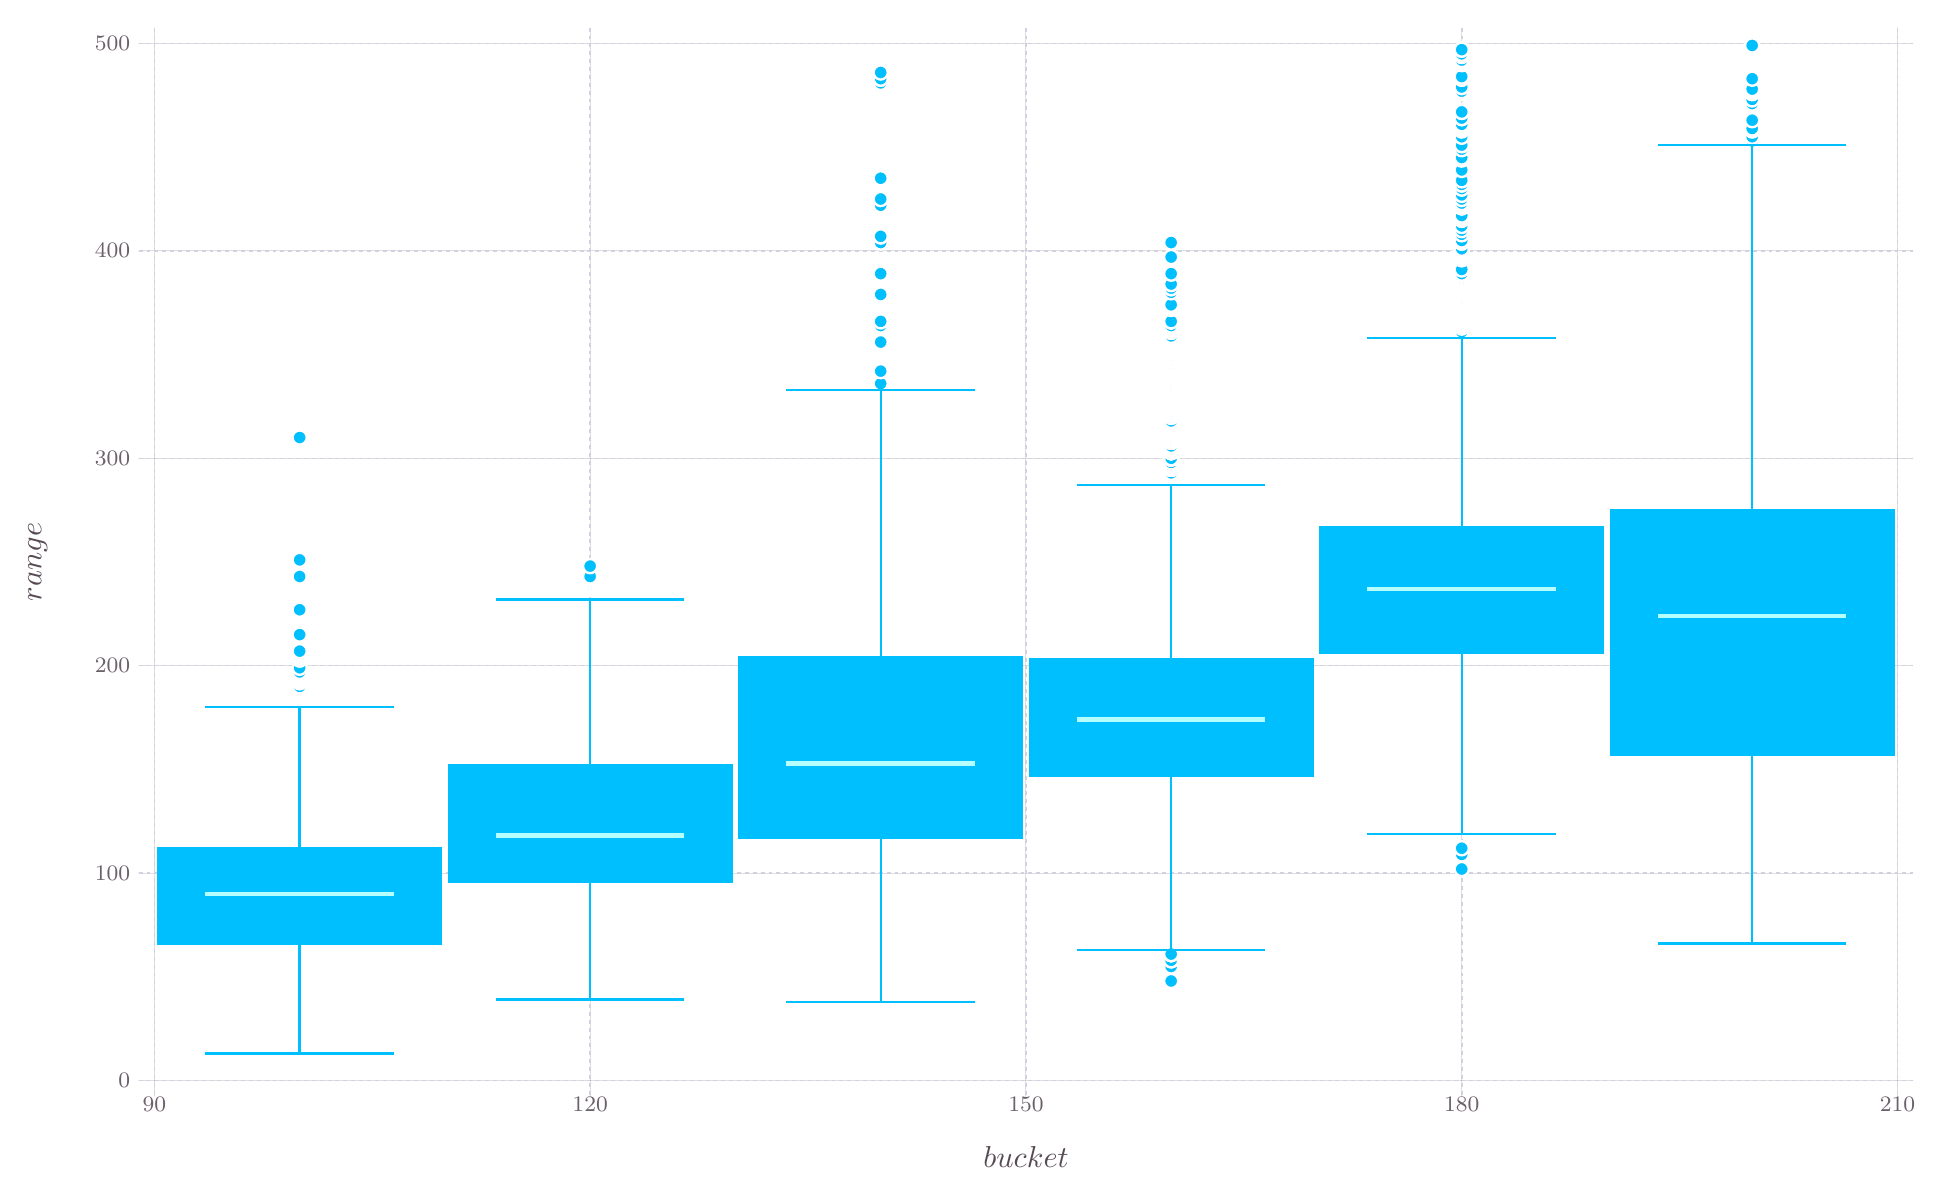
\begin{tikzpicture}[x=1mm,y=-1mm]
\definecolor{mycolor00BFFF}{rgb}{0,0.75,1}
\definecolor{mycolorD0D0E0}{rgb}{0.82,0.82,0.88}
\definecolor{mycolor000000}{rgb}{0,0,0}
\definecolor{mycolor564A55}{rgb}{0.34,0.29,0.33}
\definecolor{mycolor000000}{rgb}{0,0,0}
\definecolor{mycolorFFFFFF}{rgb}{1,1,1}
\definecolor{mycolorB5FFFF}{rgb}{0.71,1,1}
\definecolor{mycolor6C606B}{rgb}{0.42,0.38,0.42}
\begin{scope}
\begin{scope}
\draw (132.32,148.39) node [text=mycolor564A55,draw=mycolor000000,draw opacity=0,rotate around={-0: (0,1.81)},inner sep=0.0]{\fontsize{3.88mm}{4.66mm}\selectfont $\text{bucket}$};
\end{scope}
\begin{scope}
\draw (21.63,141.72) node [text=mycolor6C606B,rotate around={-0: (110.68,1.34)},inner sep=0.0]{\fontsize{2.82mm}{3.39mm}\selectfont $\text{90}$};
\draw (76.97,141.72) node [text=mycolor6C606B,rotate around={-0: (55.34,1.34)},inner sep=0.0]{\fontsize{2.82mm}{3.39mm}\selectfont $\text{120}$};
\draw (132.32,141.72) node [text=mycolor6C606B,rotate around={-0: (0,1.34)},inner sep=0.0]{\fontsize{2.82mm}{3.39mm}\selectfont $\text{150}$};
\draw (187.66,141.72) node [text=mycolor6C606B,rotate around={-0: (-55.34,1.34)},inner sep=0.0]{\fontsize{2.82mm}{3.39mm}\selectfont $\text{180}$};
\draw (243,141.72) node [text=mycolor6C606B,rotate around={-0: (-110.68,1.34)},inner sep=0.0]{\fontsize{2.82mm}{3.39mm}\selectfont $\text{210}$};
\end{scope}
\begin{scope}
\clip  (19.63,5) -- (245,5) -- (245,140.72) -- (19.63,140.72);
\begin{scope}
\clip  (19.63,5) -- (245,5) -- (245,140.72) -- (19.63,140.72);
\path [fill=mycolor000000,fill opacity=0,draw=mycolor000000,draw opacity=0] (19.63,5) rectangle +(225.37,135.72);
\end{scope}
\begin{scope}
[dash pattern=on 0.5mm off 0.5mm,line width=0.2mm]
\path [fill=mycolor000000,draw=mycolorD0D0E0]  (19.63,138.72) -- (245,138.72);
\path [fill=mycolor000000,draw=mycolorD0D0E0]  (19.63,112.37) -- (245,112.37);
\path [fill=mycolor000000,draw=mycolorD0D0E0]  (19.63,86.03) -- (245,86.03);
\path [fill=mycolor000000,draw=mycolorD0D0E0]  (19.63,59.69) -- (245,59.69);
\path [fill=mycolor000000,draw=mycolorD0D0E0]  (19.63,33.34) -- (245,33.34);
\path [fill=mycolor000000,draw=mycolorD0D0E0]  (19.63,7) -- (245,7);
\end{scope}
\begin{scope}
[dash pattern=on 0.5mm off 0.5mm,line width=0.2mm]
\path [fill=mycolor000000,draw=mycolorD0D0E0]  (21.63,5) -- (21.63,140.72);
\path [fill=mycolor000000,draw=mycolorD0D0E0]  (76.97,5) -- (76.97,140.72);
\path [fill=mycolor000000,draw=mycolorD0D0E0]  (132.32,5) -- (132.32,140.72);
\path [fill=mycolor000000,draw=mycolorD0D0E0]  (187.66,5) -- (187.66,140.72);
\path [fill=mycolor000000,draw=mycolorD0D0E0]  (243,5) -- (243,140.72);
\end{scope}
\begin{scope}
\begin{scope}
[line width=0.3mm]
\path [fill=mycolor00BFFF,draw=mycolorFFFFFF] (40.08,90.77) circle [radius=0.9];
\path [fill=mycolor00BFFF,draw=mycolorFFFFFF] (40.08,90.77) circle [radius=0.9];
\path [fill=mycolor00BFFF,draw=mycolorFFFFFF] (40.08,90.77) circle [radius=0.9];
\path [fill=mycolor00BFFF,draw=mycolorFFFFFF] (40.08,90.77) circle [radius=0.9];
\path [fill=mycolor00BFFF,draw=mycolorFFFFFF] (40.08,90.77) circle [radius=0.9];
\path [fill=mycolor00BFFF,draw=mycolorFFFFFF] (40.08,90.51) circle [radius=0.9];
\path [fill=mycolor00BFFF,draw=mycolorFFFFFF] (40.08,90.51) circle [radius=0.9];
\path [fill=mycolor00BFFF,draw=mycolorFFFFFF] (40.08,90.51) circle [radius=0.9];
\path [fill=mycolor00BFFF,draw=mycolorFFFFFF] (40.08,90.51) circle [radius=0.9];
\path [fill=mycolor00BFFF,draw=mycolorFFFFFF] (40.08,90.51) circle [radius=0.9];
\path [fill=mycolor00BFFF,draw=mycolorFFFFFF] (40.08,90.24) circle [radius=0.9];
\path [fill=mycolor00BFFF,draw=mycolorFFFFFF] (40.08,89.98) circle [radius=0.9];
\path [fill=mycolor00BFFF,draw=mycolorFFFFFF] (40.08,89.98) circle [radius=0.9];
\path [fill=mycolor00BFFF,draw=mycolorFFFFFF] (40.08,89.72) circle [radius=0.9];
\path [fill=mycolor00BFFF,draw=mycolorFFFFFF] (40.08,89.72) circle [radius=0.9];
\path [fill=mycolor00BFFF,draw=mycolorFFFFFF] (40.08,89.72) circle [radius=0.9];
\path [fill=mycolor00BFFF,draw=mycolorFFFFFF] (40.08,89.72) circle [radius=0.9];
\path [fill=mycolor00BFFF,draw=mycolorFFFFFF] (40.08,89.72) circle [radius=0.9];
\path [fill=mycolor00BFFF,draw=mycolorFFFFFF] (40.08,89.72) circle [radius=0.9];
\path [fill=mycolor00BFFF,draw=mycolorFFFFFF] (40.08,89.45) circle [radius=0.9];
\path [fill=mycolor00BFFF,draw=mycolorFFFFFF] (40.08,89.45) circle [radius=0.9];
\path [fill=mycolor00BFFF,draw=mycolorFFFFFF] (40.08,89.19) circle [radius=0.9];
\path [fill=mycolor00BFFF,draw=mycolorFFFFFF] (40.08,89.19) circle [radius=0.9];
\path [fill=mycolor00BFFF,draw=mycolorFFFFFF] (40.08,89.19) circle [radius=0.9];
\path [fill=mycolor00BFFF,draw=mycolorFFFFFF] (40.08,89.19) circle [radius=0.9];
\path [fill=mycolor00BFFF,draw=mycolorFFFFFF] (40.08,88.93) circle [radius=0.9];
\path [fill=mycolor00BFFF,draw=mycolorFFFFFF] (40.08,88.93) circle [radius=0.9];
\path [fill=mycolor00BFFF,draw=mycolorFFFFFF] (40.08,88.93) circle [radius=0.9];
\path [fill=mycolor00BFFF,draw=mycolorFFFFFF] (40.08,88.66) circle [radius=0.9];
\path [fill=mycolor00BFFF,draw=mycolorFFFFFF] (40.08,88.66) circle [radius=0.9];
\path [fill=mycolor00BFFF,draw=mycolorFFFFFF] (40.08,88.66) circle [radius=0.9];
\path [fill=mycolor00BFFF,draw=mycolorFFFFFF] (40.08,88.14) circle [radius=0.9];
\path [fill=mycolor00BFFF,draw=mycolorFFFFFF] (40.08,87.87) circle [radius=0.9];
\path [fill=mycolor00BFFF,draw=mycolorFFFFFF] (40.08,87.87) circle [radius=0.9];
\path [fill=mycolor00BFFF,draw=mycolorFFFFFF] (40.08,87.87) circle [radius=0.9];
\path [fill=mycolor00BFFF,draw=mycolorFFFFFF] (40.08,87.87) circle [radius=0.9];
\path [fill=mycolor00BFFF,draw=mycolorFFFFFF] (40.08,87.61) circle [radius=0.9];
\path [fill=mycolor00BFFF,draw=mycolorFFFFFF] (40.08,87.35) circle [radius=0.9];
\path [fill=mycolor00BFFF,draw=mycolorFFFFFF] (40.08,87.08) circle [radius=0.9];
\path [fill=mycolor00BFFF,draw=mycolorFFFFFF] (40.08,87.08) circle [radius=0.9];
\path [fill=mycolor00BFFF,draw=mycolorFFFFFF] (40.08,86.82) circle [radius=0.9];
\path [fill=mycolor00BFFF,draw=mycolorFFFFFF] (40.08,86.29) circle [radius=0.9];
\path [fill=mycolor00BFFF,draw=mycolorFFFFFF] (40.08,85.24) circle [radius=0.9];
\path [fill=mycolor00BFFF,draw=mycolorFFFFFF] (40.08,85.24) circle [radius=0.9];
\path [fill=mycolor00BFFF,draw=mycolorFFFFFF] (40.08,84.98) circle [radius=0.9];
\path [fill=mycolor00BFFF,draw=mycolorFFFFFF] (40.08,84.71) circle [radius=0.9];
\path [fill=mycolor00BFFF,draw=mycolorFFFFFF] (40.08,84.45) circle [radius=0.9];
\path [fill=mycolor00BFFF,draw=mycolorFFFFFF] (40.08,84.18) circle [radius=0.9];
\path [fill=mycolor00BFFF,draw=mycolorFFFFFF] (40.08,82.08) circle [radius=0.9];
\path [fill=mycolor00BFFF,draw=mycolorFFFFFF] (40.08,78.92) circle [radius=0.9];
\path [fill=mycolor00BFFF,draw=mycolorFFFFFF] (40.08,74.7) circle [radius=0.9];
\path [fill=mycolor00BFFF,draw=mycolorFFFFFF] (40.08,72.59) circle [radius=0.9];
\path [fill=mycolor00BFFF,draw=mycolorFFFFFF] (40.08,57.05) circle [radius=0.9];
\path [fill=mycolor00BFFF,draw=mycolorFFFFFF] (76.97,76.28) circle [radius=0.9];
\path [fill=mycolor00BFFF,draw=mycolorFFFFFF] (76.97,76.02) circle [radius=0.9];
\path [fill=mycolor00BFFF,draw=mycolorFFFFFF] (76.97,76.02) circle [radius=0.9];
\path [fill=mycolor00BFFF,draw=mycolorFFFFFF] (76.97,75.76) circle [radius=0.9];
\path [fill=mycolor00BFFF,draw=mycolorFFFFFF] (76.97,75.76) circle [radius=0.9];
\path [fill=mycolor00BFFF,draw=mycolorFFFFFF] (76.97,75.49) circle [radius=0.9];
\path [fill=mycolor00BFFF,draw=mycolorFFFFFF] (76.97,75.23) circle [radius=0.9];
\path [fill=mycolor00BFFF,draw=mycolorFFFFFF] (76.97,74.96) circle [radius=0.9];
\path [fill=mycolor00BFFF,draw=mycolorFFFFFF] (76.97,74.7) circle [radius=0.9];
\path [fill=mycolor00BFFF,draw=mycolorFFFFFF] (76.97,74.7) circle [radius=0.9];
\path [fill=mycolor00BFFF,draw=mycolorFFFFFF] (76.97,74.7) circle [radius=0.9];
\path [fill=mycolor00BFFF,draw=mycolorFFFFFF] (76.97,74.7) circle [radius=0.9];
\path [fill=mycolor00BFFF,draw=mycolorFFFFFF] (76.97,73.38) circle [radius=0.9];
\path [fill=mycolor00BFFF,draw=mycolorFFFFFF] (113.87,50.2) circle [radius=0.9];
\path [fill=mycolor00BFFF,draw=mycolorFFFFFF] (113.87,48.62) circle [radius=0.9];
\path [fill=mycolor00BFFF,draw=mycolorFFFFFF] (113.87,44.93) circle [radius=0.9];
\path [fill=mycolor00BFFF,draw=mycolorFFFFFF] (113.87,42.83) circle [radius=0.9];
\path [fill=mycolor00BFFF,draw=mycolorFFFFFF] (113.87,42.3) circle [radius=0.9];
\path [fill=mycolor00BFFF,draw=mycolorFFFFFF] (113.87,38.88) circle [radius=0.9];
\path [fill=mycolor00BFFF,draw=mycolorFFFFFF] (113.87,36.24) circle [radius=0.9];
\path [fill=mycolor00BFFF,draw=mycolorFFFFFF] (113.87,32.29) circle [radius=0.9];
\path [fill=mycolor00BFFF,draw=mycolorFFFFFF] (113.87,31.5) circle [radius=0.9];
\path [fill=mycolor00BFFF,draw=mycolorFFFFFF] (113.87,31.5) circle [radius=0.9];
\path [fill=mycolor00BFFF,draw=mycolorFFFFFF] (113.87,27.55) circle [radius=0.9];
\path [fill=mycolor00BFFF,draw=mycolorFFFFFF] (113.87,26.76) circle [radius=0.9];
\path [fill=mycolor00BFFF,draw=mycolorFFFFFF] (113.87,24.12) circle [radius=0.9];
\path [fill=mycolor00BFFF,draw=mycolorFFFFFF] (113.87,12.01) circle [radius=0.9];
\path [fill=mycolor00BFFF,draw=mycolorFFFFFF] (113.87,11.48) circle [radius=0.9];
\path [fill=mycolor00BFFF,draw=mycolorFFFFFF] (113.87,11.48) circle [radius=0.9];
\path [fill=mycolor00BFFF,draw=mycolorFFFFFF] (113.87,10.69) circle [radius=0.9];
\path [fill=mycolor00BFFF,draw=mycolorFFFFFF] (150.76,126.07) circle [radius=0.9];
\path [fill=mycolor00BFFF,draw=mycolorFFFFFF] (150.76,124.23) circle [radius=0.9];
\path [fill=mycolor00BFFF,draw=mycolorFFFFFF] (150.76,124.23) circle [radius=0.9];
\path [fill=mycolor00BFFF,draw=mycolorFFFFFF] (150.76,123.44) circle [radius=0.9];
\path [fill=mycolor00BFFF,draw=mycolorFFFFFF] (150.76,123.44) circle [radius=0.9];
\path [fill=mycolor00BFFF,draw=mycolorFFFFFF] (150.76,122.65) circle [radius=0.9];
\path [fill=mycolor00BFFF,draw=mycolorFFFFFF] (150.76,122.65) circle [radius=0.9];
\path [fill=mycolor00BFFF,draw=mycolorFFFFFF] (150.76,122.65) circle [radius=0.9];
\path [fill=mycolor00BFFF,draw=mycolorFFFFFF] (150.76,122.65) circle [radius=0.9];
\path [fill=mycolor00BFFF,draw=mycolorFFFFFF] (150.76,122.65) circle [radius=0.9];
\path [fill=mycolor00BFFF,draw=mycolorFFFFFF] (150.76,62.85) circle [radius=0.9];
\path [fill=mycolor00BFFF,draw=mycolorFFFFFF] (150.76,62.85) circle [radius=0.9];
\path [fill=mycolor00BFFF,draw=mycolorFFFFFF] (150.76,62.58) circle [radius=0.9];
\path [fill=mycolor00BFFF,draw=mycolorFFFFFF] (150.76,62.32) circle [radius=0.9];
\path [fill=mycolor00BFFF,draw=mycolorFFFFFF] (150.76,62.32) circle [radius=0.9];
\path [fill=mycolor00BFFF,draw=mycolorFFFFFF] (150.76,62.32) circle [radius=0.9];
\path [fill=mycolor00BFFF,draw=mycolorFFFFFF] (150.76,62.32) circle [radius=0.9];
\path [fill=mycolor00BFFF,draw=mycolorFFFFFF] (150.76,62.32) circle [radius=0.9];
\path [fill=mycolor00BFFF,draw=mycolorFFFFFF] (150.76,62.32) circle [radius=0.9];
\path [fill=mycolor00BFFF,draw=mycolorFFFFFF] (150.76,62.32) circle [radius=0.9];
\path [fill=mycolor00BFFF,draw=mycolorFFFFFF] (150.76,62.32) circle [radius=0.9];
\path [fill=mycolor00BFFF,draw=mycolorFFFFFF] (150.76,62.32) circle [radius=0.9];
\path [fill=mycolor00BFFF,draw=mycolorFFFFFF] (150.76,62.32) circle [radius=0.9];
\path [fill=mycolor00BFFF,draw=mycolorFFFFFF] (150.76,62.32) circle [radius=0.9];
\path [fill=mycolor00BFFF,draw=mycolorFFFFFF] (150.76,62.32) circle [radius=0.9];
\path [fill=mycolor00BFFF,draw=mycolorFFFFFF] (150.76,62.32) circle [radius=0.9];
\path [fill=mycolor00BFFF,draw=mycolorFFFFFF] (150.76,62.32) circle [radius=0.9];
\path [fill=mycolor00BFFF,draw=mycolorFFFFFF] (150.76,62.32) circle [radius=0.9];
\path [fill=mycolor00BFFF,draw=mycolorFFFFFF] (150.76,62.32) circle [radius=0.9];
\path [fill=mycolor00BFFF,draw=mycolorFFFFFF] (150.76,62.32) circle [radius=0.9];
\path [fill=mycolor00BFFF,draw=mycolorFFFFFF] (150.76,62.06) circle [radius=0.9];
\path [fill=mycolor00BFFF,draw=mycolorFFFFFF] (150.76,62.06) circle [radius=0.9];
\path [fill=mycolor00BFFF,draw=mycolorFFFFFF] (150.76,61.79) circle [radius=0.9];
\path [fill=mycolor00BFFF,draw=mycolorFFFFFF] (150.76,61.79) circle [radius=0.9];
\path [fill=mycolor00BFFF,draw=mycolorFFFFFF] (150.76,61.79) circle [radius=0.9];
\path [fill=mycolor00BFFF,draw=mycolorFFFFFF] (150.76,61.79) circle [radius=0.9];
\path [fill=mycolor00BFFF,draw=mycolorFFFFFF] (150.76,61.79) circle [radius=0.9];
\path [fill=mycolor00BFFF,draw=mycolorFFFFFF] (150.76,61.79) circle [radius=0.9];
\path [fill=mycolor00BFFF,draw=mycolorFFFFFF] (150.76,61.53) circle [radius=0.9];
\path [fill=mycolor00BFFF,draw=mycolorFFFFFF] (150.76,61) circle [radius=0.9];
\path [fill=mycolor00BFFF,draw=mycolorFFFFFF] (150.76,61) circle [radius=0.9];
\path [fill=mycolor00BFFF,draw=mycolorFFFFFF] (150.76,61) circle [radius=0.9];
\path [fill=mycolor00BFFF,draw=mycolorFFFFFF] (150.76,61) circle [radius=0.9];
\path [fill=mycolor00BFFF,draw=mycolorFFFFFF] (150.76,61) circle [radius=0.9];
\path [fill=mycolor00BFFF,draw=mycolorFFFFFF] (150.76,61) circle [radius=0.9];
\path [fill=mycolor00BFFF,draw=mycolorFFFFFF] (150.76,61) circle [radius=0.9];
\path [fill=mycolor00BFFF,draw=mycolorFFFFFF] (150.76,61) circle [radius=0.9];
\path [fill=mycolor00BFFF,draw=mycolorFFFFFF] (150.76,61) circle [radius=0.9];
\path [fill=mycolor00BFFF,draw=mycolorFFFFFF] (150.76,61) circle [radius=0.9];
\path [fill=mycolor00BFFF,draw=mycolorFFFFFF] (150.76,61) circle [radius=0.9];
\path [fill=mycolor00BFFF,draw=mycolorFFFFFF] (150.76,61) circle [radius=0.9];
\path [fill=mycolor00BFFF,draw=mycolorFFFFFF] (150.76,61) circle [radius=0.9];
\path [fill=mycolor00BFFF,draw=mycolorFFFFFF] (150.76,61) circle [radius=0.9];
\path [fill=mycolor00BFFF,draw=mycolorFFFFFF] (150.76,61) circle [radius=0.9];
\path [fill=mycolor00BFFF,draw=mycolorFFFFFF] (150.76,61) circle [radius=0.9];
\path [fill=mycolor00BFFF,draw=mycolorFFFFFF] (150.76,61) circle [radius=0.9];
\path [fill=mycolor00BFFF,draw=mycolorFFFFFF] (150.76,60.74) circle [radius=0.9];
\path [fill=mycolor00BFFF,draw=mycolorFFFFFF] (150.76,60.74) circle [radius=0.9];
\path [fill=mycolor00BFFF,draw=mycolorFFFFFF] (150.76,60.74) circle [radius=0.9];
\path [fill=mycolor00BFFF,draw=mycolorFFFFFF] (150.76,60.74) circle [radius=0.9];
\path [fill=mycolor00BFFF,draw=mycolorFFFFFF] (150.76,60.74) circle [radius=0.9];
\path [fill=mycolor00BFFF,draw=mycolorFFFFFF] (150.76,60.48) circle [radius=0.9];
\path [fill=mycolor00BFFF,draw=mycolorFFFFFF] (150.76,60.48) circle [radius=0.9];
\path [fill=mycolor00BFFF,draw=mycolorFFFFFF] (150.76,60.48) circle [radius=0.9];
\path [fill=mycolor00BFFF,draw=mycolorFFFFFF] (150.76,60.48) circle [radius=0.9];
\path [fill=mycolor00BFFF,draw=mycolorFFFFFF] (150.76,60.48) circle [radius=0.9];
\path [fill=mycolor00BFFF,draw=mycolorFFFFFF] (150.76,60.48) circle [radius=0.9];
\path [fill=mycolor00BFFF,draw=mycolorFFFFFF] (150.76,60.48) circle [radius=0.9];
\path [fill=mycolor00BFFF,draw=mycolorFFFFFF] (150.76,60.21) circle [radius=0.9];
\path [fill=mycolor00BFFF,draw=mycolorFFFFFF] (150.76,60.21) circle [radius=0.9];
\path [fill=mycolor00BFFF,draw=mycolorFFFFFF] (150.76,59.69) circle [radius=0.9];
\path [fill=mycolor00BFFF,draw=mycolorFFFFFF] (150.76,59.69) circle [radius=0.9];
\path [fill=mycolor00BFFF,draw=mycolorFFFFFF] (150.76,59.69) circle [radius=0.9];
\path [fill=mycolor00BFFF,draw=mycolorFFFFFF] (150.76,59.69) circle [radius=0.9];
\path [fill=mycolor00BFFF,draw=mycolorFFFFFF] (150.76,59.69) circle [radius=0.9];
\path [fill=mycolor00BFFF,draw=mycolorFFFFFF] (150.76,59.69) circle [radius=0.9];
\path [fill=mycolor00BFFF,draw=mycolorFFFFFF] (150.76,59.69) circle [radius=0.9];
\path [fill=mycolor00BFFF,draw=mycolorFFFFFF] (150.76,59.69) circle [radius=0.9];
\path [fill=mycolor00BFFF,draw=mycolorFFFFFF] (150.76,59.69) circle [radius=0.9];
\path [fill=mycolor00BFFF,draw=mycolorFFFFFF] (150.76,59.69) circle [radius=0.9];
\path [fill=mycolor00BFFF,draw=mycolorFFFFFF] (150.76,59.69) circle [radius=0.9];
\path [fill=mycolor00BFFF,draw=mycolorFFFFFF] (150.76,58.9) circle [radius=0.9];
\path [fill=mycolor00BFFF,draw=mycolorFFFFFF] (150.76,58.9) circle [radius=0.9];
\path [fill=mycolor00BFFF,draw=mycolorFFFFFF] (150.76,58.9) circle [radius=0.9];
\path [fill=mycolor00BFFF,draw=mycolorFFFFFF] (150.76,58.9) circle [radius=0.9];
\path [fill=mycolor00BFFF,draw=mycolorFFFFFF] (150.76,58.9) circle [radius=0.9];
\path [fill=mycolor00BFFF,draw=mycolorFFFFFF] (150.76,58.9) circle [radius=0.9];
\path [fill=mycolor00BFFF,draw=mycolorFFFFFF] (150.76,58.9) circle [radius=0.9];
\path [fill=mycolor00BFFF,draw=mycolorFFFFFF] (150.76,58.63) circle [radius=0.9];
\path [fill=mycolor00BFFF,draw=mycolorFFFFFF] (150.76,58.63) circle [radius=0.9];
\path [fill=mycolor00BFFF,draw=mycolorFFFFFF] (150.76,58.37) circle [radius=0.9];
\path [fill=mycolor00BFFF,draw=mycolorFFFFFF] (150.76,58.37) circle [radius=0.9];
\path [fill=mycolor00BFFF,draw=mycolorFFFFFF] (150.76,58.37) circle [radius=0.9];
\path [fill=mycolor00BFFF,draw=mycolorFFFFFF] (150.76,58.37) circle [radius=0.9];
\path [fill=mycolor00BFFF,draw=mycolorFFFFFF] (150.76,58.11) circle [radius=0.9];
\path [fill=mycolor00BFFF,draw=mycolorFFFFFF] (150.76,58.11) circle [radius=0.9];
\path [fill=mycolor00BFFF,draw=mycolorFFFFFF] (150.76,58.11) circle [radius=0.9];
\path [fill=mycolor00BFFF,draw=mycolorFFFFFF] (150.76,57.58) circle [radius=0.9];
\path [fill=mycolor00BFFF,draw=mycolorFFFFFF] (150.76,57.58) circle [radius=0.9];
\path [fill=mycolor00BFFF,draw=mycolorFFFFFF] (150.76,57.58) circle [radius=0.9];
\path [fill=mycolor00BFFF,draw=mycolorFFFFFF] (150.76,57.58) circle [radius=0.9];
\path [fill=mycolor00BFFF,draw=mycolorFFFFFF] (150.76,57.58) circle [radius=0.9];
\path [fill=mycolor00BFFF,draw=mycolorFFFFFF] (150.76,57.58) circle [radius=0.9];
\path [fill=mycolor00BFFF,draw=mycolorFFFFFF] (150.76,57.58) circle [radius=0.9];
\path [fill=mycolor00BFFF,draw=mycolorFFFFFF] (150.76,57.32) circle [radius=0.9];
\path [fill=mycolor00BFFF,draw=mycolorFFFFFF] (150.76,57.32) circle [radius=0.9];
\path [fill=mycolor00BFFF,draw=mycolorFFFFFF] (150.76,57.32) circle [radius=0.9];
\path [fill=mycolor00BFFF,draw=mycolorFFFFFF] (150.76,57.05) circle [radius=0.9];
\path [fill=mycolor00BFFF,draw=mycolorFFFFFF] (150.76,57.05) circle [radius=0.9];
\path [fill=mycolor00BFFF,draw=mycolorFFFFFF] (150.76,57.05) circle [radius=0.9];
\path [fill=mycolor00BFFF,draw=mycolorFFFFFF] (150.76,57.05) circle [radius=0.9];
\path [fill=mycolor00BFFF,draw=mycolorFFFFFF] (150.76,57.05) circle [radius=0.9];
\path [fill=mycolor00BFFF,draw=mycolorFFFFFF] (150.76,57.05) circle [radius=0.9];
\path [fill=mycolor00BFFF,draw=mycolorFFFFFF] (150.76,57.05) circle [radius=0.9];
\path [fill=mycolor00BFFF,draw=mycolorFFFFFF] (150.76,57.05) circle [radius=0.9];
\path [fill=mycolor00BFFF,draw=mycolorFFFFFF] (150.76,57.05) circle [radius=0.9];
\path [fill=mycolor00BFFF,draw=mycolorFFFFFF] (150.76,57.05) circle [radius=0.9];
\path [fill=mycolor00BFFF,draw=mycolorFFFFFF] (150.76,57.05) circle [radius=0.9];
\path [fill=mycolor00BFFF,draw=mycolorFFFFFF] (150.76,57.05) circle [radius=0.9];
\path [fill=mycolor00BFFF,draw=mycolorFFFFFF] (150.76,57.05) circle [radius=0.9];
\path [fill=mycolor00BFFF,draw=mycolorFFFFFF] (150.76,56.79) circle [radius=0.9];
\path [fill=mycolor00BFFF,draw=mycolorFFFFFF] (150.76,56.52) circle [radius=0.9];
\path [fill=mycolor00BFFF,draw=mycolorFFFFFF] (150.76,56.52) circle [radius=0.9];
\path [fill=mycolor00BFFF,draw=mycolorFFFFFF] (150.76,56.26) circle [radius=0.9];
\path [fill=mycolor00BFFF,draw=mycolorFFFFFF] (150.76,56.26) circle [radius=0.9];
\path [fill=mycolor00BFFF,draw=mycolorFFFFFF] (150.76,56.26) circle [radius=0.9];
\path [fill=mycolor00BFFF,draw=mycolorFFFFFF] (150.76,56) circle [radius=0.9];
\path [fill=mycolor00BFFF,draw=mycolorFFFFFF] (150.76,55.73) circle [radius=0.9];
\path [fill=mycolor00BFFF,draw=mycolorFFFFFF] (150.76,55.73) circle [radius=0.9];
\path [fill=mycolor00BFFF,draw=mycolorFFFFFF] (150.76,55.73) circle [radius=0.9];
\path [fill=mycolor00BFFF,draw=mycolorFFFFFF] (150.76,55.73) circle [radius=0.9];
\path [fill=mycolor00BFFF,draw=mycolorFFFFFF] (150.76,55.73) circle [radius=0.9];
\path [fill=mycolor00BFFF,draw=mycolorFFFFFF] (150.76,55.73) circle [radius=0.9];
\path [fill=mycolor00BFFF,draw=mycolorFFFFFF] (150.76,55.73) circle [radius=0.9];
\path [fill=mycolor00BFFF,draw=mycolorFFFFFF] (150.76,55.73) circle [radius=0.9];
\path [fill=mycolor00BFFF,draw=mycolorFFFFFF] (150.76,55.73) circle [radius=0.9];
\path [fill=mycolor00BFFF,draw=mycolorFFFFFF] (150.76,55.47) circle [radius=0.9];
\path [fill=mycolor00BFFF,draw=mycolorFFFFFF] (150.76,55.21) circle [radius=0.9];
\path [fill=mycolor00BFFF,draw=mycolorFFFFFF] (150.76,55.21) circle [radius=0.9];
\path [fill=mycolor00BFFF,draw=mycolorFFFFFF] (150.76,55.21) circle [radius=0.9];
\path [fill=mycolor00BFFF,draw=mycolorFFFFFF] (150.76,55.21) circle [radius=0.9];
\path [fill=mycolor00BFFF,draw=mycolorFFFFFF] (150.76,55.21) circle [radius=0.9];
\path [fill=mycolor00BFFF,draw=mycolorFFFFFF] (150.76,55.21) circle [radius=0.9];
\path [fill=mycolor00BFFF,draw=mycolorFFFFFF] (150.76,55.21) circle [radius=0.9];
\path [fill=mycolor00BFFF,draw=mycolorFFFFFF] (150.76,55.21) circle [radius=0.9];
\path [fill=mycolor00BFFF,draw=mycolorFFFFFF] (150.76,54.94) circle [radius=0.9];
\path [fill=mycolor00BFFF,draw=mycolorFFFFFF] (150.76,54.94) circle [radius=0.9];
\path [fill=mycolor00BFFF,draw=mycolorFFFFFF] (150.76,54.94) circle [radius=0.9];
\path [fill=mycolor00BFFF,draw=mycolorFFFFFF] (150.76,54.94) circle [radius=0.9];
\path [fill=mycolor00BFFF,draw=mycolorFFFFFF] (150.76,54.42) circle [radius=0.9];
\path [fill=mycolor00BFFF,draw=mycolorFFFFFF] (150.76,54.42) circle [radius=0.9];
\path [fill=mycolor00BFFF,draw=mycolorFFFFFF] (150.76,54.15) circle [radius=0.9];
\path [fill=mycolor00BFFF,draw=mycolorFFFFFF] (150.76,53.89) circle [radius=0.9];
\path [fill=mycolor00BFFF,draw=mycolorFFFFFF] (150.76,53.89) circle [radius=0.9];
\path [fill=mycolor00BFFF,draw=mycolorFFFFFF] (150.76,53.63) circle [radius=0.9];
\path [fill=mycolor00BFFF,draw=mycolorFFFFFF] (150.76,53.36) circle [radius=0.9];
\path [fill=mycolor00BFFF,draw=mycolorFFFFFF] (150.76,53.36) circle [radius=0.9];
\path [fill=mycolor00BFFF,draw=mycolorFFFFFF] (150.76,53.1) circle [radius=0.9];
\path [fill=mycolor00BFFF,draw=mycolorFFFFFF] (150.76,53.1) circle [radius=0.9];
\path [fill=mycolor00BFFF,draw=mycolorFFFFFF] (150.76,52.84) circle [radius=0.9];
\path [fill=mycolor00BFFF,draw=mycolorFFFFFF] (150.76,52.57) circle [radius=0.9];
\path [fill=mycolor00BFFF,draw=mycolorFFFFFF] (150.76,52.57) circle [radius=0.9];
\path [fill=mycolor00BFFF,draw=mycolorFFFFFF] (150.76,52.57) circle [radius=0.9];
\path [fill=mycolor00BFFF,draw=mycolorFFFFFF] (150.76,52.57) circle [radius=0.9];
\path [fill=mycolor00BFFF,draw=mycolorFFFFFF] (150.76,52.31) circle [radius=0.9];
\path [fill=mycolor00BFFF,draw=mycolorFFFFFF] (150.76,52.31) circle [radius=0.9];
\path [fill=mycolor00BFFF,draw=mycolorFFFFFF] (150.76,52.31) circle [radius=0.9];
\path [fill=mycolor00BFFF,draw=mycolorFFFFFF] (150.76,52.05) circle [radius=0.9];
\path [fill=mycolor00BFFF,draw=mycolorFFFFFF] (150.76,52.05) circle [radius=0.9];
\path [fill=mycolor00BFFF,draw=mycolorFFFFFF] (150.76,52.05) circle [radius=0.9];
\path [fill=mycolor00BFFF,draw=mycolorFFFFFF] (150.76,52.05) circle [radius=0.9];
\path [fill=mycolor00BFFF,draw=mycolorFFFFFF] (150.76,52.05) circle [radius=0.9];
\path [fill=mycolor00BFFF,draw=mycolorFFFFFF] (150.76,51.78) circle [radius=0.9];
\path [fill=mycolor00BFFF,draw=mycolorFFFFFF] (150.76,51.52) circle [radius=0.9];
\path [fill=mycolor00BFFF,draw=mycolorFFFFFF] (150.76,51.52) circle [radius=0.9];
\path [fill=mycolor00BFFF,draw=mycolorFFFFFF] (150.76,51.52) circle [radius=0.9];
\path [fill=mycolor00BFFF,draw=mycolorFFFFFF] (150.76,51.26) circle [radius=0.9];
\path [fill=mycolor00BFFF,draw=mycolorFFFFFF] (150.76,51.26) circle [radius=0.9];
\path [fill=mycolor00BFFF,draw=mycolorFFFFFF] (150.76,51.26) circle [radius=0.9];
\path [fill=mycolor00BFFF,draw=mycolorFFFFFF] (150.76,50.99) circle [radius=0.9];
\path [fill=mycolor00BFFF,draw=mycolorFFFFFF] (150.76,50.99) circle [radius=0.9];
\path [fill=mycolor00BFFF,draw=mycolorFFFFFF] (150.76,50.99) circle [radius=0.9];
\path [fill=mycolor00BFFF,draw=mycolorFFFFFF] (150.76,50.99) circle [radius=0.9];
\path [fill=mycolor00BFFF,draw=mycolorFFFFFF] (150.76,50.73) circle [radius=0.9];
\path [fill=mycolor00BFFF,draw=mycolorFFFFFF] (150.76,50.73) circle [radius=0.9];
\path [fill=mycolor00BFFF,draw=mycolorFFFFFF] (150.76,50.73) circle [radius=0.9];
\path [fill=mycolor00BFFF,draw=mycolorFFFFFF] (150.76,50.47) circle [radius=0.9];
\path [fill=mycolor00BFFF,draw=mycolorFFFFFF] (150.76,50.47) circle [radius=0.9];
\path [fill=mycolor00BFFF,draw=mycolorFFFFFF] (150.76,50.47) circle [radius=0.9];
\path [fill=mycolor00BFFF,draw=mycolorFFFFFF] (150.76,50.47) circle [radius=0.9];
\path [fill=mycolor00BFFF,draw=mycolorFFFFFF] (150.76,50.47) circle [radius=0.9];
\path [fill=mycolor00BFFF,draw=mycolorFFFFFF] (150.76,50.47) circle [radius=0.9];
\path [fill=mycolor00BFFF,draw=mycolorFFFFFF] (150.76,50.47) circle [radius=0.9];
\path [fill=mycolor00BFFF,draw=mycolorFFFFFF] (150.76,50.47) circle [radius=0.9];
\path [fill=mycolor00BFFF,draw=mycolorFFFFFF] (150.76,50.47) circle [radius=0.9];
\path [fill=mycolor00BFFF,draw=mycolorFFFFFF] (150.76,50.2) circle [radius=0.9];
\path [fill=mycolor00BFFF,draw=mycolorFFFFFF] (150.76,50.2) circle [radius=0.9];
\path [fill=mycolor00BFFF,draw=mycolorFFFFFF] (150.76,50.2) circle [radius=0.9];
\path [fill=mycolor00BFFF,draw=mycolorFFFFFF] (150.76,49.94) circle [radius=0.9];
\path [fill=mycolor00BFFF,draw=mycolorFFFFFF] (150.76,49.68) circle [radius=0.9];
\path [fill=mycolor00BFFF,draw=mycolorFFFFFF] (150.76,49.68) circle [radius=0.9];
\path [fill=mycolor00BFFF,draw=mycolorFFFFFF] (150.76,49.68) circle [radius=0.9];
\path [fill=mycolor00BFFF,draw=mycolorFFFFFF] (150.76,49.68) circle [radius=0.9];
\path [fill=mycolor00BFFF,draw=mycolorFFFFFF] (150.76,49.68) circle [radius=0.9];
\path [fill=mycolor00BFFF,draw=mycolorFFFFFF] (150.76,49.68) circle [radius=0.9];
\path [fill=mycolor00BFFF,draw=mycolorFFFFFF] (150.76,49.68) circle [radius=0.9];
\path [fill=mycolor00BFFF,draw=mycolorFFFFFF] (150.76,49.68) circle [radius=0.9];
\path [fill=mycolor00BFFF,draw=mycolorFFFFFF] (150.76,49.68) circle [radius=0.9];
\path [fill=mycolor00BFFF,draw=mycolorFFFFFF] (150.76,49.41) circle [radius=0.9];
\path [fill=mycolor00BFFF,draw=mycolorFFFFFF] (150.76,49.15) circle [radius=0.9];
\path [fill=mycolor00BFFF,draw=mycolorFFFFFF] (150.76,49.15) circle [radius=0.9];
\path [fill=mycolor00BFFF,draw=mycolorFFFFFF] (150.76,49.15) circle [radius=0.9];
\path [fill=mycolor00BFFF,draw=mycolorFFFFFF] (150.76,49.15) circle [radius=0.9];
\path [fill=mycolor00BFFF,draw=mycolorFFFFFF] (150.76,49.15) circle [radius=0.9];
\path [fill=mycolor00BFFF,draw=mycolorFFFFFF] (150.76,49.15) circle [radius=0.9];
\path [fill=mycolor00BFFF,draw=mycolorFFFFFF] (150.76,49.15) circle [radius=0.9];
\path [fill=mycolor00BFFF,draw=mycolorFFFFFF] (150.76,49.15) circle [radius=0.9];
\path [fill=mycolor00BFFF,draw=mycolorFFFFFF] (150.76,48.89) circle [radius=0.9];
\path [fill=mycolor00BFFF,draw=mycolorFFFFFF] (150.76,48.62) circle [radius=0.9];
\path [fill=mycolor00BFFF,draw=mycolorFFFFFF] (150.76,48.62) circle [radius=0.9];
\path [fill=mycolor00BFFF,draw=mycolorFFFFFF] (150.76,48.62) circle [radius=0.9];
\path [fill=mycolor00BFFF,draw=mycolorFFFFFF] (150.76,48.62) circle [radius=0.9];
\path [fill=mycolor00BFFF,draw=mycolorFFFFFF] (150.76,48.62) circle [radius=0.9];
\path [fill=mycolor00BFFF,draw=mycolorFFFFFF] (150.76,48.62) circle [radius=0.9];
\path [fill=mycolor00BFFF,draw=mycolorFFFFFF] (150.76,48.62) circle [radius=0.9];
\path [fill=mycolor00BFFF,draw=mycolorFFFFFF] (150.76,48.36) circle [radius=0.9];
\path [fill=mycolor00BFFF,draw=mycolorFFFFFF] (150.76,48.36) circle [radius=0.9];
\path [fill=mycolor00BFFF,draw=mycolorFFFFFF] (150.76,48.36) circle [radius=0.9];
\path [fill=mycolor00BFFF,draw=mycolorFFFFFF] (150.76,48.36) circle [radius=0.9];
\path [fill=mycolor00BFFF,draw=mycolorFFFFFF] (150.76,48.36) circle [radius=0.9];
\path [fill=mycolor00BFFF,draw=mycolorFFFFFF] (150.76,48.36) circle [radius=0.9];
\path [fill=mycolor00BFFF,draw=mycolorFFFFFF] (150.76,48.36) circle [radius=0.9];
\path [fill=mycolor00BFFF,draw=mycolorFFFFFF] (150.76,48.36) circle [radius=0.9];
\path [fill=mycolor00BFFF,draw=mycolorFFFFFF] (150.76,48.36) circle [radius=0.9];
\path [fill=mycolor00BFFF,draw=mycolorFFFFFF] (150.76,48.36) circle [radius=0.9];
\path [fill=mycolor00BFFF,draw=mycolorFFFFFF] (150.76,48.1) circle [radius=0.9];
\path [fill=mycolor00BFFF,draw=mycolorFFFFFF] (150.76,47.83) circle [radius=0.9];
\path [fill=mycolor00BFFF,draw=mycolorFFFFFF] (150.76,47.83) circle [radius=0.9];
\path [fill=mycolor00BFFF,draw=mycolorFFFFFF] (150.76,47.83) circle [radius=0.9];
\path [fill=mycolor00BFFF,draw=mycolorFFFFFF] (150.76,47.83) circle [radius=0.9];
\path [fill=mycolor00BFFF,draw=mycolorFFFFFF] (150.76,47.83) circle [radius=0.9];
\path [fill=mycolor00BFFF,draw=mycolorFFFFFF] (150.76,47.83) circle [radius=0.9];
\path [fill=mycolor00BFFF,draw=mycolorFFFFFF] (150.76,47.57) circle [radius=0.9];
\path [fill=mycolor00BFFF,draw=mycolorFFFFFF] (150.76,47.57) circle [radius=0.9];
\path [fill=mycolor00BFFF,draw=mycolorFFFFFF] (150.76,47.3) circle [radius=0.9];
\path [fill=mycolor00BFFF,draw=mycolorFFFFFF] (150.76,47.04) circle [radius=0.9];
\path [fill=mycolor00BFFF,draw=mycolorFFFFFF] (150.76,47.04) circle [radius=0.9];
\path [fill=mycolor00BFFF,draw=mycolorFFFFFF] (150.76,47.04) circle [radius=0.9];
\path [fill=mycolor00BFFF,draw=mycolorFFFFFF] (150.76,47.04) circle [radius=0.9];
\path [fill=mycolor00BFFF,draw=mycolorFFFFFF] (150.76,46.78) circle [radius=0.9];
\path [fill=mycolor00BFFF,draw=mycolorFFFFFF] (150.76,46.51) circle [radius=0.9];
\path [fill=mycolor00BFFF,draw=mycolorFFFFFF] (150.76,46.51) circle [radius=0.9];
\path [fill=mycolor00BFFF,draw=mycolorFFFFFF] (150.76,46.51) circle [radius=0.9];
\path [fill=mycolor00BFFF,draw=mycolorFFFFFF] (150.76,46.25) circle [radius=0.9];
\path [fill=mycolor00BFFF,draw=mycolorFFFFFF] (150.76,45.99) circle [radius=0.9];
\path [fill=mycolor00BFFF,draw=mycolorFFFFFF] (150.76,45.99) circle [radius=0.9];
\path [fill=mycolor00BFFF,draw=mycolorFFFFFF] (150.76,45.72) circle [radius=0.9];
\path [fill=mycolor00BFFF,draw=mycolorFFFFFF] (150.76,45.72) circle [radius=0.9];
\path [fill=mycolor00BFFF,draw=mycolorFFFFFF] (150.76,45.72) circle [radius=0.9];
\path [fill=mycolor00BFFF,draw=mycolorFFFFFF] (150.76,45.72) circle [radius=0.9];
\path [fill=mycolor00BFFF,draw=mycolorFFFFFF] (150.76,45.72) circle [radius=0.9];
\path [fill=mycolor00BFFF,draw=mycolorFFFFFF] (150.76,45.46) circle [radius=0.9];
\path [fill=mycolor00BFFF,draw=mycolorFFFFFF] (150.76,45.46) circle [radius=0.9];
\path [fill=mycolor00BFFF,draw=mycolorFFFFFF] (150.76,45.2) circle [radius=0.9];
\path [fill=mycolor00BFFF,draw=mycolorFFFFFF] (150.76,45.2) circle [radius=0.9];
\path [fill=mycolor00BFFF,draw=mycolorFFFFFF] (150.76,44.93) circle [radius=0.9];
\path [fill=mycolor00BFFF,draw=mycolorFFFFFF] (150.76,44.93) circle [radius=0.9];
\path [fill=mycolor00BFFF,draw=mycolorFFFFFF] (150.76,44.93) circle [radius=0.9];
\path [fill=mycolor00BFFF,draw=mycolorFFFFFF] (150.76,44.93) circle [radius=0.9];
\path [fill=mycolor00BFFF,draw=mycolorFFFFFF] (150.76,44.93) circle [radius=0.9];
\path [fill=mycolor00BFFF,draw=mycolorFFFFFF] (150.76,44.93) circle [radius=0.9];
\path [fill=mycolor00BFFF,draw=mycolorFFFFFF] (150.76,44.93) circle [radius=0.9];
\path [fill=mycolor00BFFF,draw=mycolorFFFFFF] (150.76,44.93) circle [radius=0.9];
\path [fill=mycolor00BFFF,draw=mycolorFFFFFF] (150.76,44.93) circle [radius=0.9];
\path [fill=mycolor00BFFF,draw=mycolorFFFFFF] (150.76,44.67) circle [radius=0.9];
\path [fill=mycolor00BFFF,draw=mycolorFFFFFF] (150.76,44.67) circle [radius=0.9];
\path [fill=mycolor00BFFF,draw=mycolorFFFFFF] (150.76,44.67) circle [radius=0.9];
\path [fill=mycolor00BFFF,draw=mycolorFFFFFF] (150.76,44.41) circle [radius=0.9];
\path [fill=mycolor00BFFF,draw=mycolorFFFFFF] (150.76,44.41) circle [radius=0.9];
\path [fill=mycolor00BFFF,draw=mycolorFFFFFF] (150.76,44.14) circle [radius=0.9];
\path [fill=mycolor00BFFF,draw=mycolorFFFFFF] (150.76,43.62) circle [radius=0.9];
\path [fill=mycolor00BFFF,draw=mycolorFFFFFF] (150.76,43.62) circle [radius=0.9];
\path [fill=mycolor00BFFF,draw=mycolorFFFFFF] (150.76,43.62) circle [radius=0.9];
\path [fill=mycolor00BFFF,draw=mycolorFFFFFF] (150.76,43.35) circle [radius=0.9];
\path [fill=mycolor00BFFF,draw=mycolorFFFFFF] (150.76,43.35) circle [radius=0.9];
\path [fill=mycolor00BFFF,draw=mycolorFFFFFF] (150.76,43.09) circle [radius=0.9];
\path [fill=mycolor00BFFF,draw=mycolorFFFFFF] (150.76,43.09) circle [radius=0.9];
\path [fill=mycolor00BFFF,draw=mycolorFFFFFF] (150.76,42.83) circle [radius=0.9];
\path [fill=mycolor00BFFF,draw=mycolorFFFFFF] (150.76,42.3) circle [radius=0.9];
\path [fill=mycolor00BFFF,draw=mycolorFFFFFF] (150.76,42.3) circle [radius=0.9];
\path [fill=mycolor00BFFF,draw=mycolorFFFFFF] (150.76,42.3) circle [radius=0.9];
\path [fill=mycolor00BFFF,draw=mycolorFFFFFF] (150.76,40.72) circle [radius=0.9];
\path [fill=mycolor00BFFF,draw=mycolorFFFFFF] (150.76,40.46) circle [radius=0.9];
\path [fill=mycolor00BFFF,draw=mycolorFFFFFF] (150.76,40.19) circle [radius=0.9];
\path [fill=mycolor00BFFF,draw=mycolorFFFFFF] (150.76,40.19) circle [radius=0.9];
\path [fill=mycolor00BFFF,draw=mycolorFFFFFF] (150.76,38.61) circle [radius=0.9];
\path [fill=mycolor00BFFF,draw=mycolorFFFFFF] (150.76,38.08) circle [radius=0.9];
\path [fill=mycolor00BFFF,draw=mycolorFFFFFF] (150.76,38.08) circle [radius=0.9];
\path [fill=mycolor00BFFF,draw=mycolorFFFFFF] (150.76,37.56) circle [radius=0.9];
\path [fill=mycolor00BFFF,draw=mycolorFFFFFF] (150.76,36.24) circle [radius=0.9];
\path [fill=mycolor00BFFF,draw=mycolorFFFFFF] (150.76,34.13) circle [radius=0.9];
\path [fill=mycolor00BFFF,draw=mycolorFFFFFF] (150.76,32.29) circle [radius=0.9];
\path [fill=mycolor00BFFF,draw=mycolorFFFFFF] (187.66,111.85) circle [radius=0.9];
\path [fill=mycolor00BFFF,draw=mycolorFFFFFF] (187.66,110) circle [radius=0.9];
\path [fill=mycolor00BFFF,draw=mycolorFFFFFF] (187.66,109.21) circle [radius=0.9];
\path [fill=mycolor00BFFF,draw=mycolorFFFFFF] (187.66,44.14) circle [radius=0.9];
\path [fill=mycolor00BFFF,draw=mycolorFFFFFF] (187.66,44.14) circle [radius=0.9];
\path [fill=mycolor00BFFF,draw=mycolorFFFFFF] (187.66,44.14) circle [radius=0.9];
\path [fill=mycolor00BFFF,draw=mycolorFFFFFF] (187.66,43.88) circle [radius=0.9];
\path [fill=mycolor00BFFF,draw=mycolorFFFFFF] (187.66,43.88) circle [radius=0.9];
\path [fill=mycolor00BFFF,draw=mycolorFFFFFF] (187.66,43.62) circle [radius=0.9];
\path [fill=mycolor00BFFF,draw=mycolorFFFFFF] (187.66,43.62) circle [radius=0.9];
\path [fill=mycolor00BFFF,draw=mycolorFFFFFF] (187.66,43.62) circle [radius=0.9];
\path [fill=mycolor00BFFF,draw=mycolorFFFFFF] (187.66,43.09) circle [radius=0.9];
\path [fill=mycolor00BFFF,draw=mycolorFFFFFF] (187.66,42.83) circle [radius=0.9];
\path [fill=mycolor00BFFF,draw=mycolorFFFFFF] (187.66,42.83) circle [radius=0.9];
\path [fill=mycolor00BFFF,draw=mycolorFFFFFF] (187.66,42.83) circle [radius=0.9];
\path [fill=mycolor00BFFF,draw=mycolorFFFFFF] (187.66,42.56) circle [radius=0.9];
\path [fill=mycolor00BFFF,draw=mycolorFFFFFF] (187.66,42.56) circle [radius=0.9];
\path [fill=mycolor00BFFF,draw=mycolorFFFFFF] (187.66,42.3) circle [radius=0.9];
\path [fill=mycolor00BFFF,draw=mycolorFFFFFF] (187.66,42.3) circle [radius=0.9];
\path [fill=mycolor00BFFF,draw=mycolorFFFFFF] (187.66,42.04) circle [radius=0.9];
\path [fill=mycolor00BFFF,draw=mycolorFFFFFF] (187.66,41.77) circle [radius=0.9];
\path [fill=mycolor00BFFF,draw=mycolorFFFFFF] (187.66,41.51) circle [radius=0.9];
\path [fill=mycolor00BFFF,draw=mycolorFFFFFF] (187.66,41.51) circle [radius=0.9];
\path [fill=mycolor00BFFF,draw=mycolorFFFFFF] (187.66,41.25) circle [radius=0.9];
\path [fill=mycolor00BFFF,draw=mycolorFFFFFF] (187.66,41.25) circle [radius=0.9];
\path [fill=mycolor00BFFF,draw=mycolorFFFFFF] (187.66,41.25) circle [radius=0.9];
\path [fill=mycolor00BFFF,draw=mycolorFFFFFF] (187.66,41.25) circle [radius=0.9];
\path [fill=mycolor00BFFF,draw=mycolorFFFFFF] (187.66,40.98) circle [radius=0.9];
\path [fill=mycolor00BFFF,draw=mycolorFFFFFF] (187.66,40.98) circle [radius=0.9];
\path [fill=mycolor00BFFF,draw=mycolorFFFFFF] (187.66,40.98) circle [radius=0.9];
\path [fill=mycolor00BFFF,draw=mycolorFFFFFF] (187.66,40.72) circle [radius=0.9];
\path [fill=mycolor00BFFF,draw=mycolorFFFFFF] (187.66,40.46) circle [radius=0.9];
\path [fill=mycolor00BFFF,draw=mycolorFFFFFF] (187.66,40.46) circle [radius=0.9];
\path [fill=mycolor00BFFF,draw=mycolorFFFFFF] (187.66,40.19) circle [radius=0.9];
\path [fill=mycolor00BFFF,draw=mycolorFFFFFF] (187.66,40.19) circle [radius=0.9];
\path [fill=mycolor00BFFF,draw=mycolorFFFFFF] (187.66,40.19) circle [radius=0.9];
\path [fill=mycolor00BFFF,draw=mycolorFFFFFF] (187.66,39.93) circle [radius=0.9];
\path [fill=mycolor00BFFF,draw=mycolorFFFFFF] (187.66,39.93) circle [radius=0.9];
\path [fill=mycolor00BFFF,draw=mycolorFFFFFF] (187.66,39.93) circle [radius=0.9];
\path [fill=mycolor00BFFF,draw=mycolorFFFFFF] (187.66,39.67) circle [radius=0.9];
\path [fill=mycolor00BFFF,draw=mycolorFFFFFF] (187.66,39.67) circle [radius=0.9];
\path [fill=mycolor00BFFF,draw=mycolorFFFFFF] (187.66,39.67) circle [radius=0.9];
\path [fill=mycolor00BFFF,draw=mycolorFFFFFF] (187.66,39.67) circle [radius=0.9];
\path [fill=mycolor00BFFF,draw=mycolorFFFFFF] (187.66,39.4) circle [radius=0.9];
\path [fill=mycolor00BFFF,draw=mycolorFFFFFF] (187.66,39.4) circle [radius=0.9];
\path [fill=mycolor00BFFF,draw=mycolorFFFFFF] (187.66,39.4) circle [radius=0.9];
\path [fill=mycolor00BFFF,draw=mycolorFFFFFF] (187.66,39.14) circle [radius=0.9];
\path [fill=mycolor00BFFF,draw=mycolorFFFFFF] (187.66,39.14) circle [radius=0.9];
\path [fill=mycolor00BFFF,draw=mycolorFFFFFF] (187.66,39.14) circle [radius=0.9];
\path [fill=mycolor00BFFF,draw=mycolorFFFFFF] (187.66,38.88) circle [radius=0.9];
\path [fill=mycolor00BFFF,draw=mycolorFFFFFF] (187.66,38.61) circle [radius=0.9];
\path [fill=mycolor00BFFF,draw=mycolorFFFFFF] (187.66,38.35) circle [radius=0.9];
\path [fill=mycolor00BFFF,draw=mycolorFFFFFF] (187.66,38.08) circle [radius=0.9];
\path [fill=mycolor00BFFF,draw=mycolorFFFFFF] (187.66,37.82) circle [radius=0.9];
\path [fill=mycolor00BFFF,draw=mycolorFFFFFF] (187.66,37.82) circle [radius=0.9];
\path [fill=mycolor00BFFF,draw=mycolorFFFFFF] (187.66,37.82) circle [radius=0.9];
\path [fill=mycolor00BFFF,draw=mycolorFFFFFF] (187.66,37.56) circle [radius=0.9];
\path [fill=mycolor00BFFF,draw=mycolorFFFFFF] (187.66,37.56) circle [radius=0.9];
\path [fill=mycolor00BFFF,draw=mycolorFFFFFF] (187.66,37.29) circle [radius=0.9];
\path [fill=mycolor00BFFF,draw=mycolorFFFFFF] (187.66,37.03) circle [radius=0.9];
\path [fill=mycolor00BFFF,draw=mycolorFFFFFF] (187.66,37.03) circle [radius=0.9];
\path [fill=mycolor00BFFF,draw=mycolorFFFFFF] (187.66,36.77) circle [radius=0.9];
\path [fill=mycolor00BFFF,draw=mycolorFFFFFF] (187.66,36.77) circle [radius=0.9];
\path [fill=mycolor00BFFF,draw=mycolorFFFFFF] (187.66,36.5) circle [radius=0.9];
\path [fill=mycolor00BFFF,draw=mycolorFFFFFF] (187.66,36.24) circle [radius=0.9];
\path [fill=mycolor00BFFF,draw=mycolorFFFFFF] (187.66,35.71) circle [radius=0.9];
\path [fill=mycolor00BFFF,draw=mycolorFFFFFF] (187.66,34.4) circle [radius=0.9];
\path [fill=mycolor00BFFF,draw=mycolorFFFFFF] (187.66,34.4) circle [radius=0.9];
\path [fill=mycolor00BFFF,draw=mycolorFFFFFF] (187.66,34.13) circle [radius=0.9];
\path [fill=mycolor00BFFF,draw=mycolorFFFFFF] (187.66,33.87) circle [radius=0.9];
\path [fill=mycolor00BFFF,draw=mycolorFFFFFF] (187.66,33.87) circle [radius=0.9];
\path [fill=mycolor00BFFF,draw=mycolorFFFFFF] (187.66,33.87) circle [radius=0.9];
\path [fill=mycolor00BFFF,draw=mycolorFFFFFF] (187.66,33.61) circle [radius=0.9];
\path [fill=mycolor00BFFF,draw=mycolorFFFFFF] (187.66,33.34) circle [radius=0.9];
\path [fill=mycolor00BFFF,draw=mycolorFFFFFF] (187.66,33.34) circle [radius=0.9];
\path [fill=mycolor00BFFF,draw=mycolorFFFFFF] (187.66,33.08) circle [radius=0.9];
\path [fill=mycolor00BFFF,draw=mycolorFFFFFF] (187.66,33.08) circle [radius=0.9];
\path [fill=mycolor00BFFF,draw=mycolorFFFFFF] (187.66,32.29) circle [radius=0.9];
\path [fill=mycolor00BFFF,draw=mycolorFFFFFF] (187.66,32.29) circle [radius=0.9];
\path [fill=mycolor00BFFF,draw=mycolorFFFFFF] (187.66,32.03) circle [radius=0.9];
\path [fill=mycolor00BFFF,draw=mycolorFFFFFF] (187.66,31.24) circle [radius=0.9];
\path [fill=mycolor00BFFF,draw=mycolorFFFFFF] (187.66,30.71) circle [radius=0.9];
\path [fill=mycolor00BFFF,draw=mycolorFFFFFF] (187.66,30.18) circle [radius=0.9];
\path [fill=mycolor00BFFF,draw=mycolorFFFFFF] (187.66,29.39) circle [radius=0.9];
\path [fill=mycolor00BFFF,draw=mycolorFFFFFF] (187.66,29.39) circle [radius=0.9];
\path [fill=mycolor00BFFF,draw=mycolorFFFFFF] (187.66,29.13) circle [radius=0.9];
\path [fill=mycolor00BFFF,draw=mycolorFFFFFF] (187.66,29.13) circle [radius=0.9];
\path [fill=mycolor00BFFF,draw=mycolorFFFFFF] (187.66,29.13) circle [radius=0.9];
\path [fill=mycolor00BFFF,draw=mycolorFFFFFF] (187.66,28.86) circle [radius=0.9];
\path [fill=mycolor00BFFF,draw=mycolorFFFFFF] (187.66,27.81) circle [radius=0.9];
\path [fill=mycolor00BFFF,draw=mycolorFFFFFF] (187.66,27.81) circle [radius=0.9];
\path [fill=mycolor00BFFF,draw=mycolorFFFFFF] (187.66,27.81) circle [radius=0.9];
\path [fill=mycolor00BFFF,draw=mycolorFFFFFF] (187.66,27.55) circle [radius=0.9];
\path [fill=mycolor00BFFF,draw=mycolorFFFFFF] (187.66,27.55) circle [radius=0.9];
\path [fill=mycolor00BFFF,draw=mycolorFFFFFF] (187.66,27.28) circle [radius=0.9];
\path [fill=mycolor00BFFF,draw=mycolorFFFFFF] (187.66,26.76) circle [radius=0.9];
\path [fill=mycolor00BFFF,draw=mycolorFFFFFF] (187.66,26.23) circle [radius=0.9];
\path [fill=mycolor00BFFF,draw=mycolorFFFFFF] (187.66,25.44) circle [radius=0.9];
\path [fill=mycolor00BFFF,draw=mycolorFFFFFF] (187.66,24.91) circle [radius=0.9];
\path [fill=mycolor00BFFF,draw=mycolorFFFFFF] (187.66,24.91) circle [radius=0.9];
\path [fill=mycolor00BFFF,draw=mycolorFFFFFF] (187.66,24.39) circle [radius=0.9];
\path [fill=mycolor00BFFF,draw=mycolorFFFFFF] (187.66,23.07) circle [radius=0.9];
\path [fill=mycolor00BFFF,draw=mycolorFFFFFF] (187.66,21.75) circle [radius=0.9];
\path [fill=mycolor00BFFF,draw=mycolorFFFFFF] (187.66,21.49) circle [radius=0.9];
\path [fill=mycolor00BFFF,draw=mycolorFFFFFF] (187.66,21.49) circle [radius=0.9];
\path [fill=mycolor00BFFF,draw=mycolorFFFFFF] (187.66,20.43) circle [radius=0.9];
\path [fill=mycolor00BFFF,draw=mycolorFFFFFF] (187.66,19.91) circle [radius=0.9];
\path [fill=mycolor00BFFF,draw=mycolorFFFFFF] (187.66,19.91) circle [radius=0.9];
\path [fill=mycolor00BFFF,draw=mycolorFFFFFF] (187.66,18.85) circle [radius=0.9];
\path [fill=mycolor00BFFF,draw=mycolorFFFFFF] (187.66,18.06) circle [radius=0.9];
\path [fill=mycolor00BFFF,draw=mycolorFFFFFF] (187.66,17.8) circle [radius=0.9];
\path [fill=mycolor00BFFF,draw=mycolorFFFFFF] (187.66,17.8) circle [radius=0.9];
\path [fill=mycolor00BFFF,draw=mycolorFFFFFF] (187.66,17.54) circle [radius=0.9];
\path [fill=mycolor00BFFF,draw=mycolorFFFFFF] (187.66,17.27) circle [radius=0.9];
\path [fill=mycolor00BFFF,draw=mycolorFFFFFF] (187.66,16.48) circle [radius=0.9];
\path [fill=mycolor00BFFF,draw=mycolorFFFFFF] (187.66,16.48) circle [radius=0.9];
\path [fill=mycolor00BFFF,draw=mycolorFFFFFF] (187.66,15.69) circle [radius=0.9];
\path [fill=mycolor00BFFF,draw=mycolorFFFFFF] (187.66,15.69) circle [radius=0.9];
\path [fill=mycolor00BFFF,draw=mycolorFFFFFF] (187.66,13.32) circle [radius=0.9];
\path [fill=mycolor00BFFF,draw=mycolorFFFFFF] (187.66,13.06) circle [radius=0.9];
\path [fill=mycolor00BFFF,draw=mycolorFFFFFF] (187.66,13.06) circle [radius=0.9];
\path [fill=mycolor00BFFF,draw=mycolorFFFFFF] (187.66,12.53) circle [radius=0.9];
\path [fill=mycolor00BFFF,draw=mycolorFFFFFF] (187.66,12.53) circle [radius=0.9];
\path [fill=mycolor00BFFF,draw=mycolorFFFFFF] (187.66,11.48) circle [radius=0.9];
\path [fill=mycolor00BFFF,draw=mycolorFFFFFF] (187.66,11.48) circle [radius=0.9];
\path [fill=mycolor00BFFF,draw=mycolorFFFFFF] (187.66,11.21) circle [radius=0.9];
\path [fill=mycolor00BFFF,draw=mycolorFFFFFF] (187.66,9.63) circle [radius=0.9];
\path [fill=mycolor00BFFF,draw=mycolorFFFFFF] (187.66,9.37) circle [radius=0.9];
\path [fill=mycolor00BFFF,draw=mycolorFFFFFF] (187.66,9.11) circle [radius=0.9];
\path [fill=mycolor00BFFF,draw=mycolorFFFFFF] (187.66,8.58) circle [radius=0.9];
\path [fill=mycolor00BFFF,draw=mycolorFFFFFF] (187.66,8.58) circle [radius=0.9];
\path [fill=mycolor00BFFF,draw=mycolorFFFFFF] (187.66,8.32) circle [radius=0.9];
\path [fill=mycolor00BFFF,draw=mycolorFFFFFF] (187.66,7.79) circle [radius=0.9];
\path [fill=mycolor00BFFF,draw=mycolorFFFFFF] (187.66,7.79) circle [radius=0.9];
\path [fill=mycolor00BFFF,draw=mycolorFFFFFF] (224.55,19.38) circle [radius=0.9];
\path [fill=mycolor00BFFF,draw=mycolorFFFFFF] (224.55,18.85) circle [radius=0.9];
\path [fill=mycolor00BFFF,draw=mycolorFFFFFF] (224.55,18.85) circle [radius=0.9];
\path [fill=mycolor00BFFF,draw=mycolorFFFFFF] (224.55,18.06) circle [radius=0.9];
\path [fill=mycolor00BFFF,draw=mycolorFFFFFF] (224.55,17.8) circle [radius=0.9];
\path [fill=mycolor00BFFF,draw=mycolorFFFFFF] (224.55,16.75) circle [radius=0.9];
\path [fill=mycolor00BFFF,draw=mycolorFFFFFF] (224.55,14.64) circle [radius=0.9];
\path [fill=mycolor00BFFF,draw=mycolorFFFFFF] (224.55,14.11) circle [radius=0.9];
\path [fill=mycolor00BFFF,draw=mycolorFFFFFF] (224.55,13.32) circle [radius=0.9];
\path [fill=mycolor00BFFF,draw=mycolorFFFFFF] (224.55,13.06) circle [radius=0.9];
\path [fill=mycolor00BFFF,draw=mycolorFFFFFF] (224.55,12.8) circle [radius=0.9];
\path [fill=mycolor00BFFF,draw=mycolorFFFFFF] (224.55,11.48) circle [radius=0.9];
\path [fill=mycolor00BFFF,draw=mycolorFFFFFF] (224.55,7.26) circle [radius=0.9];
\path [fill=mycolor00BFFF,draw=mycolorFFFFFF] (224.55,7.26) circle [radius=0.9];
\path [fill=mycolor00BFFF,draw=mycolor00BFFF] (22.13,109.21) rectangle +(35.89,12.12);
\path [fill=mycolor00BFFF,draw=mycolor00BFFF] (59.03,98.67) rectangle +(35.89,14.75);
\path [fill=mycolor00BFFF,draw=mycolor00BFFF] (95.92,84.98) rectangle +(35.89,22.92);
\path [fill=mycolor00BFFF,draw=mycolor00BFFF] (132.82,85.24) rectangle +(35.89,14.75);
\path [fill=mycolor00BFFF,draw=mycolor00BFFF] (169.71,68.38) rectangle +(35.89,16.07);
\path [fill=mycolor00BFFF,draw=mycolor00BFFF] (206.61,66.27) rectangle +(35.89,31.08);
\path [fill=mycolor00BFFF,draw=mycolor00BFFF]  (28.11,91.3) -- (52.04,91.3);
\path [fill=mycolor00BFFF,draw=mycolor00BFFF]  (65.01,77.6) -- (88.94,77.6);
\path [fill=mycolor00BFFF,draw=mycolor00BFFF]  (101.9,50.99) -- (125.83,50.99);
\path [fill=mycolor00BFFF,draw=mycolor00BFFF]  (138.8,63.11) -- (162.73,63.11);
\path [fill=mycolor00BFFF,draw=mycolor00BFFF]  (175.69,44.41) -- (199.62,44.41);
\path [fill=mycolor00BFFF,draw=mycolor00BFFF]  (212.59,19.91) -- (236.52,19.91);
\path [fill=mycolor00BFFF,draw=mycolor00BFFF]  (28.11,135.29) -- (52.04,135.29);
\path [fill=mycolor00BFFF,draw=mycolor00BFFF]  (65.01,128.44) -- (88.94,128.44);
\path [fill=mycolor00BFFF,draw=mycolor00BFFF]  (101.9,128.7) -- (125.83,128.7);
\path [fill=mycolor00BFFF,draw=mycolor00BFFF]  (138.8,122.12) -- (162.73,122.12);
\path [fill=mycolor00BFFF,draw=mycolor00BFFF]  (175.69,107.37) -- (199.62,107.37);
\path [fill=mycolor00BFFF,draw=mycolor00BFFF]  (212.59,121.33) -- (236.52,121.33);
\path [fill=mycolor00BFFF,draw=mycolor00BFFF]  (40.08,109.21) -- (40.08,91.3);
\path [fill=mycolor00BFFF,draw=mycolor00BFFF]  (76.97,98.67) -- (76.97,77.6);
\path [fill=mycolor00BFFF,draw=mycolor00BFFF]  (113.87,84.98) -- (113.87,50.99);
\path [fill=mycolor00BFFF,draw=mycolor00BFFF]  (150.76,85.24) -- (150.76,63.11);
\path [fill=mycolor00BFFF,draw=mycolor00BFFF]  (187.66,68.38) -- (187.66,44.41);
\path [fill=mycolor00BFFF,draw=mycolor00BFFF]  (224.55,66.27) -- (224.55,19.91);
\path [fill=mycolor00BFFF,draw=mycolor00BFFF]  (40.08,121.33) -- (40.08,135.29);
\path [fill=mycolor00BFFF,draw=mycolor00BFFF]  (76.97,113.43) -- (76.97,128.44);
\path [fill=mycolor00BFFF,draw=mycolor00BFFF]  (113.87,107.89) -- (113.87,128.7);
\path [fill=mycolor00BFFF,draw=mycolor00BFFF]  (150.76,99.99) -- (150.76,122.12);
\path [fill=mycolor00BFFF,draw=mycolor00BFFF]  (187.66,84.45) -- (187.66,107.37);
\path [fill=mycolor00BFFF,draw=mycolor00BFFF]  (224.55,97.36) -- (224.55,121.33);
\begin{scope}
[line width=0.6mm]
\path [fill=mycolor00BFFF,draw=mycolorB5FFFF]  (28.11,115.01) -- (52.04,115.01);
\path [fill=mycolor00BFFF,draw=mycolorB5FFFF]  (65.01,107.63) -- (88.94,107.63);
\path [fill=mycolor00BFFF,draw=mycolorB5FFFF]  (101.9,98.41) -- (125.83,98.41);
\path [fill=mycolor00BFFF,draw=mycolorB5FFFF]  (138.8,92.88) -- (162.73,92.88);
\path [fill=mycolor00BFFF,draw=mycolorB5FFFF]  (175.69,76.28) -- (199.62,76.28);
\path [fill=mycolor00BFFF,draw=mycolorB5FFFF]  (212.59,79.71) -- (236.52,79.71);
\end{scope}
\end{scope}
\end{scope}
\end{scope}
\begin{scope}
\draw (18.63,138.72) node [text=mycolor6C606B,rotate around={-0: (-2.51,-65.86)},left,inner sep=0.0]{\fontsize{2.82mm}{3.39mm}\selectfont $\text{0}$};
\draw (18.63,112.37) node [text=mycolor6C606B,rotate around={-0: (-2.51,-39.51)},left,inner sep=0.0]{\fontsize{2.82mm}{3.39mm}\selectfont $\text{100}$};
\draw (18.63,86.03) node [text=mycolor6C606B,rotate around={-0: (-2.51,-13.17)},left,inner sep=0.0]{\fontsize{2.82mm}{3.39mm}\selectfont $\text{200}$};
\draw (18.63,59.69) node [text=mycolor6C606B,rotate around={-0: (-2.51,13.17)},left,inner sep=0.0]{\fontsize{2.82mm}{3.39mm}\selectfont $\text{300}$};
\draw (18.63,33.34) node [text=mycolor6C606B,rotate around={-0: (-2.51,39.51)},left,inner sep=0.0]{\fontsize{2.82mm}{3.39mm}\selectfont $\text{400}$};
\draw (18.63,7) node [text=mycolor6C606B,rotate around={-0: (-2.51,65.86)},left,inner sep=0.0]{\fontsize{2.82mm}{3.39mm}\selectfont $\text{500}$};
\end{scope}
\begin{scope}
\draw (8.81,70.86) node [text=mycolor564A55,draw=mycolor000000,draw opacity=0,rotate around={90: (0,2)},inner sep=0.0]{\fontsize{3.88mm}{4.66mm}\selectfont $\text{range}$};
\end{scope}
\end{scope}
\end{tikzpicture}

%		\caption{Range values with \SI{1}{\centi\metre} resolution each bar represents all the values in the range, with bucket size of \SI{20}{\centi\metre}}
%		\label{buckets}
%	\end{figure}
%\end{landscape}
%\todo{caption for buckets (wording)}


\subsection{Influence of DQF on Range Values}
One value the ranging api provides is the DQF\footnote{Data Quality Factor}-value.
It is reasonable to expect a huge amount of scatter for lower DQF values.
As can be seen in \autoref{1m_scatterplot} this expectation is not met.

%For the values measured with \SI{1}{\metre} real distance we can see that the values measered with lower quality do not have the same mean value as those with higher quality.
%Also values measured with lower quality are closer to each other than those with higher signal quality.
%As long as we only look at the values taken at \SI{1}{\metre} real distance it seams like we could be able to improve the range estimate by including the dqf value into the computation of the distance.
%To do that this behaviour would need to be stable accross different distances, i.e. no matter if the measurement is taken at \SI{1}{\metre} or \SI{3}{\metre} distance the when the dqf is low the measured range is lower and if dqf is high the measured range is higher.
\begin{figure}[h]
	\centering
	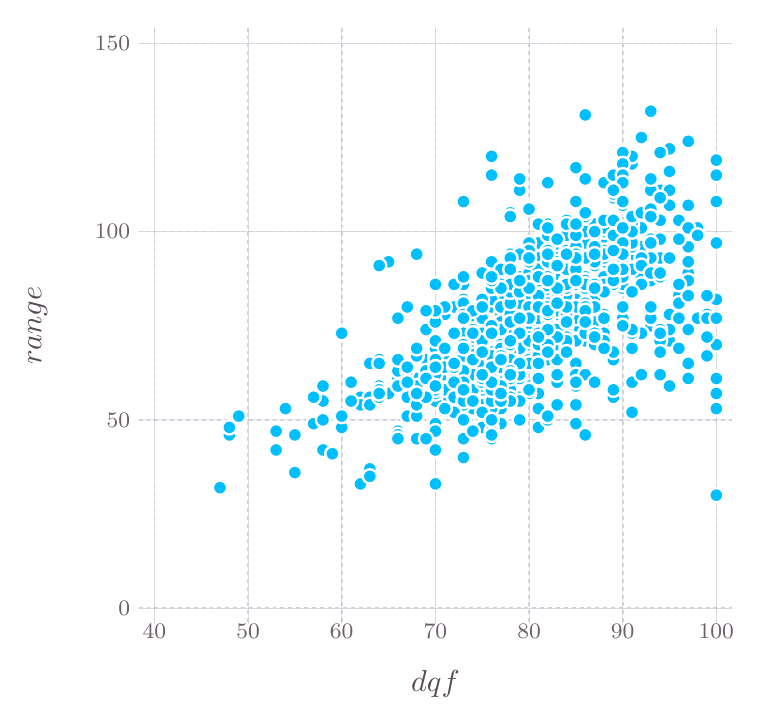
\begin{tikzpicture}[x=1mm,y=-1mm]
\definecolor{mycolor00BFFF}{rgb}{0,0.75,1}
\definecolor{mycolor564A55}{rgb}{0.34,0.29,0.33}
\definecolor{mycolor000000}{rgb}{0,0,0}
\definecolor{mycolor6C606B}{rgb}{0.42,0.38,0.42}
\definecolor{mycolorD0D0E0}{rgb}{0.82,0.82,0.88}
\definecolor{mycolorFFFFFF}{rgb}{1,1,1}
\definecolor{mycolor000000}{rgb}{0,0,0}
\begin{scope}
\begin{scope}
\draw (57.32,88.39) node [text=mycolor564A55,draw=mycolor000000,draw opacity=0,rotate around={-0: (0,1.81)},inner sep=0.0]{\fontsize{3.88mm}{4.66mm}\selectfont $\text{dqf}$};
\end{scope}
\begin{scope}
\draw (21.63,81.72) node [text=mycolor6C606B,rotate around={-0: (35.68,1.34)},inner sep=0.0]{\fontsize{2.82mm}{3.39mm}\selectfont $\text{40}$};
\draw (33.53,81.72) node [text=mycolor6C606B,rotate around={-0: (23.79,1.34)},inner sep=0.0]{\fontsize{2.82mm}{3.39mm}\selectfont $\text{50}$};
\draw (45.42,81.72) node [text=mycolor6C606B,rotate around={-0: (11.89,1.34)},inner sep=0.0]{\fontsize{2.82mm}{3.39mm}\selectfont $\text{60}$};
\draw (57.32,81.72) node [text=mycolor6C606B,rotate around={-0: (-0,1.34)},inner sep=0.0]{\fontsize{2.82mm}{3.39mm}\selectfont $\text{70}$};
\draw (69.21,81.72) node [text=mycolor6C606B,rotate around={-0: (-11.89,1.34)},inner sep=0.0]{\fontsize{2.82mm}{3.39mm}\selectfont $\text{80}$};
\draw (81.11,81.72) node [text=mycolor6C606B,rotate around={-0: (-23.79,1.34)},inner sep=0.0]{\fontsize{2.82mm}{3.39mm}\selectfont $\text{90}$};
\draw (93,81.72) node [text=mycolor6C606B,rotate around={-0: (-35.68,1.34)},inner sep=0.0]{\fontsize{2.82mm}{3.39mm}\selectfont $\text{100}$};
\end{scope}
\begin{scope}
\clip  (19.63,5) -- (95,5) -- (95,80.72) -- (19.63,80.72);
\begin{scope}
\clip  (19.63,5) -- (95,5) -- (95,80.72) -- (19.63,80.72);
\path [fill=mycolor000000,fill opacity=0,draw=mycolor000000,draw opacity=0] (19.63,5) rectangle +(75.37,75.72);
\end{scope}
\begin{scope}
[dash pattern=on 0.5mm off 0.5mm,line width=0.2mm]
\path [fill=mycolor000000,draw=mycolorD0D0E0]  (19.63,78.71) -- (95,78.71);
\path [fill=mycolor000000,draw=mycolorD0D0E0]  (19.63,54.81) -- (95,54.81);
\path [fill=mycolor000000,draw=mycolorD0D0E0]  (19.63,30.9) -- (95,30.9);
\path [fill=mycolor000000,draw=mycolorD0D0E0]  (19.63,7) -- (95,7);
\end{scope}
\begin{scope}
[dash pattern=on 0.5mm off 0.5mm,line width=0.2mm]
\path [fill=mycolor000000,draw=mycolorD0D0E0]  (21.63,5) -- (21.63,80.72);
\path [fill=mycolor000000,draw=mycolorD0D0E0]  (33.53,5) -- (33.53,80.72);
\path [fill=mycolor000000,draw=mycolorD0D0E0]  (45.42,5) -- (45.42,80.72);
\path [fill=mycolor000000,draw=mycolorD0D0E0]  (57.32,5) -- (57.32,80.72);
\path [fill=mycolor000000,draw=mycolorD0D0E0]  (69.21,5) -- (69.21,80.72);
\path [fill=mycolor000000,draw=mycolorD0D0E0]  (81.11,5) -- (81.11,80.72);
\path [fill=mycolor000000,draw=mycolorD0D0E0]  (93,5) -- (93,80.72);
\end{scope}
\begin{scope}
\begin{scope}
\begin{scope}
[line width=0.3mm]
\path [fill=mycolor00BFFF,draw=mycolorFFFFFF] (66.83,28.51) circle [radius=0.9];
\path [fill=mycolor00BFFF,draw=mycolorFFFFFF] (84.67,42.86) circle [radius=0.9];
\path [fill=mycolor00BFFF,draw=mycolorFFFFFF] (50.18,47.16) circle [radius=0.9];
\path [fill=mycolor00BFFF,draw=mycolorFFFFFF] (88.24,39.03) circle [radius=0.9];
\path [fill=mycolor00BFFF,draw=mycolorFFFFFF] (87.05,43.34) circle [radius=0.9];
\path [fill=mycolor00BFFF,draw=mycolorFFFFFF] (57.32,56.24) circle [radius=0.9];
\path [fill=mycolor00BFFF,draw=mycolorFFFFFF] (71.59,40.95) circle [radius=0.9];
\path [fill=mycolor00BFFF,draw=mycolorFFFFFF] (78.73,38.55) circle [radius=0.9];
\path [fill=mycolor00BFFF,draw=mycolorFFFFFF] (72.78,41.42) circle [radius=0.9];
\path [fill=mycolor00BFFF,draw=mycolorFFFFFF] (69.21,43.81) circle [radius=0.9];
\path [fill=mycolor00BFFF,draw=mycolorFFFFFF] (73.97,39.03) circle [radius=0.9];
\path [fill=mycolor00BFFF,draw=mycolorFFFFFF] (77.54,41.9) circle [radius=0.9];
\path [fill=mycolor00BFFF,draw=mycolorFFFFFF] (52.56,49.07) circle [radius=0.9];
\path [fill=mycolor00BFFF,draw=mycolorFFFFFF] (76.35,36.64) circle [radius=0.9];
\path [fill=mycolor00BFFF,draw=mycolorFFFFFF] (63.26,51.46) circle [radius=0.9];
\path [fill=mycolor00BFFF,draw=mycolorFFFFFF] (62.07,46.68) circle [radius=0.9];
\path [fill=mycolor00BFFF,draw=mycolorFFFFFF] (70.4,45.25) circle [radius=0.9];
\path [fill=mycolor00BFFF,draw=mycolorFFFFFF] (60.88,50.99) circle [radius=0.9];
\path [fill=mycolor00BFFF,draw=mycolorFFFFFF] (66.83,47.16) circle [radius=0.9];
\path [fill=mycolor00BFFF,draw=mycolorFFFFFF] (76.35,44.77) circle [radius=0.9];
\path [fill=mycolor00BFFF,draw=mycolorFFFFFF] (87.05,44.77) circle [radius=0.9];
\path [fill=mycolor00BFFF,draw=mycolorFFFFFF] (58.51,52.42) circle [radius=0.9];
\path [fill=mycolor00BFFF,draw=mycolorFFFFFF] (63.26,50.51) circle [radius=0.9];
\path [fill=mycolor00BFFF,draw=mycolorFFFFFF] (87.05,43.34) circle [radius=0.9];
\path [fill=mycolor00BFFF,draw=mycolorFFFFFF] (66.83,46.68) circle [radius=0.9];
\path [fill=mycolor00BFFF,draw=mycolorFFFFFF] (93,32.34) circle [radius=0.9];
\path [fill=mycolor00BFFF,draw=mycolorFFFFFF] (57.32,55.29) circle [radius=0.9];
\path [fill=mycolor00BFFF,draw=mycolorFFFFFF] (64.45,57.2) circle [radius=0.9];
\path [fill=mycolor00BFFF,draw=mycolorFFFFFF] (78.73,42.38) circle [radius=0.9];
\path [fill=mycolor00BFFF,draw=mycolorFFFFFF] (87.05,27.56) circle [radius=0.9];
\path [fill=mycolor00BFFF,draw=mycolorFFFFFF] (82.29,22.3) circle [radius=0.9];
\path [fill=mycolor00BFFF,draw=mycolorFFFFFF] (82.29,34.25) circle [radius=0.9];
\path [fill=mycolor00BFFF,draw=mycolorFFFFFF] (71.59,39.03) circle [radius=0.9];
\path [fill=mycolor00BFFF,draw=mycolorFFFFFF] (64.45,38.08) circle [radius=0.9];
\path [fill=mycolor00BFFF,draw=mycolorFFFFFF] (78.73,31.86) circle [radius=0.9];
\path [fill=mycolor00BFFF,draw=mycolorFFFFFF] (60.88,49.55) circle [radius=0.9];
\path [fill=mycolor00BFFF,draw=mycolorFFFFFF] (71.59,35.69) circle [radius=0.9];
\path [fill=mycolor00BFFF,draw=mycolorFFFFFF] (89.43,43.34) circle [radius=0.9];
\path [fill=mycolor00BFFF,draw=mycolorFFFFFF] (63.26,52.42) circle [radius=0.9];
\path [fill=mycolor00BFFF,draw=mycolorFFFFFF] (91.81,46.68) circle [radius=0.9];
\path [fill=mycolor00BFFF,draw=mycolorFFFFFF] (75.16,42.86) circle [radius=0.9];
\path [fill=mycolor00BFFF,draw=mycolorFFFFFF] (70.4,39.51) circle [radius=0.9];
\path [fill=mycolor00BFFF,draw=mycolorFFFFFF] (76.35,33.77) circle [radius=0.9];
\path [fill=mycolor00BFFF,draw=mycolorFFFFFF] (66.83,49.07) circle [radius=0.9];
\path [fill=mycolor00BFFF,draw=mycolorFFFFFF] (53.75,50.99) circle [radius=0.9];
\path [fill=mycolor00BFFF,draw=mycolorFFFFFF] (93,64.37) circle [radius=0.9];
\path [fill=mycolor00BFFF,draw=mycolorFFFFFF] (66.83,33.77) circle [radius=0.9];
\path [fill=mycolor00BFFF,draw=mycolorFFFFFF] (68.02,51.94) circle [radius=0.9];
\path [fill=mycolor00BFFF,draw=mycolorFFFFFF] (69.21,47.64) circle [radius=0.9];
\path [fill=mycolor00BFFF,draw=mycolorFFFFFF] (39.47,61.5) circle [radius=0.9];
\path [fill=mycolor00BFFF,draw=mycolorFFFFFF] (54.94,57.2) circle [radius=0.9];
\path [fill=mycolor00BFFF,draw=mycolorFFFFFF] (69.21,50.51) circle [radius=0.9];
\path [fill=mycolor00BFFF,draw=mycolorFFFFFF] (43.04,58.63) circle [radius=0.9];
\path [fill=mycolor00BFFF,draw=mycolorFFFFFF] (83.48,43.81) circle [radius=0.9];
\path [fill=mycolor00BFFF,draw=mycolorFFFFFF] (68.02,41.9) circle [radius=0.9];
\path [fill=mycolor00BFFF,draw=mycolorFFFFFF] (73.97,44.77) circle [radius=0.9];
\path [fill=mycolor00BFFF,draw=mycolorFFFFFF] (93,53.38) circle [radius=0.9];
\path [fill=mycolor00BFFF,draw=mycolorFFFFFF] (59.69,53.85) circle [radius=0.9];
\path [fill=mycolor00BFFF,draw=mycolorFFFFFF] (72.78,34.25) circle [radius=0.9];
\path [fill=mycolor00BFFF,draw=mycolorFFFFFF] (68.02,25.65) circle [radius=0.9];
\path [fill=mycolor00BFFF,draw=mycolorFFFFFF] (71.59,39.99) circle [radius=0.9];
\path [fill=mycolor00BFFF,draw=mycolorFFFFFF] (79.92,32.82) circle [radius=0.9];
\path [fill=mycolor00BFFF,draw=mycolorFFFFFF] (69.21,33.3) circle [radius=0.9];
\path [fill=mycolor00BFFF,draw=mycolorFFFFFF] (82.29,34.25) circle [radius=0.9];
\path [fill=mycolor00BFFF,draw=mycolorFFFFFF] (79.92,36.16) circle [radius=0.9];
\path [fill=mycolor00BFFF,draw=mycolorFFFFFF] (75.16,36.64) circle [radius=0.9];
\path [fill=mycolor00BFFF,draw=mycolorFFFFFF] (60.88,43.34) circle [radius=0.9];
\path [fill=mycolor00BFFF,draw=mycolorFFFFFF] (58.51,41.42) circle [radius=0.9];
\path [fill=mycolor00BFFF,draw=mycolorFFFFFF] (63.26,39.51) circle [radius=0.9];
\path [fill=mycolor00BFFF,draw=mycolorFFFFFF] (69.21,46.68) circle [radius=0.9];
\path [fill=mycolor00BFFF,draw=mycolorFFFFFF] (64.45,49.07) circle [radius=0.9];
\path [fill=mycolor00BFFF,draw=mycolorFFFFFF] (64.45,39.51) circle [radius=0.9];
\path [fill=mycolor00BFFF,draw=mycolorFFFFFF] (63.26,40.95) circle [radius=0.9];
\path [fill=mycolor00BFFF,draw=mycolorFFFFFF] (66.83,39.51) circle [radius=0.9];
\path [fill=mycolor00BFFF,draw=mycolorFFFFFF] (72.78,47.64) circle [radius=0.9];
\path [fill=mycolor00BFFF,draw=mycolorFFFFFF] (63.26,52.42) circle [radius=0.9];
\path [fill=mycolor00BFFF,draw=mycolorFFFFFF] (50.18,50.51) circle [radius=0.9];
\path [fill=mycolor00BFFF,draw=mycolorFFFFFF] (64.45,50.03) circle [radius=0.9];
\path [fill=mycolor00BFFF,draw=mycolorFFFFFF] (82.29,21.34) circle [radius=0.9];
\path [fill=mycolor00BFFF,draw=mycolorFFFFFF] (72.78,44.77) circle [radius=0.9];
\path [fill=mycolor00BFFF,draw=mycolorFFFFFF] (63.26,43.34) circle [radius=0.9];
\path [fill=mycolor00BFFF,draw=mycolorFFFFFF] (68.02,45.73) circle [radius=0.9];
\path [fill=mycolor00BFFF,draw=mycolorFFFFFF] (51.37,34.73) circle [radius=0.9];
\path [fill=mycolor00BFFF,draw=mycolorFFFFFF] (68.02,24.21) circle [radius=0.9];
\path [fill=mycolor00BFFF,draw=mycolorFFFFFF] (54.94,46.68) circle [radius=0.9];
\path [fill=mycolor00BFFF,draw=mycolorFFFFFF] (82.29,53.85) circle [radius=0.9];
\path [fill=mycolor00BFFF,draw=mycolorFFFFFF] (62.07,48.59) circle [radius=0.9];
\path [fill=mycolor00BFFF,draw=mycolorFFFFFF] (68.02,37.6) circle [radius=0.9];
\path [fill=mycolor00BFFF,draw=mycolorFFFFFF] (75.16,35.21) circle [radius=0.9];
\path [fill=mycolor00BFFF,draw=mycolorFFFFFF] (68.02,43.81) circle [radius=0.9];
\path [fill=mycolor00BFFF,draw=mycolorFFFFFF] (63.26,49.55) circle [radius=0.9];
\path [fill=mycolor00BFFF,draw=mycolorFFFFFF] (70.4,34.25) circle [radius=0.9];
\path [fill=mycolor00BFFF,draw=mycolorFFFFFF] (88.24,45.73) circle [radius=0.9];
\path [fill=mycolor00BFFF,draw=mycolorFFFFFF] (56.13,49.07) circle [radius=0.9];
\path [fill=mycolor00BFFF,draw=mycolorFFFFFF] (75.16,36.64) circle [radius=0.9];
\path [fill=mycolor00BFFF,draw=mycolorFFFFFF] (62.07,52.9) circle [radius=0.9];
\path [fill=mycolor00BFFF,draw=mycolorFFFFFF] (75.16,32.82) circle [radius=0.9];
\path [fill=mycolor00BFFF,draw=mycolorFFFFFF] (78.73,30.9) circle [radius=0.9];
\path [fill=mycolor00BFFF,draw=mycolorFFFFFF] (73.97,42.86) circle [radius=0.9];
\path [fill=mycolor00BFFF,draw=mycolorFFFFFF] (58.51,49.07) circle [radius=0.9];
\path [fill=mycolor00BFFF,draw=mycolorFFFFFF] (89.43,27.56) circle [radius=0.9];
\path [fill=mycolor00BFFF,draw=mycolorFFFFFF] (62.07,41.9) circle [radius=0.9];
\path [fill=mycolor00BFFF,draw=mycolorFFFFFF] (73.97,40.95) circle [radius=0.9];
\path [fill=mycolor00BFFF,draw=mycolorFFFFFF] (75.16,36.16) circle [radius=0.9];
\path [fill=mycolor00BFFF,draw=mycolorFFFFFF] (78.73,36.64) circle [radius=0.9];
\path [fill=mycolor00BFFF,draw=mycolorFFFFFF] (71.59,29.95) circle [radius=0.9];
\path [fill=mycolor00BFFF,draw=mycolorFFFFFF] (72.78,47.64) circle [radius=0.9];
\path [fill=mycolor00BFFF,draw=mycolorFFFFFF] (70.4,51.46) circle [radius=0.9];
\path [fill=mycolor00BFFF,draw=mycolorFFFFFF] (79.92,37.12) circle [radius=0.9];
\path [fill=mycolor00BFFF,draw=mycolorFFFFFF] (85.86,43.34) circle [radius=0.9];
\path [fill=mycolor00BFFF,draw=mycolorFFFFFF] (56.13,49.55) circle [radius=0.9];
\path [fill=mycolor00BFFF,draw=mycolorFFFFFF] (59.69,50.99) circle [radius=0.9];
\path [fill=mycolor00BFFF,draw=mycolorFFFFFF] (85.86,25.65) circle [radius=0.9];
\path [fill=mycolor00BFFF,draw=mycolorFFFFFF] (52.56,49.55) circle [radius=0.9];
\path [fill=mycolor00BFFF,draw=mycolorFFFFFF] (77.54,40.95) circle [radius=0.9];
\path [fill=mycolor00BFFF,draw=mycolorFFFFFF] (66.83,48.12) circle [radius=0.9];
\path [fill=mycolor00BFFF,draw=mycolorFFFFFF] (77.54,39.03) circle [radius=0.9];
\path [fill=mycolor00BFFF,draw=mycolorFFFFFF] (77.54,42.38) circle [radius=0.9];
\path [fill=mycolor00BFFF,draw=mycolorFFFFFF] (65.64,43.34) circle [radius=0.9];
\path [fill=mycolor00BFFF,draw=mycolorFFFFFF] (60.88,43.34) circle [radius=0.9];
\path [fill=mycolor00BFFF,draw=mycolorFFFFFF] (68.02,36.64) circle [radius=0.9];
\path [fill=mycolor00BFFF,draw=mycolorFFFFFF] (72.78,35.21) circle [radius=0.9];
\path [fill=mycolor00BFFF,draw=mycolorFFFFFF] (53.75,49.55) circle [radius=0.9];
\path [fill=mycolor00BFFF,draw=mycolorFFFFFF] (66.83,36.16) circle [radius=0.9];
\path [fill=mycolor00BFFF,draw=mycolorFFFFFF] (78.73,37.6) circle [radius=0.9];
\path [fill=mycolor00BFFF,draw=mycolorFFFFFF] (71.59,43.81) circle [radius=0.9];
\path [fill=mycolor00BFFF,draw=mycolorFFFFFF] (72.78,43.81) circle [radius=0.9];
\path [fill=mycolor00BFFF,draw=mycolorFFFFFF] (66.83,28.99) circle [radius=0.9];
\path [fill=mycolor00BFFF,draw=mycolorFFFFFF] (66.83,49.07) circle [radius=0.9];
\path [fill=mycolor00BFFF,draw=mycolorFFFFFF] (76.35,41.42) circle [radius=0.9];
\path [fill=mycolor00BFFF,draw=mycolorFFFFFF] (71.59,41.42) circle [radius=0.9];
\path [fill=mycolor00BFFF,draw=mycolorFFFFFF] (76.35,41.9) circle [radius=0.9];
\path [fill=mycolor00BFFF,draw=mycolorFFFFFF] (50.18,35.21) circle [radius=0.9];
\path [fill=mycolor00BFFF,draw=mycolorFFFFFF] (48.99,47.64) circle [radius=0.9];
\path [fill=mycolor00BFFF,draw=mycolorFFFFFF] (85.86,34.25) circle [radius=0.9];
\path [fill=mycolor00BFFF,draw=mycolorFFFFFF] (58.51,41.42) circle [radius=0.9];
\path [fill=mycolor00BFFF,draw=mycolorFFFFFF] (65.64,38.08) circle [radius=0.9];
\path [fill=mycolor00BFFF,draw=mycolorFFFFFF] (52.56,48.59) circle [radius=0.9];
\path [fill=mycolor00BFFF,draw=mycolorFFFFFF] (70.4,49.55) circle [radius=0.9];
\path [fill=mycolor00BFFF,draw=mycolorFFFFFF] (71.59,44.29) circle [radius=0.9];
\path [fill=mycolor00BFFF,draw=mycolorFFFFFF] (71.59,43.34) circle [radius=0.9];
\path [fill=mycolor00BFFF,draw=mycolorFFFFFF] (63.26,50.99) circle [radius=0.9];
\path [fill=mycolor00BFFF,draw=mycolorFFFFFF] (63.26,40.47) circle [radius=0.9];
\path [fill=mycolor00BFFF,draw=mycolorFFFFFF] (76.35,43.81) circle [radius=0.9];
\path [fill=mycolor00BFFF,draw=mycolorFFFFFF] (78.73,34.73) circle [radius=0.9];
\path [fill=mycolor00BFFF,draw=mycolorFFFFFF] (88.24,29.47) circle [radius=0.9];
\path [fill=mycolor00BFFF,draw=mycolorFFFFFF] (52.56,47.16) circle [radius=0.9];
\path [fill=mycolor00BFFF,draw=mycolorFFFFFF] (70.4,33.3) circle [radius=0.9];
\path [fill=mycolor00BFFF,draw=mycolorFFFFFF] (69.21,28.04) circle [radius=0.9];
\path [fill=mycolor00BFFF,draw=mycolorFFFFFF] (71.59,47.16) circle [radius=0.9];
\path [fill=mycolor00BFFF,draw=mycolorFFFFFF] (66.83,45.25) circle [radius=0.9];
\path [fill=mycolor00BFFF,draw=mycolorFFFFFF] (81.11,20.86) circle [radius=0.9];
\path [fill=mycolor00BFFF,draw=mycolorFFFFFF] (72.78,33.3) circle [radius=0.9];
\path [fill=mycolor00BFFF,draw=mycolorFFFFFF] (72.78,39.99) circle [radius=0.9];
\path [fill=mycolor00BFFF,draw=mycolorFFFFFF] (71.59,40.47) circle [radius=0.9];
\path [fill=mycolor00BFFF,draw=mycolorFFFFFF] (76.35,29.47) circle [radius=0.9];
\path [fill=mycolor00BFFF,draw=mycolorFFFFFF] (73.97,35.69) circle [radius=0.9];
\path [fill=mycolor00BFFF,draw=mycolorFFFFFF] (70.4,32.34) circle [radius=0.9];
\path [fill=mycolor00BFFF,draw=mycolorFFFFFF] (72.78,39.03) circle [radius=0.9];
\path [fill=mycolor00BFFF,draw=mycolorFFFFFF] (63.26,42.38) circle [radius=0.9];
\path [fill=mycolor00BFFF,draw=mycolorFFFFFF] (54.94,33.77) circle [radius=0.9];
\path [fill=mycolor00BFFF,draw=mycolorFFFFFF] (59.69,49.07) circle [radius=0.9];
\path [fill=mycolor00BFFF,draw=mycolorFFFFFF] (70.4,34.25) circle [radius=0.9];
\path [fill=mycolor00BFFF,draw=mycolorFFFFFF] (56.13,43.34) circle [radius=0.9];
\path [fill=mycolor00BFFF,draw=mycolorFFFFFF] (73.97,37.12) circle [radius=0.9];
\path [fill=mycolor00BFFF,draw=mycolorFFFFFF] (73.97,41.42) circle [radius=0.9];
\path [fill=mycolor00BFFF,draw=mycolorFFFFFF] (59.69,49.07) circle [radius=0.9];
\path [fill=mycolor00BFFF,draw=mycolorFFFFFF] (77.54,30.43) circle [radius=0.9];
\path [fill=mycolor00BFFF,draw=mycolorFFFFFF] (68.02,39.51) circle [radius=0.9];
\path [fill=mycolor00BFFF,draw=mycolorFFFFFF] (60.88,37.12) circle [radius=0.9];
\path [fill=mycolor00BFFF,draw=mycolorFFFFFF] (83.48,35.69) circle [radius=0.9];
\path [fill=mycolor00BFFF,draw=mycolorFFFFFF] (65.64,55.29) circle [radius=0.9];
\path [fill=mycolor00BFFF,draw=mycolorFFFFFF] (47.8,62.94) circle [radius=0.9];
\path [fill=mycolor00BFFF,draw=mycolorFFFFFF] (83.48,32.82) circle [radius=0.9];
\path [fill=mycolor00BFFF,draw=mycolorFFFFFF] (65.64,39.51) circle [radius=0.9];
\path [fill=mycolor00BFFF,draw=mycolorFFFFFF] (69.21,36.16) circle [radius=0.9];
\path [fill=mycolor00BFFF,draw=mycolorFFFFFF] (82.29,32.82) circle [radius=0.9];
\path [fill=mycolor00BFFF,draw=mycolorFFFFFF] (85.86,44.77) circle [radius=0.9];
\path [fill=mycolor00BFFF,draw=mycolorFFFFFF] (45.42,55.77) circle [radius=0.9];
\path [fill=mycolor00BFFF,draw=mycolorFFFFFF] (71.59,40.47) circle [radius=0.9];
\path [fill=mycolor00BFFF,draw=mycolorFFFFFF] (93,39.51) circle [radius=0.9];
\path [fill=mycolor00BFFF,draw=mycolorFFFFFF] (57.32,45.73) circle [radius=0.9];
\path [fill=mycolor00BFFF,draw=mycolorFFFFFF] (66.83,50.99) circle [radius=0.9];
\path [fill=mycolor00BFFF,draw=mycolorFFFFFF] (60.88,47.64) circle [radius=0.9];
\path [fill=mycolor00BFFF,draw=mycolorFFFFFF] (77.54,50.03) circle [radius=0.9];
\path [fill=mycolor00BFFF,draw=mycolorFFFFFF] (60.88,52.42) circle [radius=0.9];
\path [fill=mycolor00BFFF,draw=mycolorFFFFFF] (82.29,30.9) circle [radius=0.9];
\path [fill=mycolor00BFFF,draw=mycolorFFFFFF] (72.78,31.86) circle [radius=0.9];
\path [fill=mycolor00BFFF,draw=mycolorFFFFFF] (64.45,23.73) circle [radius=0.9];
\path [fill=mycolor00BFFF,draw=mycolorFFFFFF] (70.4,29.95) circle [radius=0.9];
\path [fill=mycolor00BFFF,draw=mycolorFFFFFF] (62.07,50.99) circle [radius=0.9];
\path [fill=mycolor00BFFF,draw=mycolorFFFFFF] (85.86,43.81) circle [radius=0.9];
\path [fill=mycolor00BFFF,draw=mycolorFFFFFF] (38.28,53.38) circle [radius=0.9];
\path [fill=mycolor00BFFF,draw=mycolorFFFFFF] (81.11,35.69) circle [radius=0.9];
\path [fill=mycolor00BFFF,draw=mycolorFFFFFF] (77.54,39.03) circle [radius=0.9];
\path [fill=mycolor00BFFF,draw=mycolorFFFFFF] (69.21,42.86) circle [radius=0.9];
\path [fill=mycolor00BFFF,draw=mycolorFFFFFF] (53.75,54.33) circle [radius=0.9];
\path [fill=mycolor00BFFF,draw=mycolorFFFFFF] (81.11,40.47) circle [radius=0.9];
\path [fill=mycolor00BFFF,draw=mycolorFFFFFF] (90.62,30.43) circle [radius=0.9];
\path [fill=mycolor00BFFF,draw=mycolorFFFFFF] (93,21.82) circle [radius=0.9];
\path [fill=mycolor00BFFF,draw=mycolorFFFFFF] (58.51,41.42) circle [radius=0.9];
\path [fill=mycolor00BFFF,draw=mycolorFFFFFF] (62.07,45.25) circle [radius=0.9];
\path [fill=mycolor00BFFF,draw=mycolorFFFFFF] (76.35,24.21) circle [radius=0.9];
\path [fill=mycolor00BFFF,draw=mycolorFFFFFF] (64.45,47.64) circle [radius=0.9];
\path [fill=mycolor00BFFF,draw=mycolorFFFFFF] (69.21,37.12) circle [radius=0.9];
\path [fill=mycolor00BFFF,draw=mycolorFFFFFF] (71.59,42.38) circle [radius=0.9];
\path [fill=mycolor00BFFF,draw=mycolorFFFFFF] (66.83,43.34) circle [radius=0.9];
\path [fill=mycolor00BFFF,draw=mycolorFFFFFF] (57.32,50.99) circle [radius=0.9];
\path [fill=mycolor00BFFF,draw=mycolorFFFFFF] (72.78,36.64) circle [radius=0.9];
\path [fill=mycolor00BFFF,draw=mycolorFFFFFF] (70.4,46.68) circle [radius=0.9];
\path [fill=mycolor00BFFF,draw=mycolorFFFFFF] (81.11,34.73) circle [radius=0.9];
\path [fill=mycolor00BFFF,draw=mycolorFFFFFF] (77.54,38.08) circle [radius=0.9];
\path [fill=mycolor00BFFF,draw=mycolorFFFFFF] (82.29,31.38) circle [radius=0.9];
\path [fill=mycolor00BFFF,draw=mycolorFFFFFF] (79.92,33.3) circle [radius=0.9];
\path [fill=mycolor00BFFF,draw=mycolorFFFFFF] (76.35,38.08) circle [radius=0.9];
\path [fill=mycolor00BFFF,draw=mycolorFFFFFF] (69.21,41.9) circle [radius=0.9];
\path [fill=mycolor00BFFF,draw=mycolorFFFFFF] (83.48,34.73) circle [radius=0.9];
\path [fill=mycolor00BFFF,draw=mycolorFFFFFF] (84.67,31.86) circle [radius=0.9];
\path [fill=mycolor00BFFF,draw=mycolorFFFFFF] (77.54,45.25) circle [radius=0.9];
\path [fill=mycolor00BFFF,draw=mycolorFFFFFF] (81.11,38.08) circle [radius=0.9];
\path [fill=mycolor00BFFF,draw=mycolorFFFFFF] (72.78,44.29) circle [radius=0.9];
\path [fill=mycolor00BFFF,draw=mycolorFFFFFF] (84.67,32.34) circle [radius=0.9];
\path [fill=mycolor00BFFF,draw=mycolorFFFFFF] (65.64,43.81) circle [radius=0.9];
\path [fill=mycolor00BFFF,draw=mycolorFFFFFF] (77.54,31.38) circle [radius=0.9];
\path [fill=mycolor00BFFF,draw=mycolorFFFFFF] (89.43,30.43) circle [radius=0.9];
\path [fill=mycolor00BFFF,draw=mycolorFFFFFF] (82.29,33.77) circle [radius=0.9];
\path [fill=mycolor00BFFF,draw=mycolorFFFFFF] (84.67,37.12) circle [radius=0.9];
\path [fill=mycolor00BFFF,draw=mycolorFFFFFF] (83.48,30.43) circle [radius=0.9];
\path [fill=mycolor00BFFF,draw=mycolorFFFFFF] (81.11,37.6) circle [radius=0.9];
\path [fill=mycolor00BFFF,draw=mycolorFFFFFF] (84.67,31.86) circle [radius=0.9];
\path [fill=mycolor00BFFF,draw=mycolorFFFFFF] (82.29,29.47) circle [radius=0.9];
\path [fill=mycolor00BFFF,draw=mycolorFFFFFF] (78.73,24.69) circle [radius=0.9];
\path [fill=mycolor00BFFF,draw=mycolorFFFFFF] (65.64,52.42) circle [radius=0.9];
\path [fill=mycolor00BFFF,draw=mycolorFFFFFF] (54.94,51.46) circle [radius=0.9];
\path [fill=mycolor00BFFF,draw=mycolorFFFFFF] (68.02,44.77) circle [radius=0.9];
\path [fill=mycolor00BFFF,draw=mycolorFFFFFF] (77.54,35.21) circle [radius=0.9];
\path [fill=mycolor00BFFF,draw=mycolorFFFFFF] (70.4,43.34) circle [radius=0.9];
\path [fill=mycolor00BFFF,draw=mycolorFFFFFF] (84.67,34.25) circle [radius=0.9];
\path [fill=mycolor00BFFF,draw=mycolorFFFFFF] (83.48,36.64) circle [radius=0.9];
\path [fill=mycolor00BFFF,draw=mycolorFFFFFF] (76.35,38.55) circle [radius=0.9];
\path [fill=mycolor00BFFF,draw=mycolorFFFFFF] (65.64,46.68) circle [radius=0.9];
\path [fill=mycolor00BFFF,draw=mycolorFFFFFF] (76.35,41.9) circle [radius=0.9];
\path [fill=mycolor00BFFF,draw=mycolorFFFFFF] (77.54,39.03) circle [radius=0.9];
\path [fill=mycolor00BFFF,draw=mycolorFFFFFF] (82.29,35.69) circle [radius=0.9];
\path [fill=mycolor00BFFF,draw=mycolorFFFFFF] (84.67,28.51) circle [radius=0.9];
\path [fill=mycolor00BFFF,draw=mycolorFFFFFF] (76.35,40.47) circle [radius=0.9];
\path [fill=mycolor00BFFF,draw=mycolorFFFFFF] (68.02,39.03) circle [radius=0.9];
\path [fill=mycolor00BFFF,draw=mycolorFFFFFF] (64.45,50.03) circle [radius=0.9];
\path [fill=mycolor00BFFF,draw=mycolorFFFFFF] (72.78,39.51) circle [radius=0.9];
\path [fill=mycolor00BFFF,draw=mycolorFFFFFF] (69.21,47.16) circle [radius=0.9];
\path [fill=mycolor00BFFF,draw=mycolorFFFFFF] (73.97,43.81) circle [radius=0.9];
\path [fill=mycolor00BFFF,draw=mycolorFFFFFF] (73.97,44.29) circle [radius=0.9];
\path [fill=mycolor00BFFF,draw=mycolorFFFFFF] (69.21,42.86) circle [radius=0.9];
\path [fill=mycolor00BFFF,draw=mycolorFFFFFF] (83.48,34.25) circle [radius=0.9];
\path [fill=mycolor00BFFF,draw=mycolorFFFFFF] (48.99,61.5) circle [radius=0.9];
\path [fill=mycolor00BFFF,draw=mycolorFFFFFF] (48.99,61.5) circle [radius=0.9];
\path [fill=mycolor00BFFF,draw=mycolorFFFFFF] (73.97,35.21) circle [radius=0.9];
\path [fill=mycolor00BFFF,draw=mycolorFFFFFF] (82.29,29.95) circle [radius=0.9];
\path [fill=mycolor00BFFF,draw=mycolorFFFFFF] (78.73,41.42) circle [radius=0.9];
\path [fill=mycolor00BFFF,draw=mycolorFFFFFF] (66.83,49.07) circle [radius=0.9];
\path [fill=mycolor00BFFF,draw=mycolorFFFFFF] (75.16,41.42) circle [radius=0.9];
\path [fill=mycolor00BFFF,draw=mycolorFFFFFF] (58.51,47.16) circle [radius=0.9];
\path [fill=mycolor00BFFF,draw=mycolorFFFFFF] (59.69,40.47) circle [radius=0.9];
\path [fill=mycolor00BFFF,draw=mycolorFFFFFF] (32.34,54.33) circle [radius=0.9];
\path [fill=mycolor00BFFF,draw=mycolorFFFFFF] (75.16,38.08) circle [radius=0.9];
\path [fill=mycolor00BFFF,draw=mycolorFFFFFF] (57.32,56.24) circle [radius=0.9];
\path [fill=mycolor00BFFF,draw=mycolorFFFFFF] (31.15,56.72) circle [radius=0.9];
\path [fill=mycolor00BFFF,draw=mycolorFFFFFF] (81.11,30.43) circle [radius=0.9];
\path [fill=mycolor00BFFF,draw=mycolorFFFFFF] (65.64,50.51) circle [radius=0.9];
\path [fill=mycolor00BFFF,draw=mycolorFFFFFF] (75.16,44.77) circle [radius=0.9];
\path [fill=mycolor00BFFF,draw=mycolorFFFFFF] (69.21,51.46) circle [radius=0.9];
\path [fill=mycolor00BFFF,draw=mycolorFFFFFF] (77.54,38.08) circle [radius=0.9];
\path [fill=mycolor00BFFF,draw=mycolorFFFFFF] (78.73,37.6) circle [radius=0.9];
\path [fill=mycolor00BFFF,draw=mycolorFFFFFF] (76.35,37.12) circle [radius=0.9];
\path [fill=mycolor00BFFF,draw=mycolorFFFFFF] (57.32,52.42) circle [radius=0.9];
\path [fill=mycolor00BFFF,draw=mycolorFFFFFF] (76.35,41.42) circle [radius=0.9];
\path [fill=mycolor00BFFF,draw=mycolorFFFFFF] (78.73,34.25) circle [radius=0.9];
\path [fill=mycolor00BFFF,draw=mycolorFFFFFF] (43.04,50.51) circle [radius=0.9];
\path [fill=mycolor00BFFF,draw=mycolorFFFFFF] (63.26,53.38) circle [radius=0.9];
\path [fill=mycolor00BFFF,draw=mycolorFFFFFF] (77.54,34.73) circle [radius=0.9];
\path [fill=mycolor00BFFF,draw=mycolorFFFFFF] (65.64,48.59) circle [radius=0.9];
\path [fill=mycolor00BFFF,draw=mycolorFFFFFF] (69.21,45.25) circle [radius=0.9];
\path [fill=mycolor00BFFF,draw=mycolorFFFFFF] (68.02,44.77) circle [radius=0.9];
\path [fill=mycolor00BFFF,draw=mycolorFFFFFF] (75.16,39.51) circle [radius=0.9];
\path [fill=mycolor00BFFF,draw=mycolorFFFFFF] (70.4,41.42) circle [radius=0.9];
\path [fill=mycolor00BFFF,draw=mycolorFFFFFF] (79.92,37.6) circle [radius=0.9];
\path [fill=mycolor00BFFF,draw=mycolorFFFFFF] (93,23.73) circle [radius=0.9];
\path [fill=mycolor00BFFF,draw=mycolorFFFFFF] (77.54,35.21) circle [radius=0.9];
\path [fill=mycolor00BFFF,draw=mycolorFFFFFF] (66.83,43.81) circle [radius=0.9];
\path [fill=mycolor00BFFF,draw=mycolorFFFFFF] (84.67,25.65) circle [radius=0.9];
\path [fill=mycolor00BFFF,draw=mycolorFFFFFF] (85.86,31.86) circle [radius=0.9];
\path [fill=mycolor00BFFF,draw=mycolorFFFFFF] (76.35,37.12) circle [radius=0.9];
\path [fill=mycolor00BFFF,draw=mycolorFFFFFF] (78.73,38.55) circle [radius=0.9];
\path [fill=mycolor00BFFF,draw=mycolorFFFFFF] (85.86,36.64) circle [radius=0.9];
\path [fill=mycolor00BFFF,draw=mycolorFFFFFF] (78.73,37.6) circle [radius=0.9];
\path [fill=mycolor00BFFF,draw=mycolorFFFFFF] (73.97,37.12) circle [radius=0.9];
\path [fill=mycolor00BFFF,draw=mycolorFFFFFF] (82.29,32.82) circle [radius=0.9];
\path [fill=mycolor00BFFF,draw=mycolorFFFFFF] (70.4,44.29) circle [radius=0.9];
\path [fill=mycolor00BFFF,draw=mycolorFFFFFF] (70.4,45.73) circle [radius=0.9];
\path [fill=mycolor00BFFF,draw=mycolorFFFFFF] (64.45,47.16) circle [radius=0.9];
\path [fill=mycolor00BFFF,draw=mycolorFFFFFF] (66.83,46.68) circle [radius=0.9];
\path [fill=mycolor00BFFF,draw=mycolorFFFFFF] (59.69,52.9) circle [radius=0.9];
\path [fill=mycolor00BFFF,draw=mycolorFFFFFF] (65.64,50.99) circle [radius=0.9];
\path [fill=mycolor00BFFF,draw=mycolorFFFFFF] (44.23,59.11) circle [radius=0.9];
\path [fill=mycolor00BFFF,draw=mycolorFFFFFF] (44.23,59.11) circle [radius=0.9];
\path [fill=mycolor00BFFF,draw=mycolorFFFFFF] (70.4,49.07) circle [radius=0.9];
\path [fill=mycolor00BFFF,draw=mycolorFFFFFF] (77.54,45.25) circle [radius=0.9];
\path [fill=mycolor00BFFF,draw=mycolorFFFFFF] (66.83,42.86) circle [radius=0.9];
\path [fill=mycolor00BFFF,draw=mycolorFFFFFF] (64.45,50.51) circle [radius=0.9];
\path [fill=mycolor00BFFF,draw=mycolorFFFFFF] (63.26,41.9) circle [radius=0.9];
\path [fill=mycolor00BFFF,draw=mycolorFFFFFF] (68.02,49.55) circle [radius=0.9];
\path [fill=mycolor00BFFF,draw=mycolorFFFFFF] (65.64,53.38) circle [radius=0.9];
\path [fill=mycolor00BFFF,draw=mycolorFFFFFF] (60.88,59.59) circle [radius=0.9];
\path [fill=mycolor00BFFF,draw=mycolorFFFFFF] (65.64,51.46) circle [radius=0.9];
\path [fill=mycolor00BFFF,draw=mycolorFFFFFF] (70.4,45.25) circle [radius=0.9];
\path [fill=mycolor00BFFF,draw=mycolorFFFFFF] (60.88,57.2) circle [radius=0.9];
\path [fill=mycolor00BFFF,draw=mycolorFFFFFF] (64.45,57.2) circle [radius=0.9];
\path [fill=mycolor00BFFF,draw=mycolorFFFFFF] (70.4,55.77) circle [radius=0.9];
\path [fill=mycolor00BFFF,draw=mycolorFFFFFF] (65.64,50.03) circle [radius=0.9];
\path [fill=mycolor00BFFF,draw=mycolorFFFFFF] (48.99,61.03) circle [radius=0.9];
\path [fill=mycolor00BFFF,draw=mycolorFFFFFF] (57.32,58.63) circle [radius=0.9];
\path [fill=mycolor00BFFF,draw=mycolorFFFFFF] (73.97,39.03) circle [radius=0.9];
\path [fill=mycolor00BFFF,draw=mycolorFFFFFF] (75.16,52.9) circle [radius=0.9];
\path [fill=mycolor00BFFF,draw=mycolorFFFFFF] (62.07,50.99) circle [radius=0.9];
\path [fill=mycolor00BFFF,draw=mycolorFFFFFF] (78.73,43.81) circle [radius=0.9];
\path [fill=mycolor00BFFF,draw=mycolorFFFFFF] (77.54,33.3) circle [radius=0.9];
\path [fill=mycolor00BFFF,draw=mycolorFFFFFF] (77.54,39.51) circle [radius=0.9];
\path [fill=mycolor00BFFF,draw=mycolorFFFFFF] (69.21,34.25) circle [radius=0.9];
\path [fill=mycolor00BFFF,draw=mycolorFFFFFF] (73.97,39.51) circle [radius=0.9];
\path [fill=mycolor00BFFF,draw=mycolorFFFFFF] (60.88,50.99) circle [radius=0.9];
\path [fill=mycolor00BFFF,draw=mycolorFFFFFF] (64.45,55.77) circle [radius=0.9];
\path [fill=mycolor00BFFF,draw=mycolorFFFFFF] (64.45,46.2) circle [radius=0.9];
\path [fill=mycolor00BFFF,draw=mycolorFFFFFF] (64.45,53.38) circle [radius=0.9];
\path [fill=mycolor00BFFF,draw=mycolorFFFFFF] (76.35,56.72) circle [radius=0.9];
\path [fill=mycolor00BFFF,draw=mycolorFFFFFF] (64.45,43.34) circle [radius=0.9];
\path [fill=mycolor00BFFF,draw=mycolorFFFFFF] (68.02,42.38) circle [radius=0.9];
\path [fill=mycolor00BFFF,draw=mycolorFFFFFF] (46.61,50.03) circle [radius=0.9];
\path [fill=mycolor00BFFF,draw=mycolorFFFFFF] (66.83,44.77) circle [radius=0.9];
\path [fill=mycolor00BFFF,draw=mycolorFFFFFF] (68.02,37.6) circle [radius=0.9];
\path [fill=mycolor00BFFF,draw=mycolorFFFFFF] (63.26,46.68) circle [radius=0.9];
\path [fill=mycolor00BFFF,draw=mycolorFFFFFF] (63.26,50.99) circle [radius=0.9];
\path [fill=mycolor00BFFF,draw=mycolorFFFFFF] (63.26,55.77) circle [radius=0.9];
\path [fill=mycolor00BFFF,draw=mycolorFFFFFF] (62.07,51.46) circle [radius=0.9];
\path [fill=mycolor00BFFF,draw=mycolorFFFFFF] (63.26,52.9) circle [radius=0.9];
\path [fill=mycolor00BFFF,draw=mycolorFFFFFF] (57.32,46.68) circle [radius=0.9];
\path [fill=mycolor00BFFF,draw=mycolorFFFFFF] (70.4,46.2) circle [radius=0.9];
\path [fill=mycolor00BFFF,draw=mycolorFFFFFF] (66.83,47.64) circle [radius=0.9];
\path [fill=mycolor00BFFF,draw=mycolorFFFFFF] (71.59,38.55) circle [radius=0.9];
\path [fill=mycolor00BFFF,draw=mycolorFFFFFF] (63.26,50.51) circle [radius=0.9];
\path [fill=mycolor00BFFF,draw=mycolorFFFFFF] (47.8,51.94) circle [radius=0.9];
\path [fill=mycolor00BFFF,draw=mycolorFFFFFF] (66.83,44.77) circle [radius=0.9];
\path [fill=mycolor00BFFF,draw=mycolorFFFFFF] (75.16,41.9) circle [radius=0.9];
\path [fill=mycolor00BFFF,draw=mycolorFFFFFF] (73.97,31.38) circle [radius=0.9];
\path [fill=mycolor00BFFF,draw=mycolorFFFFFF] (66.83,49.07) circle [radius=0.9];
\path [fill=mycolor00BFFF,draw=mycolorFFFFFF] (60.88,39.51) circle [radius=0.9];
\path [fill=mycolor00BFFF,draw=mycolorFFFFFF] (64.45,47.16) circle [radius=0.9];
\path [fill=mycolor00BFFF,draw=mycolorFFFFFF] (71.59,42.38) circle [radius=0.9];
\path [fill=mycolor00BFFF,draw=mycolorFFFFFF] (62.07,50.99) circle [radius=0.9];
\path [fill=mycolor00BFFF,draw=mycolorFFFFFF] (70.4,43.81) circle [radius=0.9];
\path [fill=mycolor00BFFF,draw=mycolorFFFFFF] (69.21,39.99) circle [radius=0.9];
\path [fill=mycolor00BFFF,draw=mycolorFFFFFF] (78.73,33.3) circle [radius=0.9];
\path [fill=mycolor00BFFF,draw=mycolorFFFFFF] (51.37,51.46) circle [radius=0.9];
\path [fill=mycolor00BFFF,draw=mycolorFFFFFF] (72.78,39.03) circle [radius=0.9];
\path [fill=mycolor00BFFF,draw=mycolorFFFFFF] (73.97,39.51) circle [radius=0.9];
\path [fill=mycolor00BFFF,draw=mycolorFFFFFF] (63.26,46.2) circle [radius=0.9];
\path [fill=mycolor00BFFF,draw=mycolorFFFFFF] (57.32,46.68) circle [radius=0.9];
\path [fill=mycolor00BFFF,draw=mycolorFFFFFF] (52.56,56.24) circle [radius=0.9];
\path [fill=mycolor00BFFF,draw=mycolorFFFFFF] (60.88,39.99) circle [radius=0.9];
\path [fill=mycolor00BFFF,draw=mycolorFFFFFF] (71.59,36.64) circle [radius=0.9];
\path [fill=mycolor00BFFF,draw=mycolorFFFFFF] (71.59,36.64) circle [radius=0.9];
\path [fill=mycolor00BFFF,draw=mycolorFFFFFF] (64.45,52.42) circle [radius=0.9];
\path [fill=mycolor00BFFF,draw=mycolorFFFFFF] (65.64,50.51) circle [radius=0.9];
\path [fill=mycolor00BFFF,draw=mycolorFFFFFF] (54.94,54.33) circle [radius=0.9];
\path [fill=mycolor00BFFF,draw=mycolorFFFFFF] (84.67,41.9) circle [radius=0.9];
\path [fill=mycolor00BFFF,draw=mycolorFFFFFF] (72.78,47.16) circle [radius=0.9];
\path [fill=mycolor00BFFF,draw=mycolorFFFFFF] (65.64,50.51) circle [radius=0.9];
\path [fill=mycolor00BFFF,draw=mycolorFFFFFF] (78.73,30.43) circle [radius=0.9];
\path [fill=mycolor00BFFF,draw=mycolorFFFFFF] (70.4,46.2) circle [radius=0.9];
\path [fill=mycolor00BFFF,draw=mycolorFFFFFF] (68.02,39.03) circle [radius=0.9];
\path [fill=mycolor00BFFF,draw=mycolorFFFFFF] (64.45,40.47) circle [radius=0.9];
\path [fill=mycolor00BFFF,draw=mycolorFFFFFF] (63.26,50.03) circle [radius=0.9];
\path [fill=mycolor00BFFF,draw=mycolorFFFFFF] (68.02,44.29) circle [radius=0.9];
\path [fill=mycolor00BFFF,draw=mycolorFFFFFF] (70.4,40.95) circle [radius=0.9];
\path [fill=mycolor00BFFF,draw=mycolorFFFFFF] (72.78,39.99) circle [radius=0.9];
\path [fill=mycolor00BFFF,draw=mycolorFFFFFF] (69.21,44.77) circle [radius=0.9];
\path [fill=mycolor00BFFF,draw=mycolorFFFFFF] (72.78,40.47) circle [radius=0.9];
\path [fill=mycolor00BFFF,draw=mycolorFFFFFF] (69.21,44.77) circle [radius=0.9];
\path [fill=mycolor00BFFF,draw=mycolorFFFFFF] (75.16,47.64) circle [radius=0.9];
\path [fill=mycolor00BFFF,draw=mycolorFFFFFF] (65.64,42.86) circle [radius=0.9];
\path [fill=mycolor00BFFF,draw=mycolorFFFFFF] (78.73,33.77) circle [radius=0.9];
\path [fill=mycolor00BFFF,draw=mycolorFFFFFF] (58.51,50.99) circle [radius=0.9];
\path [fill=mycolor00BFFF,draw=mycolorFFFFFF] (69.21,41.42) circle [radius=0.9];
\path [fill=mycolor00BFFF,draw=mycolorFFFFFF] (76.35,39.99) circle [radius=0.9];
\path [fill=mycolor00BFFF,draw=mycolorFFFFFF] (68.02,47.64) circle [radius=0.9];
\path [fill=mycolor00BFFF,draw=mycolorFFFFFF] (68.02,44.77) circle [radius=0.9];
\path [fill=mycolor00BFFF,draw=mycolorFFFFFF] (72.78,44.77) circle [radius=0.9];
\path [fill=mycolor00BFFF,draw=mycolorFFFFFF] (76.35,43.81) circle [radius=0.9];
\path [fill=mycolor00BFFF,draw=mycolorFFFFFF] (63.26,44.29) circle [radius=0.9];
\path [fill=mycolor00BFFF,draw=mycolorFFFFFF] (65.64,41.42) circle [radius=0.9];
\path [fill=mycolor00BFFF,draw=mycolorFFFFFF] (70.4,39.99) circle [radius=0.9];
\path [fill=mycolor00BFFF,draw=mycolorFFFFFF] (56.13,47.16) circle [radius=0.9];
\path [fill=mycolor00BFFF,draw=mycolorFFFFFF] (64.45,39.51) circle [radius=0.9];
\path [fill=mycolor00BFFF,draw=mycolorFFFFFF] (64.45,49.55) circle [radius=0.9];
\path [fill=mycolor00BFFF,draw=mycolorFFFFFF] (72.78,45.25) circle [radius=0.9];
\path [fill=mycolor00BFFF,draw=mycolorFFFFFF] (69.21,44.29) circle [radius=0.9];
\path [fill=mycolor00BFFF,draw=mycolorFFFFFF] (68.02,44.77) circle [radius=0.9];
\path [fill=mycolor00BFFF,draw=mycolorFFFFFF] (65.64,45.25) circle [radius=0.9];
\path [fill=mycolor00BFFF,draw=mycolorFFFFFF] (62.07,48.12) circle [radius=0.9];
\path [fill=mycolor00BFFF,draw=mycolorFFFFFF] (69.21,38.08) circle [radius=0.9];
\path [fill=mycolor00BFFF,draw=mycolorFFFFFF] (57.32,46.68) circle [radius=0.9];
\path [fill=mycolor00BFFF,draw=mycolorFFFFFF] (72.78,34.25) circle [radius=0.9];
\path [fill=mycolor00BFFF,draw=mycolorFFFFFF] (81.11,22.3) circle [radius=0.9];
\path [fill=mycolor00BFFF,draw=mycolorFFFFFF] (62.07,46.2) circle [radius=0.9];
\path [fill=mycolor00BFFF,draw=mycolorFFFFFF] (57.32,47.16) circle [radius=0.9];
\path [fill=mycolor00BFFF,draw=mycolorFFFFFF] (79.92,51.94) circle [radius=0.9];
\path [fill=mycolor00BFFF,draw=mycolorFFFFFF] (66.83,40.47) circle [radius=0.9];
\path [fill=mycolor00BFFF,draw=mycolorFFFFFF] (69.21,44.29) circle [radius=0.9];
\path [fill=mycolor00BFFF,draw=mycolorFFFFFF] (63.26,46.68) circle [radius=0.9];
\path [fill=mycolor00BFFF,draw=mycolorFFFFFF] (63.26,43.81) circle [radius=0.9];
\path [fill=mycolor00BFFF,draw=mycolorFFFFFF] (54.94,46.68) circle [radius=0.9];
\path [fill=mycolor00BFFF,draw=mycolorFFFFFF] (51.37,51.46) circle [radius=0.9];
\path [fill=mycolor00BFFF,draw=mycolorFFFFFF] (62.07,43.34) circle [radius=0.9];
\path [fill=mycolor00BFFF,draw=mycolorFFFFFF] (54.94,49.55) circle [radius=0.9];
\path [fill=mycolor00BFFF,draw=mycolorFFFFFF] (57.32,42.38) circle [radius=0.9];
\path [fill=mycolor00BFFF,draw=mycolorFFFFFF] (75.16,55.29) circle [radius=0.9];
\path [fill=mycolor00BFFF,draw=mycolorFFFFFF] (66.83,46.68) circle [radius=0.9];
\path [fill=mycolor00BFFF,draw=mycolorFFFFFF] (63.26,48.12) circle [radius=0.9];
\path [fill=mycolor00BFFF,draw=mycolorFFFFFF] (88.24,39.99) circle [radius=0.9];
\path [fill=mycolor00BFFF,draw=mycolorFFFFFF] (70.4,46.68) circle [radius=0.9];
\path [fill=mycolor00BFFF,draw=mycolorFFFFFF] (66.83,45.25) circle [radius=0.9];
\path [fill=mycolor00BFFF,draw=mycolorFFFFFF] (71.59,44.77) circle [radius=0.9];
\path [fill=mycolor00BFFF,draw=mycolorFFFFFF] (68.02,44.29) circle [radius=0.9];
\path [fill=mycolor00BFFF,draw=mycolorFFFFFF] (64.45,56.24) circle [radius=0.9];
\path [fill=mycolor00BFFF,draw=mycolorFFFFFF] (77.54,43.81) circle [radius=0.9];
\path [fill=mycolor00BFFF,draw=mycolorFFFFFF] (66.83,45.25) circle [radius=0.9];
\path [fill=mycolor00BFFF,draw=mycolorFFFFFF] (65.64,48.12) circle [radius=0.9];
\path [fill=mycolor00BFFF,draw=mycolorFFFFFF] (66.83,44.77) circle [radius=0.9];
\path [fill=mycolor00BFFF,draw=mycolorFFFFFF] (60.88,48.59) circle [radius=0.9];
\path [fill=mycolor00BFFF,draw=mycolorFFFFFF] (56.13,57.2) circle [radius=0.9];
\path [fill=mycolor00BFFF,draw=mycolorFFFFFF] (71.59,40.95) circle [radius=0.9];
\path [fill=mycolor00BFFF,draw=mycolorFFFFFF] (73.97,38.55) circle [radius=0.9];
\path [fill=mycolor00BFFF,draw=mycolorFFFFFF] (72.78,41.42) circle [radius=0.9];
\path [fill=mycolor00BFFF,draw=mycolorFFFFFF] (72.78,52.9) circle [radius=0.9];
\path [fill=mycolor00BFFF,draw=mycolorFFFFFF] (69.21,32.34) circle [radius=0.9];
\path [fill=mycolor00BFFF,draw=mycolorFFFFFF] (69.21,41.9) circle [radius=0.9];
\path [fill=mycolor00BFFF,draw=mycolorFFFFFF] (73.97,41.42) circle [radius=0.9];
\path [fill=mycolor00BFFF,draw=mycolorFFFFFF] (68.02,45.73) circle [radius=0.9];
\path [fill=mycolor00BFFF,draw=mycolorFFFFFF] (60.88,37.6) circle [radius=0.9];
\path [fill=mycolor00BFFF,draw=mycolorFFFFFF] (69.21,40.95) circle [radius=0.9];
\path [fill=mycolor00BFFF,draw=mycolorFFFFFF] (82.29,45.73) circle [radius=0.9];
\path [fill=mycolor00BFFF,draw=mycolorFFFFFF] (72.78,50.03) circle [radius=0.9];
\path [fill=mycolor00BFFF,draw=mycolorFFFFFF] (73.97,45.25) circle [radius=0.9];
\path [fill=mycolor00BFFF,draw=mycolorFFFFFF] (60.88,49.55) circle [radius=0.9];
\path [fill=mycolor00BFFF,draw=mycolorFFFFFF] (87.05,41.42) circle [radius=0.9];
\path [fill=mycolor00BFFF,draw=mycolorFFFFFF] (59.69,51.94) circle [radius=0.9];
\path [fill=mycolor00BFFF,draw=mycolorFFFFFF] (53.75,51.94) circle [radius=0.9];
\path [fill=mycolor00BFFF,draw=mycolorFFFFFF] (56.13,49.55) circle [radius=0.9];
\path [fill=mycolor00BFFF,draw=mycolorFFFFFF] (75.16,37.6) circle [radius=0.9];
\path [fill=mycolor00BFFF,draw=mycolorFFFFFF] (81.11,34.25) circle [radius=0.9];
\path [fill=mycolor00BFFF,draw=mycolorFFFFFF] (81.11,41.9) circle [radius=0.9];
\path [fill=mycolor00BFFF,draw=mycolorFFFFFF] (77.54,40.47) circle [radius=0.9];
\path [fill=mycolor00BFFF,draw=mycolorFFFFFF] (77.54,33.3) circle [radius=0.9];
\path [fill=mycolor00BFFF,draw=mycolorFFFFFF] (79.92,31.38) circle [radius=0.9];
\path [fill=mycolor00BFFF,draw=mycolorFFFFFF] (62.07,44.77) circle [radius=0.9];
\path [fill=mycolor00BFFF,draw=mycolorFFFFFF] (54.94,52.9) circle [radius=0.9];
\path [fill=mycolor00BFFF,draw=mycolorFFFFFF] (77.54,34.73) circle [radius=0.9];
\path [fill=mycolor00BFFF,draw=mycolorFFFFFF] (52.56,56.72) circle [radius=0.9];
\path [fill=mycolor00BFFF,draw=mycolorFFFFFF] (59.69,49.55) circle [radius=0.9];
\path [fill=mycolor00BFFF,draw=mycolorFFFFFF] (68.02,43.81) circle [radius=0.9];
\path [fill=mycolor00BFFF,draw=mycolorFFFFFF] (63.26,45.25) circle [radius=0.9];
\path [fill=mycolor00BFFF,draw=mycolorFFFFFF] (81.11,36.16) circle [radius=0.9];
\path [fill=mycolor00BFFF,draw=mycolorFFFFFF] (63.26,53.85) circle [radius=0.9];
\path [fill=mycolor00BFFF,draw=mycolorFFFFFF] (68.02,54.81) circle [radius=0.9];
\path [fill=mycolor00BFFF,draw=mycolorFFFFFF] (66.83,48.59) circle [radius=0.9];
\path [fill=mycolor00BFFF,draw=mycolorFFFFFF] (60.88,50.51) circle [radius=0.9];
\path [fill=mycolor00BFFF,draw=mycolorFFFFFF] (69.21,39.03) circle [radius=0.9];
\path [fill=mycolor00BFFF,draw=mycolorFFFFFF] (90.62,41.9) circle [radius=0.9];
\path [fill=mycolor00BFFF,draw=mycolorFFFFFF] (91.81,41.42) circle [radius=0.9];
\path [fill=mycolor00BFFF,draw=mycolorFFFFFF] (66.83,44.77) circle [radius=0.9];
\path [fill=mycolor00BFFF,draw=mycolorFFFFFF] (81.11,36.16) circle [radius=0.9];
\path [fill=mycolor00BFFF,draw=mycolorFFFFFF] (69.21,41.9) circle [radius=0.9];
\path [fill=mycolor00BFFF,draw=mycolorFFFFFF] (57.32,51.46) circle [radius=0.9];
\path [fill=mycolor00BFFF,draw=mycolorFFFFFF] (62.07,53.38) circle [radius=0.9];
\path [fill=mycolor00BFFF,draw=mycolorFFFFFF] (52.56,41.9) circle [radius=0.9];
\path [fill=mycolor00BFFF,draw=mycolorFFFFFF] (66.83,43.81) circle [radius=0.9];
\path [fill=mycolor00BFFF,draw=mycolorFFFFFF] (75.16,40.47) circle [radius=0.9];
\path [fill=mycolor00BFFF,draw=mycolorFFFFFF] (63.26,39.51) circle [radius=0.9];
\path [fill=mycolor00BFFF,draw=mycolorFFFFFF] (73.97,29.47) circle [radius=0.9];
\path [fill=mycolor00BFFF,draw=mycolorFFFFFF] (52.56,57.2) circle [radius=0.9];
\path [fill=mycolor00BFFF,draw=mycolorFFFFFF] (41.85,55.29) circle [radius=0.9];
\path [fill=mycolor00BFFF,draw=mycolorFFFFFF] (66.83,46.2) circle [radius=0.9];
\path [fill=mycolor00BFFF,draw=mycolorFFFFFF] (66.83,47.16) circle [radius=0.9];
\path [fill=mycolor00BFFF,draw=mycolorFFFFFF] (70.4,40.95) circle [radius=0.9];
\path [fill=mycolor00BFFF,draw=mycolorFFFFFF] (68.02,48.12) circle [radius=0.9];
\path [fill=mycolor00BFFF,draw=mycolorFFFFFF] (60.88,52.42) circle [radius=0.9];
\path [fill=mycolor00BFFF,draw=mycolorFFFFFF] (60.88,50.99) circle [radius=0.9];
\path [fill=mycolor00BFFF,draw=mycolorFFFFFF] (64.45,50.51) circle [radius=0.9];
\path [fill=mycolor00BFFF,draw=mycolorFFFFFF] (78.73,44.77) circle [radius=0.9];
\path [fill=mycolor00BFFF,draw=mycolorFFFFFF] (66.83,49.07) circle [radius=0.9];
\path [fill=mycolor00BFFF,draw=mycolorFFFFFF] (91.81,39.03) circle [radius=0.9];
\path [fill=mycolor00BFFF,draw=mycolorFFFFFF] (43.04,54.81) circle [radius=0.9];
\path [fill=mycolor00BFFF,draw=mycolorFFFFFF] (73.97,45.73) circle [radius=0.9];
\path [fill=mycolor00BFFF,draw=mycolorFFFFFF] (60.88,50.99) circle [radius=0.9];
\path [fill=mycolor00BFFF,draw=mycolorFFFFFF] (54.94,46.68) circle [radius=0.9];
\path [fill=mycolor00BFFF,draw=mycolorFFFFFF] (48.99,51.94) circle [radius=0.9];
\path [fill=mycolor00BFFF,draw=mycolorFFFFFF] (69.21,39.03) circle [radius=0.9];
\path [fill=mycolor00BFFF,draw=mycolorFFFFFF] (66.83,51.94) circle [radius=0.9];
\path [fill=mycolor00BFFF,draw=mycolorFFFFFF] (83.48,37.6) circle [radius=0.9];
\path [fill=mycolor00BFFF,draw=mycolorFFFFFF] (77.54,29.95) circle [radius=0.9];
\path [fill=mycolor00BFFF,draw=mycolorFFFFFF] (76.35,31.38) circle [radius=0.9];
\path [fill=mycolor00BFFF,draw=mycolorFFFFFF] (53.75,40.47) circle [radius=0.9];
\path [fill=mycolor00BFFF,draw=mycolorFFFFFF] (65.64,50.03) circle [radius=0.9];
\path [fill=mycolor00BFFF,draw=mycolorFFFFFF] (62.07,52.42) circle [radius=0.9];
\path [fill=mycolor00BFFF,draw=mycolorFFFFFF] (75.16,49.07) circle [radius=0.9];
\path [fill=mycolor00BFFF,draw=mycolorFFFFFF] (72.78,40.95) circle [radius=0.9];
\path [fill=mycolor00BFFF,draw=mycolorFFFFFF] (64.45,56.72) circle [radius=0.9];
\path [fill=mycolor00BFFF,draw=mycolorFFFFFF] (69.21,51.46) circle [radius=0.9];
\path [fill=mycolor00BFFF,draw=mycolorFFFFFF] (69.21,44.77) circle [radius=0.9];
\path [fill=mycolor00BFFF,draw=mycolorFFFFFF] (75.16,50.51) circle [radius=0.9];
\path [fill=mycolor00BFFF,draw=mycolorFFFFFF] (72.78,43.34) circle [radius=0.9];
\path [fill=mycolor00BFFF,draw=mycolorFFFFFF] (76.35,49.07) circle [radius=0.9];
\path [fill=mycolor00BFFF,draw=mycolorFFFFFF] (60.88,50.99) circle [radius=0.9];
\path [fill=mycolor00BFFF,draw=mycolorFFFFFF] (72.78,39.51) circle [radius=0.9];
\path [fill=mycolor00BFFF,draw=mycolorFFFFFF] (54.94,51.46) circle [radius=0.9];
\path [fill=mycolor00BFFF,draw=mycolorFFFFFF] (62.07,43.81) circle [radius=0.9];
\path [fill=mycolor00BFFF,draw=mycolorFFFFFF] (87.05,34.25) circle [radius=0.9];
\path [fill=mycolor00BFFF,draw=mycolorFFFFFF] (70.4,49.07) circle [radius=0.9];
\path [fill=mycolor00BFFF,draw=mycolorFFFFFF] (47.8,52.9) circle [radius=0.9];
\path [fill=mycolor00BFFF,draw=mycolorFFFFFF] (78.73,41.9) circle [radius=0.9];
\path [fill=mycolor00BFFF,draw=mycolorFFFFFF] (93,45.25) circle [radius=0.9];
\path [fill=mycolor00BFFF,draw=mycolorFFFFFF] (68.02,43.81) circle [radius=0.9];
\path [fill=mycolor00BFFF,draw=mycolorFFFFFF] (62.07,44.29) circle [radius=0.9];
\path [fill=mycolor00BFFF,draw=mycolorFFFFFF] (29.96,63.42) circle [radius=0.9];
\path [fill=mycolor00BFFF,draw=mycolorFFFFFF] (71.59,54.81) circle [radius=0.9];
\path [fill=mycolor00BFFF,draw=mycolorFFFFFF] (60.88,51.46) circle [radius=0.9];
\path [fill=mycolor00BFFF,draw=mycolorFFFFFF] (68.02,52.42) circle [radius=0.9];
\path [fill=mycolor00BFFF,draw=mycolorFFFFFF] (68.02,52.42) circle [radius=0.9];
\path [fill=mycolor00BFFF,draw=mycolorFFFFFF] (60.88,52.9) circle [radius=0.9];
\path [fill=mycolor00BFFF,draw=mycolorFFFFFF] (70.4,41.42) circle [radius=0.9];
\path [fill=mycolor00BFFF,draw=mycolorFFFFFF] (69.21,50.99) circle [radius=0.9];
\path [fill=mycolor00BFFF,draw=mycolorFFFFFF] (62.07,56.24) circle [radius=0.9];
\path [fill=mycolor00BFFF,draw=mycolorFFFFFF] (57.32,40.95) circle [radius=0.9];
\path [fill=mycolor00BFFF,draw=mycolorFFFFFF] (75.16,50.03) circle [radius=0.9];
\path [fill=mycolor00BFFF,draw=mycolorFFFFFF] (77.54,32.82) circle [radius=0.9];
\path [fill=mycolor00BFFF,draw=mycolorFFFFFF] (73.97,44.77) circle [radius=0.9];
\path [fill=mycolor00BFFF,draw=mycolorFFFFFF] (69.21,47.64) circle [radius=0.9];
\path [fill=mycolor00BFFF,draw=mycolorFFFFFF] (73.97,37.12) circle [radius=0.9];
\path [fill=mycolor00BFFF,draw=mycolorFFFFFF] (70.4,42.38) circle [radius=0.9];
\path [fill=mycolor00BFFF,draw=mycolorFFFFFF] (91.81,44.29) circle [radius=0.9];
\path [fill=mycolor00BFFF,draw=mycolorFFFFFF] (77.54,50.03) circle [radius=0.9];
\path [fill=mycolor00BFFF,draw=mycolorFFFFFF] (76.35,40.47) circle [radius=0.9];
\path [fill=mycolor00BFFF,draw=mycolorFFFFFF] (63.26,53.85) circle [radius=0.9];
\path [fill=mycolor00BFFF,draw=mycolorFFFFFF] (62.07,43.81) circle [radius=0.9];
\path [fill=mycolor00BFFF,draw=mycolorFFFFFF] (89.43,49.55) circle [radius=0.9];
\path [fill=mycolor00BFFF,draw=mycolorFFFFFF] (60.88,52.42) circle [radius=0.9];
\path [fill=mycolor00BFFF,draw=mycolorFFFFFF] (66.83,49.55) circle [radius=0.9];
\path [fill=mycolor00BFFF,draw=mycolorFFFFFF] (70.4,49.55) circle [radius=0.9];
\path [fill=mycolor00BFFF,draw=mycolorFFFFFF] (87.05,50.51) circle [radius=0.9];
\path [fill=mycolor00BFFF,draw=mycolorFFFFFF] (85.86,49.07) circle [radius=0.9];
\path [fill=mycolor00BFFF,draw=mycolorFFFFFF] (64.45,50.03) circle [radius=0.9];
\path [fill=mycolor00BFFF,draw=mycolorFFFFFF] (71.59,39.51) circle [radius=0.9];
\path [fill=mycolor00BFFF,draw=mycolorFFFFFF] (71.59,43.81) circle [radius=0.9];
\path [fill=mycolor00BFFF,draw=mycolorFFFFFF] (65.64,51.94) circle [radius=0.9];
\path [fill=mycolor00BFFF,draw=mycolorFFFFFF] (72.78,44.29) circle [radius=0.9];
\path [fill=mycolor00BFFF,draw=mycolorFFFFFF] (82.29,50.03) circle [radius=0.9];
\path [fill=mycolor00BFFF,draw=mycolorFFFFFF] (70.4,53.38) circle [radius=0.9];
\path [fill=mycolor00BFFF,draw=mycolorFFFFFF] (58.51,40.47) circle [radius=0.9];
\path [fill=mycolor00BFFF,draw=mycolorFFFFFF] (79.92,50.99) circle [radius=0.9];
\path [fill=mycolor00BFFF,draw=mycolorFFFFFF] (77.54,44.29) circle [radius=0.9];
\path [fill=mycolor00BFFF,draw=mycolorFFFFFF] (64.45,49.55) circle [radius=0.9];
\path [fill=mycolor00BFFF,draw=mycolorFFFFFF] (83.48,49.07) circle [radius=0.9];
\path [fill=mycolor00BFFF,draw=mycolorFFFFFF] (66.83,52.42) circle [radius=0.9];
\path [fill=mycolor00BFFF,draw=mycolorFFFFFF] (65.64,45.73) circle [radius=0.9];
\path [fill=mycolor00BFFF,draw=mycolorFFFFFF] (79.92,47.16) circle [radius=0.9];
\path [fill=mycolor00BFFF,draw=mycolorFFFFFF] (64.45,49.55) circle [radius=0.9];
\path [fill=mycolor00BFFF,draw=mycolorFFFFFF] (82.29,32.34) circle [radius=0.9];
\path [fill=mycolor00BFFF,draw=mycolorFFFFFF] (89.43,36.16) circle [radius=0.9];
\path [fill=mycolor00BFFF,draw=mycolorFFFFFF] (64.45,50.99) circle [radius=0.9];
\path [fill=mycolor00BFFF,draw=mycolorFFFFFF] (65.64,50.99) circle [radius=0.9];
\path [fill=mycolor00BFFF,draw=mycolorFFFFFF] (60.88,46.68) circle [radius=0.9];
\path [fill=mycolor00BFFF,draw=mycolorFFFFFF] (64.45,50.99) circle [radius=0.9];
\path [fill=mycolor00BFFF,draw=mycolorFFFFFF] (72.78,47.16) circle [radius=0.9];
\path [fill=mycolor00BFFF,draw=mycolorFFFFFF] (62.07,49.07) circle [radius=0.9];
\path [fill=mycolor00BFFF,draw=mycolorFFFFFF] (48.99,52.9) circle [radius=0.9];
\path [fill=mycolor00BFFF,draw=mycolorFFFFFF] (57.32,62.94) circle [radius=0.9];
\path [fill=mycolor00BFFF,draw=mycolorFFFFFF] (91.81,41.9) circle [radius=0.9];
\path [fill=mycolor00BFFF,draw=mycolorFFFFFF] (71.59,54.81) circle [radius=0.9];
\path [fill=mycolor00BFFF,draw=mycolorFFFFFF] (82.29,43.81) circle [radius=0.9];
\path [fill=mycolor00BFFF,draw=mycolorFFFFFF] (93,32.34) circle [radius=0.9];
\path [fill=mycolor00BFFF,draw=mycolorFFFFFF] (64.45,54.81) circle [radius=0.9];
\path [fill=mycolor00BFFF,draw=mycolorFFFFFF] (62.07,44.29) circle [radius=0.9];
\path [fill=mycolor00BFFF,draw=mycolorFFFFFF] (68.02,43.81) circle [radius=0.9];
\path [fill=mycolor00BFFF,draw=mycolorFFFFFF] (56.13,48.59) circle [radius=0.9];
\path [fill=mycolor00BFFF,draw=mycolorFFFFFF] (81.11,36.64) circle [radius=0.9];
\path [fill=mycolor00BFFF,draw=mycolorFFFFFF] (60.88,48.59) circle [radius=0.9];
\path [fill=mycolor00BFFF,draw=mycolorFFFFFF] (53.75,48.59) circle [radius=0.9];
\path [fill=mycolor00BFFF,draw=mycolorFFFFFF] (60.88,43.81) circle [radius=0.9];
\path [fill=mycolor00BFFF,draw=mycolorFFFFFF] (60.88,45.25) circle [radius=0.9];
\path [fill=mycolor00BFFF,draw=mycolorFFFFFF] (66.83,35.21) circle [radius=0.9];
\path [fill=mycolor00BFFF,draw=mycolorFFFFFF] (60.88,50.03) circle [radius=0.9];
\path [fill=mycolor00BFFF,draw=mycolorFFFFFF] (65.64,42.38) circle [radius=0.9];
\path [fill=mycolor00BFFF,draw=mycolorFFFFFF] (73.97,37.12) circle [radius=0.9];
\path [fill=mycolor00BFFF,draw=mycolorFFFFFF] (63.26,47.64) circle [radius=0.9];
\path [fill=mycolor00BFFF,draw=mycolorFFFFFF] (65.64,40.47) circle [radius=0.9];
\path [fill=mycolor00BFFF,draw=mycolorFFFFFF] (70.4,39.51) circle [radius=0.9];
\path [fill=mycolor00BFFF,draw=mycolorFFFFFF] (73.97,37.12) circle [radius=0.9];
\path [fill=mycolor00BFFF,draw=mycolorFFFFFF] (60.88,41.42) circle [radius=0.9];
\path [fill=mycolor00BFFF,draw=mycolorFFFFFF] (73.97,38.08) circle [radius=0.9];
\path [fill=mycolor00BFFF,draw=mycolorFFFFFF] (71.59,38.55) circle [radius=0.9];
\path [fill=mycolor00BFFF,draw=mycolorFFFFFF] (50.18,47.64) circle [radius=0.9];
\path [fill=mycolor00BFFF,draw=mycolorFFFFFF] (65.64,43.34) circle [radius=0.9];
\path [fill=mycolor00BFFF,draw=mycolorFFFFFF] (60.88,41.9) circle [radius=0.9];
\path [fill=mycolor00BFFF,draw=mycolorFFFFFF] (69.21,39.03) circle [radius=0.9];
\path [fill=mycolor00BFFF,draw=mycolorFFFFFF] (70.4,42.38) circle [radius=0.9];
\path [fill=mycolor00BFFF,draw=mycolorFFFFFF] (64.45,43.81) circle [radius=0.9];
\path [fill=mycolor00BFFF,draw=mycolorFFFFFF] (68.02,39.99) circle [radius=0.9];
\path [fill=mycolor00BFFF,draw=mycolorFFFFFF] (70.4,45.25) circle [radius=0.9];
\path [fill=mycolor00BFFF,draw=mycolorFFFFFF] (43.04,52.42) circle [radius=0.9];
\path [fill=mycolor00BFFF,draw=mycolorFFFFFF] (89.43,39.03) circle [radius=0.9];
\path [fill=mycolor00BFFF,draw=mycolorFFFFFF] (82.29,43.34) circle [radius=0.9];
\path [fill=mycolor00BFFF,draw=mycolorFFFFFF] (65.64,48.12) circle [radius=0.9];
\path [fill=mycolor00BFFF,draw=mycolorFFFFFF] (59.69,53.85) circle [radius=0.9];
\path [fill=mycolor00BFFF,draw=mycolorFFFFFF] (70.4,37.12) circle [radius=0.9];
\path [fill=mycolor00BFFF,draw=mycolorFFFFFF] (82.29,38.55) circle [radius=0.9];
\path [fill=mycolor00BFFF,draw=mycolorFFFFFF] (79.92,46.2) circle [radius=0.9];
\path [fill=mycolor00BFFF,draw=mycolorFFFFFF] (71.59,39.51) circle [radius=0.9];
\path [fill=mycolor00BFFF,draw=mycolorFFFFFF] (93,41.9) circle [radius=0.9];
\path [fill=mycolor00BFFF,draw=mycolorFFFFFF] (66.83,41.9) circle [radius=0.9];
\path [fill=mycolor00BFFF,draw=mycolorFFFFFF] (73.97,34.25) circle [radius=0.9];
\path [fill=mycolor00BFFF,draw=mycolorFFFFFF] (65.64,37.6) circle [radius=0.9];
\path [fill=mycolor00BFFF,draw=mycolorFFFFFF] (66.83,41.42) circle [radius=0.9];
\path [fill=mycolor00BFFF,draw=mycolorFFFFFF] (57.32,49.07) circle [radius=0.9];
\path [fill=mycolor00BFFF,draw=mycolorFFFFFF] (63.26,45.73) circle [radius=0.9];
\path [fill=mycolor00BFFF,draw=mycolorFFFFFF] (64.45,47.16) circle [radius=0.9];
\path [fill=mycolor00BFFF,draw=mycolorFFFFFF] (62.07,52.42) circle [radius=0.9];
\path [fill=mycolor00BFFF,draw=mycolorFFFFFF] (57.32,45.73) circle [radius=0.9];
\path [fill=mycolor00BFFF,draw=mycolorFFFFFF] (62.07,40.95) circle [radius=0.9];
\path [fill=mycolor00BFFF,draw=mycolorFFFFFF] (57.32,50.99) circle [radius=0.9];
\path [fill=mycolor00BFFF,draw=mycolorFFFFFF] (52.56,50.51) circle [radius=0.9];
\path [fill=mycolor00BFFF,draw=mycolorFFFFFF] (50.18,50.99) circle [radius=0.9];
\path [fill=mycolor00BFFF,draw=mycolorFFFFFF] (46.61,52.42) circle [radius=0.9];
\path [fill=mycolor00BFFF,draw=mycolorFFFFFF] (76.35,16.08) circle [radius=0.9];
\path [fill=mycolor00BFFF,draw=mycolorFFFFFF] (57.32,47.16) circle [radius=0.9];
\path [fill=mycolor00BFFF,draw=mycolorFFFFFF] (70.4,35.69) circle [radius=0.9];
\path [fill=mycolor00BFFF,draw=mycolorFFFFFF] (41.85,51.94) circle [radius=0.9];
\path [fill=mycolor00BFFF,draw=mycolorFFFFFF] (69.21,40.47) circle [radius=0.9];
\path [fill=mycolor00BFFF,draw=mycolorFFFFFF] (72.78,38.08) circle [radius=0.9];
\path [fill=mycolor00BFFF,draw=mycolorFFFFFF] (56.13,49.55) circle [radius=0.9];
\path [fill=mycolor00BFFF,draw=mycolorFFFFFF] (59.69,43.81) circle [radius=0.9];
\path [fill=mycolor00BFFF,draw=mycolorFFFFFF] (39.47,56.72) circle [radius=0.9];
\path [fill=mycolor00BFFF,draw=mycolorFFFFFF] (37.09,56.24) circle [radius=0.9];
\path [fill=mycolor00BFFF,draw=mycolorFFFFFF] (50.18,51.94) circle [radius=0.9];
\path [fill=mycolor00BFFF,draw=mycolorFFFFFF] (93,51.46) circle [radius=0.9];
\path [fill=mycolor00BFFF,draw=mycolorFFFFFF] (63.26,49.55) circle [radius=0.9];
\path [fill=mycolor00BFFF,draw=mycolorFFFFFF] (54.94,50.51) circle [radius=0.9];
\path [fill=mycolor00BFFF,draw=mycolorFFFFFF] (56.13,49.55) circle [radius=0.9];
\path [fill=mycolor00BFFF,draw=mycolorFFFFFF] (50.18,51.46) circle [radius=0.9];
\path [fill=mycolor00BFFF,draw=mycolorFFFFFF] (76.35,38.08) circle [radius=0.9];
\path [fill=mycolor00BFFF,draw=mycolorFFFFFF] (72.78,34.25) circle [radius=0.9];
\path [fill=mycolor00BFFF,draw=mycolorFFFFFF] (63.26,43.81) circle [radius=0.9];
\path [fill=mycolor00BFFF,draw=mycolorFFFFFF] (64.45,37.12) circle [radius=0.9];
\path [fill=mycolor00BFFF,draw=mycolorFFFFFF] (79.92,23.73) circle [radius=0.9];
\path [fill=mycolor00BFFF,draw=mycolorFFFFFF] (57.32,47.16) circle [radius=0.9];
\path [fill=mycolor00BFFF,draw=mycolorFFFFFF] (45.42,43.81) circle [radius=0.9];
\path [fill=mycolor00BFFF,draw=mycolorFFFFFF] (93,49.55) circle [radius=0.9];
\path [fill=mycolor00BFFF,draw=mycolorFFFFFF] (87.05,20.39) circle [radius=0.9];
\path [fill=mycolor00BFFF,draw=mycolorFFFFFF] (85.86,20.86) circle [radius=0.9];
\path [fill=mycolor00BFFF,draw=mycolorFFFFFF] (70.4,41.9) circle [radius=0.9];
\path [fill=mycolor00BFFF,draw=mycolorFFFFFF] (64.45,21.34) circle [radius=0.9];
\path [fill=mycolor00BFFF,draw=mycolorFFFFFF] (31.15,55.77) circle [radius=0.9];
\path [fill=mycolor00BFFF,draw=mycolorFFFFFF] (66.83,42.38) circle [radius=0.9];
\path [fill=mycolor00BFFF,draw=mycolorFFFFFF] (71.59,39.99) circle [radius=0.9];
\path [fill=mycolor00BFFF,draw=mycolorFFFFFF] (58.51,48.12) circle [radius=0.9];
\path [fill=mycolor00BFFF,draw=mycolorFFFFFF] (81.11,40.47) circle [radius=0.9];
\path [fill=mycolor00BFFF,draw=mycolorFFFFFF] (71.59,31.38) circle [radius=0.9];
\path [fill=mycolor00BFFF,draw=mycolorFFFFFF] (73.97,35.69) circle [radius=0.9];
\path [fill=mycolor00BFFF,draw=mycolorFFFFFF] (75.16,22.78) circle [radius=0.9];
\path [fill=mycolor00BFFF,draw=mycolorFFFFFF] (71.59,34.73) circle [radius=0.9];
\path [fill=mycolor00BFFF,draw=mycolorFFFFFF] (69.21,41.9) circle [radius=0.9];
\path [fill=mycolor00BFFF,draw=mycolorFFFFFF] (63.26,45.25) circle [radius=0.9];
\path [fill=mycolor00BFFF,draw=mycolorFFFFFF] (75.16,35.69) circle [radius=0.9];
\path [fill=mycolor00BFFF,draw=mycolorFFFFFF] (71.59,36.64) circle [radius=0.9];
\path [fill=mycolor00BFFF,draw=mycolorFFFFFF] (78.73,38.55) circle [radius=0.9];
\path [fill=mycolor00BFFF,draw=mycolorFFFFFF] (82.29,30.9) circle [radius=0.9];
\path [fill=mycolor00BFFF,draw=mycolorFFFFFF] (57.32,44.77) circle [radius=0.9];
\path [fill=mycolor00BFFF,draw=mycolorFFFFFF] (73.97,39.03) circle [radius=0.9];
\path [fill=mycolor00BFFF,draw=mycolorFFFFFF] (76.35,37.6) circle [radius=0.9];
\path [fill=mycolor00BFFF,draw=mycolorFFFFFF] (64.45,49.55) circle [radius=0.9];
\path [fill=mycolor00BFFF,draw=mycolorFFFFFF] (65.64,48.12) circle [radius=0.9];
\path [fill=mycolor00BFFF,draw=mycolorFFFFFF] (89.43,37.12) circle [radius=0.9];
\path [fill=mycolor00BFFF,draw=mycolorFFFFFF] (62.07,47.16) circle [radius=0.9];
\path [fill=mycolor00BFFF,draw=mycolorFFFFFF] (64.45,46.68) circle [radius=0.9];
\path [fill=mycolor00BFFF,draw=mycolorFFFFFF] (59.69,48.12) circle [radius=0.9];
\path [fill=mycolor00BFFF,draw=mycolorFFFFFF] (81.11,35.69) circle [radius=0.9];
\path [fill=mycolor00BFFF,draw=mycolorFFFFFF] (76.35,34.25) circle [radius=0.9];
\path [fill=mycolor00BFFF,draw=mycolorFFFFFF] (70.4,36.64) circle [radius=0.9];
\path [fill=mycolor00BFFF,draw=mycolorFFFFFF] (65.64,50.51) circle [radius=0.9];
\path [fill=mycolor00BFFF,draw=mycolorFFFFFF] (64.45,50.03) circle [radius=0.9];
\path [fill=mycolor00BFFF,draw=mycolorFFFFFF] (71.59,45.25) circle [radius=0.9];
\path [fill=mycolor00BFFF,draw=mycolorFFFFFF] (75.16,37.12) circle [radius=0.9];
\path [fill=mycolor00BFFF,draw=mycolorFFFFFF] (59.69,37.6) circle [radius=0.9];
\path [fill=mycolor00BFFF,draw=mycolorFFFFFF] (59.69,50.03) circle [radius=0.9];
\path [fill=mycolor00BFFF,draw=mycolorFFFFFF] (72.78,49.07) circle [radius=0.9];
\path [fill=mycolor00BFFF,draw=mycolorFFFFFF] (57.32,48.12) circle [radius=0.9];
\path [fill=mycolor00BFFF,draw=mycolorFFFFFF] (56.13,51.94) circle [radius=0.9];
\path [fill=mycolor00BFFF,draw=mycolorFFFFFF] (64.45,54.81) circle [radius=0.9];
\path [fill=mycolor00BFFF,draw=mycolorFFFFFF] (70.4,47.64) circle [radius=0.9];
\path [fill=mycolor00BFFF,draw=mycolorFFFFFF] (64.45,50.03) circle [radius=0.9];
\path [fill=mycolor00BFFF,draw=mycolorFFFFFF] (71.59,41.9) circle [radius=0.9];
\path [fill=mycolor00BFFF,draw=mycolorFFFFFF] (72.78,38.55) circle [radius=0.9];
\path [fill=mycolor00BFFF,draw=mycolorFFFFFF] (70.4,39.03) circle [radius=0.9];
\path [fill=mycolor00BFFF,draw=mycolorFFFFFF] (64.45,34.73) circle [radius=0.9];
\path [fill=mycolor00BFFF,draw=mycolorFFFFFF] (76.35,40.95) circle [radius=0.9];
\path [fill=mycolor00BFFF,draw=mycolorFFFFFF] (70.4,43.81) circle [radius=0.9];
\path [fill=mycolor00BFFF,draw=mycolorFFFFFF] (83.48,35.21) circle [radius=0.9];
\path [fill=mycolor00BFFF,draw=mycolorFFFFFF] (53.75,48.12) circle [radius=0.9];
\path [fill=mycolor00BFFF,draw=mycolorFFFFFF] (54.94,51.46) circle [radius=0.9];
\path [fill=mycolor00BFFF,draw=mycolorFFFFFF] (64.45,48.12) circle [radius=0.9];
\path [fill=mycolor00BFFF,draw=mycolorFFFFFF] (89.43,32.82) circle [radius=0.9];
\path [fill=mycolor00BFFF,draw=mycolorFFFFFF] (63.26,49.07) circle [radius=0.9];
\path [fill=mycolor00BFFF,draw=mycolorFFFFFF] (65.64,52.42) circle [radius=0.9];
\path [fill=mycolor00BFFF,draw=mycolorFFFFFF] (68.02,49.07) circle [radius=0.9];
\path [fill=mycolor00BFFF,draw=mycolorFFFFFF] (78.73,29.47) circle [radius=0.9];
\path [fill=mycolor00BFFF,draw=mycolorFFFFFF] (73.97,38.08) circle [radius=0.9];
\path [fill=mycolor00BFFF,draw=mycolorFFFFFF] (66.83,28.99) circle [radius=0.9];
\path [fill=mycolor00BFFF,draw=mycolorFFFFFF] (72.78,38.55) circle [radius=0.9];
\path [fill=mycolor00BFFF,draw=mycolorFFFFFF] (71.59,43.34) circle [radius=0.9];
\path [fill=mycolor00BFFF,draw=mycolorFFFFFF] (63.26,44.77) circle [radius=0.9];
\path [fill=mycolor00BFFF,draw=mycolorFFFFFF] (81.11,32.82) circle [radius=0.9];
\path [fill=mycolor00BFFF,draw=mycolorFFFFFF] (63.26,40.47) circle [radius=0.9];
\path [fill=mycolor00BFFF,draw=mycolorFFFFFF] (84.67,36.16) circle [radius=0.9];
\path [fill=mycolor00BFFF,draw=mycolorFFFFFF] (73.97,41.42) circle [radius=0.9];
\path [fill=mycolor00BFFF,draw=mycolorFFFFFF] (73.97,33.77) circle [radius=0.9];
\path [fill=mycolor00BFFF,draw=mycolorFFFFFF] (75.16,34.25) circle [radius=0.9];
\path [fill=mycolor00BFFF,draw=mycolorFFFFFF] (68.02,47.64) circle [radius=0.9];
\path [fill=mycolor00BFFF,draw=mycolorFFFFFF] (89.43,34.73) circle [radius=0.9];
\path [fill=mycolor00BFFF,draw=mycolorFFFFFF] (57.32,48.12) circle [radius=0.9];
\path [fill=mycolor00BFFF,draw=mycolorFFFFFF] (81.11,42.86) circle [radius=0.9];
\path [fill=mycolor00BFFF,draw=mycolorFFFFFF] (89.43,47.64) circle [radius=0.9];
\path [fill=mycolor00BFFF,draw=mycolorFFFFFF] (73.97,46.2) circle [radius=0.9];
\path [fill=mycolor00BFFF,draw=mycolorFFFFFF] (45.42,54.33) circle [radius=0.9];
\path [fill=mycolor00BFFF,draw=mycolorFFFFFF] (87.05,25.65) circle [radius=0.9];
\path [fill=mycolor00BFFF,draw=mycolorFFFFFF] (88.24,31.86) circle [radius=0.9];
\path [fill=mycolor00BFFF,draw=mycolorFFFFFF] (82.29,28.99) circle [radius=0.9];
\path [fill=mycolor00BFFF,draw=mycolorFFFFFF] (93,27.08) circle [radius=0.9];
\path [fill=mycolor00BFFF,draw=mycolorFFFFFF] (60.88,50.99) circle [radius=0.9];
\path [fill=mycolor00BFFF,draw=mycolorFFFFFF] (75.16,35.21) circle [radius=0.9];
\path [fill=mycolor00BFFF,draw=mycolorFFFFFF] (71.59,40.47) circle [radius=0.9];
\path [fill=mycolor00BFFF,draw=mycolorFFFFFF] (73.97,40.47) circle [radius=0.9];
\path [fill=mycolor00BFFF,draw=mycolorFFFFFF] (76.35,28.99) circle [radius=0.9];
\path [fill=mycolor00BFFF,draw=mycolorFFFFFF] (64.45,38.08) circle [radius=0.9];
\path [fill=mycolor00BFFF,draw=mycolorFFFFFF] (60.88,36.64) circle [radius=0.9];
\path [fill=mycolor00BFFF,draw=mycolorFFFFFF] (60.88,45.73) circle [radius=0.9];
\path [fill=mycolor00BFFF,draw=mycolorFFFFFF] (69.21,38.08) circle [radius=0.9];
\path [fill=mycolor00BFFF,draw=mycolorFFFFFF] (73.97,37.6) circle [radius=0.9];
\path [fill=mycolor00BFFF,draw=mycolorFFFFFF] (70.4,44.29) circle [radius=0.9];
\path [fill=mycolor00BFFF,draw=mycolorFFFFFF] (84.67,40.47) circle [radius=0.9];
\path [fill=mycolor00BFFF,draw=mycolorFFFFFF] (64.45,42.86) circle [radius=0.9];
\path [fill=mycolor00BFFF,draw=mycolorFFFFFF] (85.86,46.2) circle [radius=0.9];
\path [fill=mycolor00BFFF,draw=mycolorFFFFFF] (88.24,41.9) circle [radius=0.9];
\path [fill=mycolor00BFFF,draw=mycolorFFFFFF] (88.24,37.6) circle [radius=0.9];
\path [fill=mycolor00BFFF,draw=mycolorFFFFFF] (76.35,32.34) circle [radius=0.9];
\path [fill=mycolor00BFFF,draw=mycolorFFFFFF] (69.21,34.73) circle [radius=0.9];
\path [fill=mycolor00BFFF,draw=mycolorFFFFFF] (77.54,32.82) circle [radius=0.9];
\path [fill=mycolor00BFFF,draw=mycolorFFFFFF] (60.88,54.81) circle [radius=0.9];
\path [fill=mycolor00BFFF,draw=mycolorFFFFFF] (37.09,58.63) circle [radius=0.9];
\path [fill=mycolor00BFFF,draw=mycolorFFFFFF] (90.62,31.38) circle [radius=0.9];
\path [fill=mycolor00BFFF,draw=mycolorFFFFFF] (79.92,25.65) circle [radius=0.9];
\path [fill=mycolor00BFFF,draw=mycolorFFFFFF] (75.16,35.69) circle [radius=0.9];
\path [fill=mycolor00BFFF,draw=mycolorFFFFFF] (66.83,48.59) circle [radius=0.9];
\path [fill=mycolor00BFFF,draw=mycolorFFFFFF] (84.67,15.61) circle [radius=0.9];
\path [fill=mycolor00BFFF,draw=mycolorFFFFFF] (65.64,51.46) circle [radius=0.9];
\path [fill=mycolor00BFFF,draw=mycolorFFFFFF] (57.32,37.6) circle [radius=0.9];
\path [fill=mycolor00BFFF,draw=mycolorFFFFFF] (48.99,61.98) circle [radius=0.9];
\path [fill=mycolor00BFFF,draw=mycolorFFFFFF] (76.35,42.38) circle [radius=0.9];
\path [fill=mycolor00BFFF,draw=mycolorFFFFFF] (83.48,28.51) circle [radius=0.9];
\path [fill=mycolor00BFFF,draw=mycolorFFFFFF] (85.86,26.6) circle [radius=0.9];
\path [fill=mycolor00BFFF,draw=mycolorFFFFFF] (63.26,46.2) circle [radius=0.9];
\path [fill=mycolor00BFFF,draw=mycolorFFFFFF] (75.16,27.08) circle [radius=0.9];
\path [fill=mycolor00BFFF,draw=mycolorFFFFFF] (84.67,24.21) circle [radius=0.9];
\path [fill=mycolor00BFFF,draw=mycolorFFFFFF] (84.67,32.34) circle [radius=0.9];
\path [fill=mycolor00BFFF,draw=mycolorFFFFFF] (84.67,32.34) circle [radius=0.9];
\path [fill=mycolor00BFFF,draw=mycolorFFFFFF] (79.92,26.6) circle [radius=0.9];
\path [fill=mycolor00BFFF,draw=mycolorFFFFFF] (81.11,23.73) circle [radius=0.9];
\path [fill=mycolor00BFFF,draw=mycolorFFFFFF] (79.92,29.47) circle [radius=0.9];
\path [fill=mycolor00BFFF,draw=mycolorFFFFFF] (71.59,33.3) circle [radius=0.9];
\path [fill=mycolor00BFFF,draw=mycolorFFFFFF] (71.59,33.3) circle [radius=0.9];
\path [fill=mycolor00BFFF,draw=mycolorFFFFFF] (83.48,28.51) circle [radius=0.9];
\path [fill=mycolor00BFFF,draw=mycolorFFFFFF] (85.86,36.16) circle [radius=0.9];
\path [fill=mycolor00BFFF,draw=mycolorFFFFFF] (76.35,30.9) circle [radius=0.9];
\path [fill=mycolor00BFFF,draw=mycolorFFFFFF] (87.05,23.26) circle [radius=0.9];
\path [fill=mycolor00BFFF,draw=mycolorFFFFFF] (73.97,33.3) circle [radius=0.9];
\path [fill=mycolor00BFFF,draw=mycolorFFFFFF] (81.11,24.69) circle [radius=0.9];
\path [fill=mycolor00BFFF,draw=mycolorFFFFFF] (72.78,38.08) circle [radius=0.9];
\path [fill=mycolor00BFFF,draw=mycolorFFFFFF] (57.32,40.95) circle [radius=0.9];
\path [fill=mycolor00BFFF,draw=mycolorFFFFFF] (66.83,39.99) circle [radius=0.9];
\path [fill=mycolor00BFFF,draw=mycolorFFFFFF] (75.16,32.82) circle [radius=0.9];
\path [fill=mycolor00BFFF,draw=mycolorFFFFFF] (71.59,41.42) circle [radius=0.9];
\path [fill=mycolor00BFFF,draw=mycolorFFFFFF] (58.51,45.73) circle [radius=0.9];
\path [fill=mycolor00BFFF,draw=mycolorFFFFFF] (69.21,33.3) circle [radius=0.9];
\path [fill=mycolor00BFFF,draw=mycolorFFFFFF] (75.16,33.77) circle [radius=0.9];
\path [fill=mycolor00BFFF,draw=mycolorFFFFFF] (85.86,29.47) circle [radius=0.9];
\path [fill=mycolor00BFFF,draw=mycolorFFFFFF] (72.78,34.73) circle [radius=0.9];
\path [fill=mycolor00BFFF,draw=mycolorFFFFFF] (81.11,27.56) circle [radius=0.9];
\path [fill=mycolor00BFFF,draw=mycolorFFFFFF] (81.11,32.34) circle [radius=0.9];
\path [fill=mycolor00BFFF,draw=mycolorFFFFFF] (73.97,29.95) circle [radius=0.9];
\path [fill=mycolor00BFFF,draw=mycolorFFFFFF] (75.16,31.38) circle [radius=0.9];
\path [fill=mycolor00BFFF,draw=mycolorFFFFFF] (84.67,28.04) circle [radius=0.9];
\path [fill=mycolor00BFFF,draw=mycolorFFFFFF] (77.54,37.6) circle [radius=0.9];
\path [fill=mycolor00BFFF,draw=mycolorFFFFFF] (79.92,37.12) circle [radius=0.9];
\path [fill=mycolor00BFFF,draw=mycolorFFFFFF] (72.78,35.21) circle [radius=0.9];
\path [fill=mycolor00BFFF,draw=mycolorFFFFFF] (72.78,31.86) circle [radius=0.9];
\path [fill=mycolor00BFFF,draw=mycolorFFFFFF] (66.83,45.25) circle [radius=0.9];
\path [fill=mycolor00BFFF,draw=mycolorFFFFFF] (83.48,18.95) circle [radius=0.9];
\path [fill=mycolor00BFFF,draw=mycolorFFFFFF] (66.83,42.38) circle [radius=0.9];
\path [fill=mycolor00BFFF,draw=mycolorFFFFFF] (64.45,43.81) circle [radius=0.9];
\path [fill=mycolor00BFFF,draw=mycolorFFFFFF] (60.88,41.9) circle [radius=0.9];
\path [fill=mycolor00BFFF,draw=mycolorFFFFFF] (68.02,33.77) circle [radius=0.9];
\path [fill=mycolor00BFFF,draw=mycolorFFFFFF] (76.35,28.51) circle [radius=0.9];
\path [fill=mycolor00BFFF,draw=mycolorFFFFFF] (79.92,26.12) circle [radius=0.9];
\path [fill=mycolor00BFFF,draw=mycolorFFFFFF] (81.11,30.43) circle [radius=0.9];
\path [fill=mycolor00BFFF,draw=mycolorFFFFFF] (60.88,27.08) circle [radius=0.9];
\path [fill=mycolor00BFFF,draw=mycolorFFFFFF] (71.59,40.47) circle [radius=0.9];
\path [fill=mycolor00BFFF,draw=mycolorFFFFFF] (89.43,19.43) circle [radius=0.9];
\path [fill=mycolor00BFFF,draw=mycolorFFFFFF] (79.92,35.69) circle [radius=0.9];
\path [fill=mycolor00BFFF,draw=mycolorFFFFFF] (75.16,34.25) circle [radius=0.9];
\path [fill=mycolor00BFFF,draw=mycolorFFFFFF] (77.54,33.77) circle [radius=0.9];
\path [fill=mycolor00BFFF,draw=mycolorFFFFFF] (70.4,40.47) circle [radius=0.9];
\path [fill=mycolor00BFFF,draw=mycolorFFFFFF] (70.4,40.47) circle [radius=0.9];
\path [fill=mycolor00BFFF,draw=mycolorFFFFFF] (77.54,38.08) circle [radius=0.9];
\path [fill=mycolor00BFFF,draw=mycolorFFFFFF] (77.54,38.08) circle [radius=0.9];
\path [fill=mycolor00BFFF,draw=mycolorFFFFFF] (64.45,43.81) circle [radius=0.9];
\path [fill=mycolor00BFFF,draw=mycolorFFFFFF] (64.45,43.81) circle [radius=0.9];
\path [fill=mycolor00BFFF,draw=mycolorFFFFFF] (78.73,45.73) circle [radius=0.9];
\path [fill=mycolor00BFFF,draw=mycolorFFFFFF] (75.16,29.95) circle [radius=0.9];
\path [fill=mycolor00BFFF,draw=mycolorFFFFFF] (75.16,29.95) circle [radius=0.9];
\path [fill=mycolor00BFFF,draw=mycolorFFFFFF] (66.83,44.77) circle [radius=0.9];
\path [fill=mycolor00BFFF,draw=mycolorFFFFFF] (66.83,38.55) circle [radius=0.9];
\path [fill=mycolor00BFFF,draw=mycolorFFFFFF] (66.83,38.55) circle [radius=0.9];
\path [fill=mycolor00BFFF,draw=mycolorFFFFFF] (57.32,50.51) circle [radius=0.9];
\path [fill=mycolor00BFFF,draw=mycolorFFFFFF] (57.32,50.51) circle [radius=0.9];
\path [fill=mycolor00BFFF,draw=mycolorFFFFFF] (75.16,37.12) circle [radius=0.9];
\path [fill=mycolor00BFFF,draw=mycolorFFFFFF] (63.26,36.16) circle [radius=0.9];
\path [fill=mycolor00BFFF,draw=mycolorFFFFFF] (60.88,36.64) circle [radius=0.9];
\path [fill=mycolor00BFFF,draw=mycolorFFFFFF] (66.83,37.6) circle [radius=0.9];
\path [fill=mycolor00BFFF,draw=mycolorFFFFFF] (66.83,34.25) circle [radius=0.9];
\path [fill=mycolor00BFFF,draw=mycolorFFFFFF] (66.83,34.25) circle [radius=0.9];
\path [fill=mycolor00BFFF,draw=mycolorFFFFFF] (65.64,38.08) circle [radius=0.9];
\path [fill=mycolor00BFFF,draw=mycolorFFFFFF] (65.64,38.08) circle [radius=0.9];
\path [fill=mycolor00BFFF,draw=mycolorFFFFFF] (81.11,27.08) circle [radius=0.9];
\path [fill=mycolor00BFFF,draw=mycolorFFFFFF] (79.92,25.65) circle [radius=0.9];
\path [fill=mycolor00BFFF,draw=mycolorFFFFFF] (79.92,25.65) circle [radius=0.9];
\path [fill=mycolor00BFFF,draw=mycolorFFFFFF] (54.94,45.73) circle [radius=0.9];
\path [fill=mycolor00BFFF,draw=mycolorFFFFFF] (81.11,33.77) circle [radius=0.9];
\path [fill=mycolor00BFFF,draw=mycolorFFFFFF] (58.51,53.38) circle [radius=0.9];
\path [fill=mycolor00BFFF,draw=mycolorFFFFFF] (72.78,35.21) circle [radius=0.9];
\path [fill=mycolor00BFFF,draw=mycolorFFFFFF] (72.78,35.21) circle [radius=0.9];
\path [fill=mycolor00BFFF,draw=mycolorFFFFFF] (64.45,37.12) circle [radius=0.9];
\path [fill=mycolor00BFFF,draw=mycolorFFFFFF] (71.59,24.69) circle [radius=0.9];
\path [fill=mycolor00BFFF,draw=mycolorFFFFFF] (71.59,24.69) circle [radius=0.9];
\path [fill=mycolor00BFFF,draw=mycolorFFFFFF] (68.02,38.55) circle [radius=0.9];
\path [fill=mycolor00BFFF,draw=mycolorFFFFFF] (69.21,34.25) circle [radius=0.9];
\path [fill=mycolor00BFFF,draw=mycolorFFFFFF] (65.64,46.68) circle [radius=0.9];
\path [fill=mycolor00BFFF,draw=mycolorFFFFFF] (71.59,37.12) circle [radius=0.9];
\path [fill=mycolor00BFFF,draw=mycolorFFFFFF] (71.59,37.12) circle [radius=0.9];
\path [fill=mycolor00BFFF,draw=mycolorFFFFFF] (71.59,30.43) circle [radius=0.9];
\path [fill=mycolor00BFFF,draw=mycolorFFFFFF] (71.59,46.2) circle [radius=0.9];
\path [fill=mycolor00BFFF,draw=mycolorFFFFFF] (84.67,28.99) circle [radius=0.9];
\path [fill=mycolor00BFFF,draw=mycolorFFFFFF] (77.54,30.9) circle [radius=0.9];
\path [fill=mycolor00BFFF,draw=mycolorFFFFFF] (59.69,47.64) circle [radius=0.9];
\path [fill=mycolor00BFFF,draw=mycolorFFFFFF] (71.59,40.95) circle [radius=0.9];
\path [fill=mycolor00BFFF,draw=mycolorFFFFFF] (53.75,50.03) circle [radius=0.9];
\path [fill=mycolor00BFFF,draw=mycolorFFFFFF] (69.21,38.08) circle [radius=0.9];
\path [fill=mycolor00BFFF,draw=mycolorFFFFFF] (65.64,35.69) circle [radius=0.9];
\path [fill=mycolor00BFFF,draw=mycolorFFFFFF] (64.45,36.64) circle [radius=0.9];
\path [fill=mycolor00BFFF,draw=mycolorFFFFFF] (62.07,43.81) circle [radius=0.9];
\path [fill=mycolor00BFFF,draw=mycolorFFFFFF] (66.83,35.69) circle [radius=0.9];
\path [fill=mycolor00BFFF,draw=mycolorFFFFFF] (72.78,39.99) circle [radius=0.9];
\path [fill=mycolor00BFFF,draw=mycolorFFFFFF] (72.78,39.99) circle [radius=0.9];
\path [fill=mycolor00BFFF,draw=mycolorFFFFFF] (68.02,37.12) circle [radius=0.9];
\path [fill=mycolor00BFFF,draw=mycolorFFFFFF] (71.59,33.77) circle [radius=0.9];
\path [fill=mycolor00BFFF,draw=mycolorFFFFFF] (68.02,41.9) circle [radius=0.9];
\path [fill=mycolor00BFFF,draw=mycolorFFFFFF] (73.97,33.77) circle [radius=0.9];
\path [fill=mycolor00BFFF,draw=mycolorFFFFFF] (56.13,40.95) circle [radius=0.9];
\path [fill=mycolor00BFFF,draw=mycolorFFFFFF] (71.59,46.2) circle [radius=0.9];
\path [fill=mycolor00BFFF,draw=mycolorFFFFFF] (72.78,35.21) circle [radius=0.9];
\path [fill=mycolor00BFFF,draw=mycolorFFFFFF] (72.78,35.21) circle [radius=0.9];
\path [fill=mycolor00BFFF,draw=mycolorFFFFFF] (65.64,47.16) circle [radius=0.9];
\path [fill=mycolor00BFFF,draw=mycolorFFFFFF] (65.64,47.16) circle [radius=0.9];
\path [fill=mycolor00BFFF,draw=mycolorFFFFFF] (73.97,42.38) circle [radius=0.9];
\path [fill=mycolor00BFFF,draw=mycolorFFFFFF] (66.83,49.07) circle [radius=0.9];
\path [fill=mycolor00BFFF,draw=mycolorFFFFFF] (66.83,49.07) circle [radius=0.9];
\path [fill=mycolor00BFFF,draw=mycolorFFFFFF] (71.59,54.33) circle [radius=0.9];
\path [fill=mycolor00BFFF,draw=mycolorFFFFFF] (73.97,42.38) circle [radius=0.9];
\path [fill=mycolor00BFFF,draw=mycolorFFFFFF] (79.92,33.3) circle [radius=0.9];
\end{scope}
\end{scope}
\end{scope}
\end{scope}
\begin{scope}
\draw (18.63,78.71) node [text=mycolor6C606B,rotate around={-0: (-2.51,-35.86)},left,inner sep=0.0]{\fontsize{2.82mm}{3.39mm}\selectfont $\text{0}$};
\draw (18.63,54.81) node [text=mycolor6C606B,rotate around={-0: (-2.51,-11.95)},left,inner sep=0.0]{\fontsize{2.82mm}{3.39mm}\selectfont $\text{50}$};
\draw (18.63,30.9) node [text=mycolor6C606B,rotate around={-0: (-2.51,11.95)},left,inner sep=0.0]{\fontsize{2.82mm}{3.39mm}\selectfont $\text{100}$};
\draw (18.63,7) node [text=mycolor6C606B,rotate around={-0: (-2.51,35.86)},left,inner sep=0.0]{\fontsize{2.82mm}{3.39mm}\selectfont $\text{150}$};
\end{scope}
\begin{scope}
\draw (8.81,40.86) node [text=mycolor564A55,draw=mycolor000000,draw opacity=0,rotate around={90: (0,2)},inner sep=0.0]{\fontsize{3.88mm}{4.66mm}\selectfont $\text{range}$};
\end{scope}
\end{scope}
\end{tikzpicture}

	\caption{1000 values (cm) measured at \SI{1}{\metre} distance}
	\label{1m_scatterplot}
\end{figure}

Instead, there is a clear relationship between mean error and DQF as showed in \autoref{me_dqf}.
For low DQF-values the average measurement $(< 80)$ error is negative and for high DQF-values $(> 90)$ positive.
As such the DQF-value might be used to improve the range values. 

In \autoref{me_dqf_distance} can be seen that this relationship is present at all of the measured distances.

%\autoref{range_05_to_2m} shows measurements taken at different distances.
%The values for further distances have far more noise than values for lower distances.
%This leads to bad consequences.
%\begin{figure}[h]
%	\centering
%	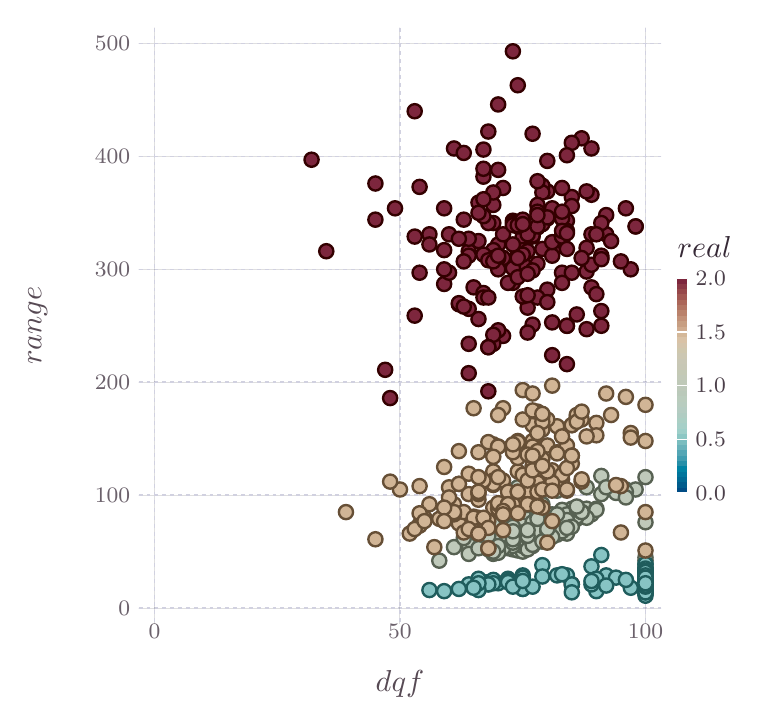
\begin{tikzpicture}[x=1mm,y=-1mm]
\definecolor{mycolorA5CFC7}{rgb}{0.65,0.81,0.78}
\definecolor{mycolor0083A3}{rgb}{0,0.51,0.64}
\definecolor{mycolorB7CBBF}{rgb}{0.72,0.8,0.75}
\definecolor{mycolor88C4C4}{rgb}{0.53,0.77,0.77}
\definecolor{mycolor7BBCC0}{rgb}{0.48,0.74,0.75}
\definecolor{mycolorAA665A}{rgb}{0.67,0.4,0.35}
\definecolor{mycolor664F35}{rgb}{0.4,0.31,0.21}
\definecolor{mycolorD2B497}{rgb}{0.82,0.71,0.59}
\definecolor{mycolorB27563}{rgb}{0.7,0.46,0.39}
\definecolor{mycolor1E5C5C}{rgb}{0.12,0.36,0.36}
\definecolor{mycolorC4C9B6}{rgb}{0.77,0.79,0.71}
\definecolor{mycolorC6C8B5}{rgb}{0.78,0.78,0.71}
\definecolor{mycolorBBCBBB}{rgb}{0.73,0.79,0.73}
\definecolor{mycolor96484A}{rgb}{0.59,0.28,0.29}
\definecolor{mycolor564A55}{rgb}{0.34,0.29,0.33}
\definecolor{mycolor004D84}{rgb}{0,0.3,0.52}
\definecolor{mycolor7E273E}{rgb}{0.49,0.15,0.24}
\definecolor{mycolor4C404B}{rgb}{0.3,0.25,0.29}
\definecolor{mycolorB1CCC2}{rgb}{0.69,0.8,0.76}
\definecolor{mycolor005B8D}{rgb}{0,0.36,0.55}
\definecolor{mycolorA05752}{rgb}{0.63,0.34,0.32}
\definecolor{mycolorC19177}{rgb}{0.76,0.57,0.47}
\definecolor{mycolorB5CCC1}{rgb}{0.71,0.8,0.76}
\definecolor{mycolorC89E82}{rgb}{0.78,0.62,0.51}
\definecolor{mycolorBA836C}{rgb}{0.73,0.51,0.42}
\definecolor{mycolorBFCAB8}{rgb}{0.75,0.79,0.72}
\definecolor{mycolorC9C7B4}{rgb}{0.79,0.78,0.71}
\definecolor{mycolorBECAB9}{rgb}{0.75,0.79,0.73}
\definecolor{mycolor8DC6C5}{rgb}{0.55,0.78,0.77}
\definecolor{mycolor000000}{rgb}{0,0,0}
\definecolor{mycolorCDAB8E}{rgb}{0.81,0.67,0.56}
\definecolor{mycolorD3B79A}{rgb}{0.83,0.72,0.6}
\definecolor{mycolor69B2BA}{rgb}{0.41,0.7,0.73}
\definecolor{mycolorD4C5AA}{rgb}{0.83,0.77,0.67}
\definecolor{mycolorABCEC4}{rgb}{0.67,0.81,0.77}
\definecolor{mycolor340000}{rgb}{0.2,0,0}
\definecolor{mycolorFFFFFF}{rgb}{1,1,1}
\definecolor{mycolor006995}{rgb}{0,0.41,0.58}
\definecolor{mycolorB9CBBD}{rgb}{0.73,0.8,0.74}
\definecolor{mycolor278FA9}{rgb}{0.15,0.56,0.66}
\definecolor{mycolor6C606B}{rgb}{0.42,0.38,0.42}
\definecolor{mycolor000000}{rgb}{0,0,0}
\definecolor{mycolor8B3844}{rgb}{0.54,0.22,0.27}
\definecolor{mycolor7E273E}{rgb}{0.49,0.15,0.24}
\definecolor{mycolorD8C3A6}{rgb}{0.85,0.76,0.65}
\definecolor{mycolor362A35}{rgb}{0.21,0.16,0.21}
\definecolor{mycolor409BAF}{rgb}{0.25,0.61,0.69}
\definecolor{mycolorCCC7B2}{rgb}{0.8,0.78,0.7}
\definecolor{mycolor55A7B5}{rgb}{0.33,0.65,0.71}
\definecolor{mycolorD0D0E0}{rgb}{0.82,0.82,0.88}
\definecolor{mycolor9ED0CB}{rgb}{0.62,0.81,0.79}
\definecolor{mycolor00769D}{rgb}{0,0.46,0.61}
\definecolor{mycolorC2C9B7}{rgb}{0.76,0.79,0.72}
\definecolor{mycolor576153}{rgb}{0.34,0.38,0.32}
\definecolor{mycolorBDCABA}{rgb}{0.74,0.79,0.73}
\definecolor{mycolorCFC6AE}{rgb}{0.81,0.78,0.68}
\begin{scope}
\begin{scope}
\draw (52.82,88.39) node [text=mycolor564A55,draw=mycolor000000,draw opacity=0,rotate around={-0: (0,1.81)},inner sep=0.0]{\fontsize{3.88mm}{4.66mm}\selectfont $\text{dqf}$};
\end{scope}
\begin{scope}
\draw (21.63,81.72) node [text=mycolor6C606B,rotate around={-0: (31.18,1.34)},inner sep=0.0]{\fontsize{2.82mm}{3.39mm}\selectfont $\text{0}$};
\draw (52.82,81.72) node [text=mycolor6C606B,rotate around={-0: (0,1.34)},inner sep=0.0]{\fontsize{2.82mm}{3.39mm}\selectfont $\text{50}$};
\draw (84,81.72) node [text=mycolor6C606B,rotate around={-0: (-31.18,1.34)},inner sep=0.0]{\fontsize{2.82mm}{3.39mm}\selectfont $\text{100}$};
\end{scope}
\begin{scope}
\begin{scope}
\draw (90.31,43.64) node [text=mycolor4C404B,rotate around={-0: (4.5,6.83)},right,inner sep=0.0]{\fontsize{2.82mm}{3.39mm}\selectfont $\text{1.5}$};
\draw (90.31,50.47) node [text=mycolor4C404B,rotate around={-0: (4.5,0)},right,inner sep=0.0]{\fontsize{2.82mm}{3.39mm}\selectfont $\text{1.0}$};
\draw (90.31,36.81) node [text=mycolor4C404B,rotate around={-0: (4.5,13.66)},right,inner sep=0.0]{\fontsize{2.82mm}{3.39mm}\selectfont $\text{2.0}$};
\draw (90.31,64.13) node [text=mycolor4C404B,rotate around={-0: (4.5,-13.66)},right,inner sep=0.0]{\fontsize{2.82mm}{3.39mm}\selectfont $\text{0.0}$};
\draw (90.31,57.3) node [text=mycolor4C404B,rotate around={-0: (4.5,-6.83)},right,inner sep=0.0]{\fontsize{2.82mm}{3.39mm}\selectfont $\text{0.5}$};
\end{scope}
\begin{scope}
\path [fill=mycolor004D84,draw=mycolor000000,draw opacity=0] (88,63.44) rectangle +(1.31,0.68);
\path [fill=mycolor005B8D,draw=mycolor000000,draw opacity=0] (88,62.76) rectangle +(1.31,0.68);
\path [fill=mycolor006995,draw=mycolor000000,draw opacity=0] (88,62.08) rectangle +(1.31,0.68);
\path [fill=mycolor00769D,draw=mycolor000000,draw opacity=0] (88,61.39) rectangle +(1.31,0.68);
\path [fill=mycolor0083A3,draw=mycolor000000,draw opacity=0] (88,60.71) rectangle +(1.31,0.68);
\path [fill=mycolor278FA9,draw=mycolor000000,draw opacity=0] (88,60.03) rectangle +(1.31,0.68);
\path [fill=mycolor409BAF,draw=mycolor000000,draw opacity=0] (88,59.35) rectangle +(1.31,0.68);
\path [fill=mycolor55A7B5,draw=mycolor000000,draw opacity=0] (88,58.66) rectangle +(1.31,0.68);
\path [fill=mycolor69B2BA,draw=mycolor000000,draw opacity=0] (88,57.98) rectangle +(1.31,0.68);
\path [fill=mycolor7BBCC0,draw=mycolor000000,draw opacity=0] (88,57.3) rectangle +(1.31,0.68);
\path [fill=mycolor8DC6C5,draw=mycolor000000,draw opacity=0] (88,56.61) rectangle +(1.31,0.68);
\path [fill=mycolor9ED0CB,draw=mycolor000000,draw opacity=0] (88,55.93) rectangle +(1.31,0.68);
\path [fill=mycolorA5CFC7,draw=mycolor000000,draw opacity=0] (88,55.25) rectangle +(1.31,0.68);
\path [fill=mycolorABCEC4,draw=mycolor000000,draw opacity=0] (88,54.57) rectangle +(1.31,0.68);
\path [fill=mycolorB1CCC2,draw=mycolor000000,draw opacity=0] (88,53.88) rectangle +(1.31,0.68);
\path [fill=mycolorB5CCC1,draw=mycolor000000,draw opacity=0] (88,53.2) rectangle +(1.31,0.68);
\path [fill=mycolorB7CBBF,draw=mycolor000000,draw opacity=0] (88,52.52) rectangle +(1.31,0.68);
\path [fill=mycolorB9CBBD,draw=mycolor000000,draw opacity=0] (88,51.83) rectangle +(1.31,0.68);
\path [fill=mycolorBBCBBB,draw=mycolor000000,draw opacity=0] (88,51.15) rectangle +(1.31,0.68);
\path [fill=mycolorBDCABA,draw=mycolor000000,draw opacity=0] (88,50.47) rectangle +(1.31,0.68);
\path [fill=mycolorBFCAB8,draw=mycolor000000,draw opacity=0] (88,49.79) rectangle +(1.31,0.68);
\path [fill=mycolorC2C9B7,draw=mycolor000000,draw opacity=0] (88,49.1) rectangle +(1.31,0.68);
\path [fill=mycolorC4C9B6,draw=mycolor000000,draw opacity=0] (88,48.42) rectangle +(1.31,0.68);
\path [fill=mycolorC6C8B5,draw=mycolor000000,draw opacity=0] (88,47.74) rectangle +(1.31,0.68);
\path [fill=mycolorC9C7B4,draw=mycolor000000,draw opacity=0] (88,47.06) rectangle +(1.31,0.68);
\path [fill=mycolorCCC7B2,draw=mycolor000000,draw opacity=0] (88,46.37) rectangle +(1.31,0.68);
\path [fill=mycolorCFC6AE,draw=mycolor000000,draw opacity=0] (88,45.69) rectangle +(1.31,0.68);
\path [fill=mycolorD4C5AA,draw=mycolor000000,draw opacity=0] (88,45.01) rectangle +(1.31,0.68);
\path [fill=mycolorD8C3A6,draw=mycolor000000,draw opacity=0] (88,44.32) rectangle +(1.31,0.68);
\path [fill=mycolorD3B79A,draw=mycolor000000,draw opacity=0] (88,43.64) rectangle +(1.31,0.68);
\path [fill=mycolorCDAB8E,draw=mycolor000000,draw opacity=0] (88,42.96) rectangle +(1.31,0.68);
\path [fill=mycolorC89E82,draw=mycolor000000,draw opacity=0] (88,42.28) rectangle +(1.31,0.68);
\path [fill=mycolorC19177,draw=mycolor000000,draw opacity=0] (88,41.59) rectangle +(1.31,0.68);
\path [fill=mycolorBA836C,draw=mycolor000000,draw opacity=0] (88,40.91) rectangle +(1.31,0.68);
\path [fill=mycolorB27563,draw=mycolor000000,draw opacity=0] (88,40.23) rectangle +(1.31,0.68);
\path [fill=mycolorAA665A,draw=mycolor000000,draw opacity=0] (88,39.54) rectangle +(1.31,0.68);
\path [fill=mycolorA05752,draw=mycolor000000,draw opacity=0] (88,38.86) rectangle +(1.31,0.68);
\path [fill=mycolor96484A,draw=mycolor000000,draw opacity=0] (88,38.18) rectangle +(1.31,0.68);
\path [fill=mycolor8B3844,draw=mycolor000000,draw opacity=0] (88,37.5) rectangle +(1.31,0.68);
\path [fill=mycolor7E273E,draw=mycolor000000,draw opacity=0] (88,36.81) rectangle +(1.31,0.68);
\begin{scope}
[line width=0.2mm]
\path [fill=mycolor004D84,draw=mycolorFFFFFF]  (88,43.64) -- (89.31,43.64);
\path [fill=mycolor005B8D,draw=mycolorFFFFFF]  (88,50.47) -- (89.31,50.47);
\path [fill=mycolor006995,draw=mycolorFFFFFF]  (88,36.81) -- (89.31,36.81);
\path [fill=mycolor00769D,draw=mycolorFFFFFF]  (88,64.13) -- (89.31,64.13);
\path [fill=mycolor0083A3,draw=mycolorFFFFFF]  (88,57.3) -- (89.31,57.3);
\end{scope}
\end{scope}
\begin{scope}
\draw (88,32.81) node [text=mycolor362A35,draw=mycolor000000,draw opacity=0,rotate around={-0: (4.5,0.19)},right,inner sep=0.0]{\fontsize{3.88mm}{4.66mm}\selectfont $\text{real}$};
\end{scope}
\end{scope}
\begin{scope}
\clip  (19.63,5) -- (86,5) -- (86,80.72) -- (19.63,80.72);
\begin{scope}
\clip  (19.63,5) -- (86,5) -- (86,80.72) -- (19.63,80.72);
\path [fill=mycolor000000,fill opacity=0,draw=mycolor000000,draw opacity=0] (19.63,5) rectangle +(66.37,75.72);
\end{scope}
\begin{scope}
[dash pattern=on 0.5mm off 0.5mm,line width=0.2mm]
\path [fill=mycolor000000,draw=mycolorD0D0E0]  (19.63,78.72) -- (86,78.72);
\path [fill=mycolor000000,draw=mycolorD0D0E0]  (19.63,64.37) -- (86,64.37);
\path [fill=mycolor000000,draw=mycolorD0D0E0]  (19.63,50.03) -- (86,50.03);
\path [fill=mycolor000000,draw=mycolorD0D0E0]  (19.63,35.69) -- (86,35.69);
\path [fill=mycolor000000,draw=mycolorD0D0E0]  (19.63,21.34) -- (86,21.34);
\path [fill=mycolor000000,draw=mycolorD0D0E0]  (19.63,7) -- (86,7);
\end{scope}
\begin{scope}
[dash pattern=on 0.5mm off 0.5mm,line width=0.2mm]
\path [fill=mycolor000000,draw=mycolorD0D0E0]  (21.63,5) -- (21.63,80.72);
\path [fill=mycolor000000,draw=mycolorD0D0E0]  (52.82,5) -- (52.82,80.72);
\path [fill=mycolor000000,draw=mycolorD0D0E0]  (84,5) -- (84,80.72);
\end{scope}
\begin{scope}
\begin{scope}
\begin{scope}
[line width=0.3mm]
\path [fill=mycolorBECAB9,draw=mycolor576153] (69.66,68.67) circle [radius=0.9];
\path [fill=mycolorBECAB9,draw=mycolor576153] (76.52,66.09) circle [radius=0.9];
\path [fill=mycolorBECAB9,draw=mycolor576153] (72.15,67.96) circle [radius=0.9];
\path [fill=mycolorBECAB9,draw=mycolor576153] (74.64,68.24) circle [radius=0.9];
\path [fill=mycolorBECAB9,draw=mycolor576153] (69.03,69.97) circle [radius=0.9];
\path [fill=mycolorBECAB9,draw=mycolor576153] (80.26,64.09) circle [radius=0.9];
\path [fill=mycolorBECAB9,draw=mycolor576153] (70.9,69.39) circle [radius=0.9];
\path [fill=mycolorBECAB9,draw=mycolor576153] (66.54,68.96) circle [radius=0.9];
\path [fill=mycolorBECAB9,draw=mycolor576153] (65.91,68.24) circle [radius=0.9];
\path [fill=mycolorBECAB9,draw=mycolor576153] (61.55,70.97) circle [radius=0.9];
\path [fill=mycolorBECAB9,draw=mycolor576153] (67.16,70.54) circle [radius=0.9];
\path [fill=mycolorBECAB9,draw=mycolor576153] (72.15,67.1) circle [radius=0.9];
\path [fill=mycolorBECAB9,draw=mycolor576153] (73.4,68.1) circle [radius=0.9];
\path [fill=mycolorBECAB9,draw=mycolor576153] (71.53,68.82) circle [radius=0.9];
\path [fill=mycolorBECAB9,draw=mycolor576153] (62.17,70.97) circle [radius=0.9];
\path [fill=mycolorBECAB9,draw=mycolor576153] (74.64,67.1) circle [radius=0.9];
\path [fill=mycolorBECAB9,draw=mycolor576153] (71.53,68.24) circle [radius=0.9];
\path [fill=mycolorBECAB9,draw=mycolor576153] (69.03,71.11) circle [radius=0.9];
\path [fill=mycolorBECAB9,draw=mycolor576153] (67.16,71.26) circle [radius=0.9];
\path [fill=mycolorBECAB9,draw=mycolor576153] (65.91,68.67) circle [radius=0.9];
\path [fill=mycolorBECAB9,draw=mycolor576153] (66.54,70.25) circle [radius=0.9];
\path [fill=mycolorBECAB9,draw=mycolor576153] (74.64,66.67) circle [radius=0.9];
\path [fill=mycolorBECAB9,draw=mycolor576153] (77.14,66.81) circle [radius=0.9];
\path [fill=mycolorBECAB9,draw=mycolor576153] (72.15,68.96) circle [radius=0.9];
\path [fill=mycolorBECAB9,draw=mycolor576153] (69.66,70.83) circle [radius=0.9];
\path [fill=mycolorBECAB9,draw=mycolor576153] (72.77,67.96) circle [radius=0.9];
\path [fill=mycolorBECAB9,draw=mycolor576153] (70.28,68.96) circle [radius=0.9];
\path [fill=mycolorBECAB9,draw=mycolor576153] (62.79,70.54) circle [radius=0.9];
\path [fill=mycolorBECAB9,draw=mycolor576153] (74.02,67.1) circle [radius=0.9];
\path [fill=mycolorBECAB9,draw=mycolor576153] (65.91,68.67) circle [radius=0.9];
\path [fill=mycolorBECAB9,draw=mycolor576153] (66.54,69.82) circle [radius=0.9];
\path [fill=mycolorBECAB9,draw=mycolor576153] (64.67,71.83) circle [radius=0.9];
\path [fill=mycolorBECAB9,draw=mycolor576153] (84,72.69) circle [radius=0.9];
\path [fill=mycolorBECAB9,draw=mycolor576153] (74.02,67.67) circle [radius=0.9];
\path [fill=mycolorBECAB9,draw=mycolor576153] (74.02,67.53) circle [radius=0.9];
\path [fill=mycolorBECAB9,draw=mycolor576153] (67.78,71.4) circle [radius=0.9];
\path [fill=mycolorBECAB9,draw=mycolor576153] (73.4,66.52) circle [radius=0.9];
\path [fill=mycolorBECAB9,draw=mycolor576153] (65.91,69.39) circle [radius=0.9];
\path [fill=mycolorBECAB9,draw=mycolor576153] (70.28,69.82) circle [radius=0.9];
\path [fill=mycolorBECAB9,draw=mycolor576153] (68.41,71.54) circle [radius=0.9];
\path [fill=mycolorBECAB9,draw=mycolor576153] (65.29,70.97) circle [radius=0.9];
\path [fill=mycolorBECAB9,draw=mycolor576153] (73.4,67.96) circle [radius=0.9];
\path [fill=mycolorBECAB9,draw=mycolor576153] (59.68,70.97) circle [radius=0.9];
\path [fill=mycolorBECAB9,draw=mycolor576153] (72.15,68.1) circle [radius=0.9];
\path [fill=mycolorBECAB9,draw=mycolor576153] (69.03,68.96) circle [radius=0.9];
\path [fill=mycolorBECAB9,draw=mycolor576153] (64.04,70.54) circle [radius=0.9];
\path [fill=mycolorBECAB9,draw=mycolor576153] (84,67.81) circle [radius=0.9];
\path [fill=mycolorBECAB9,draw=mycolor576153] (72.77,67.38) circle [radius=0.9];
\path [fill=mycolorBECAB9,draw=mycolor576153] (67.78,68.39) circle [radius=0.9];
\path [fill=mycolorBECAB9,draw=mycolor576153] (66.54,69.25) circle [radius=0.9];
\path [fill=mycolorBECAB9,draw=mycolor576153] (69.66,67.67) circle [radius=0.9];
\path [fill=mycolorBECAB9,draw=mycolor576153] (78.39,64.23) circle [radius=0.9];
\path [fill=mycolorBECAB9,draw=mycolor576153] (70.9,65.95) circle [radius=0.9];
\path [fill=mycolorBECAB9,draw=mycolor576153] (65.29,70.97) circle [radius=0.9];
\path [fill=mycolorBECAB9,draw=mycolor576153] (65.29,70.54) circle [radius=0.9];
\path [fill=mycolorBECAB9,draw=mycolor576153] (68.41,69.11) circle [radius=0.9];
\path [fill=mycolorBECAB9,draw=mycolor576153] (70.9,69.82) circle [radius=0.9];
\path [fill=mycolorBECAB9,draw=mycolor576153] (76.52,63.37) circle [radius=0.9];
\path [fill=mycolorBECAB9,draw=mycolor576153] (71.53,68.39) circle [radius=0.9];
\path [fill=mycolorBECAB9,draw=mycolor576153] (69.66,70.4) circle [radius=0.9];
\path [fill=mycolorBECAB9,draw=mycolor576153] (81.51,63.65) circle [radius=0.9];
\path [fill=mycolorBECAB9,draw=mycolor576153] (72.77,63.51) circle [radius=0.9];
\path [fill=mycolorBECAB9,draw=mycolor576153] (69.66,70.4) circle [radius=0.9];
\path [fill=mycolorBECAB9,draw=mycolor576153] (74.64,66.38) circle [radius=0.9];
\path [fill=mycolorBECAB9,draw=mycolor576153] (67.78,66.52) circle [radius=0.9];
\path [fill=mycolorBECAB9,draw=mycolor576153] (70.28,68.67) circle [radius=0.9];
\path [fill=mycolorBECAB9,draw=mycolor576153] (75.27,67.38) circle [radius=0.9];
\path [fill=mycolorBECAB9,draw=mycolor576153] (72.15,67.38) circle [radius=0.9];
\path [fill=mycolorBECAB9,draw=mycolor576153] (66.54,71.11) circle [radius=0.9];
\path [fill=mycolorBECAB9,draw=mycolor576153] (65.29,69.25) circle [radius=0.9];
\path [fill=mycolorBECAB9,draw=mycolor576153] (71.53,68.82) circle [radius=0.9];
\path [fill=mycolorBECAB9,draw=mycolor576153] (73.4,68.39) circle [radius=0.9];
\path [fill=mycolorBECAB9,draw=mycolor576153] (69.66,68.1) circle [radius=0.9];
\path [fill=mycolorBECAB9,draw=mycolor576153] (72.15,68.82) circle [radius=0.9];
\path [fill=mycolorBECAB9,draw=mycolor576153] (65.29,67.53) circle [radius=0.9];
\path [fill=mycolorBECAB9,draw=mycolor576153] (70.28,68.1) circle [radius=0.9];
\path [fill=mycolorBECAB9,draw=mycolor576153] (72.15,67.81) circle [radius=0.9];
\path [fill=mycolorBECAB9,draw=mycolor576153] (65.91,67.96) circle [radius=0.9];
\path [fill=mycolorBECAB9,draw=mycolor576153] (77.76,66.09) circle [radius=0.9];
\path [fill=mycolorBECAB9,draw=mycolor576153] (74.02,68.53) circle [radius=0.9];
\path [fill=mycolorBECAB9,draw=mycolor576153] (82.75,63.65) circle [radius=0.9];
\path [fill=mycolorBECAB9,draw=mycolor576153] (71.53,66.81) circle [radius=0.9];
\path [fill=mycolorBECAB9,draw=mycolor576153] (67.16,70.54) circle [radius=0.9];
\path [fill=mycolorBECAB9,draw=mycolor576153] (72.15,68.39) circle [radius=0.9];
\path [fill=mycolorBECAB9,draw=mycolor576153] (72.77,68.39) circle [radius=0.9];
\path [fill=mycolorBECAB9,draw=mycolor576153] (74.64,66.95) circle [radius=0.9];
\path [fill=mycolorBECAB9,draw=mycolor576153] (74.02,66.67) circle [radius=0.9];
\path [fill=mycolorBECAB9,draw=mycolor576153] (71.53,68.39) circle [radius=0.9];
\path [fill=mycolorBECAB9,draw=mycolor576153] (78.39,61.93) circle [radius=0.9];
\path [fill=mycolorBECAB9,draw=mycolor576153] (77.76,66.24) circle [radius=0.9];
\path [fill=mycolorBECAB9,draw=mycolor576153] (68.41,70.83) circle [radius=0.9];
\path [fill=mycolorBECAB9,draw=mycolor576153] (81.51,63.94) circle [radius=0.9];
\path [fill=mycolorBECAB9,draw=mycolor576153] (70.9,70.25) circle [radius=0.9];
\path [fill=mycolorBECAB9,draw=mycolor576153] (67.78,68.67) circle [radius=0.9];
\path [fill=mycolorBECAB9,draw=mycolor576153] (68.41,68.67) circle [radius=0.9];
\path [fill=mycolorBECAB9,draw=mycolor576153] (66.54,70.11) circle [radius=0.9];
\path [fill=mycolorBECAB9,draw=mycolor576153] (81.51,64.66) circle [radius=0.9];
\path [fill=mycolorBECAB9,draw=mycolor576153] (69.66,67.53) circle [radius=0.9];
\path [fill=mycolorBECAB9,draw=mycolor576153] (65.91,68.82) circle [radius=0.9];
\path [fill=mycolorBECAB9,draw=mycolor576153] (72.77,68.1) circle [radius=0.9];
\path [fill=mycolorBECAB9,draw=mycolor576153] (74.64,66.09) circle [radius=0.9];
\path [fill=mycolorBECAB9,draw=mycolor576153] (79.01,63.37) circle [radius=0.9];
\path [fill=mycolorBECAB9,draw=mycolor576153] (70.9,68.39) circle [radius=0.9];
\path [fill=mycolorBECAB9,draw=mycolor576153] (64.67,68.1) circle [radius=0.9];
\path [fill=mycolorBECAB9,draw=mycolor576153] (84,62.08) circle [radius=0.9];
\path [fill=mycolorBECAB9,draw=mycolor576153] (75.89,67.1) circle [radius=0.9];
\path [fill=mycolorBECAB9,draw=mycolor576153] (74.64,67.53) circle [radius=0.9];
\path [fill=mycolorBECAB9,draw=mycolor576153] (71.53,66.81) circle [radius=0.9];
\path [fill=mycolorBECAB9,draw=mycolor576153] (74.64,67.81) circle [radius=0.9];
\path [fill=mycolorBECAB9,draw=mycolor576153] (62.79,69.97) circle [radius=0.9];
\path [fill=mycolorBECAB9,draw=mycolor576153] (62.17,71.11) circle [radius=0.9];
\path [fill=mycolorBECAB9,draw=mycolor576153] (61.55,70.68) circle [radius=0.9];
\path [fill=mycolorBECAB9,draw=mycolor576153] (70.28,68.82) circle [radius=0.9];
\path [fill=mycolorBECAB9,draw=mycolor576153] (69.03,71.26) circle [radius=0.9];
\path [fill=mycolorBECAB9,draw=mycolor576153] (70.28,70.25) circle [radius=0.9];
\path [fill=mycolorBECAB9,draw=mycolor576153] (64.67,70.11) circle [radius=0.9];
\path [fill=mycolorBECAB9,draw=mycolor576153] (70.28,69.97) circle [radius=0.9];
\path [fill=mycolorBECAB9,draw=mycolor576153] (70.28,69.97) circle [radius=0.9];
\path [fill=mycolorBECAB9,draw=mycolor576153] (74.02,69.25) circle [radius=0.9];
\path [fill=mycolorBECAB9,draw=mycolor576153] (67.78,67.67) circle [radius=0.9];
\path [fill=mycolorBECAB9,draw=mycolor576153] (60.92,69.82) circle [radius=0.9];
\path [fill=mycolorBECAB9,draw=mycolor576153] (73.4,68.67) circle [radius=0.9];
\path [fill=mycolorBECAB9,draw=mycolor576153] (72.77,69.39) circle [radius=0.9];
\path [fill=mycolorBECAB9,draw=mycolor576153] (67.78,63.37) circle [radius=0.9];
\path [fill=mycolorBECAB9,draw=mycolor576153] (69.66,69.25) circle [radius=0.9];
\path [fill=mycolorBECAB9,draw=mycolor576153] (68.41,69.11) circle [radius=0.9];
\path [fill=mycolorBECAB9,draw=mycolor576153] (74.02,67.38) circle [radius=0.9];
\path [fill=mycolorBECAB9,draw=mycolor576153] (69.03,69.25) circle [radius=0.9];
\path [fill=mycolorBECAB9,draw=mycolor576153] (69.66,66.67) circle [radius=0.9];
\path [fill=mycolorBECAB9,draw=mycolor576153] (72.15,67.67) circle [radius=0.9];
\path [fill=mycolorBECAB9,draw=mycolor576153] (68.41,69.39) circle [radius=0.9];
\path [fill=mycolorBECAB9,draw=mycolor576153] (67.78,68.67) circle [radius=0.9];
\path [fill=mycolorBECAB9,draw=mycolor576153] (73.4,67.1) circle [radius=0.9];
\path [fill=mycolorBECAB9,draw=mycolor576153] (72.77,63.8) circle [radius=0.9];
\path [fill=mycolorBECAB9,draw=mycolor576153] (69.66,69.11) circle [radius=0.9];
\path [fill=mycolorBECAB9,draw=mycolor576153] (76.52,67.24) circle [radius=0.9];
\path [fill=mycolorBECAB9,draw=mycolor576153] (75.27,67.1) circle [radius=0.9];
\path [fill=mycolorBECAB9,draw=mycolor576153] (72.15,66.81) circle [radius=0.9];
\path [fill=mycolorBECAB9,draw=mycolor576153] (72.15,68.39) circle [radius=0.9];
\path [fill=mycolorBECAB9,draw=mycolor576153] (64.67,71.54) circle [radius=0.9];
\path [fill=mycolorBECAB9,draw=mycolor576153] (67.16,69.11) circle [radius=0.9];
\path [fill=mycolorBECAB9,draw=mycolor576153] (69.03,68.82) circle [radius=0.9];
\path [fill=mycolorBECAB9,draw=mycolor576153] (69.03,67.38) circle [radius=0.9];
\path [fill=mycolorBECAB9,draw=mycolor576153] (67.16,70.83) circle [radius=0.9];
\path [fill=mycolorBECAB9,draw=mycolor576153] (65.91,71.11) circle [radius=0.9];
\path [fill=mycolorBECAB9,draw=mycolor576153] (64.04,71.26) circle [radius=0.9];
\path [fill=mycolorBECAB9,draw=mycolor576153] (72.77,67.1) circle [radius=0.9];
\path [fill=mycolorBECAB9,draw=mycolor576153] (74.02,68.39) circle [radius=0.9];
\path [fill=mycolorBECAB9,draw=mycolor576153] (69.03,68.82) circle [radius=0.9];
\path [fill=mycolorBECAB9,draw=mycolor576153] (74.02,66.81) circle [radius=0.9];
\path [fill=mycolorBECAB9,draw=mycolor576153] (69.03,69.11) circle [radius=0.9];
\path [fill=mycolorBECAB9,draw=mycolor576153] (70.28,67.96) circle [radius=0.9];
\path [fill=mycolorBECAB9,draw=mycolor576153] (70.28,66.81) circle [radius=0.9];
\path [fill=mycolorBECAB9,draw=mycolor576153] (70.9,65.52) circle [radius=0.9];
\path [fill=mycolorBECAB9,draw=mycolor576153] (67.16,70.4) circle [radius=0.9];
\path [fill=mycolorBECAB9,draw=mycolor576153] (70.28,68.39) circle [radius=0.9];
\path [fill=mycolorBECAB9,draw=mycolor576153] (73.4,68.53) circle [radius=0.9];
\path [fill=mycolorBECAB9,draw=mycolor576153] (75.89,66.52) circle [radius=0.9];
\path [fill=mycolorBECAB9,draw=mycolor576153] (61.55,71.83) circle [radius=0.9];
\path [fill=mycolorBECAB9,draw=mycolor576153] (69.66,70.68) circle [radius=0.9];
\path [fill=mycolorBECAB9,draw=mycolor576153] (64.67,69.54) circle [radius=0.9];
\path [fill=mycolorBECAB9,draw=mycolor576153] (70.28,68.1) circle [radius=0.9];
\path [fill=mycolorBECAB9,draw=mycolor576153] (65.29,71.69) circle [radius=0.9];
\path [fill=mycolorBECAB9,draw=mycolor576153] (68.41,68.24) circle [radius=0.9];
\path [fill=mycolorBECAB9,draw=mycolor576153] (69.66,67.81) circle [radius=0.9];
\path [fill=mycolorBECAB9,draw=mycolor576153] (62.79,71.11) circle [radius=0.9];
\path [fill=mycolorBECAB9,draw=mycolor576153] (72.77,68.82) circle [radius=0.9];
\path [fill=mycolorBECAB9,draw=mycolor576153] (73.4,66.24) circle [radius=0.9];
\path [fill=mycolorBECAB9,draw=mycolor576153] (73.4,68.96) circle [radius=0.9];
\path [fill=mycolorBECAB9,draw=mycolor576153] (84,72.26) circle [radius=0.9];
\path [fill=mycolorBECAB9,draw=mycolor576153] (74.02,66.81) circle [radius=0.9];
\path [fill=mycolorBECAB9,draw=mycolor576153] (75.27,66.09) circle [radius=0.9];
\path [fill=mycolorBECAB9,draw=mycolor576153] (65.29,70.83) circle [radius=0.9];
\path [fill=mycolorBECAB9,draw=mycolor576153] (57.81,72.69) circle [radius=0.9];
\path [fill=mycolorBECAB9,draw=mycolor576153] (70.9,69.11) circle [radius=0.9];
\path [fill=mycolorBECAB9,draw=mycolor576153] (70.9,69.25) circle [radius=0.9];
\path [fill=mycolorBECAB9,draw=mycolor576153] (71.53,67.67) circle [radius=0.9];
\path [fill=mycolorBECAB9,draw=mycolor576153] (75.89,66.52) circle [radius=0.9];
\path [fill=mycolorBECAB9,draw=mycolor576153] (70.28,69.11) circle [radius=0.9];
\path [fill=mycolorBECAB9,draw=mycolor576153] (74.02,67.53) circle [radius=0.9];
\path [fill=mycolorBECAB9,draw=mycolor576153] (71.53,68.96) circle [radius=0.9];
\path [fill=mycolorBECAB9,draw=mycolor576153] (68.41,69.11) circle [radius=0.9];
\path [fill=mycolorBECAB9,draw=mycolor576153] (70.28,66.81) circle [radius=0.9];
\path [fill=mycolorBECAB9,draw=mycolor576153] (72.15,67.38) circle [radius=0.9];
\path [fill=mycolorBECAB9,draw=mycolor576153] (64.67,71.54) circle [radius=0.9];
\path [fill=mycolorBECAB9,draw=mycolor576153] (70.9,70.25) circle [radius=0.9];
\path [fill=mycolorBECAB9,draw=mycolor576153] (75.27,65.81) circle [radius=0.9];
\path [fill=mycolorBECAB9,draw=mycolor576153] (69.03,69.54) circle [radius=0.9];
\path [fill=mycolorBECAB9,draw=mycolor576153] (72.15,69.68) circle [radius=0.9];
\path [fill=mycolorBECAB9,draw=mycolor576153] (67.16,69.97) circle [radius=0.9];
\path [fill=mycolorBECAB9,draw=mycolor576153] (67.16,68.39) circle [radius=0.9];
\path [fill=mycolorBECAB9,draw=mycolor576153] (84,73.55) circle [radius=0.9];
\path [fill=mycolorBECAB9,draw=mycolor576153] (74.64,68.39) circle [radius=0.9];
\path [fill=mycolorBECAB9,draw=mycolor576153] (69.03,68.82) circle [radius=0.9];
\path [fill=mycolorBECAB9,draw=mycolor576153] (74.02,68.53) circle [radius=0.9];
\path [fill=mycolorBECAB9,draw=mycolor576153] (64.04,69.54) circle [radius=0.9];
\path [fill=mycolorBECAB9,draw=mycolor576153] (70.28,67.38) circle [radius=0.9];
\path [fill=mycolorBECAB9,draw=mycolor576153] (67.16,68.96) circle [radius=0.9];
\path [fill=mycolorBECAB9,draw=mycolor576153] (72.77,66.81) circle [radius=0.9];
\path [fill=mycolorBECAB9,draw=mycolor576153] (71.53,68.67) circle [radius=0.9];
\path [fill=mycolor7E273E,draw=mycolor340000] (74.64,75.7) circle [radius=0.9];
\path [fill=mycolor7E273E,draw=mycolor340000] (76.52,35.97) circle [radius=0.9];
\path [fill=mycolor7E273E,draw=mycolor340000] (50.94,48.45) circle [radius=0.9];
\path [fill=mycolor7E273E,draw=mycolor340000] (79.01,31.24) circle [radius=0.9];
\path [fill=mycolor7E273E,draw=mycolor340000] (77.14,20.34) circle [radius=0.9];
\path [fill=mycolor7E273E,draw=mycolor340000] (70.28,30.38) circle [radius=0.9];
\path [fill=mycolor7E273E,draw=mycolor340000] (59.68,20.34) circle [radius=0.9];
\path [fill=mycolor7E273E,draw=mycolor340000] (64.04,51.18) circle [radius=0.9];
\path [fill=mycolor7E273E,draw=mycolor340000] (65.91,44.15) circle [radius=0.9];
\path [fill=mycolor7E273E,draw=mycolor340000] (75.27,41.42) circle [radius=0.9];
\path [fill=mycolor7E273E,draw=mycolor340000] (72.15,46.59) circle [radius=0.9];
\path [fill=mycolor7E273E,draw=mycolor340000] (82.13,35.69) circle [radius=0.9];
\path [fill=mycolor7E273E,draw=mycolor340000] (58.43,37.55) circle [radius=0.9];
\path [fill=mycolor7E273E,draw=mycolor340000] (75.89,19.05) circle [radius=0.9];
\path [fill=mycolor7E273E,draw=mycolor340000] (69.03,40.56) circle [radius=0.9];
\path [fill=mycolor7E273E,draw=mycolor340000] (77.14,37.98) circle [radius=0.9];
\path [fill=mycolor7E273E,draw=mycolor340000] (43.46,33.39) circle [radius=0.9];
\path [fill=mycolor7E273E,draw=mycolor340000] (72.77,32.82) circle [radius=0.9];
\path [fill=mycolor7E273E,draw=mycolor340000] (62.79,32.1) circle [radius=0.9];
\path [fill=mycolor7E273E,draw=mycolor340000] (68.41,34.83) circle [radius=0.9];
\path [fill=mycolor7E273E,draw=mycolor340000] (67.78,12.31) circle [radius=0.9];
\path [fill=mycolor7E273E,draw=mycolor340000] (61.55,33.39) circle [radius=0.9];
\path [fill=mycolor7E273E,draw=mycolor340000] (59.05,31.24) circle [radius=0.9];
\path [fill=mycolor7E273E,draw=mycolor340000] (55.31,36.12) circle [radius=0.9];
\path [fill=mycolor7E273E,draw=mycolor340000] (62.17,37.98) circle [radius=0.9];
\path [fill=mycolor7E273E,draw=mycolor340000] (71.53,25.79) circle [radius=0.9];
\path [fill=mycolor7E273E,draw=mycolor340000] (65.91,25.36) circle [radius=0.9];
\path [fill=mycolor7E273E,draw=mycolor340000] (62.79,42) circle [radius=0.9];
\path [fill=mycolor7E273E,draw=mycolor340000] (69.66,42.71) circle [radius=0.9];
\path [fill=mycolor7E273E,draw=mycolor340000] (79.01,28.8) circle [radius=0.9];
\path [fill=mycolor7E273E,draw=mycolor340000] (64.67,27.51) circle [radius=0.9];
\path [fill=mycolor7E273E,draw=mycolor340000] (74.64,19.62) circle [radius=0.9];
\path [fill=mycolor7E273E,draw=mycolor340000] (65.29,32.53) circle [radius=0.9];
\path [fill=mycolor7E273E,draw=mycolor340000] (69.66,31.53) circle [radius=0.9];
\path [fill=mycolor7E273E,draw=mycolor340000] (68.41,31.53) circle [radius=0.9];
\path [fill=mycolor7E273E,draw=mycolor340000] (68.41,33.25) circle [radius=0.9];
\path [fill=mycolor7E273E,draw=mycolor340000] (71.53,29.23) circle [radius=0.9];
\path [fill=mycolor7E273E,draw=mycolor340000] (77.14,31.24) circle [radius=0.9];
\path [fill=mycolor7E273E,draw=mycolor340000] (69.66,31.38) circle [radius=0.9];
\path [fill=mycolor7E273E,draw=mycolor340000] (67.16,29.52) circle [radius=0.9];
\path [fill=mycolor7E273E,draw=mycolor340000] (58.43,33.25) circle [radius=0.9];
\path [fill=mycolor7E273E,draw=mycolor340000] (64.67,29.81) circle [radius=0.9];
\path [fill=mycolor7E273E,draw=mycolor340000] (61.55,45.15) circle [radius=0.9];
\path [fill=mycolor7E273E,draw=mycolor340000] (67.16,29.81) circle [radius=0.9];
\path [fill=mycolor7E273E,draw=mycolor340000] (59.05,36.12) circle [radius=0.9];
\path [fill=mycolor7E273E,draw=mycolor340000] (61.55,33.96) circle [radius=0.9];
\path [fill=mycolor7E273E,draw=mycolor340000] (67.16,35.26) circle [radius=0.9];
\path [fill=mycolor7E273E,draw=mycolor340000] (49.7,29.38) circle [radius=0.9];
\path [fill=mycolor7E273E,draw=mycolor340000] (62.79,27.22) circle [radius=0.9];
\path [fill=mycolor7E273E,draw=mycolor340000] (73.4,29.23) circle [radius=0.9];
\path [fill=mycolor7E273E,draw=mycolor340000] (67.16,35.54) circle [radius=0.9];
\path [fill=mycolor7E273E,draw=mycolor340000] (65.29,14.75) circle [radius=0.9];
\path [fill=mycolor7E273E,draw=mycolor340000] (82.75,30.24) circle [radius=0.9];
\path [fill=mycolor7E273E,draw=mycolor340000] (70.28,34.97) circle [radius=0.9];
\path [fill=mycolor7E273E,draw=mycolor340000] (64.67,33.25) circle [radius=0.9];
\path [fill=mycolor7E273E,draw=mycolor340000] (64.67,25.93) circle [radius=0.9];
\path [fill=mycolor7E273E,draw=mycolor340000] (64.04,29.81) circle [radius=0.9];
\path [fill=mycolor7E273E,draw=mycolor340000] (70.9,25.07) circle [radius=0.9];
\path [fill=mycolor7E273E,draw=mycolor340000] (77.14,26.22) circle [radius=0.9];
\path [fill=mycolor7E273E,draw=mycolor340000] (70.9,25.93) circle [radius=0.9];
\path [fill=mycolor7E273E,draw=mycolor340000] (78.39,34.25) circle [radius=0.9];
\path [fill=mycolor7E273E,draw=mycolor340000] (70.28,27.51) circle [radius=0.9];
\path [fill=mycolor7E273E,draw=mycolor340000] (67.78,33.82) circle [radius=0.9];
\path [fill=mycolor7E273E,draw=mycolor340000] (69.03,31.24) circle [radius=0.9];
\path [fill=mycolor7E273E,draw=mycolor340000] (67.78,30.24) circle [radius=0.9];
\path [fill=mycolor7E273E,draw=mycolor340000] (71.53,38.27) circle [radius=0.9];
\path [fill=mycolor7E273E,draw=mycolor340000] (74.64,26.51) circle [radius=0.9];
\path [fill=mycolor7E273E,draw=mycolor340000] (74.02,29.52) circle [radius=0.9];
\path [fill=mycolor7E273E,draw=mycolor340000] (70.9,29.95) circle [radius=0.9];
\path [fill=mycolor7E273E,draw=mycolor340000] (70.28,28.37) circle [radius=0.9];
\path [fill=mycolor7E273E,draw=mycolor340000] (73.4,36.12) circle [radius=0.9];
\path [fill=mycolor7E273E,draw=mycolor340000] (79.63,32.1) circle [radius=0.9];
\path [fill=mycolor7E273E,draw=mycolor340000] (81.51,27.94) circle [radius=0.9];
\path [fill=mycolor7E273E,draw=mycolor340000] (67.78,29.81) circle [radius=0.9];
\path [fill=mycolor7E273E,draw=mycolor340000] (70.9,33.1) circle [radius=0.9];
\path [fill=mycolor7E273E,draw=mycolor340000] (70.28,24.5) circle [radius=0.9];
\path [fill=mycolor7E273E,draw=mycolor340000] (76.52,25.79) circle [radius=0.9];
\path [fill=mycolor7E273E,draw=mycolor340000] (72.15,27.94) circle [radius=0.9];
\path [fill=mycolor7E273E,draw=mycolor340000] (71.53,29.09) circle [radius=0.9];
\path [fill=mycolor7E273E,draw=mycolor340000] (70.28,30.24) circle [radius=0.9];
\path [fill=mycolor7E273E,draw=mycolor340000] (77.14,35.11) circle [radius=0.9];
\path [fill=mycolor7E273E,draw=mycolor340000] (73.4,25.36) circle [radius=0.9];
\path [fill=mycolor7E273E,draw=mycolor340000] (74.02,21.2) circle [radius=0.9];
\path [fill=mycolor7E273E,draw=mycolor340000] (63.42,23.92) circle [radius=0.9];
\path [fill=mycolor7E273E,draw=mycolor340000] (60.92,29.38) circle [radius=0.9];
\path [fill=mycolor7E273E,draw=mycolor340000] (63.42,20.48) circle [radius=0.9];
\path [fill=mycolor7E273E,draw=mycolor340000] (65.91,31.24) circle [radius=0.9];
\path [fill=mycolor7E273E,draw=mycolor340000] (70.28,28.8) circle [radius=0.9];
\path [fill=mycolor7E273E,draw=mycolor340000] (73.4,29.23) circle [radius=0.9];
\path [fill=mycolor7E273E,draw=mycolor340000] (67.16,30.09) circle [radius=0.9];
\path [fill=mycolor7E273E,draw=mycolor340000] (68.41,29.81) circle [radius=0.9];
\path [fill=mycolor7E273E,draw=mycolor340000] (82.75,30.24) circle [radius=0.9];
\path [fill=mycolor7E273E,draw=mycolor340000] (71.53,21.92) circle [radius=0.9];
\path [fill=mycolor7E273E,draw=mycolor340000] (69.03,33.39) circle [radius=0.9];
\path [fill=mycolor7E273E,draw=mycolor340000] (74.02,30.81) circle [radius=0.9];
\path [fill=mycolor7E273E,draw=mycolor340000] (64.67,34.25) circle [radius=0.9];
\path [fill=mycolor7E273E,draw=mycolor340000] (56.56,31.24) circle [radius=0.9];
\path [fill=mycolor7E273E,draw=mycolor340000] (49.7,24.79) circle [radius=0.9];
\path [fill=mycolor7E273E,draw=mycolor340000] (41.59,21.77) circle [radius=0.9];
\path [fill=mycolor7E273E,draw=mycolor340000] (68.41,33.82) circle [radius=0.9];
\path [fill=mycolor7E273E,draw=mycolor340000] (54.69,31.53) circle [radius=0.9];
\path [fill=mycolor7E273E,draw=mycolor340000] (51.57,52.04) circle [radius=0.9];
\path [fill=mycolor7E273E,draw=mycolor340000] (67.16,37.41) circle [radius=0.9];
\path [fill=mycolor7E273E,draw=mycolor340000] (64.04,18.19) circle [radius=0.9];
\path [fill=mycolor7E273E,draw=mycolor340000] (69.03,43.72) circle [radius=0.9];
\path [fill=mycolor7E273E,draw=mycolor340000] (61.55,31.81) circle [radius=0.9];
\path [fill=mycolor7E273E,draw=mycolor340000] (74.64,27.65) circle [radius=0.9];
\path [fill=mycolor7E273E,draw=mycolor340000] (55.31,25.22) circle [radius=0.9];
\path [fill=mycolor7E273E,draw=mycolor340000] (70.28,39.27) circle [radius=0.9];
\path [fill=mycolor7E273E,draw=mycolor340000] (68.41,39.13) circle [radius=0.9];
\path [fill=mycolor7E273E,draw=mycolor340000] (65.29,23.06) circle [radius=0.9];
\path [fill=mycolor7E273E,draw=mycolor340000] (78.39,33.96) circle [radius=0.9];
\path [fill=mycolor7E273E,draw=mycolor340000] (63.42,28.94) circle [radius=0.9];
\path [fill=mycolor7E273E,draw=mycolor340000] (78.39,29.81) circle [radius=0.9];
\path [fill=mycolor7E273E,draw=mycolor340000] (67.16,8) circle [radius=0.9];
\path [fill=mycolor7E273E,draw=mycolor340000] (78.39,42.86) circle [radius=0.9];
\path [fill=mycolor7E273E,draw=mycolor340000] (76.52,43.29) circle [radius=0.9];
\path [fill=mycolor7E273E,draw=mycolor340000] (76.52,32.96) circle [radius=0.9];
\path [fill=mycolor7E273E,draw=mycolor340000] (60.3,40.13) circle [radius=0.9];
\path [fill=mycolor7E273E,draw=mycolor340000] (67.78,30.09) circle [radius=0.9];
\path [fill=mycolor7E273E,draw=mycolor340000] (66.54,37.41) circle [radius=0.9];
\path [fill=mycolor7E273E,draw=mycolor340000] (78.39,34.4) circle [radius=0.9];
\path [fill=mycolor7E273E,draw=mycolor340000] (67.16,32.53) circle [radius=0.9];
\path [fill=mycolor7E273E,draw=mycolor340000] (69.03,38.98) circle [radius=0.9];
\path [fill=mycolor7E273E,draw=mycolor340000] (69.66,18.47) circle [radius=0.9];
\path [fill=mycolor7E273E,draw=mycolor340000] (62.79,28.51) circle [radius=0.9];
\path [fill=mycolor7E273E,draw=mycolor340000] (64.67,45.15) circle [radius=0.9];
\path [fill=mycolor7E273E,draw=mycolor340000] (67.78,34.25) circle [radius=0.9];
\path [fill=mycolor7E273E,draw=mycolor340000] (63.42,33.82) circle [radius=0.9];
\path [fill=mycolor7E273E,draw=mycolor340000] (77.76,31.24) circle [radius=0.9];
\path [fill=mycolor7E273E,draw=mycolor340000] (75.89,34.25) circle [radius=0.9];
\path [fill=mycolor7E273E,draw=mycolor340000] (69.66,35.83) circle [radius=0.9];
\path [fill=mycolor7E273E,draw=mycolor340000] (74.64,36.12) circle [radius=0.9];
\path [fill=mycolor7E273E,draw=mycolor340000] (73.4,32.1) circle [radius=0.9];
\path [fill=mycolor7E273E,draw=mycolor340000] (73.4,37.41) circle [radius=0.9];
\path [fill=mycolor7E273E,draw=mycolor340000] (61.55,40.71) circle [radius=0.9];
\path [fill=mycolor7E273E,draw=mycolor340000] (60.3,39.99) circle [radius=0.9];
\path [fill=mycolor7E273E,draw=mycolor340000] (72.15,42.43) circle [radius=0.9];
\path [fill=mycolor7E273E,draw=mycolor340000] (67.78,36.69) circle [radius=0.9];
\path [fill=mycolor7E273E,draw=mycolor340000] (73.4,28.37) circle [radius=0.9];
\path [fill=mycolor7E273E,draw=mycolor340000] (64.04,34.54) circle [radius=0.9];
\path [fill=mycolor7E273E,draw=mycolor340000] (72.15,33.96) circle [radius=0.9];
\path [fill=mycolor7E273E,draw=mycolor340000] (54.69,41.57) circle [radius=0.9];
\path [fill=mycolor7E273E,draw=mycolor340000] (65.29,43.43) circle [radius=0.9];
\path [fill=mycolor7E273E,draw=mycolor340000] (65.91,34.25) circle [radius=0.9];
\path [fill=mycolor7E273E,draw=mycolor340000] (65.91,34.25) circle [radius=0.9];
\path [fill=mycolor7E273E,draw=mycolor340000] (65.29,34.25) circle [radius=0.9];
\path [fill=mycolor7E273E,draw=mycolor340000] (65.29,35.69) circle [radius=0.9];
\path [fill=mycolor7E273E,draw=mycolor340000] (63.42,38.7) circle [radius=0.9];
\path [fill=mycolor7E273E,draw=mycolor340000] (60.3,31.81) circle [radius=0.9];
\path [fill=mycolor7E273E,draw=mycolor340000] (63.42,26.79) circle [radius=0.9];
\path [fill=mycolor7E273E,draw=mycolor340000] (68.41,29.38) circle [radius=0.9];
\path [fill=mycolor7E273E,draw=mycolor340000] (64.67,34.68) circle [radius=0.9];
\path [fill=mycolor7E273E,draw=mycolor340000] (58.43,35.69) circle [radius=0.9];
\path [fill=mycolor7E273E,draw=mycolor340000] (72.15,32.24) circle [radius=0.9];
\path [fill=mycolor7E273E,draw=mycolor340000] (77.76,38.84) circle [radius=0.9];
\path [fill=mycolor7E273E,draw=mycolor340000] (63.42,39.27) circle [radius=0.9];
\path [fill=mycolor7E273E,draw=mycolor340000] (73.4,31.53) circle [radius=0.9];
\path [fill=mycolor7E273E,draw=mycolor340000] (73.4,31.53) circle [radius=0.9];
\path [fill=mycolor7E273E,draw=mycolor340000] (64.67,44) circle [radius=0.9];
\path [fill=mycolor7E273E,draw=mycolor340000] (80.88,34.68) circle [radius=0.9];
\path [fill=mycolor7E273E,draw=mycolor340000] (74.02,33.1) circle [radius=0.9];
\path [fill=mycolor7E273E,draw=mycolor340000] (60.92,20.91) circle [radius=0.9];
\path [fill=mycolor7E273E,draw=mycolor340000] (60.92,40.42) circle [radius=0.9];
\path [fill=mycolor7E273E,draw=mycolor340000] (73.4,30.81) circle [radius=0.9];
\path [fill=mycolor7E273E,draw=mycolor340000] (64.04,45.58) circle [radius=0.9];
\path [fill=mycolor7E273E,draw=mycolor340000] (64.04,45.58) circle [radius=0.9];
\path [fill=mycolor7E273E,draw=mycolor340000] (61.55,48.88) circle [radius=0.9];
\path [fill=mycolor7E273E,draw=mycolor340000] (71.53,39.85) circle [radius=0.9];
\path [fill=mycolor7E273E,draw=mycolor340000] (60.92,34.68) circle [radius=0.9];
\path [fill=mycolor7E273E,draw=mycolor340000] (74.02,42.86) circle [radius=0.9];
\path [fill=mycolor7E273E,draw=mycolor340000] (74.02,42.86) circle [radius=0.9];
\path [fill=mycolor7E273E,draw=mycolor340000] (58.43,27.94) circle [radius=0.9];
\path [fill=mycolor7E273E,draw=mycolor340000] (69.03,36.26) circle [radius=0.9];
\path [fill=mycolor7E273E,draw=mycolor340000] (63.42,22.92) circle [radius=0.9];
\path [fill=mycolor7E273E,draw=mycolor340000] (64.04,39.27) circle [radius=0.9];
\path [fill=mycolor7E273E,draw=mycolor340000] (52.19,27.94) circle [radius=0.9];
\path [fill=mycolor7E273E,draw=mycolor340000] (78.39,40.99) circle [radius=0.9];
\path [fill=mycolor7E273E,draw=mycolor340000] (74.02,47.73) circle [radius=0.9];
\path [fill=mycolor7E273E,draw=mycolor340000] (54.69,15.61) circle [radius=0.9];
\path [fill=mycolor7E273E,draw=mycolor340000] (65.29,33.96) circle [radius=0.9];
\path [fill=mycolor7E273E,draw=mycolor340000] (74.02,31.1) circle [radius=0.9];
\path [fill=mycolor7E273E,draw=mycolor340000] (56.56,32.53) circle [radius=0.9];
\path [fill=mycolor7E273E,draw=mycolor340000] (68.41,29.95) circle [radius=0.9];
\path [fill=mycolor88C4C4,draw=mycolor1E5C5C] (70.9,73.26) circle [radius=0.9];
\path [fill=mycolor88C4C4,draw=mycolor1E5C5C] (70.9,74.7) circle [radius=0.9];
\path [fill=mycolor88C4C4,draw=mycolor1E5C5C] (84,75.27) circle [radius=0.9];
\path [fill=mycolor88C4C4,draw=mycolor1E5C5C] (65.29,75.56) circle [radius=0.9];
\path [fill=mycolor88C4C4,draw=mycolor1E5C5C] (61.55,75.7) circle [radius=0.9];
\path [fill=mycolor88C4C4,draw=mycolor1E5C5C] (79.01,74.56) circle [radius=0.9];
\path [fill=mycolor88C4C4,draw=mycolor1E5C5C] (84,76.42) circle [radius=0.9];
\path [fill=mycolor88C4C4,draw=mycolor1E5C5C] (64.04,75.42) circle [radius=0.9];
\path [fill=mycolor88C4C4,draw=mycolor1E5C5C] (60.3,76.28) circle [radius=0.9];
\path [fill=mycolor88C4C4,draw=mycolor1E5C5C] (78.39,71.97) circle [radius=0.9];
\path [fill=mycolor88C4C4,draw=mycolor1E5C5C] (84,76.42) circle [radius=0.9];
\path [fill=mycolor88C4C4,draw=mycolor1E5C5C] (68.41,74.56) circle [radius=0.9];
\path [fill=mycolor88C4C4,draw=mycolor1E5C5C] (77.14,73.41) circle [radius=0.9];
\path [fill=mycolor88C4C4,draw=mycolor1E5C5C] (63.42,75.42) circle [radius=0.9];
\path [fill=mycolor88C4C4,draw=mycolor1E5C5C] (66.54,75.27) circle [radius=0.9];
\path [fill=mycolor88C4C4,draw=mycolor1E5C5C] (72.77,74.56) circle [radius=0.9];
\path [fill=mycolor88C4C4,draw=mycolor1E5C5C] (66.54,74.99) circle [radius=0.9];
\path [fill=mycolor88C4C4,draw=mycolor1E5C5C] (77.76,75.13) circle [radius=0.9];
\path [fill=mycolor88C4C4,draw=mycolor1E5C5C] (84,73.98) circle [radius=0.9];
\path [fill=mycolor88C4C4,draw=mycolor1E5C5C] (84,73.12) circle [radius=0.9];
\path [fill=mycolor88C4C4,draw=mycolor1E5C5C] (77.76,76.56) circle [radius=0.9];
\path [fill=mycolor88C4C4,draw=mycolor1E5C5C] (84,76.42) circle [radius=0.9];
\path [fill=mycolor88C4C4,draw=mycolor1E5C5C] (84,75.13) circle [radius=0.9];
\path [fill=mycolor88C4C4,draw=mycolor1E5C5C] (66.54,75.27) circle [radius=0.9];
\path [fill=mycolor88C4C4,draw=mycolor1E5C5C] (68.41,76.28) circle [radius=0.9];
\path [fill=mycolor88C4C4,draw=mycolor1E5C5C] (68.41,74.84) circle [radius=0.9];
\path [fill=mycolor88C4C4,draw=mycolor1E5C5C] (84,76.42) circle [radius=0.9];
\path [fill=mycolor88C4C4,draw=mycolor1E5C5C] (64.04,75.7) circle [radius=0.9];
\path [fill=mycolor88C4C4,draw=mycolor1E5C5C] (84,73.84) circle [radius=0.9];
\path [fill=mycolor88C4C4,draw=mycolor1E5C5C] (68.41,76.28) circle [radius=0.9];
\path [fill=mycolor88C4C4,draw=mycolor1E5C5C] (69.66,75.99) circle [radius=0.9];
\path [fill=mycolor88C4C4,draw=mycolor1E5C5C] (62.79,74.99) circle [radius=0.9];
\path [fill=mycolor88C4C4,draw=mycolor1E5C5C] (84,75.27) circle [radius=0.9];
\path [fill=mycolor88C4C4,draw=mycolor1E5C5C] (84,73.69) circle [radius=0.9];
\path [fill=mycolor88C4C4,draw=mycolor1E5C5C] (64.67,75.13) circle [radius=0.9];
\path [fill=mycolor88C4C4,draw=mycolor1E5C5C] (84,73.98) circle [radius=0.9];
\path [fill=mycolor88C4C4,draw=mycolor1E5C5C] (84,73.98) circle [radius=0.9];
\path [fill=mycolor88C4C4,draw=mycolor1E5C5C] (84,75.13) circle [radius=0.9];
\path [fill=mycolor88C4C4,draw=mycolor1E5C5C] (84,74.99) circle [radius=0.9];
\path [fill=mycolor88C4C4,draw=mycolor1E5C5C] (64.67,75.56) circle [radius=0.9];
\path [fill=mycolor88C4C4,draw=mycolor1E5C5C] (84,73.98) circle [radius=0.9];
\path [fill=mycolor88C4C4,draw=mycolor1E5C5C] (84,74.84) circle [radius=0.9];
\path [fill=mycolor88C4C4,draw=mycolor1E5C5C] (84,76.85) circle [radius=0.9];
\path [fill=mycolor88C4C4,draw=mycolor1E5C5C] (77.76,75.13) circle [radius=0.9];
\path [fill=mycolor88C4C4,draw=mycolor1E5C5C] (66.54,75.42) circle [radius=0.9];
\path [fill=mycolor88C4C4,draw=mycolor1E5C5C] (74.02,74.56) circle [radius=0.9];
\path [fill=mycolor88C4C4,draw=mycolor1E5C5C] (84,73.12) circle [radius=0.9];
\path [fill=mycolor88C4C4,draw=mycolor1E5C5C] (84,74.99) circle [radius=0.9];
\path [fill=mycolor88C4C4,draw=mycolor1E5C5C] (84,74.41) circle [radius=0.9];
\path [fill=mycolor88C4C4,draw=mycolor1E5C5C] (84,75.13) circle [radius=0.9];
\path [fill=mycolor88C4C4,draw=mycolor1E5C5C] (67.16,75.99) circle [radius=0.9];
\path [fill=mycolor88C4C4,draw=mycolor1E5C5C] (84,76.71) circle [radius=0.9];
\path [fill=mycolor88C4C4,draw=mycolor1E5C5C] (84,75.13) circle [radius=0.9];
\path [fill=mycolor88C4C4,draw=mycolor1E5C5C] (77.14,75.7) circle [radius=0.9];
\path [fill=mycolor88C4C4,draw=mycolor1E5C5C] (84,73.98) circle [radius=0.9];
\path [fill=mycolor88C4C4,draw=mycolor1E5C5C] (84,75.27) circle [radius=0.9];
\path [fill=mycolor88C4C4,draw=mycolor1E5C5C] (84,74.13) circle [radius=0.9];
\path [fill=mycolor88C4C4,draw=mycolor1E5C5C] (80.26,74.84) circle [radius=0.9];
\path [fill=mycolor88C4C4,draw=mycolor1E5C5C] (74.64,75.7) circle [radius=0.9];
\path [fill=mycolor88C4C4,draw=mycolor1E5C5C] (64.04,75.7) circle [radius=0.9];
\path [fill=mycolor88C4C4,draw=mycolor1E5C5C] (62.79,76.42) circle [radius=0.9];
\path [fill=mycolor88C4C4,draw=mycolor1E5C5C] (82.13,76.13) circle [radius=0.9];
\path [fill=mycolor88C4C4,draw=mycolor1E5C5C] (84,76.71) circle [radius=0.9];
\path [fill=mycolor88C4C4,draw=mycolor1E5C5C] (84,75.13) circle [radius=0.9];
\path [fill=mycolor88C4C4,draw=mycolor1E5C5C] (81.51,75.13) circle [radius=0.9];
\path [fill=mycolor88C4C4,draw=mycolor1E5C5C] (84,73.69) circle [radius=0.9];
\path [fill=mycolor88C4C4,draw=mycolor1E5C5C] (84,76.42) circle [radius=0.9];
\path [fill=mycolor88C4C4,draw=mycolor1E5C5C] (84,74.13) circle [radius=0.9];
\path [fill=mycolor88C4C4,draw=mycolor1E5C5C] (58.43,76.56) circle [radius=0.9];
\path [fill=mycolor88C4C4,draw=mycolor1E5C5C] (84,77.14) circle [radius=0.9];
\path [fill=mycolor88C4C4,draw=mycolor1E5C5C] (84,74.99) circle [radius=0.9];
\path [fill=mycolor88C4C4,draw=mycolor1E5C5C] (84,76.71) circle [radius=0.9];
\path [fill=mycolor88C4C4,draw=mycolor1E5C5C] (73.4,74.41) circle [radius=0.9];
\path [fill=mycolor88C4C4,draw=mycolor1E5C5C] (84,76.42) circle [radius=0.9];
\path [fill=mycolor88C4C4,draw=mycolor1E5C5C] (84,74.13) circle [radius=0.9];
\path [fill=mycolor88C4C4,draw=mycolor1E5C5C] (84,75.27) circle [radius=0.9];
\path [fill=mycolor88C4C4,draw=mycolor1E5C5C] (84,74.99) circle [radius=0.9];
\path [fill=mycolor88C4C4,draw=mycolor1E5C5C] (56.56,76.42) circle [radius=0.9];
\path [fill=mycolor88C4C4,draw=mycolor1E5C5C] (84,75.27) circle [radius=0.9];
\path [fill=mycolor88C4C4,draw=mycolor1E5C5C] (68.41,75.27) circle [radius=0.9];
\path [fill=mycolor88C4C4,draw=mycolor1E5C5C] (77.76,74.99) circle [radius=0.9];
\path [fill=mycolor88C4C4,draw=mycolor1E5C5C] (79.01,75.85) circle [radius=0.9];
\path [fill=mycolor88C4C4,draw=mycolor1E5C5C] (62.79,75.56) circle [radius=0.9];
\path [fill=mycolor88C4C4,draw=mycolor1E5C5C] (62.17,76.13) circle [radius=0.9];
\path [fill=mycolor88C4C4,draw=mycolor1E5C5C] (84,73.98) circle [radius=0.9];
\path [fill=mycolor88C4C4,draw=mycolor1E5C5C] (84,76.42) circle [radius=0.9];
\path [fill=mycolor88C4C4,draw=mycolor1E5C5C] (84,75.13) circle [radius=0.9];
\path [fill=mycolor88C4C4,draw=mycolor1E5C5C] (84,74.13) circle [radius=0.9];
\path [fill=mycolor88C4C4,draw=mycolor1E5C5C] (77.14,75.27) circle [radius=0.9];
\path [fill=mycolor88C4C4,draw=mycolor1E5C5C] (74.64,76.71) circle [radius=0.9];
\path [fill=mycolor88C4C4,draw=mycolor1E5C5C] (84,75.42) circle [radius=0.9];
\path [fill=mycolor88C4C4,draw=mycolor1E5C5C] (84,75.85) circle [radius=0.9];
\path [fill=mycolor88C4C4,draw=mycolor1E5C5C] (84,76.71) circle [radius=0.9];
\path [fill=mycolor88C4C4,draw=mycolor1E5C5C] (84,75.7) circle [radius=0.9];
\path [fill=mycolor88C4C4,draw=mycolor1E5C5C] (84,74.56) circle [radius=0.9];
\path [fill=mycolor88C4C4,draw=mycolor1E5C5C] (84,75.27) circle [radius=0.9];
\path [fill=mycolor88C4C4,draw=mycolor1E5C5C] (84,75.99) circle [radius=0.9];
\path [fill=mycolor88C4C4,draw=mycolor1E5C5C] (84,75.85) circle [radius=0.9];
\path [fill=mycolor88C4C4,draw=mycolor1E5C5C] (84,74.99) circle [radius=0.9];
\path [fill=mycolor88C4C4,draw=mycolor1E5C5C] (84,75.42) circle [radius=0.9];
\path [fill=mycolor88C4C4,draw=mycolor1E5C5C] (84,75.42) circle [radius=0.9];
\path [fill=mycolor88C4C4,draw=mycolor1E5C5C] (84,74.84) circle [radius=0.9];
\path [fill=mycolor88C4C4,draw=mycolor1E5C5C] (84,75.56) circle [radius=0.9];
\path [fill=mycolorD2B497,draw=mycolor664F35] (75.89,62.65) circle [radius=0.9];
\path [fill=mycolorD2B497,draw=mycolor664F35] (77.76,55.19) circle [radius=0.9];
\path [fill=mycolorD2B497,draw=mycolor664F35] (64.67,57.92) circle [radius=0.9];
\path [fill=mycolorD2B497,draw=mycolor664F35] (79.01,51.46) circle [radius=0.9];
\path [fill=mycolorD2B497,draw=mycolor664F35] (72.77,55.62) circle [radius=0.9];
\path [fill=mycolorD2B497,draw=mycolor664F35] (61.55,64.23) circle [radius=0.9];
\path [fill=mycolorD2B497,draw=mycolor664F35] (67.16,58.35) circle [radius=0.9];
\path [fill=mycolorD2B497,draw=mycolor664F35] (60.3,62.94) circle [radius=0.9];
\path [fill=mycolorD2B497,draw=mycolor664F35] (68.41,65.23) circle [radius=0.9];
\path [fill=mycolorD2B497,draw=mycolor664F35] (55.93,67.24) circle [radius=0.9];
\path [fill=mycolorD2B497,draw=mycolor664F35] (68.41,64.52) circle [radius=0.9];
\path [fill=mycolorD2B497,draw=mycolor664F35] (75.27,54.48) circle [radius=0.9];
\path [fill=mycolorD2B497,draw=mycolor664F35] (52.82,63.65) circle [radius=0.9];
\path [fill=mycolorD2B497,draw=mycolor664F35] (70.9,59.78) circle [radius=0.9];
\path [fill=mycolorD2B497,draw=mycolor664F35] (59.05,63.37) circle [radius=0.9];
\path [fill=mycolorD2B497,draw=mycolor664F35] (65.29,62.08) circle [radius=0.9];
\path [fill=mycolorD2B497,draw=mycolor664F35] (54.06,69.25) circle [radius=0.9];
\path [fill=mycolorD2B497,draw=mycolor664F35] (67.78,61.36) circle [radius=0.9];
\path [fill=mycolorD2B497,draw=mycolor664F35] (69.66,57.49) circle [radius=0.9];
\path [fill=mycolorD2B497,draw=mycolor664F35] (74.64,55.48) circle [radius=0.9];
\path [fill=mycolorD2B497,draw=mycolor664F35] (68.41,61.79) circle [radius=0.9];
\path [fill=mycolorD2B497,draw=mycolor664F35] (71.53,54.76) circle [radius=0.9];
\path [fill=mycolorD2B497,draw=mycolor664F35] (71.53,58.06) circle [radius=0.9];
\path [fill=mycolorD2B497,draw=mycolor664F35] (67.78,58.49) circle [radius=0.9];
\path [fill=mycolorD2B497,draw=mycolor664F35] (56.56,65.52) circle [radius=0.9];
\path [fill=mycolorD2B497,draw=mycolor664F35] (70.9,54.33) circle [radius=0.9];
\path [fill=mycolorD2B497,draw=mycolor664F35] (64.67,63.08) circle [radius=0.9];
\path [fill=mycolorD2B497,draw=mycolor664F35] (55.31,63.22) circle [radius=0.9];
\path [fill=mycolorD2B497,draw=mycolor664F35] (68.41,51.03) circle [radius=0.9];
\path [fill=mycolorD2B497,draw=mycolor664F35] (62.79,58.92) circle [radius=0.9];
\path [fill=mycolorD2B497,draw=mycolor664F35] (60.3,67.96) circle [radius=0.9];
\path [fill=mycolorD2B497,draw=mycolor664F35] (74.64,55.48) circle [radius=0.9];
\path [fill=mycolorD2B497,draw=mycolor664F35] (81.51,51.89) circle [radius=0.9];
\path [fill=mycolorD2B497,draw=mycolor664F35] (65.91,68.82) circle [radius=0.9];
\path [fill=mycolorD2B497,draw=mycolor664F35] (67.78,59.64) circle [radius=0.9];
\path [fill=mycolorD2B497,draw=mycolor664F35] (79.63,54.19) circle [radius=0.9];
\path [fill=mycolorD2B497,draw=mycolor664F35] (75.27,54.19) circle [radius=0.9];
\path [fill=mycolorD2B497,draw=mycolor664F35] (67.78,57.49) circle [radius=0.9];
\path [fill=mycolorD2B497,draw=mycolor664F35] (72.15,61.22) circle [radius=0.9];
\path [fill=mycolorD2B497,draw=mycolor664F35] (55.31,68.1) circle [radius=0.9];
\path [fill=mycolorD2B497,draw=mycolor664F35] (69.66,51.46) circle [radius=0.9];
\path [fill=mycolorD2B497,draw=mycolor664F35] (82.13,56.48) circle [radius=0.9];
\path [fill=mycolorD2B497,draw=mycolor664F35] (70.9,56.05) circle [radius=0.9];
\path [fill=mycolorD2B497,draw=mycolor664F35] (55.31,66.67) circle [radius=0.9];
\path [fill=mycolorD2B497,draw=mycolor664F35] (84,52.9) circle [radius=0.9];
\path [fill=mycolorD2B497,draw=mycolor664F35] (65.91,62.51) circle [radius=0.9];
\path [fill=mycolorD2B497,draw=mycolor664F35] (64.04,57.63) circle [radius=0.9];
\path [fill=mycolorD2B497,draw=mycolor664F35] (70.28,60.64) circle [radius=0.9];
\path [fill=mycolorD2B497,draw=mycolor664F35] (64.67,65.95) circle [radius=0.9];
\path [fill=mycolorD2B497,draw=mycolor664F35] (67.16,65.52) circle [radius=0.9];
\path [fill=mycolorD2B497,draw=mycolor664F35] (65.29,66.09) circle [radius=0.9];
\path [fill=mycolorD2B497,draw=mycolor664F35] (65.91,53.33) circle [radius=0.9];
\path [fill=mycolorD2B497,draw=mycolor664F35] (65.29,65.52) circle [radius=0.9];
\path [fill=mycolorD2B497,draw=mycolor664F35] (60.92,69.11) circle [radius=0.9];
\path [fill=mycolorD2B497,draw=mycolor664F35] (67.78,57.63) circle [radius=0.9];
\path [fill=mycolorD2B497,draw=mycolor664F35] (64.67,61.36) circle [radius=0.9];
\path [fill=mycolorD2B497,draw=mycolor664F35] (62.79,64.95) circle [radius=0.9];
\path [fill=mycolorD2B497,draw=mycolor664F35] (65.91,66.38) circle [radius=0.9];
\path [fill=mycolorD2B497,draw=mycolor664F35] (84,66.52) circle [radius=0.9];
\path [fill=mycolorD2B497,draw=mycolor664F35] (72.77,58.92) circle [radius=0.9];
\path [fill=mycolorD2B497,draw=mycolor664F35] (66.54,63.94) circle [radius=0.9];
\path [fill=mycolorD2B497,draw=mycolor664F35] (75.89,54.76) circle [radius=0.9];
\path [fill=mycolorD2B497,draw=mycolor664F35] (77.76,56.77) circle [radius=0.9];
\path [fill=mycolorD2B497,draw=mycolor664F35] (70.9,63.37) circle [radius=0.9];
\path [fill=mycolorD2B497,draw=mycolor664F35] (62.17,53.33) circle [radius=0.9];
\path [fill=mycolorD2B497,draw=mycolor664F35] (70.28,62.22) circle [radius=0.9];
\path [fill=mycolorD2B497,draw=mycolor664F35] (65.29,65.38) circle [radius=0.9];
\path [fill=mycolorD2B497,draw=mycolor664F35] (65.29,58.2) circle [radius=0.9];
\path [fill=mycolorD2B497,draw=mycolor664F35] (74.02,58.06) circle [radius=0.9];
\path [fill=mycolorD2B497,draw=mycolor664F35] (69.03,63.8) circle [radius=0.9];
\path [fill=mycolorD2B497,draw=mycolor664F35] (75.27,55.05) circle [radius=0.9];
\path [fill=mycolorD2B497,draw=mycolor664F35] (70.28,53.76) circle [radius=0.9];
\path [fill=mycolorD2B497,draw=mycolor664F35] (67.78,63.94) circle [radius=0.9];
\path [fill=mycolorD2B497,draw=mycolor664F35] (73.4,56.91) circle [radius=0.9];
\path [fill=mycolorD2B497,draw=mycolor664F35] (65.29,54.19) circle [radius=0.9];
\path [fill=mycolorD2B497,draw=mycolor664F35] (74.64,59.35) circle [radius=0.9];
\path [fill=mycolorD2B497,draw=mycolor664F35] (64.67,62.51) circle [radius=0.9];
\path [fill=mycolorD2B497,draw=mycolor664F35] (69.66,55.48) circle [radius=0.9];
\path [fill=mycolorD2B497,draw=mycolor664F35] (76.52,56.91) circle [radius=0.9];
\path [fill=mycolorD2B497,draw=mycolor664F35] (55.31,68.24) circle [radius=0.9];
\path [fill=mycolorD2B497,draw=mycolor664F35] (69.66,59.64) circle [radius=0.9];
\path [fill=mycolorD2B497,draw=mycolor664F35] (72.77,59.07) circle [radius=0.9];
\path [fill=mycolorD2B497,draw=mycolor664F35] (70.28,65.52) circle [radius=0.9];
\path [fill=mycolorD2B497,draw=mycolor664F35] (51.57,62.65) circle [radius=0.9];
\path [fill=mycolorD2B497,draw=mycolor664F35] (61.55,61.65) circle [radius=0.9];
\path [fill=mycolorD2B497,draw=mycolor664F35] (64.67,62.94) circle [radius=0.9];
\path [fill=mycolorD2B497,draw=mycolor664F35] (63.42,62.51) circle [radius=0.9];
\path [fill=mycolorD2B497,draw=mycolor664F35] (65.29,58.2) circle [radius=0.9];
\path [fill=mycolorD2B497,draw=mycolor664F35] (71.53,62.94) circle [radius=0.9];
\path [fill=mycolorD2B497,draw=mycolor664F35] (67.16,58.92) circle [radius=0.9];
\path [fill=mycolorD2B497,draw=mycolor664F35] (59.68,65.52) circle [radius=0.9];
\path [fill=mycolorD2B497,draw=mycolor664F35] (57.81,67.38) circle [radius=0.9];
\path [fill=mycolorD2B497,draw=mycolor664F35] (66.54,65.52) circle [radius=0.9];
\path [fill=mycolorD2B497,draw=mycolor664F35] (62.79,64.23) circle [radius=0.9];
\path [fill=mycolorD2B497,draw=mycolor664F35] (69.03,65.52) circle [radius=0.9];
\path [fill=mycolorD2B497,draw=mycolor664F35] (62.17,67.1) circle [radius=0.9];
\path [fill=mycolorD2B497,draw=mycolor664F35] (73.4,62.36) circle [radius=0.9];
\path [fill=mycolorD2B497,draw=mycolor664F35] (60.92,66.52) circle [radius=0.9];
\path [fill=mycolorD2B497,draw=mycolor664F35] (59.68,66.81) circle [radius=0.9];
\path [fill=mycolorD2B497,draw=mycolor664F35] (59.68,66.52) circle [radius=0.9];
\path [fill=mycolorD2B497,draw=mycolor664F35] (72.15,50.46) circle [radius=0.9];
\path [fill=mycolorD2B497,draw=mycolor664F35] (70.28,62.79) circle [radius=0.9];
\path [fill=mycolorD2B497,draw=mycolor664F35] (59.05,64.66) circle [radius=0.9];
\path [fill=mycolorD2B497,draw=mycolor664F35] (65.29,62.08) circle [radius=0.9];
\path [fill=mycolorD2B497,draw=mycolor664F35] (75.89,53.76) circle [radius=0.9];
\path [fill=mycolorD2B497,draw=mycolor664F35] (69.03,62.51) circle [radius=0.9];
\path [fill=mycolorD2B497,draw=mycolor664F35] (73.4,62.94) circle [radius=0.9];
\path [fill=mycolorD2B497,draw=mycolor664F35] (73.4,61.79) circle [radius=0.9];
\path [fill=mycolorD2B497,draw=mycolor664F35] (62.79,67.24) circle [radius=0.9];
\path [fill=mycolorD2B497,draw=mycolor664F35] (71.53,70.4) circle [radius=0.9];
\path [fill=mycolorD2B497,draw=mycolor664F35] (74.02,63.8) circle [radius=0.9];
\path [fill=mycolorD2B497,draw=mycolor664F35] (58.43,65.95) circle [radius=0.9];
\path [fill=mycolorD2B497,draw=mycolor664F35] (70.28,63.94) circle [radius=0.9];
\path [fill=mycolorD2B497,draw=mycolor664F35] (62.79,62.08) circle [radius=0.9];
\path [fill=mycolorD2B497,draw=mycolor664F35] (72.15,62.79) circle [radius=0.9];
\path [fill=mycolorD2B497,draw=mycolor664F35] (74.64,60.36) circle [radius=0.9];
\path [fill=mycolorD2B497,draw=mycolor664F35] (57.18,70.97) circle [radius=0.9];
\path [fill=mycolorD2B497,draw=mycolor664F35] (82.13,57.06) circle [radius=0.9];
\path [fill=mycolorD2B497,draw=mycolor664F35] (66.54,65.52) circle [radius=0.9];
\path [fill=mycolorD2B497,draw=mycolor664F35] (75.89,62.36) circle [radius=0.9];
\path [fill=mycolorD2B497,draw=mycolor664F35] (58.43,67.67) circle [radius=0.9];
\path [fill=mycolorD2B497,draw=mycolor664F35] (54.69,68.67) circle [radius=0.9];
\path [fill=mycolorD2B497,draw=mycolor664F35] (60.3,58.78) circle [radius=0.9];
\path [fill=mycolorD2B497,draw=mycolor664F35] (62.17,67.24) circle [radius=0.9];
\path [fill=mycolorD2B497,draw=mycolor664F35] (64.04,67.67) circle [radius=0.9];
\path [fill=mycolorD2B497,draw=mycolor664F35] (61.55,68.67) circle [radius=0.9];
\path [fill=mycolorD2B497,draw=mycolor664F35] (84,71.4) circle [radius=0.9];
\path [fill=mycolorD2B497,draw=mycolor664F35] (65.91,66.38) circle [radius=0.9];
\path [fill=mycolorD2B497,draw=mycolor664F35] (63.42,67.24) circle [radius=0.9];
\path [fill=mycolorD2B497,draw=mycolor664F35] (74.02,60.93) circle [radius=0.9];
\path [fill=mycolorD2B497,draw=mycolor664F35] (74.02,63.65) circle [radius=0.9];
\path [fill=mycolorD2B497,draw=mycolor664F35] (70.9,55.05) circle [radius=0.9];
\path [fill=mycolorD2B497,draw=mycolor664F35] (71.53,61.36) circle [radius=0.9];
\path [fill=mycolorD2B497,draw=mycolor664F35] (70.9,63.65) circle [radius=0.9];
\path [fill=mycolorD2B497,draw=mycolor664F35] (69.66,58.2) circle [radius=0.9];
\path [fill=mycolorD2B497,draw=mycolor664F35] (67.78,63.94) circle [radius=0.9];
\path [fill=mycolorD2B497,draw=mycolor664F35] (72.15,67.67) circle [radius=0.9];
\path [fill=mycolorD2B497,draw=mycolor664F35] (69.66,60.64) circle [radius=0.9];
\path [fill=mycolorD2B497,draw=mycolor664F35] (67.78,66.67) circle [radius=0.9];
\path [fill=mycolorD2B497,draw=mycolor664F35] (64.04,71.11) circle [radius=0.9];
\path [fill=mycolorD2B497,draw=mycolor664F35] (64.04,71.11) circle [radius=0.9];
\path [fill=mycolorD2B497,draw=mycolor664F35] (49.7,69.97) circle [radius=0.9];
\path [fill=mycolorD2B497,draw=mycolor664F35] (70.28,56.48) circle [radius=0.9];
\path [fill=mycolorD2B497,draw=mycolor664F35] (68.41,54.76) circle [radius=0.9];
\path [fill=mycolorD2B497,draw=mycolor664F35] (80.88,63.22) circle [radius=0.9];
\path [fill=mycolorD2B497,draw=mycolor664F35] (64.67,59.5) circle [radius=0.9];
\path [fill=mycolorD2B497,draw=mycolor664F35] (67.16,57.92) circle [radius=0.9];
\path [fill=mycolorD2B497,draw=mycolor664F35] (45.96,66.52) circle [radius=0.9];
\path [fill=mycolorD2B497,draw=mycolor664F35] (80.88,69.11) circle [radius=0.9];
\path [fill=mycolorD2B497,draw=mycolor664F35] (69.66,53.61) circle [radius=0.9];
\path [fill=mycolorD2B497,draw=mycolor664F35] (60.3,62.94) circle [radius=0.9];
\path [fill=mycolorD2B497,draw=mycolor664F35] (70.9,65.95) circle [radius=0.9];
\path [fill=mycolorD2B497,draw=mycolor664F35] (70.28,58.78) circle [radius=0.9];
\path [fill=mycolorD2B497,draw=mycolor664F35] (84,57.49) circle [radius=0.9];
\path [fill=mycolorD2B497,draw=mycolor664F35] (70.9,54.05) circle [radius=0.9];
\path [fill=mycolorD2B497,draw=mycolor664F35] (69.03,59.21) circle [radius=0.9];
\path [fill=mycolorD2B497,draw=mycolor664F35] (62.79,63.94) circle [radius=0.9];
\path [fill=mycolorD2B497,draw=mycolor664F35] (62.79,63.94) circle [radius=0.9];
\path [fill=mycolorD2B497,draw=mycolor664F35] (58.43,60.79) circle [radius=0.9];
\path [fill=mycolorD2B497,draw=mycolor664F35] (65.91,66.81) circle [radius=0.9];
\path [fill=mycolorD2B497,draw=mycolor664F35] (55.93,67.67) circle [radius=0.9];
\path [fill=mycolorD2B497,draw=mycolor664F35] (69.66,59.35) circle [radius=0.9];
\path [fill=mycolorD2B497,draw=mycolor664F35] (70.28,65.81) circle [radius=0.9];
\path [fill=mycolorD2B497,draw=mycolor664F35] (64.04,68.53) circle [radius=0.9];
\path [fill=mycolorD2B497,draw=mycolor664F35] (72.15,63.8) circle [radius=0.9];
\path [fill=mycolorD2B497,draw=mycolor664F35] (80.26,63.08) circle [radius=0.9];
\path [fill=mycolorD2B497,draw=mycolor664F35] (74.64,59.35) circle [radius=0.9];
\path [fill=mycolorD2B497,draw=mycolor664F35] (69.66,61.22) circle [radius=0.9];
\path [fill=mycolorD2B497,draw=mycolor664F35] (62.79,69.25) circle [radius=0.9];
\path [fill=mycolorD2B497,draw=mycolor664F35] (62.79,69.25) circle [radius=0.9];
\path [fill=mycolorD2B497,draw=mycolor664F35] (70.9,60.64) circle [radius=0.9];
\end{scope}
\end{scope}
\end{scope}
\end{scope}
\begin{scope}
\draw (18.63,78.72) node [text=mycolor6C606B,rotate around={-0: (-2.51,-35.86)},left,inner sep=0.0]{\fontsize{2.82mm}{3.39mm}\selectfont $\text{0}$};
\draw (18.63,64.37) node [text=mycolor6C606B,rotate around={-0: (-2.51,-21.51)},left,inner sep=0.0]{\fontsize{2.82mm}{3.39mm}\selectfont $\text{100}$};
\draw (18.63,50.03) node [text=mycolor6C606B,rotate around={-0: (-2.51,-7.17)},left,inner sep=0.0]{\fontsize{2.82mm}{3.39mm}\selectfont $\text{200}$};
\draw (18.63,35.69) node [text=mycolor6C606B,rotate around={-0: (-2.51,7.17)},left,inner sep=0.0]{\fontsize{2.82mm}{3.39mm}\selectfont $\text{300}$};
\draw (18.63,21.34) node [text=mycolor6C606B,rotate around={-0: (-2.51,21.51)},left,inner sep=0.0]{\fontsize{2.82mm}{3.39mm}\selectfont $\text{400}$};
\draw (18.63,7) node [text=mycolor6C606B,rotate around={-0: (-2.51,35.86)},left,inner sep=0.0]{\fontsize{2.82mm}{3.39mm}\selectfont $\text{500}$};
\end{scope}
\begin{scope}
\draw (8.81,40.86) node [text=mycolor564A55,draw=mycolor000000,draw opacity=0,rotate around={90: (0,2)},inner sep=0.0]{\fontsize{3.88mm}{4.66mm}\selectfont $\text{range}$};
\end{scope}
\end{scope}
\end{tikzpicture}

%	\caption{values measured at \SI{0.5}{\metre} to \SI{2}{\metre} real distance}
%	\label{range_05_to_2m}
%\end{figure}
%
%\begin{figure}[h]
%	\centering
%	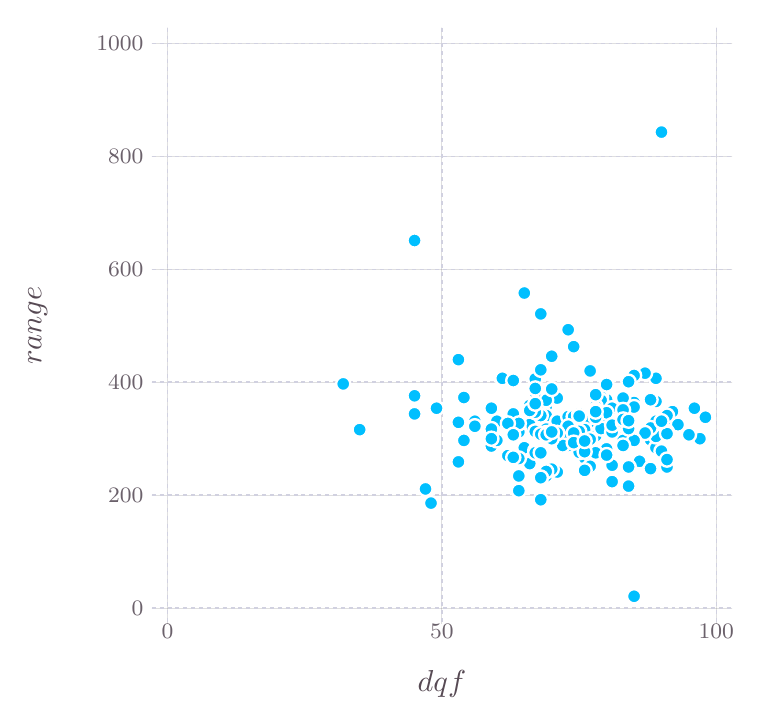
\begin{tikzpicture}[x=1mm,y=-1mm]
\definecolor{mycolor000000}{rgb}{0,0,0}
\definecolor{mycolorFFFFFF}{rgb}{1,1,1}
\definecolor{mycolor564A55}{rgb}{0.34,0.29,0.33}
\definecolor{mycolorD0D0E0}{rgb}{0.82,0.82,0.88}
\definecolor{mycolor000000}{rgb}{0,0,0}
\definecolor{mycolor6C606B}{rgb}{0.42,0.38,0.42}
\definecolor{mycolor00BFFF}{rgb}{0,0.75,1}
\begin{scope}
\begin{scope}
\draw (58.15,88.39) node [text=mycolor564A55,draw=mycolor000000,draw opacity=0,rotate around={-0: (0,1.81)},inner sep=0.0]{\fontsize{3.88mm}{4.66mm}\selectfont $\text{dqf}$};
\end{scope}
\begin{scope}
\draw (23.31,81.72) node [text=mycolor6C606B,rotate around={-0: (34.85,1.34)},inner sep=0.0]{\fontsize{2.82mm}{3.39mm}\selectfont $\text{0}$};
\draw (58.15,81.72) node [text=mycolor6C606B,rotate around={-0: (0,1.34)},inner sep=0.0]{\fontsize{2.82mm}{3.39mm}\selectfont $\text{50}$};
\draw (93,81.72) node [text=mycolor6C606B,rotate around={-0: (-34.85,1.34)},inner sep=0.0]{\fontsize{2.82mm}{3.39mm}\selectfont $\text{100}$};
\end{scope}
\begin{scope}
\clip  (21.31,5) -- (95,5) -- (95,80.72) -- (21.31,80.72);
\begin{scope}
\clip  (21.31,5) -- (95,5) -- (95,80.72) -- (21.31,80.72);
\path [fill=mycolor000000,fill opacity=0,draw=mycolor000000,draw opacity=0] (21.31,5) rectangle +(73.69,75.72);
\end{scope}
\begin{scope}
[dash pattern=on 0.5mm off 0.5mm,line width=0.2mm]
\path [fill=mycolor000000,draw=mycolorD0D0E0]  (21.31,78.72) -- (95,78.72);
\path [fill=mycolor000000,draw=mycolorD0D0E0]  (21.31,64.37) -- (95,64.37);
\path [fill=mycolor000000,draw=mycolorD0D0E0]  (21.31,50.03) -- (95,50.03);
\path [fill=mycolor000000,draw=mycolorD0D0E0]  (21.31,35.69) -- (95,35.69);
\path [fill=mycolor000000,draw=mycolorD0D0E0]  (21.31,21.34) -- (95,21.34);
\path [fill=mycolor000000,draw=mycolorD0D0E0]  (21.31,7) -- (95,7);
\end{scope}
\begin{scope}
[dash pattern=on 0.5mm off 0.5mm,line width=0.2mm]
\path [fill=mycolor000000,draw=mycolorD0D0E0]  (23.31,5) -- (23.31,80.72);
\path [fill=mycolor000000,draw=mycolorD0D0E0]  (58.15,5) -- (58.15,80.72);
\path [fill=mycolor000000,draw=mycolorD0D0E0]  (93,5) -- (93,80.72);
\end{scope}
\begin{scope}
\begin{scope}
\begin{scope}
[line width=0.3mm]
\path [fill=mycolor00BFFF,draw=mycolorFFFFFF] (82.55,77.21) circle [radius=0.9];
\path [fill=mycolor00BFFF,draw=mycolorFFFFFF] (84.64,57.34) circle [radius=0.9];
\path [fill=mycolor00BFFF,draw=mycolorFFFFFF] (56.06,63.58) circle [radius=0.9];
\path [fill=mycolor00BFFF,draw=mycolorFFFFFF] (87.42,54.98) circle [radius=0.9];
\path [fill=mycolor00BFFF,draw=mycolorFFFFFF] (85.33,49.53) circle [radius=0.9];
\path [fill=mycolor00BFFF,draw=mycolorFFFFFF] (77.67,54.55) circle [radius=0.9];
\path [fill=mycolor00BFFF,draw=mycolorFFFFFF] (65.82,49.53) circle [radius=0.9];
\path [fill=mycolor00BFFF,draw=mycolorFFFFFF] (68.61,38.7) circle [radius=0.9];
\path [fill=mycolor00BFFF,draw=mycolorFFFFFF] (70.7,64.95) circle [radius=0.9];
\path [fill=mycolor00BFFF,draw=mycolorFFFFFF] (72.79,61.43) circle [radius=0.9];
\path [fill=mycolor00BFFF,draw=mycolorFFFFFF] (83.24,60.07) circle [radius=0.9];
\path [fill=mycolor00BFFF,draw=mycolorFFFFFF] (79.76,62.65) circle [radius=0.9];
\path [fill=mycolor00BFFF,draw=mycolorFFFFFF] (90.91,57.2) circle [radius=0.9];
\path [fill=mycolor00BFFF,draw=mycolorFFFFFF] (64.43,58.13) circle [radius=0.9];
\path [fill=mycolor00BFFF,draw=mycolorFFFFFF] (83.94,48.88) circle [radius=0.9];
\path [fill=mycolor00BFFF,draw=mycolorFFFFFF] (76.27,59.64) circle [radius=0.9];
\path [fill=mycolor00BFFF,draw=mycolorFFFFFF] (85.33,58.35) circle [radius=0.9];
\path [fill=mycolor00BFFF,draw=mycolorFFFFFF] (47.7,56.05) circle [radius=0.9];
\path [fill=mycolor00BFFF,draw=mycolorFFFFFF] (80.45,55.77) circle [radius=0.9];
\path [fill=mycolor00BFFF,draw=mycolorFFFFFF] (69.3,55.41) circle [radius=0.9];
\path [fill=mycolor00BFFF,draw=mycolorFFFFFF] (75.58,56.77) circle [radius=0.9];
\path [fill=mycolor00BFFF,draw=mycolorFFFFFF] (74.88,45.51) circle [radius=0.9];
\path [fill=mycolor00BFFF,draw=mycolorFFFFFF] (67.91,56.05) circle [radius=0.9];
\path [fill=mycolor00BFFF,draw=mycolorFFFFFF] (65.12,54.98) circle [radius=0.9];
\path [fill=mycolor00BFFF,draw=mycolorFFFFFF] (86.03,18.26) circle [radius=0.9];
\path [fill=mycolor00BFFF,draw=mycolorFFFFFF] (60.94,57.42) circle [radius=0.9];
\path [fill=mycolor00BFFF,draw=mycolorFFFFFF] (68.61,58.35) circle [radius=0.9];
\path [fill=mycolor00BFFF,draw=mycolorFFFFFF] (79.06,52.25) circle [radius=0.9];
\path [fill=mycolor00BFFF,draw=mycolorFFFFFF] (72.79,52.04) circle [radius=0.9];
\path [fill=mycolor00BFFF,draw=mycolorFFFFFF] (69.3,60.36) circle [radius=0.9];
\path [fill=mycolor00BFFF,draw=mycolorFFFFFF] (76.97,60.71) circle [radius=0.9];
\path [fill=mycolor00BFFF,draw=mycolorFFFFFF] (87.42,53.76) circle [radius=0.9];
\path [fill=mycolor00BFFF,draw=mycolorFFFFFF] (71.39,53.11) circle [radius=0.9];
\path [fill=mycolor00BFFF,draw=mycolorFFFFFF] (82.55,49.17) circle [radius=0.9];
\path [fill=mycolor00BFFF,draw=mycolorFFFFFF] (72.09,55.62) circle [radius=0.9];
\path [fill=mycolor00BFFF,draw=mycolorFFFFFF] (76.97,55.12) circle [radius=0.9];
\path [fill=mycolor00BFFF,draw=mycolorFFFFFF] (75.58,55.12) circle [radius=0.9];
\path [fill=mycolor00BFFF,draw=mycolorFFFFFF] (75.58,55.98) circle [radius=0.9];
\path [fill=mycolor00BFFF,draw=mycolorFFFFFF] (79.06,53.97) circle [radius=0.9];
\path [fill=mycolor00BFFF,draw=mycolorFFFFFF] (85.33,54.98) circle [radius=0.9];
\path [fill=mycolor00BFFF,draw=mycolorFFFFFF] (76.97,55.05) circle [radius=0.9];
\path [fill=mycolor00BFFF,draw=mycolorFFFFFF] (74.18,54.12) circle [radius=0.9];
\path [fill=mycolor00BFFF,draw=mycolorFFFFFF] (64.43,55.98) circle [radius=0.9];
\path [fill=mycolor00BFFF,draw=mycolorFFFFFF] (71.39,54.26) circle [radius=0.9];
\path [fill=mycolor00BFFF,draw=mycolorFFFFFF] (67.91,61.93) circle [radius=0.9];
\path [fill=mycolor00BFFF,draw=mycolorFFFFFF] (74.18,54.26) circle [radius=0.9];
\path [fill=mycolor00BFFF,draw=mycolorFFFFFF] (65.12,57.42) circle [radius=0.9];
\path [fill=mycolor00BFFF,draw=mycolorFFFFFF] (67.91,56.34) circle [radius=0.9];
\path [fill=mycolor00BFFF,draw=mycolorFFFFFF] (74.18,56.99) circle [radius=0.9];
\path [fill=mycolor00BFFF,draw=mycolorFFFFFF] (54.67,54.05) circle [radius=0.9];
\path [fill=mycolor00BFFF,draw=mycolorFFFFFF] (69.3,52.97) circle [radius=0.9];
\path [fill=mycolor00BFFF,draw=mycolorFFFFFF] (81.15,53.97) circle [radius=0.9];
\path [fill=mycolor00BFFF,draw=mycolorFFFFFF] (74.18,57.13) circle [radius=0.9];
\path [fill=mycolor00BFFF,draw=mycolorFFFFFF] (72.09,46.73) circle [radius=0.9];
\path [fill=mycolor00BFFF,draw=mycolorFFFFFF] (91.61,54.48) circle [radius=0.9];
\path [fill=mycolor00BFFF,draw=mycolorFFFFFF] (77.67,56.84) circle [radius=0.9];
\path [fill=mycolor00BFFF,draw=mycolorFFFFFF] (71.39,55.98) circle [radius=0.9];
\path [fill=mycolor00BFFF,draw=mycolorFFFFFF] (71.39,52.32) circle [radius=0.9];
\path [fill=mycolor00BFFF,draw=mycolorFFFFFF] (70.7,54.26) circle [radius=0.9];
\path [fill=mycolor00BFFF,draw=mycolorFFFFFF] (78.36,51.89) circle [radius=0.9];
\path [fill=mycolor00BFFF,draw=mycolorFFFFFF] (85.33,52.47) circle [radius=0.9];
\path [fill=mycolor00BFFF,draw=mycolorFFFFFF] (78.36,52.32) circle [radius=0.9];
\path [fill=mycolor00BFFF,draw=mycolorFFFFFF] (86.73,56.48) circle [radius=0.9];
\path [fill=mycolor00BFFF,draw=mycolorFFFFFF] (77.67,53.11) circle [radius=0.9];
\path [fill=mycolor00BFFF,draw=mycolorFFFFFF] (74.88,56.27) circle [radius=0.9];
\path [fill=mycolor00BFFF,draw=mycolorFFFFFF] (76.27,54.98) circle [radius=0.9];
\path [fill=mycolor00BFFF,draw=mycolorFFFFFF] (74.88,54.48) circle [radius=0.9];
\path [fill=mycolor00BFFF,draw=mycolorFFFFFF] (79.06,58.49) circle [radius=0.9];
\path [fill=mycolor00BFFF,draw=mycolorFFFFFF] (82.55,52.61) circle [radius=0.9];
\path [fill=mycolor00BFFF,draw=mycolorFFFFFF] (81.85,54.12) circle [radius=0.9];
\path [fill=mycolor00BFFF,draw=mycolorFFFFFF] (78.36,54.33) circle [radius=0.9];
\path [fill=mycolor00BFFF,draw=mycolorFFFFFF] (77.67,53.54) circle [radius=0.9];
\path [fill=mycolor00BFFF,draw=mycolorFFFFFF] (81.15,57.42) circle [radius=0.9];
\path [fill=mycolor00BFFF,draw=mycolorFFFFFF] (88.12,55.41) circle [radius=0.9];
\path [fill=mycolor00BFFF,draw=mycolorFFFFFF] (90.21,53.33) circle [radius=0.9];
\path [fill=mycolor00BFFF,draw=mycolorFFFFFF] (74.88,54.26) circle [radius=0.9];
\path [fill=mycolor00BFFF,draw=mycolorFFFFFF] (78.36,55.91) circle [radius=0.9];
\path [fill=mycolor00BFFF,draw=mycolorFFFFFF] (77.67,51.61) circle [radius=0.9];
\path [fill=mycolor00BFFF,draw=mycolorFFFFFF] (84.64,52.25) circle [radius=0.9];
\path [fill=mycolor00BFFF,draw=mycolorFFFFFF] (79.76,53.33) circle [radius=0.9];
\path [fill=mycolor00BFFF,draw=mycolorFFFFFF] (79.06,53.9) circle [radius=0.9];
\path [fill=mycolor00BFFF,draw=mycolorFFFFFF] (77.67,54.48) circle [radius=0.9];
\path [fill=mycolor00BFFF,draw=mycolorFFFFFF] (85.33,56.91) circle [radius=0.9];
\path [fill=mycolor00BFFF,draw=mycolorFFFFFF] (81.15,52.04) circle [radius=0.9];
\path [fill=mycolor00BFFF,draw=mycolorFFFFFF] (81.85,49.96) circle [radius=0.9];
\path [fill=mycolor00BFFF,draw=mycolorFFFFFF] (70,51.32) circle [radius=0.9];
\path [fill=mycolor00BFFF,draw=mycolorFFFFFF] (67.21,54.05) circle [radius=0.9];
\path [fill=mycolor00BFFF,draw=mycolorFFFFFF] (70,49.6) circle [radius=0.9];
\path [fill=mycolor00BFFF,draw=mycolorFFFFFF] (72.79,54.98) circle [radius=0.9];
\path [fill=mycolor00BFFF,draw=mycolorFFFFFF] (77.67,53.76) circle [radius=0.9];
\path [fill=mycolor00BFFF,draw=mycolorFFFFFF] (81.15,53.97) circle [radius=0.9];
\path [fill=mycolor00BFFF,draw=mycolorFFFFFF] (74.18,54.4) circle [radius=0.9];
\path [fill=mycolor00BFFF,draw=mycolorFFFFFF] (75.58,54.26) circle [radius=0.9];
\path [fill=mycolor00BFFF,draw=mycolorFFFFFF] (91.61,54.48) circle [radius=0.9];
\path [fill=mycolor00BFFF,draw=mycolorFFFFFF] (79.06,50.32) circle [radius=0.9];
\path [fill=mycolor00BFFF,draw=mycolorFFFFFF] (76.27,56.05) circle [radius=0.9];
\path [fill=mycolor00BFFF,draw=mycolorFFFFFF] (81.85,54.76) circle [radius=0.9];
\path [fill=mycolor00BFFF,draw=mycolorFFFFFF] (71.39,56.48) circle [radius=0.9];
\path [fill=mycolor00BFFF,draw=mycolorFFFFFF] (62.33,54.98) circle [radius=0.9];
\path [fill=mycolor00BFFF,draw=mycolorFFFFFF] (54.67,51.75) circle [radius=0.9];
\path [fill=mycolor00BFFF,draw=mycolorFFFFFF] (45.61,50.24) circle [radius=0.9];
\path [fill=mycolor00BFFF,draw=mycolorFFFFFF] (75.58,56.27) circle [radius=0.9];
\path [fill=mycolor00BFFF,draw=mycolorFFFFFF] (60.24,55.12) circle [radius=0.9];
\path [fill=mycolor00BFFF,draw=mycolorFFFFFF] (56.76,65.38) circle [radius=0.9];
\path [fill=mycolor00BFFF,draw=mycolorFFFFFF] (74.18,58.06) circle [radius=0.9];
\path [fill=mycolor00BFFF,draw=mycolorFFFFFF] (70.7,48.45) circle [radius=0.9];
\path [fill=mycolor00BFFF,draw=mycolorFFFFFF] (76.27,61.22) circle [radius=0.9];
\path [fill=mycolor00BFFF,draw=mycolorFFFFFF] (67.91,55.26) circle [radius=0.9];
\path [fill=mycolor00BFFF,draw=mycolorFFFFFF] (82.55,53.18) circle [radius=0.9];
\path [fill=mycolor00BFFF,draw=mycolorFFFFFF] (60.94,51.97) circle [radius=0.9];
\path [fill=mycolor00BFFF,draw=mycolorFFFFFF] (77.67,58.99) circle [radius=0.9];
\path [fill=mycolor00BFFF,draw=mycolorFFFFFF] (75.58,58.92) circle [radius=0.9];
\path [fill=mycolor00BFFF,draw=mycolorFFFFFF] (72.09,50.89) circle [radius=0.9];
\path [fill=mycolor00BFFF,draw=mycolorFFFFFF] (70.7,41.35) circle [radius=0.9];
\path [fill=mycolor00BFFF,draw=mycolorFFFFFF] (70.7,41.35) circle [radius=0.9];
\path [fill=mycolor00BFFF,draw=mycolorFFFFFF] (86.73,56.34) circle [radius=0.9];
\path [fill=mycolor00BFFF,draw=mycolorFFFFFF] (70,53.83) circle [radius=0.9];
\path [fill=mycolor00BFFF,draw=mycolorFFFFFF] (86.73,54.26) circle [radius=0.9];
\path [fill=mycolor00BFFF,draw=mycolorFFFFFF] (74.18,43.36) circle [radius=0.9];
\path [fill=mycolor00BFFF,draw=mycolorFFFFFF] (86.73,60.79) circle [radius=0.9];
\path [fill=mycolor00BFFF,draw=mycolorFFFFFF] (84.64,61) circle [radius=0.9];
\path [fill=mycolor00BFFF,draw=mycolorFFFFFF] (84.64,55.84) circle [radius=0.9];
\path [fill=mycolor00BFFF,draw=mycolorFFFFFF] (66.52,59.42) circle [radius=0.9];
\path [fill=mycolor00BFFF,draw=mycolorFFFFFF] (74.88,54.4) circle [radius=0.9];
\path [fill=mycolor00BFFF,draw=mycolorFFFFFF] (73.49,58.06) circle [radius=0.9];
\path [fill=mycolor00BFFF,draw=mycolorFFFFFF] (86.73,56.56) circle [radius=0.9];
\path [fill=mycolor00BFFF,draw=mycolorFFFFFF] (74.18,55.62) circle [radius=0.9];
\path [fill=mycolor00BFFF,draw=mycolorFFFFFF] (76.27,58.85) circle [radius=0.9];
\path [fill=mycolor00BFFF,draw=mycolorFFFFFF] (76.97,48.59) circle [radius=0.9];
\path [fill=mycolor00BFFF,draw=mycolorFFFFFF] (69.3,53.61) circle [radius=0.9];
\path [fill=mycolor00BFFF,draw=mycolorFFFFFF] (71.39,61.93) circle [radius=0.9];
\path [fill=mycolor00BFFF,draw=mycolorFFFFFF] (74.88,56.48) circle [radius=0.9];
\path [fill=mycolor00BFFF,draw=mycolorFFFFFF] (70,56.27) circle [radius=0.9];
\path [fill=mycolor00BFFF,draw=mycolorFFFFFF] (86.03,54.98) circle [radius=0.9];
\path [fill=mycolor00BFFF,draw=mycolorFFFFFF] (83.94,56.48) circle [radius=0.9];
\path [fill=mycolor00BFFF,draw=mycolorFFFFFF] (76.97,57.27) circle [radius=0.9];
\path [fill=mycolor00BFFF,draw=mycolorFFFFFF] (82.55,57.42) circle [radius=0.9];
\path [fill=mycolor00BFFF,draw=mycolorFFFFFF] (81.15,55.41) circle [radius=0.9];
\path [fill=mycolor00BFFF,draw=mycolorFFFFFF] (81.15,58.06) circle [radius=0.9];
\path [fill=mycolor00BFFF,draw=mycolorFFFFFF] (67.91,59.71) circle [radius=0.9];
\path [fill=mycolor00BFFF,draw=mycolorFFFFFF] (66.52,59.35) circle [radius=0.9];
\path [fill=mycolor00BFFF,draw=mycolorFFFFFF] (79.76,60.57) circle [radius=0.9];
\path [fill=mycolor00BFFF,draw=mycolorFFFFFF] (74.88,57.7) circle [radius=0.9];
\path [fill=mycolor00BFFF,draw=mycolorFFFFFF] (81.15,53.54) circle [radius=0.9];
\path [fill=mycolor00BFFF,draw=mycolorFFFFFF] (70.7,56.63) circle [radius=0.9];
\path [fill=mycolor00BFFF,draw=mycolorFFFFFF] (79.76,56.34) circle [radius=0.9];
\path [fill=mycolor00BFFF,draw=mycolorFFFFFF] (60.24,60.14) circle [radius=0.9];
\path [fill=mycolor00BFFF,draw=mycolorFFFFFF] (72.09,61.07) circle [radius=0.9];
\path [fill=mycolor00BFFF,draw=mycolorFFFFFF] (72.79,56.48) circle [radius=0.9];
\path [fill=mycolor00BFFF,draw=mycolorFFFFFF] (72.79,56.48) circle [radius=0.9];
\path [fill=mycolor00BFFF,draw=mycolorFFFFFF] (72.09,56.48) circle [radius=0.9];
\path [fill=mycolor00BFFF,draw=mycolorFFFFFF] (72.09,57.2) circle [radius=0.9];
\path [fill=mycolor00BFFF,draw=mycolorFFFFFF] (70,58.71) circle [radius=0.9];
\path [fill=mycolor00BFFF,draw=mycolorFFFFFF] (66.52,55.26) circle [radius=0.9];
\path [fill=mycolor00BFFF,draw=mycolorFFFFFF] (70,52.75) circle [radius=0.9];
\path [fill=mycolor00BFFF,draw=mycolorFFFFFF] (75.58,54.05) circle [radius=0.9];
\path [fill=mycolor00BFFF,draw=mycolorFFFFFF] (71.39,56.7) circle [radius=0.9];
\path [fill=mycolor00BFFF,draw=mycolorFFFFFF] (64.43,57.2) circle [radius=0.9];
\path [fill=mycolor00BFFF,draw=mycolorFFFFFF] (79.76,55.48) circle [radius=0.9];
\path [fill=mycolor00BFFF,draw=mycolorFFFFFF] (86.03,58.78) circle [radius=0.9];
\path [fill=mycolor00BFFF,draw=mycolorFFFFFF] (70,58.99) circle [radius=0.9];
\path [fill=mycolor00BFFF,draw=mycolorFFFFFF] (81.15,55.12) circle [radius=0.9];
\path [fill=mycolor00BFFF,draw=mycolorFFFFFF] (81.15,55.12) circle [radius=0.9];
\path [fill=mycolor00BFFF,draw=mycolorFFFFFF] (71.39,61.36) circle [radius=0.9];
\path [fill=mycolor00BFFF,draw=mycolorFFFFFF] (89.52,56.7) circle [radius=0.9];
\path [fill=mycolor00BFFF,draw=mycolorFFFFFF] (81.85,55.91) circle [radius=0.9];
\path [fill=mycolor00BFFF,draw=mycolorFFFFFF] (67.21,49.81) circle [radius=0.9];
\path [fill=mycolor00BFFF,draw=mycolorFFFFFF] (67.21,59.57) circle [radius=0.9];
\path [fill=mycolor00BFFF,draw=mycolorFFFFFF] (81.15,54.76) circle [radius=0.9];
\path [fill=mycolor00BFFF,draw=mycolorFFFFFF] (70.7,62.15) circle [radius=0.9];
\path [fill=mycolor00BFFF,draw=mycolorFFFFFF] (70.7,62.15) circle [radius=0.9];
\path [fill=mycolor00BFFF,draw=mycolorFFFFFF] (67.91,63.8) circle [radius=0.9];
\path [fill=mycolor00BFFF,draw=mycolorFFFFFF] (79.06,59.28) circle [radius=0.9];
\path [fill=mycolor00BFFF,draw=mycolorFFFFFF] (67.21,56.7) circle [radius=0.9];
\path [fill=mycolor00BFFF,draw=mycolorFFFFFF] (81.85,60.79) circle [radius=0.9];
\path [fill=mycolor00BFFF,draw=mycolorFFFFFF] (81.85,60.79) circle [radius=0.9];
\path [fill=mycolor00BFFF,draw=mycolorFFFFFF] (64.43,53.33) circle [radius=0.9];
\path [fill=mycolor00BFFF,draw=mycolorFFFFFF] (76.27,57.49) circle [radius=0.9];
\path [fill=mycolor00BFFF,draw=mycolorFFFFFF] (70,50.82) circle [radius=0.9];
\path [fill=mycolor00BFFF,draw=mycolorFFFFFF] (70.7,58.99) circle [radius=0.9];
\path [fill=mycolor00BFFF,draw=mycolorFFFFFF] (57.46,53.33) circle [radius=0.9];
\path [fill=mycolor00BFFF,draw=mycolorFFFFFF] (86.73,59.85) circle [radius=0.9];
\path [fill=mycolor00BFFF,draw=mycolorFFFFFF] (81.85,63.22) circle [radius=0.9];
\path [fill=mycolor00BFFF,draw=mycolorFFFFFF] (60.24,47.16) circle [radius=0.9];
\path [fill=mycolor00BFFF,draw=mycolorFFFFFF] (72.09,56.34) circle [radius=0.9];
\path [fill=mycolor00BFFF,draw=mycolorFFFFFF] (81.85,54.91) circle [radius=0.9];
\path [fill=mycolor00BFFF,draw=mycolorFFFFFF] (62.33,55.62) circle [radius=0.9];
\path [fill=mycolor00BFFF,draw=mycolorFFFFFF] (54.67,32.03) circle [radius=0.9];
\path [fill=mycolor00BFFF,draw=mycolorFFFFFF] (75.58,54.33) circle [radius=0.9];
\end{scope}
\end{scope}
\end{scope}
\end{scope}
\begin{scope}
\draw (20.31,78.72) node [text=mycolor6C606B,rotate around={-0: (-3.35,-35.86)},left,inner sep=0.0]{\fontsize{2.82mm}{3.39mm}\selectfont $\text{0}$};
\draw (20.31,64.37) node [text=mycolor6C606B,rotate around={-0: (-3.35,-21.51)},left,inner sep=0.0]{\fontsize{2.82mm}{3.39mm}\selectfont $\text{200}$};
\draw (20.31,50.03) node [text=mycolor6C606B,rotate around={-0: (-3.35,-7.17)},left,inner sep=0.0]{\fontsize{2.82mm}{3.39mm}\selectfont $\text{400}$};
\draw (20.31,35.69) node [text=mycolor6C606B,rotate around={-0: (-3.35,7.17)},left,inner sep=0.0]{\fontsize{2.82mm}{3.39mm}\selectfont $\text{600}$};
\draw (20.31,21.34) node [text=mycolor6C606B,rotate around={-0: (-3.35,21.51)},left,inner sep=0.0]{\fontsize{2.82mm}{3.39mm}\selectfont $\text{800}$};
\draw (20.31,7) node [text=mycolor6C606B,rotate around={-0: (-3.35,35.86)},left,inner sep=0.0]{\fontsize{2.82mm}{3.39mm}\selectfont $\text{1000}$};
\end{scope}
\begin{scope}
\draw (8.81,40.86) node [text=mycolor564A55,draw=mycolor000000,draw opacity=0,rotate around={90: (0,2)},inner sep=0.0]{\fontsize{3.88mm}{4.66mm}\selectfont $\text{range}$};
\end{scope}
\end{scope}
\end{tikzpicture}

%	\caption{100 values measured at \SI{2}{\metre} distance}
%	\label{2m}
%\end{figure}
\begin{figure}[h]
	\centering
	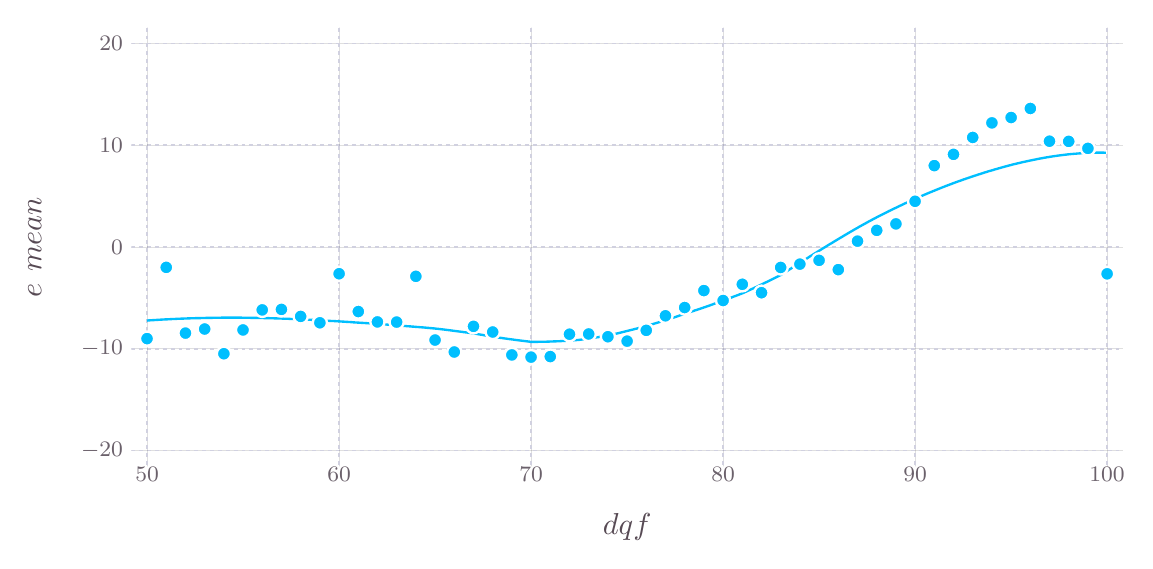
\begin{tikzpicture}[x=1mm,y=-1mm]
\definecolor{mycolor000000}{rgb}{0,0,0}
\definecolor{mycolorD0D0E0}{rgb}{0.82,0.82,0.88}
\definecolor{mycolor564A55}{rgb}{0.34,0.29,0.33}
\definecolor{mycolor6C606B}{rgb}{0.42,0.38,0.42}
\definecolor{mycolor00BFFF}{rgb}{0,0.75,1}
\definecolor{mycolor000000}{rgb}{0,0,0}
\definecolor{mycolorFFFFFF}{rgb}{1,1,1}
\begin{scope}
\begin{scope}
\draw (82.04,68.39) node [text=mycolor564A55,draw=mycolor000000,draw opacity=0,rotate around={-0: (0,1.81)},inner sep=0.0]{\fontsize{3.88mm}{4.66mm}\selectfont $\text{dqf}$};
\end{scope}
\begin{scope}
\draw (21.07,61.72) node [text=mycolor6C606B,rotate around={-0: (60.96,1.34)},inner sep=0.0]{\fontsize{2.82mm}{3.39mm}\selectfont $\text{50}$};
\draw (45.46,61.72) node [text=mycolor6C606B,rotate around={-0: (36.58,1.34)},inner sep=0.0]{\fontsize{2.82mm}{3.39mm}\selectfont $\text{60}$};
\draw (69.84,61.72) node [text=mycolor6C606B,rotate around={-0: (12.19,1.34)},inner sep=0.0]{\fontsize{2.82mm}{3.39mm}\selectfont $\text{70}$};
\draw (94.23,61.72) node [text=mycolor6C606B,rotate around={-0: (-12.19,1.34)},inner sep=0.0]{\fontsize{2.82mm}{3.39mm}\selectfont $\text{80}$};
\draw (118.61,61.72) node [text=mycolor6C606B,rotate around={-0: (-36.58,1.34)},inner sep=0.0]{\fontsize{2.82mm}{3.39mm}\selectfont $\text{90}$};
\draw (143,61.72) node [text=mycolor6C606B,rotate around={-0: (-60.96,1.34)},inner sep=0.0]{\fontsize{2.82mm}{3.39mm}\selectfont $\text{100}$};
\end{scope}
\begin{scope}
\clip  (19.07,5) -- (145,5) -- (145,60.72) -- (19.07,60.72);
\begin{scope}
\clip  (19.07,5) -- (145,5) -- (145,60.72) -- (19.07,60.72);
\path [fill=mycolor000000,fill opacity=0,draw=mycolor000000,draw opacity=0] (19.07,5) rectangle +(125.93,55.72);
\end{scope}
\begin{scope}
[dash pattern=on 0.5mm off 0.5mm,line width=0.2mm]
\path [fill=mycolor000000,draw=mycolorD0D0E0]  (19.07,58.72) -- (145,58.72);
\path [fill=mycolor000000,draw=mycolorD0D0E0]  (19.07,45.79) -- (145,45.79);
\path [fill=mycolor000000,draw=mycolorD0D0E0]  (19.07,32.86) -- (145,32.86);
\path [fill=mycolor000000,draw=mycolorD0D0E0]  (19.07,19.93) -- (145,19.93);
\path [fill=mycolor000000,draw=mycolorD0D0E0]  (19.07,7) -- (145,7);
\end{scope}
\begin{scope}
[dash pattern=on 0.5mm off 0.5mm,line width=0.2mm]
\path [fill=mycolor000000,draw=mycolorD0D0E0]  (21.07,5) -- (21.07,60.72);
\path [fill=mycolor000000,draw=mycolorD0D0E0]  (45.46,5) -- (45.46,60.72);
\path [fill=mycolor000000,draw=mycolorD0D0E0]  (69.84,5) -- (69.84,60.72);
\path [fill=mycolor000000,draw=mycolorD0D0E0]  (94.23,5) -- (94.23,60.72);
\path [fill=mycolor000000,draw=mycolorD0D0E0]  (118.61,5) -- (118.61,60.72);
\path [fill=mycolor000000,draw=mycolorD0D0E0]  (143,5) -- (143,60.72);
\end{scope}
\begin{scope}
\begin{scope}
[line width=0.3mm]
\path [fill=mycolor000000,fill opacity=0,draw=mycolor00BFFF]  (21.07,42.2) -- (21.24,42.18) -- (21.4,42.17) -- (21.56,42.16) -- (21.72,42.15) -- (21.89,42.14) -- (22.05,42.13) -- (22.21,42.12) -- (22.37,42.11) -- (22.54,42.1) -- (22.7,42.09) -- (22.86,42.08) -- (23.02,42.07) -- (23.19,42.06) -- (23.35,42.05) -- (23.51,42.04) -- (23.67,42.04) -- (23.84,42.03) -- (24,42.02) -- (24.16,42.01) -- (24.32,42) -- (24.49,42) -- (24.65,41.99) -- (24.81,41.98) -- (24.97,41.97) -- (25.14,41.97) -- (25.3,41.96) -- (25.46,41.95) -- (25.62,41.95) -- (25.79,41.94) -- (25.95,41.94) -- (26.11,41.93) -- (26.28,41.92) -- (26.44,41.92) -- (26.6,41.91) -- (26.76,41.91) -- (26.93,41.9) -- (27.09,41.9) -- (27.25,41.89) -- (27.41,41.89) -- (27.58,41.88) -- (27.74,41.88) -- (27.9,41.88) -- (28.06,41.87) -- (28.23,41.87) -- (28.39,41.87) -- (28.55,41.86) -- (28.71,41.86) -- (28.88,41.86) -- (29.04,41.85) -- (29.2,41.85) -- (29.36,41.85) -- (29.53,41.84) -- (29.69,41.84) -- (29.85,41.84) -- (30.01,41.84) -- (30.18,41.84) -- (30.34,41.84) -- (30.5,41.83) -- (30.66,41.83) -- (30.83,41.83) -- (30.99,41.83) -- (31.15,41.83) -- (31.31,41.83) -- (31.48,41.83) -- (31.64,41.83) -- (31.8,41.83) -- (31.97,41.83) -- (32.13,41.83) -- (32.29,41.83) -- (32.45,41.83) -- (32.62,41.83) -- (32.78,41.83) -- (32.94,41.83) -- (33.1,41.83) -- (33.27,41.84) -- (33.43,41.84) -- (33.59,41.84) -- (33.75,41.84) -- (33.92,41.84) -- (34.08,41.84) -- (34.24,41.85) -- (34.4,41.85) -- (34.57,41.85) -- (34.73,41.85) -- (34.89,41.86) -- (35.05,41.86) -- (35.22,41.86) -- (35.38,41.87) -- (35.54,41.87) -- (35.7,41.87) -- (35.87,41.88) -- (36.03,41.88) -- (36.19,41.89) -- (36.35,41.89) -- (36.52,41.89) -- (36.68,41.9) -- (36.84,41.9) -- (37,41.91) -- (37.17,41.91) -- (37.33,41.92) -- (37.49,41.92) -- (37.66,41.93) -- (37.82,41.93) -- (37.98,41.94) -- (38.14,41.94) -- (38.31,41.95) -- (38.47,41.96) -- (38.63,41.96) -- (38.79,41.97) -- (38.96,41.97) -- (39.12,41.98) -- (39.28,41.99) -- (39.44,41.99) -- (39.61,42) -- (39.77,42.01) -- (39.93,42.01) -- (40.09,42.02) -- (40.26,42.03) -- (40.42,42.04) -- (40.58,42.04) -- (40.74,42.05) -- (40.91,42.06) -- (41.07,42.07) -- (41.23,42.07) -- (41.39,42.08) -- (41.56,42.09) -- (41.72,42.1) -- (41.88,42.1) -- (42.04,42.11) -- (42.21,42.12) -- (42.37,42.13) -- (42.53,42.14) -- (42.69,42.15) -- (42.86,42.16) -- (43.02,42.16) -- (43.18,42.17) -- (43.35,42.18) -- (43.51,42.19) -- (43.67,42.2) -- (43.83,42.21) -- (44,42.22) -- (44.16,42.23) -- (44.32,42.24) -- (44.48,42.25) -- (44.65,42.25) -- (44.81,42.26) -- (44.97,42.27) -- (45.13,42.28) -- (45.3,42.29) -- (45.46,42.3) -- (45.62,42.31) -- (45.78,42.32) -- (45.95,42.33) -- (46.11,42.34) -- (46.27,42.35) -- (46.43,42.36) -- (46.6,42.37) -- (46.76,42.38) -- (46.92,42.39) -- (47.08,42.4) -- (47.25,42.42) -- (47.41,42.43) -- (47.57,42.44) -- (47.73,42.45) -- (47.9,42.46) -- (48.06,42.47) -- (48.22,42.48) -- (48.38,42.49) -- (48.55,42.5) -- (48.71,42.51) -- (48.87,42.52) -- (49.04,42.53) -- (49.2,42.54) -- (49.36,42.56) -- (49.52,42.57) -- (49.69,42.58) -- (49.85,42.59) -- (50.01,42.6) -- (50.17,42.61) -- (50.34,42.62) -- (50.5,42.63) -- (50.66,42.65) -- (50.82,42.66) -- (50.99,42.67) -- (51.15,42.68) -- (51.31,42.69) -- (51.47,42.7) -- (51.64,42.72) -- (51.8,42.73) -- (51.96,42.74) -- (52.12,42.75) -- (52.29,42.77) -- (52.45,42.78) -- (52.61,42.79) -- (52.77,42.8) -- (52.94,42.82) -- (53.1,42.83) -- (53.26,42.84) -- (53.42,42.85) -- (53.59,42.87) -- (53.75,42.88) -- (53.91,42.89) -- (54.07,42.91) -- (54.24,42.92) -- (54.4,42.93) -- (54.56,42.94) -- (54.73,42.96) -- (54.89,42.97) -- (55.05,42.98) -- (55.21,43) -- (55.38,43.01) -- (55.54,43.02) -- (55.7,43.04) -- (55.86,43.05) -- (56.03,43.06) -- (56.19,43.07) -- (56.35,43.09) -- (56.51,43.1) -- (56.68,43.12) -- (56.84,43.13) -- (57,43.15) -- (57.16,43.16) -- (57.33,43.18) -- (57.49,43.19) -- (57.65,43.21) -- (57.81,43.23) -- (57.98,43.24) -- (58.14,43.26) -- (58.3,43.28) -- (58.46,43.3) -- (58.63,43.32) -- (58.79,43.34) -- (58.95,43.36) -- (59.11,43.38) -- (59.28,43.4) -- (59.44,43.42) -- (59.6,43.44) -- (59.76,43.46) -- (59.93,43.49) -- (60.09,43.51) -- (60.25,43.53) -- (60.42,43.55) -- (60.58,43.57) -- (60.74,43.59) -- (60.9,43.61) -- (61.07,43.63) -- (61.23,43.66) -- (61.39,43.68) -- (61.55,43.7) -- (61.72,43.72) -- (61.88,43.74) -- (62.04,43.76) -- (62.2,43.78) -- (62.37,43.8) -- (62.53,43.83) -- (62.69,43.85) -- (62.85,43.88) -- (63.02,43.91) -- (63.18,43.94) -- (63.34,43.97) -- (63.5,43.99) -- (63.67,44.02) -- (63.83,44.05) -- (63.99,44.08) -- (64.15,44.11) -- (64.32,44.14) -- (64.48,44.17) -- (64.64,44.2) -- (64.8,44.23) -- (64.97,44.25) -- (65.13,44.28) -- (65.29,44.3) -- (65.45,44.32) -- (65.62,44.34) -- (65.78,44.37) -- (65.94,44.39) -- (66.11,44.41) -- (66.27,44.43) -- (66.43,44.46) -- (66.59,44.48) -- (66.76,44.5) -- (66.92,44.53) -- (67.08,44.55) -- (67.24,44.57) -- (67.41,44.59) -- (67.57,44.61) -- (67.73,44.64) -- (67.89,44.66) -- (68.06,44.68) -- (68.22,44.7) -- (68.38,44.72) -- (68.54,44.74) -- (68.71,44.76) -- (68.87,44.78) -- (69.03,44.8) -- (69.19,44.82) -- (69.36,44.84) -- (69.52,44.86) -- (69.68,44.88) -- (69.84,44.9) -- (70.01,44.9) -- (70.17,44.9) -- (70.33,44.9) -- (70.49,44.9) -- (70.66,44.9) -- (70.82,44.89) -- (70.98,44.89) -- (71.14,44.89) -- (71.31,44.89) -- (71.47,44.88) -- (71.63,44.88) -- (71.8,44.88) -- (71.96,44.87) -- (72.12,44.87) -- (72.28,44.86) -- (72.45,44.86) -- (72.61,44.85) -- (72.77,44.84) -- (72.93,44.84) -- (73.1,44.83) -- (73.26,44.82) -- (73.42,44.82) -- (73.58,44.81) -- (73.75,44.8) -- (73.91,44.79) -- (74.07,44.78) -- (74.23,44.77) -- (74.4,44.76) -- (74.56,44.75) -- (74.72,44.74) -- (74.88,44.73) -- (75.05,44.72) -- (75.21,44.71) -- (75.37,44.7) -- (75.53,44.68) -- (75.7,44.67) -- (75.86,44.66) -- (76.02,44.64) -- (76.18,44.62) -- (76.35,44.6) -- (76.51,44.58) -- (76.67,44.56) -- (76.83,44.53) -- (77,44.51) -- (77.16,44.49) -- (77.32,44.47) -- (77.49,44.44) -- (77.65,44.42) -- (77.81,44.39) -- (77.97,44.37) -- (78.14,44.34) -- (78.3,44.31) -- (78.46,44.29) -- (78.62,44.26) -- (78.79,44.23) -- (78.95,44.21) -- (79.11,44.18) -- (79.27,44.15) -- (79.44,44.12) -- (79.6,44.09) -- (79.76,44.06) -- (79.92,44.02) -- (80.09,43.98) -- (80.25,43.95) -- (80.41,43.91) -- (80.57,43.87) -- (80.74,43.84) -- (80.9,43.8) -- (81.06,43.76) -- (81.22,43.72) -- (81.39,43.68) -- (81.55,43.64) -- (81.71,43.6) -- (81.87,43.56) -- (82.04,43.52) -- (82.2,43.48) -- (82.36,43.44) -- (82.52,43.4) -- (82.69,43.36) -- (82.85,43.32) -- (83.01,43.27) -- (83.18,43.23) -- (83.34,43.19) -- (83.5,43.15) -- (83.66,43.1) -- (83.83,43.06) -- (83.99,43.02) -- (84.15,42.97) -- (84.31,42.93) -- (84.48,42.88) -- (84.64,42.83) -- (84.8,42.79) -- (84.96,42.74) -- (85.13,42.69) -- (85.29,42.65) -- (85.45,42.6) -- (85.61,42.55) -- (85.78,42.5) -- (85.94,42.45) -- (86.1,42.4) -- (86.26,42.35) -- (86.43,42.3) -- (86.59,42.25) -- (86.75,42.2) -- (86.91,42.15) -- (87.08,42.1) -- (87.24,42.05) -- (87.4,42) -- (87.56,41.95) -- (87.73,41.89) -- (87.89,41.84) -- (88.05,41.79) -- (88.21,41.73) -- (88.38,41.68) -- (88.54,41.62) -- (88.7,41.56) -- (88.87,41.5) -- (89.03,41.44) -- (89.19,41.38) -- (89.35,41.32) -- (89.52,41.27) -- (89.68,41.22) -- (89.84,41.17) -- (90,41.12) -- (90.17,41.07) -- (90.33,41.02) -- (90.49,40.97) -- (90.65,40.91) -- (90.82,40.86) -- (90.98,40.81) -- (91.14,40.75) -- (91.3,40.7) -- (91.47,40.64) -- (91.63,40.59) -- (91.79,40.53) -- (91.95,40.48) -- (92.12,40.42) -- (92.28,40.36) -- (92.44,40.31) -- (92.6,40.25) -- (92.77,40.19) -- (92.93,40.13) -- (93.09,40.07) -- (93.25,40.01) -- (93.42,39.95) -- (93.58,39.89) -- (93.74,39.83) -- (93.9,39.77) -- (94.07,39.71) -- (94.23,39.65) -- (94.39,39.59) -- (94.56,39.53) -- (94.72,39.47) -- (94.88,39.42) -- (95.04,39.36) -- (95.21,39.3) -- (95.37,39.24) -- (95.53,39.17) -- (95.69,39.11) -- (95.86,39.05) -- (96.02,38.99) -- (96.18,38.93) -- (96.34,38.86) -- (96.51,38.8) -- (96.67,38.74) -- (96.83,38.67) -- (96.99,38.59) -- (97.16,38.52) -- (97.32,38.45) -- (97.48,38.37) -- (97.64,38.3) -- (97.81,38.22) -- (97.97,38.15) -- (98.13,38.07) -- (98.29,38) -- (98.46,37.92) -- (98.62,37.84) -- (98.78,37.77) -- (98.94,37.69) -- (99.11,37.61) -- (99.27,37.54) -- (99.43,37.46) -- (99.59,37.38) -- (99.76,37.3) -- (99.92,37.22) -- (100.08,37.14) -- (100.25,37.06) -- (100.41,36.98) -- (100.57,36.9) -- (100.73,36.82) -- (100.9,36.74) -- (101.06,36.66) -- (101.22,36.58) -- (101.38,36.5) -- (101.55,36.42) -- (101.71,36.31) -- (101.87,36.21) -- (102.03,36.11) -- (102.2,36) -- (102.36,35.9) -- (102.52,35.8) -- (102.68,35.69) -- (102.85,35.59) -- (103.01,35.49) -- (103.17,35.38) -- (103.33,35.28) -- (103.5,35.18) -- (103.66,35.07) -- (103.82,34.97) -- (103.98,34.87) -- (104.15,34.76) -- (104.31,34.66) -- (104.47,34.56) -- (104.63,34.45) -- (104.8,34.35) -- (104.96,34.25) -- (105.12,34.14) -- (105.28,34.04) -- (105.45,33.94) -- (105.61,33.84) -- (105.77,33.73) -- (105.94,33.63) -- (106.1,33.53) -- (106.26,33.43) -- (106.42,33.33) -- (106.59,33.23) -- (106.75,33.13) -- (106.91,33.03) -- (107.07,32.93) -- (107.24,32.83) -- (107.4,32.73) -- (107.56,32.63) -- (107.72,32.53) -- (107.89,32.43) -- (108.05,32.34) -- (108.21,32.24) -- (108.37,32.14) -- (108.54,32.04) -- (108.7,31.94) -- (108.86,31.85) -- (109.02,31.75) -- (109.19,31.65) -- (109.35,31.56) -- (109.51,31.46) -- (109.67,31.36) -- (109.84,31.27) -- (110,31.17) -- (110.16,31.07) -- (110.32,30.98) -- (110.49,30.88) -- (110.65,30.79) -- (110.81,30.7) -- (110.97,30.6) -- (111.14,30.51) -- (111.3,30.42) -- (111.46,30.32) -- (111.62,30.23) -- (111.79,30.14) -- (111.95,30.05) -- (112.11,29.96) -- (112.28,29.87) -- (112.44,29.78) -- (112.6,29.69) -- (112.76,29.6) -- (112.93,29.51) -- (113.09,29.43) -- (113.25,29.34) -- (113.41,29.25) -- (113.58,29.17) -- (113.74,29.08) -- (113.9,29) -- (114.06,28.92) -- (114.23,28.83) -- (114.39,28.75) -- (114.55,28.67) -- (114.71,28.59) -- (114.88,28.51) -- (115.04,28.43) -- (115.2,28.34) -- (115.36,28.26) -- (115.53,28.18) -- (115.69,28.1) -- (115.85,28.02) -- (116.01,27.95) -- (116.18,27.87) -- (116.34,27.79) -- (116.5,27.71) -- (116.66,27.63) -- (116.83,27.56) -- (116.99,27.48) -- (117.15,27.4) -- (117.31,27.33) -- (117.48,27.25) -- (117.64,27.17) -- (117.8,27.1) -- (117.97,27.03) -- (118.13,26.95) -- (118.29,26.88) -- (118.45,26.8) -- (118.62,26.73) -- (118.78,26.66) -- (118.94,26.59) -- (119.1,26.52) -- (119.27,26.45) -- (119.43,26.38) -- (119.59,26.31) -- (119.75,26.24) -- (119.92,26.17) -- (120.08,26.1) -- (120.24,26.03) -- (120.4,25.96) -- (120.57,25.9) -- (120.73,25.83) -- (120.89,25.76) -- (121.05,25.7) -- (121.22,25.63) -- (121.38,25.56) -- (121.54,25.5) -- (121.7,25.43) -- (121.87,25.37) -- (122.03,25.3) -- (122.19,25.24) -- (122.35,25.18) -- (122.52,25.11) -- (122.68,25.05) -- (122.84,24.99) -- (123,24.93) -- (123.17,24.87) -- (123.33,24.8) -- (123.49,24.74) -- (123.66,24.68) -- (123.82,24.62) -- (123.98,24.56) -- (124.14,24.51) -- (124.31,24.45) -- (124.47,24.39) -- (124.63,24.33) -- (124.79,24.27) -- (124.96,24.22) -- (125.12,24.16) -- (125.28,24.11) -- (125.44,24.05) -- (125.61,24) -- (125.77,23.94) -- (125.93,23.89) -- (126.09,23.83) -- (126.26,23.78) -- (126.42,23.73) -- (126.58,23.67) -- (126.74,23.62) -- (126.91,23.57) -- (127.07,23.52) -- (127.23,23.46) -- (127.39,23.41) -- (127.56,23.36) -- (127.72,23.31) -- (127.88,23.26) -- (128.04,23.21) -- (128.21,23.17) -- (128.37,23.12) -- (128.53,23.07) -- (128.69,23.02) -- (128.86,22.97) -- (129.02,22.93) -- (129.18,22.88) -- (129.35,22.83) -- (129.51,22.79) -- (129.67,22.74) -- (129.83,22.7) -- (130,22.65) -- (130.16,22.61) -- (130.32,22.56) -- (130.48,22.52) -- (130.65,22.48) -- (130.81,22.44) -- (130.97,22.39) -- (131.13,22.35) -- (131.3,22.31) -- (131.46,22.27) -- (131.62,22.23) -- (131.78,22.2) -- (131.95,22.16) -- (132.11,22.12) -- (132.27,22.08) -- (132.43,22.05) -- (132.6,22.01) -- (132.76,21.97) -- (132.92,21.94) -- (133.08,21.91) -- (133.25,21.87) -- (133.41,21.84) -- (133.57,21.8) -- (133.73,21.77) -- (133.9,21.74) -- (134.06,21.7) -- (134.22,21.67) -- (134.38,21.64) -- (134.55,21.61) -- (134.71,21.58) -- (134.87,21.55) -- (135.04,21.52) -- (135.2,21.49) -- (135.36,21.46) -- (135.52,21.44) -- (135.69,21.41) -- (135.85,21.38) -- (136.01,21.36) -- (136.17,21.33) -- (136.34,21.31) -- (136.5,21.29) -- (136.66,21.26) -- (136.82,21.24) -- (136.99,21.22) -- (137.15,21.2) -- (137.31,21.18) -- (137.47,21.16) -- (137.64,21.14) -- (137.8,21.12) -- (137.96,21.1) -- (138.12,21.08) -- (138.29,21.07) -- (138.45,21.05) -- (138.61,21.04) -- (138.77,21.02) -- (138.94,21.01) -- (139.1,21) -- (139.26,20.98) -- (139.42,20.97) -- (139.59,20.96) -- (139.75,20.95) -- (139.91,20.94) -- (140.07,20.93) -- (140.24,20.92) -- (140.4,20.91) -- (140.56,20.9) -- (140.73,20.9) -- (140.89,20.89) -- (141.05,20.89) -- (141.21,20.88) -- (141.38,20.88) -- (141.54,20.88) -- (141.7,20.87) -- (141.86,20.87) -- (142.03,20.87) -- (142.19,20.87) -- (142.35,20.87) -- (142.51,20.87) -- (142.68,20.88) -- (142.84,20.88);
\end{scope}
\begin{scope}
\begin{scope}
[line width=0.3mm]
\path [fill=mycolor00BFFF,draw=mycolorFFFFFF] (21.07,44.49) circle [radius=0.9];
\path [fill=mycolor00BFFF,draw=mycolorFFFFFF] (23.51,35.44) circle [radius=0.9];
\path [fill=mycolor00BFFF,draw=mycolorFFFFFF] (25.95,43.79) circle [radius=0.9];
\path [fill=mycolor00BFFF,draw=mycolorFFFFFF] (28.39,43.27) circle [radius=0.9];
\path [fill=mycolor00BFFF,draw=mycolorFFFFFF] (30.83,46.41) circle [radius=0.9];
\path [fill=mycolor00BFFF,draw=mycolorFFFFFF] (33.26,43.39) circle [radius=0.9];
\path [fill=mycolor00BFFF,draw=mycolorFFFFFF] (35.7,40.84) circle [radius=0.9];
\path [fill=mycolor00BFFF,draw=mycolorFFFFFF] (38.14,40.78) circle [radius=0.9];
\path [fill=mycolor00BFFF,draw=mycolorFFFFFF] (40.58,41.67) circle [radius=0.9];
\path [fill=mycolor00BFFF,draw=mycolorFFFFFF] (43.02,42.48) circle [radius=0.9];
\path [fill=mycolor00BFFF,draw=mycolorFFFFFF] (45.46,36.25) circle [radius=0.9];
\path [fill=mycolor00BFFF,draw=mycolorFFFFFF] (47.9,41.05) circle [radius=0.9];
\path [fill=mycolor00BFFF,draw=mycolorFFFFFF] (50.33,42.37) circle [radius=0.9];
\path [fill=mycolor00BFFF,draw=mycolorFFFFFF] (52.77,42.39) circle [radius=0.9];
\path [fill=mycolor00BFFF,draw=mycolorFFFFFF] (55.21,36.58) circle [radius=0.9];
\path [fill=mycolor00BFFF,draw=mycolorFFFFFF] (57.65,44.67) circle [radius=0.9];
\path [fill=mycolor00BFFF,draw=mycolorFFFFFF] (60.09,46.19) circle [radius=0.9];
\path [fill=mycolor00BFFF,draw=mycolorFFFFFF] (62.53,42.93) circle [radius=0.9];
\path [fill=mycolor00BFFF,draw=mycolorFFFFFF] (64.97,43.65) circle [radius=0.9];
\path [fill=mycolor00BFFF,draw=mycolorFFFFFF] (67.4,46.56) circle [radius=0.9];
\path [fill=mycolor00BFFF,draw=mycolorFFFFFF] (69.84,46.84) circle [radius=0.9];
\path [fill=mycolor00BFFF,draw=mycolorFFFFFF] (72.28,46.77) circle [radius=0.9];
\path [fill=mycolor00BFFF,draw=mycolorFFFFFF] (74.72,43.93) circle [radius=0.9];
\path [fill=mycolor00BFFF,draw=mycolorFFFFFF] (77.16,43.9) circle [radius=0.9];
\path [fill=mycolor00BFFF,draw=mycolorFFFFFF] (79.6,44.25) circle [radius=0.9];
\path [fill=mycolor00BFFF,draw=mycolorFFFFFF] (82.04,44.81) circle [radius=0.9];
\path [fill=mycolor00BFFF,draw=mycolorFFFFFF] (84.47,43.44) circle [radius=0.9];
\path [fill=mycolor00BFFF,draw=mycolorFFFFFF] (86.91,41.59) circle [radius=0.9];
\path [fill=mycolor00BFFF,draw=mycolorFFFFFF] (89.35,40.54) circle [radius=0.9];
\path [fill=mycolor00BFFF,draw=mycolorFFFFFF] (91.79,38.39) circle [radius=0.9];
\path [fill=mycolor00BFFF,draw=mycolorFFFFFF] (94.23,39.65) circle [radius=0.9];
\path [fill=mycolor00BFFF,draw=mycolorFFFFFF] (96.67,37.59) circle [radius=0.9];
\path [fill=mycolor00BFFF,draw=mycolorFFFFFF] (99.11,38.66) circle [radius=0.9];
\path [fill=mycolor00BFFF,draw=mycolorFFFFFF] (101.54,35.45) circle [radius=0.9];
\path [fill=mycolor00BFFF,draw=mycolorFFFFFF] (103.98,35.03) circle [radius=0.9];
\path [fill=mycolor00BFFF,draw=mycolorFFFFFF] (106.42,34.55) circle [radius=0.9];
\path [fill=mycolor00BFFF,draw=mycolorFFFFFF] (108.86,35.73) circle [radius=0.9];
\path [fill=mycolor00BFFF,draw=mycolorFFFFFF] (111.3,32.11) circle [radius=0.9];
\path [fill=mycolor00BFFF,draw=mycolorFFFFFF] (113.74,30.74) circle [radius=0.9];
\path [fill=mycolor00BFFF,draw=mycolorFFFFFF] (116.18,29.92) circle [radius=0.9];
\path [fill=mycolor00BFFF,draw=mycolorFFFFFF] (118.61,27.05) circle [radius=0.9];
\path [fill=mycolor00BFFF,draw=mycolorFFFFFF] (121.05,22.52) circle [radius=0.9];
\path [fill=mycolor00BFFF,draw=mycolorFFFFFF] (123.49,21.09) circle [radius=0.9];
\path [fill=mycolor00BFFF,draw=mycolorFFFFFF] (125.93,18.94) circle [radius=0.9];
\path [fill=mycolor00BFFF,draw=mycolorFFFFFF] (128.37,17.09) circle [radius=0.9];
\path [fill=mycolor00BFFF,draw=mycolorFFFFFF] (130.81,16.41) circle [radius=0.9];
\path [fill=mycolor00BFFF,draw=mycolorFFFFFF] (133.25,15.26) circle [radius=0.9];
\path [fill=mycolor00BFFF,draw=mycolorFFFFFF] (135.68,19.42) circle [radius=0.9];
\path [fill=mycolor00BFFF,draw=mycolorFFFFFF] (138.12,19.44) circle [radius=0.9];
\path [fill=mycolor00BFFF,draw=mycolorFFFFFF] (140.56,20.33) circle [radius=0.9];
\path [fill=mycolor00BFFF,draw=mycolorFFFFFF] (143,36.26) circle [radius=0.9];
\end{scope}
\end{scope}
\end{scope}
\end{scope}
\begin{scope}
\draw (18.07,58.72) node [text=mycolor6C606B,rotate around={-0: (-2.23,-25.86)},left,inner sep=0.0]{\fontsize{2.82mm}{3.39mm}\selectfont $\text{-20}$};
\draw (18.07,45.79) node [text=mycolor6C606B,rotate around={-0: (-2.23,-12.93)},left,inner sep=0.0]{\fontsize{2.82mm}{3.39mm}\selectfont $\text{-10}$};
\draw (18.07,32.86) node [text=mycolor6C606B,rotate around={-0: (-2.23,0)},left,inner sep=0.0]{\fontsize{2.82mm}{3.39mm}\selectfont $\text{0}$};
\draw (18.07,19.93) node [text=mycolor6C606B,rotate around={-0: (-2.23,12.93)},left,inner sep=0.0]{\fontsize{2.82mm}{3.39mm}\selectfont $\text{10}$};
\draw (18.07,7) node [text=mycolor6C606B,rotate around={-0: (-2.23,25.86)},left,inner sep=0.0]{\fontsize{2.82mm}{3.39mm}\selectfont $\text{20}$};
\end{scope}
\begin{scope}
\draw (8.81,30.86) node [text=mycolor564A55,draw=mycolor000000,draw opacity=0,rotate around={90: (0,2)},inner sep=0.0]{\fontsize{3.88mm}{4.66mm}\selectfont $\text{e\_mean}$};
\end{scope}
\end{scope}
\end{tikzpicture}

	\caption[Mean Error by DQF]{Mean Error (cm) by DQF}
	\label{me_dqf}
\end{figure}

\begin{figure}[h]
	\centering
	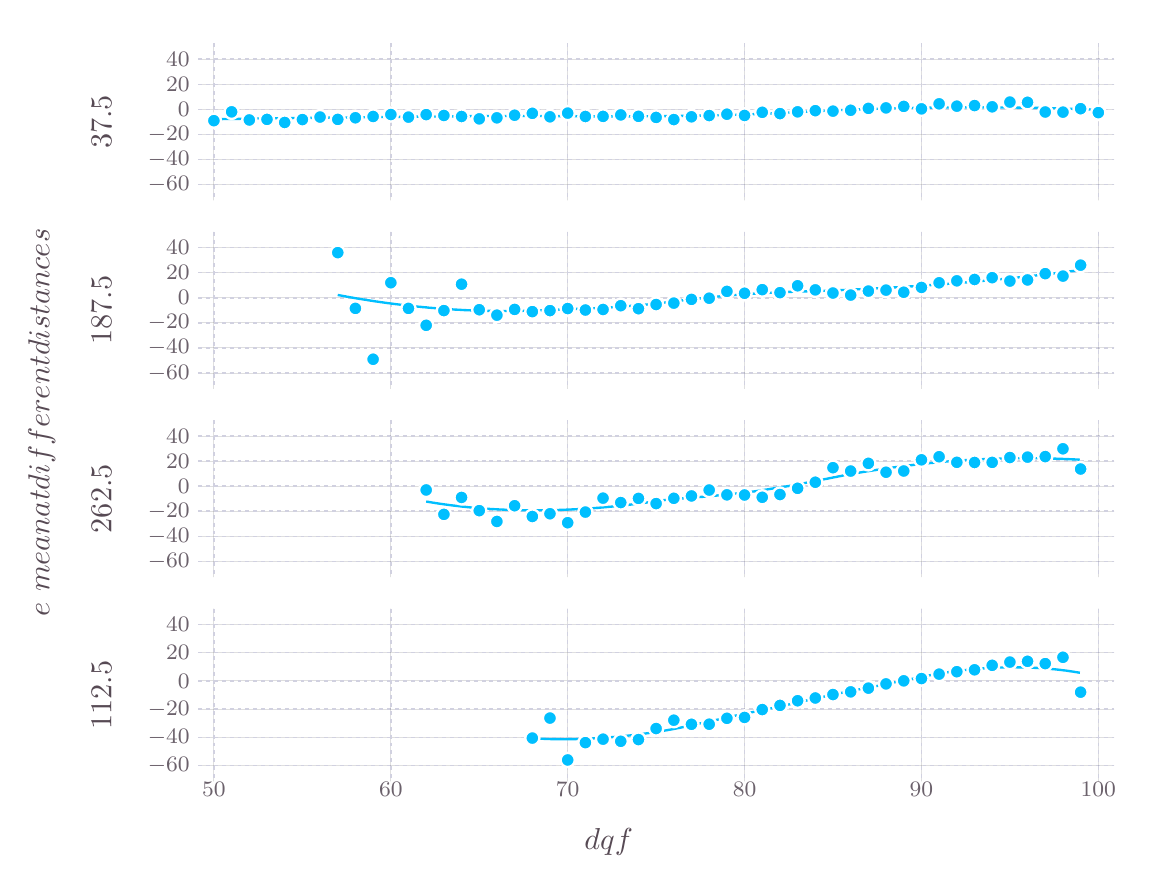
\begin{tikzpicture}[x=1mm,y=-1mm]
\definecolor{mycolor000000}{rgb}{0,0,0}
\definecolor{mycolorD0D0E0}{rgb}{0.82,0.82,0.88}
\definecolor{mycolor564A55}{rgb}{0.34,0.29,0.33}
\definecolor{mycolor6C606B}{rgb}{0.42,0.38,0.42}
\definecolor{mycolor00BFFF}{rgb}{0,0.75,1}
\definecolor{mycolor000000}{rgb}{0,0,0}
\definecolor{mycolorFFFFFF}{rgb}{1,1,1}
\begin{scope}
\begin{scope}
\draw (78.81,108.39) node [text=mycolor564A55,draw=mycolor000000,draw opacity=0,rotate around={-0: (0,1.81)},inner sep=0.0]{\fontsize{3.88mm}{4.66mm}\selectfont $\text{dqf}$};
\end{scope}
\begin{scope}
\clip  (12.61,5) -- (145,5) -- (145,105.39) -- (12.61,105.39);
\begin{scope}
\clip  (12.61,5) -- (145,5) -- (145,105.39) -- (12.61,105.39);
\begin{scope}
\clip  (12.61,5) -- (145,5) -- (145,105.39) -- (12.61,105.39);
\draw (28.68,101.72) node [text=mycolor6C606B,rotate around={-0: (56.16,1.34)},inner sep=0.0]{\fontsize{2.82mm}{3.39mm}\selectfont $\text{50}$};
\draw (51.15,101.72) node [text=mycolor6C606B,rotate around={-0: (33.69,1.34)},inner sep=0.0]{\fontsize{2.82mm}{3.39mm}\selectfont $\text{60}$};
\draw (73.61,101.72) node [text=mycolor6C606B,rotate around={-0: (11.23,1.34)},inner sep=0.0]{\fontsize{2.82mm}{3.39mm}\selectfont $\text{70}$};
\draw (96.07,101.72) node [text=mycolor6C606B,rotate around={-0: (-11.23,1.34)},inner sep=0.0]{\fontsize{2.82mm}{3.39mm}\selectfont $\text{80}$};
\draw (118.54,101.72) node [text=mycolor6C606B,rotate around={-0: (-33.7,1.34)},inner sep=0.0]{\fontsize{2.82mm}{3.39mm}\selectfont $\text{90}$};
\draw (141,101.72) node [text=mycolor6C606B,rotate around={-0: (-56.16,1.34)},inner sep=0.0]{\fontsize{2.82mm}{3.39mm}\selectfont $\text{100}$};
\end{scope}
\begin{scope}
\clip  (26.68,78.79) -- (143,78.79) -- (143,100.72) -- (26.68,100.72);
\begin{scope}
\clip  (26.68,78.79) -- (143,78.79) -- (143,100.72) -- (26.68,100.72);
\path [fill=mycolor000000,fill opacity=0,draw=mycolor000000,draw opacity=0] (26.68,78.79) rectangle +(116.32,21.93);
\end{scope}
\begin{scope}
[dash pattern=on 0.5mm off 0.5mm,line width=0.2mm]
\path [fill=mycolor000000,draw=mycolorD0D0E0]  (26.68,98.72) -- (143,98.72);
\path [fill=mycolor000000,draw=mycolorD0D0E0]  (26.68,95.13) -- (143,95.13);
\path [fill=mycolor000000,draw=mycolorD0D0E0]  (26.68,91.54) -- (143,91.54);
\path [fill=mycolor000000,draw=mycolorD0D0E0]  (26.68,87.96) -- (143,87.96);
\path [fill=mycolor000000,draw=mycolorD0D0E0]  (26.68,84.37) -- (143,84.37);
\path [fill=mycolor000000,draw=mycolorD0D0E0]  (26.68,80.79) -- (143,80.79);
\end{scope}
\begin{scope}
[dash pattern=on 0.5mm off 0.5mm,line width=0.2mm]
\path [fill=mycolor000000,draw=mycolorD0D0E0]  (28.68,78.79) -- (28.68,100.72);
\path [fill=mycolor000000,draw=mycolorD0D0E0]  (51.15,78.79) -- (51.15,100.72);
\path [fill=mycolor000000,draw=mycolorD0D0E0]  (73.61,78.79) -- (73.61,100.72);
\path [fill=mycolor000000,draw=mycolorD0D0E0]  (96.07,78.79) -- (96.07,100.72);
\path [fill=mycolor000000,draw=mycolorD0D0E0]  (118.54,78.79) -- (118.54,100.72);
\path [fill=mycolor000000,draw=mycolorD0D0E0]  (141,78.79) -- (141,100.72);
\end{scope}
\begin{scope}
\begin{scope}
[line width=0.3mm]
\path [fill=mycolor000000,fill opacity=0,draw=mycolor00BFFF]  (69.12,95.24) -- (69.21,95.25) -- (69.3,95.25) -- (69.4,95.26) -- (69.49,95.26) -- (69.58,95.27) -- (69.68,95.27) -- (69.77,95.28) -- (69.86,95.28) -- (69.95,95.29) -- (70.05,95.29) -- (70.14,95.3) -- (70.23,95.3) -- (70.33,95.31) -- (70.42,95.31) -- (70.51,95.31) -- (70.6,95.32) -- (70.7,95.32) -- (70.79,95.33) -- (70.88,95.33) -- (70.97,95.33) -- (71.07,95.33) -- (71.16,95.34) -- (71.25,95.34) -- (71.35,95.34) -- (71.44,95.35) -- (71.53,95.35) -- (71.62,95.35) -- (71.72,95.35) -- (71.81,95.35) -- (71.9,95.36) -- (72,95.36) -- (72.09,95.36) -- (72.18,95.36) -- (72.27,95.36) -- (72.37,95.36) -- (72.46,95.36) -- (72.55,95.36) -- (72.65,95.36) -- (72.74,95.36) -- (72.83,95.37) -- (72.92,95.37) -- (73.02,95.37) -- (73.11,95.37) -- (73.2,95.37) -- (73.3,95.37) -- (73.39,95.36) -- (73.48,95.36) -- (73.57,95.36) -- (73.67,95.36) -- (73.76,95.36) -- (73.85,95.36) -- (73.95,95.36) -- (74.04,95.36) -- (74.13,95.36) -- (74.22,95.36) -- (74.32,95.35) -- (74.41,95.35) -- (74.5,95.35) -- (74.6,95.35) -- (74.69,95.35) -- (74.78,95.34) -- (74.87,95.34) -- (74.97,95.34) -- (75.06,95.34) -- (75.15,95.33) -- (75.25,95.33) -- (75.34,95.33) -- (75.43,95.32) -- (75.52,95.32) -- (75.62,95.32) -- (75.71,95.31) -- (75.8,95.31) -- (75.9,95.31) -- (75.99,95.3) -- (76.08,95.3) -- (76.17,95.3) -- (76.27,95.29) -- (76.36,95.29) -- (76.45,95.28) -- (76.55,95.28) -- (76.64,95.27) -- (76.73,95.27) -- (76.82,95.26) -- (76.92,95.26) -- (77.01,95.25) -- (77.1,95.25) -- (77.2,95.24) -- (77.29,95.24) -- (77.38,95.23) -- (77.47,95.23) -- (77.57,95.22) -- (77.66,95.22) -- (77.75,95.21) -- (77.85,95.2) -- (77.94,95.2) -- (78.03,95.19) -- (78.12,95.19) -- (78.22,95.18) -- (78.31,95.17) -- (78.4,95.17) -- (78.5,95.16) -- (78.59,95.15) -- (78.68,95.15) -- (78.77,95.14) -- (78.87,95.13) -- (78.96,95.12) -- (79.05,95.12) -- (79.15,95.11) -- (79.24,95.1) -- (79.33,95.09) -- (79.42,95.09) -- (79.52,95.08) -- (79.61,95.07) -- (79.7,95.06) -- (79.8,95.05) -- (79.89,95.05) -- (79.98,95.04) -- (80.07,95.03) -- (80.17,95.02) -- (80.26,95.01) -- (80.35,95) -- (80.45,94.99) -- (80.54,94.98) -- (80.63,94.97) -- (80.72,94.97) -- (80.82,94.96) -- (80.91,94.95) -- (81,94.94) -- (81.1,94.93) -- (81.19,94.92) -- (81.28,94.91) -- (81.37,94.9) -- (81.47,94.89) -- (81.56,94.88) -- (81.65,94.87) -- (81.75,94.86) -- (81.84,94.85) -- (81.93,94.84) -- (82.02,94.82) -- (82.12,94.81) -- (82.21,94.8) -- (82.3,94.79) -- (82.4,94.78) -- (82.49,94.77) -- (82.58,94.76) -- (82.67,94.75) -- (82.77,94.73) -- (82.86,94.72) -- (82.95,94.71) -- (83.05,94.7) -- (83.14,94.69) -- (83.23,94.67) -- (83.32,94.66) -- (83.42,94.65) -- (83.51,94.64) -- (83.6,94.62) -- (83.7,94.61) -- (83.79,94.6) -- (83.88,94.58) -- (83.97,94.57) -- (84.07,94.56) -- (84.16,94.54) -- (84.25,94.53) -- (84.35,94.52) -- (84.44,94.5) -- (84.53,94.49) -- (84.62,94.48) -- (84.72,94.46) -- (84.81,94.45) -- (84.9,94.43) -- (85,94.42) -- (85.09,94.41) -- (85.18,94.39) -- (85.27,94.38) -- (85.37,94.36) -- (85.46,94.35) -- (85.55,94.33) -- (85.65,94.32) -- (85.74,94.3) -- (85.83,94.29) -- (85.92,94.27) -- (86.02,94.26) -- (86.11,94.24) -- (86.2,94.22) -- (86.29,94.21) -- (86.39,94.19) -- (86.48,94.17) -- (86.57,94.16) -- (86.67,94.14) -- (86.76,94.12) -- (86.85,94.11) -- (86.94,94.09) -- (87.04,94.07) -- (87.13,94.05) -- (87.22,94.04) -- (87.32,94.02) -- (87.41,94) -- (87.5,93.98) -- (87.59,93.96) -- (87.69,93.94) -- (87.78,93.93) -- (87.87,93.91) -- (87.97,93.89) -- (88.06,93.87) -- (88.15,93.85) -- (88.24,93.83) -- (88.34,93.81) -- (88.43,93.79) -- (88.52,93.77) -- (88.62,93.76) -- (88.71,93.74) -- (88.8,93.72) -- (88.89,93.7) -- (88.99,93.68) -- (89.08,93.66) -- (89.17,93.64) -- (89.27,93.62) -- (89.36,93.6) -- (89.45,93.58) -- (89.54,93.56) -- (89.64,93.54) -- (89.73,93.52) -- (89.82,93.5) -- (89.92,93.48) -- (90.01,93.45) -- (90.1,93.43) -- (90.19,93.41) -- (90.29,93.39) -- (90.38,93.37) -- (90.47,93.35) -- (90.57,93.33) -- (90.66,93.31) -- (90.75,93.29) -- (90.84,93.27) -- (90.94,93.25) -- (91.03,93.23) -- (91.12,93.21) -- (91.22,93.19) -- (91.31,93.17) -- (91.4,93.15) -- (91.49,93.13) -- (91.59,93.11) -- (91.68,93.09) -- (91.77,93.07) -- (91.87,93.05) -- (91.96,93.03) -- (92.05,93.01) -- (92.14,92.99) -- (92.24,92.97) -- (92.33,92.95) -- (92.42,92.93) -- (92.52,92.91) -- (92.61,92.89) -- (92.7,92.87) -- (92.79,92.85) -- (92.89,92.83) -- (92.98,92.81) -- (93.07,92.79) -- (93.17,92.77) -- (93.26,92.75) -- (93.35,92.72) -- (93.44,92.7) -- (93.54,92.68) -- (93.63,92.66) -- (93.72,92.64) -- (93.82,92.62) -- (93.91,92.6) -- (94,92.58) -- (94.09,92.56) -- (94.19,92.54) -- (94.28,92.52) -- (94.37,92.5) -- (94.47,92.47) -- (94.56,92.45) -- (94.65,92.43) -- (94.74,92.41) -- (94.84,92.39) -- (94.93,92.37) -- (95.02,92.35) -- (95.12,92.33) -- (95.21,92.31) -- (95.3,92.29) -- (95.39,92.28) -- (95.49,92.26) -- (95.58,92.24) -- (95.67,92.22) -- (95.77,92.2) -- (95.86,92.18) -- (95.95,92.16) -- (96.04,92.14) -- (96.14,92.12) -- (96.23,92.1) -- (96.32,92.09) -- (96.42,92.07) -- (96.51,92.05) -- (96.6,92.03) -- (96.69,92.01) -- (96.79,91.99) -- (96.88,91.97) -- (96.97,91.95) -- (97.07,91.93) -- (97.16,91.91) -- (97.25,91.9) -- (97.34,91.88) -- (97.44,91.86) -- (97.53,91.84) -- (97.62,91.82) -- (97.72,91.8) -- (97.81,91.78) -- (97.9,91.76) -- (97.99,91.74) -- (98.09,91.73) -- (98.18,91.71) -- (98.27,91.69) -- (98.37,91.67) -- (98.46,91.65) -- (98.55,91.63) -- (98.64,91.61) -- (98.74,91.59) -- (98.83,91.57) -- (98.92,91.56) -- (99.02,91.54) -- (99.11,91.52) -- (99.2,91.5) -- (99.29,91.48) -- (99.39,91.46) -- (99.48,91.44) -- (99.57,91.42) -- (99.67,91.4) -- (99.76,91.38) -- (99.85,91.36) -- (99.94,91.34) -- (100.04,91.32) -- (100.13,91.3) -- (100.22,91.28) -- (100.32,91.26) -- (100.41,91.24) -- (100.5,91.22) -- (100.59,91.2) -- (100.69,91.18) -- (100.78,91.16) -- (100.87,91.14) -- (100.97,91.12) -- (101.06,91.09) -- (101.15,91.07) -- (101.24,91.05) -- (101.34,91.03) -- (101.43,91.01) -- (101.52,90.99) -- (101.61,90.97) -- (101.71,90.95) -- (101.8,90.93) -- (101.89,90.91) -- (101.99,90.89) -- (102.08,90.87) -- (102.17,90.85) -- (102.26,90.83) -- (102.36,90.8) -- (102.45,90.78) -- (102.54,90.76) -- (102.64,90.74) -- (102.73,90.72) -- (102.82,90.7) -- (102.91,90.68) -- (103.01,90.66) -- (103.1,90.64) -- (103.19,90.62) -- (103.29,90.6) -- (103.38,90.58) -- (103.47,90.56) -- (103.56,90.54) -- (103.66,90.51) -- (103.75,90.49) -- (103.84,90.47) -- (103.94,90.45) -- (104.03,90.43) -- (104.12,90.41) -- (104.21,90.39) -- (104.31,90.37) -- (104.4,90.35) -- (104.49,90.33) -- (104.59,90.31) -- (104.68,90.29) -- (104.77,90.27) -- (104.86,90.25) -- (104.96,90.23) -- (105.05,90.21) -- (105.14,90.19) -- (105.24,90.17) -- (105.33,90.14) -- (105.42,90.12) -- (105.51,90.1) -- (105.61,90.08) -- (105.7,90.06) -- (105.79,90.04) -- (105.89,90.02) -- (105.98,90) -- (106.07,89.98) -- (106.16,89.96) -- (106.26,89.94) -- (106.35,89.92) -- (106.44,89.9) -- (106.54,89.88) -- (106.63,89.86) -- (106.72,89.84) -- (106.81,89.82) -- (106.91,89.8) -- (107,89.78) -- (107.09,89.75) -- (107.19,89.73) -- (107.28,89.71) -- (107.37,89.69) -- (107.46,89.67) -- (107.56,89.65) -- (107.65,89.63) -- (107.74,89.61) -- (107.84,89.59) -- (107.93,89.57) -- (108.02,89.55) -- (108.11,89.53) -- (108.21,89.51) -- (108.3,89.49) -- (108.39,89.47) -- (108.49,89.45) -- (108.58,89.43) -- (108.67,89.42) -- (108.76,89.4) -- (108.86,89.38) -- (108.95,89.36) -- (109.04,89.34) -- (109.14,89.32) -- (109.23,89.3) -- (109.32,89.29) -- (109.41,89.27) -- (109.51,89.25) -- (109.6,89.23) -- (109.69,89.21) -- (109.79,89.2) -- (109.88,89.18) -- (109.97,89.16) -- (110.06,89.14) -- (110.16,89.12) -- (110.25,89.11) -- (110.34,89.09) -- (110.44,89.07) -- (110.53,89.05) -- (110.62,89.03) -- (110.71,89.02) -- (110.81,89) -- (110.9,88.98) -- (110.99,88.96) -- (111.09,88.95) -- (111.18,88.93) -- (111.27,88.91) -- (111.36,88.89) -- (111.46,88.87) -- (111.55,88.86) -- (111.64,88.84) -- (111.74,88.82) -- (111.83,88.8) -- (111.92,88.79) -- (112.01,88.77) -- (112.11,88.75) -- (112.2,88.73) -- (112.29,88.72) -- (112.39,88.7) -- (112.48,88.68) -- (112.57,88.66) -- (112.66,88.65) -- (112.76,88.63) -- (112.85,88.61) -- (112.94,88.6) -- (113.04,88.58) -- (113.13,88.56) -- (113.22,88.54) -- (113.31,88.52) -- (113.41,88.5) -- (113.5,88.48) -- (113.59,88.46) -- (113.69,88.44) -- (113.78,88.42) -- (113.87,88.4) -- (113.96,88.38) -- (114.06,88.36) -- (114.15,88.34) -- (114.24,88.32) -- (114.34,88.3) -- (114.43,88.28) -- (114.52,88.26) -- (114.61,88.25) -- (114.71,88.23) -- (114.8,88.21) -- (114.89,88.19) -- (114.99,88.17) -- (115.08,88.15) -- (115.17,88.13) -- (115.26,88.11) -- (115.36,88.09) -- (115.45,88.07) -- (115.54,88.06) -- (115.64,88.04) -- (115.73,88.02) -- (115.82,88) -- (115.91,87.98) -- (116.01,87.96) -- (116.1,87.94) -- (116.19,87.93) -- (116.29,87.91) -- (116.38,87.89) -- (116.47,87.87) -- (116.56,87.85) -- (116.66,87.84) -- (116.75,87.82) -- (116.84,87.8) -- (116.93,87.78) -- (117.03,87.76) -- (117.12,87.75) -- (117.21,87.73) -- (117.31,87.71) -- (117.4,87.69) -- (117.49,87.67) -- (117.58,87.65) -- (117.68,87.64) -- (117.77,87.62) -- (117.86,87.6) -- (117.96,87.58) -- (118.05,87.56) -- (118.14,87.54) -- (118.23,87.52) -- (118.33,87.5) -- (118.42,87.48) -- (118.51,87.46) -- (118.61,87.44) -- (118.7,87.43) -- (118.79,87.41) -- (118.88,87.39) -- (118.98,87.37) -- (119.07,87.35) -- (119.16,87.33) -- (119.26,87.32) -- (119.35,87.3) -- (119.44,87.28) -- (119.53,87.26) -- (119.63,87.24) -- (119.72,87.23) -- (119.81,87.21) -- (119.91,87.19) -- (120,87.18) -- (120.09,87.16) -- (120.18,87.14) -- (120.28,87.13) -- (120.37,87.11) -- (120.46,87.09) -- (120.56,87.08) -- (120.65,87.06) -- (120.74,87.04) -- (120.83,87.03) -- (120.93,87.01) -- (121.02,87) -- (121.11,86.98) -- (121.21,86.97) -- (121.3,86.95) -- (121.39,86.94) -- (121.48,86.92) -- (121.58,86.91) -- (121.67,86.89) -- (121.76,86.88) -- (121.86,86.87) -- (121.95,86.85) -- (122.04,86.84) -- (122.13,86.83) -- (122.23,86.81) -- (122.32,86.8) -- (122.41,86.79) -- (122.51,86.77) -- (122.6,86.76) -- (122.69,86.75) -- (122.78,86.74) -- (122.88,86.72) -- (122.97,86.71) -- (123.06,86.7) -- (123.16,86.69) -- (123.25,86.68) -- (123.34,86.67) -- (123.43,86.65) -- (123.53,86.64) -- (123.62,86.63) -- (123.71,86.62) -- (123.81,86.61) -- (123.9,86.6) -- (123.99,86.59) -- (124.08,86.58) -- (124.18,86.57) -- (124.27,86.56) -- (124.36,86.55) -- (124.46,86.54) -- (124.55,86.53) -- (124.64,86.52) -- (124.73,86.51) -- (124.83,86.5) -- (124.92,86.49) -- (125.01,86.48) -- (125.11,86.47) -- (125.2,86.46) -- (125.29,86.46) -- (125.38,86.45) -- (125.48,86.44) -- (125.57,86.43) -- (125.66,86.42) -- (125.76,86.42) -- (125.85,86.41) -- (125.94,86.4) -- (126.03,86.39) -- (126.13,86.39) -- (126.22,86.38) -- (126.31,86.37) -- (126.41,86.37) -- (126.5,86.36) -- (126.59,86.36) -- (126.68,86.35) -- (126.78,86.34) -- (126.87,86.34) -- (126.96,86.33) -- (127.06,86.33) -- (127.15,86.32) -- (127.24,86.32) -- (127.33,86.31) -- (127.43,86.31) -- (127.52,86.3) -- (127.61,86.3) -- (127.71,86.29) -- (127.8,86.29) -- (127.89,86.28) -- (127.98,86.28) -- (128.08,86.28) -- (128.17,86.27) -- (128.26,86.27) -- (128.36,86.27) -- (128.45,86.26) -- (128.54,86.26) -- (128.63,86.26) -- (128.73,86.25) -- (128.82,86.25) -- (128.91,86.25) -- (129.01,86.25) -- (129.1,86.24) -- (129.19,86.24) -- (129.28,86.24) -- (129.38,86.24) -- (129.47,86.24) -- (129.56,86.24) -- (129.66,86.24) -- (129.75,86.23) -- (129.84,86.23) -- (129.93,86.23) -- (130.03,86.23) -- (130.12,86.23) -- (130.21,86.23) -- (130.31,86.23) -- (130.4,86.23) -- (130.49,86.23) -- (130.58,86.23) -- (130.68,86.24) -- (130.77,86.24) -- (130.86,86.24) -- (130.96,86.24) -- (131.05,86.24) -- (131.14,86.24) -- (131.23,86.24) -- (131.33,86.24) -- (131.42,86.25) -- (131.51,86.25) -- (131.61,86.25) -- (131.7,86.25) -- (131.79,86.25) -- (131.88,86.26) -- (131.98,86.26) -- (132.07,86.26) -- (132.16,86.27) -- (132.25,86.27) -- (132.35,86.27) -- (132.44,86.28) -- (132.53,86.28) -- (132.63,86.28) -- (132.72,86.29) -- (132.81,86.29) -- (132.9,86.3) -- (133,86.3) -- (133.09,86.3) -- (133.18,86.31) -- (133.28,86.31) -- (133.37,86.32) -- (133.46,86.33) -- (133.55,86.33) -- (133.65,86.34) -- (133.74,86.34) -- (133.83,86.35) -- (133.93,86.36) -- (134.02,86.36) -- (134.11,86.37) -- (134.2,86.38) -- (134.3,86.38) -- (134.39,86.39) -- (134.48,86.4) -- (134.58,86.41) -- (134.67,86.41) -- (134.76,86.42) -- (134.85,86.43) -- (134.95,86.44) -- (135.04,86.45) -- (135.13,86.46) -- (135.23,86.46) -- (135.32,86.47) -- (135.41,86.48) -- (135.5,86.49) -- (135.6,86.5) -- (135.69,86.51) -- (135.78,86.52) -- (135.88,86.53) -- (135.97,86.54) -- (136.06,86.55) -- (136.15,86.56) -- (136.25,86.57) -- (136.34,86.58) -- (136.43,86.6) -- (136.53,86.61) -- (136.62,86.62) -- (136.71,86.63) -- (136.8,86.64) -- (136.9,86.65) -- (136.99,86.67) -- (137.08,86.68) -- (137.18,86.69) -- (137.27,86.71) -- (137.36,86.72) -- (137.45,86.73) -- (137.55,86.75) -- (137.64,86.76) -- (137.73,86.77) -- (137.83,86.79) -- (137.92,86.8) -- (138.01,86.82) -- (138.1,86.83) -- (138.2,86.85) -- (138.29,86.86) -- (138.38,86.88) -- (138.48,86.89) -- (138.57,86.91) -- (138.66,86.92);
\end{scope}
\begin{scope}
\begin{scope}
[line width=0.3mm]
\path [fill=mycolor00BFFF,draw=mycolorFFFFFF] (69.12,95.22) circle [radius=0.9];
\path [fill=mycolor00BFFF,draw=mycolorFFFFFF] (71.36,92.68) circle [radius=0.9];
\path [fill=mycolor00BFFF,draw=mycolorFFFFFF] (73.61,98) circle [radius=0.9];
\path [fill=mycolor00BFFF,draw=mycolorFFFFFF] (75.86,95.8) circle [radius=0.9];
\path [fill=mycolor00BFFF,draw=mycolorFFFFFF] (78.1,95.36) circle [radius=0.9];
\path [fill=mycolor00BFFF,draw=mycolorFFFFFF] (80.35,95.63) circle [radius=0.9];
\path [fill=mycolor00BFFF,draw=mycolorFFFFFF] (82.6,95.41) circle [radius=0.9];
\path [fill=mycolor00BFFF,draw=mycolorFFFFFF] (84.84,94.01) circle [radius=0.9];
\path [fill=mycolor00BFFF,draw=mycolorFFFFFF] (87.09,92.95) circle [radius=0.9];
\path [fill=mycolor00BFFF,draw=mycolorFFFFFF] (89.33,93.47) circle [radius=0.9];
\path [fill=mycolor00BFFF,draw=mycolorFFFFFF] (91.58,93.46) circle [radius=0.9];
\path [fill=mycolor00BFFF,draw=mycolorFFFFFF] (93.83,92.71) circle [radius=0.9];
\path [fill=mycolor00BFFF,draw=mycolorFFFFFF] (96.07,92.6) circle [radius=0.9];
\path [fill=mycolor00BFFF,draw=mycolorFFFFFF] (98.32,91.6) circle [radius=0.9];
\path [fill=mycolor00BFFF,draw=mycolorFFFFFF] (100.57,91.07) circle [radius=0.9];
\path [fill=mycolor00BFFF,draw=mycolorFFFFFF] (102.81,90.48) circle [radius=0.9];
\path [fill=mycolor00BFFF,draw=mycolorFFFFFF] (105.06,90.13) circle [radius=0.9];
\path [fill=mycolor00BFFF,draw=mycolorFFFFFF] (107.3,89.69) circle [radius=0.9];
\path [fill=mycolor00BFFF,draw=mycolorFFFFFF] (109.55,89.35) circle [radius=0.9];
\path [fill=mycolor00BFFF,draw=mycolorFFFFFF] (111.8,88.88) circle [radius=0.9];
\path [fill=mycolor00BFFF,draw=mycolorFFFFFF] (114.04,88.34) circle [radius=0.9];
\path [fill=mycolor00BFFF,draw=mycolorFFFFFF] (116.29,87.95) circle [radius=0.9];
\path [fill=mycolor00BFFF,draw=mycolorFFFFFF] (118.54,87.66) circle [radius=0.9];
\path [fill=mycolor00BFFF,draw=mycolorFFFFFF] (120.78,87.1) circle [radius=0.9];
\path [fill=mycolor00BFFF,draw=mycolorFFFFFF] (123.03,86.79) circle [radius=0.9];
\path [fill=mycolor00BFFF,draw=mycolorFFFFFF] (125.28,86.55) circle [radius=0.9];
\path [fill=mycolor00BFFF,draw=mycolorFFFFFF] (127.52,85.98) circle [radius=0.9];
\path [fill=mycolor00BFFF,draw=mycolorFFFFFF] (129.77,85.57) circle [radius=0.9];
\path [fill=mycolor00BFFF,draw=mycolorFFFFFF] (132.01,85.47) circle [radius=0.9];
\path [fill=mycolor00BFFF,draw=mycolorFFFFFF] (134.26,85.76) circle [radius=0.9];
\path [fill=mycolor00BFFF,draw=mycolorFFFFFF] (136.51,84.96) circle [radius=0.9];
\path [fill=mycolor00BFFF,draw=mycolorFFFFFF] (138.75,89.39) circle [radius=0.9];
\end{scope}
\end{scope}
\end{scope}
\end{scope}
\begin{scope}
\draw (25.68,98.72) node [text=mycolor6C606B,rotate around={-0: (-2.23,-8.96)},left,inner sep=0.0]{\fontsize{2.82mm}{3.39mm}\selectfont $\text{-60}$};
\draw (25.68,95.13) node [text=mycolor6C606B,rotate around={-0: (-2.23,-5.38)},left,inner sep=0.0]{\fontsize{2.82mm}{3.39mm}\selectfont $\text{-40}$};
\draw (25.68,91.54) node [text=mycolor6C606B,rotate around={-0: (-2.23,-1.79)},left,inner sep=0.0]{\fontsize{2.82mm}{3.39mm}\selectfont $\text{-20}$};
\draw (25.68,87.96) node [text=mycolor6C606B,rotate around={-0: (-2.23,1.79)},left,inner sep=0.0]{\fontsize{2.82mm}{3.39mm}\selectfont $\text{0}$};
\draw (25.68,84.37) node [text=mycolor6C606B,rotate around={-0: (-2.23,5.38)},left,inner sep=0.0]{\fontsize{2.82mm}{3.39mm}\selectfont $\text{20}$};
\draw (25.68,80.79) node [text=mycolor6C606B,rotate around={-0: (-2.23,8.96)},left,inner sep=0.0]{\fontsize{2.82mm}{3.39mm}\selectfont $\text{40}$};
\end{scope}
\begin{scope}
\draw (16.42,87.75) node [text=mycolor564A55,draw=mycolor000000,draw opacity=0,rotate around={90: (0,2)},inner sep=0.0]{\fontsize{3.88mm}{4.66mm}\selectfont $\text{112.5}$};
\end{scope}
\begin{scope}
\clip  (26.68,54.86) -- (143,54.86) -- (143,74.79) -- (26.68,74.79);
\begin{scope}
\clip  (26.68,54.86) -- (143,54.86) -- (143,74.79) -- (26.68,74.79);
\path [fill=mycolor000000,fill opacity=0,draw=mycolor000000,draw opacity=0] (26.68,54.86) rectangle +(116.32,19.93);
\end{scope}
\begin{scope}
[dash pattern=on 0.5mm off 0.5mm,line width=0.2mm]
\path [fill=mycolor000000,draw=mycolorD0D0E0]  (26.68,72.79) -- (143,72.79);
\path [fill=mycolor000000,draw=mycolorD0D0E0]  (26.68,69.6) -- (143,69.6);
\path [fill=mycolor000000,draw=mycolorD0D0E0]  (26.68,66.41) -- (143,66.41);
\path [fill=mycolor000000,draw=mycolorD0D0E0]  (26.68,63.23) -- (143,63.23);
\path [fill=mycolor000000,draw=mycolorD0D0E0]  (26.68,60.04) -- (143,60.04);
\path [fill=mycolor000000,draw=mycolorD0D0E0]  (26.68,56.86) -- (143,56.86);
\end{scope}
\begin{scope}
[dash pattern=on 0.5mm off 0.5mm,line width=0.2mm]
\path [fill=mycolor000000,draw=mycolorD0D0E0]  (28.68,54.86) -- (28.68,74.79);
\path [fill=mycolor000000,draw=mycolorD0D0E0]  (51.15,54.86) -- (51.15,74.79);
\path [fill=mycolor000000,draw=mycolorD0D0E0]  (73.61,54.86) -- (73.61,74.79);
\path [fill=mycolor000000,draw=mycolorD0D0E0]  (96.07,54.86) -- (96.07,74.79);
\path [fill=mycolor000000,draw=mycolorD0D0E0]  (118.54,54.86) -- (118.54,74.79);
\path [fill=mycolor000000,draw=mycolorD0D0E0]  (141,54.86) -- (141,74.79);
\end{scope}
\begin{scope}
\begin{scope}
[line width=0.3mm]
\path [fill=mycolor000000,fill opacity=0,draw=mycolor00BFFF]  (55.64,65.18) -- (55.75,65.2) -- (55.86,65.22) -- (55.97,65.23) -- (56.08,65.25) -- (56.19,65.27) -- (56.31,65.29) -- (56.42,65.31) -- (56.53,65.33) -- (56.64,65.34) -- (56.75,65.36) -- (56.86,65.38) -- (56.97,65.4) -- (57.08,65.41) -- (57.19,65.43) -- (57.3,65.45) -- (57.41,65.46) -- (57.52,65.48) -- (57.63,65.49) -- (57.75,65.51) -- (57.86,65.53) -- (57.97,65.54) -- (58.08,65.56) -- (58.19,65.57) -- (58.3,65.59) -- (58.41,65.6) -- (58.52,65.62) -- (58.63,65.63) -- (58.74,65.65) -- (58.85,65.66) -- (58.96,65.67) -- (59.08,65.69) -- (59.19,65.7) -- (59.3,65.71) -- (59.41,65.73) -- (59.52,65.74) -- (59.63,65.75) -- (59.74,65.77) -- (59.85,65.78) -- (59.96,65.79) -- (60.07,65.8) -- (60.18,65.82) -- (60.29,65.83) -- (60.41,65.84) -- (60.52,65.85) -- (60.63,65.86) -- (60.74,65.87) -- (60.85,65.89) -- (60.96,65.9) -- (61.07,65.91) -- (61.18,65.92) -- (61.29,65.93) -- (61.4,65.94) -- (61.51,65.95) -- (61.62,65.96) -- (61.74,65.97) -- (61.85,65.98) -- (61.96,65.99) -- (62.07,66) -- (62.18,66.01) -- (62.29,66.01) -- (62.4,66.02) -- (62.51,66.03) -- (62.62,66.04) -- (62.73,66.05) -- (62.84,66.06) -- (62.95,66.07) -- (63.07,66.07) -- (63.18,66.08) -- (63.29,66.09) -- (63.4,66.1) -- (63.51,66.1) -- (63.62,66.11) -- (63.73,66.12) -- (63.84,66.13) -- (63.95,66.13) -- (64.06,66.14) -- (64.17,66.15) -- (64.28,66.15) -- (64.39,66.16) -- (64.51,66.16) -- (64.62,66.17) -- (64.73,66.18) -- (64.84,66.18) -- (64.95,66.19) -- (65.06,66.19) -- (65.17,66.2) -- (65.28,66.2) -- (65.39,66.21) -- (65.5,66.21) -- (65.61,66.22) -- (65.72,66.22) -- (65.84,66.23) -- (65.95,66.23) -- (66.06,66.23) -- (66.17,66.24) -- (66.28,66.24) -- (66.39,66.24) -- (66.5,66.25) -- (66.61,66.25) -- (66.72,66.25) -- (66.83,66.26) -- (66.94,66.26) -- (67.05,66.26) -- (67.17,66.27) -- (67.28,66.27) -- (67.39,66.27) -- (67.5,66.27) -- (67.61,66.28) -- (67.72,66.28) -- (67.83,66.28) -- (67.94,66.28) -- (68.05,66.28) -- (68.16,66.28) -- (68.27,66.29) -- (68.38,66.29) -- (68.5,66.29) -- (68.61,66.29) -- (68.72,66.29) -- (68.83,66.29) -- (68.94,66.29) -- (69.05,66.29) -- (69.16,66.29) -- (69.27,66.29) -- (69.38,66.29) -- (69.49,66.29) -- (69.6,66.29) -- (69.71,66.29) -- (69.83,66.29) -- (69.94,66.29) -- (70.05,66.29) -- (70.16,66.29) -- (70.27,66.29) -- (70.38,66.29) -- (70.49,66.29) -- (70.6,66.29) -- (70.71,66.29) -- (70.82,66.28) -- (70.93,66.28) -- (71.04,66.28) -- (71.15,66.28) -- (71.27,66.28) -- (71.38,66.28) -- (71.49,66.27) -- (71.6,66.27) -- (71.71,66.27) -- (71.82,66.27) -- (71.93,66.26) -- (72.04,66.26) -- (72.15,66.26) -- (72.26,66.25) -- (72.37,66.25) -- (72.48,66.25) -- (72.6,66.24) -- (72.71,66.24) -- (72.82,66.24) -- (72.93,66.23) -- (73.04,66.23) -- (73.15,66.23) -- (73.26,66.22) -- (73.37,66.22) -- (73.48,66.21) -- (73.59,66.21) -- (73.7,66.2) -- (73.81,66.2) -- (73.93,66.19) -- (74.04,66.19) -- (74.15,66.18) -- (74.26,66.18) -- (74.37,66.17) -- (74.48,66.17) -- (74.59,66.16) -- (74.7,66.16) -- (74.81,66.15) -- (74.92,66.15) -- (75.03,66.14) -- (75.14,66.13) -- (75.26,66.13) -- (75.37,66.12) -- (75.48,66.11) -- (75.59,66.11) -- (75.7,66.1) -- (75.81,66.09) -- (75.92,66.09) -- (76.03,66.08) -- (76.14,66.07) -- (76.25,66.07) -- (76.36,66.06) -- (76.47,66.05) -- (76.58,66.04) -- (76.7,66.03) -- (76.81,66.03) -- (76.92,66.02) -- (77.03,66.01) -- (77.14,66) -- (77.25,65.99) -- (77.36,65.99) -- (77.47,65.98) -- (77.58,65.97) -- (77.69,65.96) -- (77.8,65.95) -- (77.91,65.94) -- (78.03,65.93) -- (78.14,65.92) -- (78.25,65.91) -- (78.36,65.9) -- (78.47,65.89) -- (78.58,65.88) -- (78.69,65.87) -- (78.8,65.86) -- (78.91,65.85) -- (79.02,65.84) -- (79.13,65.83) -- (79.24,65.82) -- (79.36,65.81) -- (79.47,65.8) -- (79.58,65.79) -- (79.69,65.78) -- (79.8,65.77) -- (79.91,65.75) -- (80.02,65.74) -- (80.13,65.73) -- (80.24,65.72) -- (80.35,65.71) -- (80.46,65.7) -- (80.57,65.68) -- (80.69,65.67) -- (80.8,65.66) -- (80.91,65.65) -- (81.02,65.64) -- (81.13,65.62) -- (81.24,65.61) -- (81.35,65.6) -- (81.46,65.58) -- (81.57,65.57) -- (81.68,65.56) -- (81.79,65.54) -- (81.9,65.53) -- (82.02,65.52) -- (82.13,65.5) -- (82.24,65.49) -- (82.35,65.48) -- (82.46,65.46) -- (82.57,65.45) -- (82.68,65.43) -- (82.79,65.42) -- (82.9,65.41) -- (83.01,65.39) -- (83.12,65.38) -- (83.23,65.36) -- (83.34,65.35) -- (83.46,65.33) -- (83.57,65.32) -- (83.68,65.3) -- (83.79,65.29) -- (83.9,65.27) -- (84.01,65.26) -- (84.12,65.24) -- (84.23,65.23) -- (84.34,65.21) -- (84.45,65.19) -- (84.56,65.18) -- (84.67,65.16) -- (84.79,65.15) -- (84.9,65.13) -- (85.01,65.12) -- (85.12,65.1) -- (85.23,65.09) -- (85.34,65.07) -- (85.45,65.05) -- (85.56,65.04) -- (85.67,65.02) -- (85.78,65.01) -- (85.89,64.99) -- (86,64.98) -- (86.12,64.97) -- (86.23,64.96) -- (86.34,64.95) -- (86.45,64.94) -- (86.56,64.93) -- (86.67,64.92) -- (86.78,64.91) -- (86.89,64.9) -- (87,64.89) -- (87.11,64.88) -- (87.22,64.87) -- (87.33,64.86) -- (87.45,64.85) -- (87.56,64.84) -- (87.67,64.83) -- (87.78,64.82) -- (87.89,64.81) -- (88,64.8) -- (88.11,64.79) -- (88.22,64.78) -- (88.33,64.77) -- (88.44,64.76) -- (88.55,64.75) -- (88.66,64.74) -- (88.78,64.73) -- (88.89,64.72) -- (89,64.71) -- (89.11,64.7) -- (89.22,64.69) -- (89.33,64.68) -- (89.44,64.67) -- (89.55,64.66) -- (89.66,64.66) -- (89.77,64.65) -- (89.88,64.64) -- (89.99,64.63) -- (90.1,64.62) -- (90.22,64.62) -- (90.33,64.61) -- (90.44,64.6) -- (90.55,64.59) -- (90.66,64.59) -- (90.77,64.58) -- (90.88,64.57) -- (90.99,64.56) -- (91.1,64.55) -- (91.21,64.54) -- (91.32,64.54) -- (91.43,64.53) -- (91.55,64.52) -- (91.66,64.51) -- (91.77,64.5) -- (91.88,64.49) -- (91.99,64.47) -- (92.1,64.46) -- (92.21,64.45) -- (92.32,64.44) -- (92.43,64.43) -- (92.54,64.42) -- (92.65,64.41) -- (92.76,64.39) -- (92.88,64.38) -- (92.99,64.37) -- (93.1,64.36) -- (93.21,64.35) -- (93.32,64.34) -- (93.43,64.33) -- (93.54,64.31) -- (93.65,64.3) -- (93.76,64.29) -- (93.87,64.28) -- (93.98,64.27) -- (94.09,64.26) -- (94.21,64.24) -- (94.32,64.23) -- (94.43,64.22) -- (94.54,64.21) -- (94.65,64.2) -- (94.76,64.19) -- (94.87,64.17) -- (94.98,64.16) -- (95.09,64.15) -- (95.2,64.14) -- (95.31,64.13) -- (95.42,64.11) -- (95.54,64.1) -- (95.65,64.09) -- (95.76,64.08) -- (95.87,64.06) -- (95.98,64.05) -- (96.09,64.04) -- (96.2,64.03) -- (96.31,64.01) -- (96.42,64) -- (96.53,63.99) -- (96.64,63.97) -- (96.75,63.96) -- (96.86,63.95) -- (96.98,63.94) -- (97.09,63.92) -- (97.2,63.91) -- (97.31,63.89) -- (97.42,63.88) -- (97.53,63.86) -- (97.64,63.84) -- (97.75,63.83) -- (97.86,63.81) -- (97.97,63.79) -- (98.08,63.77) -- (98.19,63.76) -- (98.31,63.74) -- (98.42,63.72) -- (98.53,63.71) -- (98.64,63.69) -- (98.75,63.67) -- (98.86,63.65) -- (98.97,63.64) -- (99.08,63.62) -- (99.19,63.6) -- (99.3,63.58) -- (99.41,63.57) -- (99.52,63.55) -- (99.64,63.53) -- (99.75,63.51) -- (99.86,63.5) -- (99.97,63.48) -- (100.08,63.46) -- (100.19,63.44) -- (100.3,63.43) -- (100.41,63.41) -- (100.52,63.39) -- (100.63,63.37) -- (100.74,63.36) -- (100.85,63.34) -- (100.97,63.32) -- (101.08,63.3) -- (101.19,63.29) -- (101.3,63.27) -- (101.41,63.25) -- (101.52,63.23) -- (101.63,63.22) -- (101.74,63.2) -- (101.85,63.18) -- (101.96,63.16) -- (102.07,63.14) -- (102.18,63.12) -- (102.3,63.1) -- (102.41,63.08) -- (102.52,63.06) -- (102.63,63.04) -- (102.74,63.02) -- (102.85,63) -- (102.96,62.97) -- (103.07,62.95) -- (103.18,62.93) -- (103.29,62.91) -- (103.4,62.89) -- (103.51,62.87) -- (103.62,62.85) -- (103.74,62.83) -- (103.85,62.81) -- (103.96,62.79) -- (104.07,62.77) -- (104.18,62.75) -- (104.29,62.73) -- (104.4,62.7) -- (104.51,62.68) -- (104.62,62.66) -- (104.73,62.64) -- (104.84,62.62) -- (104.95,62.6) -- (105.07,62.58) -- (105.18,62.56) -- (105.29,62.53) -- (105.4,62.51) -- (105.51,62.49) -- (105.62,62.47) -- (105.73,62.45) -- (105.84,62.42) -- (105.95,62.4) -- (106.06,62.38) -- (106.17,62.36) -- (106.28,62.33) -- (106.4,62.31) -- (106.51,62.29) -- (106.62,62.27) -- (106.73,62.25) -- (106.84,62.22) -- (106.95,62.2) -- (107.06,62.18) -- (107.17,62.16) -- (107.28,62.13) -- (107.39,62.11) -- (107.5,62.09) -- (107.61,62.07) -- (107.73,62.05) -- (107.84,62.02) -- (107.95,62) -- (108.06,61.98) -- (108.17,61.96) -- (108.28,61.94) -- (108.39,61.92) -- (108.5,61.89) -- (108.61,61.87) -- (108.72,61.85) -- (108.83,61.83) -- (108.94,61.81) -- (109.05,61.79) -- (109.17,61.77) -- (109.28,61.75) -- (109.39,61.73) -- (109.5,61.71) -- (109.61,61.69) -- (109.72,61.67) -- (109.83,61.65) -- (109.94,61.63) -- (110.05,61.61) -- (110.16,61.59) -- (110.27,61.57) -- (110.38,61.55) -- (110.5,61.53) -- (110.61,61.52) -- (110.72,61.5) -- (110.83,61.48) -- (110.94,61.46) -- (111.05,61.44) -- (111.16,61.42) -- (111.27,61.41) -- (111.38,61.39) -- (111.49,61.37) -- (111.6,61.35) -- (111.71,61.33) -- (111.83,61.32) -- (111.94,61.3) -- (112.05,61.28) -- (112.16,61.26) -- (112.27,61.25) -- (112.38,61.23) -- (112.49,61.21) -- (112.6,61.2) -- (112.71,61.18) -- (112.82,61.16) -- (112.93,61.15) -- (113.04,61.13) -- (113.16,61.11) -- (113.27,61.1) -- (113.38,61.08) -- (113.49,61.06) -- (113.6,61.05) -- (113.71,61.03) -- (113.82,61.02) -- (113.93,61) -- (114.04,60.98) -- (114.15,60.97) -- (114.26,60.95) -- (114.37,60.94) -- (114.49,60.92) -- (114.6,60.9) -- (114.71,60.89) -- (114.82,60.87) -- (114.93,60.86) -- (115.04,60.84) -- (115.15,60.83) -- (115.26,60.81) -- (115.37,60.8) -- (115.48,60.78) -- (115.59,60.77) -- (115.7,60.75) -- (115.81,60.74) -- (115.93,60.72) -- (116.04,60.71) -- (116.15,60.7) -- (116.26,60.68) -- (116.37,60.67) -- (116.48,60.65) -- (116.59,60.64) -- (116.7,60.63) -- (116.81,60.61) -- (116.92,60.6) -- (117.03,60.59) -- (117.14,60.57) -- (117.26,60.56) -- (117.37,60.55) -- (117.48,60.53) -- (117.59,60.52) -- (117.7,60.51) -- (117.81,60.49) -- (117.92,60.48) -- (118.03,60.47) -- (118.14,60.46) -- (118.25,60.44) -- (118.36,60.43) -- (118.47,60.42) -- (118.59,60.41) -- (118.7,60.4) -- (118.81,60.38) -- (118.92,60.37) -- (119.03,60.36) -- (119.14,60.35) -- (119.25,60.34) -- (119.36,60.32) -- (119.47,60.31) -- (119.58,60.3) -- (119.69,60.29) -- (119.8,60.28) -- (119.92,60.27) -- (120.03,60.26) -- (120.14,60.25) -- (120.25,60.24) -- (120.36,60.22) -- (120.47,60.21) -- (120.58,60.2) -- (120.69,60.19) -- (120.8,60.18) -- (120.91,60.17) -- (121.02,60.16) -- (121.13,60.15) -- (121.25,60.14) -- (121.36,60.13) -- (121.47,60.12) -- (121.58,60.11) -- (121.69,60.1) -- (121.8,60.1) -- (121.91,60.09) -- (122.02,60.08) -- (122.13,60.07) -- (122.24,60.06) -- (122.35,60.05) -- (122.46,60.04) -- (122.57,60.03) -- (122.69,60.02) -- (122.8,60.02) -- (122.91,60.01) -- (123.02,60) -- (123.13,59.99) -- (123.24,59.98) -- (123.35,59.98) -- (123.46,59.97) -- (123.57,59.96) -- (123.68,59.95) -- (123.79,59.95) -- (123.9,59.94) -- (124.02,59.93) -- (124.13,59.92) -- (124.24,59.92) -- (124.35,59.91) -- (124.46,59.9) -- (124.57,59.9) -- (124.68,59.89) -- (124.79,59.88) -- (124.9,59.88) -- (125.01,59.87) -- (125.12,59.86) -- (125.23,59.86) -- (125.35,59.85) -- (125.46,59.85) -- (125.57,59.84) -- (125.68,59.83) -- (125.79,59.83) -- (125.9,59.82) -- (126.01,59.82) -- (126.12,59.81) -- (126.23,59.81) -- (126.34,59.8) -- (126.45,59.8) -- (126.56,59.79) -- (126.68,59.79) -- (126.79,59.78) -- (126.9,59.78) -- (127.01,59.77) -- (127.12,59.77) -- (127.23,59.76) -- (127.34,59.76) -- (127.45,59.76) -- (127.56,59.75) -- (127.67,59.75) -- (127.78,59.74) -- (127.89,59.74) -- (128.01,59.74) -- (128.12,59.73) -- (128.23,59.73) -- (128.34,59.73) -- (128.45,59.72) -- (128.56,59.72) -- (128.67,59.72) -- (128.78,59.72) -- (128.89,59.71) -- (129,59.71) -- (129.11,59.71) -- (129.22,59.71) -- (129.33,59.7) -- (129.45,59.7) -- (129.56,59.7) -- (129.67,59.7) -- (129.78,59.7) -- (129.89,59.69) -- (130,59.69) -- (130.11,59.69) -- (130.22,59.69) -- (130.33,59.69) -- (130.44,59.69) -- (130.55,59.68) -- (130.66,59.68) -- (130.78,59.68) -- (130.89,59.68) -- (131,59.68) -- (131.11,59.68) -- (131.22,59.68) -- (131.33,59.68) -- (131.44,59.68) -- (131.55,59.68) -- (131.66,59.68) -- (131.77,59.68) -- (131.88,59.68) -- (131.99,59.68) -- (132.11,59.68) -- (132.22,59.68) -- (132.33,59.68) -- (132.44,59.68) -- (132.55,59.68) -- (132.66,59.68) -- (132.77,59.68) -- (132.88,59.68) -- (132.99,59.68) -- (133.1,59.69) -- (133.21,59.69) -- (133.32,59.69) -- (133.44,59.69) -- (133.55,59.69) -- (133.66,59.69) -- (133.77,59.69) -- (133.88,59.7) -- (133.99,59.7) -- (134.1,59.7) -- (134.21,59.7) -- (134.32,59.7) -- (134.43,59.71) -- (134.54,59.71) -- (134.65,59.71) -- (134.77,59.71) -- (134.88,59.72) -- (134.99,59.72) -- (135.1,59.72) -- (135.21,59.72) -- (135.32,59.73) -- (135.43,59.73) -- (135.54,59.73) -- (135.65,59.74) -- (135.76,59.74) -- (135.87,59.74) -- (135.98,59.75) -- (136.09,59.75) -- (136.21,59.76) -- (136.32,59.76) -- (136.43,59.76) -- (136.54,59.77) -- (136.65,59.77) -- (136.76,59.78) -- (136.87,59.78) -- (136.98,59.79) -- (137.09,59.79) -- (137.2,59.8) -- (137.31,59.8) -- (137.42,59.81) -- (137.54,59.81) -- (137.65,59.82) -- (137.76,59.82) -- (137.87,59.83) -- (137.98,59.83) -- (138.09,59.84) -- (138.2,59.84) -- (138.31,59.85) -- (138.42,59.85) -- (138.53,59.86) -- (138.64,59.87);
\end{scope}
\begin{scope}
\begin{scope}
[line width=0.3mm]
\path [fill=mycolor00BFFF,draw=mycolorFFFFFF] (55.64,63.71) circle [radius=0.9];
\path [fill=mycolor00BFFF,draw=mycolorFFFFFF] (57.89,66.81) circle [radius=0.9];
\path [fill=mycolor00BFFF,draw=mycolorFFFFFF] (60.13,64.66) circle [radius=0.9];
\path [fill=mycolor00BFFF,draw=mycolorFFFFFF] (62.38,66.34) circle [radius=0.9];
\path [fill=mycolor00BFFF,draw=mycolorFFFFFF] (64.62,67.71) circle [radius=0.9];
\path [fill=mycolor00BFFF,draw=mycolorFFFFFF] (66.87,65.71) circle [radius=0.9];
\path [fill=mycolor00BFFF,draw=mycolorFFFFFF] (69.12,67.08) circle [radius=0.9];
\path [fill=mycolor00BFFF,draw=mycolorFFFFFF] (71.36,66.73) circle [radius=0.9];
\path [fill=mycolor00BFFF,draw=mycolorFFFFFF] (73.61,67.87) circle [radius=0.9];
\path [fill=mycolor00BFFF,draw=mycolorFFFFFF] (75.86,66.52) circle [radius=0.9];
\path [fill=mycolor00BFFF,draw=mycolorFFFFFF] (78.1,64.75) circle [radius=0.9];
\path [fill=mycolor00BFFF,draw=mycolorFFFFFF] (80.35,65.31) circle [radius=0.9];
\path [fill=mycolor00BFFF,draw=mycolorFFFFFF] (82.6,64.78) circle [radius=0.9];
\path [fill=mycolor00BFFF,draw=mycolorFFFFFF] (84.84,65.44) circle [radius=0.9];
\path [fill=mycolor00BFFF,draw=mycolorFFFFFF] (87.09,64.77) circle [radius=0.9];
\path [fill=mycolor00BFFF,draw=mycolorFFFFFF] (89.33,64.47) circle [radius=0.9];
\path [fill=mycolor00BFFF,draw=mycolorFFFFFF] (91.58,63.72) circle [radius=0.9];
\path [fill=mycolor00BFFF,draw=mycolorFFFFFF] (93.83,64.33) circle [radius=0.9];
\path [fill=mycolor00BFFF,draw=mycolorFFFFFF] (96.07,64.35) circle [radius=0.9];
\path [fill=mycolor00BFFF,draw=mycolorFFFFFF] (98.32,64.64) circle [radius=0.9];
\path [fill=mycolor00BFFF,draw=mycolorFFFFFF] (100.57,64.29) circle [radius=0.9];
\path [fill=mycolor00BFFF,draw=mycolorFFFFFF] (102.81,63.5) circle [radius=0.9];
\path [fill=mycolor00BFFF,draw=mycolorFFFFFF] (105.06,62.73) circle [radius=0.9];
\path [fill=mycolor00BFFF,draw=mycolorFFFFFF] (107.3,60.88) circle [radius=0.9];
\path [fill=mycolor00BFFF,draw=mycolorFFFFFF] (109.55,61.31) circle [radius=0.9];
\path [fill=mycolor00BFFF,draw=mycolorFFFFFF] (111.8,60.33) circle [radius=0.9];
\path [fill=mycolor00BFFF,draw=mycolorFFFFFF] (114.04,61.46) circle [radius=0.9];
\path [fill=mycolor00BFFF,draw=mycolorFFFFFF] (116.29,61.3) circle [radius=0.9];
\path [fill=mycolor00BFFF,draw=mycolorFFFFFF] (118.54,59.88) circle [radius=0.9];
\path [fill=mycolor00BFFF,draw=mycolorFFFFFF] (120.78,59.49) circle [radius=0.9];
\path [fill=mycolor00BFFF,draw=mycolorFFFFFF] (123.03,60.2) circle [radius=0.9];
\path [fill=mycolor00BFFF,draw=mycolorFFFFFF] (125.28,60.22) circle [radius=0.9];
\path [fill=mycolor00BFFF,draw=mycolorFFFFFF] (127.52,60.21) circle [radius=0.9];
\path [fill=mycolor00BFFF,draw=mycolorFFFFFF] (129.77,59.59) circle [radius=0.9];
\path [fill=mycolor00BFFF,draw=mycolorFFFFFF] (132.01,59.54) circle [radius=0.9];
\path [fill=mycolor00BFFF,draw=mycolorFFFFFF] (134.26,59.47) circle [radius=0.9];
\path [fill=mycolor00BFFF,draw=mycolorFFFFFF] (136.51,58.48) circle [radius=0.9];
\path [fill=mycolor00BFFF,draw=mycolorFFFFFF] (138.75,61.05) circle [radius=0.9];
\end{scope}
\end{scope}
\end{scope}
\end{scope}
\begin{scope}
\draw (25.68,72.79) node [text=mycolor6C606B,rotate around={-0: (-2.23,-7.96)},left,inner sep=0.0]{\fontsize{2.82mm}{3.39mm}\selectfont $\text{-60}$};
\draw (25.68,69.6) node [text=mycolor6C606B,rotate around={-0: (-2.23,-4.78)},left,inner sep=0.0]{\fontsize{2.82mm}{3.39mm}\selectfont $\text{-40}$};
\draw (25.68,66.41) node [text=mycolor6C606B,rotate around={-0: (-2.23,-1.59)},left,inner sep=0.0]{\fontsize{2.82mm}{3.39mm}\selectfont $\text{-20}$};
\draw (25.68,63.23) node [text=mycolor6C606B,rotate around={-0: (-2.23,1.59)},left,inner sep=0.0]{\fontsize{2.82mm}{3.39mm}\selectfont $\text{0}$};
\draw (25.68,60.04) node [text=mycolor6C606B,rotate around={-0: (-2.23,4.78)},left,inner sep=0.0]{\fontsize{2.82mm}{3.39mm}\selectfont $\text{20}$};
\draw (25.68,56.86) node [text=mycolor6C606B,rotate around={-0: (-2.23,7.96)},left,inner sep=0.0]{\fontsize{2.82mm}{3.39mm}\selectfont $\text{40}$};
\end{scope}
\begin{scope}
\draw (16.42,62.82) node [text=mycolor564A55,draw=mycolor000000,draw opacity=0,rotate around={90: (0,2)},inner sep=0.0]{\fontsize{3.88mm}{4.66mm}\selectfont $\text{262.5}$};
\end{scope}
\begin{scope}
\clip  (26.68,30.93) -- (143,30.93) -- (143,50.86) -- (26.68,50.86);
\begin{scope}
\clip  (26.68,30.93) -- (143,30.93) -- (143,50.86) -- (26.68,50.86);
\path [fill=mycolor000000,fill opacity=0,draw=mycolor000000,draw opacity=0] (26.68,30.93) rectangle +(116.32,19.93);
\end{scope}
\begin{scope}
[dash pattern=on 0.5mm off 0.5mm,line width=0.2mm]
\path [fill=mycolor000000,draw=mycolorD0D0E0]  (26.68,48.86) -- (143,48.86);
\path [fill=mycolor000000,draw=mycolorD0D0E0]  (26.68,45.67) -- (143,45.67);
\path [fill=mycolor000000,draw=mycolorD0D0E0]  (26.68,42.49) -- (143,42.49);
\path [fill=mycolor000000,draw=mycolorD0D0E0]  (26.68,39.3) -- (143,39.3);
\path [fill=mycolor000000,draw=mycolorD0D0E0]  (26.68,36.11) -- (143,36.11);
\path [fill=mycolor000000,draw=mycolorD0D0E0]  (26.68,32.93) -- (143,32.93);
\end{scope}
\begin{scope}
[dash pattern=on 0.5mm off 0.5mm,line width=0.2mm]
\path [fill=mycolor000000,draw=mycolorD0D0E0]  (28.68,30.93) -- (28.68,50.86);
\path [fill=mycolor000000,draw=mycolorD0D0E0]  (51.15,30.93) -- (51.15,50.86);
\path [fill=mycolor000000,draw=mycolorD0D0E0]  (73.61,30.93) -- (73.61,50.86);
\path [fill=mycolor000000,draw=mycolorD0D0E0]  (96.07,30.93) -- (96.07,50.86);
\path [fill=mycolor000000,draw=mycolorD0D0E0]  (118.54,30.93) -- (118.54,50.86);
\path [fill=mycolor000000,draw=mycolorD0D0E0]  (141,30.93) -- (141,50.86);
\end{scope}
\begin{scope}
\begin{scope}
[line width=0.3mm]
\path [fill=mycolor000000,fill opacity=0,draw=mycolor00BFFF]  (44.41,38.94) -- (44.53,38.97) -- (44.66,38.99) -- (44.79,39.02) -- (44.91,39.04) -- (45.04,39.06) -- (45.16,39.09) -- (45.29,39.11) -- (45.41,39.13) -- (45.54,39.16) -- (45.67,39.18) -- (45.79,39.2) -- (45.92,39.23) -- (46.04,39.25) -- (46.17,39.27) -- (46.3,39.29) -- (46.42,39.31) -- (46.55,39.34) -- (46.67,39.36) -- (46.8,39.38) -- (46.92,39.4) -- (47.05,39.42) -- (47.18,39.44) -- (47.3,39.46) -- (47.43,39.48) -- (47.55,39.5) -- (47.68,39.52) -- (47.81,39.54) -- (47.93,39.56) -- (48.06,39.58) -- (48.18,39.6) -- (48.31,39.62) -- (48.43,39.64) -- (48.56,39.66) -- (48.69,39.68) -- (48.81,39.7) -- (48.94,39.72) -- (49.06,39.74) -- (49.19,39.76) -- (49.31,39.78) -- (49.44,39.79) -- (49.57,39.81) -- (49.69,39.83) -- (49.82,39.85) -- (49.94,39.87) -- (50.07,39.88) -- (50.2,39.9) -- (50.32,39.92) -- (50.45,39.94) -- (50.57,39.95) -- (50.7,39.97) -- (50.82,39.99) -- (50.95,40) -- (51.08,40.02) -- (51.2,40.04) -- (51.33,40.05) -- (51.45,40.07) -- (51.58,40.09) -- (51.7,40.1) -- (51.83,40.12) -- (51.96,40.13) -- (52.08,40.15) -- (52.21,40.16) -- (52.33,40.18) -- (52.46,40.19) -- (52.59,40.21) -- (52.71,40.22) -- (52.84,40.24) -- (52.96,40.25) -- (53.09,40.27) -- (53.21,40.28) -- (53.34,40.29) -- (53.47,40.31) -- (53.59,40.32) -- (53.72,40.34) -- (53.84,40.35) -- (53.97,40.36) -- (54.09,40.37) -- (54.22,40.39) -- (54.35,40.4) -- (54.47,40.41) -- (54.6,40.43) -- (54.72,40.44) -- (54.85,40.45) -- (54.98,40.46) -- (55.1,40.48) -- (55.23,40.49) -- (55.35,40.5) -- (55.48,40.51) -- (55.6,40.52) -- (55.73,40.53) -- (55.86,40.55) -- (55.98,40.56) -- (56.11,40.57) -- (56.23,40.58) -- (56.36,40.59) -- (56.48,40.6) -- (56.61,40.61) -- (56.74,40.62) -- (56.86,40.63) -- (56.99,40.64) -- (57.11,40.65) -- (57.24,40.66) -- (57.37,40.67) -- (57.49,40.68) -- (57.62,40.69) -- (57.74,40.7) -- (57.87,40.71) -- (57.99,40.72) -- (58.12,40.73) -- (58.25,40.73) -- (58.37,40.74) -- (58.5,40.75) -- (58.62,40.76) -- (58.75,40.77) -- (58.87,40.78) -- (59,40.78) -- (59.13,40.79) -- (59.25,40.8) -- (59.38,40.81) -- (59.5,40.81) -- (59.63,40.82) -- (59.76,40.83) -- (59.88,40.83) -- (60.01,40.84) -- (60.13,40.85) -- (60.26,40.85) -- (60.38,40.86) -- (60.51,40.87) -- (60.64,40.87) -- (60.76,40.88) -- (60.89,40.88) -- (61.01,40.89) -- (61.14,40.89) -- (61.27,40.9) -- (61.39,40.9) -- (61.52,40.91) -- (61.64,40.91) -- (61.77,40.92) -- (61.89,40.92) -- (62.02,40.93) -- (62.15,40.93) -- (62.27,40.93) -- (62.4,40.94) -- (62.52,40.94) -- (62.65,40.95) -- (62.77,40.95) -- (62.9,40.95) -- (63.03,40.95) -- (63.15,40.96) -- (63.28,40.96) -- (63.4,40.96) -- (63.53,40.97) -- (63.66,40.97) -- (63.78,40.97) -- (63.91,40.97) -- (64.03,40.97) -- (64.16,40.98) -- (64.28,40.98) -- (64.41,40.98) -- (64.54,40.98) -- (64.66,40.98) -- (64.79,40.98) -- (64.91,40.98) -- (65.04,40.98) -- (65.16,40.98) -- (65.29,40.98) -- (65.42,40.98) -- (65.54,40.98) -- (65.67,40.98) -- (65.79,40.98) -- (65.92,40.98) -- (66.05,40.98) -- (66.17,40.98) -- (66.3,40.98) -- (66.42,40.98) -- (66.55,40.98) -- (66.67,40.98) -- (66.8,40.98) -- (66.93,40.97) -- (67.05,40.97) -- (67.18,40.97) -- (67.3,40.97) -- (67.43,40.97) -- (67.55,40.96) -- (67.68,40.96) -- (67.81,40.96) -- (67.93,40.96) -- (68.06,40.95) -- (68.18,40.95) -- (68.31,40.95) -- (68.44,40.95) -- (68.56,40.94) -- (68.69,40.94) -- (68.81,40.94) -- (68.94,40.93) -- (69.06,40.93) -- (69.19,40.93) -- (69.32,40.92) -- (69.44,40.92) -- (69.57,40.91) -- (69.69,40.91) -- (69.82,40.91) -- (69.94,40.9) -- (70.07,40.9) -- (70.2,40.89) -- (70.32,40.89) -- (70.45,40.88) -- (70.57,40.88) -- (70.7,40.87) -- (70.83,40.87) -- (70.95,40.86) -- (71.08,40.86) -- (71.2,40.85) -- (71.33,40.85) -- (71.45,40.84) -- (71.58,40.84) -- (71.71,40.83) -- (71.83,40.83) -- (71.96,40.82) -- (72.08,40.82) -- (72.21,40.82) -- (72.34,40.81) -- (72.46,40.81) -- (72.59,40.8) -- (72.71,40.8) -- (72.84,40.79) -- (72.96,40.79) -- (73.09,40.78) -- (73.22,40.78) -- (73.34,40.77) -- (73.47,40.77) -- (73.59,40.76) -- (73.72,40.76) -- (73.84,40.75) -- (73.97,40.75) -- (74.1,40.74) -- (74.22,40.74) -- (74.35,40.73) -- (74.47,40.72) -- (74.6,40.72) -- (74.73,40.71) -- (74.85,40.71) -- (74.98,40.7) -- (75.1,40.69) -- (75.23,40.69) -- (75.35,40.68) -- (75.48,40.68) -- (75.61,40.67) -- (75.73,40.66) -- (75.86,40.66) -- (75.98,40.65) -- (76.11,40.65) -- (76.23,40.65) -- (76.36,40.64) -- (76.49,40.64) -- (76.61,40.64) -- (76.74,40.63) -- (76.86,40.63) -- (76.99,40.63) -- (77.12,40.62) -- (77.24,40.62) -- (77.37,40.61) -- (77.49,40.61) -- (77.62,40.61) -- (77.74,40.6) -- (77.87,40.6) -- (78,40.59) -- (78.12,40.59) -- (78.25,40.58) -- (78.37,40.57) -- (78.5,40.56) -- (78.62,40.56) -- (78.75,40.55) -- (78.88,40.54) -- (79,40.53) -- (79.13,40.52) -- (79.25,40.51) -- (79.38,40.5) -- (79.51,40.49) -- (79.63,40.48) -- (79.76,40.47) -- (79.88,40.46) -- (80.01,40.45) -- (80.13,40.45) -- (80.26,40.44) -- (80.39,40.43) -- (80.51,40.42) -- (80.64,40.41) -- (80.76,40.4) -- (80.89,40.39) -- (81.01,40.38) -- (81.14,40.37) -- (81.27,40.36) -- (81.39,40.35) -- (81.52,40.34) -- (81.64,40.33) -- (81.77,40.32) -- (81.9,40.31) -- (82.02,40.3) -- (82.15,40.29) -- (82.27,40.27) -- (82.4,40.26) -- (82.52,40.25) -- (82.65,40.24) -- (82.78,40.23) -- (82.9,40.22) -- (83.03,40.21) -- (83.15,40.2) -- (83.28,40.19) -- (83.4,40.18) -- (83.53,40.17) -- (83.66,40.16) -- (83.78,40.15) -- (83.91,40.13) -- (84.03,40.12) -- (84.16,40.11) -- (84.29,40.1) -- (84.41,40.08) -- (84.54,40.07) -- (84.66,40.06) -- (84.79,40.04) -- (84.91,40.03) -- (85.04,40.01) -- (85.17,40) -- (85.29,39.99) -- (85.42,39.97) -- (85.54,39.96) -- (85.67,39.94) -- (85.8,39.93) -- (85.92,39.91) -- (86.05,39.9) -- (86.17,39.88) -- (86.3,39.87) -- (86.42,39.85) -- (86.55,39.83) -- (86.68,39.82) -- (86.8,39.8) -- (86.93,39.79) -- (87.05,39.77) -- (87.18,39.76) -- (87.3,39.74) -- (87.43,39.73) -- (87.56,39.71) -- (87.68,39.7) -- (87.81,39.68) -- (87.93,39.67) -- (88.06,39.65) -- (88.19,39.63) -- (88.31,39.62) -- (88.44,39.6) -- (88.56,39.59) -- (88.69,39.57) -- (88.81,39.56) -- (88.94,39.54) -- (89.07,39.53) -- (89.19,39.51) -- (89.32,39.5) -- (89.44,39.49) -- (89.57,39.47) -- (89.69,39.46) -- (89.82,39.45) -- (89.95,39.43) -- (90.07,39.42) -- (90.2,39.41) -- (90.32,39.39) -- (90.45,39.38) -- (90.58,39.37) -- (90.7,39.35) -- (90.83,39.34) -- (90.95,39.33) -- (91.08,39.31) -- (91.2,39.3) -- (91.33,39.29) -- (91.46,39.27) -- (91.58,39.26) -- (91.71,39.25) -- (91.83,39.23) -- (91.96,39.22) -- (92.08,39.21) -- (92.21,39.2) -- (92.34,39.18) -- (92.46,39.17) -- (92.59,39.16) -- (92.71,39.14) -- (92.84,39.13) -- (92.97,39.12) -- (93.09,39.1) -- (93.22,39.09) -- (93.34,39.08) -- (93.47,39.07) -- (93.59,39.05) -- (93.72,39.04) -- (93.85,39.03) -- (93.97,39.02) -- (94.1,39.01) -- (94.22,39) -- (94.35,38.99) -- (94.47,38.98) -- (94.6,38.97) -- (94.73,38.96) -- (94.85,38.95) -- (94.98,38.94) -- (95.1,38.93) -- (95.23,38.92) -- (95.36,38.91) -- (95.48,38.9) -- (95.61,38.89) -- (95.73,38.88) -- (95.86,38.87) -- (95.98,38.86) -- (96.11,38.85) -- (96.24,38.84) -- (96.36,38.83) -- (96.49,38.83) -- (96.61,38.82) -- (96.74,38.81) -- (96.86,38.8) -- (96.99,38.8) -- (97.12,38.79) -- (97.24,38.78) -- (97.37,38.78) -- (97.49,38.77) -- (97.62,38.76) -- (97.75,38.75) -- (97.87,38.75) -- (98,38.74) -- (98.12,38.73) -- (98.25,38.73) -- (98.37,38.72) -- (98.5,38.71) -- (98.63,38.71) -- (98.75,38.7) -- (98.88,38.69) -- (99,38.69) -- (99.13,38.68) -- (99.26,38.67) -- (99.38,38.66) -- (99.51,38.66) -- (99.63,38.65) -- (99.76,38.64) -- (99.88,38.64) -- (100.01,38.63) -- (100.14,38.62) -- (100.26,38.62) -- (100.39,38.61) -- (100.51,38.6) -- (100.64,38.6) -- (100.76,38.59) -- (100.89,38.59) -- (101.02,38.58) -- (101.14,38.58) -- (101.27,38.57) -- (101.39,38.57) -- (101.52,38.57) -- (101.65,38.56) -- (101.77,38.56) -- (101.9,38.55) -- (102.02,38.55) -- (102.15,38.54) -- (102.27,38.54) -- (102.4,38.53) -- (102.53,38.53) -- (102.65,38.53) -- (102.78,38.52) -- (102.9,38.52) -- (103.03,38.51) -- (103.15,38.51) -- (103.28,38.5) -- (103.41,38.5) -- (103.53,38.5) -- (103.66,38.49) -- (103.78,38.49) -- (103.91,38.49) -- (104.04,38.48) -- (104.16,38.48) -- (104.29,38.47) -- (104.41,38.47) -- (104.54,38.47) -- (104.66,38.46) -- (104.79,38.46) -- (104.92,38.45) -- (105.04,38.45) -- (105.17,38.45) -- (105.29,38.44) -- (105.42,38.44) -- (105.54,38.43) -- (105.67,38.43) -- (105.8,38.43) -- (105.92,38.42) -- (106.05,38.42) -- (106.17,38.41) -- (106.3,38.41) -- (106.43,38.4) -- (106.55,38.4) -- (106.68,38.39) -- (106.8,38.39) -- (106.93,38.39) -- (107.05,38.38) -- (107.18,38.38) -- (107.31,38.37) -- (107.43,38.37) -- (107.56,38.36) -- (107.68,38.36) -- (107.81,38.35) -- (107.93,38.35) -- (108.06,38.34) -- (108.19,38.34) -- (108.31,38.33) -- (108.44,38.32) -- (108.56,38.32) -- (108.69,38.31) -- (108.82,38.31) -- (108.94,38.3) -- (109.07,38.3) -- (109.19,38.29) -- (109.32,38.28) -- (109.44,38.28) -- (109.57,38.27) -- (109.7,38.27) -- (109.82,38.26) -- (109.95,38.26) -- (110.07,38.25) -- (110.2,38.24) -- (110.33,38.24) -- (110.45,38.23) -- (110.58,38.22) -- (110.7,38.22) -- (110.83,38.21) -- (110.95,38.21) -- (111.08,38.2) -- (111.21,38.19) -- (111.33,38.19) -- (111.46,38.18) -- (111.58,38.17) -- (111.71,38.17) -- (111.83,38.16) -- (111.96,38.16) -- (112.09,38.15) -- (112.21,38.14) -- (112.34,38.14) -- (112.46,38.13) -- (112.59,38.12) -- (112.72,38.12) -- (112.84,38.11) -- (112.97,38.1) -- (113.09,38.1) -- (113.22,38.09) -- (113.34,38.08) -- (113.47,38.08) -- (113.6,38.07) -- (113.72,38.06) -- (113.85,38.06) -- (113.97,38.05) -- (114.1,38.04) -- (114.22,38.04) -- (114.35,38.03) -- (114.48,38.02) -- (114.6,38.01) -- (114.73,38.01) -- (114.85,38) -- (114.98,37.99) -- (115.11,37.98) -- (115.23,37.98) -- (115.36,37.97) -- (115.48,37.96) -- (115.61,37.96) -- (115.73,37.95) -- (115.86,37.94) -- (115.99,37.93) -- (116.11,37.92) -- (116.24,37.92) -- (116.36,37.91) -- (116.49,37.9) -- (116.61,37.89) -- (116.74,37.89) -- (116.87,37.88) -- (116.99,37.87) -- (117.12,37.86) -- (117.24,37.85) -- (117.37,37.85) -- (117.5,37.84) -- (117.62,37.83) -- (117.75,37.82) -- (117.87,37.81) -- (118,37.81) -- (118.12,37.8) -- (118.25,37.79) -- (118.38,37.78) -- (118.5,37.77) -- (118.63,37.76) -- (118.75,37.76) -- (118.88,37.75) -- (119,37.74) -- (119.13,37.73) -- (119.26,37.72) -- (119.38,37.71) -- (119.51,37.7) -- (119.63,37.7) -- (119.76,37.69) -- (119.89,37.68) -- (120.01,37.67) -- (120.14,37.66) -- (120.26,37.65) -- (120.39,37.64) -- (120.51,37.63) -- (120.64,37.62) -- (120.77,37.61) -- (120.89,37.61) -- (121.02,37.6) -- (121.14,37.59) -- (121.27,37.58) -- (121.39,37.57) -- (121.52,37.56) -- (121.65,37.55) -- (121.77,37.54) -- (121.9,37.53) -- (122.02,37.52) -- (122.15,37.51) -- (122.28,37.5) -- (122.4,37.49) -- (122.53,37.48) -- (122.65,37.47) -- (122.78,37.46) -- (122.9,37.45) -- (123.03,37.44) -- (123.16,37.43) -- (123.28,37.42) -- (123.41,37.41) -- (123.53,37.4) -- (123.66,37.39) -- (123.79,37.38) -- (123.91,37.37) -- (124.04,37.36) -- (124.16,37.35) -- (124.29,37.34) -- (124.41,37.33) -- (124.54,37.32) -- (124.67,37.31) -- (124.79,37.29) -- (124.92,37.28) -- (125.04,37.27) -- (125.17,37.26) -- (125.29,37.25) -- (125.42,37.24) -- (125.55,37.23) -- (125.67,37.22) -- (125.8,37.21) -- (125.92,37.2) -- (126.05,37.18) -- (126.18,37.17) -- (126.3,37.16) -- (126.43,37.15) -- (126.55,37.14) -- (126.68,37.13) -- (126.8,37.11) -- (126.93,37.1) -- (127.06,37.09) -- (127.18,37.08) -- (127.31,37.07) -- (127.43,37.06) -- (127.56,37.04) -- (127.68,37.03) -- (127.81,37.02) -- (127.94,37.01) -- (128.06,37) -- (128.19,36.98) -- (128.31,36.97) -- (128.44,36.96) -- (128.57,36.95) -- (128.69,36.93) -- (128.82,36.92) -- (128.94,36.91) -- (129.07,36.9) -- (129.19,36.88) -- (129.32,36.87) -- (129.45,36.86) -- (129.57,36.85) -- (129.7,36.83) -- (129.82,36.82) -- (129.95,36.81) -- (130.07,36.79) -- (130.2,36.78) -- (130.33,36.77) -- (130.45,36.76) -- (130.58,36.74) -- (130.7,36.73) -- (130.83,36.72) -- (130.96,36.7) -- (131.08,36.69) -- (131.21,36.68) -- (131.33,36.66) -- (131.46,36.65) -- (131.58,36.64) -- (131.71,36.62) -- (131.84,36.61) -- (131.96,36.59) -- (132.09,36.58) -- (132.21,36.57) -- (132.34,36.55) -- (132.46,36.54) -- (132.59,36.52) -- (132.72,36.51) -- (132.84,36.5) -- (132.97,36.48) -- (133.09,36.47) -- (133.22,36.45) -- (133.35,36.44) -- (133.47,36.42) -- (133.6,36.41) -- (133.72,36.4) -- (133.85,36.38) -- (133.97,36.37) -- (134.1,36.35) -- (134.23,36.34) -- (134.35,36.32) -- (134.48,36.31) -- (134.6,36.29) -- (134.73,36.28) -- (134.85,36.26) -- (134.98,36.25) -- (135.11,36.23) -- (135.23,36.22) -- (135.36,36.2) -- (135.48,36.19) -- (135.61,36.17) -- (135.74,36.16) -- (135.86,36.14) -- (135.99,36.13) -- (136.11,36.11) -- (136.24,36.09) -- (136.36,36.08) -- (136.49,36.06) -- (136.62,36.05) -- (136.74,36.03) -- (136.87,36.02) -- (136.99,36) -- (137.12,35.98) -- (137.25,35.97) -- (137.37,35.95) -- (137.5,35.94) -- (137.62,35.92) -- (137.75,35.9) -- (137.87,35.89) -- (138,35.87) -- (138.13,35.85) -- (138.25,35.84) -- (138.38,35.82) -- (138.5,35.8) -- (138.63,35.79);
\end{scope}
\begin{scope}
\begin{scope}
[line width=0.3mm]
\path [fill=mycolor00BFFF,draw=mycolorFFFFFF] (44.41,33.57) circle [radius=0.9];
\path [fill=mycolor00BFFF,draw=mycolorFFFFFF] (46.65,40.65) circle [radius=0.9];
\path [fill=mycolor00BFFF,draw=mycolorFFFFFF] (48.9,47.11) circle [radius=0.9];
\path [fill=mycolor00BFFF,draw=mycolorFFFFFF] (51.15,37.39) circle [radius=0.9];
\path [fill=mycolor00BFFF,draw=mycolorFFFFFF] (53.39,40.65) circle [radius=0.9];
\path [fill=mycolor00BFFF,draw=mycolorFFFFFF] (55.64,42.8) circle [radius=0.9];
\path [fill=mycolor00BFFF,draw=mycolorFFFFFF] (57.89,40.93) circle [radius=0.9];
\path [fill=mycolor00BFFF,draw=mycolorFFFFFF] (60.13,37.58) circle [radius=0.9];
\path [fill=mycolor00BFFF,draw=mycolorFFFFFF] (62.38,40.82) circle [radius=0.9];
\path [fill=mycolor00BFFF,draw=mycolorFFFFFF] (64.62,41.51) circle [radius=0.9];
\path [fill=mycolor00BFFF,draw=mycolorFFFFFF] (66.87,40.78) circle [radius=0.9];
\path [fill=mycolor00BFFF,draw=mycolorFFFFFF] (69.12,41.06) circle [radius=0.9];
\path [fill=mycolor00BFFF,draw=mycolorFFFFFF] (71.36,40.93) circle [radius=0.9];
\path [fill=mycolor00BFFF,draw=mycolorFFFFFF] (73.61,40.67) circle [radius=0.9];
\path [fill=mycolor00BFFF,draw=mycolorFFFFFF] (75.86,40.86) circle [radius=0.9];
\path [fill=mycolor00BFFF,draw=mycolorFFFFFF] (78.1,40.79) circle [radius=0.9];
\path [fill=mycolor00BFFF,draw=mycolorFFFFFF] (80.35,40.31) circle [radius=0.9];
\path [fill=mycolor00BFFF,draw=mycolorFFFFFF] (82.6,40.69) circle [radius=0.9];
\path [fill=mycolor00BFFF,draw=mycolorFFFFFF] (84.84,40.16) circle [radius=0.9];
\path [fill=mycolor00BFFF,draw=mycolorFFFFFF] (87.09,39.98) circle [radius=0.9];
\path [fill=mycolor00BFFF,draw=mycolorFFFFFF] (89.33,39.51) circle [radius=0.9];
\path [fill=mycolor00BFFF,draw=mycolorFFFFFF] (91.58,39.36) circle [radius=0.9];
\path [fill=mycolor00BFFF,draw=mycolorFFFFFF] (93.83,38.49) circle [radius=0.9];
\path [fill=mycolor00BFFF,draw=mycolorFFFFFF] (96.07,38.73) circle [radius=0.9];
\path [fill=mycolor00BFFF,draw=mycolorFFFFFF] (98.32,38.27) circle [radius=0.9];
\path [fill=mycolor00BFFF,draw=mycolorFFFFFF] (100.57,38.65) circle [radius=0.9];
\path [fill=mycolor00BFFF,draw=mycolorFFFFFF] (102.81,37.78) circle [radius=0.9];
\path [fill=mycolor00BFFF,draw=mycolorFFFFFF] (105.06,38.3) circle [radius=0.9];
\path [fill=mycolor00BFFF,draw=mycolorFFFFFF] (107.3,38.7) circle [radius=0.9];
\path [fill=mycolor00BFFF,draw=mycolorFFFFFF] (109.55,38.96) circle [radius=0.9];
\path [fill=mycolor00BFFF,draw=mycolorFFFFFF] (111.8,38.45) circle [radius=0.9];
\path [fill=mycolor00BFFF,draw=mycolorFFFFFF] (114.04,38.33) circle [radius=0.9];
\path [fill=mycolor00BFFF,draw=mycolorFFFFFF] (116.29,38.6) circle [radius=0.9];
\path [fill=mycolor00BFFF,draw=mycolorFFFFFF] (118.54,37.99) circle [radius=0.9];
\path [fill=mycolor00BFFF,draw=mycolorFFFFFF] (120.78,37.4) circle [radius=0.9];
\path [fill=mycolor00BFFF,draw=mycolorFFFFFF] (123.03,37.15) circle [radius=0.9];
\path [fill=mycolor00BFFF,draw=mycolorFFFFFF] (125.28,36.98) circle [radius=0.9];
\path [fill=mycolor00BFFF,draw=mycolorFFFFFF] (127.52,36.75) circle [radius=0.9];
\path [fill=mycolor00BFFF,draw=mycolorFFFFFF] (129.77,37.18) circle [radius=0.9];
\path [fill=mycolor00BFFF,draw=mycolorFFFFFF] (132.01,37.04) circle [radius=0.9];
\path [fill=mycolor00BFFF,draw=mycolorFFFFFF] (134.26,36.24) circle [radius=0.9];
\path [fill=mycolor00BFFF,draw=mycolorFFFFFF] (136.51,36.55) circle [radius=0.9];
\path [fill=mycolor00BFFF,draw=mycolorFFFFFF] (138.75,35.16) circle [radius=0.9];
\end{scope}
\end{scope}
\end{scope}
\end{scope}
\begin{scope}
\draw (25.68,48.86) node [text=mycolor6C606B,rotate around={-0: (-2.23,-7.96)},left,inner sep=0.0]{\fontsize{2.82mm}{3.39mm}\selectfont $\text{-60}$};
\draw (25.68,45.67) node [text=mycolor6C606B,rotate around={-0: (-2.23,-4.78)},left,inner sep=0.0]{\fontsize{2.82mm}{3.39mm}\selectfont $\text{-40}$};
\draw (25.68,42.49) node [text=mycolor6C606B,rotate around={-0: (-2.23,-1.59)},left,inner sep=0.0]{\fontsize{2.82mm}{3.39mm}\selectfont $\text{-20}$};
\draw (25.68,39.3) node [text=mycolor6C606B,rotate around={-0: (-2.23,1.59)},left,inner sep=0.0]{\fontsize{2.82mm}{3.39mm}\selectfont $\text{0}$};
\draw (25.68,36.11) node [text=mycolor6C606B,rotate around={-0: (-2.23,4.78)},left,inner sep=0.0]{\fontsize{2.82mm}{3.39mm}\selectfont $\text{20}$};
\draw (25.68,32.93) node [text=mycolor6C606B,rotate around={-0: (-2.23,7.96)},left,inner sep=0.0]{\fontsize{2.82mm}{3.39mm}\selectfont $\text{40}$};
\end{scope}
\begin{scope}
\draw (16.42,38.89) node [text=mycolor564A55,draw=mycolor000000,draw opacity=0,rotate around={90: (0,2)},inner sep=0.0]{\fontsize{3.88mm}{4.66mm}\selectfont $\text{187.5}$};
\end{scope}
\begin{scope}
\clip  (26.68,7) -- (143,7) -- (143,26.93) -- (26.68,26.93);
\begin{scope}
\clip  (26.68,7) -- (143,7) -- (143,26.93) -- (26.68,26.93);
\path [fill=mycolor000000,fill opacity=0,draw=mycolor000000,draw opacity=0] (26.68,7) rectangle +(116.32,19.93);
\end{scope}
\begin{scope}
[dash pattern=on 0.5mm off 0.5mm,line width=0.2mm]
\path [fill=mycolor000000,draw=mycolorD0D0E0]  (26.68,24.93) -- (143,24.93);
\path [fill=mycolor000000,draw=mycolorD0D0E0]  (26.68,21.74) -- (143,21.74);
\path [fill=mycolor000000,draw=mycolorD0D0E0]  (26.68,18.56) -- (143,18.56);
\path [fill=mycolor000000,draw=mycolorD0D0E0]  (26.68,15.37) -- (143,15.37);
\path [fill=mycolor000000,draw=mycolorD0D0E0]  (26.68,12.19) -- (143,12.19);
\path [fill=mycolor000000,draw=mycolorD0D0E0]  (26.68,9) -- (143,9);
\end{scope}
\begin{scope}
[dash pattern=on 0.5mm off 0.5mm,line width=0.2mm]
\path [fill=mycolor000000,draw=mycolorD0D0E0]  (28.68,7) -- (28.68,26.93);
\path [fill=mycolor000000,draw=mycolorD0D0E0]  (51.15,7) -- (51.15,26.93);
\path [fill=mycolor000000,draw=mycolorD0D0E0]  (73.61,7) -- (73.61,26.93);
\path [fill=mycolor000000,draw=mycolorD0D0E0]  (96.07,7) -- (96.07,26.93);
\path [fill=mycolor000000,draw=mycolorD0D0E0]  (118.54,7) -- (118.54,26.93);
\path [fill=mycolor000000,draw=mycolorD0D0E0]  (141,7) -- (141,26.93);
\end{scope}
\begin{scope}
\begin{scope}
[line width=0.3mm]
\path [fill=mycolor000000,fill opacity=0,draw=mycolor00BFFF]  (28.68,16.62) -- (28.83,16.62) -- (28.98,16.62) -- (29.13,16.61) -- (29.28,16.61) -- (29.43,16.61) -- (29.58,16.61) -- (29.73,16.61) -- (29.88,16.6) -- (30.03,16.6) -- (30.18,16.6) -- (30.33,16.6) -- (30.48,16.6) -- (30.63,16.59) -- (30.78,16.59) -- (30.93,16.59) -- (31.08,16.59) -- (31.23,16.59) -- (31.38,16.58) -- (31.53,16.58) -- (31.68,16.58) -- (31.83,16.58) -- (31.98,16.58) -- (32.13,16.57) -- (32.28,16.57) -- (32.43,16.57) -- (32.58,16.57) -- (32.73,16.56) -- (32.88,16.56) -- (33.03,16.56) -- (33.18,16.56) -- (33.33,16.56) -- (33.48,16.55) -- (33.63,16.55) -- (33.78,16.55) -- (33.93,16.55) -- (34.08,16.55) -- (34.23,16.54) -- (34.38,16.54) -- (34.52,16.54) -- (34.67,16.54) -- (34.82,16.54) -- (34.97,16.53) -- (35.12,16.53) -- (35.27,16.53) -- (35.42,16.53) -- (35.57,16.53) -- (35.72,16.52) -- (35.87,16.52) -- (36.02,16.52) -- (36.17,16.52) -- (36.32,16.52) -- (36.47,16.51) -- (36.62,16.51) -- (36.77,16.51) -- (36.92,16.51) -- (37.07,16.51) -- (37.22,16.5) -- (37.37,16.5) -- (37.52,16.5) -- (37.67,16.5) -- (37.82,16.5) -- (37.97,16.49) -- (38.12,16.49) -- (38.27,16.49) -- (38.42,16.49) -- (38.57,16.49) -- (38.72,16.48) -- (38.87,16.48) -- (39.02,16.48) -- (39.17,16.48) -- (39.32,16.48) -- (39.47,16.47) -- (39.62,16.47) -- (39.77,16.47) -- (39.92,16.47) -- (40.07,16.47) -- (40.22,16.46) -- (40.37,16.46) -- (40.52,16.46) -- (40.66,16.46) -- (40.81,16.46) -- (40.96,16.45) -- (41.11,16.45) -- (41.26,16.45) -- (41.41,16.45) -- (41.56,16.45) -- (41.71,16.45) -- (41.86,16.44) -- (42.01,16.44) -- (42.16,16.44) -- (42.31,16.44) -- (42.46,16.44) -- (42.61,16.43) -- (42.76,16.43) -- (42.91,16.43) -- (43.06,16.43) -- (43.21,16.43) -- (43.36,16.43) -- (43.51,16.42) -- (43.66,16.42) -- (43.81,16.42) -- (43.96,16.42) -- (44.11,16.42) -- (44.26,16.41) -- (44.41,16.41) -- (44.56,16.41) -- (44.71,16.41) -- (44.86,16.41) -- (45.01,16.41) -- (45.16,16.4) -- (45.31,16.4) -- (45.46,16.4) -- (45.61,16.4) -- (45.76,16.4) -- (45.91,16.4) -- (46.06,16.39) -- (46.21,16.39) -- (46.36,16.39) -- (46.51,16.39) -- (46.66,16.39) -- (46.8,16.39) -- (46.95,16.38) -- (47.1,16.38) -- (47.25,16.38) -- (47.4,16.38) -- (47.55,16.38) -- (47.7,16.38) -- (47.85,16.37) -- (48,16.37) -- (48.15,16.37) -- (48.3,16.37) -- (48.45,16.37) -- (48.6,16.37) -- (48.75,16.36) -- (48.9,16.36) -- (49.05,16.36) -- (49.2,16.36) -- (49.35,16.36) -- (49.5,16.36) -- (49.65,16.35) -- (49.8,16.35) -- (49.95,16.35) -- (50.1,16.35) -- (50.25,16.35) -- (50.4,16.35) -- (50.55,16.34) -- (50.7,16.34) -- (50.85,16.34) -- (51,16.34) -- (51.15,16.34) -- (51.3,16.34) -- (51.45,16.33) -- (51.6,16.33) -- (51.75,16.33) -- (51.9,16.33) -- (52.05,16.33) -- (52.2,16.33) -- (52.35,16.33) -- (52.5,16.32) -- (52.65,16.32) -- (52.8,16.32) -- (52.94,16.32) -- (53.09,16.32) -- (53.24,16.32) -- (53.39,16.31) -- (53.54,16.31) -- (53.69,16.31) -- (53.84,16.31) -- (53.99,16.31) -- (54.14,16.31) -- (54.29,16.31) -- (54.44,16.3) -- (54.59,16.3) -- (54.74,16.3) -- (54.89,16.3) -- (55.04,16.3) -- (55.19,16.3) -- (55.34,16.3) -- (55.49,16.29) -- (55.64,16.29) -- (55.79,16.29) -- (55.94,16.29) -- (56.09,16.29) -- (56.24,16.29) -- (56.39,16.28) -- (56.54,16.28) -- (56.69,16.28) -- (56.84,16.28) -- (56.99,16.28) -- (57.14,16.28) -- (57.29,16.28) -- (57.44,16.27) -- (57.59,16.27) -- (57.74,16.27) -- (57.89,16.27) -- (58.04,16.27) -- (58.19,16.27) -- (58.34,16.27) -- (58.49,16.26) -- (58.64,16.26) -- (58.79,16.26) -- (58.94,16.26) -- (59.08,16.26) -- (59.23,16.26) -- (59.38,16.26) -- (59.53,16.25) -- (59.68,16.25) -- (59.83,16.25) -- (59.98,16.25) -- (60.13,16.25) -- (60.28,16.25) -- (60.43,16.25) -- (60.58,16.25) -- (60.73,16.24) -- (60.88,16.24) -- (61.03,16.24) -- (61.18,16.24) -- (61.33,16.24) -- (61.48,16.24) -- (61.63,16.24) -- (61.78,16.23) -- (61.93,16.23) -- (62.08,16.23) -- (62.23,16.23) -- (62.38,16.23) -- (62.53,16.23) -- (62.68,16.23) -- (62.83,16.23) -- (62.98,16.23) -- (63.13,16.22) -- (63.28,16.22) -- (63.43,16.22) -- (63.58,16.22) -- (63.73,16.22) -- (63.88,16.22) -- (64.03,16.22) -- (64.18,16.22) -- (64.33,16.22) -- (64.48,16.22) -- (64.63,16.22) -- (64.78,16.22) -- (64.93,16.21) -- (65.08,16.21) -- (65.22,16.21) -- (65.37,16.21) -- (65.52,16.21) -- (65.67,16.21) -- (65.82,16.21) -- (65.97,16.21) -- (66.12,16.21) -- (66.27,16.21) -- (66.42,16.21) -- (66.57,16.21) -- (66.72,16.21) -- (66.87,16.21) -- (67.02,16.21) -- (67.17,16.21) -- (67.32,16.21) -- (67.47,16.21) -- (67.62,16.21) -- (67.77,16.21) -- (67.92,16.21) -- (68.07,16.21) -- (68.22,16.21) -- (68.37,16.21) -- (68.52,16.21) -- (68.67,16.21) -- (68.82,16.21) -- (68.97,16.21) -- (69.12,16.21) -- (69.27,16.21) -- (69.42,16.21) -- (69.57,16.21) -- (69.72,16.21) -- (69.87,16.21) -- (70.02,16.21) -- (70.17,16.21) -- (70.32,16.22) -- (70.47,16.22) -- (70.62,16.22) -- (70.77,16.22) -- (70.92,16.22) -- (71.07,16.22) -- (71.22,16.22) -- (71.36,16.22) -- (71.51,16.22) -- (71.66,16.22) -- (71.81,16.23) -- (71.96,16.23) -- (72.11,16.23) -- (72.26,16.23) -- (72.41,16.23) -- (72.56,16.23) -- (72.71,16.23) -- (72.86,16.23) -- (73.01,16.23) -- (73.16,16.24) -- (73.31,16.24) -- (73.46,16.24) -- (73.61,16.24) -- (73.76,16.24) -- (73.91,16.24) -- (74.06,16.24) -- (74.21,16.24) -- (74.36,16.24) -- (74.51,16.24) -- (74.66,16.24) -- (74.81,16.25) -- (74.96,16.25) -- (75.11,16.25) -- (75.26,16.25) -- (75.41,16.25) -- (75.56,16.25) -- (75.71,16.25) -- (75.86,16.25) -- (76.01,16.25) -- (76.16,16.25) -- (76.31,16.25) -- (76.46,16.25) -- (76.61,16.25) -- (76.76,16.26) -- (76.91,16.26) -- (77.06,16.26) -- (77.21,16.26) -- (77.36,16.26) -- (77.5,16.26) -- (77.65,16.26) -- (77.8,16.26) -- (77.95,16.26) -- (78.1,16.26) -- (78.25,16.26) -- (78.4,16.26) -- (78.55,16.26) -- (78.7,16.26) -- (78.85,16.26) -- (79,16.26) -- (79.15,16.26) -- (79.3,16.26) -- (79.45,16.26) -- (79.6,16.26) -- (79.75,16.26) -- (79.9,16.26) -- (80.05,16.26) -- (80.2,16.26) -- (80.35,16.26) -- (80.5,16.26) -- (80.65,16.26) -- (80.8,16.26) -- (80.95,16.26) -- (81.1,16.26) -- (81.25,16.26) -- (81.4,16.26) -- (81.55,16.26) -- (81.7,16.26) -- (81.85,16.26) -- (82,16.26) -- (82.15,16.26) -- (82.3,16.26) -- (82.45,16.26) -- (82.6,16.26) -- (82.75,16.26) -- (82.9,16.25) -- (83.05,16.25) -- (83.2,16.25) -- (83.35,16.25) -- (83.49,16.25) -- (83.64,16.25) -- (83.79,16.25) -- (83.94,16.25) -- (84.09,16.25) -- (84.24,16.25) -- (84.39,16.25) -- (84.54,16.25) -- (84.69,16.24) -- (84.84,16.24) -- (84.99,16.24) -- (85.14,16.24) -- (85.29,16.24) -- (85.44,16.24) -- (85.59,16.24) -- (85.74,16.23) -- (85.89,16.23) -- (86.04,16.23) -- (86.19,16.23) -- (86.34,16.23) -- (86.49,16.22) -- (86.64,16.22) -- (86.79,16.22) -- (86.94,16.22) -- (87.09,16.22) -- (87.24,16.22) -- (87.39,16.21) -- (87.54,16.21) -- (87.69,16.21) -- (87.84,16.21) -- (87.99,16.21) -- (88.14,16.2) -- (88.29,16.2) -- (88.44,16.2) -- (88.59,16.2) -- (88.74,16.19) -- (88.89,16.19) -- (89.04,16.19) -- (89.19,16.19) -- (89.34,16.19) -- (89.49,16.18) -- (89.63,16.18) -- (89.78,16.18) -- (89.93,16.18) -- (90.08,16.17) -- (90.23,16.17) -- (90.38,16.17) -- (90.53,16.17) -- (90.68,16.16) -- (90.83,16.16) -- (90.98,16.16) -- (91.13,16.16) -- (91.28,16.16) -- (91.43,16.15) -- (91.58,16.15) -- (91.73,16.15) -- (91.88,16.14) -- (92.03,16.14) -- (92.18,16.14) -- (92.33,16.13) -- (92.48,16.13) -- (92.63,16.12) -- (92.78,16.12) -- (92.93,16.12) -- (93.08,16.11) -- (93.23,16.11) -- (93.38,16.1) -- (93.53,16.1) -- (93.68,16.1) -- (93.83,16.09) -- (93.98,16.09) -- (94.13,16.08) -- (94.28,16.08) -- (94.43,16.07) -- (94.58,16.07) -- (94.73,16.07) -- (94.88,16.06) -- (95.03,16.06) -- (95.18,16.05) -- (95.33,16.05) -- (95.48,16.04) -- (95.63,16.04) -- (95.77,16.03) -- (95.92,16.03) -- (96.07,16.02) -- (96.22,16.02) -- (96.37,16.01) -- (96.52,16.01) -- (96.67,16) -- (96.82,16) -- (96.97,15.99) -- (97.12,15.99) -- (97.27,15.98) -- (97.42,15.97) -- (97.57,15.97) -- (97.72,15.96) -- (97.87,15.96) -- (98.02,15.95) -- (98.17,15.95) -- (98.32,15.94) -- (98.47,15.93) -- (98.62,15.93) -- (98.77,15.92) -- (98.92,15.91) -- (99.07,15.9) -- (99.22,15.9) -- (99.37,15.89) -- (99.52,15.88) -- (99.67,15.87) -- (99.82,15.87) -- (99.97,15.86) -- (100.12,15.85) -- (100.27,15.84) -- (100.42,15.84) -- (100.57,15.83) -- (100.72,15.82) -- (100.87,15.82) -- (101.02,15.81) -- (101.17,15.8) -- (101.32,15.79) -- (101.47,15.79) -- (101.62,15.78) -- (101.77,15.77) -- (101.91,15.77) -- (102.06,15.76) -- (102.21,15.75) -- (102.36,15.74) -- (102.51,15.74) -- (102.66,15.73) -- (102.81,15.72) -- (102.96,15.72) -- (103.11,15.71) -- (103.26,15.7) -- (103.41,15.69) -- (103.56,15.69) -- (103.71,15.68) -- (103.86,15.67) -- (104.01,15.66) -- (104.16,15.66) -- (104.31,15.65) -- (104.46,15.64) -- (104.61,15.63) -- (104.76,15.63) -- (104.91,15.62) -- (105.06,15.61) -- (105.21,15.6) -- (105.36,15.6) -- (105.51,15.59) -- (105.66,15.58) -- (105.81,15.57) -- (105.96,15.57) -- (106.11,15.56) -- (106.26,15.55) -- (106.41,15.55) -- (106.56,15.54) -- (106.71,15.53) -- (106.86,15.53) -- (107.01,15.52) -- (107.16,15.51) -- (107.31,15.51) -- (107.46,15.5) -- (107.61,15.49) -- (107.76,15.49) -- (107.91,15.48) -- (108.05,15.47) -- (108.2,15.47) -- (108.35,15.46) -- (108.5,15.45) -- (108.65,15.45) -- (108.8,15.44) -- (108.95,15.44) -- (109.1,15.43) -- (109.25,15.43) -- (109.4,15.42) -- (109.55,15.41) -- (109.7,15.41) -- (109.85,15.4) -- (110,15.4) -- (110.15,15.39) -- (110.3,15.39) -- (110.45,15.38) -- (110.6,15.38) -- (110.75,15.37) -- (110.9,15.37) -- (111.05,15.36) -- (111.2,15.36) -- (111.35,15.35) -- (111.5,15.35) -- (111.65,15.34) -- (111.8,15.34) -- (111.95,15.33) -- (112.1,15.33) -- (112.25,15.32) -- (112.4,15.32) -- (112.55,15.31) -- (112.7,15.31) -- (112.85,15.3) -- (113,15.3) -- (113.15,15.3) -- (113.3,15.29) -- (113.45,15.29) -- (113.6,15.28) -- (113.75,15.28) -- (113.9,15.27) -- (114.05,15.27) -- (114.19,15.27) -- (114.34,15.26) -- (114.49,15.26) -- (114.64,15.26) -- (114.79,15.25) -- (114.94,15.25) -- (115.09,15.24) -- (115.24,15.24) -- (115.39,15.24) -- (115.54,15.23) -- (115.69,15.23) -- (115.84,15.23) -- (115.99,15.22) -- (116.14,15.22) -- (116.29,15.22) -- (116.44,15.21) -- (116.59,15.21) -- (116.74,15.21) -- (116.89,15.2) -- (117.04,15.2) -- (117.19,15.2) -- (117.34,15.2) -- (117.49,15.19) -- (117.64,15.19) -- (117.79,15.19) -- (117.94,15.18) -- (118.09,15.18) -- (118.24,15.18) -- (118.39,15.18) -- (118.54,15.17) -- (118.69,15.17) -- (118.84,15.17) -- (118.99,15.17) -- (119.14,15.17) -- (119.29,15.16) -- (119.44,15.16) -- (119.59,15.16) -- (119.74,15.16) -- (119.89,15.15) -- (120.04,15.15) -- (120.19,15.15) -- (120.33,15.15) -- (120.48,15.15) -- (120.63,15.15) -- (120.78,15.14) -- (120.93,15.14) -- (121.08,15.14) -- (121.23,15.14) -- (121.38,15.14) -- (121.53,15.14) -- (121.68,15.13) -- (121.83,15.13) -- (121.98,15.13) -- (122.13,15.13) -- (122.28,15.13) -- (122.43,15.13) -- (122.58,15.13) -- (122.73,15.13) -- (122.88,15.12) -- (123.03,15.12) -- (123.18,15.12) -- (123.33,15.12) -- (123.48,15.12) -- (123.63,15.12) -- (123.78,15.12) -- (123.93,15.12) -- (124.08,15.12) -- (124.23,15.12) -- (124.38,15.12) -- (124.53,15.12) -- (124.68,15.12) -- (124.83,15.12) -- (124.98,15.12) -- (125.13,15.12) -- (125.28,15.12) -- (125.43,15.12) -- (125.58,15.12) -- (125.73,15.12) -- (125.88,15.12) -- (126.03,15.12) -- (126.18,15.12) -- (126.33,15.12) -- (126.47,15.12) -- (126.62,15.12) -- (126.77,15.12) -- (126.92,15.12) -- (127.07,15.12) -- (127.22,15.12) -- (127.37,15.12) -- (127.52,15.12) -- (127.67,15.12) -- (127.82,15.12) -- (127.97,15.12) -- (128.12,15.12) -- (128.27,15.12) -- (128.42,15.13) -- (128.57,15.13) -- (128.72,15.13) -- (128.87,15.13) -- (129.02,15.13) -- (129.17,15.13) -- (129.32,15.13) -- (129.47,15.13) -- (129.62,15.13) -- (129.77,15.14) -- (129.92,15.14) -- (130.07,15.14) -- (130.22,15.14) -- (130.37,15.14) -- (130.52,15.14) -- (130.67,15.15) -- (130.82,15.15) -- (130.97,15.15) -- (131.12,15.15) -- (131.27,15.15) -- (131.42,15.16) -- (131.57,15.16) -- (131.72,15.16) -- (131.87,15.16) -- (132.02,15.17) -- (132.17,15.17) -- (132.32,15.17) -- (132.47,15.17) -- (132.61,15.18) -- (132.76,15.18) -- (132.91,15.18) -- (133.06,15.19) -- (133.21,15.19) -- (133.36,15.19) -- (133.51,15.19) -- (133.66,15.2) -- (133.81,15.2) -- (133.96,15.2) -- (134.11,15.21) -- (134.26,15.21) -- (134.41,15.21) -- (134.56,15.22) -- (134.71,15.22) -- (134.86,15.22) -- (135.01,15.23) -- (135.16,15.23) -- (135.31,15.24) -- (135.46,15.24) -- (135.61,15.24) -- (135.76,15.25) -- (135.91,15.25) -- (136.06,15.26) -- (136.21,15.26) -- (136.36,15.26) -- (136.51,15.27) -- (136.66,15.27) -- (136.81,15.28) -- (136.96,15.28) -- (137.11,15.29) -- (137.26,15.29) -- (137.41,15.3) -- (137.56,15.3) -- (137.71,15.31) -- (137.86,15.31) -- (138.01,15.32) -- (138.16,15.32) -- (138.31,15.33) -- (138.46,15.33) -- (138.61,15.34) -- (138.75,15.34) -- (138.9,15.35) -- (139.05,15.35) -- (139.2,15.36) -- (139.35,15.37) -- (139.5,15.37) -- (139.65,15.38) -- (139.8,15.38) -- (139.95,15.39) -- (140.1,15.4) -- (140.25,15.4) -- (140.4,15.41) -- (140.55,15.42) -- (140.7,15.42) -- (140.85,15.43);
\end{scope}
\begin{scope}
\begin{scope}
[line width=0.3mm]
\path [fill=mycolor00BFFF,draw=mycolorFFFFFF] (28.68,16.81) circle [radius=0.9];
\path [fill=mycolor00BFFF,draw=mycolorFFFFFF] (30.93,15.69) circle [radius=0.9];
\path [fill=mycolor00BFFF,draw=mycolorFFFFFF] (33.18,16.72) circle [radius=0.9];
\path [fill=mycolor00BFFF,draw=mycolorFFFFFF] (35.42,16.65) circle [radius=0.9];
\path [fill=mycolor00BFFF,draw=mycolorFFFFFF] (37.67,17.04) circle [radius=0.9];
\path [fill=mycolor00BFFF,draw=mycolorFFFFFF] (39.92,16.67) circle [radius=0.9];
\path [fill=mycolor00BFFF,draw=mycolorFFFFFF] (42.16,16.35) circle [radius=0.9];
\path [fill=mycolor00BFFF,draw=mycolorFFFFFF] (44.41,16.65) circle [radius=0.9];
\path [fill=mycolor00BFFF,draw=mycolorFFFFFF] (46.65,16.44) circle [radius=0.9];
\path [fill=mycolor00BFFF,draw=mycolorFFFFFF] (48.9,16.28) circle [radius=0.9];
\path [fill=mycolor00BFFF,draw=mycolorFFFFFF] (51.15,16.03) circle [radius=0.9];
\path [fill=mycolor00BFFF,draw=mycolorFFFFFF] (53.39,16.36) circle [radius=0.9];
\path [fill=mycolor00BFFF,draw=mycolorFFFFFF] (55.64,16.04) circle [radius=0.9];
\path [fill=mycolor00BFFF,draw=mycolorFFFFFF] (57.89,16.15) circle [radius=0.9];
\path [fill=mycolor00BFFF,draw=mycolorFFFFFF] (60.13,16.28) circle [radius=0.9];
\path [fill=mycolor00BFFF,draw=mycolorFFFFFF] (62.38,16.58) circle [radius=0.9];
\path [fill=mycolor00BFFF,draw=mycolorFFFFFF] (64.62,16.45) circle [radius=0.9];
\path [fill=mycolor00BFFF,draw=mycolorFFFFFF] (66.87,16.12) circle [radius=0.9];
\path [fill=mycolor00BFFF,draw=mycolorFFFFFF] (69.12,15.88) circle [radius=0.9];
\path [fill=mycolor00BFFF,draw=mycolorFFFFFF] (71.36,16.32) circle [radius=0.9];
\path [fill=mycolor00BFFF,draw=mycolorFFFFFF] (73.61,15.85) circle [radius=0.9];
\path [fill=mycolor00BFFF,draw=mycolorFFFFFF] (75.86,16.28) circle [radius=0.9];
\path [fill=mycolor00BFFF,draw=mycolorFFFFFF] (78.1,16.27) circle [radius=0.9];
\path [fill=mycolor00BFFF,draw=mycolorFFFFFF] (80.35,16.08) circle [radius=0.9];
\path [fill=mycolor00BFFF,draw=mycolorFFFFFF] (82.6,16.26) circle [radius=0.9];
\path [fill=mycolor00BFFF,draw=mycolorFFFFFF] (84.84,16.4) circle [radius=0.9];
\path [fill=mycolor00BFFF,draw=mycolorFFFFFF] (87.09,16.67) circle [radius=0.9];
\path [fill=mycolor00BFFF,draw=mycolorFFFFFF] (89.33,16.32) circle [radius=0.9];
\path [fill=mycolor00BFFF,draw=mycolorFFFFFF] (91.58,16.16) circle [radius=0.9];
\path [fill=mycolor00BFFF,draw=mycolorFFFFFF] (93.83,15.99) circle [radius=0.9];
\path [fill=mycolor00BFFF,draw=mycolorFFFFFF] (96.07,16.15) circle [radius=0.9];
\path [fill=mycolor00BFFF,draw=mycolorFFFFFF] (98.32,15.75) circle [radius=0.9];
\path [fill=mycolor00BFFF,draw=mycolorFFFFFF] (100.57,15.91) circle [radius=0.9];
\path [fill=mycolor00BFFF,draw=mycolorFFFFFF] (102.81,15.69) circle [radius=0.9];
\path [fill=mycolor00BFFF,draw=mycolorFFFFFF] (105.06,15.54) circle [radius=0.9];
\path [fill=mycolor00BFFF,draw=mycolorFFFFFF] (107.3,15.6) circle [radius=0.9];
\path [fill=mycolor00BFFF,draw=mycolorFFFFFF] (109.55,15.49) circle [radius=0.9];
\path [fill=mycolor00BFFF,draw=mycolorFFFFFF] (111.8,15.25) circle [radius=0.9];
\path [fill=mycolor00BFFF,draw=mycolorFFFFFF] (114.04,15.19) circle [radius=0.9];
\path [fill=mycolor00BFFF,draw=mycolorFFFFFF] (116.29,15) circle [radius=0.9];
\path [fill=mycolor00BFFF,draw=mycolorFFFFFF] (118.54,15.31) circle [radius=0.9];
\path [fill=mycolor00BFFF,draw=mycolorFFFFFF] (120.78,14.67) circle [radius=0.9];
\path [fill=mycolor00BFFF,draw=mycolorFFFFFF] (123.03,14.97) circle [radius=0.9];
\path [fill=mycolor00BFFF,draw=mycolorFFFFFF] (125.28,14.89) circle [radius=0.9];
\path [fill=mycolor00BFFF,draw=mycolorFFFFFF] (127.52,15.05) circle [radius=0.9];
\path [fill=mycolor00BFFF,draw=mycolorFFFFFF] (129.77,14.45) circle [radius=0.9];
\path [fill=mycolor00BFFF,draw=mycolorFFFFFF] (132.01,14.48) circle [radius=0.9];
\path [fill=mycolor00BFFF,draw=mycolorFFFFFF] (134.26,15.71) circle [radius=0.9];
\path [fill=mycolor00BFFF,draw=mycolorFFFFFF] (136.51,15.73) circle [radius=0.9];
\path [fill=mycolor00BFFF,draw=mycolorFFFFFF] (138.75,15.29) circle [radius=0.9];
\path [fill=mycolor00BFFF,draw=mycolorFFFFFF] (141,15.79) circle [radius=0.9];
\end{scope}
\end{scope}
\end{scope}
\end{scope}
\begin{scope}
\draw (25.68,24.93) node [text=mycolor6C606B,rotate around={-0: (-2.23,-7.96)},left,inner sep=0.0]{\fontsize{2.82mm}{3.39mm}\selectfont $\text{-60}$};
\draw (25.68,21.74) node [text=mycolor6C606B,rotate around={-0: (-2.23,-4.78)},left,inner sep=0.0]{\fontsize{2.82mm}{3.39mm}\selectfont $\text{-40}$};
\draw (25.68,18.56) node [text=mycolor6C606B,rotate around={-0: (-2.23,-1.59)},left,inner sep=0.0]{\fontsize{2.82mm}{3.39mm}\selectfont $\text{-20}$};
\draw (25.68,15.37) node [text=mycolor6C606B,rotate around={-0: (-2.23,1.59)},left,inner sep=0.0]{\fontsize{2.82mm}{3.39mm}\selectfont $\text{0}$};
\draw (25.68,12.19) node [text=mycolor6C606B,rotate around={-0: (-2.23,4.78)},left,inner sep=0.0]{\fontsize{2.82mm}{3.39mm}\selectfont $\text{20}$};
\draw (25.68,9) node [text=mycolor6C606B,rotate around={-0: (-2.23,7.96)},left,inner sep=0.0]{\fontsize{2.82mm}{3.39mm}\selectfont $\text{40}$};
\end{scope}
\begin{scope}
\draw (16.42,14.96) node [text=mycolor564A55,draw=mycolor000000,draw opacity=0,rotate around={90: (0,2)},inner sep=0.0]{\fontsize{3.88mm}{4.66mm}\selectfont $\text{37.5}$};
\end{scope}
\end{scope}
\end{scope}
\begin{scope}
\draw (8.81,53.19) node [text=mycolor564A55,draw=mycolor000000,draw opacity=0,rotate around={90: (0,2)},inner sep=0.0]{\fontsize{3.88mm}{4.66mm}\selectfont $\text{e\_mean at different distances}$};
\end{scope}
\end{scope}
\end{tikzpicture}

	\caption[Mean Error by DQF across different distances]{Mean Error (cm) by DQF across different distances (cm).}
	\label{me_dqf_distance}
\end{figure}

\subsection{Orientation of Devices}

The angle-dataset has been gathered to determine if the angle has an influence on the measured range values.
When comparing the datasets it becomes apparent that the squared error in the angle-dataset is much bigger than in the other datasets.
One might believe the higher error stems from the rotation of the devices.
This is not the case, as the RMSE is even higher for an angle of zero (\SI{51.88}{cm}), the same angle that was used to record all the other datasets.

There is no clear relationship between angle and error.
An explanation for the higher RMSE cannot be provided.
Maybe the wiring of the nodes was changing in a way that caused the error while the angle of the nodes was modified.
Maybe there was RF-noise even if the measurement was made at night or the changed angle was interacting with multipath effects that where there all along.
%\begin{figure}[h]
%	\centering
%	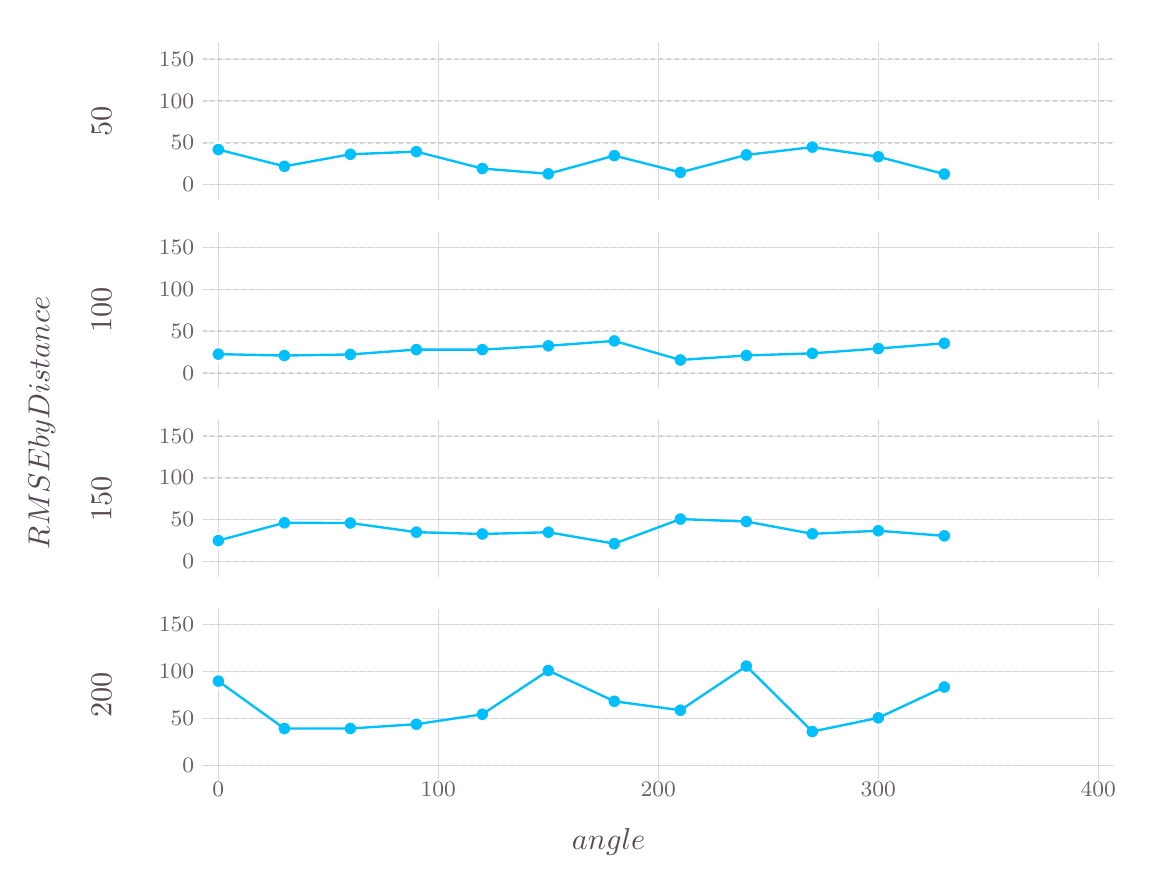
\begin{tikzpicture}[x=1mm,y=-1mm]
\definecolor{mycolor000000}{rgb}{0,0,0}
\definecolor{mycolorD0D0E0}{rgb}{0.82,0.82,0.88}
\definecolor{mycolor564A55}{rgb}{0.34,0.29,0.33}
\definecolor{mycolor6C606B}{rgb}{0.42,0.38,0.42}
\definecolor{mycolor00BFFF}{rgb}{0,0.75,1}
\definecolor{mycolor000000}{rgb}{0,0,0}
\definecolor{mycolorFFFFFF}{rgb}{1,1,1}
\begin{scope}
\begin{scope}
\draw (78.81,108.39) node [text=mycolor564A55,draw=mycolor000000,draw opacity=0,rotate around={-0: (0,1.81)},inner sep=0.0]{\fontsize{3.88mm}{4.66mm}\selectfont $\text{angle}$};
\end{scope}
\begin{scope}
\clip  (12.61,5) -- (145,5) -- (145,105.39) -- (12.61,105.39);
\begin{scope}
\clip  (12.61,5) -- (145,5) -- (145,105.39) -- (12.61,105.39);
\begin{scope}
\clip  (12.61,5) -- (145,5) -- (145,105.39) -- (12.61,105.39);
\draw (29.24,101.72) node [text=mycolor6C606B,rotate around={-0: (55.88,1.34)},inner sep=0.0]{\fontsize{2.82mm}{3.39mm}\selectfont $\text{0}$};
\draw (57.18,101.72) node [text=mycolor6C606B,rotate around={-0: (27.94,1.34)},inner sep=0.0]{\fontsize{2.82mm}{3.39mm}\selectfont $\text{100}$};
\draw (85.12,101.72) node [text=mycolor6C606B,rotate around={-0: (0,1.34)},inner sep=0.0]{\fontsize{2.82mm}{3.39mm}\selectfont $\text{200}$};
\draw (113.06,101.72) node [text=mycolor6C606B,rotate around={-0: (-27.94,1.34)},inner sep=0.0]{\fontsize{2.82mm}{3.39mm}\selectfont $\text{300}$};
\draw (141,101.72) node [text=mycolor6C606B,rotate around={-0: (-55.88,1.34)},inner sep=0.0]{\fontsize{2.82mm}{3.39mm}\selectfont $\text{400}$};
\end{scope}
\begin{scope}
\clip  (27.24,78.79) -- (143,78.79) -- (143,100.72) -- (27.24,100.72);
\begin{scope}
\clip  (27.24,78.79) -- (143,78.79) -- (143,100.72) -- (27.24,100.72);
\path [fill=mycolor000000,fill opacity=0,draw=mycolor000000,draw opacity=0] (27.24,78.79) rectangle +(115.76,21.93);
\end{scope}
\begin{scope}
[dash pattern=on 0.5mm off 0.5mm,line width=0.2mm]
\path [fill=mycolor000000,draw=mycolorD0D0E0]  (27.24,98.72) -- (143,98.72);
\path [fill=mycolor000000,draw=mycolorD0D0E0]  (27.24,92.74) -- (143,92.74);
\path [fill=mycolor000000,draw=mycolorD0D0E0]  (27.24,86.76) -- (143,86.76);
\path [fill=mycolor000000,draw=mycolorD0D0E0]  (27.24,80.79) -- (143,80.79);
\end{scope}
\begin{scope}
[dash pattern=on 0.5mm off 0.5mm,line width=0.2mm]
\path [fill=mycolor000000,draw=mycolorD0D0E0]  (29.24,78.79) -- (29.24,100.72);
\path [fill=mycolor000000,draw=mycolorD0D0E0]  (57.18,78.79) -- (57.18,100.72);
\path [fill=mycolor000000,draw=mycolorD0D0E0]  (85.12,78.79) -- (85.12,100.72);
\path [fill=mycolor000000,draw=mycolorD0D0E0]  (113.06,78.79) -- (113.06,100.72);
\path [fill=mycolor000000,draw=mycolorD0D0E0]  (141,78.79) -- (141,100.72);
\end{scope}
\begin{scope}
\begin{scope}
\begin{scope}
[line width=0.3mm]
\path [fill=mycolor00BFFF,draw=mycolorFFFFFF] (29.24,87.99) circle [radius=0.9];
\path [fill=mycolor00BFFF,draw=mycolorFFFFFF] (37.63,94.01) circle [radius=0.9];
\path [fill=mycolor00BFFF,draw=mycolorFFFFFF] (46.01,94) circle [radius=0.9];
\path [fill=mycolor00BFFF,draw=mycolorFFFFFF] (54.39,93.46) circle [radius=0.9];
\path [fill=mycolor00BFFF,draw=mycolorFFFFFF] (62.77,92.2) circle [radius=0.9];
\path [fill=mycolor00BFFF,draw=mycolorFFFFFF] (71.15,86.64) circle [radius=0.9];
\path [fill=mycolor00BFFF,draw=mycolorFFFFFF] (79.53,90.55) circle [radius=0.9];
\path [fill=mycolor00BFFF,draw=mycolorFFFFFF] (87.92,91.68) circle [radius=0.9];
\path [fill=mycolor00BFFF,draw=mycolorFFFFFF] (96.3,86.08) circle [radius=0.9];
\path [fill=mycolor00BFFF,draw=mycolorFFFFFF] (104.68,94.39) circle [radius=0.9];
\path [fill=mycolor00BFFF,draw=mycolorFFFFFF] (113.06,92.65) circle [radius=0.9];
\path [fill=mycolor00BFFF,draw=mycolorFFFFFF] (121.44,88.74) circle [radius=0.9];
\end{scope}
\end{scope}
\begin{scope}
[line width=0.3mm]
\path [fill=mycolor000000,fill opacity=0,draw=mycolor00BFFF]  (29.24,87.99) -- (37.63,94.01) -- (46.01,94) -- (54.39,93.46) -- (62.77,92.2) -- (71.15,86.64) -- (79.53,90.55) -- (87.92,91.68) -- (96.3,86.08) -- (104.68,94.39) -- (113.06,92.65) -- (121.44,88.74);
\end{scope}
\end{scope}
\end{scope}
\begin{scope}
\draw (26.24,98.72) node [text=mycolor6C606B,rotate around={-0: (-2.51,-8.96)},left,inner sep=0.0]{\fontsize{2.82mm}{3.39mm}\selectfont $\text{0}$};
\draw (26.24,92.74) node [text=mycolor6C606B,rotate around={-0: (-2.51,-2.99)},left,inner sep=0.0]{\fontsize{2.82mm}{3.39mm}\selectfont $\text{50}$};
\draw (26.24,86.76) node [text=mycolor6C606B,rotate around={-0: (-2.51,2.99)},left,inner sep=0.0]{\fontsize{2.82mm}{3.39mm}\selectfont $\text{100}$};
\draw (26.24,80.79) node [text=mycolor6C606B,rotate around={-0: (-2.51,8.96)},left,inner sep=0.0]{\fontsize{2.82mm}{3.39mm}\selectfont $\text{150}$};
\end{scope}
\begin{scope}
\draw (16.42,87.75) node [text=mycolor564A55,draw=mycolor000000,draw opacity=0,rotate around={90: (0,2)},inner sep=0.0]{\fontsize{3.88mm}{4.66mm}\selectfont $\text{200}$};
\end{scope}
\begin{scope}
\clip  (27.24,54.86) -- (143,54.86) -- (143,74.79) -- (27.24,74.79);
\begin{scope}
\clip  (27.24,54.86) -- (143,54.86) -- (143,74.79) -- (27.24,74.79);
\path [fill=mycolor000000,fill opacity=0,draw=mycolor000000,draw opacity=0] (27.24,54.86) rectangle +(115.76,19.93);
\end{scope}
\begin{scope}
[dash pattern=on 0.5mm off 0.5mm,line width=0.2mm]
\path [fill=mycolor000000,draw=mycolorD0D0E0]  (27.24,72.79) -- (143,72.79);
\path [fill=mycolor000000,draw=mycolorD0D0E0]  (27.24,67.48) -- (143,67.48);
\path [fill=mycolor000000,draw=mycolorD0D0E0]  (27.24,62.17) -- (143,62.17);
\path [fill=mycolor000000,draw=mycolorD0D0E0]  (27.24,56.86) -- (143,56.86);
\end{scope}
\begin{scope}
[dash pattern=on 0.5mm off 0.5mm,line width=0.2mm]
\path [fill=mycolor000000,draw=mycolorD0D0E0]  (29.24,54.86) -- (29.24,74.79);
\path [fill=mycolor000000,draw=mycolorD0D0E0]  (57.18,54.86) -- (57.18,74.79);
\path [fill=mycolor000000,draw=mycolorD0D0E0]  (85.12,54.86) -- (85.12,74.79);
\path [fill=mycolor000000,draw=mycolorD0D0E0]  (113.06,54.86) -- (113.06,74.79);
\path [fill=mycolor000000,draw=mycolorD0D0E0]  (141,54.86) -- (141,74.79);
\end{scope}
\begin{scope}
\begin{scope}
\begin{scope}
[line width=0.3mm]
\path [fill=mycolor00BFFF,draw=mycolorFFFFFF] (29.24,70.14) circle [radius=0.9];
\path [fill=mycolor00BFFF,draw=mycolorFFFFFF] (37.63,67.88) circle [radius=0.9];
\path [fill=mycolor00BFFF,draw=mycolorFFFFFF] (46.01,67.91) circle [radius=0.9];
\path [fill=mycolor00BFFF,draw=mycolorFFFFFF] (54.39,69.07) circle [radius=0.9];
\path [fill=mycolor00BFFF,draw=mycolorFFFFFF] (62.77,69.3) circle [radius=0.9];
\path [fill=mycolor00BFFF,draw=mycolorFFFFFF] (71.15,69.08) circle [radius=0.9];
\path [fill=mycolor00BFFF,draw=mycolorFFFFFF] (79.53,70.53) circle [radius=0.9];
\path [fill=mycolor00BFFF,draw=mycolorFFFFFF] (87.92,67.41) circle [radius=0.9];
\path [fill=mycolor00BFFF,draw=mycolorFFFFFF] (96.3,67.72) circle [radius=0.9];
\path [fill=mycolor00BFFF,draw=mycolorFFFFFF] (104.68,69.28) circle [radius=0.9];
\path [fill=mycolor00BFFF,draw=mycolorFFFFFF] (113.06,68.89) circle [radius=0.9];
\path [fill=mycolor00BFFF,draw=mycolorFFFFFF] (121.44,69.54) circle [radius=0.9];
\end{scope}
\end{scope}
\begin{scope}
[line width=0.3mm]
\path [fill=mycolor000000,fill opacity=0,draw=mycolor00BFFF]  (29.24,70.14) -- (37.63,67.88) -- (46.01,67.91) -- (54.39,69.07) -- (62.77,69.3) -- (71.15,69.08) -- (79.53,70.53) -- (87.92,67.41) -- (96.3,67.72) -- (104.68,69.28) -- (113.06,68.89) -- (121.44,69.54);
\end{scope}
\end{scope}
\end{scope}
\begin{scope}
\draw (26.24,72.79) node [text=mycolor6C606B,rotate around={-0: (-2.51,-7.96)},left,inner sep=0.0]{\fontsize{2.82mm}{3.39mm}\selectfont $\text{0}$};
\draw (26.24,67.48) node [text=mycolor6C606B,rotate around={-0: (-2.51,-2.65)},left,inner sep=0.0]{\fontsize{2.82mm}{3.39mm}\selectfont $\text{50}$};
\draw (26.24,62.17) node [text=mycolor6C606B,rotate around={-0: (-2.51,2.65)},left,inner sep=0.0]{\fontsize{2.82mm}{3.39mm}\selectfont $\text{100}$};
\draw (26.24,56.86) node [text=mycolor6C606B,rotate around={-0: (-2.51,7.96)},left,inner sep=0.0]{\fontsize{2.82mm}{3.39mm}\selectfont $\text{150}$};
\end{scope}
\begin{scope}
\draw (16.42,62.82) node [text=mycolor564A55,draw=mycolor000000,draw opacity=0,rotate around={90: (0,2)},inner sep=0.0]{\fontsize{3.88mm}{4.66mm}\selectfont $\text{150}$};
\end{scope}
\begin{scope}
\clip  (27.24,30.93) -- (143,30.93) -- (143,50.86) -- (27.24,50.86);
\begin{scope}
\clip  (27.24,30.93) -- (143,30.93) -- (143,50.86) -- (27.24,50.86);
\path [fill=mycolor000000,fill opacity=0,draw=mycolor000000,draw opacity=0] (27.24,30.93) rectangle +(115.76,19.93);
\end{scope}
\begin{scope}
[dash pattern=on 0.5mm off 0.5mm,line width=0.2mm]
\path [fill=mycolor000000,draw=mycolorD0D0E0]  (27.24,48.86) -- (143,48.86);
\path [fill=mycolor000000,draw=mycolorD0D0E0]  (27.24,43.55) -- (143,43.55);
\path [fill=mycolor000000,draw=mycolorD0D0E0]  (27.24,38.24) -- (143,38.24);
\path [fill=mycolor000000,draw=mycolorD0D0E0]  (27.24,32.93) -- (143,32.93);
\end{scope}
\begin{scope}
[dash pattern=on 0.5mm off 0.5mm,line width=0.2mm]
\path [fill=mycolor000000,draw=mycolorD0D0E0]  (29.24,30.93) -- (29.24,50.86);
\path [fill=mycolor000000,draw=mycolorD0D0E0]  (57.18,30.93) -- (57.18,50.86);
\path [fill=mycolor000000,draw=mycolorD0D0E0]  (85.12,30.93) -- (85.12,50.86);
\path [fill=mycolor000000,draw=mycolorD0D0E0]  (113.06,30.93) -- (113.06,50.86);
\path [fill=mycolor000000,draw=mycolorD0D0E0]  (141,30.93) -- (141,50.86);
\end{scope}
\begin{scope}
\begin{scope}
\begin{scope}
[line width=0.3mm]
\path [fill=mycolor00BFFF,draw=mycolorFFFFFF] (29.24,46.46) circle [radius=0.9];
\path [fill=mycolor00BFFF,draw=mycolorFFFFFF] (37.63,46.64) circle [radius=0.9];
\path [fill=mycolor00BFFF,draw=mycolorFFFFFF] (46.01,46.5) circle [radius=0.9];
\path [fill=mycolor00BFFF,draw=mycolorFFFFFF] (54.39,45.88) circle [radius=0.9];
\path [fill=mycolor00BFFF,draw=mycolorFFFFFF] (62.77,45.89) circle [radius=0.9];
\path [fill=mycolor00BFFF,draw=mycolorFFFFFF] (71.15,45.4) circle [radius=0.9];
\path [fill=mycolor00BFFF,draw=mycolorFFFFFF] (79.53,44.78) circle [radius=0.9];
\path [fill=mycolor00BFFF,draw=mycolorFFFFFF] (87.92,47.2) circle [radius=0.9];
\path [fill=mycolor00BFFF,draw=mycolorFFFFFF] (96.3,46.63) circle [radius=0.9];
\path [fill=mycolor00BFFF,draw=mycolorFFFFFF] (104.68,46.36) circle [radius=0.9];
\path [fill=mycolor00BFFF,draw=mycolorFFFFFF] (113.06,45.75) circle [radius=0.9];
\path [fill=mycolor00BFFF,draw=mycolorFFFFFF] (121.44,45.08) circle [radius=0.9];
\end{scope}
\end{scope}
\begin{scope}
[line width=0.3mm]
\path [fill=mycolor000000,fill opacity=0,draw=mycolor00BFFF]  (29.24,46.46) -- (37.63,46.64) -- (46.01,46.5) -- (54.39,45.88) -- (62.77,45.89) -- (71.15,45.4) -- (79.53,44.78) -- (87.92,47.2) -- (96.3,46.63) -- (104.68,46.36) -- (113.06,45.75) -- (121.44,45.08);
\end{scope}
\end{scope}
\end{scope}
\begin{scope}
\draw (26.24,48.86) node [text=mycolor6C606B,rotate around={-0: (-2.51,-7.96)},left,inner sep=0.0]{\fontsize{2.82mm}{3.39mm}\selectfont $\text{0}$};
\draw (26.24,43.55) node [text=mycolor6C606B,rotate around={-0: (-2.51,-2.65)},left,inner sep=0.0]{\fontsize{2.82mm}{3.39mm}\selectfont $\text{50}$};
\draw (26.24,38.24) node [text=mycolor6C606B,rotate around={-0: (-2.51,2.65)},left,inner sep=0.0]{\fontsize{2.82mm}{3.39mm}\selectfont $\text{100}$};
\draw (26.24,32.93) node [text=mycolor6C606B,rotate around={-0: (-2.51,7.96)},left,inner sep=0.0]{\fontsize{2.82mm}{3.39mm}\selectfont $\text{150}$};
\end{scope}
\begin{scope}
\draw (16.42,38.89) node [text=mycolor564A55,draw=mycolor000000,draw opacity=0,rotate around={90: (0,2)},inner sep=0.0]{\fontsize{3.88mm}{4.66mm}\selectfont $\text{100}$};
\end{scope}
\begin{scope}
\clip  (27.24,7) -- (143,7) -- (143,26.93) -- (27.24,26.93);
\begin{scope}
\clip  (27.24,7) -- (143,7) -- (143,26.93) -- (27.24,26.93);
\path [fill=mycolor000000,fill opacity=0,draw=mycolor000000,draw opacity=0] (27.24,7) rectangle +(115.76,19.93);
\end{scope}
\begin{scope}
[dash pattern=on 0.5mm off 0.5mm,line width=0.2mm]
\path [fill=mycolor000000,draw=mycolorD0D0E0]  (27.24,24.93) -- (143,24.93);
\path [fill=mycolor000000,draw=mycolorD0D0E0]  (27.24,19.62) -- (143,19.62);
\path [fill=mycolor000000,draw=mycolorD0D0E0]  (27.24,14.31) -- (143,14.31);
\path [fill=mycolor000000,draw=mycolorD0D0E0]  (27.24,9) -- (143,9);
\end{scope}
\begin{scope}
[dash pattern=on 0.5mm off 0.5mm,line width=0.2mm]
\path [fill=mycolor000000,draw=mycolorD0D0E0]  (29.24,7) -- (29.24,26.93);
\path [fill=mycolor000000,draw=mycolorD0D0E0]  (57.18,7) -- (57.18,26.93);
\path [fill=mycolor000000,draw=mycolorD0D0E0]  (85.12,7) -- (85.12,26.93);
\path [fill=mycolor000000,draw=mycolorD0D0E0]  (113.06,7) -- (113.06,26.93);
\path [fill=mycolor000000,draw=mycolorD0D0E0]  (141,7) -- (141,26.93);
\end{scope}
\begin{scope}
\begin{scope}
\begin{scope}
[line width=0.3mm]
\path [fill=mycolor00BFFF,draw=mycolorFFFFFF] (29.24,20.48) circle [radius=0.9];
\path [fill=mycolor00BFFF,draw=mycolorFFFFFF] (37.63,22.61) circle [radius=0.9];
\path [fill=mycolor00BFFF,draw=mycolorFFFFFF] (46.01,21.08) circle [radius=0.9];
\path [fill=mycolor00BFFF,draw=mycolorFFFFFF] (54.39,20.74) circle [radius=0.9];
\path [fill=mycolor00BFFF,draw=mycolorFFFFFF] (62.77,22.89) circle [radius=0.9];
\path [fill=mycolor00BFFF,draw=mycolorFFFFFF] (71.15,23.56) circle [radius=0.9];
\path [fill=mycolor00BFFF,draw=mycolorFFFFFF] (79.53,21.25) circle [radius=0.9];
\path [fill=mycolor00BFFF,draw=mycolorFFFFFF] (87.92,23.38) circle [radius=0.9];
\path [fill=mycolor00BFFF,draw=mycolorFFFFFF] (96.3,21.16) circle [radius=0.9];
\path [fill=mycolor00BFFF,draw=mycolorFFFFFF] (104.68,20.17) circle [radius=0.9];
\path [fill=mycolor00BFFF,draw=mycolorFFFFFF] (113.06,21.39) circle [radius=0.9];
\path [fill=mycolor00BFFF,draw=mycolorFFFFFF] (121.44,23.59) circle [radius=0.9];
\end{scope}
\end{scope}
\begin{scope}
[line width=0.3mm]
\path [fill=mycolor000000,fill opacity=0,draw=mycolor00BFFF]  (29.24,20.48) -- (37.63,22.61) -- (46.01,21.08) -- (54.39,20.74) -- (62.77,22.89) -- (71.15,23.56) -- (79.53,21.25) -- (87.92,23.38) -- (96.3,21.16) -- (104.68,20.17) -- (113.06,21.39) -- (121.44,23.59);
\end{scope}
\end{scope}
\end{scope}
\begin{scope}
\draw (26.24,24.93) node [text=mycolor6C606B,rotate around={-0: (-2.51,-7.96)},left,inner sep=0.0]{\fontsize{2.82mm}{3.39mm}\selectfont $\text{0}$};
\draw (26.24,19.62) node [text=mycolor6C606B,rotate around={-0: (-2.51,-2.65)},left,inner sep=0.0]{\fontsize{2.82mm}{3.39mm}\selectfont $\text{50}$};
\draw (26.24,14.31) node [text=mycolor6C606B,rotate around={-0: (-2.51,2.65)},left,inner sep=0.0]{\fontsize{2.82mm}{3.39mm}\selectfont $\text{100}$};
\draw (26.24,9) node [text=mycolor6C606B,rotate around={-0: (-2.51,7.96)},left,inner sep=0.0]{\fontsize{2.82mm}{3.39mm}\selectfont $\text{150}$};
\end{scope}
\begin{scope}
\draw (16.42,14.96) node [text=mycolor564A55,draw=mycolor000000,draw opacity=0,rotate around={90: (0,2)},inner sep=0.0]{\fontsize{3.88mm}{4.66mm}\selectfont $\text{50}$};
\end{scope}
\end{scope}
\end{scope}
\begin{scope}
\draw (8.81,53.19) node [text=mycolor564A55,draw=mycolor000000,draw opacity=0,rotate around={90: (0,2)},inner sep=0.0]{\fontsize{3.88mm}{4.66mm}\selectfont $\text{RMSE by Distance}$};
\end{scope}
\end{scope}
\end{tikzpicture}

%	\caption[RMSE for given angle and distance]{RMSE (cm) for given angle and distance (cm). In each diagram you see a the RMSE values for each angle at a fixed distance.}
%	\label{rms_eangle}
%\end{figure}

\begin{figure}[h]
	\centering
	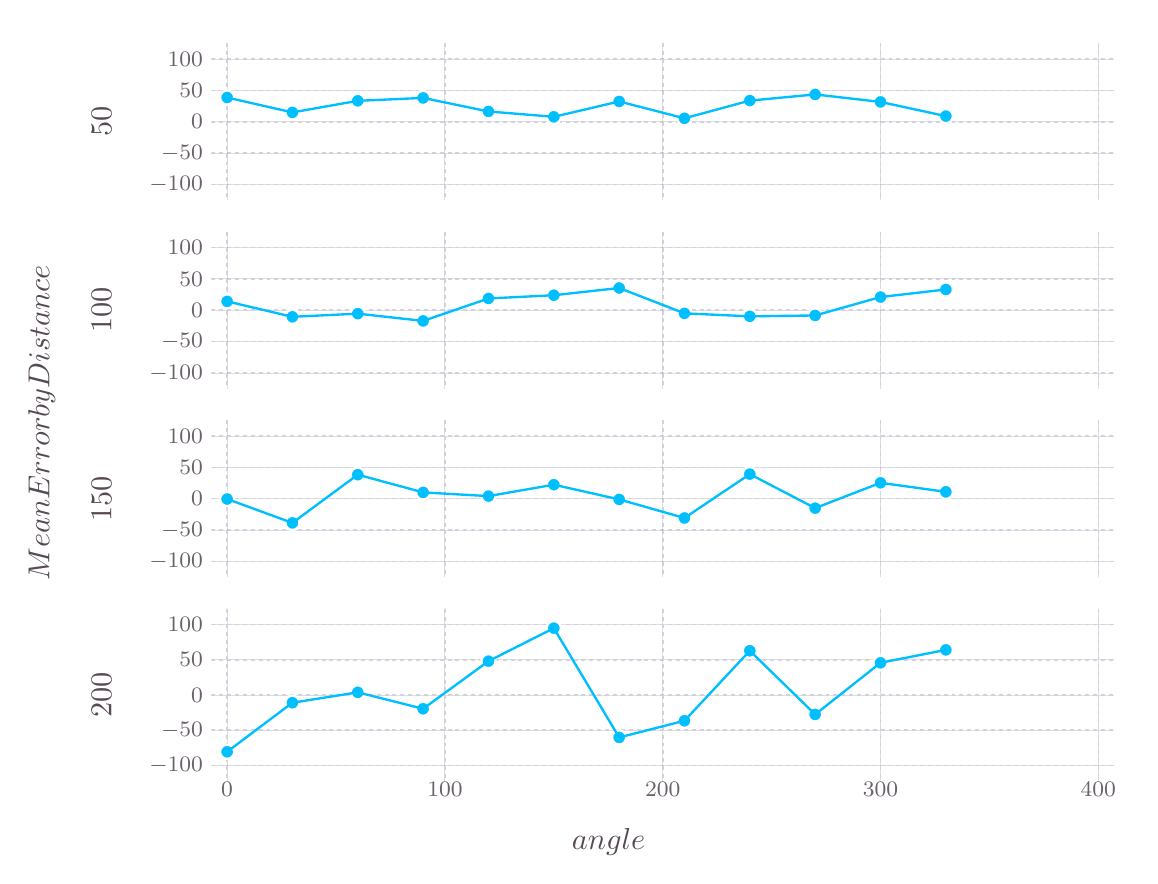
\begin{tikzpicture}[x=1mm,y=-1mm]
\definecolor{mycolor000000}{rgb}{0,0,0}
\definecolor{mycolorD0D0E0}{rgb}{0.82,0.82,0.88}
\definecolor{mycolor564A55}{rgb}{0.34,0.29,0.33}
\definecolor{mycolor6C606B}{rgb}{0.42,0.38,0.42}
\definecolor{mycolor00BFFF}{rgb}{0,0.75,1}
\definecolor{mycolor000000}{rgb}{0,0,0}
\definecolor{mycolorFFFFFF}{rgb}{1,1,1}
\begin{scope}
\begin{scope}
\draw (78.81,108.39) node [text=mycolor564A55,draw=mycolor000000,draw opacity=0,rotate around={-0: (0,1.81)},inner sep=0.0]{\fontsize{3.88mm}{4.66mm}\selectfont $\text{angle}$};
\end{scope}
\begin{scope}
\clip  (12.61,5) -- (145,5) -- (145,105.39) -- (12.61,105.39);
\begin{scope}
\clip  (12.61,5) -- (145,5) -- (145,105.39) -- (12.61,105.39);
\begin{scope}
\clip  (12.61,5) -- (145,5) -- (145,105.39) -- (12.61,105.39);
\draw (30.36,101.72) node [text=mycolor6C606B,rotate around={-0: (55.32,1.34)},inner sep=0.0]{\fontsize{2.82mm}{3.39mm}\selectfont $\text{0}$};
\draw (58.02,101.72) node [text=mycolor6C606B,rotate around={-0: (27.66,1.34)},inner sep=0.0]{\fontsize{2.82mm}{3.39mm}\selectfont $\text{100}$};
\draw (85.68,101.72) node [text=mycolor6C606B,rotate around={-0: (-0,1.34)},inner sep=0.0]{\fontsize{2.82mm}{3.39mm}\selectfont $\text{200}$};
\draw (113.34,101.72) node [text=mycolor6C606B,rotate around={-0: (-27.66,1.34)},inner sep=0.0]{\fontsize{2.82mm}{3.39mm}\selectfont $\text{300}$};
\draw (141,101.72) node [text=mycolor6C606B,rotate around={-0: (-55.32,1.34)},inner sep=0.0]{\fontsize{2.82mm}{3.39mm}\selectfont $\text{400}$};
\end{scope}
\begin{scope}
\clip  (28.36,78.79) -- (143,78.79) -- (143,100.72) -- (28.36,100.72);
\begin{scope}
\clip  (28.36,78.79) -- (143,78.79) -- (143,100.72) -- (28.36,100.72);
\path [fill=mycolor000000,fill opacity=0,draw=mycolor000000,draw opacity=0] (28.36,78.79) rectangle +(114.64,21.93);
\end{scope}
\begin{scope}
[dash pattern=on 0.5mm off 0.5mm,line width=0.2mm]
\path [fill=mycolor000000,draw=mycolorD0D0E0]  (28.36,98.72) -- (143,98.72);
\path [fill=mycolor000000,draw=mycolorD0D0E0]  (28.36,94.23) -- (143,94.23);
\path [fill=mycolor000000,draw=mycolorD0D0E0]  (28.36,89.75) -- (143,89.75);
\path [fill=mycolor000000,draw=mycolorD0D0E0]  (28.36,85.27) -- (143,85.27);
\path [fill=mycolor000000,draw=mycolorD0D0E0]  (28.36,80.79) -- (143,80.79);
\end{scope}
\begin{scope}
[dash pattern=on 0.5mm off 0.5mm,line width=0.2mm]
\path [fill=mycolor000000,draw=mycolorD0D0E0]  (30.36,78.79) -- (30.36,100.72);
\path [fill=mycolor000000,draw=mycolorD0D0E0]  (58.02,78.79) -- (58.02,100.72);
\path [fill=mycolor000000,draw=mycolorD0D0E0]  (85.68,78.79) -- (85.68,100.72);
\path [fill=mycolor000000,draw=mycolorD0D0E0]  (113.34,78.79) -- (113.34,100.72);
\path [fill=mycolor000000,draw=mycolorD0D0E0]  (141,78.79) -- (141,100.72);
\end{scope}
\begin{scope}
\begin{scope}
\begin{scope}
[line width=0.3mm]
\path [fill=mycolor00BFFF,draw=mycolorFFFFFF] (30.36,96.96) circle [radius=0.9];
\path [fill=mycolor00BFFF,draw=mycolorFFFFFF] (38.65,90.73) circle [radius=0.9];
\path [fill=mycolor00BFFF,draw=mycolorFFFFFF] (46.95,89.41) circle [radius=0.9];
\path [fill=mycolor00BFFF,draw=mycolorFFFFFF] (55.25,91.5) circle [radius=0.9];
\path [fill=mycolor00BFFF,draw=mycolorFFFFFF] (63.55,85.45) circle [radius=0.9];
\path [fill=mycolor00BFFF,draw=mycolorFFFFFF] (71.85,81.26) circle [radius=0.9];
\path [fill=mycolor00BFFF,draw=mycolorFFFFFF] (80.15,95.14) circle [radius=0.9];
\path [fill=mycolor00BFFF,draw=mycolorFFFFFF] (88.44,93.02) circle [radius=0.9];
\path [fill=mycolor00BFFF,draw=mycolorFFFFFF] (96.74,84.13) circle [radius=0.9];
\path [fill=mycolor00BFFF,draw=mycolorFFFFFF] (105.04,92.22) circle [radius=0.9];
\path [fill=mycolor00BFFF,draw=mycolorFFFFFF] (113.34,85.66) circle [radius=0.9];
\path [fill=mycolor00BFFF,draw=mycolorFFFFFF] (121.64,84.02) circle [radius=0.9];
\end{scope}
\end{scope}
\begin{scope}
[line width=0.3mm]
\path [fill=mycolor000000,fill opacity=0,draw=mycolor00BFFF]  (30.36,96.96) -- (38.65,90.73) -- (46.95,89.41) -- (55.25,91.5) -- (63.55,85.45) -- (71.85,81.26) -- (80.15,95.14) -- (88.44,93.02) -- (96.74,84.13) -- (105.04,92.22) -- (113.34,85.66) -- (121.64,84.02);
\end{scope}
\end{scope}
\end{scope}
\begin{scope}
\draw (27.36,98.72) node [text=mycolor6C606B,rotate around={-0: (-3.07,-8.96)},left,inner sep=0.0]{\fontsize{2.82mm}{3.39mm}\selectfont $\text{-100}$};
\draw (27.36,94.23) node [text=mycolor6C606B,rotate around={-0: (-3.07,-4.48)},left,inner sep=0.0]{\fontsize{2.82mm}{3.39mm}\selectfont $\text{-50}$};
\draw (27.36,89.75) node [text=mycolor6C606B,rotate around={-0: (-3.07,0)},left,inner sep=0.0]{\fontsize{2.82mm}{3.39mm}\selectfont $\text{0}$};
\draw (27.36,85.27) node [text=mycolor6C606B,rotate around={-0: (-3.07,4.48)},left,inner sep=0.0]{\fontsize{2.82mm}{3.39mm}\selectfont $\text{50}$};
\draw (27.36,80.79) node [text=mycolor6C606B,rotate around={-0: (-3.07,8.96)},left,inner sep=0.0]{\fontsize{2.82mm}{3.39mm}\selectfont $\text{100}$};
\end{scope}
\begin{scope}
\draw (16.42,87.75) node [text=mycolor564A55,draw=mycolor000000,draw opacity=0,rotate around={90: (0,2)},inner sep=0.0]{\fontsize{3.88mm}{4.66mm}\selectfont $\text{200}$};
\end{scope}
\begin{scope}
\clip  (28.36,54.86) -- (143,54.86) -- (143,74.79) -- (28.36,74.79);
\begin{scope}
\clip  (28.36,54.86) -- (143,54.86) -- (143,74.79) -- (28.36,74.79);
\path [fill=mycolor000000,fill opacity=0,draw=mycolor000000,draw opacity=0] (28.36,54.86) rectangle +(114.64,19.93);
\end{scope}
\begin{scope}
[dash pattern=on 0.5mm off 0.5mm,line width=0.2mm]
\path [fill=mycolor000000,draw=mycolorD0D0E0]  (28.36,72.79) -- (143,72.79);
\path [fill=mycolor000000,draw=mycolorD0D0E0]  (28.36,68.8) -- (143,68.8);
\path [fill=mycolor000000,draw=mycolorD0D0E0]  (28.36,64.82) -- (143,64.82);
\path [fill=mycolor000000,draw=mycolorD0D0E0]  (28.36,60.84) -- (143,60.84);
\path [fill=mycolor000000,draw=mycolorD0D0E0]  (28.36,56.86) -- (143,56.86);
\end{scope}
\begin{scope}
[dash pattern=on 0.5mm off 0.5mm,line width=0.2mm]
\path [fill=mycolor000000,draw=mycolorD0D0E0]  (30.36,54.86) -- (30.36,74.79);
\path [fill=mycolor000000,draw=mycolorD0D0E0]  (58.02,54.86) -- (58.02,74.79);
\path [fill=mycolor000000,draw=mycolorD0D0E0]  (85.68,54.86) -- (85.68,74.79);
\path [fill=mycolor000000,draw=mycolorD0D0E0]  (113.34,54.86) -- (113.34,74.79);
\path [fill=mycolor000000,draw=mycolorD0D0E0]  (141,54.86) -- (141,74.79);
\end{scope}
\begin{scope}
\begin{scope}
\begin{scope}
[line width=0.3mm]
\path [fill=mycolor00BFFF,draw=mycolorFFFFFF] (30.36,64.86) circle [radius=0.9];
\path [fill=mycolor00BFFF,draw=mycolorFFFFFF] (38.65,67.89) circle [radius=0.9];
\path [fill=mycolor00BFFF,draw=mycolorFFFFFF] (46.95,61.77) circle [radius=0.9];
\path [fill=mycolor00BFFF,draw=mycolorFFFFFF] (55.25,64.02) circle [radius=0.9];
\path [fill=mycolor00BFFF,draw=mycolorFFFFFF] (63.55,64.49) circle [radius=0.9];
\path [fill=mycolor00BFFF,draw=mycolorFFFFFF] (71.85,63.04) circle [radius=0.9];
\path [fill=mycolor00BFFF,draw=mycolorFFFFFF] (80.15,64.91) circle [radius=0.9];
\path [fill=mycolor00BFFF,draw=mycolorFFFFFF] (88.44,67.27) circle [radius=0.9];
\path [fill=mycolor00BFFF,draw=mycolorFFFFFF] (96.74,61.7) circle [radius=0.9];
\path [fill=mycolor00BFFF,draw=mycolorFFFFFF] (105.04,66.02) circle [radius=0.9];
\path [fill=mycolor00BFFF,draw=mycolorFFFFFF] (113.34,62.8) circle [radius=0.9];
\path [fill=mycolor00BFFF,draw=mycolorFFFFFF] (121.64,63.95) circle [radius=0.9];
\end{scope}
\end{scope}
\begin{scope}
[line width=0.3mm]
\path [fill=mycolor000000,fill opacity=0,draw=mycolor00BFFF]  (30.36,64.86) -- (38.65,67.89) -- (46.95,61.77) -- (55.25,64.02) -- (63.55,64.49) -- (71.85,63.04) -- (80.15,64.91) -- (88.44,67.27) -- (96.74,61.7) -- (105.04,66.02) -- (113.34,62.8) -- (121.64,63.95);
\end{scope}
\end{scope}
\end{scope}
\begin{scope}
\draw (27.36,72.79) node [text=mycolor6C606B,rotate around={-0: (-3.07,-7.96)},left,inner sep=0.0]{\fontsize{2.82mm}{3.39mm}\selectfont $\text{-100}$};
\draw (27.36,68.8) node [text=mycolor6C606B,rotate around={-0: (-3.07,-3.98)},left,inner sep=0.0]{\fontsize{2.82mm}{3.39mm}\selectfont $\text{-50}$};
\draw (27.36,64.82) node [text=mycolor6C606B,rotate around={-0: (-3.07,0)},left,inner sep=0.0]{\fontsize{2.82mm}{3.39mm}\selectfont $\text{0}$};
\draw (27.36,60.84) node [text=mycolor6C606B,rotate around={-0: (-3.07,3.98)},left,inner sep=0.0]{\fontsize{2.82mm}{3.39mm}\selectfont $\text{50}$};
\draw (27.36,56.86) node [text=mycolor6C606B,rotate around={-0: (-3.07,7.96)},left,inner sep=0.0]{\fontsize{2.82mm}{3.39mm}\selectfont $\text{100}$};
\end{scope}
\begin{scope}
\draw (16.42,62.82) node [text=mycolor564A55,draw=mycolor000000,draw opacity=0,rotate around={90: (0,2)},inner sep=0.0]{\fontsize{3.88mm}{4.66mm}\selectfont $\text{150}$};
\end{scope}
\begin{scope}
\clip  (28.36,30.93) -- (143,30.93) -- (143,50.86) -- (28.36,50.86);
\begin{scope}
\clip  (28.36,30.93) -- (143,30.93) -- (143,50.86) -- (28.36,50.86);
\path [fill=mycolor000000,fill opacity=0,draw=mycolor000000,draw opacity=0] (28.36,30.93) rectangle +(114.64,19.93);
\end{scope}
\begin{scope}
[dash pattern=on 0.5mm off 0.5mm,line width=0.2mm]
\path [fill=mycolor000000,draw=mycolorD0D0E0]  (28.36,48.86) -- (143,48.86);
\path [fill=mycolor000000,draw=mycolorD0D0E0]  (28.36,44.88) -- (143,44.88);
\path [fill=mycolor000000,draw=mycolorD0D0E0]  (28.36,40.89) -- (143,40.89);
\path [fill=mycolor000000,draw=mycolorD0D0E0]  (28.36,36.91) -- (143,36.91);
\path [fill=mycolor000000,draw=mycolorD0D0E0]  (28.36,32.93) -- (143,32.93);
\end{scope}
\begin{scope}
[dash pattern=on 0.5mm off 0.5mm,line width=0.2mm]
\path [fill=mycolor000000,draw=mycolorD0D0E0]  (30.36,30.93) -- (30.36,50.86);
\path [fill=mycolor000000,draw=mycolorD0D0E0]  (58.02,30.93) -- (58.02,50.86);
\path [fill=mycolor000000,draw=mycolorD0D0E0]  (85.68,30.93) -- (85.68,50.86);
\path [fill=mycolor000000,draw=mycolorD0D0E0]  (113.34,30.93) -- (113.34,50.86);
\path [fill=mycolor000000,draw=mycolorD0D0E0]  (141,30.93) -- (141,50.86);
\end{scope}
\begin{scope}
\begin{scope}
\begin{scope}
[line width=0.3mm]
\path [fill=mycolor00BFFF,draw=mycolorFFFFFF] (30.36,39.76) circle [radius=0.9];
\path [fill=mycolor00BFFF,draw=mycolorFFFFFF] (38.65,41.72) circle [radius=0.9];
\path [fill=mycolor00BFFF,draw=mycolorFFFFFF] (46.95,41.32) circle [radius=0.9];
\path [fill=mycolor00BFFF,draw=mycolorFFFFFF] (55.25,42.24) circle [radius=0.9];
\path [fill=mycolor00BFFF,draw=mycolorFFFFFF] (63.55,39.39) circle [radius=0.9];
\path [fill=mycolor00BFFF,draw=mycolorFFFFFF] (71.85,38.98) circle [radius=0.9];
\path [fill=mycolor00BFFF,draw=mycolorFFFFFF] (80.15,38.06) circle [radius=0.9];
\path [fill=mycolor00BFFF,draw=mycolorFFFFFF] (88.44,41.28) circle [radius=0.9];
\path [fill=mycolor00BFFF,draw=mycolorFFFFFF] (96.74,41.66) circle [radius=0.9];
\path [fill=mycolor00BFFF,draw=mycolorFFFFFF] (105.04,41.55) circle [radius=0.9];
\path [fill=mycolor00BFFF,draw=mycolorFFFFFF] (113.34,39.21) circle [radius=0.9];
\path [fill=mycolor00BFFF,draw=mycolorFFFFFF] (121.64,38.25) circle [radius=0.9];
\end{scope}
\end{scope}
\begin{scope}
[line width=0.3mm]
\path [fill=mycolor000000,fill opacity=0,draw=mycolor00BFFF]  (30.36,39.76) -- (38.65,41.72) -- (46.95,41.32) -- (55.25,42.24) -- (63.55,39.39) -- (71.85,38.98) -- (80.15,38.06) -- (88.44,41.28) -- (96.74,41.66) -- (105.04,41.55) -- (113.34,39.21) -- (121.64,38.25);
\end{scope}
\end{scope}
\end{scope}
\begin{scope}
\draw (27.36,48.86) node [text=mycolor6C606B,rotate around={-0: (-3.07,-7.96)},left,inner sep=0.0]{\fontsize{2.82mm}{3.39mm}\selectfont $\text{-100}$};
\draw (27.36,44.88) node [text=mycolor6C606B,rotate around={-0: (-3.07,-3.98)},left,inner sep=0.0]{\fontsize{2.82mm}{3.39mm}\selectfont $\text{-50}$};
\draw (27.36,40.89) node [text=mycolor6C606B,rotate around={-0: (-3.07,0)},left,inner sep=0.0]{\fontsize{2.82mm}{3.39mm}\selectfont $\text{0}$};
\draw (27.36,36.91) node [text=mycolor6C606B,rotate around={-0: (-3.07,3.98)},left,inner sep=0.0]{\fontsize{2.82mm}{3.39mm}\selectfont $\text{50}$};
\draw (27.36,32.93) node [text=mycolor6C606B,rotate around={-0: (-3.07,7.96)},left,inner sep=0.0]{\fontsize{2.82mm}{3.39mm}\selectfont $\text{100}$};
\end{scope}
\begin{scope}
\draw (16.42,38.89) node [text=mycolor564A55,draw=mycolor000000,draw opacity=0,rotate around={90: (0,2)},inner sep=0.0]{\fontsize{3.88mm}{4.66mm}\selectfont $\text{100}$};
\end{scope}
\begin{scope}
\clip  (28.36,7) -- (143,7) -- (143,26.93) -- (28.36,26.93);
\begin{scope}
\clip  (28.36,7) -- (143,7) -- (143,26.93) -- (28.36,26.93);
\path [fill=mycolor000000,fill opacity=0,draw=mycolor000000,draw opacity=0] (28.36,7) rectangle +(114.64,19.93);
\end{scope}
\begin{scope}
[dash pattern=on 0.5mm off 0.5mm,line width=0.2mm]
\path [fill=mycolor000000,draw=mycolorD0D0E0]  (28.36,24.93) -- (143,24.93);
\path [fill=mycolor000000,draw=mycolorD0D0E0]  (28.36,20.95) -- (143,20.95);
\path [fill=mycolor000000,draw=mycolorD0D0E0]  (28.36,16.96) -- (143,16.96);
\path [fill=mycolor000000,draw=mycolorD0D0E0]  (28.36,12.98) -- (143,12.98);
\path [fill=mycolor000000,draw=mycolorD0D0E0]  (28.36,9) -- (143,9);
\end{scope}
\begin{scope}
[dash pattern=on 0.5mm off 0.5mm,line width=0.2mm]
\path [fill=mycolor000000,draw=mycolorD0D0E0]  (30.36,7) -- (30.36,26.93);
\path [fill=mycolor000000,draw=mycolorD0D0E0]  (58.02,7) -- (58.02,26.93);
\path [fill=mycolor000000,draw=mycolorD0D0E0]  (85.68,7) -- (85.68,26.93);
\path [fill=mycolor000000,draw=mycolorD0D0E0]  (113.34,7) -- (113.34,26.93);
\path [fill=mycolor000000,draw=mycolorD0D0E0]  (141,7) -- (141,26.93);
\end{scope}
\begin{scope}
\begin{scope}
\begin{scope}
[line width=0.3mm]
\path [fill=mycolor00BFFF,draw=mycolorFFFFFF] (30.36,13.87) circle [radius=0.9];
\path [fill=mycolor00BFFF,draw=mycolorFFFFFF] (38.65,15.76) circle [radius=0.9];
\path [fill=mycolor00BFFF,draw=mycolorFFFFFF] (46.95,14.29) circle [radius=0.9];
\path [fill=mycolor00BFFF,draw=mycolorFFFFFF] (55.25,13.92) circle [radius=0.9];
\path [fill=mycolor00BFFF,draw=mycolorFFFFFF] (63.55,15.64) circle [radius=0.9];
\path [fill=mycolor00BFFF,draw=mycolorFFFFFF] (71.85,16.32) circle [radius=0.9];
\path [fill=mycolor00BFFF,draw=mycolorFFFFFF] (80.15,14.37) circle [radius=0.9];
\path [fill=mycolor00BFFF,draw=mycolorFFFFFF] (88.44,16.51) circle [radius=0.9];
\path [fill=mycolor00BFFF,draw=mycolorFFFFFF] (96.74,14.26) circle [radius=0.9];
\path [fill=mycolor00BFFF,draw=mycolorFFFFFF] (105.04,13.48) circle [radius=0.9];
\path [fill=mycolor00BFFF,draw=mycolorFFFFFF] (113.34,14.43) circle [radius=0.9];
\path [fill=mycolor00BFFF,draw=mycolorFFFFFF] (121.64,16.23) circle [radius=0.9];
\end{scope}
\end{scope}
\begin{scope}
[line width=0.3mm]
\path [fill=mycolor000000,fill opacity=0,draw=mycolor00BFFF]  (30.36,13.87) -- (38.65,15.76) -- (46.95,14.29) -- (55.25,13.92) -- (63.55,15.64) -- (71.85,16.32) -- (80.15,14.37) -- (88.44,16.51) -- (96.74,14.26) -- (105.04,13.48) -- (113.34,14.43) -- (121.64,16.23);
\end{scope}
\end{scope}
\end{scope}
\begin{scope}
\draw (27.36,24.93) node [text=mycolor6C606B,rotate around={-0: (-3.07,-7.96)},left,inner sep=0.0]{\fontsize{2.82mm}{3.39mm}\selectfont $\text{-100}$};
\draw (27.36,20.95) node [text=mycolor6C606B,rotate around={-0: (-3.07,-3.98)},left,inner sep=0.0]{\fontsize{2.82mm}{3.39mm}\selectfont $\text{-50}$};
\draw (27.36,16.96) node [text=mycolor6C606B,rotate around={-0: (-3.07,0)},left,inner sep=0.0]{\fontsize{2.82mm}{3.39mm}\selectfont $\text{0}$};
\draw (27.36,12.98) node [text=mycolor6C606B,rotate around={-0: (-3.07,3.98)},left,inner sep=0.0]{\fontsize{2.82mm}{3.39mm}\selectfont $\text{50}$};
\draw (27.36,9) node [text=mycolor6C606B,rotate around={-0: (-3.07,7.96)},left,inner sep=0.0]{\fontsize{2.82mm}{3.39mm}\selectfont $\text{100}$};
\end{scope}
\begin{scope}
\draw (16.42,14.96) node [text=mycolor564A55,draw=mycolor000000,draw opacity=0,rotate around={90: (0,2)},inner sep=0.0]{\fontsize{3.88mm}{4.66mm}\selectfont $\text{50}$};
\end{scope}
\end{scope}
\end{scope}
\begin{scope}
\draw (8.81,53.19) node [text=mycolor564A55,draw=mycolor000000,draw opacity=0,rotate around={90: (0,2)},inner sep=0.0]{\fontsize{3.88mm}{4.66mm}\selectfont $\text{Mean Error by Distance}$};
\end{scope}
\end{scope}
\end{tikzpicture}

	\caption[Mean Error for Given Angle]{Mean Error (cm) for Given Angle}
	\label{me_angle}
\end{figure}
\section{Properties of a Distance Function}
The ranging sensor on the FINken robot should be used to provide a distance between two quadcopters, similar to a distance measure used in swarm intelligence algorithms.

If $f(x, y)$ is a distance function it has to have the following properties.
\begin{eqnarray}
f(x, y) \ge 0 \\
f(x, y) = 0 \iff x = y \\ 
f(x, y) = f(y, x) \\ 
f(x, z) \le f(x, y) + f(y, z)
\end{eqnarray}

Of course the value measured by any real sensor will not completely accomplish to satisfy those conditions.
For use in swarm robotics it is therefore very interesting to know, in which way the range values violate the properties of a mathematical distance function.

\subsection{Non-negativity and Coincidence}

The first property of a mathematical distance measure to look at is non-negativity. This is quite easy: The values yielded by the ranging modules are positiv.
The condition for coincidence is always met as well.
Each module has a unique address and is therefore able to check if it is ranging with itself.
Having two modules occupy the same physical spot is obviously not possible, so there cannot be two different modules that are equivalent in a mathematical sense.

\subsection{Symmetry}

In this section the following notation will be used: $A \rightarrow B$ means a range reading is taken from node A with B as reflector node.

Symmetry is a property that cannot be achieved by the ranging sensors because of noise. 
A range reading $A \rightarrow B$ will not be equal to the reading for $B \rightarrow A$ just because the two readings will be altered by noise.
The remaining question is: Is the error statistically equal for both directions?

\todo{plot, evaluate, spoiler alert: Nope!}


However, the lack of symmetry might be utilised.
\begin{equation}
\frac{ d(A \rightarrow B) + d(B \rightarrow A) }{2}
\label{symavg}
\end{equation}
The remote ranging capability of the nodes can be exploited to gather both values $A \rightarrow B$ and $B \rightarrow A$ by averaging those values the error can be mitigated.

The new value showed in \autoref{symavg} will be symmetric.
Additionally, the measurement error will be reduced because of the averaging.

\subsection{Triangle Inequality}
The triangle inequality will be violated by noise.
If we measure $d(A,B) + X + d(B,C) + X$ and $d(A, C) + X$ the measurement error $X$ might cause the triangle inequality not to be met.

In \autoref{triangle} the density function for one setup of three nodes is showed.
The triangle equation is clearly violated as the \si{200}{cm} distance is underestimated by far.
This will happen a lot as there is a lot of noise especially for longer distances.
\begin{figure}[H]
	\centering
	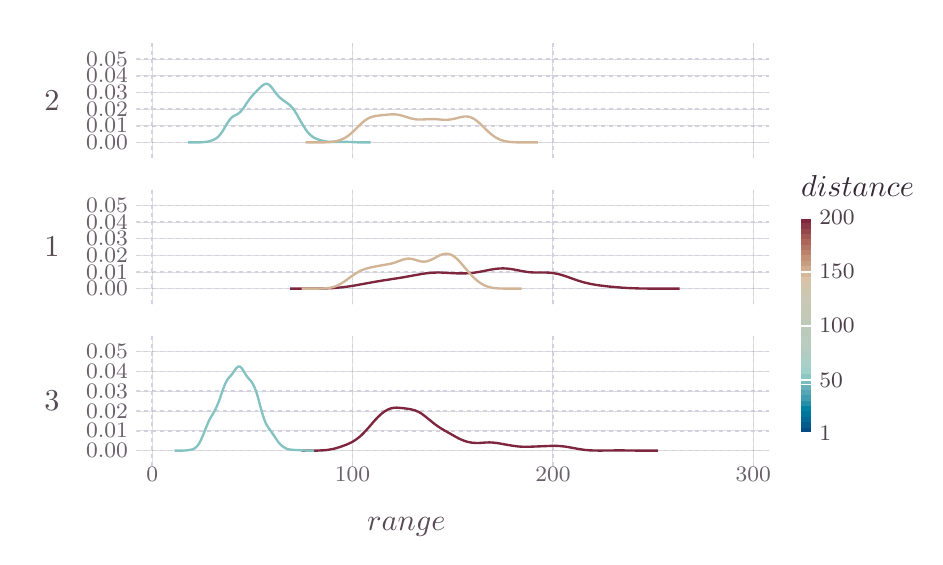
\begin{tikzpicture}[x=1mm,y=-1mm]
\definecolor{mycolor86C2C3}{rgb}{0.52,0.76,0.76}
\definecolor{mycolor409BAF}{rgb}{0.25,0.61,0.69}
\definecolor{mycolor8DC6C5}{rgb}{0.55,0.78,0.77}
\definecolor{mycolorBBCBBB}{rgb}{0.73,0.79,0.73}
\definecolor{mycolorBDCABA}{rgb}{0.74,0.79,0.73}
\definecolor{mycolor362A35}{rgb}{0.21,0.16,0.21}
\definecolor{mycolorD0D0E0}{rgb}{0.82,0.82,0.88}
\definecolor{mycolor6C606B}{rgb}{0.42,0.38,0.42}
\definecolor{mycolor7BBCC0}{rgb}{0.48,0.74,0.75}
\definecolor{mycolorB27563}{rgb}{0.7,0.46,0.39}
\definecolor{mycolor96484A}{rgb}{0.59,0.28,0.29}
\definecolor{mycolorBA836C}{rgb}{0.73,0.51,0.42}
\definecolor{mycolor000000}{rgb}{0,0,0}
\definecolor{mycolorC6C8B5}{rgb}{0.78,0.78,0.71}
\definecolor{mycolorC9C7B4}{rgb}{0.79,0.78,0.71}
\definecolor{mycolorD4C5AA}{rgb}{0.83,0.77,0.67}
\definecolor{mycolor9ED0CB}{rgb}{0.62,0.81,0.79}
\definecolor{mycolor564A55}{rgb}{0.34,0.29,0.33}
\definecolor{mycolorB5CCC1}{rgb}{0.71,0.8,0.76}
\definecolor{mycolorC2C9B7}{rgb}{0.76,0.79,0.72}
\definecolor{mycolor7E273E}{rgb}{0.49,0.15,0.24}
\definecolor{mycolorCDAB8E}{rgb}{0.81,0.67,0.56}
\definecolor{mycolor69B2BA}{rgb}{0.41,0.7,0.73}
\definecolor{mycolorC4C9B6}{rgb}{0.77,0.79,0.71}
\definecolor{mycolorC19177}{rgb}{0.76,0.57,0.47}
\definecolor{mycolorA05752}{rgb}{0.63,0.34,0.32}
\definecolor{mycolorAA665A}{rgb}{0.67,0.4,0.35}
\definecolor{mycolorB7CBBF}{rgb}{0.72,0.8,0.75}
\definecolor{mycolorBFCAB8}{rgb}{0.75,0.79,0.72}
\definecolor{mycolorC89E82}{rgb}{0.78,0.62,0.51}
\definecolor{mycolor00769D}{rgb}{0,0.46,0.61}
\definecolor{mycolor4C404B}{rgb}{0.3,0.25,0.29}
\definecolor{mycolorD2B597}{rgb}{0.82,0.71,0.59}
\definecolor{mycolor55A7B5}{rgb}{0.33,0.65,0.71}
\definecolor{mycolor7E273E}{rgb}{0.49,0.15,0.24}
\definecolor{mycolor0083A3}{rgb}{0,0.51,0.64}
\definecolor{mycolorCCC7B2}{rgb}{0.8,0.78,0.7}
\definecolor{mycolorB1CCC2}{rgb}{0.69,0.8,0.76}
\definecolor{mycolor8B3844}{rgb}{0.54,0.22,0.27}
\definecolor{mycolor005B8D}{rgb}{0,0.36,0.55}
\definecolor{mycolorABCEC4}{rgb}{0.67,0.81,0.77}
\definecolor{mycolorA5CFC7}{rgb}{0.65,0.81,0.78}
\definecolor{mycolor278FA9}{rgb}{0.15,0.56,0.66}
\definecolor{mycolorD8C3A6}{rgb}{0.85,0.76,0.65}
\definecolor{mycolor006995}{rgb}{0,0.41,0.58}
\definecolor{mycolorFFFFFF}{rgb}{1,1,1}
\definecolor{mycolorCFC6AE}{rgb}{0.81,0.78,0.68}
\definecolor{mycolorD3B79A}{rgb}{0.83,0.72,0.6}
\definecolor{mycolor004D84}{rgb}{0,0.3,0.52}
\definecolor{mycolorB9CBBD}{rgb}{0.73,0.8,0.74}
\begin{scope}
\begin{scope}
\draw (53.08,68.39) node [text=mycolor564A55,draw=mycolor000000,draw opacity=0,rotate around={-0: (0,1.81)},inner sep=0.0]{\fontsize{3.88mm}{4.66mm}\selectfont $\text{range}$};
\end{scope}
\begin{scope}
\begin{scope}
\draw (105.47,42.87) node [text=mycolor4C404B,rotate around={-0: (6.92,-0.07)},right,inner sep=0.0]{\fontsize{2.82mm}{3.39mm}\selectfont $\text{100}$};
\draw (105.47,29.15) node [text=mycolor4C404B,rotate around={-0: (6.92,13.66)},right,inner sep=0.0]{\fontsize{2.82mm}{3.39mm}\selectfont $\text{200}$};
\draw (105.47,49.74) node [text=mycolor4C404B,rotate around={-0: (6.92,-6.93)},right,inner sep=0.0]{\fontsize{2.82mm}{3.39mm}\selectfont $\text{50}$};
\draw (105.47,56.46) node [text=mycolor4C404B,rotate around={-0: (6.92,-13.66)},right,inner sep=0.0]{\fontsize{2.82mm}{3.39mm}\selectfont $\text{1}$};
\draw (105.47,36.01) node [text=mycolor4C404B,rotate around={-0: (6.92,6.79)},right,inner sep=0.0]{\fontsize{2.82mm}{3.39mm}\selectfont $\text{150}$};
\end{scope}
\begin{scope}
\path [fill=mycolor004D84,draw=mycolor000000,draw opacity=0] (103.16,55.78) rectangle +(1.31,0.68);
\path [fill=mycolor005B8D,draw=mycolor000000,draw opacity=0] (103.16,55.1) rectangle +(1.31,0.68);
\path [fill=mycolor006995,draw=mycolor000000,draw opacity=0] (103.16,54.41) rectangle +(1.31,0.68);
\path [fill=mycolor00769D,draw=mycolor000000,draw opacity=0] (103.16,53.73) rectangle +(1.31,0.68);
\path [fill=mycolor0083A3,draw=mycolor000000,draw opacity=0] (103.16,53.05) rectangle +(1.31,0.68);
\path [fill=mycolor278FA9,draw=mycolor000000,draw opacity=0] (103.16,52.36) rectangle +(1.31,0.68);
\path [fill=mycolor409BAF,draw=mycolor000000,draw opacity=0] (103.16,51.68) rectangle +(1.31,0.68);
\path [fill=mycolor55A7B5,draw=mycolor000000,draw opacity=0] (103.16,51) rectangle +(1.31,0.68);
\path [fill=mycolor69B2BA,draw=mycolor000000,draw opacity=0] (103.16,50.32) rectangle +(1.31,0.68);
\path [fill=mycolor7BBCC0,draw=mycolor000000,draw opacity=0] (103.16,49.63) rectangle +(1.31,0.68);
\path [fill=mycolor8DC6C5,draw=mycolor000000,draw opacity=0] (103.16,48.95) rectangle +(1.31,0.68);
\path [fill=mycolor9ED0CB,draw=mycolor000000,draw opacity=0] (103.16,48.27) rectangle +(1.31,0.68);
\path [fill=mycolorA5CFC7,draw=mycolor000000,draw opacity=0] (103.16,47.59) rectangle +(1.31,0.68);
\path [fill=mycolorABCEC4,draw=mycolor000000,draw opacity=0] (103.16,46.9) rectangle +(1.31,0.68);
\path [fill=mycolorB1CCC2,draw=mycolor000000,draw opacity=0] (103.16,46.22) rectangle +(1.31,0.68);
\path [fill=mycolorB5CCC1,draw=mycolor000000,draw opacity=0] (103.16,45.54) rectangle +(1.31,0.68);
\path [fill=mycolorB7CBBF,draw=mycolor000000,draw opacity=0] (103.16,44.85) rectangle +(1.31,0.68);
\path [fill=mycolorB9CBBD,draw=mycolor000000,draw opacity=0] (103.16,44.17) rectangle +(1.31,0.68);
\path [fill=mycolorBBCBBB,draw=mycolor000000,draw opacity=0] (103.16,43.49) rectangle +(1.31,0.68);
\path [fill=mycolorBDCABA,draw=mycolor000000,draw opacity=0] (103.16,42.81) rectangle +(1.31,0.68);
\path [fill=mycolorBFCAB8,draw=mycolor000000,draw opacity=0] (103.16,42.12) rectangle +(1.31,0.68);
\path [fill=mycolorC2C9B7,draw=mycolor000000,draw opacity=0] (103.16,41.44) rectangle +(1.31,0.68);
\path [fill=mycolorC4C9B6,draw=mycolor000000,draw opacity=0] (103.16,40.76) rectangle +(1.31,0.68);
\path [fill=mycolorC6C8B5,draw=mycolor000000,draw opacity=0] (103.16,40.07) rectangle +(1.31,0.68);
\path [fill=mycolorC9C7B4,draw=mycolor000000,draw opacity=0] (103.16,39.39) rectangle +(1.31,0.68);
\path [fill=mycolorCCC7B2,draw=mycolor000000,draw opacity=0] (103.16,38.71) rectangle +(1.31,0.68);
\path [fill=mycolorCFC6AE,draw=mycolor000000,draw opacity=0] (103.16,38.03) rectangle +(1.31,0.68);
\path [fill=mycolorD4C5AA,draw=mycolor000000,draw opacity=0] (103.16,37.34) rectangle +(1.31,0.68);
\path [fill=mycolorD8C3A6,draw=mycolor000000,draw opacity=0] (103.16,36.66) rectangle +(1.31,0.68);
\path [fill=mycolorD3B79A,draw=mycolor000000,draw opacity=0] (103.16,35.98) rectangle +(1.31,0.68);
\path [fill=mycolorCDAB8E,draw=mycolor000000,draw opacity=0] (103.16,35.3) rectangle +(1.31,0.68);
\path [fill=mycolorC89E82,draw=mycolor000000,draw opacity=0] (103.16,34.61) rectangle +(1.31,0.68);
\path [fill=mycolorC19177,draw=mycolor000000,draw opacity=0] (103.16,33.93) rectangle +(1.31,0.68);
\path [fill=mycolorBA836C,draw=mycolor000000,draw opacity=0] (103.16,33.25) rectangle +(1.31,0.68);
\path [fill=mycolorB27563,draw=mycolor000000,draw opacity=0] (103.16,32.56) rectangle +(1.31,0.68);
\path [fill=mycolorAA665A,draw=mycolor000000,draw opacity=0] (103.16,31.88) rectangle +(1.31,0.68);
\path [fill=mycolorA05752,draw=mycolor000000,draw opacity=0] (103.16,31.2) rectangle +(1.31,0.68);
\path [fill=mycolor96484A,draw=mycolor000000,draw opacity=0] (103.16,30.52) rectangle +(1.31,0.68);
\path [fill=mycolor8B3844,draw=mycolor000000,draw opacity=0] (103.16,29.83) rectangle +(1.31,0.68);
\path [fill=mycolor7E273E,draw=mycolor000000,draw opacity=0] (103.16,29.15) rectangle +(1.31,0.68);
\begin{scope}
[line width=0.2mm]
\path [fill=mycolor004D84,draw=mycolorFFFFFF]  (103.16,42.87) -- (104.47,42.87);
\path [fill=mycolor005B8D,draw=mycolorFFFFFF]  (103.16,29.15) -- (104.47,29.15);
\path [fill=mycolor006995,draw=mycolorFFFFFF]  (103.16,49.74) -- (104.47,49.74);
\path [fill=mycolor00769D,draw=mycolorFFFFFF]  (103.16,56.46) -- (104.47,56.46);
\path [fill=mycolor0083A3,draw=mycolorFFFFFF]  (103.16,36.01) -- (104.47,36.01);
\end{scope}
\end{scope}
\begin{scope}
\draw (103.16,25.15) node [text=mycolor362A35,draw=mycolor000000,draw opacity=0,rotate around={-0: (6.92,0.19)},right,inner sep=0.0]{\fontsize{3.88mm}{4.66mm}\selectfont $\text{distance}$};
\end{scope}
\end{scope}
\begin{scope}
\clip  (5,5) -- (101.16,5) -- (101.16,65.39) -- (5,65.39);
\begin{scope}
\clip  (5,5) -- (101.16,5) -- (101.16,65.39) -- (5,65.39);
\begin{scope}
\clip  (5,5) -- (101.16,5) -- (101.16,65.39) -- (5,65.39);
\draw (20.81,61.71) node [text=mycolor6C606B,rotate around={-0: (38.17,1.34)},inner sep=0.0]{\fontsize{2.82mm}{3.39mm}\selectfont $\text{0}$};
\draw (46.26,61.71) node [text=mycolor6C606B,rotate around={-0: (12.72,1.34)},inner sep=0.0]{\fontsize{2.82mm}{3.39mm}\selectfont $\text{100}$};
\draw (71.71,61.71) node [text=mycolor6C606B,rotate around={-0: (-12.72,1.34)},inner sep=0.0]{\fontsize{2.82mm}{3.39mm}\selectfont $\text{200}$};
\draw (97.16,61.71) node [text=mycolor6C606B,rotate around={-0: (-38.17,1.34)},inner sep=0.0]{\fontsize{2.82mm}{3.39mm}\selectfont $\text{300}$};
\end{scope}
\begin{scope}
\clip  (18.81,44.14) -- (99.16,44.14) -- (99.16,60.71) -- (18.81,60.71);
\begin{scope}
\clip  (18.81,44.14) -- (99.16,44.14) -- (99.16,60.71) -- (18.81,60.71);
\path [fill=mycolor000000,fill opacity=0,draw=mycolor000000,draw opacity=0] (18.81,44.14) rectangle +(80.35,16.57);
\end{scope}
\begin{scope}
[dash pattern=on 0.5mm off 0.5mm,line width=0.2mm]
\path [fill=mycolor000000,draw=mycolorD0D0E0]  (18.81,58.71) -- (99.16,58.71);
\path [fill=mycolor000000,draw=mycolorD0D0E0]  (18.81,56.2) -- (99.16,56.2);
\path [fill=mycolor000000,draw=mycolorD0D0E0]  (18.81,53.69) -- (99.16,53.69);
\path [fill=mycolor000000,draw=mycolorD0D0E0]  (18.81,51.17) -- (99.16,51.17);
\path [fill=mycolor000000,draw=mycolorD0D0E0]  (18.81,48.66) -- (99.16,48.66);
\path [fill=mycolor000000,draw=mycolorD0D0E0]  (18.81,46.14) -- (99.16,46.14);
\end{scope}
\begin{scope}
[dash pattern=on 0.5mm off 0.5mm,line width=0.2mm]
\path [fill=mycolor000000,draw=mycolorD0D0E0]  (20.81,44.14) -- (20.81,60.71);
\path [fill=mycolor000000,draw=mycolorD0D0E0]  (46.26,44.14) -- (46.26,60.71);
\path [fill=mycolor000000,draw=mycolorD0D0E0]  (71.71,44.14) -- (71.71,60.71);
\path [fill=mycolor000000,draw=mycolorD0D0E0]  (97.16,44.14) -- (97.16,60.71);
\end{scope}
\begin{scope}
\begin{scope}
[line width=0.3mm]
\path [fill=mycolor000000,fill opacity=0,draw=mycolor7E273E]  (39.79,58.71) -- (39.94,58.71) -- (40.09,58.71) -- (40.24,58.71) -- (40.39,58.71) -- (40.54,58.71) -- (40.7,58.71) -- (40.85,58.71) -- (41,58.71) -- (41.15,58.71) -- (41.3,58.71) -- (41.45,58.71) -- (41.6,58.71) -- (41.76,58.71) -- (41.91,58.7) -- (42.06,58.7) -- (42.21,58.69) -- (42.36,58.68) -- (42.51,58.68) -- (42.66,58.66) -- (42.82,58.65) -- (42.97,58.64) -- (43.12,58.62) -- (43.27,58.59) -- (43.42,58.57) -- (43.57,58.54) -- (43.72,58.51) -- (43.88,58.48) -- (44.03,58.44) -- (44.18,58.4) -- (44.33,58.35) -- (44.48,58.31) -- (44.63,58.26) -- (44.78,58.21) -- (44.93,58.16) -- (45.09,58.1) -- (45.24,58.05) -- (45.39,57.99) -- (45.54,57.93) -- (45.69,57.86) -- (45.84,57.8) -- (45.99,57.72) -- (46.15,57.65) -- (46.3,57.56) -- (46.45,57.47) -- (46.6,57.38) -- (46.75,57.27) -- (46.9,57.16) -- (47.05,57.04) -- (47.21,56.91) -- (47.36,56.78) -- (47.51,56.63) -- (47.66,56.48) -- (47.81,56.32) -- (47.96,56.16) -- (48.11,55.99) -- (48.27,55.82) -- (48.42,55.65) -- (48.57,55.47) -- (48.72,55.3) -- (48.87,55.12) -- (49.02,54.95) -- (49.17,54.78) -- (49.33,54.62) -- (49.48,54.46) -- (49.63,54.32) -- (49.78,54.17) -- (49.93,54.04) -- (50.08,53.92) -- (50.23,53.81) -- (50.38,53.7) -- (50.54,53.61) -- (50.69,53.53) -- (50.84,53.46) -- (50.99,53.4) -- (51.14,53.35) -- (51.29,53.32) -- (51.44,53.29) -- (51.6,53.27) -- (51.75,53.26) -- (51.9,53.26) -- (52.05,53.27) -- (52.2,53.28) -- (52.35,53.29) -- (52.5,53.31) -- (52.66,53.32) -- (52.81,53.34) -- (52.96,53.36) -- (53.11,53.38) -- (53.26,53.4) -- (53.41,53.43) -- (53.56,53.45) -- (53.72,53.48) -- (53.87,53.52) -- (54.02,53.56) -- (54.17,53.6) -- (54.32,53.66) -- (54.47,53.72) -- (54.62,53.79) -- (54.78,53.87) -- (54.93,53.96) -- (55.08,54.06) -- (55.23,54.17) -- (55.38,54.28) -- (55.53,54.4) -- (55.68,54.52) -- (55.83,54.64) -- (55.99,54.77) -- (56.14,54.89) -- (56.29,55.02) -- (56.44,55.14) -- (56.59,55.26) -- (56.74,55.37) -- (56.89,55.48) -- (57.05,55.59) -- (57.2,55.69) -- (57.35,55.79) -- (57.5,55.89) -- (57.65,55.98) -- (57.8,56.07) -- (57.95,56.16) -- (58.11,56.24) -- (58.26,56.33) -- (58.41,56.42) -- (58.56,56.5) -- (58.71,56.59) -- (58.86,56.68) -- (59.01,56.76) -- (59.17,56.85) -- (59.32,56.94) -- (59.47,57.02) -- (59.62,57.1) -- (59.77,57.18) -- (59.92,57.25) -- (60.07,57.32) -- (60.23,57.38) -- (60.38,57.44) -- (60.53,57.49) -- (60.68,57.54) -- (60.83,57.59) -- (60.98,57.62) -- (61.13,57.66) -- (61.28,57.68) -- (61.44,57.71) -- (61.59,57.72) -- (61.74,57.73) -- (61.89,57.74) -- (62.04,57.74) -- (62.19,57.74) -- (62.34,57.74) -- (62.5,57.73) -- (62.65,57.72) -- (62.8,57.71) -- (62.95,57.7) -- (63.1,57.69) -- (63.25,57.68) -- (63.4,57.68) -- (63.56,57.67) -- (63.71,57.67) -- (63.86,57.68) -- (64.01,57.69) -- (64.16,57.7) -- (64.31,57.72) -- (64.46,57.73) -- (64.62,57.75) -- (64.77,57.78) -- (64.92,57.8) -- (65.07,57.83) -- (65.22,57.86) -- (65.37,57.88) -- (65.52,57.91) -- (65.68,57.94) -- (65.83,57.96) -- (65.98,57.99) -- (66.13,58.02) -- (66.28,58.04) -- (66.43,58.07) -- (66.58,58.09) -- (66.73,58.11) -- (66.89,58.13) -- (67.04,58.15) -- (67.19,58.17) -- (67.34,58.19) -- (67.49,58.2) -- (67.64,58.21) -- (67.79,58.22) -- (67.95,58.23) -- (68.1,58.23) -- (68.25,58.23) -- (68.4,58.23) -- (68.55,58.23) -- (68.7,58.22) -- (68.85,58.22) -- (69.01,58.21) -- (69.16,58.21) -- (69.31,58.2) -- (69.46,58.19) -- (69.61,58.19) -- (69.76,58.18) -- (69.91,58.17) -- (70.07,58.17) -- (70.22,58.16) -- (70.37,58.16) -- (70.52,58.15) -- (70.67,58.14) -- (70.82,58.14) -- (70.97,58.13) -- (71.13,58.12) -- (71.28,58.12) -- (71.43,58.11) -- (71.58,58.11) -- (71.73,58.1) -- (71.88,58.1) -- (72.03,58.11) -- (72.18,58.11) -- (72.34,58.12) -- (72.49,58.12) -- (72.64,58.14) -- (72.79,58.15) -- (72.94,58.17) -- (73.09,58.18) -- (73.24,58.2) -- (73.4,58.23) -- (73.55,58.25) -- (73.7,58.27) -- (73.85,58.3) -- (74,58.33) -- (74.15,58.36) -- (74.3,58.38) -- (74.46,58.41) -- (74.61,58.44) -- (74.76,58.47) -- (74.91,58.49) -- (75.06,58.52) -- (75.21,58.54) -- (75.36,58.57) -- (75.52,58.59) -- (75.67,58.61) -- (75.82,58.63) -- (75.97,58.64) -- (76.12,58.65) -- (76.27,58.67) -- (76.42,58.68) -- (76.58,58.68) -- (76.73,58.69) -- (76.88,58.7) -- (77.03,58.7) -- (77.18,58.7) -- (77.33,58.7) -- (77.48,58.71) -- (77.63,58.71) -- (77.79,58.71) -- (77.94,58.71) -- (78.09,58.7) -- (78.24,58.7) -- (78.39,58.7) -- (78.54,58.7) -- (78.69,58.7) -- (78.85,58.69) -- (79,58.69) -- (79.15,58.69) -- (79.3,58.69) -- (79.45,58.69) -- (79.6,58.68) -- (79.75,58.68) -- (79.91,58.68) -- (80.06,58.68) -- (80.21,58.68) -- (80.36,58.68) -- (80.51,58.68) -- (80.66,58.68) -- (80.81,58.69) -- (80.97,58.69) -- (81.12,58.69) -- (81.27,58.69) -- (81.42,58.7) -- (81.57,58.7) -- (81.72,58.7) -- (81.87,58.7) -- (82.03,58.7) -- (82.18,58.71) -- (82.33,58.71) -- (82.48,58.71) -- (82.63,58.71) -- (82.78,58.71) -- (82.93,58.71) -- (83.08,58.71) -- (83.24,58.71) -- (83.39,58.71) -- (83.54,58.71) -- (83.69,58.71) -- (83.84,58.71) -- (83.99,58.71) -- (84.14,58.71) -- (84.3,58.71) -- (84.45,58.71) -- (84.6,58.71) -- (84.75,58.71) -- (84.9,58.71) -- (85.05,58.71);
\path [fill=mycolor000000,fill opacity=0,draw=mycolor86C2C3]  (23.66,58.71) -- (23.72,58.71) -- (23.78,58.71) -- (23.83,58.71) -- (23.89,58.71) -- (23.95,58.71) -- (24.01,58.71) -- (24.07,58.71) -- (24.13,58.71) -- (24.19,58.71) -- (24.25,58.71) -- (24.31,58.71) -- (24.37,58.71) -- (24.43,58.71) -- (24.49,58.71) -- (24.55,58.71) -- (24.6,58.71) -- (24.66,58.71) -- (24.72,58.71) -- (24.78,58.7) -- (24.84,58.7) -- (24.9,58.7) -- (24.96,58.7) -- (25.02,58.69) -- (25.08,58.69) -- (25.14,58.68) -- (25.2,58.68) -- (25.26,58.67) -- (25.32,58.66) -- (25.38,58.66) -- (25.43,58.65) -- (25.49,58.64) -- (25.55,58.63) -- (25.61,58.62) -- (25.67,58.61) -- (25.73,58.6) -- (25.79,58.59) -- (25.85,58.57) -- (25.91,58.55) -- (25.97,58.53) -- (26.03,58.51) -- (26.09,58.48) -- (26.15,58.45) -- (26.21,58.42) -- (26.26,58.38) -- (26.32,58.33) -- (26.38,58.28) -- (26.44,58.23) -- (26.5,58.16) -- (26.56,58.09) -- (26.62,58.02) -- (26.68,57.94) -- (26.74,57.85) -- (26.8,57.75) -- (26.86,57.65) -- (26.92,57.53) -- (26.98,57.42) -- (27.04,57.29) -- (27.09,57.17) -- (27.15,57.03) -- (27.21,56.89) -- (27.27,56.75) -- (27.33,56.6) -- (27.39,56.46) -- (27.45,56.3) -- (27.51,56.15) -- (27.57,56) -- (27.63,55.85) -- (27.69,55.7) -- (27.75,55.56) -- (27.81,55.42) -- (27.86,55.28) -- (27.92,55.15) -- (27.98,55.02) -- (28.04,54.9) -- (28.1,54.78) -- (28.16,54.66) -- (28.22,54.56) -- (28.28,54.45) -- (28.34,54.35) -- (28.4,54.25) -- (28.46,54.15) -- (28.52,54.05) -- (28.58,53.95) -- (28.64,53.85) -- (28.69,53.75) -- (28.75,53.64) -- (28.81,53.53) -- (28.87,53.41) -- (28.93,53.29) -- (28.99,53.16) -- (29.05,53.03) -- (29.11,52.89) -- (29.17,52.74) -- (29.23,52.59) -- (29.29,52.43) -- (29.35,52.27) -- (29.41,52.11) -- (29.47,51.94) -- (29.52,51.77) -- (29.58,51.59) -- (29.64,51.42) -- (29.7,51.25) -- (29.76,51.08) -- (29.82,50.91) -- (29.88,50.75) -- (29.94,50.59) -- (30,50.44) -- (30.06,50.3) -- (30.12,50.17) -- (30.18,50.04) -- (30.24,49.93) -- (30.29,49.82) -- (30.35,49.73) -- (30.41,49.64) -- (30.47,49.56) -- (30.53,49.49) -- (30.59,49.42) -- (30.65,49.35) -- (30.71,49.29) -- (30.77,49.22) -- (30.83,49.15) -- (30.89,49.08) -- (30.95,49.01) -- (31.01,48.93) -- (31.07,48.85) -- (31.12,48.77) -- (31.18,48.68) -- (31.24,48.59) -- (31.3,48.51) -- (31.36,48.42) -- (31.42,48.34) -- (31.48,48.27) -- (31.54,48.2) -- (31.6,48.14) -- (31.66,48.09) -- (31.72,48.05) -- (31.78,48.03) -- (31.84,48.02) -- (31.9,48.03) -- (31.95,48.05) -- (32.01,48.08) -- (32.07,48.13) -- (32.13,48.19) -- (32.19,48.26) -- (32.25,48.34) -- (32.31,48.42) -- (32.37,48.52) -- (32.43,48.61) -- (32.49,48.71) -- (32.55,48.81) -- (32.61,48.91) -- (32.67,49.01) -- (32.72,49.1) -- (32.78,49.19) -- (32.84,49.27) -- (32.9,49.35) -- (32.96,49.43) -- (33.02,49.5) -- (33.08,49.57) -- (33.14,49.64) -- (33.2,49.7) -- (33.26,49.77) -- (33.32,49.84) -- (33.38,49.91) -- (33.44,49.99) -- (33.5,50.08) -- (33.55,50.17) -- (33.61,50.27) -- (33.67,50.38) -- (33.73,50.5) -- (33.79,50.63) -- (33.85,50.77) -- (33.91,50.92) -- (33.97,51.09) -- (34.03,51.26) -- (34.09,51.44) -- (34.15,51.63) -- (34.21,51.83) -- (34.27,52.04) -- (34.33,52.25) -- (34.38,52.47) -- (34.44,52.69) -- (34.5,52.91) -- (34.56,53.13) -- (34.62,53.35) -- (34.68,53.57) -- (34.74,53.78) -- (34.8,53.98) -- (34.86,54.18) -- (34.92,54.37) -- (34.98,54.55) -- (35.04,54.72) -- (35.1,54.87) -- (35.15,55.02) -- (35.21,55.16) -- (35.27,55.28) -- (35.33,55.4) -- (35.39,55.51) -- (35.45,55.61) -- (35.51,55.71) -- (35.57,55.8) -- (35.63,55.88) -- (35.69,55.97) -- (35.75,56.05) -- (35.81,56.13) -- (35.87,56.21) -- (35.93,56.3) -- (35.98,56.38) -- (36.04,56.46) -- (36.1,56.55) -- (36.16,56.64) -- (36.22,56.72) -- (36.28,56.81) -- (36.34,56.9) -- (36.4,56.99) -- (36.46,57.08) -- (36.52,57.17) -- (36.58,57.26) -- (36.64,57.34) -- (36.7,57.43) -- (36.76,57.51) -- (36.81,57.59) -- (36.87,57.67) -- (36.93,57.74) -- (36.99,57.81) -- (37.05,57.88) -- (37.11,57.94) -- (37.17,58) -- (37.23,58.06) -- (37.29,58.11) -- (37.35,58.16) -- (37.41,58.2) -- (37.47,58.24) -- (37.53,58.28) -- (37.59,58.32) -- (37.64,58.35) -- (37.7,58.38) -- (37.76,58.41) -- (37.82,58.43) -- (37.88,58.46) -- (37.94,58.48) -- (38,58.5) -- (38.06,58.52) -- (38.12,58.53) -- (38.18,58.55) -- (38.24,58.56) -- (38.3,58.57) -- (38.36,58.58) -- (38.41,58.59) -- (38.47,58.6) -- (38.53,58.61) -- (38.59,58.61) -- (38.65,58.62) -- (38.71,58.62) -- (38.77,58.62) -- (38.83,58.62) -- (38.89,58.63) -- (38.95,58.63) -- (39.01,58.63) -- (39.07,58.63) -- (39.13,58.63) -- (39.19,58.63) -- (39.24,58.64) -- (39.3,58.64) -- (39.36,58.64) -- (39.42,58.65) -- (39.48,58.65) -- (39.54,58.66) -- (39.6,58.66) -- (39.66,58.67) -- (39.72,58.67) -- (39.78,58.68) -- (39.84,58.68) -- (39.9,58.68) -- (39.96,58.69) -- (40.02,58.69) -- (40.07,58.7) -- (40.13,58.7) -- (40.19,58.7) -- (40.25,58.7) -- (40.31,58.71) -- (40.37,58.71) -- (40.43,58.71) -- (40.49,58.71) -- (40.55,58.71) -- (40.61,58.71) -- (40.67,58.71) -- (40.73,58.71) -- (40.79,58.71) -- (40.84,58.71) -- (40.9,58.71) -- (40.96,58.71) -- (41.02,58.71) -- (41.08,58.71) -- (41.14,58.71) -- (41.2,58.71) -- (41.26,58.71) -- (41.32,58.71) -- (41.38,58.71);
\end{scope}
\end{scope}
\end{scope}
\begin{scope}
\draw (17.81,58.71) node [text=mycolor6C606B,rotate around={-0: (-2.85,-6.29)},left,inner sep=0.0]{\fontsize{2.82mm}{3.39mm}\selectfont $\text{0.00}$};
\draw (17.81,56.2) node [text=mycolor6C606B,rotate around={-0: (-2.85,-3.77)},left,inner sep=0.0]{\fontsize{2.82mm}{3.39mm}\selectfont $\text{0.01}$};
\draw (17.81,53.69) node [text=mycolor6C606B,rotate around={-0: (-2.85,-1.26)},left,inner sep=0.0]{\fontsize{2.82mm}{3.39mm}\selectfont $\text{0.02}$};
\draw (17.81,51.17) node [text=mycolor6C606B,rotate around={-0: (-2.85,1.26)},left,inner sep=0.0]{\fontsize{2.82mm}{3.39mm}\selectfont $\text{0.03}$};
\draw (17.81,48.66) node [text=mycolor6C606B,rotate around={-0: (-2.85,3.77)},left,inner sep=0.0]{\fontsize{2.82mm}{3.39mm}\selectfont $\text{0.04}$};
\draw (17.81,46.14) node [text=mycolor6C606B,rotate around={-0: (-2.85,6.29)},left,inner sep=0.0]{\fontsize{2.82mm}{3.39mm}\selectfont $\text{0.05}$};
\end{scope}
\begin{scope}
\draw (9.12,52.43) node [text=mycolor564A55,draw=mycolor000000,draw opacity=0,rotate around={-0: (-1.06,0)},left,inner sep=0.0]{\fontsize{3.88mm}{4.66mm}\selectfont $\text{3}$};
\end{scope}
\begin{scope}
\clip  (18.81,25.57) -- (99.16,25.57) -- (99.16,40.14) -- (18.81,40.14);
\begin{scope}
\clip  (18.81,25.57) -- (99.16,25.57) -- (99.16,40.14) -- (18.81,40.14);
\path [fill=mycolor000000,fill opacity=0,draw=mycolor000000,draw opacity=0] (18.81,25.57) rectangle +(80.35,14.57);
\end{scope}
\begin{scope}
[dash pattern=on 0.5mm off 0.5mm,line width=0.2mm]
\path [fill=mycolor000000,draw=mycolorD0D0E0]  (18.81,38.14) -- (99.16,38.14);
\path [fill=mycolor000000,draw=mycolorD0D0E0]  (18.81,36.03) -- (99.16,36.03);
\path [fill=mycolor000000,draw=mycolorD0D0E0]  (18.81,33.91) -- (99.16,33.91);
\path [fill=mycolor000000,draw=mycolorD0D0E0]  (18.81,31.8) -- (99.16,31.8);
\path [fill=mycolor000000,draw=mycolorD0D0E0]  (18.81,29.69) -- (99.16,29.69);
\path [fill=mycolor000000,draw=mycolorD0D0E0]  (18.81,27.57) -- (99.16,27.57);
\end{scope}
\begin{scope}
[dash pattern=on 0.5mm off 0.5mm,line width=0.2mm]
\path [fill=mycolor000000,draw=mycolorD0D0E0]  (20.81,25.57) -- (20.81,40.14);
\path [fill=mycolor000000,draw=mycolorD0D0E0]  (46.26,25.57) -- (46.26,40.14);
\path [fill=mycolor000000,draw=mycolorD0D0E0]  (71.71,25.57) -- (71.71,40.14);
\path [fill=mycolor000000,draw=mycolorD0D0E0]  (97.16,25.57) -- (97.16,40.14);
\end{scope}
\begin{scope}
\begin{scope}
[line width=0.3mm]
\path [fill=mycolor000000,fill opacity=0,draw=mycolor7E273E]  (38.32,38.14) -- (38.49,38.14) -- (38.65,38.14) -- (38.82,38.14) -- (38.98,38.14) -- (39.15,38.14) -- (39.31,38.14) -- (39.48,38.14) -- (39.64,38.14) -- (39.81,38.14) -- (39.97,38.14) -- (40.14,38.14) -- (40.31,38.14) -- (40.47,38.14) -- (40.64,38.14) -- (40.8,38.14) -- (40.97,38.14) -- (41.13,38.14) -- (41.3,38.14) -- (41.46,38.14) -- (41.63,38.14) -- (41.79,38.13) -- (41.96,38.13) -- (42.13,38.13) -- (42.29,38.13) -- (42.46,38.12) -- (42.62,38.12) -- (42.79,38.11) -- (42.95,38.11) -- (43.12,38.1) -- (43.28,38.1) -- (43.45,38.09) -- (43.61,38.08) -- (43.78,38.07) -- (43.95,38.06) -- (44.11,38.05) -- (44.28,38.03) -- (44.44,38.02) -- (44.61,38) -- (44.77,37.99) -- (44.94,37.97) -- (45.1,37.95) -- (45.27,37.93) -- (45.43,37.91) -- (45.6,37.89) -- (45.77,37.86) -- (45.93,37.84) -- (46.1,37.81) -- (46.26,37.79) -- (46.43,37.76) -- (46.59,37.73) -- (46.76,37.7) -- (46.92,37.67) -- (47.09,37.64) -- (47.25,37.61) -- (47.42,37.58) -- (47.59,37.55) -- (47.75,37.52) -- (47.92,37.49) -- (48.08,37.46) -- (48.25,37.43) -- (48.41,37.4) -- (48.58,37.37) -- (48.74,37.34) -- (48.91,37.31) -- (49.07,37.28) -- (49.24,37.25) -- (49.41,37.22) -- (49.57,37.2) -- (49.74,37.17) -- (49.9,37.14) -- (50.07,37.11) -- (50.23,37.09) -- (50.4,37.06) -- (50.56,37.04) -- (50.73,37.01) -- (50.89,36.99) -- (51.06,36.96) -- (51.23,36.93) -- (51.39,36.91) -- (51.56,36.88) -- (51.72,36.86) -- (51.89,36.83) -- (52.05,36.81) -- (52.22,36.78) -- (52.38,36.75) -- (52.55,36.73) -- (52.71,36.7) -- (52.88,36.67) -- (53.05,36.64) -- (53.21,36.61) -- (53.38,36.58) -- (53.54,36.55) -- (53.71,36.52) -- (53.87,36.49) -- (54.04,36.46) -- (54.2,36.43) -- (54.37,36.4) -- (54.54,36.37) -- (54.7,36.34) -- (54.87,36.31) -- (55.03,36.28) -- (55.2,36.26) -- (55.36,36.23) -- (55.53,36.21) -- (55.69,36.19) -- (55.86,36.17) -- (56.02,36.15) -- (56.19,36.14) -- (56.36,36.12) -- (56.52,36.11) -- (56.69,36.11) -- (56.85,36.1) -- (57.02,36.1) -- (57.18,36.1) -- (57.35,36.1) -- (57.51,36.1) -- (57.68,36.11) -- (57.84,36.12) -- (58.01,36.12) -- (58.18,36.13) -- (58.34,36.14) -- (58.51,36.15) -- (58.67,36.16) -- (58.84,36.17) -- (59,36.18) -- (59.17,36.19) -- (59.33,36.19) -- (59.5,36.2) -- (59.66,36.21) -- (59.83,36.21) -- (60,36.21) -- (60.16,36.21) -- (60.33,36.21) -- (60.49,36.21) -- (60.66,36.2) -- (60.82,36.19) -- (60.99,36.18) -- (61.15,36.17) -- (61.32,36.16) -- (61.48,36.14) -- (61.65,36.12) -- (61.82,36.1) -- (61.98,36.07) -- (62.15,36.05) -- (62.31,36.02) -- (62.48,35.99) -- (62.64,35.96) -- (62.81,35.93) -- (62.97,35.9) -- (63.14,35.86) -- (63.3,35.83) -- (63.47,35.8) -- (63.64,35.76) -- (63.8,35.73) -- (63.97,35.7) -- (64.13,35.68) -- (64.3,35.65) -- (64.46,35.63) -- (64.63,35.61) -- (64.79,35.6) -- (64.96,35.58) -- (65.12,35.58) -- (65.29,35.57) -- (65.46,35.57) -- (65.62,35.58) -- (65.79,35.59) -- (65.95,35.6) -- (66.12,35.62) -- (66.28,35.64) -- (66.45,35.66) -- (66.61,35.69) -- (66.78,35.72) -- (66.94,35.75) -- (67.11,35.78) -- (67.28,35.81) -- (67.44,35.85) -- (67.61,35.88) -- (67.77,35.91) -- (67.94,35.94) -- (68.1,35.97) -- (68.27,35.99) -- (68.43,36.02) -- (68.6,36.04) -- (68.76,36.05) -- (68.93,36.07) -- (69.1,36.08) -- (69.26,36.09) -- (69.43,36.09) -- (69.59,36.09) -- (69.76,36.1) -- (69.92,36.1) -- (70.09,36.1) -- (70.25,36.09) -- (70.42,36.09) -- (70.59,36.1) -- (70.75,36.1) -- (70.92,36.1) -- (71.08,36.11) -- (71.25,36.12) -- (71.41,36.13) -- (71.58,36.15) -- (71.74,36.17) -- (71.91,36.2) -- (72.07,36.23) -- (72.24,36.26) -- (72.41,36.3) -- (72.57,36.34) -- (72.74,36.38) -- (72.9,36.43) -- (73.07,36.48) -- (73.23,36.54) -- (73.4,36.59) -- (73.56,36.65) -- (73.73,36.71) -- (73.89,36.77) -- (74.06,36.83) -- (74.23,36.89) -- (74.39,36.95) -- (74.56,37) -- (74.72,37.06) -- (74.89,37.12) -- (75.05,37.17) -- (75.22,37.22) -- (75.38,37.27) -- (75.55,37.32) -- (75.71,37.36) -- (75.88,37.4) -- (76.05,37.44) -- (76.21,37.48) -- (76.38,37.52) -- (76.54,37.55) -- (76.71,37.58) -- (76.87,37.61) -- (77.04,37.64) -- (77.2,37.67) -- (77.37,37.69) -- (77.53,37.72) -- (77.7,37.74) -- (77.87,37.76) -- (78.03,37.78) -- (78.2,37.8) -- (78.36,37.82) -- (78.53,37.84) -- (78.69,37.86) -- (78.86,37.88) -- (79.02,37.89) -- (79.19,37.91) -- (79.35,37.92) -- (79.52,37.94) -- (79.69,37.95) -- (79.85,37.97) -- (80.02,37.98) -- (80.18,37.99) -- (80.35,38.01) -- (80.51,38.02) -- (80.68,38.03) -- (80.84,38.04) -- (81.01,38.05) -- (81.17,38.06) -- (81.34,38.07) -- (81.51,38.08) -- (81.67,38.08) -- (81.84,38.09) -- (82,38.1) -- (82.17,38.1) -- (82.33,38.11) -- (82.5,38.11) -- (82.66,38.12) -- (82.83,38.12) -- (82.99,38.12) -- (83.16,38.13) -- (83.33,38.13) -- (83.49,38.13) -- (83.66,38.13) -- (83.82,38.14) -- (83.99,38.14) -- (84.15,38.14) -- (84.32,38.14) -- (84.48,38.14) -- (84.65,38.14) -- (84.81,38.14) -- (84.98,38.14) -- (85.15,38.14) -- (85.31,38.14) -- (85.48,38.14) -- (85.64,38.14) -- (85.81,38.14) -- (85.97,38.14) -- (86.14,38.14) -- (86.3,38.14) -- (86.47,38.14) -- (86.64,38.14) -- (86.8,38.14) -- (86.97,38.14) -- (87.13,38.14) -- (87.3,38.14) -- (87.46,38.14) -- (87.63,38.14) -- (87.79,38.14);
\path [fill=mycolor000000,fill opacity=0,draw=mycolorD2B597]  (39.79,38.14) -- (39.89,38.14) -- (39.98,38.14) -- (40.07,38.14) -- (40.17,38.14) -- (40.26,38.14) -- (40.35,38.14) -- (40.45,38.14) -- (40.54,38.14) -- (40.63,38.14) -- (40.73,38.14) -- (40.82,38.14) -- (40.91,38.14) -- (41.01,38.14) -- (41.1,38.14) -- (41.19,38.14) -- (41.29,38.14) -- (41.38,38.14) -- (41.47,38.14) -- (41.57,38.14) -- (41.66,38.14) -- (41.76,38.14) -- (41.85,38.14) -- (41.94,38.14) -- (42.04,38.13) -- (42.13,38.13) -- (42.22,38.13) -- (42.32,38.13) -- (42.41,38.12) -- (42.5,38.12) -- (42.6,38.12) -- (42.69,38.11) -- (42.78,38.1) -- (42.88,38.1) -- (42.97,38.09) -- (43.06,38.08) -- (43.16,38.07) -- (43.25,38.05) -- (43.34,38.04) -- (43.44,38.02) -- (43.53,38) -- (43.62,37.98) -- (43.72,37.96) -- (43.81,37.93) -- (43.91,37.91) -- (44,37.88) -- (44.09,37.84) -- (44.19,37.81) -- (44.28,37.77) -- (44.37,37.73) -- (44.47,37.68) -- (44.56,37.63) -- (44.65,37.58) -- (44.75,37.53) -- (44.84,37.48) -- (44.93,37.42) -- (45.03,37.36) -- (45.12,37.3) -- (45.21,37.23) -- (45.31,37.17) -- (45.4,37.1) -- (45.49,37.04) -- (45.59,36.97) -- (45.68,36.9) -- (45.77,36.83) -- (45.87,36.76) -- (45.96,36.69) -- (46.06,36.63) -- (46.15,36.56) -- (46.24,36.49) -- (46.34,36.43) -- (46.43,36.37) -- (46.52,36.3) -- (46.62,36.24) -- (46.71,36.19) -- (46.8,36.13) -- (46.9,36.07) -- (46.99,36.02) -- (47.08,35.97) -- (47.18,35.92) -- (47.27,35.88) -- (47.36,35.84) -- (47.46,35.79) -- (47.55,35.76) -- (47.64,35.72) -- (47.74,35.69) -- (47.83,35.65) -- (47.92,35.62) -- (48.02,35.59) -- (48.11,35.57) -- (48.21,35.54) -- (48.3,35.52) -- (48.39,35.49) -- (48.49,35.47) -- (48.58,35.45) -- (48.67,35.43) -- (48.77,35.41) -- (48.86,35.39) -- (48.95,35.37) -- (49.05,35.35) -- (49.14,35.33) -- (49.23,35.31) -- (49.33,35.3) -- (49.42,35.28) -- (49.51,35.26) -- (49.61,35.24) -- (49.7,35.23) -- (49.79,35.21) -- (49.89,35.19) -- (49.98,35.18) -- (50.07,35.16) -- (50.17,35.15) -- (50.26,35.13) -- (50.36,35.11) -- (50.45,35.1) -- (50.54,35.08) -- (50.64,35.07) -- (50.73,35.05) -- (50.82,35.03) -- (50.92,35.01) -- (51.01,34.99) -- (51.1,34.97) -- (51.2,34.95) -- (51.29,34.93) -- (51.38,34.9) -- (51.48,34.87) -- (51.57,34.85) -- (51.66,34.82) -- (51.76,34.79) -- (51.85,34.75) -- (51.94,34.72) -- (52.04,34.68) -- (52.13,34.65) -- (52.23,34.61) -- (52.32,34.58) -- (52.41,34.54) -- (52.51,34.51) -- (52.6,34.48) -- (52.69,34.45) -- (52.79,34.42) -- (52.88,34.4) -- (52.97,34.38) -- (53.07,34.36) -- (53.16,34.35) -- (53.25,34.34) -- (53.35,34.33) -- (53.44,34.33) -- (53.53,34.34) -- (53.63,34.35) -- (53.72,34.36) -- (53.81,34.38) -- (53.91,34.4) -- (54,34.42) -- (54.09,34.45) -- (54.19,34.47) -- (54.28,34.5) -- (54.38,34.53) -- (54.47,34.56) -- (54.56,34.59) -- (54.66,34.62) -- (54.75,34.64) -- (54.84,34.66) -- (54.94,34.68) -- (55.03,34.69) -- (55.12,34.71) -- (55.22,34.71) -- (55.31,34.71) -- (55.4,34.71) -- (55.5,34.7) -- (55.59,34.69) -- (55.68,34.67) -- (55.78,34.65) -- (55.87,34.62) -- (55.96,34.59) -- (56.06,34.56) -- (56.15,34.52) -- (56.24,34.48) -- (56.34,34.43) -- (56.43,34.39) -- (56.53,34.34) -- (56.62,34.29) -- (56.71,34.24) -- (56.81,34.19) -- (56.9,34.13) -- (56.99,34.08) -- (57.09,34.04) -- (57.18,33.99) -- (57.27,33.94) -- (57.37,33.9) -- (57.46,33.86) -- (57.55,33.83) -- (57.65,33.79) -- (57.74,33.77) -- (57.83,33.74) -- (57.93,33.73) -- (58.02,33.72) -- (58.11,33.71) -- (58.21,33.71) -- (58.3,33.71) -- (58.39,33.73) -- (58.49,33.74) -- (58.58,33.77) -- (58.68,33.8) -- (58.77,33.84) -- (58.86,33.88) -- (58.96,33.93) -- (59.05,33.99) -- (59.14,34.05) -- (59.24,34.12) -- (59.33,34.2) -- (59.42,34.28) -- (59.52,34.36) -- (59.61,34.45) -- (59.7,34.55) -- (59.8,34.64) -- (59.89,34.75) -- (59.98,34.85) -- (60.08,34.96) -- (60.17,35.07) -- (60.26,35.18) -- (60.36,35.29) -- (60.45,35.4) -- (60.54,35.51) -- (60.64,35.62) -- (60.73,35.73) -- (60.83,35.84) -- (60.92,35.95) -- (61.01,36.06) -- (61.11,36.16) -- (61.2,36.27) -- (61.29,36.37) -- (61.39,36.47) -- (61.48,36.56) -- (61.57,36.66) -- (61.67,36.75) -- (61.76,36.84) -- (61.85,36.92) -- (61.95,37) -- (62.04,37.08) -- (62.13,37.16) -- (62.23,37.23) -- (62.32,37.3) -- (62.41,37.37) -- (62.51,37.44) -- (62.6,37.5) -- (62.69,37.55) -- (62.79,37.61) -- (62.88,37.66) -- (62.98,37.7) -- (63.07,37.75) -- (63.16,37.79) -- (63.26,37.83) -- (63.35,37.86) -- (63.44,37.89) -- (63.54,37.92) -- (63.63,37.95) -- (63.72,37.97) -- (63.82,37.99) -- (63.91,38.01) -- (64,38.03) -- (64.1,38.04) -- (64.19,38.06) -- (64.28,38.07) -- (64.38,38.08) -- (64.47,38.09) -- (64.56,38.1) -- (64.66,38.1) -- (64.75,38.11) -- (64.85,38.12) -- (64.94,38.12) -- (65.03,38.12) -- (65.13,38.13) -- (65.22,38.13) -- (65.31,38.13) -- (65.41,38.13) -- (65.5,38.14) -- (65.59,38.14) -- (65.69,38.14) -- (65.78,38.14) -- (65.87,38.14) -- (65.97,38.14) -- (66.06,38.14) -- (66.15,38.14) -- (66.25,38.14) -- (66.34,38.14) -- (66.43,38.14) -- (66.53,38.14) -- (66.62,38.14) -- (66.71,38.14) -- (66.81,38.14) -- (66.9,38.14) -- (67,38.14) -- (67.09,38.14) -- (67.18,38.14) -- (67.28,38.14) -- (67.37,38.14) -- (67.46,38.14) -- (67.56,38.14) -- (67.65,38.14) -- (67.74,38.14);
\end{scope}
\end{scope}
\end{scope}
\begin{scope}
\draw (17.81,38.14) node [text=mycolor6C606B,rotate around={-0: (-2.85,-5.29)},left,inner sep=0.0]{\fontsize{2.82mm}{3.39mm}\selectfont $\text{0.00}$};
\draw (17.81,36.03) node [text=mycolor6C606B,rotate around={-0: (-2.85,-3.17)},left,inner sep=0.0]{\fontsize{2.82mm}{3.39mm}\selectfont $\text{0.01}$};
\draw (17.81,33.91) node [text=mycolor6C606B,rotate around={-0: (-2.85,-1.06)},left,inner sep=0.0]{\fontsize{2.82mm}{3.39mm}\selectfont $\text{0.02}$};
\draw (17.81,31.8) node [text=mycolor6C606B,rotate around={-0: (-2.85,1.06)},left,inner sep=0.0]{\fontsize{2.82mm}{3.39mm}\selectfont $\text{0.03}$};
\draw (17.81,29.69) node [text=mycolor6C606B,rotate around={-0: (-2.85,3.17)},left,inner sep=0.0]{\fontsize{2.82mm}{3.39mm}\selectfont $\text{0.04}$};
\draw (17.81,27.57) node [text=mycolor6C606B,rotate around={-0: (-2.85,5.29)},left,inner sep=0.0]{\fontsize{2.82mm}{3.39mm}\selectfont $\text{0.05}$};
\end{scope}
\begin{scope}
\draw (9.12,32.86) node [text=mycolor564A55,draw=mycolor000000,draw opacity=0,rotate around={-0: (-1.06,0)},left,inner sep=0.0]{\fontsize{3.88mm}{4.66mm}\selectfont $\text{1}$};
\end{scope}
\begin{scope}
\clip  (18.81,7) -- (99.16,7) -- (99.16,21.57) -- (18.81,21.57);
\begin{scope}
\clip  (18.81,7) -- (99.16,7) -- (99.16,21.57) -- (18.81,21.57);
\path [fill=mycolor000000,fill opacity=0,draw=mycolor000000,draw opacity=0] (18.81,7) rectangle +(80.35,14.57);
\end{scope}
\begin{scope}
[dash pattern=on 0.5mm off 0.5mm,line width=0.2mm]
\path [fill=mycolor000000,draw=mycolorD0D0E0]  (18.81,19.57) -- (99.16,19.57);
\path [fill=mycolor000000,draw=mycolorD0D0E0]  (18.81,17.46) -- (99.16,17.46);
\path [fill=mycolor000000,draw=mycolorD0D0E0]  (18.81,15.34) -- (99.16,15.34);
\path [fill=mycolor000000,draw=mycolorD0D0E0]  (18.81,13.23) -- (99.16,13.23);
\path [fill=mycolor000000,draw=mycolorD0D0E0]  (18.81,11.11) -- (99.16,11.11);
\path [fill=mycolor000000,draw=mycolorD0D0E0]  (18.81,9) -- (99.16,9);
\end{scope}
\begin{scope}
[dash pattern=on 0.5mm off 0.5mm,line width=0.2mm]
\path [fill=mycolor000000,draw=mycolorD0D0E0]  (20.81,7) -- (20.81,21.57);
\path [fill=mycolor000000,draw=mycolorD0D0E0]  (46.26,7) -- (46.26,21.57);
\path [fill=mycolor000000,draw=mycolorD0D0E0]  (71.71,7) -- (71.71,21.57);
\path [fill=mycolor000000,draw=mycolorD0D0E0]  (97.16,7) -- (97.16,21.57);
\end{scope}
\begin{scope}
\begin{scope}
[line width=0.3mm]
\path [fill=mycolor000000,fill opacity=0,draw=mycolor86C2C3]  (25.39,19.57) -- (25.47,19.57) -- (25.55,19.57) -- (25.62,19.57) -- (25.7,19.57) -- (25.78,19.57) -- (25.86,19.57) -- (25.93,19.57) -- (26.01,19.57) -- (26.09,19.57) -- (26.17,19.57) -- (26.24,19.57) -- (26.32,19.57) -- (26.4,19.57) -- (26.48,19.57) -- (26.55,19.57) -- (26.63,19.57) -- (26.71,19.57) -- (26.79,19.56) -- (26.86,19.56) -- (26.94,19.56) -- (27.02,19.56) -- (27.1,19.55) -- (27.17,19.55) -- (27.25,19.54) -- (27.33,19.54) -- (27.41,19.53) -- (27.48,19.52) -- (27.56,19.51) -- (27.64,19.5) -- (27.72,19.49) -- (27.79,19.48) -- (27.87,19.46) -- (27.95,19.45) -- (28.03,19.43) -- (28.1,19.41) -- (28.18,19.39) -- (28.26,19.37) -- (28.34,19.34) -- (28.41,19.32) -- (28.49,19.29) -- (28.57,19.26) -- (28.65,19.22) -- (28.72,19.18) -- (28.8,19.14) -- (28.88,19.1) -- (28.96,19.04) -- (29.03,18.99) -- (29.11,18.92) -- (29.19,18.86) -- (29.26,18.78) -- (29.34,18.7) -- (29.42,18.61) -- (29.5,18.51) -- (29.57,18.41) -- (29.65,18.3) -- (29.73,18.18) -- (29.81,18.06) -- (29.88,17.93) -- (29.96,17.8) -- (30.04,17.67) -- (30.12,17.53) -- (30.19,17.4) -- (30.27,17.27) -- (30.35,17.14) -- (30.43,17.02) -- (30.5,16.9) -- (30.58,16.79) -- (30.66,16.69) -- (30.74,16.59) -- (30.81,16.51) -- (30.89,16.43) -- (30.97,16.37) -- (31.05,16.31) -- (31.12,16.25) -- (31.2,16.21) -- (31.28,16.17) -- (31.36,16.12) -- (31.43,16.09) -- (31.51,16.05) -- (31.59,16) -- (31.67,15.96) -- (31.74,15.91) -- (31.82,15.85) -- (31.9,15.79) -- (31.98,15.72) -- (32.05,15.64) -- (32.13,15.55) -- (32.21,15.46) -- (32.29,15.36) -- (32.36,15.26) -- (32.44,15.15) -- (32.52,15.04) -- (32.6,14.92) -- (32.67,14.81) -- (32.75,14.69) -- (32.83,14.57) -- (32.91,14.46) -- (32.98,14.35) -- (33.06,14.24) -- (33.14,14.13) -- (33.21,14.03) -- (33.29,13.93) -- (33.37,13.83) -- (33.45,13.73) -- (33.52,13.64) -- (33.6,13.55) -- (33.68,13.47) -- (33.76,13.38) -- (33.83,13.3) -- (33.91,13.22) -- (33.99,13.14) -- (34.07,13.06) -- (34.14,12.98) -- (34.22,12.9) -- (34.3,12.83) -- (34.38,12.75) -- (34.45,12.67) -- (34.53,12.6) -- (34.61,12.53) -- (34.69,12.46) -- (34.76,12.39) -- (34.84,12.33) -- (34.92,12.28) -- (35,12.23) -- (35.07,12.19) -- (35.15,12.16) -- (35.23,12.14) -- (35.31,12.13) -- (35.38,12.13) -- (35.46,12.15) -- (35.54,12.18) -- (35.62,12.23) -- (35.69,12.28) -- (35.77,12.35) -- (35.85,12.43) -- (35.93,12.52) -- (36,12.61) -- (36.08,12.71) -- (36.16,12.82) -- (36.24,12.92) -- (36.31,13.03) -- (36.39,13.14) -- (36.47,13.24) -- (36.55,13.34) -- (36.62,13.44) -- (36.7,13.53) -- (36.78,13.62) -- (36.85,13.7) -- (36.93,13.78) -- (37.01,13.86) -- (37.09,13.93) -- (37.16,14) -- (37.24,14.06) -- (37.32,14.12) -- (37.4,14.18) -- (37.47,14.24) -- (37.55,14.3) -- (37.63,14.35) -- (37.71,14.41) -- (37.78,14.46) -- (37.86,14.51) -- (37.94,14.57) -- (38.02,14.62) -- (38.09,14.68) -- (38.17,14.74) -- (38.25,14.81) -- (38.33,14.88) -- (38.4,14.95) -- (38.48,15.03) -- (38.56,15.12) -- (38.64,15.21) -- (38.71,15.31) -- (38.79,15.41) -- (38.87,15.52) -- (38.95,15.64) -- (39.02,15.76) -- (39.1,15.88) -- (39.18,16.01) -- (39.26,16.14) -- (39.33,16.28) -- (39.41,16.42) -- (39.49,16.55) -- (39.57,16.69) -- (39.64,16.83) -- (39.72,16.97) -- (39.8,17.1) -- (39.88,17.24) -- (39.95,17.37) -- (40.03,17.5) -- (40.11,17.62) -- (40.19,17.74) -- (40.26,17.86) -- (40.34,17.97) -- (40.42,18.07) -- (40.49,18.18) -- (40.57,18.27) -- (40.65,18.36) -- (40.73,18.45) -- (40.8,18.53) -- (40.88,18.61) -- (40.96,18.68) -- (41.04,18.74) -- (41.11,18.8) -- (41.19,18.86) -- (41.27,18.91) -- (41.35,18.95) -- (41.42,19) -- (41.5,19.03) -- (41.58,19.07) -- (41.66,19.1) -- (41.73,19.13) -- (41.81,19.16) -- (41.89,19.19) -- (41.97,19.22) -- (42.04,19.24) -- (42.12,19.26) -- (42.2,19.29) -- (42.28,19.31) -- (42.35,19.33) -- (42.43,19.35) -- (42.51,19.37) -- (42.59,19.39) -- (42.66,19.4) -- (42.74,19.42) -- (42.82,19.44) -- (42.9,19.45) -- (42.97,19.46) -- (43.05,19.47) -- (43.13,19.48) -- (43.21,19.49) -- (43.28,19.5) -- (43.36,19.5) -- (43.44,19.51) -- (43.52,19.51) -- (43.59,19.51) -- (43.67,19.51) -- (43.75,19.51) -- (43.83,19.51) -- (43.9,19.51) -- (43.98,19.51) -- (44.06,19.51) -- (44.13,19.51) -- (44.21,19.51) -- (44.29,19.51) -- (44.37,19.51) -- (44.44,19.51) -- (44.52,19.51) -- (44.6,19.51) -- (44.68,19.51) -- (44.75,19.51) -- (44.83,19.51) -- (44.91,19.52) -- (44.99,19.52) -- (45.06,19.52) -- (45.14,19.51) -- (45.22,19.51) -- (45.3,19.51) -- (45.37,19.51) -- (45.45,19.51) -- (45.53,19.51) -- (45.61,19.51) -- (45.68,19.51) -- (45.76,19.52) -- (45.84,19.52) -- (45.92,19.52) -- (45.99,19.52) -- (46.07,19.52) -- (46.15,19.53) -- (46.23,19.53) -- (46.3,19.53) -- (46.38,19.54) -- (46.46,19.54) -- (46.54,19.54) -- (46.61,19.55) -- (46.69,19.55) -- (46.77,19.55) -- (46.85,19.56) -- (46.92,19.56) -- (47,19.56) -- (47.08,19.56) -- (47.16,19.56) -- (47.23,19.57) -- (47.31,19.57) -- (47.39,19.57) -- (47.47,19.57) -- (47.54,19.57) -- (47.62,19.57) -- (47.7,19.57) -- (47.78,19.57) -- (47.85,19.57) -- (47.93,19.57) -- (48.01,19.57) -- (48.08,19.57) -- (48.16,19.57) -- (48.24,19.57) -- (48.32,19.57) -- (48.39,19.57) -- (48.47,19.57) -- (48.55,19.57);
\path [fill=mycolor000000,fill opacity=0,draw=mycolorD2B597]  (40.29,19.57) -- (40.39,19.57) -- (40.49,19.57) -- (40.59,19.57) -- (40.69,19.57) -- (40.79,19.57) -- (40.88,19.57) -- (40.98,19.57) -- (41.08,19.57) -- (41.18,19.57) -- (41.28,19.57) -- (41.38,19.57) -- (41.48,19.57) -- (41.57,19.57) -- (41.67,19.57) -- (41.77,19.57) -- (41.87,19.57) -- (41.97,19.57) -- (42.07,19.57) -- (42.17,19.57) -- (42.27,19.57) -- (42.36,19.56) -- (42.46,19.56) -- (42.56,19.56) -- (42.66,19.56) -- (42.76,19.56) -- (42.86,19.55) -- (42.96,19.55) -- (43.05,19.54) -- (43.15,19.54) -- (43.25,19.53) -- (43.35,19.53) -- (43.45,19.52) -- (43.55,19.51) -- (43.65,19.5) -- (43.74,19.49) -- (43.84,19.47) -- (43.94,19.46) -- (44.04,19.44) -- (44.14,19.42) -- (44.24,19.4) -- (44.34,19.38) -- (44.44,19.35) -- (44.53,19.32) -- (44.63,19.29) -- (44.73,19.26) -- (44.83,19.22) -- (44.93,19.18) -- (45.03,19.13) -- (45.13,19.09) -- (45.22,19.03) -- (45.32,18.98) -- (45.42,18.92) -- (45.52,18.85) -- (45.62,18.79) -- (45.72,18.72) -- (45.82,18.64) -- (45.92,18.56) -- (46.01,18.48) -- (46.11,18.39) -- (46.21,18.3) -- (46.31,18.21) -- (46.41,18.12) -- (46.51,18.02) -- (46.61,17.93) -- (46.7,17.83) -- (46.8,17.73) -- (46.9,17.63) -- (47,17.53) -- (47.1,17.43) -- (47.2,17.34) -- (47.3,17.25) -- (47.39,17.15) -- (47.49,17.07) -- (47.59,16.98) -- (47.69,16.9) -- (47.79,16.82) -- (47.89,16.75) -- (47.99,16.69) -- (48.09,16.62) -- (48.18,16.56) -- (48.28,16.51) -- (48.38,16.46) -- (48.48,16.42) -- (48.58,16.38) -- (48.68,16.34) -- (48.78,16.31) -- (48.87,16.29) -- (48.97,16.26) -- (49.07,16.24) -- (49.17,16.22) -- (49.27,16.2) -- (49.37,16.19) -- (49.47,16.18) -- (49.57,16.16) -- (49.66,16.15) -- (49.76,16.14) -- (49.86,16.13) -- (49.96,16.12) -- (50.06,16.11) -- (50.16,16.1) -- (50.26,16.09) -- (50.35,16.08) -- (50.45,16.07) -- (50.55,16.06) -- (50.65,16.05) -- (50.75,16.04) -- (50.85,16.03) -- (50.95,16.02) -- (51.04,16.02) -- (51.14,16.01) -- (51.24,16.01) -- (51.34,16.01) -- (51.44,16.01) -- (51.54,16.01) -- (51.64,16.01) -- (51.74,16.02) -- (51.83,16.03) -- (51.93,16.04) -- (52.03,16.06) -- (52.13,16.07) -- (52.23,16.09) -- (52.33,16.12) -- (52.43,16.14) -- (52.52,16.17) -- (52.62,16.2) -- (52.72,16.22) -- (52.82,16.26) -- (52.92,16.29) -- (53.02,16.32) -- (53.12,16.35) -- (53.21,16.38) -- (53.31,16.41) -- (53.41,16.44) -- (53.51,16.47) -- (53.61,16.5) -- (53.71,16.53) -- (53.81,16.55) -- (53.91,16.57) -- (54,16.59) -- (54.1,16.61) -- (54.2,16.62) -- (54.3,16.64) -- (54.4,16.65) -- (54.5,16.66) -- (54.6,16.66) -- (54.69,16.67) -- (54.79,16.67) -- (54.89,16.67) -- (54.99,16.67) -- (55.09,16.66) -- (55.19,16.66) -- (55.29,16.65) -- (55.39,16.65) -- (55.48,16.64) -- (55.58,16.64) -- (55.68,16.63) -- (55.78,16.62) -- (55.88,16.62) -- (55.98,16.61) -- (56.08,16.61) -- (56.17,16.61) -- (56.27,16.61) -- (56.37,16.61) -- (56.47,16.61) -- (56.57,16.61) -- (56.67,16.62) -- (56.77,16.62) -- (56.86,16.63) -- (56.96,16.63) -- (57.06,16.64) -- (57.16,16.65) -- (57.26,16.66) -- (57.36,16.66) -- (57.46,16.67) -- (57.56,16.68) -- (57.65,16.69) -- (57.75,16.69) -- (57.85,16.69) -- (57.95,16.7) -- (58.05,16.7) -- (58.15,16.7) -- (58.25,16.69) -- (58.34,16.69) -- (58.44,16.68) -- (58.54,16.67) -- (58.64,16.66) -- (58.74,16.65) -- (58.84,16.63) -- (58.94,16.62) -- (59.04,16.6) -- (59.13,16.58) -- (59.23,16.56) -- (59.33,16.53) -- (59.43,16.51) -- (59.53,16.48) -- (59.63,16.46) -- (59.73,16.43) -- (59.82,16.41) -- (59.92,16.38) -- (60.02,16.36) -- (60.12,16.34) -- (60.22,16.32) -- (60.32,16.3) -- (60.42,16.29) -- (60.51,16.28) -- (60.61,16.28) -- (60.71,16.28) -- (60.81,16.28) -- (60.91,16.3) -- (61.01,16.31) -- (61.11,16.33) -- (61.21,16.36) -- (61.3,16.4) -- (61.4,16.44) -- (61.5,16.48) -- (61.6,16.54) -- (61.7,16.59) -- (61.8,16.66) -- (61.9,16.73) -- (61.99,16.8) -- (62.09,16.88) -- (62.19,16.96) -- (62.29,17.04) -- (62.39,17.13) -- (62.49,17.22) -- (62.59,17.32) -- (62.69,17.41) -- (62.78,17.51) -- (62.88,17.61) -- (62.98,17.7) -- (63.08,17.8) -- (63.18,17.9) -- (63.28,17.99) -- (63.38,18.09) -- (63.47,18.18) -- (63.57,18.27) -- (63.67,18.36) -- (63.77,18.44) -- (63.87,18.53) -- (63.97,18.61) -- (64.07,18.68) -- (64.16,18.75) -- (64.26,18.82) -- (64.36,18.89) -- (64.46,18.95) -- (64.56,19.01) -- (64.66,19.06) -- (64.76,19.11) -- (64.86,19.16) -- (64.95,19.2) -- (65.05,19.24) -- (65.15,19.28) -- (65.25,19.31) -- (65.35,19.34) -- (65.45,19.37) -- (65.55,19.39) -- (65.64,19.42) -- (65.74,19.44) -- (65.84,19.45) -- (65.94,19.47) -- (66.04,19.48) -- (66.14,19.5) -- (66.24,19.51) -- (66.34,19.52) -- (66.43,19.52) -- (66.53,19.53) -- (66.63,19.54) -- (66.73,19.54) -- (66.83,19.55) -- (66.93,19.55) -- (67.03,19.56) -- (67.12,19.56) -- (67.22,19.56) -- (67.32,19.56) -- (67.42,19.56) -- (67.52,19.57) -- (67.62,19.57) -- (67.72,19.57) -- (67.81,19.57) -- (67.91,19.57) -- (68.01,19.57) -- (68.11,19.57) -- (68.21,19.57) -- (68.31,19.57) -- (68.41,19.57) -- (68.51,19.57) -- (68.6,19.57) -- (68.7,19.57) -- (68.8,19.57) -- (68.9,19.57) -- (69,19.57) -- (69.1,19.57) -- (69.2,19.57) -- (69.29,19.57) -- (69.39,19.57) -- (69.49,19.57) -- (69.59,19.57) -- (69.69,19.57) -- (69.79,19.57);
\end{scope}
\end{scope}
\end{scope}
\begin{scope}
\draw (17.81,19.57) node [text=mycolor6C606B,rotate around={-0: (-2.85,-5.29)},left,inner sep=0.0]{\fontsize{2.82mm}{3.39mm}\selectfont $\text{0.00}$};
\draw (17.81,17.46) node [text=mycolor6C606B,rotate around={-0: (-2.85,-3.17)},left,inner sep=0.0]{\fontsize{2.82mm}{3.39mm}\selectfont $\text{0.01}$};
\draw (17.81,15.34) node [text=mycolor6C606B,rotate around={-0: (-2.85,-1.06)},left,inner sep=0.0]{\fontsize{2.82mm}{3.39mm}\selectfont $\text{0.02}$};
\draw (17.81,13.23) node [text=mycolor6C606B,rotate around={-0: (-2.85,1.06)},left,inner sep=0.0]{\fontsize{2.82mm}{3.39mm}\selectfont $\text{0.03}$};
\draw (17.81,11.11) node [text=mycolor6C606B,rotate around={-0: (-2.85,3.17)},left,inner sep=0.0]{\fontsize{2.82mm}{3.39mm}\selectfont $\text{0.04}$};
\draw (17.81,9) node [text=mycolor6C606B,rotate around={-0: (-2.85,5.29)},left,inner sep=0.0]{\fontsize{2.82mm}{3.39mm}\selectfont $\text{0.05}$};
\end{scope}
\begin{scope}
\draw (9.12,14.29) node [text=mycolor564A55,draw=mycolor000000,draw opacity=0,rotate around={-0: (-1.06,0)},left,inner sep=0.0]{\fontsize{3.88mm}{4.66mm}\selectfont $\text{2}$};
\end{scope}
\end{scope}
\end{scope}
\end{scope}
\end{tikzpicture}

	\caption[Density Functions for 3 Nodes]{Density Functions for 3 Nodes. Nodes were placed in a straight line with numbers 1, 2, 3. Distance 1-2 was \SI{150}{cm}, distance 2-3 was \SI{50}{cm}. }
	\label{triangle}
\end{figure}


\section{Conclusion}

Taking a look at the requirements from \autoref{req}—will the new sensor be suitable for application in the FINken robots?
It is possible to integrate the sensor nodes into the FINken robots, however not in the current hardware setup.
The interference of copters and ranging nodes is stronger than expected.
RF-Interference disrupts the function the distance sensor.
At least the copters do not seem to be disrupted by the ranging nodes.
It is still possible to solve this problem by changing the hardware on the copter or the frequency the ranging nodes operate at.

The quality of the range measurements is the important factor showing if the requirements are met.
The measured range values are not as good as expected.
A filter needs to be implemented to compute usable range estimates.
This would introduce a time delay into the measurement which is not desireable.

If the right method of filtering is applied, the sensor nodes can still be useful for the FINken robots.
